% Options for packages loaded elsewhere
\PassOptionsToPackage{unicode}{hyperref}
\PassOptionsToPackage{hyphens}{url}
%
\documentclass[
  12pt,
]{book}
\usepackage{amsmath,amssymb}
\usepackage{lmodern}
\usepackage{ifxetex,ifluatex}
\ifnum 0\ifxetex 1\fi\ifluatex 1\fi=0 % if pdftex
  \usepackage[T1]{fontenc}
  \usepackage[utf8]{inputenc}
  \usepackage{textcomp} % provide euro and other symbols
\else % if luatex or xetex
  \usepackage{unicode-math}
  \defaultfontfeatures{Scale=MatchLowercase}
  \defaultfontfeatures[\rmfamily]{Ligatures=TeX,Scale=1}
\fi
% Use upquote if available, for straight quotes in verbatim environments
\IfFileExists{upquote.sty}{\usepackage{upquote}}{}
\IfFileExists{microtype.sty}{% use microtype if available
  \usepackage[]{microtype}
  \UseMicrotypeSet[protrusion]{basicmath} % disable protrusion for tt fonts
}{}
\makeatletter
\@ifundefined{KOMAClassName}{% if non-KOMA class
  \IfFileExists{parskip.sty}{%
    \usepackage{parskip}
  }{% else
    \setlength{\parindent}{0pt}
    \setlength{\parskip}{6pt plus 2pt minus 1pt}}
}{% if KOMA class
  \KOMAoptions{parskip=half}}
\makeatother
\usepackage{xcolor}
\IfFileExists{xurl.sty}{\usepackage{xurl}}{} % add URL line breaks if available
\IfFileExists{bookmark.sty}{\usepackage{bookmark}}{\usepackage{hyperref}}
\hypersetup{
  pdftitle={Integrated Inferences},
  pdfauthor={Macartan Humphreys and Alan M. Jacobs},
  hidelinks,
  pdfcreator={LaTeX via pandoc}}
\urlstyle{same} % disable monospaced font for URLs
\usepackage{color}
\usepackage{fancyvrb}
\newcommand{\VerbBar}{|}
\newcommand{\VERB}{\Verb[commandchars=\\\{\}]}
\DefineVerbatimEnvironment{Highlighting}{Verbatim}{commandchars=\\\{\}}
% Add ',fontsize=\small' for more characters per line
\usepackage{framed}
\definecolor{shadecolor}{RGB}{248,248,248}
\newenvironment{Shaded}{\begin{snugshade}}{\end{snugshade}}
\newcommand{\AlertTok}[1]{\textcolor[rgb]{0.94,0.16,0.16}{#1}}
\newcommand{\AnnotationTok}[1]{\textcolor[rgb]{0.56,0.35,0.01}{\textbf{\textit{#1}}}}
\newcommand{\AttributeTok}[1]{\textcolor[rgb]{0.77,0.63,0.00}{#1}}
\newcommand{\BaseNTok}[1]{\textcolor[rgb]{0.00,0.00,0.81}{#1}}
\newcommand{\BuiltInTok}[1]{#1}
\newcommand{\CharTok}[1]{\textcolor[rgb]{0.31,0.60,0.02}{#1}}
\newcommand{\CommentTok}[1]{\textcolor[rgb]{0.56,0.35,0.01}{\textit{#1}}}
\newcommand{\CommentVarTok}[1]{\textcolor[rgb]{0.56,0.35,0.01}{\textbf{\textit{#1}}}}
\newcommand{\ConstantTok}[1]{\textcolor[rgb]{0.00,0.00,0.00}{#1}}
\newcommand{\ControlFlowTok}[1]{\textcolor[rgb]{0.13,0.29,0.53}{\textbf{#1}}}
\newcommand{\DataTypeTok}[1]{\textcolor[rgb]{0.13,0.29,0.53}{#1}}
\newcommand{\DecValTok}[1]{\textcolor[rgb]{0.00,0.00,0.81}{#1}}
\newcommand{\DocumentationTok}[1]{\textcolor[rgb]{0.56,0.35,0.01}{\textbf{\textit{#1}}}}
\newcommand{\ErrorTok}[1]{\textcolor[rgb]{0.64,0.00,0.00}{\textbf{#1}}}
\newcommand{\ExtensionTok}[1]{#1}
\newcommand{\FloatTok}[1]{\textcolor[rgb]{0.00,0.00,0.81}{#1}}
\newcommand{\FunctionTok}[1]{\textcolor[rgb]{0.00,0.00,0.00}{#1}}
\newcommand{\ImportTok}[1]{#1}
\newcommand{\InformationTok}[1]{\textcolor[rgb]{0.56,0.35,0.01}{\textbf{\textit{#1}}}}
\newcommand{\KeywordTok}[1]{\textcolor[rgb]{0.13,0.29,0.53}{\textbf{#1}}}
\newcommand{\NormalTok}[1]{#1}
\newcommand{\OperatorTok}[1]{\textcolor[rgb]{0.81,0.36,0.00}{\textbf{#1}}}
\newcommand{\OtherTok}[1]{\textcolor[rgb]{0.56,0.35,0.01}{#1}}
\newcommand{\PreprocessorTok}[1]{\textcolor[rgb]{0.56,0.35,0.01}{\textit{#1}}}
\newcommand{\RegionMarkerTok}[1]{#1}
\newcommand{\SpecialCharTok}[1]{\textcolor[rgb]{0.00,0.00,0.00}{#1}}
\newcommand{\SpecialStringTok}[1]{\textcolor[rgb]{0.31,0.60,0.02}{#1}}
\newcommand{\StringTok}[1]{\textcolor[rgb]{0.31,0.60,0.02}{#1}}
\newcommand{\VariableTok}[1]{\textcolor[rgb]{0.00,0.00,0.00}{#1}}
\newcommand{\VerbatimStringTok}[1]{\textcolor[rgb]{0.31,0.60,0.02}{#1}}
\newcommand{\WarningTok}[1]{\textcolor[rgb]{0.56,0.35,0.01}{\textbf{\textit{#1}}}}
\usepackage{longtable,booktabs,array}
\usepackage{calc} % for calculating minipage widths
% Correct order of tables after \paragraph or \subparagraph
\usepackage{etoolbox}
\makeatletter
\patchcmd\longtable{\par}{\if@noskipsec\mbox{}\fi\par}{}{}
\makeatother
% Allow footnotes in longtable head/foot
\IfFileExists{footnotehyper.sty}{\usepackage{footnotehyper}}{\usepackage{footnote}}
\makesavenoteenv{longtable}
\usepackage{graphicx}
\makeatletter
\def\maxwidth{\ifdim\Gin@nat@width>\linewidth\linewidth\else\Gin@nat@width\fi}
\def\maxheight{\ifdim\Gin@nat@height>\textheight\textheight\else\Gin@nat@height\fi}
\makeatother
% Scale images if necessary, so that they will not overflow the page
% margins by default, and it is still possible to overwrite the defaults
% using explicit options in \includegraphics[width, height, ...]{}
\setkeys{Gin}{width=\maxwidth,height=\maxheight,keepaspectratio}
% Set default figure placement to htbp
\makeatletter
\def\fps@figure{htbp}
\makeatother
\setlength{\emergencystretch}{3em} % prevent overfull lines
\providecommand{\tightlist}{%
  \setlength{\itemsep}{0pt}\setlength{\parskip}{0pt}}
\setcounter{secnumdepth}{5}
\usepackage{booktabs}
\usepackage{color}
\usepackage{amsmath}
\usepackage{amssymb}
\usepackage{amsfonts}

\usepackage{framed}
\setlength{\fboxsep}{.8em}

\newenvironment{blackbox}{
  \definecolor{shadecolor}{rgb}{0, 0, 0}  % black
  \color{white}
  \begin{shaded}}{\end{shaded}}

\newenvironment{headerbox}{
  \definecolor{shadecolor}{rgb}{0.8, 0.8, 0.8}  % black
  \color{black}
  \begin{shaded}}{\end{shaded}}

% \usepackage{tcolorbox}
%
% \newtcolorbox{blackbox}{
%   colback=black,
%   colframe=orange,
%   coltext=white,
%   boxsep=5pt,
%   arc=4pt}
\usepackage{amsmath}
\usepackage{color}
\usepackage{amssymb}
\usepackage{amsfonts}
\usepackage{dsfont}
\usepackage{booktabs}
\usepackage{longtable}
\usepackage{array}
\usepackage{multirow}
\usepackage{wrapfig}
\usepackage{float}
\usepackage{colortbl}
\usepackage{pdflscape}
\usepackage{tabu}
\usepackage{threeparttable}
\usepackage{threeparttablex}
\usepackage[normalem]{ulem}
\usepackage{makecell}
\usepackage{xcolor}
\ifluatex
  \usepackage{selnolig}  % disable illegal ligatures
\fi
\usepackage[]{natbib}
\bibliographystyle{apalike}

\title{Integrated Inferences}
\author{Macartan Humphreys and Alan M. Jacobs}
\date{Version: 19 November 2021}

\begin{document}
\maketitle

{
\setcounter{tocdepth}{1}
\tableofcontents
}
\hypertarget{preface}{%
\chapter*{Preface}\label{preface}}
\addcontentsline{toc}{chapter}{Preface}

This book has four main parts:

\begin{itemize}
\item
  Part I introduces causal models and a Bayesian approach to learning about them and drawing inferences from them.
\item
  Part II applies these tools to strategies that use process tracing, mixed methods, and ``model aggregation.''
\item
  Part III turns to design decisions, exploring strategies for assessing what kind of data is most useful for addressing different kinds of research questions given knowledge to date about a population or a case.
\item
  In Part IV we put models into question and outline a range of strategies one can use to justify and evaluate causal models.
\end{itemize}

We have developed an \texttt{R} package---\texttt{CausalQueries}---to accompany this book, hosted on \href{https://cran.r-project.org/web/packages/CausalQueries/index.html}{Cran}. In addition, a supplementary \href{https://macartan.github.io/causalmodels/}{Guide to Causal Models} serves as a guide to the package and provides the code behind many of the models used in this book.

\hypertarget{intro}{%
\chapter{Introduction}\label{intro}}

\begin{headerbox}
We describe the book's general approach, preview our argument for the utility of causal models as a framework for choosing research strategies and drawing causal inferences, and provide a roadmap for the rest of the book.

\end{headerbox}

Here is the key idea of this book.

Quantitative social scientists spend a lot of time trying to understand causal relations between variables by looking across large numbers of cases to see how outcomes differ when potential causes differ. This strategy relies on variation in causal conditions across units of analysis, and the quality of the resulting inferences depends in large part on what forces give rise to that variation.

Qualitative social scientists, like historians, spend a lot of time looking at a smaller set of cases and seek to learn about causal relations by examining evidence of causal processes in operation within these cases. Qualitative scholars rely on theories of how things work, theories that specify what should be observable within a case if indeed an outcome were generated by a particular cause.

These two approaches seem to differ in what they seek to explain---individual-level or population-level outcomes; in the forms of evidence they require---cross-case variation or within-case detail; and in what they need to assume---knowledge of assignment processes or knowledge of causal processes.

The central theme of this book is that this distinction, though culturally real (\citet{goertz2012tale}), is neither epistemologically deep nor analytically helpful. Social scientists can work with causal models that simultaneously exploit cross-case variation and within-case detail, that address both case-level and population-level questions, and that both depend on, and contribute to developing, theories of how things work.\footnote{Indeed, though we will sometimes follow convention and refer to ``within case'' and ``cross-case'' observations, all data are data on cases and enter into analysis in the same fundamental way: we are always asking how consistent a given data pattern is with alternative sets of beliefs.}

We describe an approach to doing this in which researchers \emph{form} causal models, \emph{update} those models using data, and then \emph{query} the models to get answers to particular causal questions. This framework is very different from standard statistical approaches in which researchers focus on selecting the best estimator to estimate a particular estimand of interest. In a causal models framework, the model itself gets updated, not the estimate: we begin by learning about processes, and only then draw inferences about particular causal relations of interest, either at the case level or at the population level.

We do not claim that a causal-model-based approach is the best or only strategy suited to addressing causal questions. There are plenty of settings in which other approaches would likely work better. But we do think that the approach holds considerable promise---allowing researchers to combine disparate data in a principled way to ask a vast range of causal questions, helping integrate theory and empirics in a compelling way, and providing coherent guidance on research design---and that it should have a place in the applied researcher's toolkit.

Our goals in this book are to motivate this approach; provide an introduction to the theory of structural causal models; provide practical guidance for setting up, updating, and querying causal models; and show how the approach can inform key research-design choices, especially case-selection and data-collection strategies.

\hypertarget{the-case-for-causal-models}{%
\section{The Case for Causal Models}\label{the-case-for-causal-models}}

There are three closely related motivations for embracing a causal models approach.
One is is a concern over the limits of design-based inference. A second is an interest in integrating qualitative knowledge with quantitative approaches. A third is an interest in better connecting empirical strategies to theory.

\hypertarget{the-limits-to-design-based-inference}{%
\subsection{The limits to design-based inference}\label{the-limits-to-design-based-inference}}

To caricature positions a bit, consider the difference between an engineer and a skeptic. The engineer tackles problems of causal inference using models: theories of how the world works, generated from past experiences and applied to the situation at hand. They come with prior beliefs about a set of mechanisms operating in the world and, in a given situation, will ask whether the conditions are in place for a known mechanism to operate effectively. The skeptic, on the other hand, maintains a critical position, resisting the importation of beliefs that are not supported by evidence in the case at hand.

The engineer's approach echoes what was until recently a dominant orientation among social scientists. At the turn of the current century, much analysis---both empirical and theoretical---took the form of modelling processes (``data generating processes'') and then interrogating those models.

Over the last two decades, however, skeptics have raised a set of compelling concerns about the assumption-laden nature of standard regression analysis, while also clarifying how valid inferences can be made with limited resort to models in certain research situations. The result has been a growth in the use of design-based inference techniques that, in principle, allow for model-free estimation of causal effects (see \citet{dunning2012natural}, \citet{GerGreKap04}, \citet{druckman2011experimentation}, \citet{palfrey2009laboratory} among others). These include lab, survey, and field experiments and natural-experimental methods exploiting either true or ``as-if'' randomization by nature. With the turn to experimental and natural-experimental methods has come a broader conceptual shift, with a growing reliance on the ``potential outcomes'' framework which provide a clear language for thinking about causation (see \citet{Rubin1974}, \citet{splawa1990application} among others) without having to invoke fully specified models of data-generating processes.

The ability to estimate average effects and to characterize uncertainty---for instance calculating \(p\)-values and standard errors---without resort to models is an extraordinary development. In \citet{fisher1935design}'s terms, with these tools, randomization processes provide a ``reasoned basis for inference,'' placing empirical claims on a powerful footing.

Excitement about the strengths of these approaches has been mixed with various concerns regarding how the approach shapes inquiry. We highlight two.

The first concern---raised by many in recent years (e.g., \citet{thelen2015comparative})---is about design-based inference's scope of application. While experimentation and natural experiments represent powerful tools, the range of research situations in which model-free inference is possible is inevitably limited. For a wide range of causal conditions of interest both to social scientists and to society, controlled experimentation is impossible, and true or ``as-if'' randomization is absent. Moreover, limiting our focus to those questions for which, or situations in which, exogeneity can be established ``by design'' would represent a dramatic narrowing of social science's ken. To be clear, this is not an argument against experimentation or design-based inference when these can be used; rather it is an argument for why social science needs a broader set of tools.

The second concern is more subtle. The great advantage of design-based inference is that it liberates researchers from the need to rely on models to make claims about causal effects. The risk is that, in operating model-free, researchers end up learning about effect sizes but not about models. Yet often the model is the thing we want to learn about. Our goal as social scientists is to come to grips with how the world works, not simply to collect propositions about the effects that different causes have had on different outcomes in different times and places. It is through models that we derive an understanding of how things might work in contexts and for processes and variables that we have not yet studied. Thus, our interest in models is intrinsic, not instrumental. By taking models out of the equation, as it were, we limit the potential for learning about the world.

\hypertarget{qualitative-and-mixed-method-inference}{%
\subsection{Qualitative and mixed-method inference}\label{qualitative-and-mixed-method-inference}}

Recent years have seen the elucidation of the inferential logic behind ``process tracing'' procedures used in qualitative political science and other disciplines. On our read of this literature, the logic of process tracing in these accounts depends on a particular form of model-based inference.\footnote{As we describe in \citet{humphreys2015mixing}, the term ``qualitative research'' means many different things to different scholars, and there are multiple approaches to mixing qualitative and quantitative methods. There we distinguish between approaches that suggest that qualitative and quantitative approaches address distinct, if complementary, questions; those that suggest that they involve distinct measurement strategies; and those that suggest that they employ distinct inferential logics. The approach that we employ in \citet{humphreys2015mixing} connects most with the third family of approaches. Most closely related, in political science, is work in \citet{GlynnQuinn2011}, in which researchers use knowledge about the empirical joint distribution of the treatment variable, the outcome variable, and a post-treatment variable, alongside assumptions about how causal processes operate, to tighten estimated bounds on causal effects. In the present book, however, we move toward a position in which fundamental differences between qualitative and quantitative inference tend to dissolve, with all inference drawing on what might be considered a ``qualitative'' logic in which the researcher's task is to confront a pattern of evidence with a theoretical logic.} While process tracing as a method has been around for more than three decades (e.g., \citet{george1985case}), its logic has been most fully laid out by qualitative methodologists in political science and sociology over the last 15 years (e.g., \citet{bennett2014process}, \citet{george2005case}, \citet{brady2010rethinking}, \citet{Hall2003aligning}, \citet{mahoney2010after}). Whereas \citet{king1994designing} sought to derive qualitative principles of causal inference within a correlational framework, qualitative methodologists writing in the wake of ``KKV'' have emphasized and clarified process-tracing's ``within-case'' inferential logic: in process tracing, explanatory hypotheses are tested based on observations of what happened within a case, rather than on observation of covariation of causes and effects across cases.

The process-tracing literature has also advanced increasingly elaborate conceptualizations of the different kinds of probative value that within-case evidence can yield. For instance, qualitative methodologists have explicated the logic of different test types (``hoop tests'', ``smoking gun tests'', etc.) involving varying degrees of specificity and sensitivity (\citet{collier2011understanding}, \citet{Mahony:Logic:2012}).\footnote{A smoking-gun test is a test that seeks information that is only plausibly present if a hypothesis is true (thus, generating strong evidence for the hypothesis if passed); a hoop test seeks data that should certainly be present if a proposition is true (thus generating strong evidence against the hypothesis if failed); and a doubly decisive test is both smoking-gun and hoop (for an expanded typology, see also \citet{rohlfing2013comparative}).} Other scholars have expressed the leverage provided by process-tracing evidence in Bayesian terms, moving from a set of discrete test types to a more continuous notion of probative value (\citet{fairfield2017explicit}, \citet{BennettAppendix}, \citet{humphreys2015mixing}).\footnote{In \citet{humphreys2015mixing}, we use a fully Bayesian structure to generalize Van Evera's four test types in two ways: first, by allowing the probative values of clues to be continuous; and, second, by allowing for researcher uncertainty (and, in turn, updating) over these values. In the Bayesian formulation, use of process-tracing information is not formally used to conduct tests that are either ``passed'' or ``failed'', but rather to update beliefs about different propositions.}

Yet, conceptualizing the different ways in which probative value might operate leaves a fundamental question unanswered: what gives within-case evidence its probative value with respect to causal relations? We do not see a clear answer to this question in the current process-tracing literature. Implicitly---but worth rendering explicit---\emph{the probative value of process-tracing evidence depends on researcher beliefs that come from outside of the analysis in question.} We enter a research situation with a model of how the world works, and we use this model to make inferences given observed patterns in the data---while at the same time updating those models based on the data.

A key aim of this book is to demonstrate the role that models can---and, in our view, must---play in drawing case-level causal inferences and to clarify conditions under which these models can be defended. To do so we draw on an approach to specifying causal models developed originally in computer science and that predates this work in qualitative methodology. The broad approach, described in \citet{cowell1999probabilistic} and \citet{pearl2009causality}, is consistent with the potential outcomes framework, and provides rules for updating on population and case level causal queries from different types of data.

In addition to clarifying the logic of qualitative inference, we will argue that such causal models can also enable the systematic integration of qualitative and quantitative forms of evidence. Social scientists are increasingly developing mixed-method research designs, research strategies that combine quantitative with qualitative forms of evidence \citep{small2011conduct}. A typical mixed-methods study includes the estimation of causal effects using data from many cases as well as a detailed examination of the processes taking place in a few cases. Now-classic examples of this approach include Lieberman's study of racial and regional dynamics in tax policy (\citet{lieberman2003race}); Swank's analysis of globalization and the welfare state (\citet{swank2002global}); and Stokes' study of neoliberal reform in Latin America (\citet{stokes2001mandates}). Major recent methodological texts provide intellectual justification of this trend toward mixing, characterizing small-\(n\) and large-\(n\) analysis as drawing on a single logic of inference and/or as serving complementary functions (\citet{king1994designing}; \citet{collier2004sources}). The American Political Science Association now has an organized section devoted in part to the promotion of multi-method investigations, and the emphasis on multiple strategies of inference research is now embedded in guidelines from many research funding agencies \citep{CRESWELL2008}.

However, while scholars frequently point to the benefits of mixing correlational and process-based inquiry (e.g., \citet{collier2010sources}, p.\textasciitilde181), and have sometimes mapped out broad strategies of multi-method research design (\citet{Lieberman2005nested}, \citet{SeawrightGerring2008}), they have rarely provided specific guidance on how the integration of inferential leverage should unfold. In particular, the literature has not supplied specific principles for aggregating findings---whether mutually reinforcing or contradictory---across different modes of analysis.\footnote{A small number of exceptions stand out. In the approach suggested by \citet{gordon2004quantitative}, for instance, available expert (possibly imperfect) knowledge regarding the operative causal mechanisms for a small number of cases can be used to anchor the statistical estimation procedure in a large-N study. \citet{WesternJackman1994} propose a Bayesian approach in which qualitative information shapes subjective priors which in turn affect inferences from quantitative data. Relatedly, in \citet{GlynnQuinn2011}, researchers use knowledge about the empirical joint distribution of the treatment variable, the outcome variable, and a post-treatment variable, alongside assumptions about how causal processes operate, to tighten estimated bounds on causal effects. \citet{seawrightbook} presents an informal framework in which case studies are used to test the assumptions underlying statistical inferences, such as the assumption of no-confounding or the stable-unit treatment value assumption (SUTVA).}
As we aim to demonstrate in this book, however, grounding inference in causal models provides a very natural way of combining information of the \(X,Y\) variety with information about the causal processes connecting \(X\) and \(Y\). The approach that we develop here can be readily addressed both to the case-oriented questions that tend to be of interest to qualitative scholars and to the population-oriented questions that tend to motivate quantitative inquiry.

As will become clear, when we structure our inquiry in terms of causal models, the conceptual distinction between qualitative and quantitative inference becomes hard to sustain. Notably, this is not because all causal inference depends fundamentally on covariation but because in a causal-model-based inference, what matters for the informativeness of a piece of evidence is how that evidence alters beliefs about a model, and in turn, a query. While the apparatus that we present is formal, the approach---in asking how pieces of evidence drawn from different parts of a process map on to a base of theoretical knowledge---is arguably most closely connected to process tracing in its core logic.

\hypertarget{connecting-theory-and-empirics}{%
\subsection{Connecting theory and empirics}\label{connecting-theory-and-empirics}}

The relationship between theory and empirics has been a surprisingly uncomfortable one in political science. In a recent intervention, for instance, \citet{clarke2012model} draw attention to and critique political scientists' widespread reliance on the ``hypothetico-deductive'' (H-D) framework, in which a theory or model is elaborated, empirical predictions derived, and data sought to test these predictions and the model from which they derive. Clarke and Primo draw on decades of scholarship in the philosophy of science pointing to deep problems with the H-D framework, including with the idea that the truth of a model logically derived from first principles can be \emph{tested} against evidence.

In fact the relationship between theory and evidence in social inquiry is often surprisingly unclear both in qualitative and quantitative work. We can perhaps illustrate it best, however, by reference to qualitative work, where the centrality of theory to inference has been most emphasized. In process tracing, theory is what justifies inferences. In their classic text on case study approaches, \citet{george2005case} describe process tracing as the search for evidence of ``the causal process that a theory hypothesizes or implies'' (6). Similarly, \citet{Hall2003aligning} conceptualizes the approach as testing for the causal-process-related observable implications of a theory; \citet{mahoney2010after} indicates that the events for which process tracers go looking are those posited by theory (128); and \citet{gerring2006case} describes theory as a source of predictions that the case-study analyst tests (116). Theory, in these accounts, is supposed to help us figure out where to look for discriminating evidence.

What is not clear, however, is a how researchers can derive within-case empirical predictions from theory and how exactly doing so provides leverage on a causal question. From what elements of a theory can scholars derive informative within-case observations?
Of the many possible observations suggested by a theory, how can we determine which would add probative value to the evidence already at hand? How do the evidentiary requisites for drawing a causal inference, given a theory, depend on the particular causal question of interest---on whether, for instance, we are interested in identifying the cause of an outcome in a case, estimating an average causal effect, or identifying the pathway through which an effect is generated? Perhaps most confusingly, if the theory tells us what to look for to draw an inference, can the inferences be about the theory itself or are we constrained to make theory dependent inferences?
In short, how exactly can we ground causal inferences from within-case evidence in background knowledge about how the world works?

Much quantitative work in political science features a similarly weak integration between theory and research design. The modal inferential approach in quantitative work, both observational and experimental, involves looking for correlations between causes and outcomes, with less regard for intervening or surrounding causal relationships.\footnote{There are of course many exceptions, including work that uses structural equation modeling, and research that focuses specifically on understanding heterogeneity and mediation processes.} If a theory suggests a \emph{set} of relations, it is common to examine these separately---does \(A\) cause \(B\) does \(B\) cause \(C\)? are relations stronger or weaker here or there?---without standard procedures for bringing the disparate pieces of evidence together to form theoretical conclusions. More attention has been paid to empirical implications of theoretical models than to theoretical implications of empirical models.

In this book, we seek to show how scholars can simultaneously make fuller and more explicit use of theoretical knowledge in designing their research projects and analyzing data and make use of data to update on theoretical models. Like Clarke and Primo, we treat models not as veridical accounts of the world but as maps: maps, based on prior theoretical knowledge, about causal relations in a domain of interest. Also, as in Clarke and Primo's approach, we do not write down a model in order to test its veracity (though, in later chapters, we do discuss ways of justifying and evaluating models). Rather, our focus is on how we can systematically \emph{use} causal models---in the sense of \emph{mobilizing background knowledge of the world}---to guide our empirical strategies and inform our inferences. Grounding our empirical strategy in a model allows us, in turn, to learn about features of the model itself as we encounter the data.

\hypertarget{key-contributions}{%
\section{Key contributions}\label{key-contributions}}

This book draws on methods developed in the study of Bayesian networks, a field pioneered by scholars in computer science, statistics, and philosophy (see especially \citet{pearl2009causality}). Bayesian networks, a form of causal model, have had limited traction to date in political science. Yet the literature on Bayesian networks and their graphical counterparts, directed acyclic graphs (DAGs), is a body of work that addresses very directly the kinds of problems with which qualitative and quantitative scholars routinely grapple.\footnote{For application to quantitative analysis strategies in political science, \citet{glynn2007non} give a clear introduction to how these methods can be used to motivate strategies for conditioning and adjusting for causal inference. \citet{garcia2015graphical} demonstrate how these methods can be used to assess claims of external validity. With a focus on qualitative methods, \citet{Waldner2015completeness} uses causal diagrams to lay out a ``completeness standard'' for good process tracing. \citet{weller2014finding} employ graphs to conceptualize the different possible pathways between causal and outcome variables among which qualitative researchers may want to distinguish. Generally, in discussions of qualitative methodology, graphs are used to capture core features of theoretical accounts, but are not developed specifically to ensure a representation of the kind of independence relations implied by structural causal models (notably what is called in the literature the ``Markov condition''). Moreover, efforts to tie these causal graphs to probative observations, as in \citet{Waldner2015completeness}, are generally limited to identifying steps in a causal chain that the researcher should seek to observe.}

Drawing on this work, we show in the chapters that follow how a theory can be formalized as a causal model represented by a causal graph and a set of structural equations. Engaging in this modest degree of formalization yields enormous benefits. It allows us, for a wide range of causal questions, to specify causal questions clearly and assess what inferences to make about queries from new data.

For students engaging in process tracing, the benefits of this approach are multiple. In particular, the framework that we develop in this book provides:

\begin{itemize}
\item
  A grounding for assessing the ``probative value'' of evidence drawn from different parts of any causal network. The approach yields a principled and transparent approach to answering the question: how should the observation of a given piece of data affect my causal beliefs about a case?
\item
  A transparent, replicable method of aggregating inferences from observations drawn from different locations in a causal network. Having collected multiple pieces of evidence from different parts of a causal process or case context, what should I end up believing about the causal question of interest?
\item
  A common approach for assessing a wide variety of queries (estimands). We can use the same apparatus to learn \emph{simultaneously} about different case-level causal questions, such as ``What caused the outcome in this case?'' and ``Through what pathway did this cause exert its effect?''
\end{itemize}

\begin{itemize}
\tightlist
\item
  Guidance for research design. Given finite resources, researchers must make choices about where to look for evidence. A causal model framework can help researchers assess, a priori, the relative expected informativeness of different evidentiary and case-selection strategies, conditional on how they think the world works and the question they want to answer.
\end{itemize}

The approach also offers a range of distinctive benefits to researchers seeking to engage in mixed-method inference and to learn about general causal relations, as well as about individual cases. The framework's central payoff for multi-method research is the systematic integration of qualitative and quantitative information to answer any given causal query. We note that the form of integration that we pursue here differs from that offered in other accounts of multi-method research. In \citet{seawrightbook}'s approach, for instance, one form of data---quantitative \emph{or} qualitative---is always used to draw causal inferences, while the other form of data is used to test assumptions or improve measures employed in that primary inferential strategy. In the approach that we develop in this book, in contrast, we are always using \emph{all} information available to update on causal quantities of interest. In fact, within the causal models framework, there is no fundamental difference between quantitative and qualitative data, as both enter as values of nodes in a causal graph. This formalization---this reductive move---may well discomfit some readers. And we acknowledge that our approach undeniably involves a loss of some of what makes qualitative research distinct and valuable. Yet, this translation of qualitative and quantitative observations into a common, causal model framework offers major advantages. Beyond the integration of different forms of information, these advantages include:

\begin{itemize}
\tightlist
\item
  Transparency. The framework makes manifest precisely how each form of evidence enters into the analysis and shapes conclusions.
\end{itemize}

\begin{itemize}
\item
  Learning across levels of analysis. In a causal model approach, we use case-level information to learn about populations and general theory. At the same time, we use what we have learned about populations to sharpen our inferences about causal relations within individual cases.
\item
  Cumulation of knowledge. A causal model framework provides a straightforward, principled mechanism for building on what we have already learned. As we see data, we update our model; and then our updated model can inform the inferences we draw from the next set of observations. Models can, likewise, provide an explicit framework for positing and learning about the generalizability and portability of findings across research contexts.
\item
  Guidance for research design. With a causal model in hand, we can formally assess key multi-method design choices, including the balance we should strike between breadth (the number of cases) and depth (intensiveness of analysis in individual cases) and the choice of cases for intensive analysis.
\end{itemize}

Using causal models also has substantial implications for common methodological intuitions, advice, and practice. To touch on just a few of these implications:

\begin{itemize}
\item
  Our elaboration and application of model-based process tracing shows that, given plausible causal models, process tracing's common focus on intervening causal chains may be much less productive than other empirical strategies, such as examining moderating conditions.
\item
  Our examination of model-based case-selection indicates that for many common purposes there is nothing particularly special about ``on the regression line'' cases or those in which the outcome occurred, and there is nothing necessarily damning about selecting on the dependent variables. Rather optimal case selection depends on factors that have to date received little attention, such as the population distribution of cases and the probative value of the available evidence.
\item
  Our analysis of clue-selection as a decision problem shows that the probative value of a piece of evidence cannot be assessed in isolation, but hinges critically on what we have already observed.
\end{itemize}

The basic analytical apparatus that we employ here is not new. Rather, we see the book's goals as being of three kinds. First, we aim to import insights: to introduce political scientists to an approach that has received little attention in the discipline but that can be useful for addressing the sorts of causal questions with which political scientists are commonly preoccupied. As a model-based approach, it is a framework especially well suited to a field of inquiry in which exogeneity frequently cannot be assumed by design---that is, in which we often have no choice but to be engineers.

Second, we draw connections between the Bayesian networks approach and key concerns and challenges with which students in social sciences routinely grapple. Working with causal models and DAGs most naturally connects to concerns about confounding and identification that have been central to much quantitative methodological development. Yet we also show how causal models can address issues central to process tracing, such as how to select cases for examination, how to think about the probative value of causal process observations, and how to structure our search for evidence, given finite resources.

Third, we provide a set of usable tools for implementing the approach. We provide intuition and software, the \texttt{CausalQueries} package, that researchers can use to make research design choices and draw inferences from the data.

There are also important limits to this book's contributions and aims. First, while we make use of Bayesian inference throughout, we do not engage here with fundamental debates over or critiques of Bayesianism itself. (For excellent treatments of some of the deeper issues and debates, see, for instance, \citet{earman1992bayes} and \citet{fairfield2017explicit}.)

Second, this book does not address matters of data-collection (e.g., conducting interviews, searching for archival documents) or the construction of measures. For the most part, we assume that data are either at hand or can be gathered, and we bracket the measurement process itself. That said, a core concern of the book is using causal models to identify the \emph{kinds} of evidence that qualitative researchers will want to collect. In Chapter \ref{pt}, we show how causal models can tell us whether observing an element of a causal process is potentially informative about a causal question; and in Chapter \ref{clue} we demonstrate how we can use models to assess the likely learning that will arise from different clue-selection strategies. We also address the problem of measurement error in Chapter \ref{mixing}, showing an approach to using causal models to learn about error from the data.

Finally, while we will often refer to the use of causal models for ``qualitative'' analysis, we do not seek to assimilate all forms of qualitative inquiry into a causal models framework. Our focus is on work that is squarely addressed to matters of causation; in particular, the logic that we elaborate is most closely connected to the method of process tracing. More generally, the formalization the we introduce here---the graphical representation of beliefs and the application of mathematical operations to numerically coded observations---will surely strike some readers as reductive and not particularly ``qualitative.'' It is almost certainly the case that, as we formalize, we leave behind some of what makes qualitative research distinctive and valuable. Our aim in this book is not to discount the importance of those aspects of qualitative inquiry that resist formalization, but to show some of things we \emph{can} do if we are willing to formalize.

\hypertarget{the-road-ahead}{%
\section{The Road Ahead}\label{the-road-ahead}}

The book is divided into four main parts.

In the first part of the book, we set out the basics. In Chapter \ref{models}, following a review of the common potential-outcomes approach to causality, we introduce the concept and key components of a causal model. Chapter \ref{illustratemodels} illustrates how we can represent of causal beliefs in the form causal models by translating the arguments of a several prominent works of political science into causal models. In Chapter \ref{questions}, we set out a range of causal questions that researchers might want to address---including questions about case-level causal effects, population-level effects, and mechanisms---and define these queries within a causal model framework. Chapter \ref{bayeschapter} offers a primer on the key ideas in Bayesian inference that we will mobilize in later sections of the book. In Chapter \ref{theory}, we map between causal models and theories, showing how we can think of any causal model as situated within a hierarchy of complexity: within this hierarchy, any causal model can be justified by references to a ``lower level'', more detailed model that offers a theory of why things work the way do that the higher level. This conceptualization is crucial insofar as we use more detailed (lower-level) models to generate empirical leverage on relationships represented in simpler, higher-level models.

The second part of the book shows how we can use causal models to undertake process-tracing and mixed method inference. Chapter \ref{pt} lays out the logic of case-level inference from causal models: the central idea here is that what we learn from evidence is always conditional on the prior beliefs embedded in our model. In Chapter \ref{ptapp}, we illustrate model-based process-tracing with an application to the substantive issue of economic inequality's effects on democratization. Chapter \ref{mixing} moves to mixed data problems: situations in which a researcher wants to use ``quantitative'' (broadly, \(X,Y\)) data on a large set of cases and more detailed (``qualitative'') data on some subset of these cases. We show how we can use any arbitrary mix of observations across a sample of any size (greater than 1) to update on all causal parameters in a model, and then use the updated model to address the full range of general and case-level queries of interest. In Chapter \ref{mixingapp}, we illustrate this integrative approach by revisiting the problem of inequality and democracy introduced in Chapter \ref{ptapp}. Finally, in Chapter \ref{mm}, we take the project of integration a step further by showing how we can use models to integrate findings across \emph{studies} and across \emph{settings}. We show, for instance, how we can learn jointly from the data generated by an observational study and an experimental study of the same causal domain and how models can help us reason in principled ways about the transportability of findings across contexts.

The third part of the book unpacks what causal models can contribute to research design. Across Chapters \ref{clue}, \ref{caseselection}, and \ref{wideordeep} we demonstrate how researchers can mobilize their models, as well as prior observations, to determine what kind of new evidence is likely to be most informative about the query of interest, how to strike the balance between extensiveness and intensiveness of analysis, and which cases to select for in-depth process tracing.

The fourth and final part of the book steps back to put the model-based approach into question. Until this point, we have been advocating an embrace of models to aid inference. But the dangers of doing this are demonstrably large. The key problem is that with model-based inference, the inferences are only as good as the model. In the end, while we advocate a focus on models, we know that skeptics are right to distrust them. This final part approaches this problem from two perspectives. In Chapter \ref{justifying}, we demonstrate the \emph{possibility} of justifying models from external evidence, though we do not pretend that the conditions for doing so will arise commonly. In Chapter \ref{evaluation}, drawing on common practice in Bayesian statistics, we present a set of strategies that researchers can use to evaluate and compare the validity of models, and to investigate the degree to which findings hinge on model assumptions.

In the concluding chapter we summarize what we see as the main advantages of a causal-model-based approach to inference, draw out a set of key concerns and limitations of the framework, and identify what we see as the key avenues for progress in model-based inference.

Here we go.

\hypertarget{models}{%
\chapter{Causal Models}\label{models}}

\begin{headerbox}
We provide a lay-language primer on the logic of causal models.

\end{headerbox}

Causal claims are everywhere. Causal knowledge is often the end goal of empirical social science. It is also a key \emph{input} into causal inference.\footnote{As nicely put by \citet{cartwright1994nature}: no causes in, no causes out. We return to the point more formally later.}
Causal assumptions are also hidden in seemingly descriptive statements: claims that someone is guilty, or exploited, or powerful, or weak, involve beliefs about how things would be were conditions different. Even when scholars carefully try to avoid causal claim-making, causal verbs---depends, drives, produces, influences---tend to surface.

But while causal claims are commonplace, it is not always clear (1) what exactly is meant by a causal relation and (2) how causal knowledge about one thing can be marshaled to justify causal claims about another. For our purposes, the counterfactual view of causality addresses the first question. Causal models address the second.

\hypertarget{counterfactualmodel}{%
\section{The counterfactual model}\label{counterfactualmodel}}

We begin with what we might think of as a meta-model, the counterfactual model of causation.
At its core, a counterfactual understanding of causation captures a simple notion of causation as ``difference-making.''\footnote{The approach is sometimes attributed to David Hume, whose writing contains ideas both about causality as regularity and causality as counterfactual. On the latter, Hume's key formulation is, ``if the first object had not been, the second never had existed'' \citep[Section VIII]{hume2000enquiry}. More recently, the counterfactual view has been set forth by \citet{splawa1990application} and \citet{lewis1973counterfactuals}. See also \citet{lewis1986causation}.} In the counterfactual view, to say that \(X\) caused \(Y\) is to say: \emph{had} \(X\) been different, \(Y\) \emph{would have been} different.

The causal effect, in this view, is the difference between two things that might have happened. This means that \emph{by definition, causal effects are not measurable quantities}. They are not differences between possible observations in the world, but, at best, differences between outcomes in the world and counterfactual outcomes. They need to be inferred not measured.

Moreover, in this view, the antecedent, ``had \(X\) been different,'' imagines a \emph{controlled} change in \(X\)---an intervention that altered \(X\)'s value---rather than a naturally arising difference in \(X\). The counterfactual claim, then, is not that \(Y\) is different in those cases in which \(X\) is different; it is, rather, that if one could somehow have \emph{made} \(X\) different, \(Y\) would have been different. In the terminology of \citet{pearl2000causality}, we represent this quantity using a ``do'' operator: \(Y(do(X=x))\) is the value of \(Y\) when \(X\) is \emph{set} to \(x\).

Consider a simple example. Students with teacher A perform well without studying. Students with teacher B perform well if they study, and do not perform well if they do not study. Moreover, only students with teacher B in fact study. And all perform well.

When we say that one of teacher B's students did well \emph{because} they studied, we are comparing the outcome that they experienced to the outcome they would have experienced if they had had teacher B (as they did) but (counterfactually) had not studied. Notably, we are \emph{not} comparing their realized outcome to the outcome they would have experienced if they had been among the people that in fact didn't study (i.e., if they had had teacher A).

A second example. Consider the claim that Switzerland democratized (\(D=1\)) because it had a relatively low level of economic inequality (\(I=0\)) (drawing on the logic of \citet{boix2003democracy}). In the counterfactual view, this is equivalent to saying that, had Switzerland \emph{not} had a high level of equality, the country would not have democratized. High economic equality made a difference. The comparison for the causal statement is with the outcome Switzerland would have experienced under an intervention that boosted its historical level of economic inequality---\emph{not} with how Switzerland would have performed if it had been one of the countries that \emph{in fact} had higher levels of inequality, cases that likely differ from Switzerland in other causally relevant ways.

Along with this notion of causation as difference-making, we also want to allow for \emph{variability} in how \(X\) acts on the world. \(X\) might sometimes make a difference, for some units of interest, and sometimes not. High levels of equality might generate democratization in some countries or historical settings but not in others. Moreover, while equality might make democratization happen in some times in places, it might \emph{prevent} that same outcome in others. We need a language to describe these different types of relations.

\hypertarget{potential-outcomes}{%
\subsection{Potential outcomes}\label{potential-outcomes}}

The ``potential outcomes'' framework is useful for describing the different kinds of counterfactual causal relations that might prevail between variables \citet{Rubin1974}. In this framework we characterize how a given unit responds to a causal variable by positing the outcomes that it \emph{would} take on at different values of the causal variable.

A setting in which it is quite natural to think about potential outcomes is medical treatment. Imagine some individuals in a diseased population are observed to have received a drug (\(X=1\)) while others have not (\(X=0\)). Assume that, subsequently, a researcher observes which individuals become healthy (\(Y=1\)) and which do not (\(Y=0\)). Given the assignments of all other individuals,\footnote{We noted that we are conditioning on the assignments of others. If we wanted to describe outcomes as a function of the \emph{profile} of treatments received by others we would have a more complex types space. For instance in an \(X \rightarrow Y\) model with 2 individuals we would report how \((Y_1, Y_2)\) respond to \((X_1,X_0)\); each vector can take on four values producing a type space with \(4^4\) types rather than \(2^2\). The complex type space could be reduced back down to four types again, however, if we invoked the assumption that the treatment or non-treatment of one patient has no effect on the outcomes of other patients---an assumption known as the stable unit treatment value assumption (SUTVA).} we can treat each individual as belonging to one of four unobserved response ``types,'' defined by the outcomes that the individual \emph{would have} if they received or did not receive treatment:\footnote{See \citet{copas1973randomization}\} for an early classification of this form. The literature on probabilistic models also refers to such strata as ``canonical partitions'' or ``equivalence classes.''}

\begin{itemize}
\tightlist
\item
  \textbf{a}dverse: Those individuals who would get better if and only if they do not receive the treatment
\item
  \textbf{b}eneficial: Those who would get better if and only if they do receive the treatment
\item
  \textbf{c}hronic: Those who will remain sick whether or not they receive treatment
\item
  \textbf{d}estined: Those who will get better whether or not they receive treatment
\end{itemize}

Table \ref{tab:PO} maps the four types (\(a, b, c, d\)) onto their respective potential outcomes. In each column, we have simply written down the outcome that a patient of a given type would experience if they are not treated, and the outcome they would experience if they are treated. In each cases we are imagining \emph{controlled} changes in treatment: the responses if treatments are changed without changes to other background conditions about the case.

\begin{longtable}[]{@{}lcccc@{}}
\caption{\label{tab:PO}. Potential outcomes: What would happen to each of four possible types of case if they were or were not treated.}\tabularnewline
\toprule
\small & Type a & Type b & Type c & Type d \\
\midrule
\endfirsthead
\toprule
\small & Type a & Type b & Type c & Type d \\
\midrule
\endhead
& \textbf{a}dverse & \textbf{b}eneficial & \textbf{c}hronic & \textbf{d}estined \\
Outcome if not treated & Healthy & Sick & Sick & Healthy \\
Outcome if treated & Sick & Healthy & Sick & Healthy \\
\bottomrule
\end{longtable}

We highlight that, in this framework, case-level causal relations are treated as deterministic. A given case has a set of potential outcomes. Any uncertainty about outcomes enters as incomplete knowledge of a case's ``type,'' not from underlying randomness in causal relations. This understanding of causality---as ontologically deterministic, but empirically imperfectly understood---is compatible with views of causation commonly employed by qualitative researchers (see, e.g., \citet{mahoney2008toward}), and with understandings of causal determinism going back at least to \citet{laplace1901philosophical}.

As we will also see, we can readily express this kind of incompleteness of knowledge within a causal model framework: indeed, the way in which causal models manage uncertainty is central to how they allow us to pose questions of interest and to learn from evidence. There are certainly situations we could imagine in which one might want to conceptualize potential outcomes themselves as random (for instance, if individuals in different conditions play different lotteries). But for the vast majority of the settings we condsider, not much of importance is lost if we treat potential outcomes as deterministic but possibly unknown: at the end of the day something will occur or it will not occur, we just do not know which it is.

\hypertarget{generalization}{%
\subsection{Generalization}\label{generalization}}

Throughout the book, we generalize from this simple setup. Whenever we have one causal variable and one outcome, and both variables are binary (i.e., each can take on two possible values, 0 or 1), there are only four sets of possible potential outcomes, or ``types.'' More generally, for variable, \(Y\), we will use \(\theta^Y\) to capture the unit's ``type'': the way that \(Y\) responds to its potential causes.\footnote{Later, we will refer to these as ``nodal types.''} We, further, add subscripts to denote particular types. Where there are four possible types, for instance, we use the notation \(\theta^Y_{ij}\), where \(i\) represents the case's potential outcome when \(X=0\) and \(j\) is the case's potential outcome when \(X=1\).

Adopting this notation, for a causal structure with one binary causal variable and a binary outcome, the four types can be represented as \(\{\theta^Y_{10}, \theta^Y_{01}, \theta^Y_{00}, \theta^Y_{11}\}\), as shown in Table \ref{tab:POGEN}:

\begin{longtable}[]{@{}
  >{\raggedright\arraybackslash}p{(\columnwidth - 8\tabcolsep) * \real{0.11}}
  >{\centering\arraybackslash}p{(\columnwidth - 8\tabcolsep) * \real{0.22}}
  >{\centering\arraybackslash}p{(\columnwidth - 8\tabcolsep) * \real{0.25}}
  >{\centering\arraybackslash}p{(\columnwidth - 8\tabcolsep) * \real{0.21}}
  >{\centering\arraybackslash}p{(\columnwidth - 8\tabcolsep) * \real{0.21}}@{}}
\caption{\label{tab:POGEN}. Generalizing from Table \ref{tab:PO}, the table gives for each causal type the values that \(Y\) would take on if \(X\) is set at \(0\) and if \(X\) is set at 1.}\tabularnewline
\toprule
\small & Type a & Type b & Type c & Type d \\
\midrule
\endfirsthead
\toprule
\small & Type a & Type b & Type c & Type d \\
\midrule
\endhead
& \(\theta^Y=\theta^Y_{10}\) & \(\theta^Y=\theta^Y_{01}\) & \(\theta^Y=\theta^Y_{00}\) & \(\theta^Y=\theta^Y_{11}\) \\
Set \(X=0\) & \(Y(0)=1\) & \(Y(0)=0\) & \(Y(0)=0\) & \(Y(0)=1\) \\
Set \(X=1\) & \(Y(1)=0\) & \(Y(1)=1\) & \(Y(1)=0\) & \(Y(1)=1\) \\
\bottomrule
\end{longtable}

Returning to the matter of inequality and democratization to illustrate, let \(I=1\) represent a high level of economic inequality and \(I=0\) its absence; let \(D=1\) represent democratization and \(D=0\) its absence. A \(\theta^D_{10}\) (or \(a\)) type is a case in which a high level of inequality, if it occurs, \emph{prevents} democratization in a country that would otherwise have democratized. The causal effect of high inequality in a case, \(i\), of \(\theta^D_{10}\) type is \(\tau_i= -1\). A \(\theta^D_{01}\) type (or \(b\) type) is a case in which high inequality, if it occurs, generates democratization in a country that would otherwise have remained non-democratic (effect \(\tau_i= 1\)). A \(\theta^D_{00}\) type (\(c\) type) is a case that will not democratize regardless of the level of inequality (effect \(\tau_i = 0\)); and a \(\theta^D_{11}\) type (\(d\) type) is one that will democratize regardless of the level of inequality (again, effect \(\tau_i= 0\)).

In this setting, a causal \emph{explanation} of a given case outcome amounts to a statement about its type. The claim that Switzerland's low level of equality was a cause of its democratization is equivalent to saying that Switzerland democratized and is a \(\theta^D_{10}\) type. To claim that Sierra Leone democratized because of low inequality is equivalent to saying that Sierra Leone democratized and is a \(\theta^D_{01}\) type. To claim, on the other hand, that Malawi democratized for reasons having nothing to do with its level of economic inequality is to characterize Malawi as a \(\theta^D_{11}\) type (which implies that Malawi would have been democratic no matter what its level of inequality).

Now, let us consider more complex causal relations. Suppose now that there are two binary causal variables \(X_1\) and \(X_2\). We can specify any given case's potential outcomes for each of the different possible combinations of causal conditions---there now being four such conditions, as each causal variable may take on \(0\) or \(1\) when the other is at \(0\) or \(1\).

As for notation, we now need to expand \(\theta\)'s subscript since we need to represent the value that \(Y\) takes on under each of the four possible combinations of \(X_1\) and \(X_2\) values. We construct the four-digit subscript with the ordering (and, in general, mapping any two ``parents'' alphabetically into \(X_1\) and \(X_2\)). The next equation connects this notation to the ``do'' notation used to convey the idea that conditions are controlled.

\begin{align} 
Y_{hijk} \left\{\begin{array}{ccc}  h& =& Y|do(X_1=0, X_2=0)\\
 i &=& Y|do(X_1=1, X_2=0)\\
 j &=& Y|do(X_1=0, X_2=1)\\
 k &=& Y|do(X_1=1, X_2=1)
 \end{array} \right.
\end{align}

Thus, for instance, \(\theta^Y_{0100}\) means that \(Y\) is 1 if \(X_1=1\) and \(X_2=0\) and is 0 otherwise.

We now have 16 causal types: 16 different patterns that \(Y\) might display in response to changes in \(X_1\) and \(X_2\). The full set is represented in Table \ref{tab:PO16}, which also makes clear how we read types off of four-digit subscripts. For instance, the table shows us that for nodal type \(\theta^Y_{0101}\), \(X_1\) has a positive causal effect on \(Y\) but \(X_2\) has no effect. On the other hand, for type \(\theta^Y_{0011}\), \(X_2\) has a positive effect while \(X_1\) has none.

We also capture interactions here. For instance, in a \(\theta^Y_{0001}\) type, \(X_2\) has a positive causal effect if and only if \(X_1\) is 1. In that type, \(X_1\) and \(X_2\) serve as ``complements.'' For \(\theta^Y_{0111}\), \(X_2\) has a positive causal effect if and only if \(X_1\) is 0. In that setup, \(X_1\) and \(X_2\) are ``substitutes.''

\begin{longtable}[]{@{}ccccc@{}}
\caption{\label{tab:PO16}With two binary causal variables, there are 16 causal types: 16 ways in which \(Y\) might respond to changes in the other two variables.}\tabularnewline
\toprule
\(\theta^Y\) & if \(X_1=0, X_2=0\) & if \(X_1=1,X_2=0\) & if \(X_1=0,X_2=1\) & if \(X_1=1, X_2=1\) \\
\midrule
\endfirsthead
\toprule
\(\theta^Y\) & if \(X_1=0, X_2=0\) & if \(X_1=1,X_2=0\) & if \(X_1=0,X_2=1\) & if \(X_1=1, X_2=1\) \\
\midrule
\endhead
\(\theta^Y_{0000}\) & 0 & 0 & 0 & 0 \\
\(\theta^Y_{1000}\) & 1 & 0 & 0 & 0 \\
\(\theta^Y_{0100}\) & 0 & 1 & 0 & 0 \\
\(\theta^Y_{1100}\) & 1 & 1 & 0 & 0 \\
\(\theta^Y_{0010}\) & 0 & 0 & 1 & 0 \\
\(\theta^Y_{1010}\) & 1 & 0 & 1 & 0 \\
\(\theta^Y_{0110}\) & 0 & 1 & 1 & 0 \\
\(\theta^Y_{1110}\) & 1 & 1 & 1 & 0 \\
\(\theta^Y_{0001}\) & 0 & 0 & 0 & 1 \\
\(\theta^Y_{1001}\) & 1 & 0 & 0 & 1 \\
\(\theta^Y_{0101}\) & 0 & 1 & 0 & 1 \\
\(\theta^Y_{1101}\) & 1 & 1 & 0 & 1 \\
\(\theta^Y_{0011}\) & 0 & 0 & 1 & 1 \\
\(\theta^Y_{1011}\) & 1 & 0 & 1 & 1 \\
\(\theta^Y_{0111}\) & 0 & 1 & 1 & 1 \\
\(\theta^Y_{1111}\) & 1 & 1 & 1 & 1 \\
\bottomrule
\end{longtable}

This is a rich framework in that it allows for all possible ways in which a set of multiple causes can interact with each other. Often, when seeking to explain the outcome in a case, researchers proceed as though causes are necessarily \emph{rival}, where \(X_1\) being a cause of \(Y\) implies that \(X_2\) was not. Did Malawi democratize because it was a relatively economically equal society \emph{or} because of international pressure to do so? In the counterfactual model, however, causal relations can be non-rival. If two out of three people vote for an outcome under majority rule, for example, then both of the two supporters caused the outcome: the outcome would not have occurred if \emph{either} supporter's vote were different. This typological, potential-outcomes conceptualization provides a straightforward way of representing this kind of complex causation.

Because of this complexity, when we say that \(X\) caused \(Y\) in a given case, we will generally mean that \(X\) was \emph{a} cause, not \emph{the} (only) cause. Malawi might not have democratized if \emph{either} a relatively high level of economic equality \emph{or} international pressure had been absent. For most social phenomena that we study, there will be multiple, and sometimes a great many, difference-makers for any given case outcome.

We will mostly use \(\theta^Y_{ij}\)-style notation in this book to refer to types. We will, however, occasionally revert to the simpler \(a, b, c, d\) designations when that helps ease exposition. As types play a central role in the causal-model framework, we recommend getting comfortable with both forms of notation before going further.

Using the same framework, we can generalize to structures in which a unit has any number of causes and also to cases in which causes and outcomes are non-binary. As one might imagine, the number of types increases rapidly (very rapidly) as the number of considered causal variables increases, as it also does as we allow \(X\) or \(Y\) to take on more than 2 possible values. For example, if there are \(n\) binary causes of an outcome, then there can be \(2^{\left(2^n\right)}\) types of this form: that is, \(k=2^n\) combinations of values of causes to consider, and \(2^k\) distinct ways to react to each combination. If causes and outcomes are ternary instead of binary, we have \(3^{\left(3^n\right)}\) causal types of this form. Yet, the basic principle of representing possible causal relations as patterns of potential outcomes remains unchanged, at least as long as variables are discrete.

\hypertarget{summaries-of-potential-outcomes}{%
\subsection{Summaries of potential outcomes}\label{summaries-of-potential-outcomes}}

So far, we have focused on causal relations at the level of an individual case. Causal relations at the level of a population are, however, simply a summary of causal relations for cases, and the same basic ideas can be used. We could, for instance, summarize our beliefs about the relationship between economic equality and democratization by saying that we think that the world is comprised of a mixture of \(a\), \(b\), \(c\), and \(d\) types, as defined above. We could get more specific and express a belief about what proportions of cases in the world are of each of the four types. For instance, we might believe that \(a\) types and \(d\) types are quite rare while \(b\) and \(c\) types are quite common. Moreover, our belief about the proportions of \(b\) (positive effect) and \(a\) (negative effect) cases imply a belief about equality's \emph{average} effect on democratization as, in a binary setup, this quantity is simply the proportion of \(b\) types minus the proportion of \(a\) types. Such summaries allow us to move from discussion of the cause of a single outcome to discussions of average effects, a distinction that we take up again in Chapter \ref{questions}.

\hypertarget{causal-models-and-directed-acyclic-graphs}{%
\section{Causal Models and Directed Acyclic Graphs}\label{causal-models-and-directed-acyclic-graphs}}

So far we have discussed how a single outcome is affected by one or more possible causes. However, these same ideas can be used to describe more complex relations between collections of variables---for example, with one variable affecting another directly as well as indirectly via its impact on some mediating variable.

Potential outcomes tables can be used to describe such complex relations. However, as causal structures become more complex---especially, as the number of variables in a domain increases---a causal model can be a powerful organizing tool. In this section, we show how causal models and their visual counterparts, directed acyclic graphs (DAGs), can represent substantive beliefs about counterfactual causal relationships in the world. The key ideas in this section can be found in many texts (see, e.g., \citet{halpern2005causesa} and \citet{galles1998axiomatic}), and we introduce here a set of basic principles that readers will need to keep in mind in order to follow the argumentation in this book.

As we shift to talking about networks of causal relations between variables we will also shift our language. When talking about causal networks, or causal graphs, we will generally refer to variables as ``nodes.'' And we will sometimes use familial terms to describe relations between nodes. For instance, if \(A\) is a cause of \(B\) we will refer to \(A\) as a parent and \(B\) as a child and represent this with an arrow from \(A\) to \(B\). If \(X_1\) and \(X_2\) have a child in common (both directly affecting the same variable) we refer to them as ``spouses.'' We can also say that \(I\) is an ``ancestor'' of \(D\) (a node upstream from \(D\)'s parent) and conversely that \(D\) is a descendant of \(I\) (a node downstream from \(I\)'s child).

Return to our running democratization example, but suppose now that we have more fully specified beliefs about how the level of economic inequality can have an effect on whether a country democratizes. We might believe that inequality affects the likelihood of democratization by generating demands for redistribution, which in turn can cause the mobilization of lower-income citizens, which in turn can cause democratization. We might also believe that mobilization itself is not just a function of redistributive preferences but also of the degree of ethnic homogeneity, which shapes the capacities of lower-income citizens for collective action. In this model \(R\) is a parent of \(M\), \(I\) is an ancestor of \(M\) but not a parent. \(R\) and \(E\) are spouses and \(M\) is their child. We can visualize this model as a Directed Acyclic Diagram (DAG) in Figure \ref{fig:simpleDAG}.

\begin{figure}

{\centering 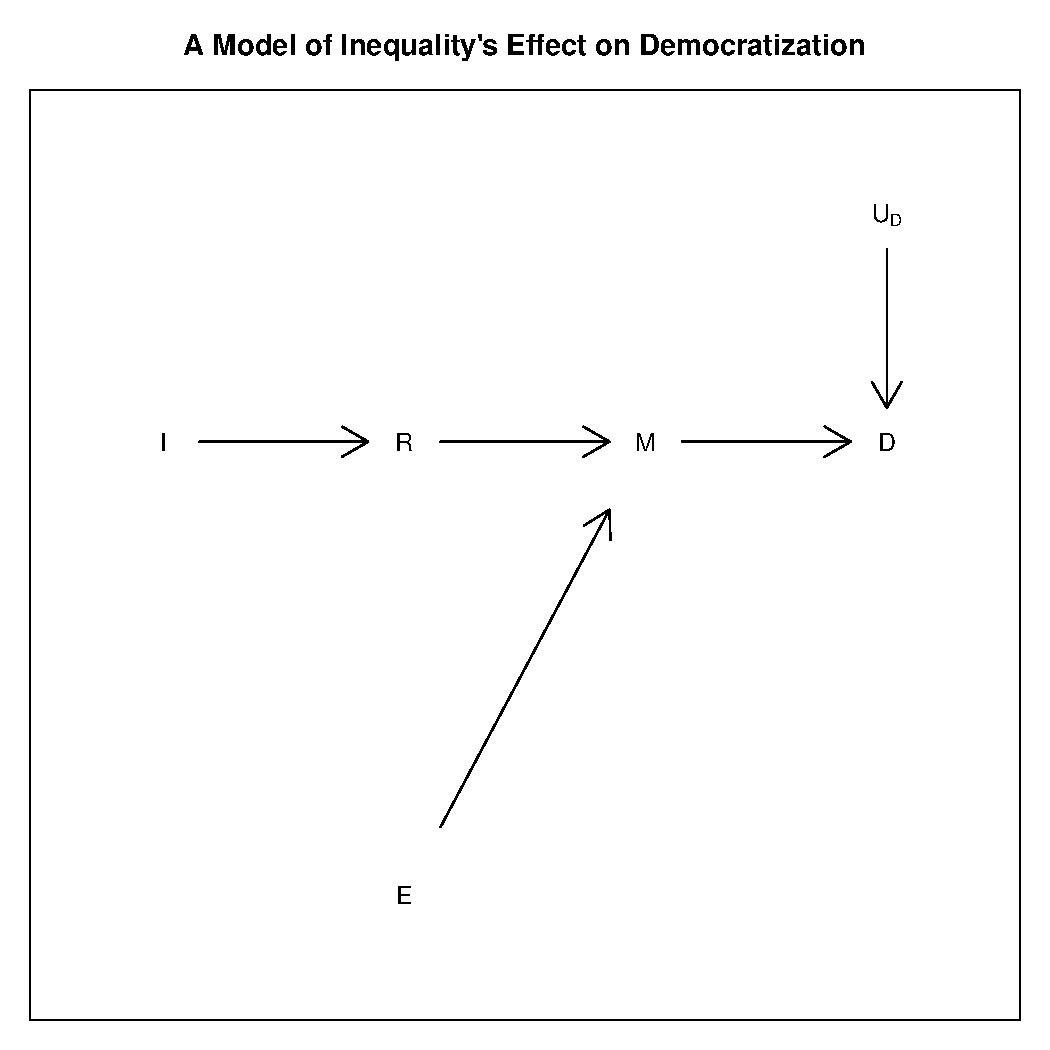
\includegraphics[width=0.8\linewidth]{ii_files/figure-latex/simpleDAG-1} 

}

\caption{A simple causal model in which high inequality ($I$) affects democratization ($D$) via redistributive demands and mass mobilization ($M$), which is also a function of ethnic homogeneity ($E$). The arrows show relations of causal dependence between variables.  The graph does not capture the ranges of the variables and the functional relations between them.}\label{fig:simpleDAG}
\end{figure}

Fundamentally, we treat causal models in this book as formal representations of \emph{beliefs} about how the world works---or, more specifically, about causal relations within a given domain. We might use a causal model to capture our own beliefs, a working simplification of our beliefs, or a set of potential beliefs that one might hold. The formalization of \emph{prior} beliefs in the form of a causal model is the starting point for research design and inference in this book's analytic framework. Using the democratization example, we will now walk through the three components of a causal model in which our beliefs get embedded: nodes, functions, and distributions.

\hypertarget{components-of-a-causal-model}{%
\subsection{Components of a Causal Model}\label{components-of-a-causal-model}}

The three components of a causal model are (i) the nodes---that is, the set of variables we are focused on and how are they defined (ii) the functional relations---which nodes are ``explained'' by which other nodes and how, and (iii) probability distributions over unexplained elements of a model.

\hypertarget{the-nodes}{%
\subsubsection{The nodes}\label{the-nodes}}

The first component of a causal model is the set of variables (nodes) across which the model characterizes causal relations. On the graph in Figure \ref{fig:simpleDAG}, the five included variables are represented by the five lettered nodes. (In addition we mark \(\theta^D\) on the graph though, as will be made clear, we will not think of this as a variable.)

In identifying the nodes, we also need to specify the \emph{ranges} over which they can vary. We might specify, for instance, that all nodes in the model are binary, taking on the values 0 or 1. We could, alternatively, define a set of categories across which a node ranges or allow a node to take on any real number value or any value between a set of bounds. \footnote{If we let \(\mathcal{R}\) denote a set of ranges for all nodes in the model, we can indicate \(X\)'s range, for instance, by writing \(\mathcal{R}(X)=\{0,1\}\). The nodes in a causal model together with their ranges---the triple \((\mathcal{U}, \mathcal{V}, \mathcal{R})\)---are sometimes called a \emph{signature}, \(\mathcal{S}\).}

Notice that some of these nodes have arrows pointing \emph{into} them: \(R, M\), and \(D\) are endogenous nodes, meaning that their values are determined entirely by other nodes in the model.

Other nodes have arrows pointing out of them but no arrows pointing into them: \(I\) and \(E\). \(I\) and \(E\) are ``exogenous'' nodes; they influence other nodes in the model but themselves have no causes specified in the model.

The \(\theta\) terms require a little more explanation since they do not describe substantive nodes. In our discussion above, we introduced \(\theta\) notation for representing types. Generally we can think of \(\theta\) terms on a causal graph as unobservable and unspecified features of a causal domain that affect outcomes. These might include random processes (noise) or contextual features that we are unable to identify or do not understand. We imagine them pointing into everynode, whether indicated or not. In all cases the work they do is to characterize what the value of a node will be, given the value of its parents.

We note that our notation for representing these unobservable, unspecified influences differs from that commonly found in the literature on causal models. In many treatments, these components are themselves referred to as ``exogenous'' variables, and often labelled as sets \(\mathcal U\), to be distinguished from the endogenous---named--variables often labelled as \(\mathcal V\). We will generally use \(\theta\) to denote these unobserved, unspecified influences to emphasize their particular role, as direct objects of interest in causal inquiry. As we will show, we can think of \(\theta\) nodes as capturing the functional relations between endogeneous variables and as being quantities of direct interest for causal inquiry. We more fully develop this point---returning to the notion of \(\theta\) terms as receptacles for causal effects---below.

\hypertarget{the-functions}{%
\subsubsection{The functions}\label{the-functions}}

Next, we need to specify our beliefs about the causal relations among the nodes in our model. How is the value of one node affected by, and how does it affect, the values of others? For each endogenous node---each node influenced by others in the model---we need to express beliefs about how its value is affected by its parents, its immediate causes.

The DAG already represents a critical part of these beliefs: the arrows, or directed edges, tell us \emph{which nodes we believe to be direct causal inputs into other nodes}. So, for instance, we believe that democratization (\(D\)) is determined jointly by mobilization (\(M\)) and some exogenous, unspecified factor (or set of factors), \(\theta^D\). As we have said, we can think of \(\theta^D\) as all of the other influences on democratization, besides mobilization, that we either do not know of or have decided not to explicitly include in the model. We believe, likewise, that \(M\) is determined by \(I\) and an unspecified exogenous factor (or set of factors), \(\theta^M\). And we are conceptualizing inequality (\(I\)) and ethnic heterogeneity (\(E\)) as shaped solely by factors exogenous to the model, captured by \(\theta^I\) and \(\theta^E\), respectively.

Beyond the beliefs captured by the arrows in a DAG, we can express more specific beliefs about causal relations in the form of a causal function.\footnote{The collection of all causal functions in the model can be denoted as \(\mathcal{F}\).} Specifying a function means writing down whatever general or theoretical knowledge we have about the direct causal relations between nodes. A function specifies how the value that one node takes on is determined by the values that other nodes---its parents---take on.

We can specify this relationship in a vast variety of ways. It is useful however to distinguish broadly between parametric and non-parametric approaches. We take a non-parametric approach in this book, but it is helpful to juxtapose that approach to a parametric one.

\textbf{Parametric approaches.} A parametric approach specifies a functional form that relates parents to children. For instance, we might model one node as a linear function of another and write \(D=\alpha + \beta M\), where \(\beta\) is a parameter that we do not know the value of at the outset of a study but about which we wish to learn. If we believe \(D\) to be linearly affected by \(M\) but also subject to forces that we do not yet understand and have not yet specified in our theory, then we might write: \(D=\alpha + \beta M+\theta^D\). In this function, \(\alpha, \beta\) might be the parameters of interest, with \(\theta^D\) treated merely as a random disturbance. We can be still more agnostic by, for example, including parameters that govern how other parameters operate. Consider, for instance the function, \(D=\beta M^{\theta^D}\). Here, \(D\) and \(M\) are linearly related if \(\theta^D=1\), but not otherwise.

Note that functions can be written to be quite specific or extremely general, depending on the state of prior knowledge about the phenomenon under investigation. The use of a structural model \emph{does not require precise knowledge of specific causal relations}, even of the functional forms through which two nodes are related.

\textbf{The non-parametric approach.} With discrete data, causal functions can take fully \emph{non-parametric} form, allowing for \emph{any possible relation} between parents and children. We use this framework for most of this book and thus spend some time developing the approach here.

We begin by returning to the concept of types. Drawing on our original four types from earlier in this chapter, we know that we can fully specify causal relations between a binary \(M\) and a binary \(D\) by allowing the node \(\theta_D\) to range across four possible values \(\{\theta^D_{10}, \theta^D_{01}, \theta^D_{00}, \theta^D_{11}\}\). For instance, \(\theta^D_{10}\) represents a negative causal effect of \(M\) on \(D\) while \(\theta^D_{00}\) represents \(D\) remaining at 0 regardless of \(M\). Put differently, \(\theta^D\) represents the non-parametric function that relates \(M\) to \(D\). We can formally specify \(D\)'s behavior as a function of \(M\) and \(\theta^D\) in the following way:

\[D(M, \theta^D_{ij}) = \left\{\begin{array}{ccc} i & \text{if} & M=0 \\ j & \text{if} & M=1 \end{array}\right.\]

Note that \(\theta^D\) ranges over \emph{all possible} functional forms between these two binary variables.

How should we think about what kind of \emph{thing} \(\theta^D\) is, in a more substantive sense? It is probably most helpful to think of \(\theta^D\) as an unknown and possibly random factor that conditions the effect of mobilization on democratization, determining whether \(M\) has a negative effect, a positive effect, no effect with democratization never occurring, or no effect with democratization bound to occur regardless of mobilization. Importantly, however, while we might think of \(\theta^D\) as an unknown or random quantity, in this formulation \(\theta^D\) should not be thought of as a nuisance---as ``noise'' that we would like to get rid of---but as \emph{the quantity that we want to learn about}: we want to know whether \(M\) likely had a positive, negative, or no effect on \(D\). We elaborate on this point at much greater length in Chapter \ref{questions}.

We can similarly use \(\theta\) terms to capture causal relations involving any number of parent nodes. Every substantively defined node, \(J\), in a graph can be thought of as having a \(\theta^J\) term pointing into it, and the (unobservable) value of \(\theta^J\) represents the mapping from \(J\)'s parents (if it has any) to the value of \(J\).

Applied to the binary nodes in Figure \ref{fig:simpleDAG}, \(\theta^J\) ranges as follows:

\begin{itemize}
\tightlist
\item
  \textbf{Nodes with no parents}: For an exogenous node, like \(I\) or \(E\), \(\theta^J\) represents an external ``assignment'' process that can take on one of two values, \(\theta^J_{0}\), meaning that \(J\) is ``assigned'' to \(0\) or \(\theta^J_{1}\), meaning that \(J\) is assigned to 1. For instance, \(\theta^I_{0}\) describes a case in which exogenous forces have generated low inequality.
\item
  \textbf{Binary nodes with 1 binary parent}: For endogenous node \(R\), with only one parent (\(I\)), \(\theta^R\) takes on one of four values of the form \(\theta^R_{ij}\) (our four original types, \(\theta^R_{10}\), \(\theta^R_{01}\), etc.).
\item
  \textbf{Binary nodes with 2 binary parents}: \(M\) has two parent nodes. Thus, \(\theta^M\) will take on a possible 16 values of the form \(\theta^M_{hijk}\) (\(\theta^M_{0000}\), \(\theta^M_{0001}\), etc.), using the syntax detailed earlier in this chapter.
\end{itemize}

\textbf{Nodal types and causal types.} For analytic applications later in the book, we will want to be able to think both about the type operating at a particular \emph{node} and about \emph{collections} of types operating across a model. We thus refer to \(\theta^J\) as a unit's \emph{nodal} causal type, or simply nodal type, for \(J\). We refer to the collection of nodal types across all nodes for a given unit (i.e., a case) as the case's \emph{unit causal type}, or simply \emph{causal type}, denoted by the vector \(\theta\).

If we hypothetically knew a unit's causal type---all nodal types for all nodes---then we would know everything there is to know about that unit. Since the nodal types of exogenous nodes include \emph{values} of all exogenous nodes, and the nodal types of all endogenous nodes specify how those nodes respond to all of their parents, a unit's causal type fully specifies all nodal values as well as all \emph{counterfactual} nodal values for a unit.

We will sometimes refer to the values of \(\theta\) as a unit's \emph{context}. This is because \(\theta\) captures all exogenous forces acting on a unit. This includes the assignment process driving the model's exogenous nodes (in our example, \(\theta^I\) and \(\theta^E\)) as well as all contextual factors that shape causal relations between nodes (\(\theta^R\), \(\theta^M\), and \(\theta^D\)). Put differently, \(\theta\) captures both how a unit reacts to situations and which situations it is reacting to. One implication is that there is no \emph{formal} distinction between a unit's type and a unit's situation---between, say, a hungry person, and a person who has had no food.

\begin{longtable}[]{@{}
  >{\centering\arraybackslash}p{(\columnwidth - 4\tabcolsep) * \real{0.22}}
  >{\centering\arraybackslash}p{(\columnwidth - 4\tabcolsep) * \real{0.16}}
  >{\centering\arraybackslash}p{(\columnwidth - 4\tabcolsep) * \real{0.62}}@{}}
\caption{\label{tab:NTCT}. Nodal types, causal types.}\tabularnewline
\toprule
\textbf{term} & \textbf{symbol} & \textbf{meaning} \\
\midrule
\endfirsthead
\toprule
\textbf{term} & \textbf{symbol} & \textbf{meaning} \\
\midrule
\endhead
nodal type & \(\theta^J\) & The way that node \(J\) responds to the values of its parents. Example: \(\theta^Y_{10}\): \(Y\) takes the value 1 if \(X=0\) and 0 if \(X=1\). \\
causal type & \(\theta\) & A causal type is a concatenation of nodal types, one for each node. Example: \((\theta^X_0, \theta^Y_{00})\), is a causal type that has \(X=0\) and that has \(Y=0\) no matter what the value of \(X\). \\
\bottomrule
\end{longtable}

A few important aspects of causal functions are worth highlighting.

\begin{enumerate}
\def\labelenumi{\arabic{enumi}.}
\item
  These functions express \emph{causal} beliefs. When we write \(D=\beta M\) as a function, we do not just mean that we believe the values of \(M\) and \(D\) in the world to be linearly related. We mean that we believe that the value of \(M\) \emph{determines} the value of \(D\) through this linear function. Functions are, in this sense, \emph{directional} statements, with causes on the righthand side and an outcome on the left.
\item
  The collection of simple functions that map from the values of parents of a given node to the values of that node are sufficient to represent potentially complex webs of causal relations. For each node, we do not need to think through entire sequences of causation that might precede it. We need only specify how we believe it to be affected by its parents---that is to say, those nodes pointing directly into it. Our outcome of interest, \(D\), may be shaped by multiple, long chains of causality. To theorize how \(D\) is generated, however, we write down how we believe \(D\) is shaped by its parent---its direct cause, \(M\). We then, separately, express a belief about how \(M\) is shaped by \emph{its} parents, \(R\) and \(E\). A node's function must include as inputs all, and only, those nodes that point directly into that node.\footnote{The set of a node's parents is required to be minimal in the sense that a node is not included among the parents if, given the other parents, the child does not depend on it in any state that arises with positive probability.}
\item
  As in the general potential-outcomes framework, all relations in a causal model are conceptualized as deterministic at the case level. Yet, there is not as much at stake here as one might think at first; by this we simply mean that a node's value is \emph{determined} by the values of its parents \emph{along with} any stochastic or unknown components. We express uncertainty about causal relations, however, as unknown parameters, such as the causal types \(\theta\).
\end{enumerate}

\hypertarget{the-distributions}{%
\subsubsection{The distributions}\label{the-distributions}}

Putting causal structure and causal functions together gives us a \emph{structural causal model.} In a structural causal model, all endogenous nodes are, either directly or by implication, functions of a case's context (the values of the set of exogenous nodes).\footnote{More formally, a \textbf{structural causal model} \emph{over} signature \(\mathcal{S}=<\mathcal{U},\mathcal{V},\mathcal{R}>\) is a pair \(<\mathcal{S}, \mathcal{F}>\), where \(\mathcal{F}\) is a set of ordered structural equations containing a function \(f_i\) for each element \(Y\in \mathcal{V}\). We say that \(\mathcal{F}\) is a set of ordered structural equations if no node is its own descendant and if no element in \(\mathcal{U}\) is parent to more than one element of \(\mathcal{V}\). This last condition can be achieved by shifting any parent of multiple children in \(\mathcal{U}\) to \(\mathcal{V}\). This definition thus includes an assumption of acyclicity, which is not found in all definitions in the literature.} What we have not yet inscribed into the model, however, is beliefs about how \emph{likely} or \emph{common} different kinds of contexts might be.

Thus, for instance, a structural causal model consistent with Figure \ref{fig:simpleDAG} stipulates which nodes may have effects on which other nodes. But it says nothing in itself about the distribution of values of either the exogenous nodes or of the causal relations between nodes.\footnote{Thus \(P(d|i,e, u_D)\) would defined by this structural model (as a degenerate distribution), but \(P(i)\), \(P(e)\), \(P(u_D)\), and \(P(i,e, u_D)\) would not be.} We have not said anything, for instance, about how common high inequality is across the relevant domain of cases or how common ethnic homogeneity is. Put differently, we have said nothing about the \emph{distribution} of \(\theta^I\) or of \(\theta^E\). Similarly, we have said nothing yet about how commonly mobilization has positive, negative, or null effects of democratization---that is, the distribution of \(\theta^D\)---or about how commonly \(I\) and \(E\) have different possible joint causal effects on \(M\) (the distribution of \(\theta^M\)).

In many research situations, we will have or want to posit a set of prior beliefs about how the world works under different conditions and about what kinds of conditions are more likely than others. We can express these beliefs about context as probability distributions over the model's \(\theta^J\) terms. For instance, our structural causal model might tell us that \(E\) and \(R\) can jointly affect \(M\). We might, then, add to this a belief about \(\theta^M\) such that, in the population of interest, redistribution rarely has a positive effect on mobilization when ethnic homogeneity is low. We would thus be putting a low probability on the nodal types for \(M\) in which \(R\) has a positive effect on \(M\) when \(E=0\), relative to \(M\)'s other nodal types.\footnote{Ordering the parent nodes alphabetically, the types we would be setting to a low probability would be \(\theta^M_{0010}, \theta^M_{0110}, \theta^M_{0111}, \theta^M_{0011}\).}

We might add to this the belief that \(E=1\) in only 10\% of cases in the population of interest, thus setting a 0.1 probability on \(\theta^E_1\). Note that these two beliefs jointly imply that \(R\) will rarely have a positive effect on \(M\).

As with functions, we can also (and typically would) build uncertainty into our beliefs about the shares of different nodal types in the population. We do this by specifying a \emph{distribution} over possible ``share'' allocations.\footnote{More strictly our uncertainty is over probabilities. However it is sometimes more intuitive to describe uncertainty over shares. The distinction is not important for the applications later in which we typically assume units are independently drawn from a large population.} For instance, we can specify a distribution over the shares of cases with ethnic homogeneity (\(\theta^E_1\)), and a distribution over the shares of \(\theta^M\) types, with our degrees of uncertainty captured by each distribution's variance. (More on these distributions in Chapter \ref{bayeschapter}.)

In the default setup, we assume that each \(\theta\) term (\(\theta^I, \theta^E, \theta^R\), etc.) is generated independently of the others.

While this is not without loss of generality, it is not as constraining as it might at first appear: any graph in which two \(\theta\) terms are \emph{not} independent can be replaced by a graph in which these two terms are themselves generated by a common, third \(\theta\) term.\footnote{Operationally, in the \texttt{CausalQueries} package, we can specify nodal types as having joint distributions.} This independence feature is critical for being able to read off relations of conditional independence from a graph (see Box below). If it cannot be defended then the graph needs to be modified to communicate that \(\theta\)s are not independent, typically using two headed arrows. More on this in section \ref{graphing}.\\

\begin{headerbox}

\leavevmode\hypertarget{markov}{}%
\begin{center}
\textbf{Technical Note on the Markov Property}

\end{center}

The assumptions that no node is its own descendant and that the \(\theta\) terms are generated independently make the model \emph{Markovian}, and the parents of a given node are Markovian parents. Knowing the set of Markovian parents allows one to write relatively simple factorizations of a joint probability distribution, exploiting the fact (``the Markov condition'') that all nodes are \emph{conditionally independent} of their nondescendants, conditional on their parents: nodes \(A\) and \(B\) are ``conditionally independent'' given \(C\) if \(P(a|b,c) = P(a|c)\) for all values of \(a, b\) and \(c\).\\
To see how this Markovian property allows for simple factorization of \(P\) for Figure \ref{fig:simpleDAG}, note that \(P(X, R, Y)\) can always be written as:
\[P(X, R, Y) = P(X)P(R|X)P(Y|R, X)\]
If we believe, as in the figure, that \(X\) causes \(Y\) only through \(R\) then we have the slightly simpler factorization:
\[P(X, R, Y) = P(X)P(R|X)P(Y|R)\]
Or, more generally:

\begin{equation} 
P(v_1,v_2,\dots v_n) = \prod P(v_i|pa_i)
\label{eq:markov}
\end{equation}

The distribution \(P\) on \(\theta\) induces a joint probability distribution on \(\mathcal{V}\) that captures not just information about how likely different states are to arise but also the relations of conditional independence between nodes that are implied by the underlying causal process. For example, if we thought that \(X\) caused \(Y\) via \(R\) (and only via \(R\)), we would then hold that \(P(Y | R) = P(Y | X, R)\): in other words if \(X\) matters for \(Y\) only via \(R\) then, conditional on \(R\), \(X\) should not be informative about \(Y\).\\
In this way, a probability distribution \(P\) over a set of nodes can be consistent with some causal models but not others. This does not, however, mean that a specific causal model can be extracted from \(P\). To demonstrate with a simple example for two nodes, any probability distribution on \((X,Y)\) with \(P(x)\neq P(x|y)\) is consistent both with a model in which \(X\) is a parent of \(Y\) and with a model in which \(Y\) is a parent of \(X\).

\end{headerbox}

Once we introduce beliefs about the distribution of values of the exogenous terms (in our setup, the \(\theta\) terms) in a model, we have specified a \emph{probabilistic causal model.} We need not say much more, for the moment, about the probabilistic components of causal models. But to foreshadow the argument to come, our prior beliefs about the likelihoods of different contexts play a central role in the framework that we develop here. We will see how the encoding of contextual knowledge---beliefs that some kinds of conditions and causal effects are more common than others---forms a key foundation for causal inference. At the same time, our expressions of \emph{uncertainty} about context represent scope for learning: it is the very things that we are, at a study's outset, uncertain about that we can update our beliefs about as we encounter evidence.

\hypertarget{graphing-models-and-using-graphs}{%
\section{Graphing models and using graphs}\label{graphing-models-and-using-graphs}}

While we have been speaking to causal graphs throughout this chapter, we want to take some time to unpack their core features and uses. A key benefit of causal models is that they lend themselves to graphical representations; in turn, graphs constructed according to particular rules can aid causal analysis. In the next subsection we discuss a set of rules for representing a model in graphical form. The following subsection then demonstrates how access to a graph facilitates causal inference.

\hypertarget{graphing}{%
\subsection{Rules for graphing causal models}\label{graphing}}

The diagram in Figure \ref{fig:simpleDAG} is a causal DAG \citep{hernan2006instruments}. We endow it with the interpretation that an arrow from a parent to a child means that a change in the parent can, under some circumstances, induce a change in the child. Though we have already been making use of this causal graph to help us visualize elements of a causal model, we now explicitly point out a number of general features of causal graphs as we will be using them throughout this book. Causal graphs have their own distinctive ``grammar,'' a set of rules that give them important analytic features.

\textbf{Directed, acyclic.} A causal graph represents elements of a causal model as a set of nodes (or vertices), representing nodes, connected by a collection of single-headed arrows (or directed edges). We draw an arrow from node \(A\) to node \(B\) if and only if we believe that \(A\) can have a direct effect on \(B\). The resulting diagram is a \emph{directed acyclic} graph (DAG) if there are no paths along directed edges that lead from any node back to itself---i.e., if the graph contains no causal cycles. The absence of cycles (or ``feedback loops'') is less constraining than it might appear at first. In particular if one thinks that \(A\) today causes \(B\) tomorrow which in turn causes \(A\) today, we can represent this as \(A_1 \rightarrow B \rightarrow A_2\) rather than \(A \leftrightarrow B\). That is, we timestamp the nodes, turning what might informally appear as feedback into a non-cyclical chain.

\textbf{Meaning of missing arrows.} The \emph{absence} of an arrow between \(A\) and \(B\) means that \(A\) is not a direct cause of \(B\).\footnote{By ``direct'' we mean that the \(A\) is a parent of \(B\): i.e., the effect of \(A\) on \(B\) is not fully mediated by one or more other nodes in the model.} Here lies an important asymmetry: drawing an \(A \rightarrow B\) arrow does not mean that we know that \(A\) \emph{does} directly cause \(B\); but omitting such an arrow implies that we know that \(A\) does \emph{not} directly cause \(B\). We say more, in other words, with the arrows we omit than with the arrows that we include.

Returning to Figure \ref{fig:simpleDAG}, we have here expressed the belief that redistributive preferences exert no direct effect on democratization; we have done so by \emph{not} drawing an arrow directly from \(R\) to \(D\). In the context of this model, saying that redistributive preferences have no direct effect on democratization is to say that any effect of redistributive preferences on democratization \emph{must} run through mobilization; there is no other pathway through which such an effect can operate. This might be a way of encoding the knowledge that mass preferences for redistribution cannot induce autocratic elites to liberalize the regime absent collective action in pursuit of those preferences.

The same goes for the effects of \(I\) on \(M\), \(I\) on \(D\), and \(E\) on \(D\): the graph in Figure \ref{fig:simpleDAG} implies that we believe that these effects also do not operate directly, but only along the indicated, mediated paths.

\textbf{Sometimes-causes.} The existence of an arrow from \(A\) to \(B\) does not imply that \(A\) always has a direct effect on \(B\). Consider, for instance, the arrow running from \(R\) to \(M\). The existence of this arrow requires that \(R\) appears somewhere in \(M\)'s functional equation, as a node's functional equation must include all nodes pointing directly into it. Imagine, though, that \(M\)'s causal function were specified as: \(M = RE\). This function would allow for the \emph{possibility} that \(R\) affects \(M\), as it will whenever \(E=1\). However, it would also allow that \(R\) will have no effect, as it will when \(E=0\).

\textbf{No excluded common causes.} Any cause common to multiple nodes on a graph must itself be represented on the graph. If \(A\) and \(B\) on a graph are both affected by some third node, \(C\), then we must represent this common cause. Thus, for instance, the graph in Figure \ref{fig:simpleDAG} implies that \(I\) and \(E\) have no common cause. If in fact we believed that a country's level of inequality and its ethnic composition were both shaped by, say, its colonial heritage, then this DAG would \emph{not} be an accurate representation of our beliefs about the world. To make it accurate, we would need to add to the graph a node capturing that colonial heritage and include arrows running from colonial heritage to both \(I\) and \(E\).

This rule ensures that the graph captures all potential correlations among nodes that are implied by our beliefs. If \(I\) and \(E\) are in fact driven by some common cause, then this means not just that these two nodes will be correlated but also that each will be correlated with any consequences of the other. For instance, a common cause of \(I\) and \(E\) would also imply a correlation between \(R\) and \(E\). \(R\) and \(E\) are implied to be independent in the current graph but would be implied to be correlated if a common node pointed into both \(I\) and \(E\).

Of particular interest in Figure \ref{fig:simpleDAG} is the implied independence of \(\theta^J\)'s from one another. Imagine, for instance, that the distribution of \(\theta^D\) were different if \(I=0\) or \(I=1\). This would represent a classic form of confounding: the assignment of cases to values on the explanatory node would be correlated with the case's potential outcomes on \(D\). The omission of any such pathway is precisely equivalent to expressing the belief that \(I\) is exogenous, i.e., (as if) randomly assigned.

\textbf{Representing unobserved confounding.} It may be however that there are common causes for nodes that we simply do not understand. We might believe that some unknown factor (partially) determines both \(I\) and \(D\), which is the same as saying that \(\theta^I\) and \(\theta^D\) are not independently distributed. If we were to represent the \(\theta\) terms on the graph we might then want to represent a single term \((\theta^I, \theta^D)\) that points into both \(I\) and \(D\). Usually however the \(\theta\) terms are omitted from graphs and in this case we would represent the unobserved confounding by adding a dotted line, or a two headed arrow, connecting nodes whose unknown components are not independent. Figure \ref{fig:simpleDAGb} illustrates. We address this kind of unobserved confounding later in the book and show how we can seek to learn about the joint distribution of nodal types in such situations.

\begin{figure}

{\centering 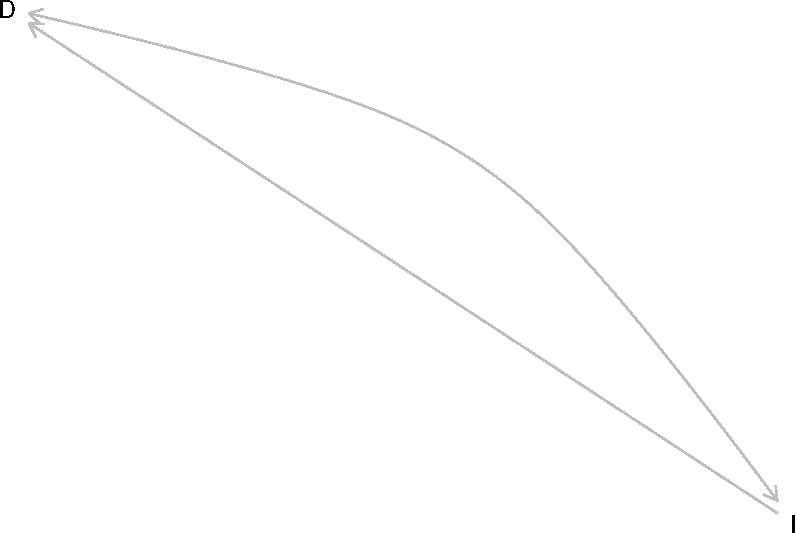
\includegraphics[width=0.6\linewidth]{ii_files/figure-latex/simpleDAGb-1} 

}

\caption{A DAG with unobserved confounding}\label{fig:simpleDAGb}
\end{figure}

\textbf{Licence to exclude nodes.} The flip side of the ``no excluded common causes'' rule is that a causal graph, to do the work it must do, does not need to include everything we know about a substantive domain of interest. We may know quite a lot about the causes of economic inequality, for example. But we can safely omit any other factor from the graph as long \emph{as it does not affect multiple nodes in the model.} Indeed, \(\theta^I\) in Figure \ref{fig:simpleDAG} already implicitly captures all factors that affect \(I\), just as \(\theta^D\) captures all factors \emph{other than} mobilization that affect democratization. We may be aware of a vast range of forces shaping whether countries democratize, but choose to bracket them for the purposes of an examination of the role of economic inequality. This bracketing is permissible as long as none of these unspecified factors also act on other nodes included in the model.

\textbf{We can't read functional equations from a graph.} As should be clear, a DAG does not represent all features of a causal model. What it does record is which nodes enter into the structural equation for every other node: what can directly cause what. But the DAG contains no other information about the form of those causal relations. Thus, for instance, the DAG in Figure \ref{fig:simpleDAG} tells us that \(M\) is function of both \(R\) and \(E\), but it does not tell us whether that joint effect is additive (\(R\) and \(E\) separately increase mobilization) or interactive (the effect of each depends on the value of the other), or whether either effect is linear, concave, or something else. This lack of information about functional forms often puzzles those encountering causal graphs for the first time: surely it would be convenient to visually differentiate, say, additive from interactive effects. As one thinks about the variety of possible causal functions, however, it quickly becomes clear that there would be no simple visual way of capturing all possible functional relations. Moreover, causal graphs do not require functional statements to perform their main analytic purpose---a purpose to which we now turn.

\hypertarget{conditional-independence-from-dags}{%
\subsection{Conditional independence from DAGs}\label{conditional-independence-from-dags}}

If we encode our prior knowledge using the grammar of a causal graph, we can put that knowledge to work for us in powerful ways. In particular, the rules of DAG-construction allow for an easy reading of the \emph{conditional independencies} implied by our beliefs. (For another, somewhat more extended treatment of the ideas in this section, see \citet{rohrer2018thinking}.)

To begin thinking about conditional independence, it can be helpful to conceptualize dependencies between nodes as generating \emph{flows of information}. Let us first consider a simple relationship of dependence. Returning to Figure \ref{fig:simpleDAG}, the arrow running from \(I\) to \(R\), implying a direct causal dependency, means that we expect \(I\) and \(R\) to be correlated. Put differently, observing the value of one of these nodes also gives us information about the value of the other. If we measured redistributive preferences, the graph implies that we would also be in a better position to infer the level of inequality, and vice versa. Likewise, \(I\) and \(M\) are also linked in a relationship of dependence: since inequality can affect mobilization (through \(R\)), knowing the the level of inequality would allow us to improve our estimate of the level of mobilization and vice versa.

In contrast, consider \(I\) and \(E\), which are in this graph indicated as being \emph{independent} of one another. Learning the level of inequality, according to this graph, would give us no information whatsoever about the degree of ethnic homogeneity, and vice-versa.

Moreover, sometimes what we learn depends on \emph{what we already know.} Suppose that we already knew the level of redistributive preferences. Would we then be in a position to learn about the level of inequality by observing the level of mobilization? According to this graph we would not: since the causal link---and, hence, flow of information between \(I\) and \(M\)---runs through \(R\), and we already know \(R\), there is nothing left to be learned about \(I\) by also observing \(M\). Anything we could have learned about inequality by observing mobilization is already captured by the level of redistributive preferences, which we have already seen. In other words, if we were not to include \(R\) in the causal model, then \(I\) and \(M\) would be dependent and informative about each other. When we do include \(R\) in the causal graph, \(I\) and \(M\) are independent of one another and, hence, uninformative about each other. We can express this idea by saying that \(I\) and \(M\) are \emph{conditionally independent given \(R\)}.

We say that two nodes, \(A\) and \(C\), are ``conditionally independent'' given a set of nodes \(\mathcal B\) if, once we have knowledge of the values in \(\mathcal B\), knowledge of \(A\) provides no information about \(C\) and vice-versa. Taking \(\mathcal B\) into account thus ``breaks'' any relationship that might exist unconditionally between \(A\) and \(C\).

To take up another example, suppose that war is a cause of both military casualties and price inflation, as depicted in Figure \ref{fig:warDAG}. Casualties and inflation will then be (unconditionally) correlated with one another because of their shared cause. If we learn that there have been military casualties, this information will lead us to think it more likely that there is also war and, in turn, price inflation (and vice versa). However, assuming that war is their only common cause, we would say that military casualties and price inflation are \emph{conditionally independent given war.} If we already know that there is war, then we can learn nothing further about the level of casualties (price inflation) by learning about price inflation (casualties). We can think of war, when observed, as blocking the flow of information between its two consequences; everything we would learn about inflation from casualties is already contained in the observation that there is war. Put differently, if we were just to look at cases where war is present (i.e., if we hold war constant), we should find no correlation between military casualties and price inflation; likewise, for cases in which war is absent.

\begin{figure}

{\centering 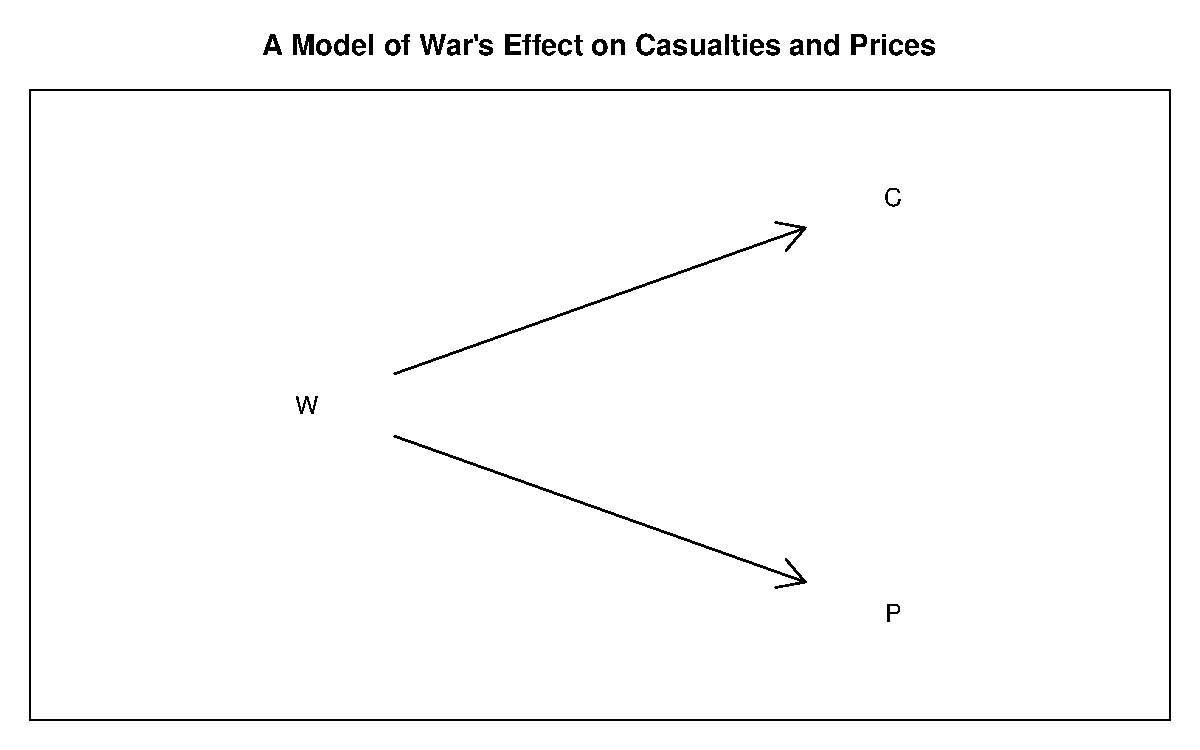
\includegraphics[width=0.6\linewidth]{ii_files/figure-latex/warDAG-1} 

}

\caption{This graph represents a simple causal model in which war ($W$) affects both military casualties ($C$) and price inflation ($P$).}\label{fig:warDAG}
\end{figure}

Relations of conditional independence are central to the strategy of statistical control, or covariate adjustment, in correlation-based forms of causal inference, such as regression. In a regression framework, identifying the causal effect of an explanatory node, \(X\), on a dependent node, \(Y\), requires the assumption that \(X\)'s value is conditionally independent of \(Y\)'s potential outcomes (over values of \(X\)) given the model's covariates. To draw a causal inference from a regression coefficient, in other words, we have to believe that including the covariates in the model ``breaks'' any biasing correlation between the value of the causal node and its unit-level effect.

As we will explore, however, relations of conditional independence are also of more general interest in that they tell us, given a model, \emph{when information about one feature of the world may be informative about another feature of the world, given what we already know}. By identifying the possibilities for learning, relations of conditional independence can thus guide research design. We discuss these research-design implications in Chapter \ref{pt}, but focus here on showing how relations of conditional independence operate on a DAG.

To see more systematically how a DAG can reveal conditional independencies, it is useful spell out three elemental structures according to which which information can flow across a causal graph:

\begin{figure}

{\centering 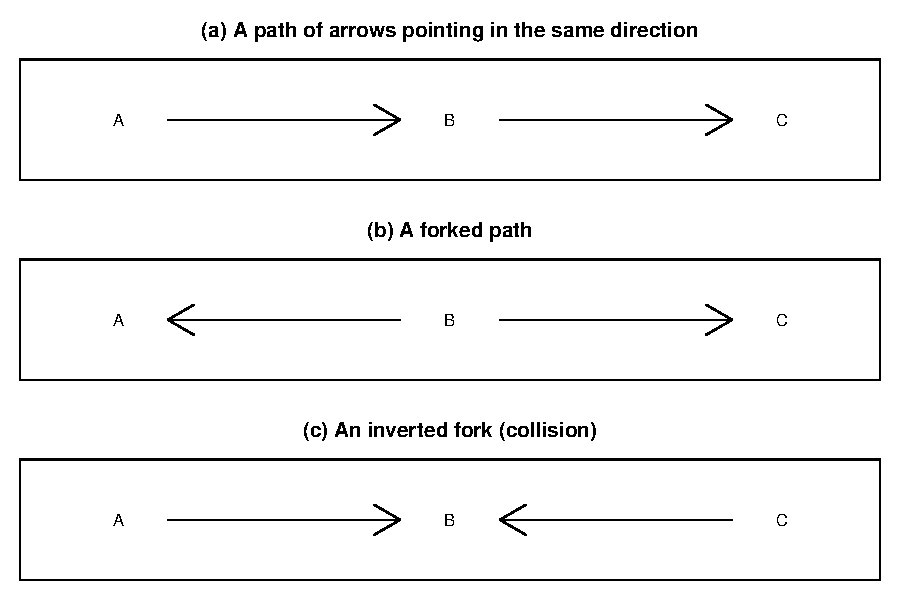
\includegraphics[width=0.7\linewidth]{ii_files/figure-latex/pathsexp-1} 

}

\caption{Three elemental relations of conditional independence.}\label{fig:pathsexp}
\end{figure}

(1a) Information can flow unconditionally along a path of arrows pointing in the same direction. In Panel 1 of Figure \ref{fig:pathsexp}, information flows across all three nodes. Learning about any one will tell us something about the other two.

(1b) Learning the value of a node along a path of arrows pointing in the same direction \emph{blocks} flows of information across that node. Knowing the value of \(B\) in Panel 1 renders \(A\) no longer informative about \(C\), and vice versa: anything that \(A\) might tell us about \(C\) is already captured by the information about \(B\).

(2a) Information can flow unconditionally across the branches of any forked path. In Panel 2 learning only \(A\) can provide information about \(C\) and vice-versa.

(2b) Learning the value of the node at the forking point blocks \emph{flows} of information across the branches of a forked path. In Panel 2, learning \(A\) provides no information about \(C\) if we already know the value of \(B\).\footnote{Readers may recognize this statement as the logic of adjusting for a confound that is a cause of both an explanatory node and a dependent node in order to achieve conditional independence.}

(3a) When two or more arrowheads collide, generating an inverted fork, there is no unconditional flow of information between the incoming sequences of arrows. In Panel 3, learning only \(A\) provides no information about \(C\), and vice-versa.

(3b) Collisions can be sites of \emph{conditional} flows of information. In the jargon of causal graphs, \(B\) in Panel 3 is a ``collider'' for \(A\) and \(C\).\footnote{In the familial language of causal models, a collider is a child of two or more parents.} Although information does not flow unconditionally across colliding sequences, it does flow across them \emph{conditional} on knowing the value of the collider node or any of its downstream consequences. In Panel 3, learning \(A\) \emph{does} provide new information about \(C\), and vice-versa, \emph{if} we also know the value of \(B\) (or, in principle, the value of anything that \(B\) causes).

The last point is somewhat counter-intuitive and warrants further discussion. It is easy enough to see that, for two nodes that are correlated unconditionally, that correlation can be ``broken'' by controlling for a third node. In the case of collision, two nodes that are \emph{not} correlated when taken by themselves \emph{become} correlated when we condition on (i.e., learn the value of) a third node, the collider. The reason is in fact quite straightforward once one sees it: if an outcome is a joint function of two inputs, then if we know the outcome, information about one of the inputs can provide information about the other input. For example, if I know that you have brown eyes, then learning that your mother has blue eyes makes me more confident that your father has brown eyes.

Looking back at our democratization DAG in Figure \ref{fig:simpleDAG}, \(M\) is a collider for \(R\) and \(E\), its two inputs. Suppose that we again have the functional equation \(M=RE\). Knowing about redistributive preferences alone provides no information whatsoever about ethnic homogeneity since the two are determined independently of one another. On the other hand, imagine that we already know that there was no mobilization. Now, if we observe that there \emph{were} redistributive preferences, we can figure out the level of ethnic homogeneity: it must be 0. (And likewise in going from homogeneity to preferences.)

Using these basic principles, conditional independencies can be read off of any DAG. We do so by checking every path connecting two nodes of interest and ask whether, along those paths, the flow of information is open or blocked, given any other nodes whose values are already observed. Conditional independence is established when \emph{all} paths are blocked given what we already know; otherwise, conditional independence is absent.

Following \citet{pearl2000causality}, we will sometimes refer to relations of conditional independence using the concept of \emph{d-separation.} We say that variable set \(\mathcal C\) \(d-\)separates variable set \(\mathcal A\) from variable set \(\mathcal B\) if \(\mathcal A\) and \(\mathcal B\) are conditionally independent given \(\mathcal C\). We say that \(\mathcal A\) and \(\mathcal B\) are \(d-\)connected given \(\mathcal C\) if \(\mathcal A\) and \(\mathcal B\) are \emph{not} conditionally independent given \(\mathcal C\).

\hypertarget{simplifying-models}{%
\subsection{Simplifying models}\label{simplifying-models}}

It is very easy to write down a model that is too complex to use effectively. In such cases we often seek simpler models that are consistent with models we have in mind but contain fewer nodes or more limited variation. In general this is possible but caution has to be taken to ensure that simplified models are indeed consistent with the original model.

Fortunately the mapping between graphs and relations of conditional independence give guidance for determining when and how it is possible to simplify models. We focus discussion on simplifications that involve node elimination and conditioning on nodes.

\hypertarget{eliminating-nodes}{%
\subsubsection{Eliminating nodes}\label{eliminating-nodes}}

If we want to eliminate a node the key rule is that the new model (and graph) must take into account:

\begin{enumerate}
\def\labelenumi{(\alph{enumi})}
\tightlist
\item
  all \emph{dependencies} among remaining nodes and
\item
  all \emph{variation} generated by the eliminated node.
\end{enumerate}

We can work out what this means, separately, for eliminating \emph{endogenous} nodes and for eliminating \emph{exogenous} nodes.

\emph{Eliminating endogenous nodes}

Eliminating an endogenous node means removing a node with parents (direct causes) represented on the graph. If the node also has one or more children, then the node captures a dependency: it links its parents to its children. When we eliminate this node, preserving these dependencies requires that all of the eliminated node's parents adopt---become parents of---all of the eliminated node's children. Thus, for instance if we had a model in which \(A \rightarrow M \leftarrow B\) and \(M \rightarrow Y\), if we were to eliminate \(M\), \(M\)'s parents (\(A\) and \(B\)) would need to adopt \(M\)'s child, \(Y\).

More intuitively, when we simplify away a mediator, we need to make sure that we preserve the causal relationships being mediated---both those among substantive variables and any random shocks at the mediating causal steps.\footnote{Eliminating endogenous nodes may also operate via ``encapsulated conditional probability distributions'' \citep{koller2009probabilistic} wherein a system of nodes, \(\{Z_i\}\) is represented by a single node, \(Z\), that takes the parents of \(\{Z_i\}\) not in \(\{Z_i\}\) as parents to \(Z\) and issues the children of \((Z_i)\) that are not in \((Z_i)\) as children. However, this is not a fundamental alteration of the graph.}

\emph{Eliminating exogenous nodes}

What about eliminating exogenous nodes---nodes with no parents? For the most part, exogenous nodes cannot be eliminated, but must either be replaced by or incorporated into \(U\) (or \(\theta\)) terms. The reason is that we need preserve any dependencies or variation generated by the exogenous node. Figure \ref{fig:elimrules} walks through four different situations in which we might want to simplify away the exogenous node, \(X\). (Here we use the more generic \(U\) notation, though the same principles apply if these are type-receptacles \(\theta\).)

\begin{figure}

{\centering 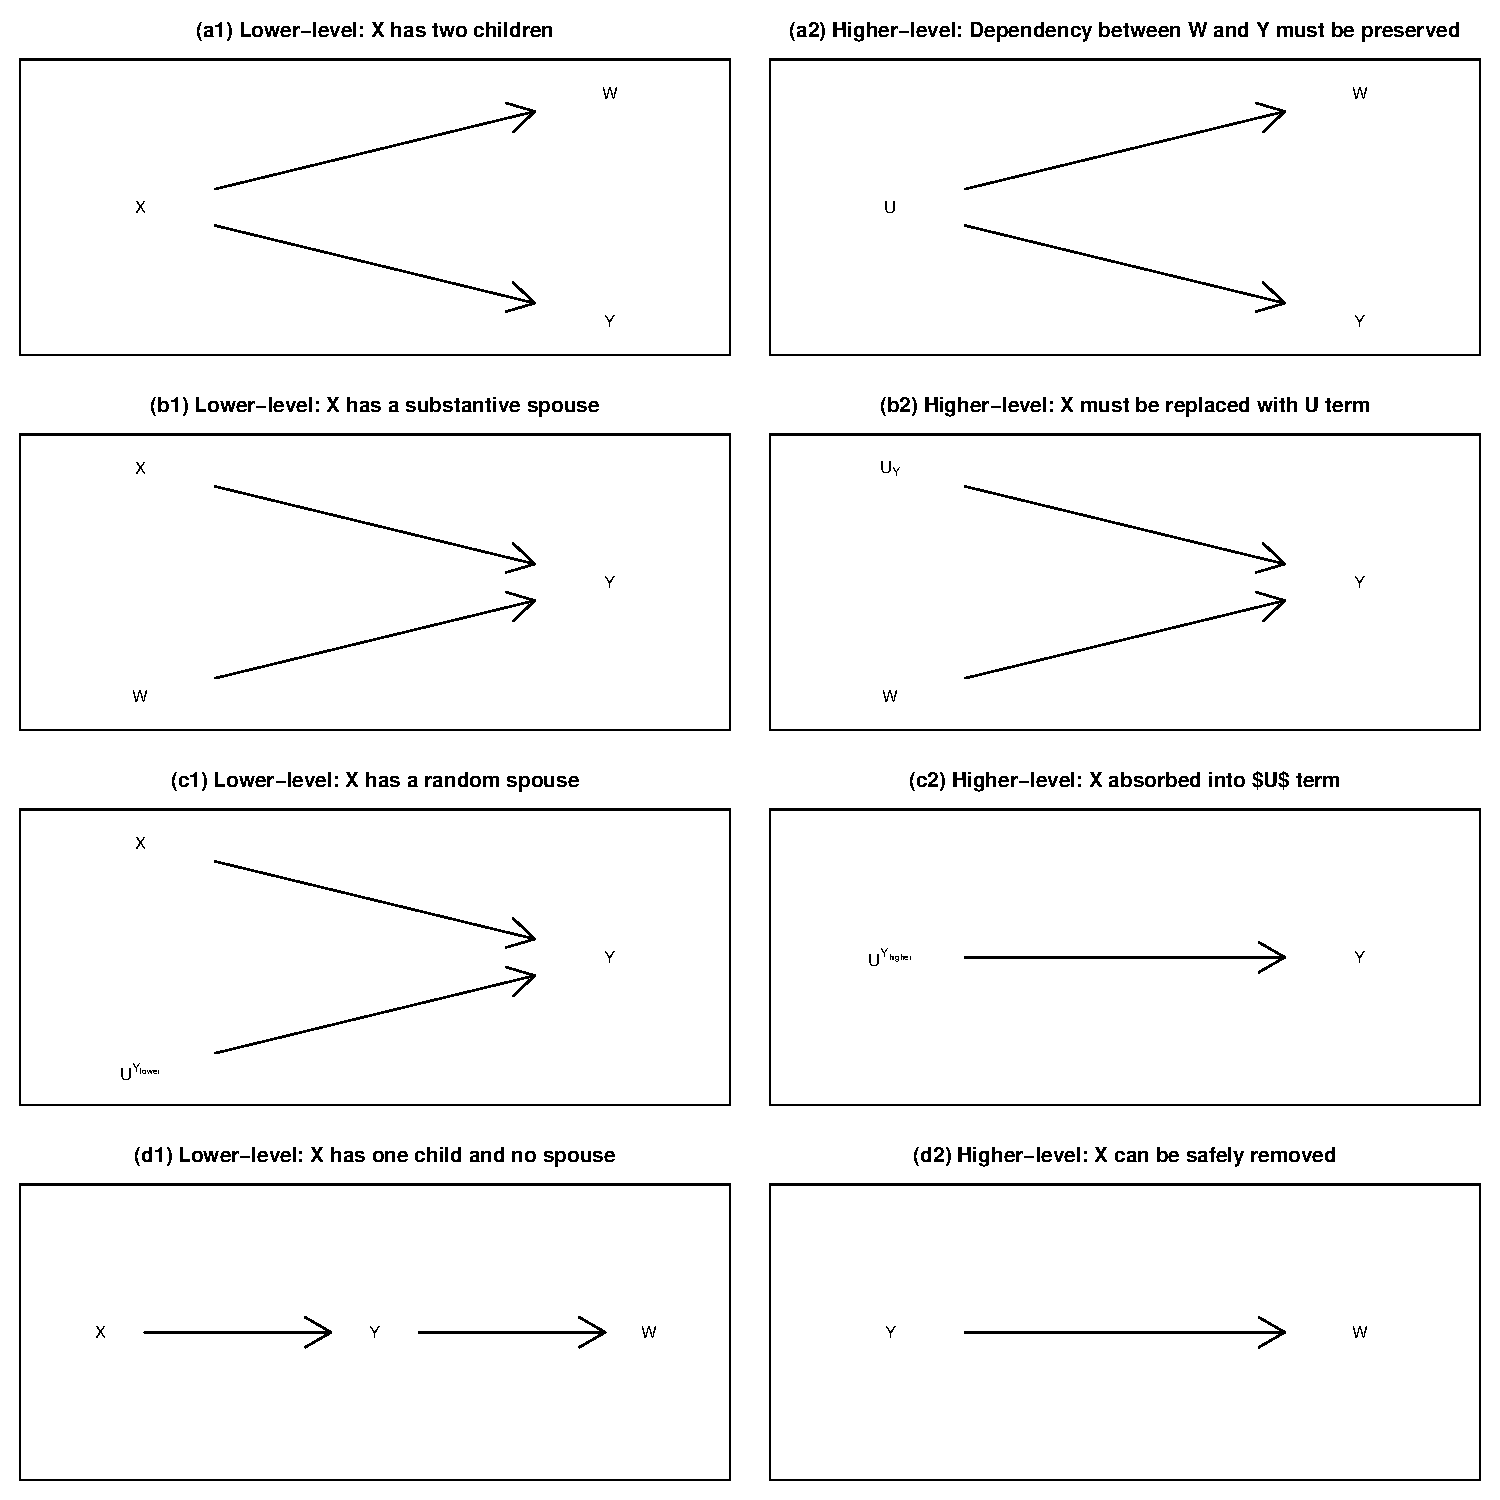
\includegraphics[width=.9\textwidth]{ii_files/figure-latex/elimrules-1} 

}

\caption{Basic principles for eliminating exogenous nodes.}\label{fig:elimrules}
\end{figure}

\begin{itemize}
\tightlist
\item
  \emph{Multiple children.} In (a1), we start with a model in which \(X\) has two children, thus generating a dependency between \(W\) and \(Y\). If we eliminate \(X\), we must preserve this dependency. We can do so, as pictured in (a2), by replacing \(X\) with a \(\theta\) term that points into both \(W\) and \(Y\). By convention, we could, alternatively, convey the same information with a dashed, undirected line between \(W\) and \(Y\). Though we are no longer specifying what it is that connects \(W\) and \(Y\), the correlation itself is retained.
\item
  \emph{Substantive spouse.} In (b1), \(X\) has a spouse that is substantively specified, \(W\). If we eliminate \(X\), we have to preserve the fact that \(Y\) is not fully determined by \(W\); \emph{something} else also generates variation in \(Y\). We thus need to replace \(X\) with a \(\theta\) term, \(\theta^Y\), to capture the variation in \(Y\) that is not accounted for by \(W\).
\item
  \emph{\(\theta\)-term spouse.} In (c1), \(X\) has a spouse that is \emph{not} substantively specified, \(U^{Y}\). Eliminating \(X\) requires, again, capturing the variance that it generates as a random input. As we already have a \(\theta\) term pointing only into \(Y\), we can substitute in \(\theta^{Y}_\text{mod}\), which represents both \(U^{Y}\) and the variance generated by \(X\).\footnote{This aggregation cannot occur if \(\theta^{Y}\) also has another child, \(W\), that is not a child of \(X\) since then we would be representing \(Y\)'s and \(W\)'s random components as identical, which they are not in the original graph.}
\item
  \emph{One child, no spouse.} In (d1), \(X\) has only one child and no spouse. Here we can safely eliminate \(X\) with no loss of information. It is always understood that every exogenous node has some cause, and there is no loss of information in simply eliminating a node's causes if those causes are exogenous and do not affect other endogenous nodes in the model. In (d2) we are simply not specifying \(Y\)'s cause, but we have not lost any dependencies or sources of variance that had been expressed in (d1).
\end{itemize}

One interesting effect of eliminating a substantive exogenous node can be to render seemingly deterministic relations effectively probabilistic. In moving from (b1) to (b2), we have taken a component of \(Y\) that was determined by \(X\) and converting it into a random disturbance. Just as we can explain a more probabilistic claim with a less probabilistic theory, we can derive claims from simplified models with greater probabilism from theories with greater determinism.

\begin{figure}

{\centering 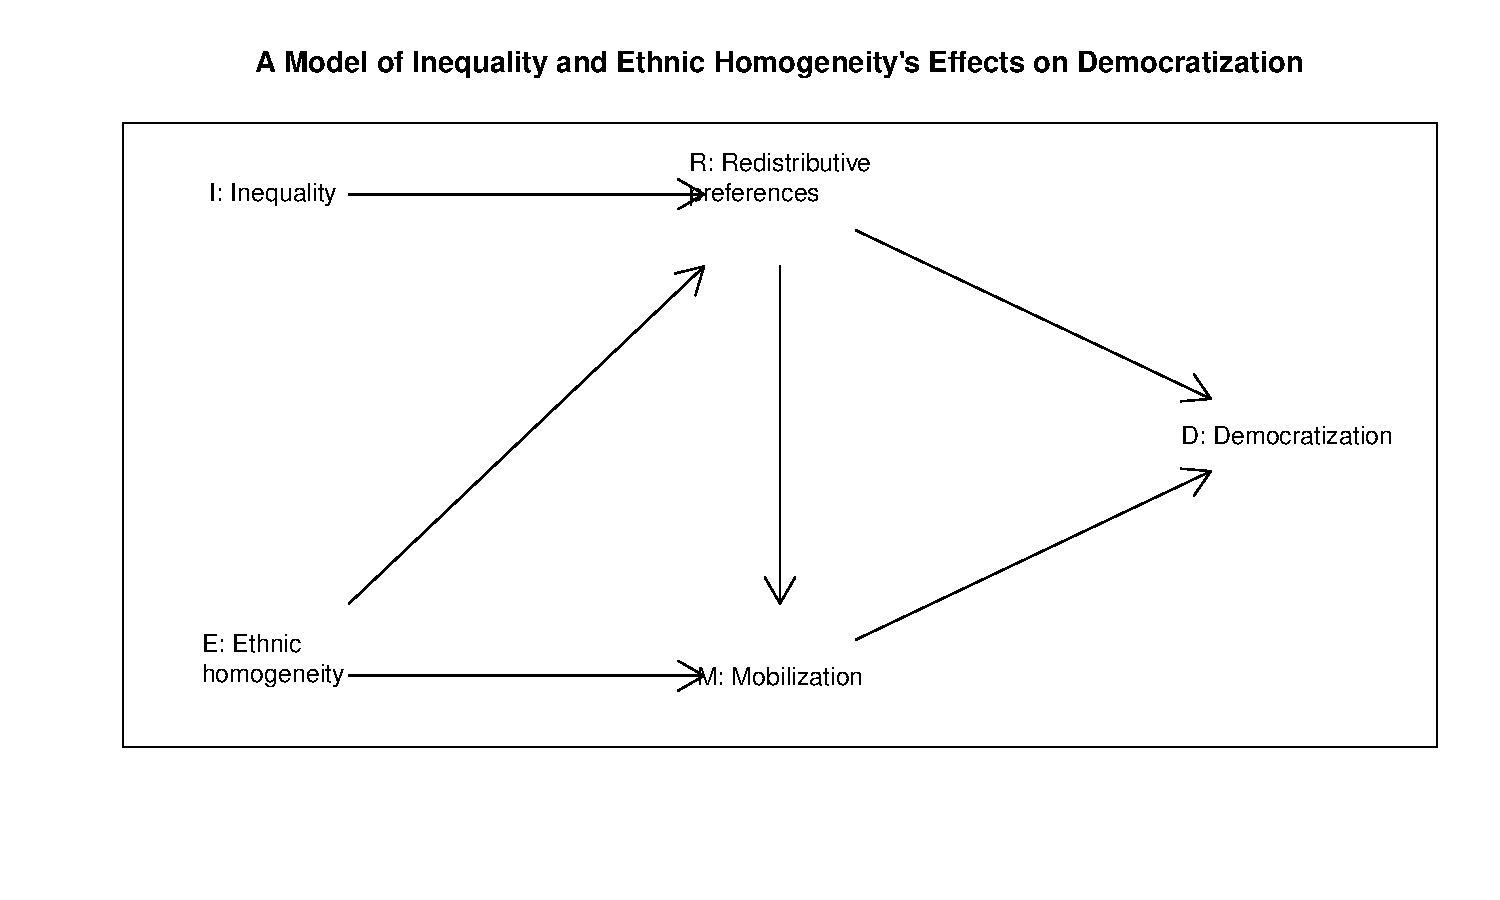
\includegraphics[width=.5\textwidth]{ii_files/figure-latex/lowercomplexdem-1} 

}

\caption{A model  from which multiple simpler models can be derived.}\label{fig:lowercomplexdem}
\end{figure}



\begin{figure}

{\centering 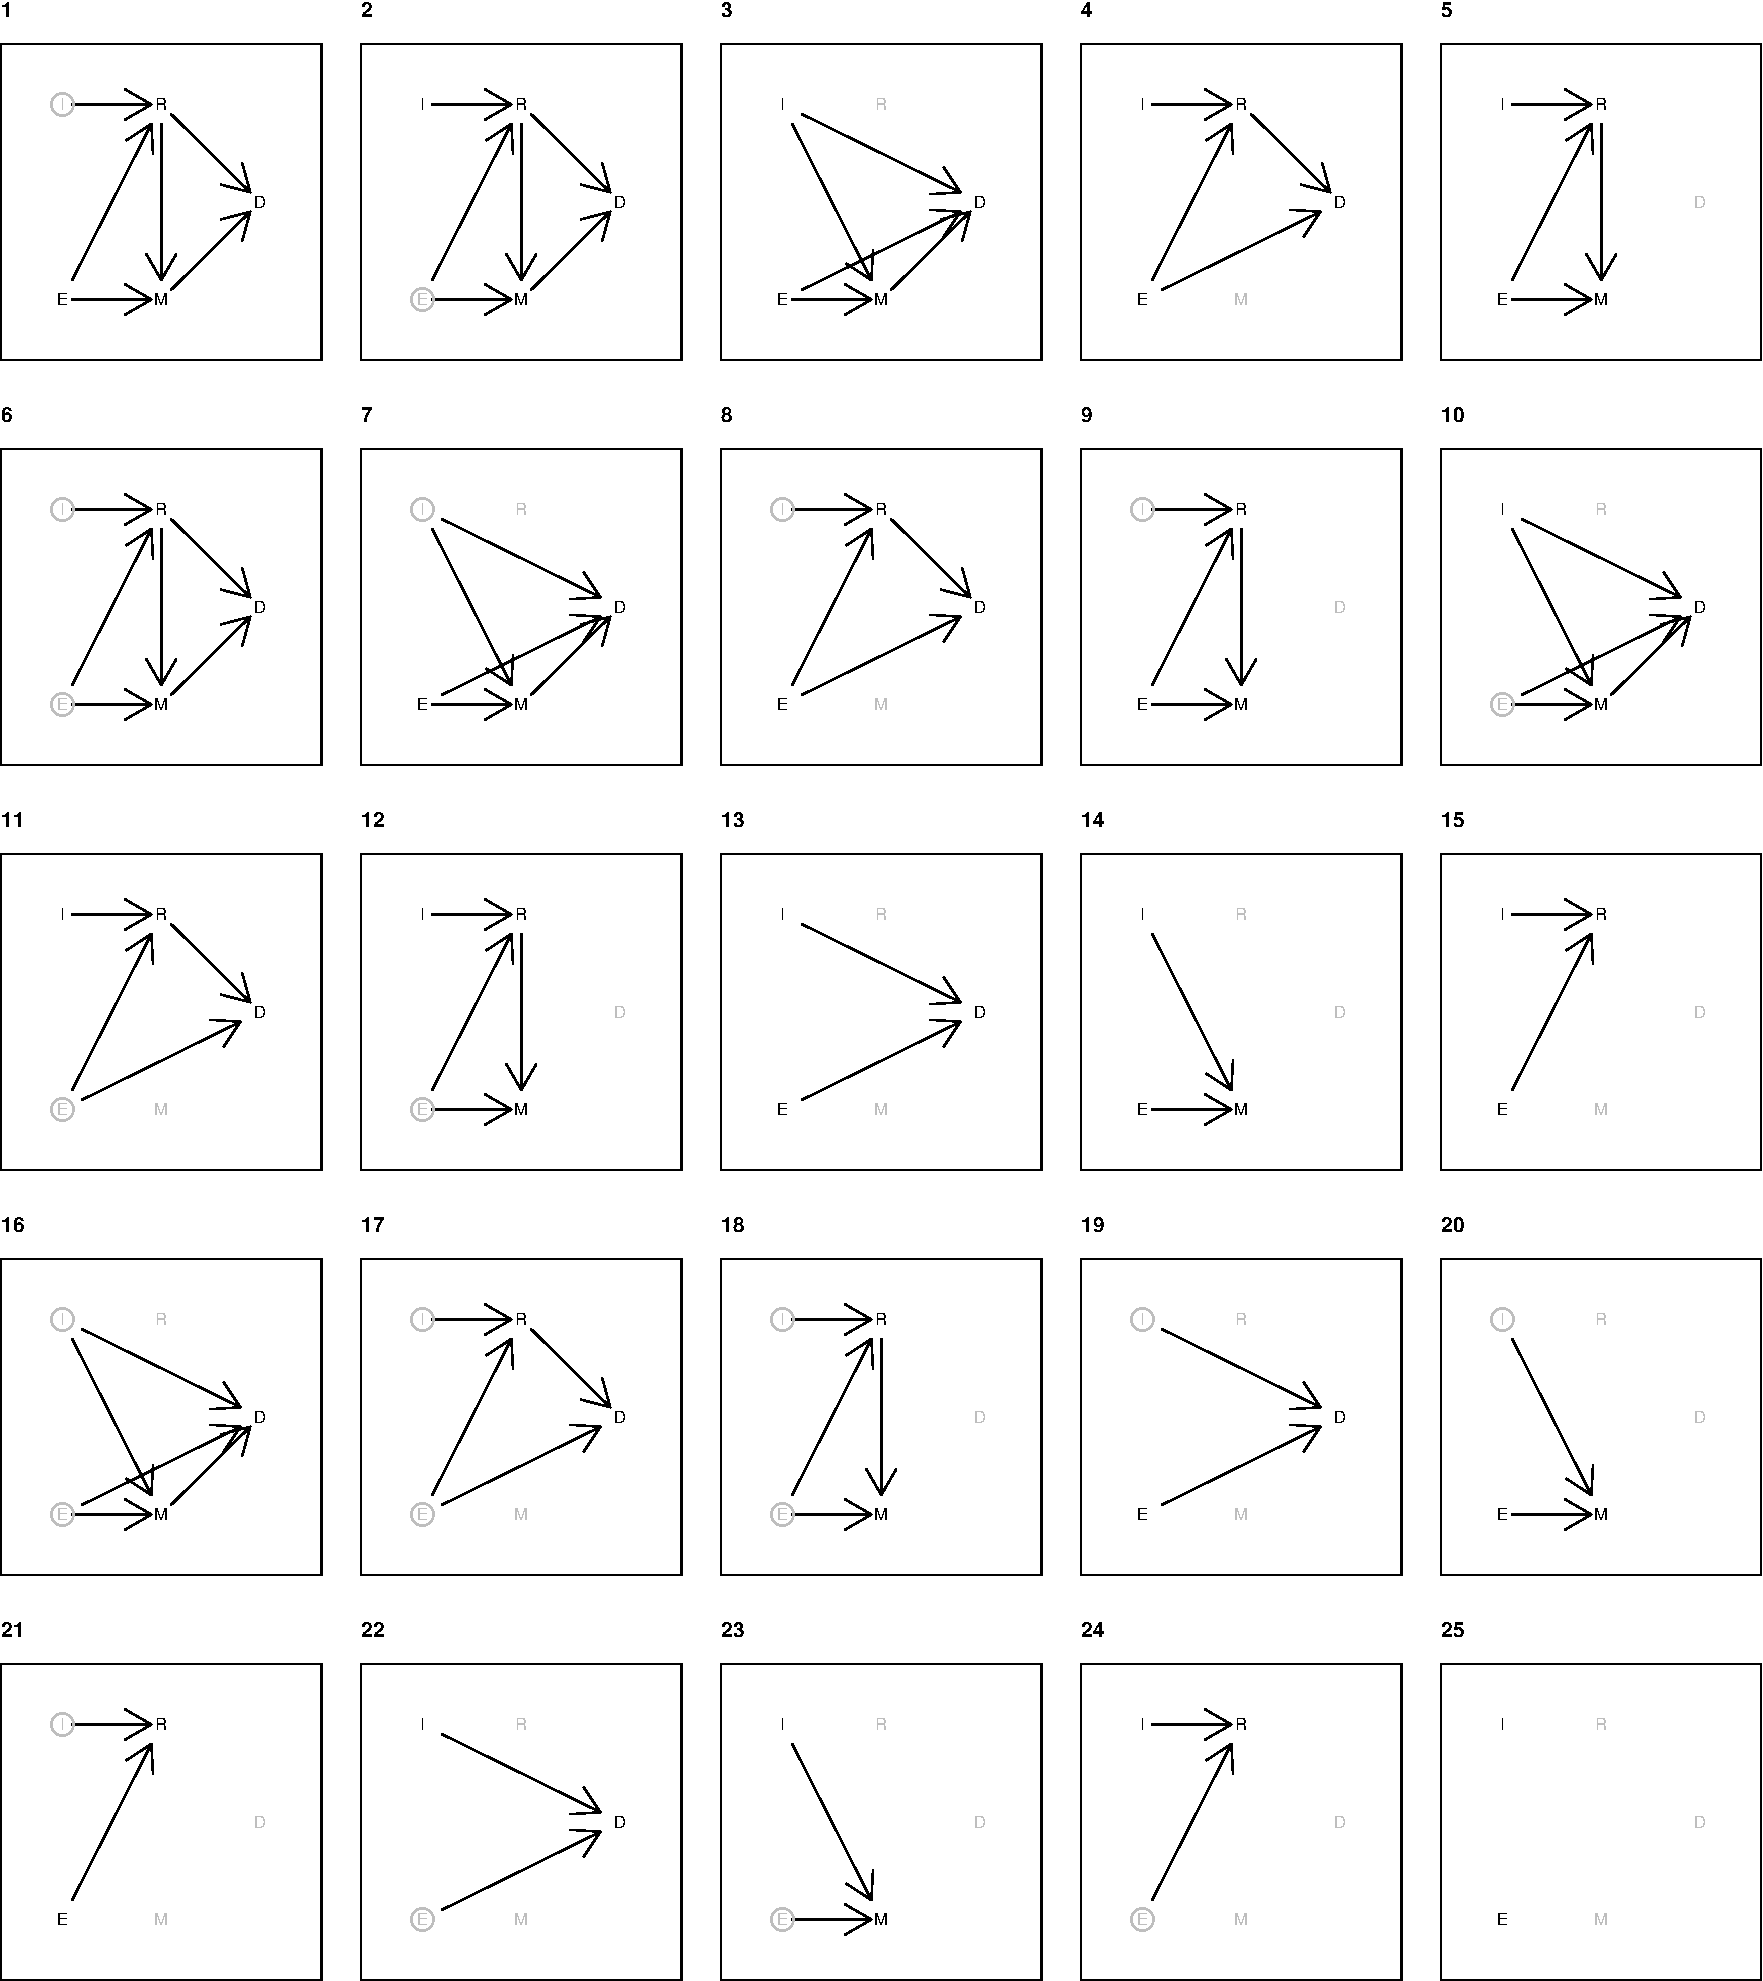
\includegraphics{ii_files/figure-latex/runningsubs-1} 

}

\caption{Simplifications of the model of Figure \ref{fig:lowercomplexdem}. Nodes that are eliminated are marked in grey; circles denote exogenous nodes that are replaced in subgraphs by unidentified variables. (A circled node pointing into two other nodes could equivalently be indicated as an undirected edge connecting the two.)}\label{fig:runningsubs}
\end{figure}

We can apply these principles to a model of any complexity. We illustrate a wider range of simplifications by starting with Figure \ref{fig:lowercomplexdem}. In Figure \ref{fig:runningsubs}, we show all permissible reductions of the more elaborate model. We can think of these reductions as the full set of simpler claims (involving at least two nodes) that can be derived from the original model. In each subgraph,

\begin{itemize}
\tightlist
\item
  we mark eliminated nodes in grey;
\item
  those nodes that are circled must be replaced with \(\theta\) terms; and
\item
  arrows represent the causal dependencies that must be preserved.
\end{itemize}

Note, for instance, that neither \(I\) (because it has a spouse) nor \(E\) (because it has multiple children) can be simply eliminated; each must be replaced with a \(\theta\) term. Also, the simplified graph with nodes missing can contain arrows that do not appear at all in the graph: eliminating \(R\), for instance, forces an arrow running from \(E\) to \(M\) (though that is there already) and another running from \(E\) to \(D\), as \(E\) must adopt \(R\)'s children. The simplest elimination is of \(Y\) itself since it does not encode any dependencies between other variables.

\hypertarget{conditioning-on-nodes}{%
\subsubsection{Conditioning on nodes}\label{conditioning-on-nodes}}

Another way to simpify a model is to condition on the value of a node. When we condition on a node, we are restricting the model in scope to situations in which that node's value is held constant. Doing so allows us to eliminate the node as well as all arrows pointing into it or out of it. Consider three different situations in which we might condition on a node:

\begin{itemize}
\tightlist
\item
  \emph{Exogenous, with multiple children.} In simplifying (a1) in Figure \ref{fig:elimrules}, we need to be sure we retain any dependence that \(X\) generates between \(W\) and \(Y\). However, recalling the rules of conditional independence on a graph (see Chapter \ref{models}), we know that \(W\) and \(Y\) are \emph{independent} conditional on \(X\). Put differently, if we restrict the analysis to contexts in which \(X\) takes on a constant value, the model implies that \(Y\) and \(W\) will be uncorrelated across cases. As fixing \(X\)'s value breaks the dependence between \(Y\) and \(W\), we can drop \(X\) (and the arrows pointing out of it) without having to represent that dependence.
\item
  \emph{Exogenous, with spouse.} In simplifying (b1) or (c1) in Figure \ref{fig:elimrules}, we need to account for the variation generated by \(X\). If we fix \(X\)'s value, however, then we eliminate this variation by assumption and do not need to continue to represent it (or the arrow pointing out of it) on the graph.
\item
  \emph{Endogenous.} When we condition on an endogenous node, we can eliminate the node as well the arrows pointing into and out of it. We, again, leverage relations of conditional independence here. If we start with model \(X \rightarrow M \rightarrow Y\) and we condition on the mediator, \(M\), we sever the link between \(Y\) and \(X\), rendering them conditionally independent of one another. We can thus remove \(M\), the arrow from \(X\) to \(M\), and the arrow from \(M\) to \(Y\). In the new model, with \(M\) fixed, \(Y\) will be entirely determined by the random disturbance \(\theta^{Y}\).
\end{itemize}

\hypertarget{retaining-probabilistic-relations}{%
\subsection{Retaining probabilistic relations}\label{retaining-probabilistic-relations}}

We have highlighted the graphical implications of node elimination or node conditioning but importantly the distribution over \(\theta\) also needs to be preserved faithfully in a move to a simpler model.

In sum, we can work with models that are simpler than our causal beliefs: we may believe a model to be true, but we can derive from it a sparser set of claims. There may be intervening causal steps or features of context that we believe matter, but that are not of interest for a particular line of inquiry. While these can be removed, we nonetheless have to make sure that their \emph{implications} for the relations remaining in the model are not lost. Understanding the rules of reduction allow us to undertake an important task: checking which simpler claims are and are not consistent with our full belief set.

\hypertarget{conc2}{%
\section{Conclusion}\label{conc2}}

In this chapter, we have shown how we can inscribe causal beliefs, rooted in the potential outcomes framework, into a causal model. In doing so, we have now set out the foundations of the book's analytic framework. Causal models are both the starting point for analysis in this framework and the object about which we seek to learn. Before moving on to build on this foundation, we aim in the next chapter to offer further guidance by example on the construction of causal models, by illustrating how a set of substantive social scientific arguments from the literature can be represented in causal model form.

\newpage

\hypertarget{chapter-appendix}{%
\section{Chapter Appendix}\label{chapter-appendix}}

\hypertarget{steps-for-constructing-causal-models}{%
\subsection{Steps for constructing causal models}\label{steps-for-constructing-causal-models}}

\begin{headerbox}

\begin{center}
\textbf{Steps for constructing causal models}

\end{center}

\begin{enumerate}
\def\labelenumi{\arabic{enumi}.}
\tightlist
\item
  Identify a set of variables in a domain of interest. These become the nodes of the model.
\end{enumerate}

\begin{itemize}
\tightlist
\item
  Specify the range of each node: is it continuous or discrete?
\item
  Each node should have an associated \(\theta\) term representing unspecified other influences (not necessarily graphed)
\end{itemize}

\begin{enumerate}
\def\labelenumi{\arabic{enumi}.}
\setcounter{enumi}{1}
\tightlist
\item
  Draw a causal graph (DAG) representing beliefs about causal dependencies among these nodes
\end{enumerate}

\begin{itemize}
\tightlist
\item
  Include arrows for direct effects only
\item
  Arrows indicate \emph{possible} causal effects
\item
  The absence of an arrow between two nodes indicates a belief of \emph{no} direct causal relationship between them
\item
  Ensure that the graph captures all correlations among nodes. This means that either (a) any common cause of two or more nodes is included on the graph (with implications for Step 1) or (b) correlated nodes are connected with a dashed or curved, undirected edge.
\end{itemize}

\begin{enumerate}
\def\labelenumi{\arabic{enumi}.}
\setcounter{enumi}{2}
\tightlist
\item
  Write down one causal function for each endogenous node
\end{enumerate}

\begin{itemize}
\tightlist
\item
  Each node's function must include all nodes directly pointing into it on the graph as well as the \(\theta\) terms
\item
  Functions may express arbitrary amounts of uncertainty about causal relations
\end{itemize}

\begin{enumerate}
\def\labelenumi{\arabic{enumi}.}
\setcounter{enumi}{3}
\tightlist
\item
  State probabilistic beliefs about the distributions of the \(\theta\)s.
\end{enumerate}

\begin{itemize}
\tightlist
\item
  How common or likely to do we think different values of the exogenous nodes are?
\item
  Are they independently distributed? If in step 2 you drew an undirected edge between nodes then you believe that the connected nodes are not independently distributed.
\end{itemize}

\end{headerbox}

\hypertarget{model-construction-in-code}{%
\subsection{Model construction in code}\label{model-construction-in-code}}

Our \texttt{CausalQueries} package provides a set of functions to implement all of these steps concisely for \emph{binary} models -- models in which all nodes are dichotomous.

\begin{Shaded}
\begin{Highlighting}[]
\CommentTok{\# Steps 1 and 2 }
\CommentTok{\# We define a model with three binary nodes and }
\CommentTok{\# specified edges between them:}
\NormalTok{model }\OtherTok{\textless{}{-}} \FunctionTok{make\_model}\NormalTok{(}\StringTok{"X {-}\textgreater{} M {-}\textgreater{} Y"}\NormalTok{)}

\CommentTok{\# Functional forms are unrestricted. Restrictions can }
\CommentTok{\# be added. Here we impose monotonicity at each step }
\CommentTok{\# by removing one type for M and one for Y}
\NormalTok{model }\OtherTok{\textless{}{-}} \FunctionTok{set\_restrictions}\NormalTok{(model, }\AttributeTok{labels =} \FunctionTok{list}\NormalTok{(}\AttributeTok{M =} \StringTok{"10"}\NormalTok{, }\AttributeTok{Y=}\StringTok{"10"}\NormalTok{))}

\CommentTok{\# Step 4}
\CommentTok{\# Set priors over the distribution of (remaining) causal types.}
\CommentTok{\# Here we set "jeffreys priors"}
\NormalTok{model }\OtherTok{\textless{}{-}} \FunctionTok{set\_priors}\NormalTok{(model, }\AttributeTok{distribution =} \StringTok{"jeffreys"}\NormalTok{)}

\CommentTok{\# We now have a model defined as an R object. }
\CommentTok{\# Later we will update  and query this model}
\end{Highlighting}
\end{Shaded}

These steps are enough to fully describe a binary causal model. Later in this book we will see how we can ask questions of a model like this but also how to use data to train it.

\hypertarget{rules-for-moving-between-levels}{%
\subsection{Rules for moving between levels}\label{rules-for-moving-between-levels}}

\begin{headerbox}

\begin{center}
\textbf{Rules for moving between levels}

\end{center}

\emph{Moving down levels}:

All (conditional) independencies represented in a higher-level model must be preserved in the lower-level model.

When we disaggregate or add nodes to a model, new conditional independencies can be generated. But any variables that are independent or conditionally independent (given a third variable) in the higher-level model must also be independent or conditionally independent in the lower-level model.

\emph{Moving up levels}:

We can move up levels by eliminating an exogenous node, eliminating an endogenous node, or conditioning on a node. When we eliminate a node from a model, we must preserve any variation and dependencies that it generates:

\begin{enumerate}
\def\labelenumi{\arabic{enumi}.}
\tightlist
\item
  When eliminating an endogenous node, that node's parents adopt (become direct causes of) that node's children.
\item
  When eliminating an exogenous node, we must usually replace it with a \(\theta\) term. If the node has more than one child, it must be replaced with a \(\theta\) term pointing into both children (or an undirected edge connecting them) to preserve the dependency between its children. If the node has a spouse, the eliminated node's variation must also be preserved using a \(\theta\) term. Where the spouse is (already) a \(\theta\) term with no other children, \(\theta\) terms can be combined.\\
\item
  Since conditioning on a node ``blocks'' the path through which it connects its children, we can simply eliminate the node and the arrows between it and its children.
\item
  An exogenous node with no spouse and only one child can be simply eliminated.
\end{enumerate}

\end{headerbox}

\hypertarget{reading-conditional-independence-from-a-graph}{%
\subsection{Reading conditional independence from a graph}\label{reading-conditional-independence-from-a-graph}}

We illustrate how to identify the relations of conditional independence between \(A\) and \(D\) in Figure \ref{fig:exercise}.

\begin{figure}

{\centering 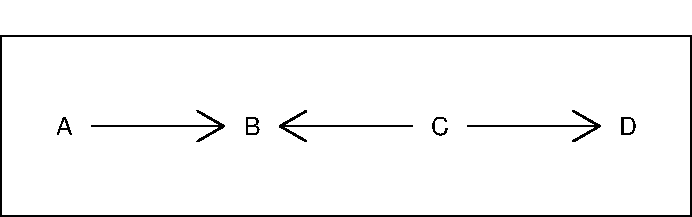
\includegraphics[width=0.8\linewidth]{ii_files/figure-latex/exercise-1} 

}

\caption{\label{fig:CItest} An exercise: $A$ and $D$ are conditionally independent, given which other node(s)?}\label{fig:exercise}
\end{figure}

Are A and D independent:

\begin{itemize}
\tightlist
\item
  unconditionally?
\end{itemize}

Yes. \(B\) is a collider, and information does not flow across a collider if the value of the collider node or its consequences is not known. Since no information can flow between \(A\) and \(C\), no information can flow between \(A\) and \(D\) simply because any such flow would have to run through \(C\).

\begin{itemize}
\tightlist
\item
  if you condition on \(B\)?
\end{itemize}

No.~Conditioning on a collider opens the flow of information across the incoming paths. Now, information flows between \(A\) and \(C\). And since information flows between \(C\) and \(D\), \(A\) and \(D\) are now also connected by an unbroken path. While \(A\) and \(D\) were independent when we conditioned on nothing, they cease to be independent when we condition on \(B\).

\begin{itemize}
\tightlist
\item
  if you condition on \(C\)?
\end{itemize}

Yes. Conditioning on \(C\), in fact, has no effect on the situation. Doing so cuts off \(B\) from \(D\), but this is irrelevant to the \(A\)-\(D\) relationship since the flow between \(A\) and \(D\) was already blocked at \(B\), an unobserved collider.

\begin{itemize}
\tightlist
\item
  if you condition on \(B\) and \(C\)?
\end{itemize}

Yes. Now we are doing two, countervailing things at once. While conditioning on \(B\) opens the path connecting \(A\) and \(D\), conditioning on \(C\) closes it again, leaving \(A\) and \(D\) conditionally independent.

Analyzing a causal graph for relations of independence represents one payoff to formally encoding our beliefs about the world in a causal model. We are, in essence, drawing out implications of those beliefs: given what we believe about a set of direct causal relations (the arrows on the graph), what must this logically imply about other dependencies and independencies on the graph, conditional on having observed some particular set of nodes? We show in a later chapter how these implications can be deployed to guide research design, by indicating which parts of a causal system are potentially informative about other parts that may be of interest.

\hypertarget{illustratemodels}{%
\chapter{Illustrating Causal Models}\label{illustratemodels}}

\begin{headerbox}
We use three arguments from published political science research to illustrate how to represent theoretical ideas as structural causal models.

\end{headerbox}

In this short chapter, we provide more of a sense of how we can encode prior knowledge in a causal model by asking how we might construct models in light of extant scholarly works. We undertake this exercise by drawing on three well-known publications in comparative politics and international relations: Paul Pierson's seminal book on welfare-state retrenchment \citep{pierson1994dismantling}; Elizabeth Saunders' research on leaders' choice of military intervention strategies \citep{saunders2011leaders}; and Przeworski and Limongi's work on democratic survival \citep{przeworski1997modernization}, an instructive counterpoint to Boix's \citep{boix2003democracy} argument about a related dependent variable. For each, we represent the causal knowledge that we might plausibly think we take away from the work in question in the form of a causal model.

Readers might represent these knowledge bases differently; our aim here is only to illustrate how causal models are constructed, rather than to defend a particular representation (much less the works in question) as accurate.

For each exercise below, we focus on a specific argument in the literature in order to fix in place a relatively clear set of background causal beliefs and simplify the exposition. We emphasize, however, that \emph{in general} a causal model should be thought of as a representation of our state of knowledge or beliefs about causal relations within a domain, rather than as a representation of a specific argument. Suppose, for instance, that we are interested in testing a specific argument in which \(X\) affects \(Y\) through the mediator \(M\). In constructing a causal model to guide our empirical analysis, we cannot simply draw that argument in DAG form (\(X \rightarrow M \rightarrow Y\)) and leave it at that. In line with the principles relating to conditional independence outlined in Chapter \ref{models}, we must consult our beliefs about this causal domain in a broader sense. For instance, given what we know about the domain from prior observations or studies, is it plausible that \(X\) could affect \(Y\) through a pathway that does not go through \(M\)? If we believe it is possible, then we must also draw a direct \(X \rightarrow Y\) arrow, or our causal model will steer us wrong --- even if our primary aim is to examine the pathway through \(M\). Otherwise, our DAG will contain a relation of conditional independence (\(X\) being conditionally independent of \(Y\) given \(M\)) that we do not believe holds. Thus, while we draw on specific works in the illustrations in this chapter, we urge readers to remember that in practice one would want to characterize a broader prior knowledge base in relation to a causal domain in generating a causal model.

We aim to illuminate a number of features of causal models and their construction with these exercises. The examples that we work through variously illustrate how graphs capture beliefs about relations of conditional independence; the potential causal complexity embedded in the causal structures implied by common social-scientific arguments; and the elements of a causal model that cannot be read from a graph. For each work, we discuss both a parametric rendering of the causal functions and a non-parametric formulation built on nodal types.

\hypertarget{welfare-state-reform}{%
\section{Welfare state reform}\label{welfare-state-reform}}

The argument in Pierson's 1994 book \emph{Dismantling the Welfare State?} challenged prior notions of post-1980 welfare-state retrenchment in OECD countries as a process driven primarily by socioeconomic pressures (slowed growth, rising unemployment, rising deficits, aging populations) and the rise of market-conservative ideologies (embodied for instance by the ascendance of Thatcher and Reagan). Pierson argues that socioeconomic and ideological forces put retrenchment on the policy agenda, but do not ensure its enactment because retrenchment is a politically perilous process of imposing losses on large segments of the electorate. Governments will only impose such losses if they can do so in ways that allow them avoid blame for doing so---by, for instance, making the losses hard to perceive or the responsibility for them difficult to trace. These blame-avoidance opportunities are themselves conditioned by the particular social-program structures that governments inherit.

\begin{figure}

{\centering 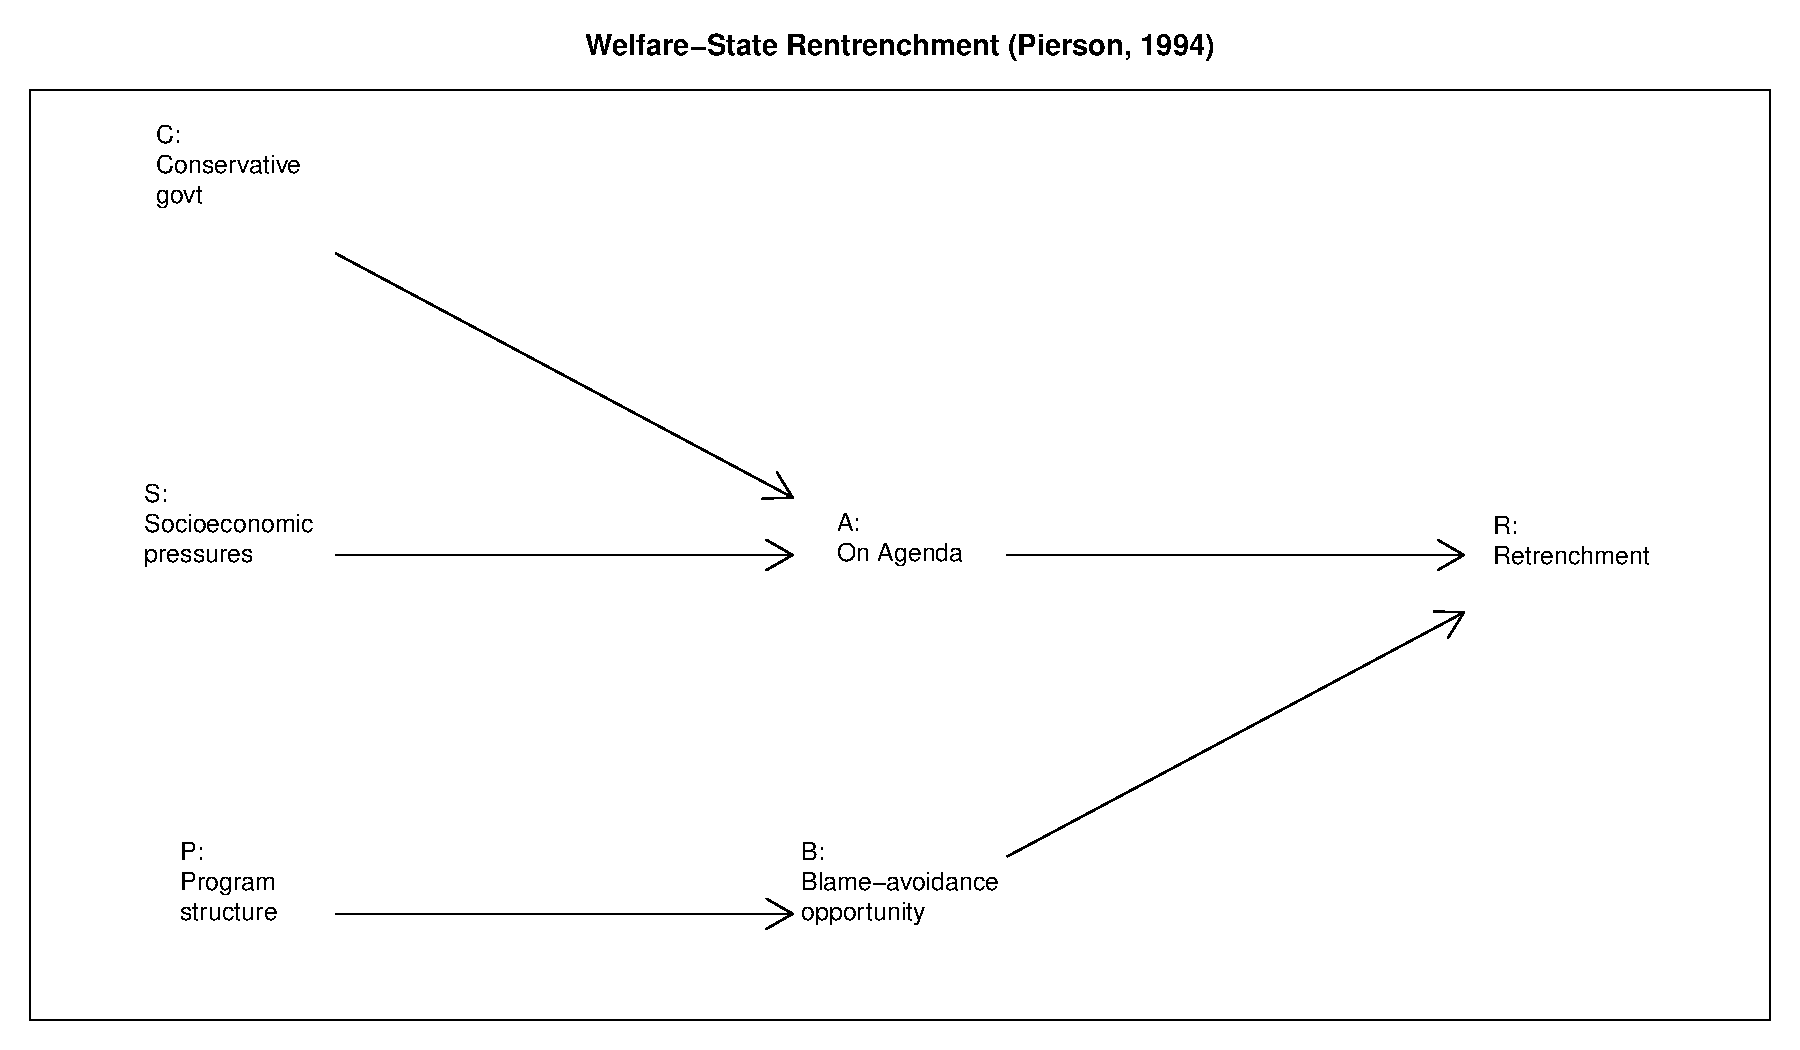
\includegraphics[width=.7\textwidth]{ii_files/figure-latex/pierson-1} 

}

\caption{A graphical representation of Pierson (1994).}\label{fig:pierson}
\end{figure}

While the argument has many more specific features (e.g., different program-structural factors that matter, various potential strategies of blame-avoidance), its essential components can be captured with a relatively simple causal model. We propose such a model in graphical form in Figure \ref{fig:pierson}. Here, the outcome of retrenchment (\(R\)) hinges on whether retrenchment makes it onto the agenda (\(A\)) and on whether blame-avoidance strategies are available to governments (\(B\)). Retrenchment emerges on the policy agenda as a consequence of both socioeconomic developments (\(S\)) and the ascendance of ideologically conservative political actors (\(C\)). Inherited program structures (\(P\)), meanwhile, determine the availability of blame-avoidance strategies. To avoid cluttering the graph, we do not represent the \(\theta\) terms, but it is implied that every node on this graph has a \(\theta\) node pointing into it.

A few features of this graph warrant attention. As we have discussed, it is the omitted arrows in any causal graph that imply the strongest statements. The graph implies that \(C\), \(S\), and \(P\)---which are neither connected along a directed path nor downstream from a common cause---are independent of one another. This implies, for instance, that whether conservatives govern is independent of whether program structures will allow for blame-free retrenchment. Thus, as Pierson argues, a Reagan or Thatcher can come to power but nonetheless run up against an opportunity structure that would make retrenchment politically perilous. Given the absence of bidirectional arrows indicating confounding, the graph similarly implies that the nodal types for all nodes are independent of one another.

Further, this graph represents the belief that any effect of program structures on retrenchment \emph{must} run through their effects on blame-avoidance opportunities. One could imagine relaxing this restriction by, for instance, drawing an arrow from \(P\) to \(A\): program structures might additionally affect retrenchment in other ways, such as by conditioning the fiscal costliness of the welfare state and thus helping to determine whether reform makes it onto the agenda. If the current state of knowledge suggested that program structures could affect retrenchment via a pathway other than blame-avoidance opportunities, then we would indeed want to include a direct \(P \rightarrow A\) arrow.

Where two variables \emph{are} connected by an arrow, moreover, this does not imply that a causal effect will always operate. Consider, for instance, the arrow pointing from \(A\) to \(R\). The fact that \(A\) sometimes affects \(R\) and sometimes does not is, in fact, central to Pierson's argument: conservatives and socioeconomic pressures forcing retrenchment on the agenda will \emph{not} generate retrenchment if blame-avoidance opportunities are absent.

The graph also reflects a choice about where to begin. We could, of course, construct a causal account of how conservatives come to power, how socioeconomic pressures arise, or why programs were originally designed as they were. Yet it is perfectly permissible for us to bracket these antecedents and start the model with \(C\), \(S\), and \(T\), as long as we do not believe that these variables have any antecedents in common. If they do have common causes, then this correlation should be captured in the DAG.\footnote{In DAG syntax, this correlation can be captured by placing the common cause(s) explicitly on the graph or by drawing a dashed line between the correlated nodes, leaving the source of the correlation unspecified.}

The DAG itself tells us about the possible direct causal dependencies but is silent on the ranges of and functional relations among the variables. How might we express these? With three endogenous variables, we need three functions indicating how their values are determined. Moreover, every variable pointing directly into another variable must be part of that second variable's function.

Let us assume that all variables (including the implied \(\theta\) terms) are binary, with each condition either absent or present.

One option would be to take a parameteric approach and imagine specific functions connecting parents to children, with \(\theta\) terms representing exogenous ``noise.'' For instance, we can capture quite a lot of Pierson's theoretical logic with the following quite simple functional equations:

\begin{itemize}
\tightlist
\item
  \(A=CS\theta^C\), capturing the idea that retrenchment makes it on the agenda only if conservatives are in power \emph{and} socioeconomic pressures are high.
\item
  \(B=P\theta^P\), implying that blame-avoidance opportunities arise only when program structures take a particular form.
\item
  \(R=AB\theta^R\), implying that retrenchment will occur only if it is on the agenda and blame-avoidance opportunities are present.
\end{itemize}

In each equation, the \(\theta\) term allows for exogenous forces that might block the outcome from occurring. In the last functional equation, for instance, retrenchment will only occur if retrenchment is on the agenda and blame-avoidance opportunities are present, but even if both are present, the effect on retrenchment also hinges on the value of \(\theta^R\). When \(\theta^R=1\), the \(AB\) combination has a positive causal effect on retrenchment. When \(\theta^R=0\), \(AB\) has no causal effect: retrenchment will not occur regardless of the presence of \(AB\). We can think of \(\theta^R\) as capturing a collection of features of a case's context that might render the case susceptible or not susceptible to an \(AB\) causal effect. For instance, Pierson's analysis suggests that a polity's institutional structure might widely diffuse veto power such that stakeholders can block reform even when retrenchment is on the agenda and could be pursued without electoral losses. We could think of such a case as having a \(\theta^R\) value of 0, implying that \(AB\) has no causal effect. A \(\theta^R=1\) case, with a positive effect, would be one in which the government has the institutional capacity to enact reforms that it has the political will to pursue.

Alternatively, we could take a non-parameteric approach, as we generally do in the remainder of this book. In a non-parametric setup, each node's \(\theta\) term captures that node's nodal type. Each value of a \(\theta\) term's range represents a possible way in which the node might respond to its parents. We would define \(\theta^A\) as taking on one of 16 values (16 types, given 2 parent nodes); \(\theta^B\) as taking on on one of four values; and \(\theta^R\) as taking on one of 16 values; with \(\theta^C\) and \(\theta^S\) each taking on one of two values.

Then choices on the probability distributions fully reflect the ways these variables relate to each other. Note that the parametric argument given above can be thought of as a special case of the non-parametric representation with all probability mass placed on a small set of possible nodal types. Thus the central thrust of Pierson's argument could then be represented in nodal-type form as:

\begin{itemize}
\tightlist
\item
  \(\theta^A=\theta^A_{0001}\)
\item
  \(\theta^B=\theta^B_{01}\)
\item
  \(\theta^R=\theta^R_{0001}\).
\end{itemize}

In practice, however we would allow for a richer probability \emph{distribution} over each \(\theta\), representing beliefs over the assignment process or causal relations operating at each node. Beliefs about the distribution of exogenous conditions would be captured in distributions over the values of \(\theta^C, \theta^S\), and \(\theta^P\). How we handle distributions over \(\theta^A, \theta^B\), and \(\theta^R\) depends on the degree of confidence that we want to express in Pierson's argument. To represent the belief that Pierson's argument is correct with certainty and operates in uniform, deterministic fashion across units, we would simply have degenerate distributions for \(\theta^A, \theta^B\), and \(\theta^R\), with a probability of 1.0 placed on the respective nodal types shown above. To capture uncertainty about the functional relations on any graph or if we believe that there is some heterogeneity of effects across units we would disperse probability density across types for each \(\theta\). For instance, for \(\theta^R\) we might want to put some weight on \(\theta^R_{0011}\) (blame-avoidance opportunities alone are enough to generate retrenchment), \(\theta^R_{0101}\) (conservative leaders alone are enough), \(\theta^R_{0111}\) (either is enough), and \(\theta^R_{0000}\) (retrenchment will not happen even when both conditions are present), while perhaps putting greatest weight on \(\theta^R_{0001}\).\footnote{In notation that we use later, these beliefs would be represented with a \(\lambda^R\) vector.}

\hypertarget{military-interventions}{%
\section{Military Interventions}\label{military-interventions}}

\citet{saunders2011leaders} asks why, when intervening militarily abroad, do leaders sometimes seek to transform the \emph{domestic} political institutions of the states they target but sometimes seek only to shape the states' \emph{external} behaviors.

Saunders' central explanatory variable is the nature of leaders' causal beliefs about security threats. When leaders are ``internally focused,'' they believe that threats in the international arena derive from the internal characteristics of other states. Leaders who are ``externally focused,'' by contrast, understand threats as emerging strictly from other states' foreign and security policies.

These basic worldviews, in turn, affect the cost-benefit calculations leaders make about intervention strategies---in particular, about whether to try to transform the internal institutions of a target state---via two mechanisms. First, an internal focus (as opposed to an external focus) affects leaders' perceptions of the likely security gains from a transformative intervention strategy. Second, internal vs.~external focus affects the kinds of strategic capabilities in which leaders invest over time (do they invest in the kinds of capabilities suited to internal transformation?); and those investments in turn affect the costliness and likelihood of success of alternative intervention strategies. Calculations about the relative costs and benefits of different strategies then shape the choice between a transformative and non-transformative approach to intervention.

At the same time, leaders can only choose a transformative strategy if they decide to intervene at all. The decision about whether to intervene depends, in turn, on at least two kinds of considerations. The first is about fit: a leader is more likely to intervene against a target when the nature of the dispute makes the leader's preferred strategy appear feasible in a given situation. Second, Saunders allows that forces outside the logic of her main argument might also affect the likelihood of intervention: in particular, leaders may be pushed to intervene by international or domestic audiences.

Figure \ref{fig:DAGSaunders} depicts the causal dependencies in Saunders' argument in DAG form (again, with all \(\theta\) terms implied). Working from left to right, we see that whether or not leaders are ``internally focused'' (\(F\)) affects the expected net relative benefits of transformation (\(B\)), both via a direct pathway and via an indirect pathway running through investments in transformative capacities (\(T\)). Characteristics of a given dispute or target state (\(D\)) likewise influence the benefits of transformation (\(B\)). The decision about whether to intervene (\(I\)) is then a function of three factors: internal focus (\(F\)), the expected relative net benefits of transformation (\(B\)), and audience pressures (\(A\)). Finally, the choice of whether to pursue a transformative strategy (\(S\)) is a function of whether or not intervention occurs at all (\(I\)), and of cost-benefit comparisons between the two strategies (\(B\)).

\begin{figure}

{\centering 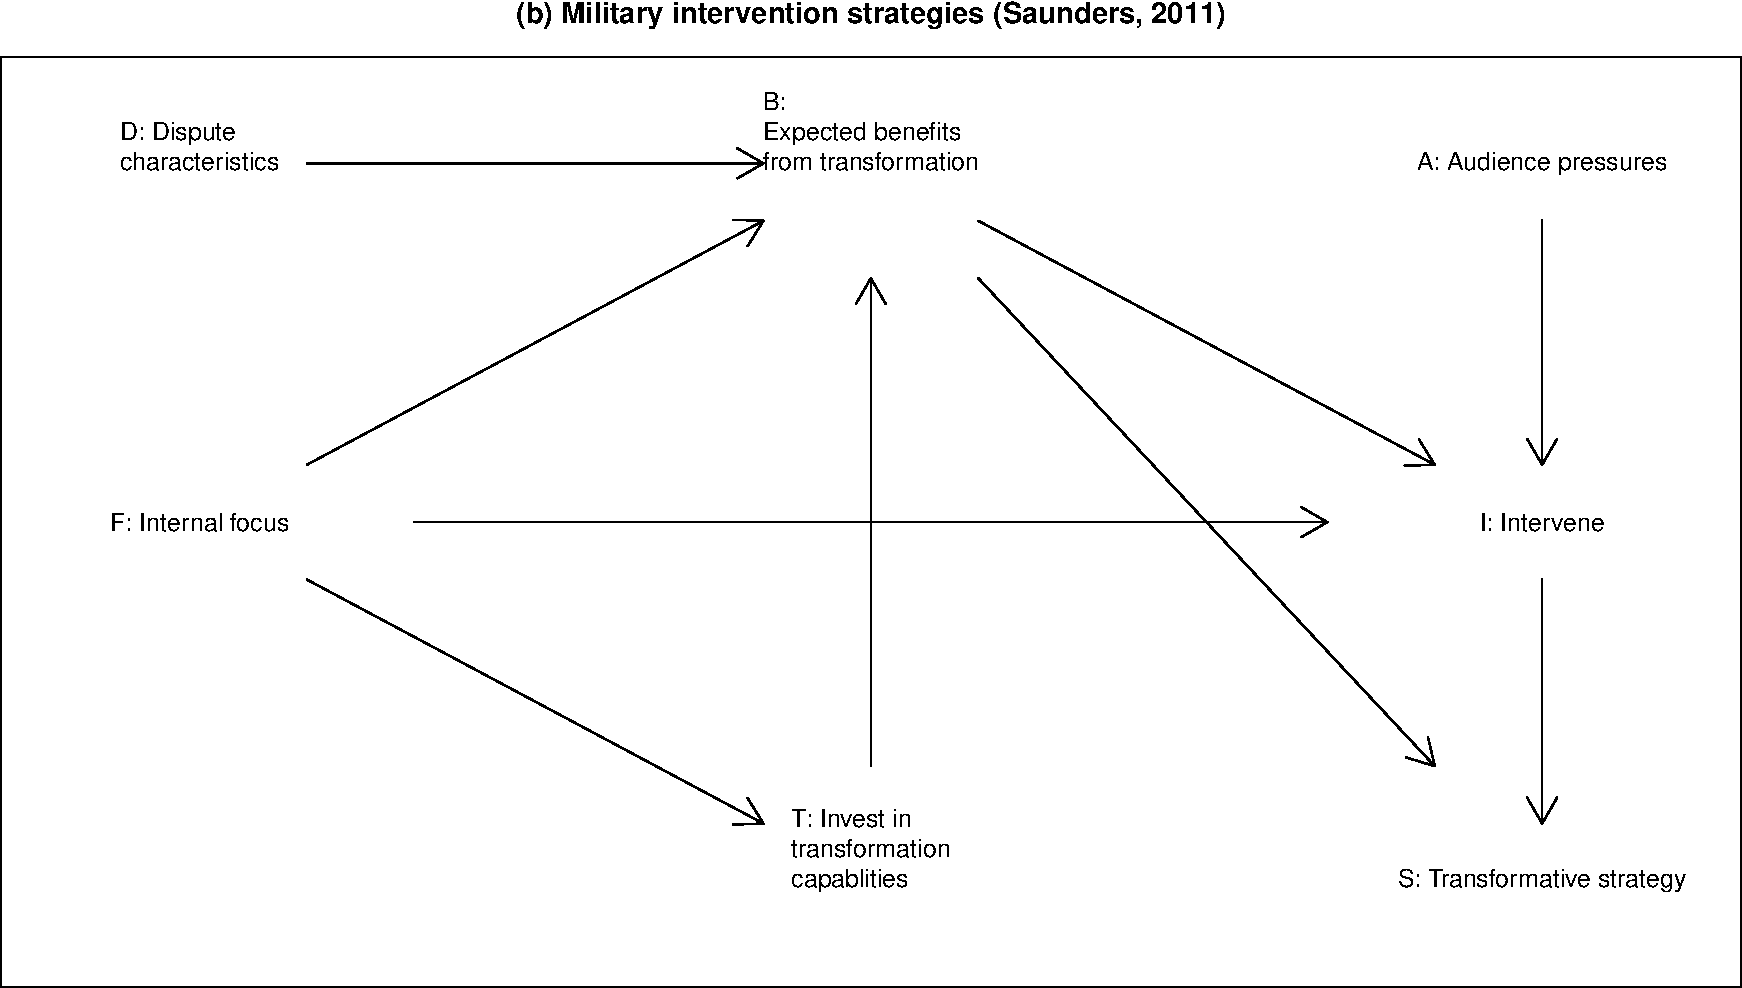
\includegraphics[width=.7\textwidth]{ii_files/figure-latex/saunders-1} 

}

\caption{\label{fig:DAGSaunders} A graphical representation of Saunders' (2011) argument.}\label{fig:saunders}
\end{figure}

This DAG illustrates how readily causal graphs can depict the multiple pathways through which a given variable might affect another variable, as with the multiple pathways linking \(F\) to \(I\) and \(B\) (and, thus, all of its causes) to \(S\). In fact, this graphical representation of the dependencies in some ways throws the multiplicity of pathways into even sharper relief than does a narrative exposition of the argument. For instance, Saunders draws explicit attention to how causal beliefs operate on expected net benefits via both a direct and indirect pathway, both of which are parts of an indirect pathway from \(F\) to the outcomes of interest, \(I\) and \(S\). What is a bit easier to miss without formalization is that \(F\) also acts \emph{directly} on the choice to intervene as part of the feasibility logic: when leaders assess whether their generally preferred strategy would be feasible if deployed against a particular target, the generally preferred strategy is itself a product of their causal beliefs. The DAG also makes helpfully explicit that the two main outcomes of interest---the choice about whether to intervene and the choice about how---are not just shaped by some of the same causes but are themselves causally linked, with the latter depending on the former.

Omitted links are also notable. For instance, the lack of an arrow between \(D\) and \(A\) suggests that features of the dispute that affect feasibility have no effect on audience pressures. If we instead believed there could be other connections---for instance, that audiences take feasibility into account in demanding intervention---then we would want to include a \(D \rightarrow A\) arrow.

Turning to variable ranges and functional equations, it is not hard to see how one might readily capture Saunders' logic in a fairly straightforward set-theoretic manner. All variables except \(S\) could be treated as binary with, for instance, \(F=1\) representing internally focused causal beliefs, \(T=1\) representing investments in transformative capabilities, \(B=1\) representing expectations that transformation will be more net beneficial than non-transformation, \(D=1\) meaning that a dispute has characteristics that make transformation a feasible strategy, and so on. Although there are two strategies, we in fact need three values for \(S\) because it must be defined for all values of the other variables---i.e., it must take on a distinct categorical value if there is no intervention at all. We could then define functions, such as:

\begin{itemize}
\tightlist
\item
  \(B=FTD\), implying that transformation will only be perceived to be net beneficial in a case if and only if the leader has internally focused causal beliefs, the government is prepared for a transformative strategy, and the dispute has characteristics that make transformation feasible.
\item
  \(I=(1-|B-F|)+(1-(1-|B-F|))A\), implying that intervention can occur under (and only under) either of two alternative sets of conditions: if the generally preferred strategy and the more net-beneficial strategy in a given case are the same (i.e., such that \(B-F=0\)) or, when this alignment is absent (i.e., such that \(|B-F|=0\)), where audiences pressure a leader to intervene.
\end{itemize}

As illustrated in the Pierson example, in a non-parametric framework, each parametric functional equation represents one nodal type for the relevant \(\theta\). For instance, though we spare the reader the complexities of the corresponding subscript notation, there is a single value of \(\theta^B\) under which the conditions \(F=1, P=1,\) and \(T=1\) generate \(B=1\), and we get \(B=0\) otherwise. Likewise, there exists a single value of \(\theta^I\) under which \(B=1, F=1\) and \(B=0, F=0\) produce \(I=1\), for either value of \(A\); and \(A\) has a positive effect on \(I\) whenever \(B \neq F\). To work with this model, we would specify a probability distribution over all possible nodal types for each node on the graph.

This example also nicely illustrates how much potential causal complexity a moderately intricate argument and causal graph implies. The number of \emph{possible} nodal types at each node depends on how many parents that node has. Looking at the endogenous nodes here, we have one node with one parent (\(T\)), implying 4 nodal types; one node with two parents (\(S\)), implying 16 nodal types; and two nodes with 3 parents (\(B\) and \(I\)), implying 256 nodal types each. If we now conceptualize the set of possible ``causal types'' as containing all distinct combinations of nodal types---all ways in which a case might behave across all of its nodes (see Chapter \ref{models})---then this graph implies about 4 million different ways in which the values of exogenous nodes (\(D\), \(F\), and \(A\)) might jointly produce patterns of outcomes. Saunders' argument effectively represents one of these 4 million possible sets of relations.

The framework that we outline in this book allows for updating on arguments like Saunders': we can ask how likely the specific causal type implied by this argument is relative to other causal types. Yet, as we will see, the approach lends itself to a much broader view of causal inquiry. In general, we will use data to update beliefs over \emph{all} causal types allowed for in a model, and then use these updated beliefs to answer any number of causal questions about relations in the model. For instance, we can use the same data and updated model to ask about the average effect of internal focus on intervention; the relative importance in this effect of the expected-benefits pathway over the direct pathway; about individual steps in the causal chain, such as the effect of expected benefits on choice of strategy; and so on.

\hypertarget{development-and-democratization}{%
\section{Development and Democratization}\label{development-and-democratization}}

\citet{przeworski1997modernization} argue that democratization occurs for reasons that are, with respect to socioeconomic or macro-structural conditions, largely idiosyncratic; but once a country has democratized, a higher level of economic development makes democracy more likely to survive. Economic development thus affects whether or not a country is a democracy, but only after a democratic transition has occurred, not before. Thus, in their description---and contrary to \citet{boix2003democracy} ---democratization is ``exogenous'': it is not determined by other variables in the model. The dynamic component of Przeworski and Limongi's argument---the fact that both the presence of democracy and the causal effect of development on democracy depend on whether a democratic transition occurred at a previous point in time---forces us to think about how to capture over-time processes in a causal model.

We represent Przeworski and Limongi's argument in the DAG in Figure \ref{fig:DAGPL}. The first thing to note is that we can capture dynamics by considering democracy at different points in time as separate nodes. According to the graph, whether a country is a democracy in a given period (\(D_t\)) is a function, jointly, of whether it was a democracy in the previous period (\(D_{t-1}\)) and of the level of per capita GDP in the current period (as well as of other unspecified forces \(\theta^{D_t}\), not pictured).

\begin{figure}

{\centering 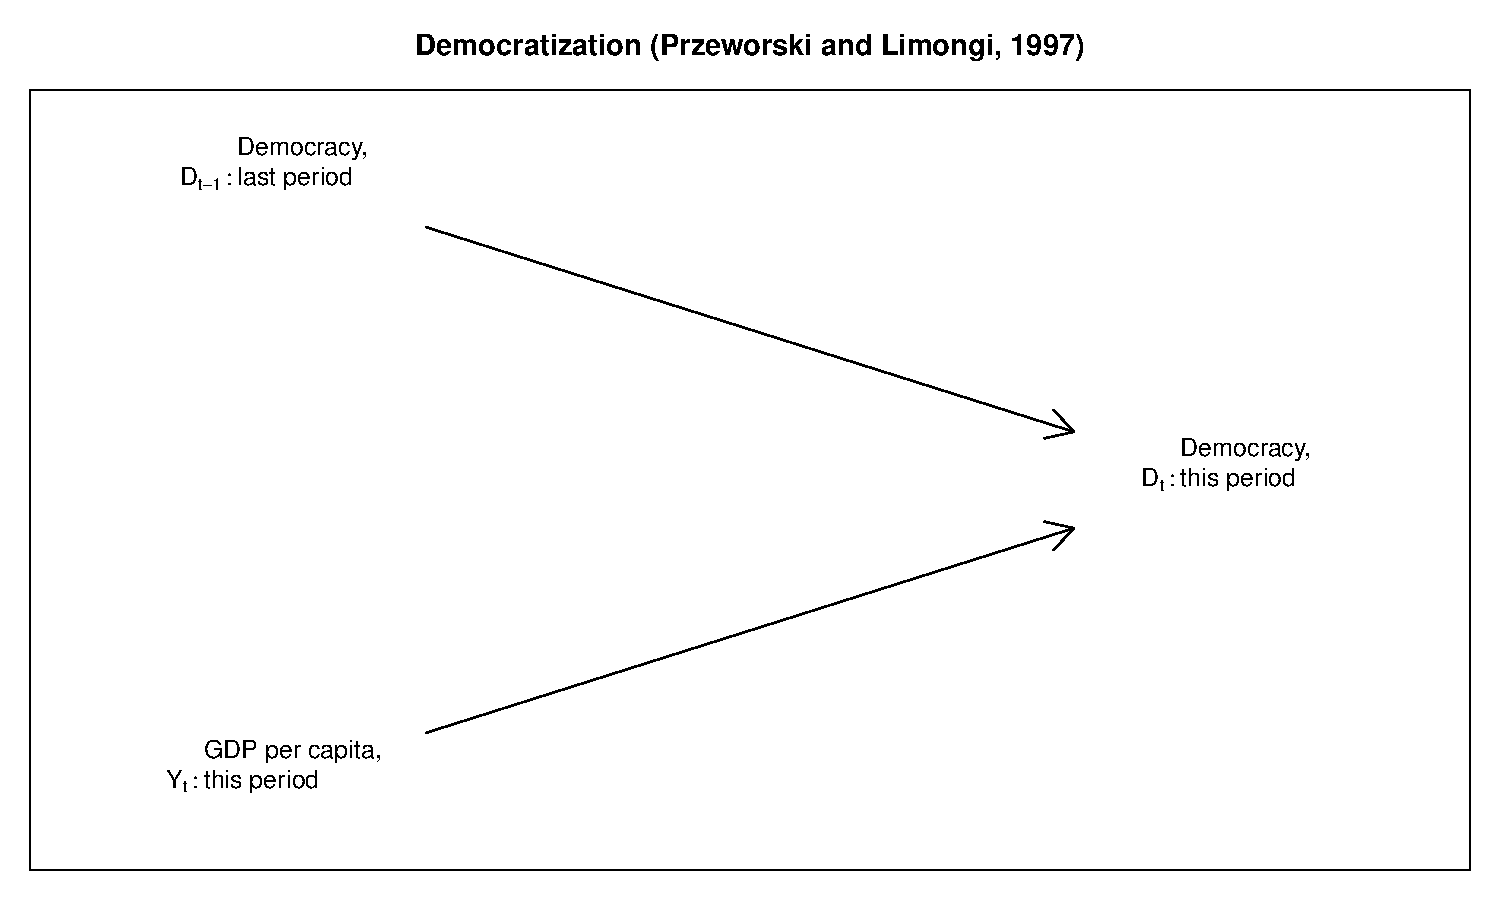
\includegraphics[width=.7\textwidth]{ii_files/figure-latex/DAGPL-1} 

}

\caption{A graphical representation of Przeworski and Limongi's argument, where $D_{t-1}$=democracy in the previous period; $GDP_t$=per capita GDP in the current period; $D_t$=democracy in the current period.}\label{fig:DAGPL}
\end{figure}

Second, the arrow running from \(GDP_{t-1}\) to \(D_t\) means that \(GDP\) \emph{may} affect democracy, not that it always does. Indeed, Przeworski and Limongi's argument is that development's effect depends on a regime's prior state: GDP matters for whether democracies continue to be democracies, but not for whether autocracies go on to become democracies. The absence of an arrow between \(D_{t-1}\) and \(GDP_{t-1}\), however, implies a (possibly incorrect) belief that democracy and \(GDP\) in the last period are independent of one another.

Inspection of this figure highlights, we think, a curious feature of this argument. The key claim---that the switch \emph{to} democracy does not depend on income---is not readable from the graph. The reason is simply that, given this argument, being a non democracy in one period given you were a democracy in a previous period does depend on income. Your state in the second period does depend on income. Specifically there is a \emph{counterfactual} dependence---income causes a state to be democratic even if it does not cause it to \emph{transition to} democracy. The effect of income may well be asymmetric depending on whether you start as a democracy or start as an autocracy but this asymmetry has to be be captured by the specification of the functional relations; it is not captured by the graph.

For a parametric representation of this asymmetric relationship we can specify a function in which \(GDP\) can reduce the likelihood of a transition \emph{away} from democracy but does affect the probability of a transition \emph{to} democracy, which should be exogenously determined. One possible translation of the argument into functional terms is:

\[D_t = \mathbb{1}(\theta^{D_t} + (1-D_{t-1})p + D_{t-1}Y_{t-1}q) > 0)\]

where

\begin{itemize}
\tightlist
\item
  \(D_t\) and \(D_{t-1}\) are binary, representing current and last-period democracy, respectively
\item
  \(p\) is a parameter representing the probability that an autocracy democratizes
\item
  \(q\) is a parameter representing the probability that a democracy with a GDP of 1 remains democratic
\item
  \(Y_{t-1}\) represents national per capita GDP, scaled to 0-1.
\item
  \(\theta^{D_t}\) represents a random, additional input into democracy
\item
  the indicator function, \({1}\), evaluates the inequality and generates a value of \(1\) if and only if it is true
\end{itemize}

Unpacking the equation, the likelihood that a country is a democracy in a given period rises and falls with the expression to the left of the inequality operator. This expression itself has two parts, reflecting the difference between the determinants of \emph{transitions to} democracy (captured by the first part) and the determinants of democratic \emph{survival} (captured by the second). The first part comes into play---i.e., is non-zero---only for non-democracies. For non-democracies, the expression evaluates simply to \(p\), the exogenous probability of democratization. The second part is non-zero only for democracies, where it evaluates to \(q\) times \(Y_{t-1}\): thus, remaining democratic is more likely as national income rises. The inequality is then evaluated by asking whether the expression on the left passes a threshold. Thus, higher values for the expression increase the likelihood of democracy while the randomness of the \(\theta^{D_t}\) threshold captures the role of other, idiosyncratic inputs. The mean and variance of \(\theta^{D_t}\) capture the overall likelihood of being a democracy as well as the importance of unspecified factors.\footnote{Note how, while the functional equation nails down certain features of the process, it leaves others up for grabs. In particular, the parameters \(p\) and \(q\) are assumed to be constant for all autocracies and for all democracies, respectively, but their values are left unspecified. And one could readily write down a function that left even more openness---by, for instance, including an unknown parameter that translates \(y\) into a change in the probability of reversion or allowing for non-linearities, with unknown parameters, in this effect.} In a model like this it would be natural to seek to estimate parameters \(p\) and \(q\) as well as trying to understand the distribution of \(\theta^{D_t}\).

We can also represent the asymmetry in the binary set up with causal types that we developed in the last chapter.

Type \(\theta^{D_t}_{0001}\) is a type for which the regime type \emph{will stay as they are} if they are wealthy, but will become authoritarian if they are not wealthy. To be clear, wealth still affects whether or not a state is a democracy, rather than an autocracy, in this period--counterfactually---but wealth does not make a non democracy become a democracy. In other words it causes a case to \emph{be} a democracy but not to \emph{become} a democracy. This type can be distinguished from a \(\theta^{D_t}_{0011}\) type in which a non democracy becomes a democracy when income is high.

Although we do not engage with dynamic models in this book, it is instructive to think through the implications of a distribution of causal types for a dynamic process. Say we were to imagine that income were constant but that in each period one half of units were of type \(\theta^{D_t}_{0001}\), and one half of type \(\theta^{D_t}_{1111}\) (with types drawn afresh each period). Say that in an initial period, half the units were democracies and half had high income and there was no relation between these two features. Then in the next period we would have that
half of cases would be democracies (regardless of income), half of which would be surviving democracies and half new democracies; of the other half, one quarter would be surviving democracies (surviving \emph{because of} their income), and the other three quarters would be autocracies, one third of which would be ``backsliders'' because of their poverty. Similar transitions occur in future periods until eventually the wealthy states are all stable democracies and the poorer states transition between democracy and autocracy back and forth randomly each period.

In this approach there are no parameters \(p\) or \(q\) to be estimated. Rather the focus is entirely on the distribution of nodal types.

\hypertarget{questions}{%
\chapter{Causal Queries}\label{questions}}

\begin{headerbox}
We describe major families of causal queries and illustrate how these can all be described as queries about the values of nodes in a causal model.

\end{headerbox}

Although scholars share a broad common interest in causality there is tremendous heterogeneity in the kinds of causal questions that scholars ask. Consider the relationship between inequality and democratization. We might seek, for instance, to know inequality's average impact on democratization across some set of cases. Alternatively, we might be interested in a particular case---say, Mongolia in 1995---and want to know whether inequality would have an effect \emph{here}. That is a question about causal effects at the case level. Alternatively we might wonder whether the level of democracy in Mongolia in 1995 is \emph{due} to the level of inequality in that case---this is quite a distinct question (in the same way that establishing that poison would make you sick does not imply that you are sick because of poison). Or we may be interested in \emph{how} causal effects unfold, inquiring about the pathway or mechanism through which inequality affects democratization---a question we can also ask at two levels. We can ask whether inequality affected democratization in Mongolia through mobilization of the masses; or we can ask how commonly inequality affects democratization through mobilization across a broad set of cases. Pushing further we might ask a counterfactual question of the form: would inequality have produced democratization had mobilization been prevented from occurring.

Distinct methodological literatures have been devoted to the study of average causal effects, the analysis of case-level causal effects and explanations, and the identification of causal pathways. Fortunately each of these questions can be readily captured as specific queries asked of (and answerable from) a causal model. As described by \citet{judea2010introduction}, the goal is to deploy an ``\emph{algorithm} that receives a model \emph{M} as an input and delivers the desired quantity \emph{Q(M)} as the output.'' More specifically, we demonstrate how, given the structure we described in Chapter \ref{models}, causal queries can be represented as question about one or more \emph{nodes} on a causal graph. When we assimilate our causal questions into a causal model, we are placing what we want to know in formal relation to both what we \emph{already} know and what we can potentially \emph{observe}. As we will see in later chapters, this move allows us then to deploy the model to generate strategies of inference: to determine which observations, if we made them, would be likely to yield the greatest leverage on our query, given our prior knowledge about the way the world works. And by the same logic, once we see the evidence, this integration allows us to ``update'' on our query---figure out in systematic fashion what we \emph{have} learned---in a manner that takes background knowledge into account.

In the remainder of this chapter, we walk through the conceptualization and causal-model interpretation of five key causal queries:

\begin{itemize}
\item
  Case-level causal effects
\item
  Case-level causal attribution
\item
  Case-level explanation
\item
  Average causal effects
\item
  Causal pathways
\end{itemize}

These five are in no way exhaustive of the causal questions that can be captured in causal graphs, but they are among the more common social scientific investigations.

\hypertarget{case-level-causal-effects}{%
\section{Case-level causal effects}\label{case-level-causal-effects}}

The simplest causal question is whether some causal effect operates in an individual case. Does \(X\) have an effect on \(Y\) in this case? For instance, is Yemen in 1995 a case in which a change in economic inequality would produce a change in whether or not the country democratizes? We could put the question more specifically as a query about a causal effect in a particular direction, for instance: Does inequality have a positive effect on democratization in the case of Yemen in 1995?

In counterfactual terms, a query about case-level causation is a question about what would happen if we could manipulate a variable in the case: if we could hypothetically intervene to change \(X\)'s value in the case, (how) would \(Y\)'s value change? To ask whether a positive (or negative) effect operates for a case is to ask whether a particular counterfactual relation holds in that case. If we assume a setup with binary variables for simplicity, to ask whether inequality has a positive effect on democratization is to ask: if we set \(I\) to \(0\) would \(D\) take on a value of \(0\), \emph{and} if we set \(I\) to \(1\), would \(D\) take on a value of \(1\)? (\emph{Both} of these conditions must hold for \(I\) to have a positive effect on \(D\).)

We can easily represent this kind of query in the context of a causal model. We show the DAG for such a model in Figure \ref{fig:casequery}. As introduced in Chapter \ref{models}, \(\theta^Y\) here represents the nodal type characterizing \(Y\)'s response to \(X\) and, if \(X\) and \(Y\) are binary, it can take on one of four values: \(\theta^Y_{10}\), \(\theta^Y_{01}\), \(\theta^Y_{00}\), and \(\theta^Y_{11}\) (which map onto our \(a, b, c\) and \(d\) types, respectively). Importantly, given that the value of nodes (or variables) is allowed to vary across cases, this setup allows for \(\theta^Y\)---the causal effect of \(X\) on \(Y\)---to vary across cases. Thus, \(X\) may have a positive effect on \(Y\) in one case (with \(\theta^Y=\theta^Y_{01}\)), and a negative (\(\theta^Y=\theta^Y_{10}\)) or no effect (\(\theta^Y=\theta^Y_{00}\) or \(\theta^Y_{11}\)) on \(Y\) in other cases.

\begin{figure}

{\centering 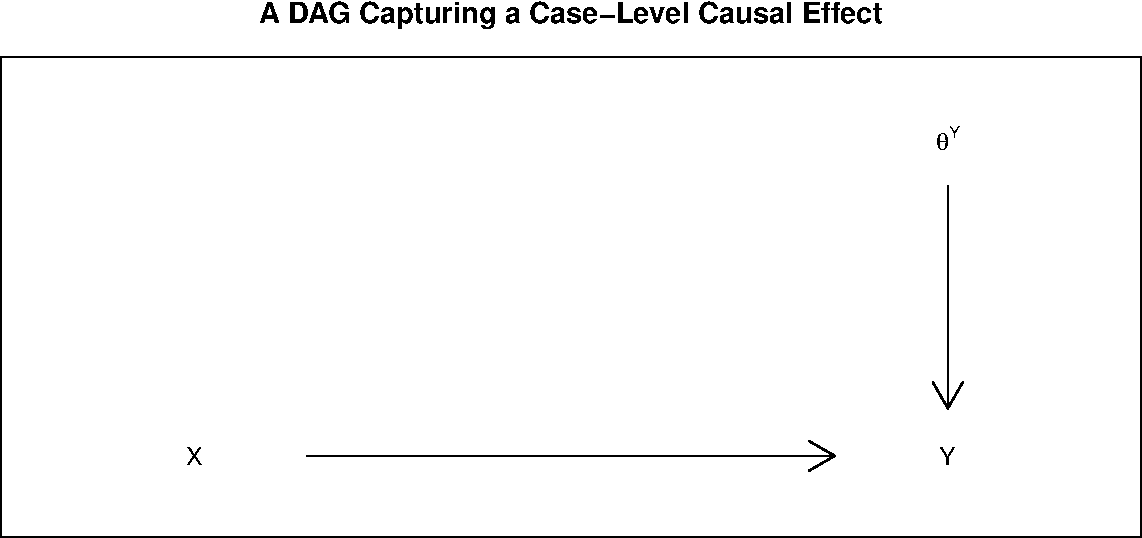
\includegraphics[width=0.6\linewidth]{ii_files/figure-latex/casequery-1} 

}

\caption{This DAG is a graphical representation of the simple causal setup in which the effect of $X$ on $Y$ in a given case depends on the case's nodal type, represented by $\theta^Y$. With a single binary causal variable of interest, we let $\theta^Y$ take on values $\theta^Y_{ij}$, with $i$ representing the value $Y$ takes on if $X=0$ and $j$ representing the value $Y$ takes on if $X=1$. With a binary framework outcome, $\theta^Y$ ranges over the four values: $\theta^Y_{00}$, $\theta^Y_{10}$, $\theta^Y_{01}$ and $\theta^Y_{11}$.}\label{fig:casequery}
\end{figure}

In this model, then, the query, ``What is \(X\)'s causal effect in this case?'' simply becomes \emph{a question about the value of the nodal type \(\theta^Y\)}.

Two natural variants of this question are, ``What is the expected effect of \(X\) on \(Y\)?'' and "What is the probability that \(X\) matters for \(Y\)? Answering the question requires estimating the probability that \(X\) has a positive effect minus the probability that it has a negative effect: \(\Pr(\theta^Y = \theta^Y_{01}) - \Pr(\theta^Y = \theta^Y_{10})\). Answering the second involves assessing \(\Pr(\theta^Y = \theta^Y_{01} \text{ OR } \theta^Y = \theta^Y_{10})\).

We can conceptualize this same question even if the model involves more complex relations between \(X\) and \(Y\). The question itself does not depend on the model having a particular form. For instance, consider a mediation model of the form \(X\rightarrow M \rightarrow Y\). In this model, a positive effect of \(X\) on \(Y\) can emerge either from a chain of positive effects of \(X\) on \(M\) and of \(M\) on \(Y\) or from a chain of negative effects, while a negative effect of \(X\) on \(Y\) can emerge from a chain of opposite-signed effects. Thus, answering the question means estimating:

\begin{equation}
\begin{split}
\Pr((\theta^M = \theta^M_{01} \& \theta^Y = \theta^Y_{01})  \text{ OR }  (\theta^M = \theta^M_{10} \& \theta^Y = \theta^Y_{10}))   - \\
\Pr((\theta^M = \theta^M_{01} \& \theta^Y = \theta^Y_{10})  \text{ OR }  (\theta^M = \theta^M_{10} \& \theta^Y = \theta^Y_{01}))
\end{split}
\end{equation}

\emph{Answering} the question now requires guesses about nodal types for \(M\) and for \(Y\), not just nodal types for \(Y\). Thus the question remains the same, and answerable, under different models, but the answer to the question might involve summaries of the values of different nodes.

\hypertarget{case-level-causal-attribution}{%
\section{Case-level causal attribution}\label{case-level-causal-attribution}}

A query about causal attribution is related to, but different from, a query about a case-level causal effect. When asking about \(X\)'s case-level effect, we are asking, ``\emph{Would} a change in \(X\) cause a change in \(Y\) in this case?'' The question of causal attribution asks: ``\emph{Did} \(X\) cause \(Y\) to take on the value it did in this case?'' More precisely, we are asking, ``Given the values that \(X\) and \(Y\) \emph{in fact} took on in this case, would \(Y\)'s value have been different if \(X\)'s value had been different?''

For instance, given that we know that inequality in Taiwan was relatively low and that Taiwan democratized in 1996, was low inequality a \emph{cause} of Taiwan's democratization in 1996? Or: given low economic inequality and democratization in Taiwan in 1996, would the outcome in this case have been different if inequality had been high?

This goes beyond simply asking whether Taiwan is a case in which inequality has a causal effect on democratization. Whereas a case-level causal effect is defined in terms of the \(\theta\) nodes on endogenous variables, we define a causal-attribution query in terms of a larger set of nodes. To attribute \(Y\)'s value in a case to \(X\), we need to know not only whether this is the kind of case in which \(X\) could have an effect on \(Y\) but also whether the context is such that \(X\)'s value \emph{in fact} made a difference.

Consider, for instance, the general setup in Figure \ref{fig:attribquery}. Here, \(Y\) is a function of two variables, \(X_1\) and \(X_2\). This means that \(\theta^Y\) is somewhat more complicated than in a setup with one causal variable: \(\theta^Y\) must here define \(Y\)'s response to all possible combinations of \(X_1\) and \(X_2\), including interactions between them.

\begin{figure}

{\centering 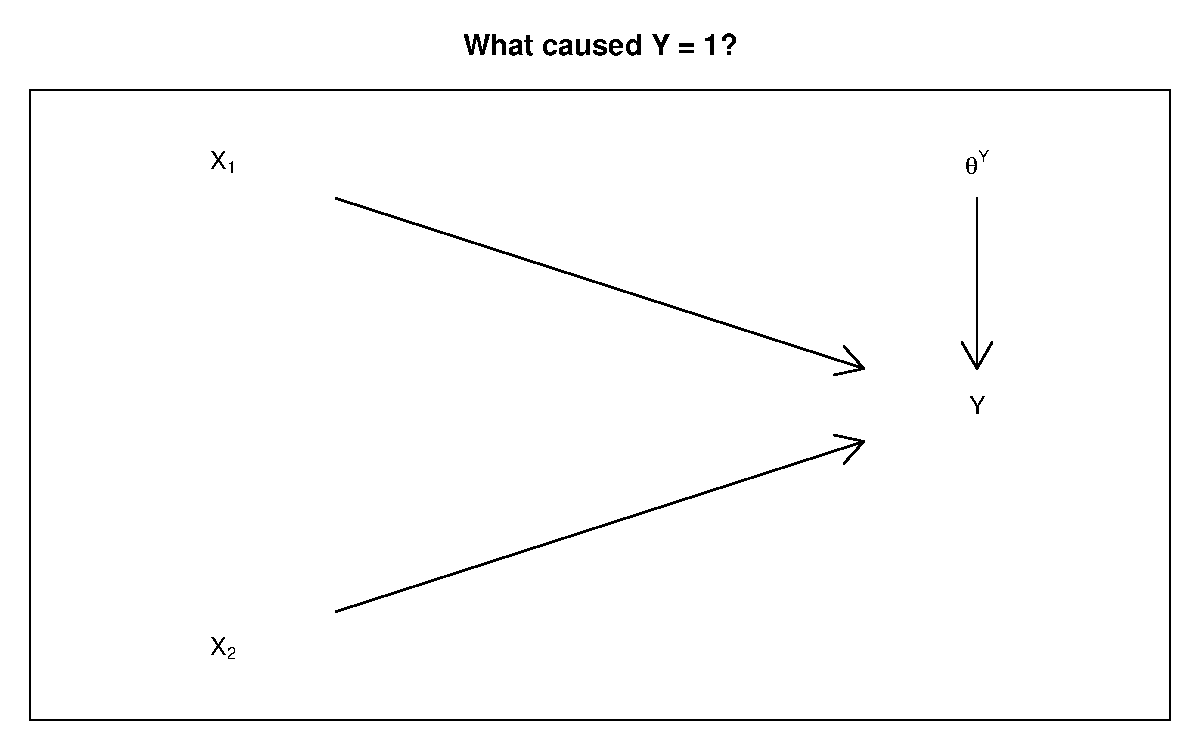
\includegraphics[width=0.6\linewidth]{ii_files/figure-latex/attribquery-1} 

}

\caption{This DAG is a graphical representation of the simple causal setup in which $Y$ depends on two variables $X1$ and $X2$. How $Y$ responds to X1 and X2 depnds on $\theta^Y$, the DAG itself does not provide information on whether or how X1 and X2 interact with each other.}\label{fig:attribquery}
\end{figure}

We examined the set of nodal types for a set up like this in Chapter 2 (see Table \ref{tab:PO16}). In the table, there are four column headings representing the four possible combinations of \(X_1\) and \(X_2\) values. Each row represents one possible pattern of \(Y\) values as \(X1\) and \(X2\) move through their four combinations.

One way to conceptualize the size of the nodal-type ``space'' is to note that \(X_1\) can have any of our four causal effects (the four binary types) on \(Y\) when \(X_2=0\); and \(X_1\) can have any of four causal effects when \(X_2=1\).\footnote{This is precisely equivalent to noting that \(X_2\)'s effect on \(Y\) can be of any of the four types when \(X_1=0\) and of any of the four types when \(X_1=1\).} This yields 16 possible response patterns to combinations of \(X_1\) and \(X_2\) values.

A query about causal attribution---whether \(X_1 = 1\) caused \(Y=1\)---for the model in Figure \ref{fig:attribquery}, needs to be defined in terms of both \(X_2\) and \(\theta^Y\). Parallel to our Taiwan example, suppose that we have a case in which \(Y=1\) and in which \(X_1\) was also 1, and we want to know whether \(X_1\) caused \(Y\) to take on the value it did. Answering this question requires knowing whether the case's type is such that \(X_1\) would have had a positive causal effect on \(Y\), \emph{given the value of \(X_2\)} (which we can think of as part of the context). Thus, given that we start with knowledge of \(X_1\)'s and \(Y\)'s values, our query about causal attribution amounts to a query about two nodal types: (a) \(\theta^{X_2}\) (which gives \(X_2\)'s value) and (b) \(\theta^Y\), specifically whether its value is such that \(X_1\) has a positive causal effect given \(X_2\)'s value.

Suppose, for instance, that we were to observe \(X_2=1\). We then need to ask whether the nodal type, \(\theta^Y\), is such that \(X_1\) has a positive effect when \(X_2=1\). Consider \(\theta^Y_{0111}\) (type 8 in Table \ref{tab:PO16}).\footnote{A reminder that, with two-parent nodes, the nodal-type subscript ordering is \(Y|(X_1=0, X_2=0); Y|(X_1=1, X_2=0); Y|(X_1=0, X_2=1); Y|(X_1=1, X_2=1)\).} This is a nodal type in which \(X_1\) has a positive effect when \(X_2=0\) but no effect when \(X_2=1\). Put differently, \(X_2=1\) is a sufficient condition for \(Y=1\), meaning that \(X_1\) makes no difference to the outcome when \(X_2=1\).

In all we have four qualifying \(Y\)-types: \(\theta^Y_{0001}\), \(\theta^Y_{1001}\), \(\theta^Y_{0101}\), \(\theta^Y_{1101}\). In other words, we can attribute a \(Y=1\) outcome to \(X_1=1\) when \(X_2=1\) and \(Y\)'s nodal type is one of these four.

Thus, a question about causal attribution is a question about the \emph{joint} value of a set of nodal types: about whether the \emph{combination} of context and the nodal type(s) governing effects is such that changing the causal factor of interest would have changed the outcome.

\hypertarget{actual-causes}{%
\section{Actual causes}\label{actual-causes}}

So far we have been dealing with causes in the standard counterfactual sense: a change in antecedent conditions which would have produced a different outcome. Sometimes, however, we are interested in identifying antecedent conditions that were not counterfactual difference-makers but that nonetheless \emph{generated} or \emph{produced} the outcome. Consider, for instance, a situation in which an outcome was overdetermined: multiple conditions were present, each of which on their own, \emph{could} have generated the outcome. Then none of these conditions caused the outcome in the counterfactual sense; yet one or more of them may have been distinctively important in \emph{producing} the outcome. The concept of an \emph{actual cause} can be useful in putting a finer point on this kind of causal question.

A motivating example used in much of the literature on actual causes \citep[e.g.][]{hall2004two} imagines two characters, Sally and Billy, simultaneously throwing stones at a bottle. Both are excellent shots and hit whatever they aim at. Sally's stone hits first, and so the bottle breaks. However, Billy's stone \emph{would} have hit had Sally's not hit, and would have broken the bottle. Did Sally's throw cause the bottle to break? Did Billy's?

By the usual definition of causal effects, neither Sally's nor Billy's action had a causal effect: without either throw, the bottle would still have broken. We commonly encounter similar situations in the social world. We observe, for instance, the onset of an economic crisis and the breakout of war---either of which would be sufficient to cause the government's downfall---but with (say) the economic crisis occurring first and toppling the government before the war could do so. In this situation, neither economic crisis nor war in fact made a difference to the outcome: take away either one and the outcome remains the same.

To return to the bottle example, while neither Sally's nor Billy's throw is a counterfactual cause, there is an important sense in which Sally's action obviously broke the bottle, and Billy's did not. We can formalize this intuition by defining Sally's throw as the \emph{actual cause} of the outcome. Using the definition provided by \citep{halpern2015modification}, building on \citep{halpern2005causesa} and others, we say that a condition (\(X\) taking on some value \(x\)) was an actual cause of an outcome (of \(Y\) taking on some value \(y\)), where \(x\) and \(y\) may be collections of events, if:

\begin{enumerate}
\def\labelenumi{\arabic{enumi}.}
\tightlist
\item
  \(X=x\) and \(Y=y\) both happened
\item
  there is some set of variables, \(\mathcal W\), such that if they were fixed at the levels that they actually took in the case, and if \(X\) were to be changed, then \(Y\) would change (where \(\mathcal W\) can also be an empty set)
\item
  no strict subset of \(X\) satisfies 1 and 2 (there is no redundant part of the condition, \(X=x\))
\end{enumerate}

The definition thus describes a condition that \emph{would} have been a counterfactual cause of the outcome if we were to imagine holding constant some set of events that in fact occurred (and that, in reality, might not have been constant if the actual cause had not in fact occurred).

Let us now apply these 3 conditions to the Sally and Billy example. Conditions 1 and 3 are easily satisfied, since Sally \emph{did} throw and the bottle \emph{did} break (Condition 1), and ``Sally threw'' has no strict subsets (Condition 3).

Condition 2 is met if Sally's throw made a difference, counterfactually speaking --- with the important caveat that, in determining this, we are permitted to condition on (to fix in the counterfactual comparison) any event or set of events that actually happened (or on on none at all). To see why Condition 2 is satisfied, we have to think of there being three steps in the process: (1) Sally and Billy throw, (2) Sally's or Billy's rock hits the bottle, and (3) the bottle breaks. In actuality, Billy's stone did not hit the bottle, so we are allowed to condition on that fact in determining whether Sally's throw was a counterfactual cause. Conditioning on Billy's stone not hitting, the bottle would \emph{not} have broken had Sally not thrown.

From the perspective of counterfactual causation, it may seem odd to condition on Billy's stone not hitting the bottle when thinking about Sally not throwing the stone---since Sally's throwing the stone was the very thing that prevented Billy from hitting the bottle. Yet Halpern argues that this is an acceptable thought experiment for establishing the importance of Sally's throw since conditioning is constrained to the actual facts of the case. Moreover, the same logic shows why Billy is not an actual cause. The reason is that Billy's throw is only a cause in those conditions in which Sally did not hit the bottle. But because Sally \emph{did} actually hit the bottle, we are not permitted to condition on Sally not hitting the bottle in determining actual causation. We thus cannot---even through conditioning on actually occurring events---construct any counterfactual comparison in which Billy's throw is a counterfactual cause of the bottle's breaking.

The striking result here is that there can be grounds to claim that a condition was the actual cause of an outcome even though, under the counterfactual definition, the effect of that condition on the outcome is 0. (At the same time, all counterfactual causes are automatically actual causes; they meet Condition 2 by conditioning on nothing at all, an empty set \(\mathcal W\).) One immediate methodological implication follows: since actual causes need not be causes, there are risks in research designs that seek to understand causal effects by tracing back actual causes---i.e., the way things actually happened. If we traced back from the breaking of the bottle, we might be tempted to identify Sally's throw as the cause of the outcome. We would be right only in an actual-causal sense, but wrong in the standard, counterfactual causal sense. Chains of events that appear to ``generate'' an outcome are not always causes in that sense.\footnote{Perhaps more surprising, it is possible that the expected causal effect is negative but that \(X\) is an actual cause in expectation. For instance, suppose that 10\% of the time Sally's shot intercepts Billy's shot but without hitting the bottle. In that case the average causal effect of Sally's throw on bottle breaking is \(-0.1\) yet 90\% of the time Sally's throw is an actual cause of bottle breaking (and 10\% of the time it is an actual cause of non-breaking). For related discussions, see \citet{menzies1989probabilistic}.}

As with other causal queries, the question ``Was \(X=x\) the actual cause of \(Y=y\)?'' can be redefined as a question about which combinations of nodal types produce conditions under which \(X\) could have made a difference. To see how, let us run through the Billy and Sally example again, but formally in terms of a model. Consider Figure \ref{fig:actualquery}, where we represent Sally's throw (\(S\)), Billy's throw (\(B\)), Sally's rock hitting the bottle (\(H^S\)), Billy's rock hitting the bottle (\(H^B\)), and the bottle cracking (\(C\)). Each endogenous variable has a \(\theta\) term associated with it, capturing its nodal type. We capture the possible ``preemption'' effect with the arrow pointing from \(H^S\) to \(H^B\), allowing whether Sally's rock hits to affect whether Billy's rock hits.\footnote{We do not need an arrow in the other direction because Sally throws first.}

For Sally's throw to be an actual cause of the bottle's cracking, we need first to establish that Sally threw (\(\theta^S=\theta^S_1\)) and that the bottle cracked (\(\theta^C=\theta^C_1\)) (Condition 1). Condition 3 is automatically satisfied in that \(\theta^S=\theta^S_1\) has no strict subsets. Turning now to Condition 2, we need Sally's throw to be a counterfactual cause of the bottle cracking if we condition on the value of some set of nodes remaining fixed at the values they in fact took on. As discussed above, we know that we can meet this criterion if we condition on Billy's throw not hitting. To make this work, we need to ensure, first, that Sally's throw hits if and only if she throws: so \(\theta^{H^S}=\theta^{H^S}_{01}\). Next, we need to ensure that Billy's throw does not hit whenever Sally's does: this corresponds to any of the four nodal types for \(H^B\) that take the form \(\theta^{H^B}_{xx00}\), meaning that \(H^B=0\) whenever \(H^S=1\). Note that the effect of Billy throwing on Billy hitting when Sally has \emph{not} thrown---the first two terms in the nodal-type's subscript---does not matter since we have already selected a value for \(\theta^S\) such that Sally does indeed throw.

Finally, we need \(\theta^C\) to take on a value such that \(H^S\) has a positive effect on \(C\) when \(H^B=0\) (Billy doesn't hit) since this is the actual circumstance on which we will be conditioning. This is satisfied by any of the four nodal types of the form \(\theta^C_{0x1x}\). This includes, for instance, a \(\theta^C\) value in which Billy's hitting has no effect on the bottle (perhaps Billy doesn't throw hard enough!): e.g., \(\theta^C_{0011}\). Here, Sally's throw is a counterfactual cause of the bottle's cracking. And, as we have said, all counterfactual causes are actual causes. They are, simply, counterfactual causes when we hold \emph{nothing} fixed (\(\mathcal W\) in Condition 2 is just the empty set).

Notably, we do not need to specify the nodal type for \(B\): given the other nodal types identified, Sally's throw will be the actual cause regardless of whether or not Billy throws. If Billy does not throw, then Sally's throw is a simple counterfactual cause (given the other nodal types).

The larger point is that actual cause queries can, like all other causal queries, be defined as questions about the values of nodes in a causal model. When we pose the query, was Sally's throw an actual cause of the bottle cracking, we are in effect asking whether the case's combination of nodal types (or its causal type) matches \(\theta^S_1, \theta^B_x, \theta^{H^B}_{xx00}, \theta^{H^S}_{01}, \theta^C_{0x1x}\).

Likewise, if want to ask \emph{how often} Sally's throw is an actual cause, in a population of throwing rounds, we can address this query as a question about the joint \emph{distribution} of nodal types. We are then asking how common the qualifying combinations of nodal types are in the population given the distribution of types at each node.

\begin{figure}

{\centering 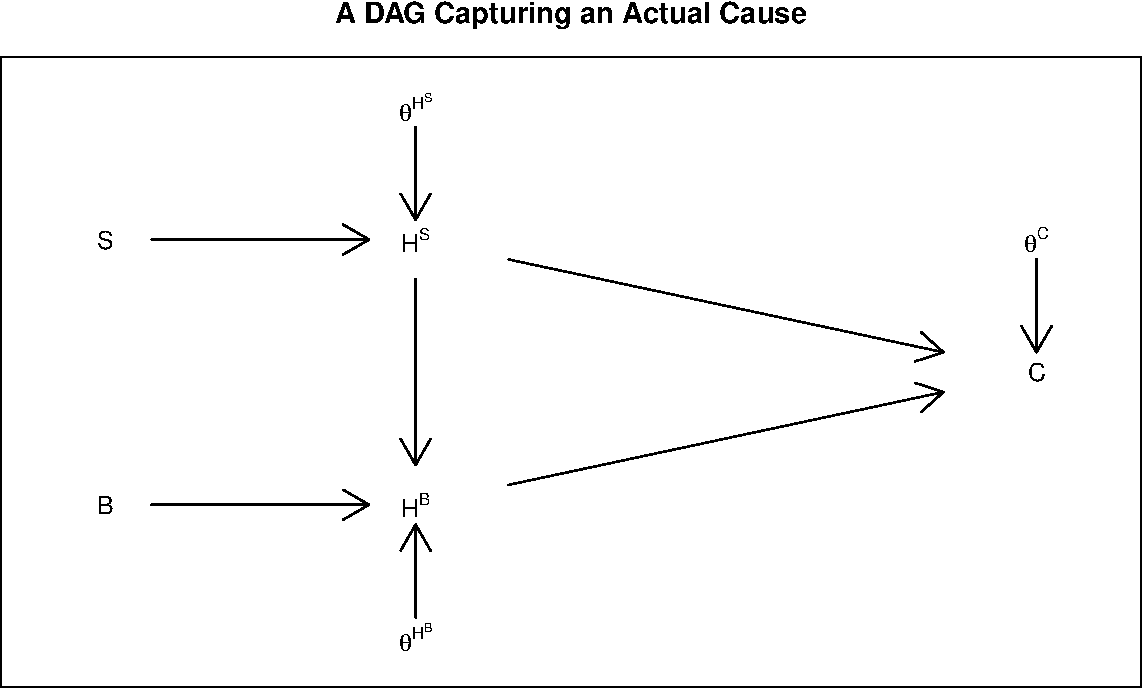
\includegraphics[width=0.6\linewidth]{ii_files/figure-latex/actualquery-1} 

}

\caption{This DAG is a graphical representation of the simple causal setup in which the effect of $X$ on $Y$ in a given case depends on the case's nodal type for $Y$, represented by $\theta^Y$.}\label{fig:actualquery}
\end{figure}

Actual causes are conceptually useful whenever there are two sufficient causes for an outcome, but one preempts the operation of the other. For instance, we might posit that both the United States' development of the atomic bomb was a sufficient condition for U.S. victory over Japan in World War II, and that U.S. conventional military superiority was also a sufficient condition and would have operated via a land invasion of Japan. Neither condition was a counterfactual cause of the outcome because both were present. However, holding constant the \emph{absence} of a land invasion, the atomic bomb was a difference-maker, rendering it an actual cause. The concept of actual cause thus helps capture the sense in which the atomic bomb distinctively contributed to the outcome, even if it was not a counterfactual cause.

An extended notion \citep[p 81]{halpern2016actual} of actual causes restricts the imagined counterfactual deviations to states that are more likely to arise (more ``normal'') than the factual state. We will call this notion a ``notable cause.'' We can say that one cause, \(A\), is ``more notable'' than another cause, \(B\), if a deviation in \(A\) from its realized state is (believed to be) more likely than a deviation in \(B\) from its realized state.

For intuition, we might wonder why a Republican was elected to the presidency in a given election. In looking at some minimal winning coalition of states that voted Republican, we might distinguish between a set of states that \emph{always} vote Republican and a set of states that usually go Democratic but voted Republican this time. If the coalition is minimal winning, then every state that voted Republican is a cause of the outcome in the standard (difference-making) sense. However, only the states that usually vote Democratic are notable causes since it is only for them that the counterfactual scenario (voting Democratic) was more likely to arise than the factual scenario. In a sense, we take the ``red'' states' votes for the Republican as given---placing them, as it were, in the causal background---and identify as ``notable'' those conditions that mattered and easily could have gone differently. By the same token, we can say that, among those states that voted Republican this time, those that more commonly vote Democratic are \emph{more} notable causes than those that less commonly vote Democratic.

How notable a counterfactual cause is can be expressed as a claim about the distribution of a set of nodal types. For instance, if we observe \(R^j=1\) for state \(j\) (it voted Republican), then the notability of this vote directly increases in our belief about the probability that \(\theta^{R^j}=\theta_0^{R^j}\): the probability that the state's vote could have gone the other way.

\hypertarget{average-causal-effects}{%
\section{Average causal effects}\label{average-causal-effects}}

A more general query asks about an average causal effect in some population. In counterfactual terms, a question about average causal effects is: if we manipulated the value of \(X\) for all cases in the population---first setting \(X\) to one value for all cases, then changing it to another value for all cases---by how much would the average value of \(Y\) in the population change? Like other causal queries, a query about an average causal effect can be conceptualized as learning about a node in a causal model.

We can do this by conceiving of any given case as being a member of a population composed of different nodal types. When we seek to estimate an average causal effect, we seek information about the \emph{shares} of these nodal types in the population.

More formally and adapted from \citet{humphreys2015mixing}, we can use \(\lambda^Y_{ij}\) to refer to the \emph{share} of cases in a population that has nodal type \(\theta^Y_{ij}\). Thus, given our four nodal types in a two-variable binary setup, \(\lambda^Y_{10}\) is the proportion of cases in the population with negative effects; \(\lambda_{01}\) is the proportion of cases with positive effects; and so on. One nice feature of this setup, with both \(X\) and \(Y\) as binary, is that the average causal effect can be simply calculated as the share of positive-effect cases less the share of negative-effect cases: \(\lambda^Y_{01} - \lambda^Y_{10}\).

Graphically, we can represent this setup by including \(\lambda^Y\) in a more complex causal graph as in Figure \ref{fig:DAGace}. As in our setup for case-level causal effects, \(X\)'s effect on \(Y\) in a case depends on (and only on) the case's nodal type, \(\theta^Y\). The key difference is that we now model the case's type not as exogenously given, but as a function of two additional variables: the distribution of nodal types in a population and a random process through which the case's type is ``drawn'' from that distribution. We represent the type distribution as \(\lambda^Y\) (a vector of values for the proportions \(\lambda^Y_{10}, \lambda^Y_{01}, \lambda^Y_{00}, \lambda^Y_{11}\)) and the random process drawing a \(\theta^Y\) value from that distribution as \(U^\theta\).

In this model, our causal query---about \(X\)'s average causal effect---is thus defined by the vector \(\lambda^Y\), and specifically by the shares of negative- and positive-causal-effect cases, respectively, in the population. What is \(X\)'s average effect on \(Y\) amounts to asking: what are the values of \(\lambda^Y_{10}\) and \(\lambda^Y_{01}\)? As with \(\theta^Y\), \(\lambda^Y\) is not directly observable. And so the empirical challenge is to figure out what we \emph{can} observe that would allow us to learn about \(\lambda^Y\)'s component values?\footnote{Note also that \(\lambda^Y\) can be thought of as itself drawn from a distribution, such as a Dirichlet. The hyperparameters of this underlying distribution of \(\lambda\) would then represent our uncertainty over \(\lambda\) and hence over average causal effects in the population.}

\begin{figure}

{\centering 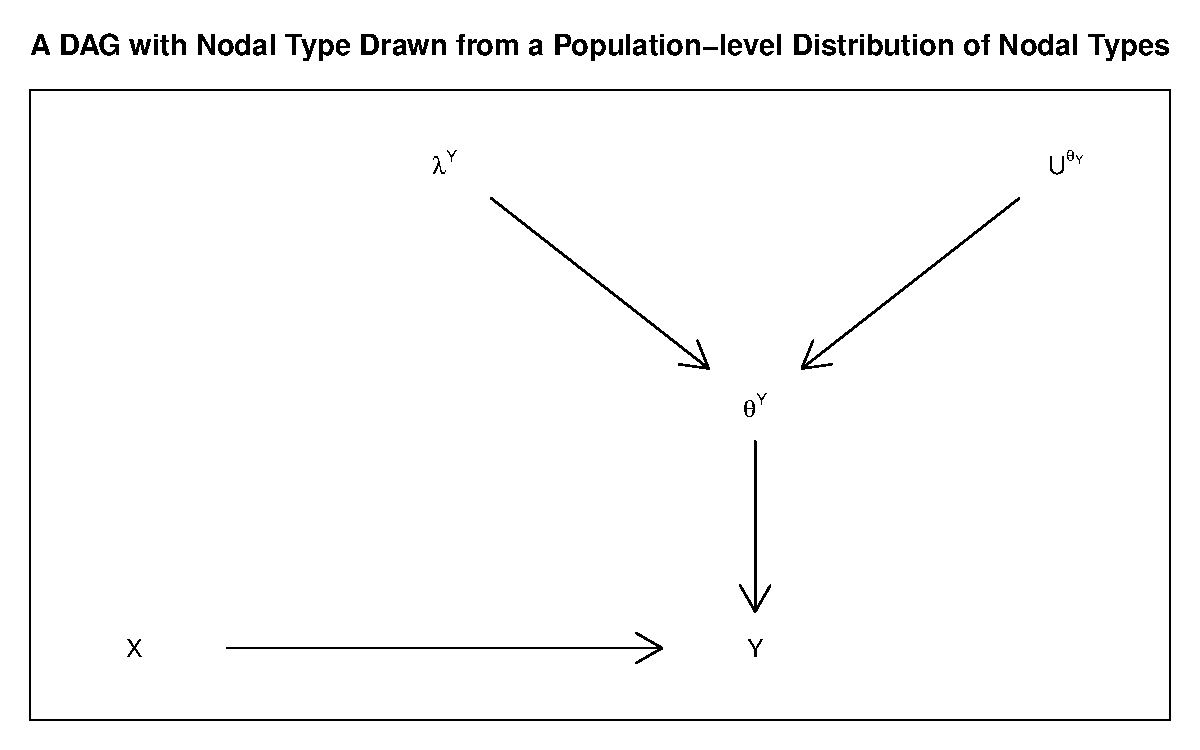
\includegraphics[width=0.6\linewidth]{ii_files/figure-latex/DAGace-1} 

}

\caption{This DAG is a graphical representation of a causal setup in which cases are drawn from a population composed of different nodal types. As before, $X$'s effect on $Y$ is a function of a causal-type variable, $\theta^Y$. Yet here we explicitly model the process through which the case's type is drawn from a distribution of types in a population. The variable $\lambda$ is a vector representing the multinomial distribution of nodal types in the population while $U^\theta$ is a random variable representing the draw of each case from the distribution defined by $\lambda$. A case's nodal type, $\theta^Y$, is thus a joint function of $\lambda^Y$ and $U^{\theta^Y}$.}\label{fig:DAGace}
\end{figure}

We can, of course, likewise pose queries about other population-level causal quantities. For instance, we could ask for what proportion of cases in the population \(X\) has a positive effect: this would be equivalent to asking the value of \(\lambda^Y_{01}\), one element of the \(\lambda^Y\) vector. Or we could ask about the proportion of cases in which \(X\) has no effect, which would be asking about \(\lambda^Y_{00} + \lambda^Y_{11}\).

\hypertarget{causal-paths}{%
\section{Causal Paths}\label{causal-paths}}

To develop richer causal understandings, researchers often seek to describe the causal path or paths through which effects propagate. Consider the DAG in Figure \ref{fig:DAGpaths}, in which \(X\) can affect \(Y\) through two possible pathways: directly and via \(M\). Assume again that all variables are binary, taking on values of \(0\) or \(1\). Here we have nodal types defining \(M\)'s response to \(X\) (\(\theta^M\)) and defining \(Y\)'s response to both \(X\) (directly) and \(M\) (\(\theta^Y\)).

Suppose that we observe \(X=1\) and \(Y=1\) in a case. Suppose, further, that we have reasonable confidence that \(X\) has had a positive effect on \(Y\) in this case. We may nonetheless be interested in knowing whether that causal effect ran \emph{through} \(M\). We will refer to this as a query about a causal path. Importantly, a causal path query is not satisfied simply by asking whether some mediating event along the path occurred. We cannot, for instance, establish that the top path in Figure \ref{fig:DAGpaths} was operative simply by determining the value of \(M\) in this case---though that will likely be useful information.

Rather, the question of whether the mediated (via \(M\)) causal path is operative is a composite question of two parts: First, does \(X\) have an effect on \(M\) in this case? Second, does that effect---the difference in \(M\)'s value caused by a change in \(X\)---in turn \emph{cause} a change in \(Y\)'s value? In other words, what we want to know is whether the effect of \(X\) on \(Y\) depends on---that is, \emph{will not operate without}---the effect of \(X\) on \(M\).\footnote{A very similar question is taken up in work on mediation where the focus goes to understanding quantities such as the ``indirect effect'' of \(X\) on \(Y\) via \(M\). Formally, the indirect effect would be \[Y(X=1, M = M(X=1,\theta^M), 
  \theta^Y) - Y(X = 1, M = M(X=0, \theta^M), \theta^Y))\], which captures the difference to \(Y\) if \(M\) were to change in the way that it would change due to a change in \(X\), but without an actual change in \(X\) \citep[ p 132, \citet{imai2010general}]{pearl2009causality}.} Framing the query in this way makes clear that asking whether a causal effect operated via a given path is in fact asking about a specific set of causal effects lying along that path.

\begin{figure}

{\centering 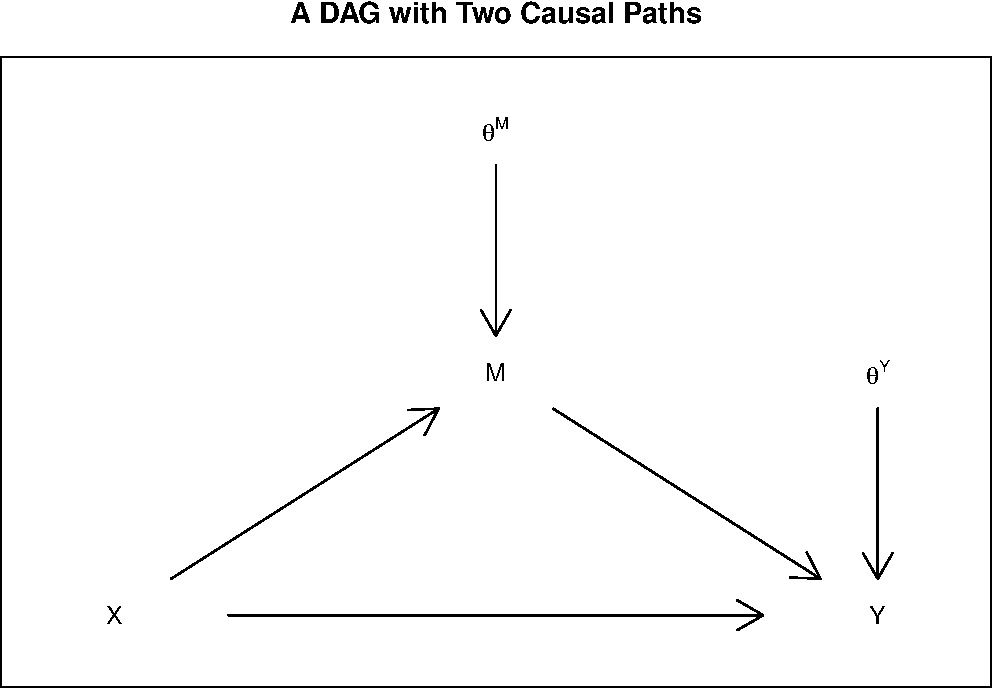
\includegraphics[width=0.6\linewidth]{ii_files/figure-latex/DAGpaths-1} 

}

\caption{Here $X$ has effects on $Y$ both indirectly through $M$ and directly.}\label{fig:DAGpaths}
\end{figure}

As we can show, we can define this causal-path query as a question about specific nodes on a causal graph. In particular, a causal path can be defined in terms of the values of \(\theta\) nodes: specifically, in the present example, in terms of \(\theta^M\) and \(\theta^Y\). To see why, let us first note that there are two combinations of effects that would allow \(X\)'s positive effect on \(Y\) to operate via \(M\): (1) \(X\) has a positive effect on \(M\), which in turn has a positive effect on \(Y\); or (2) \(X\) has a negative effect on \(M\), which has a negative effect on \(Y\).

Thus, in establishing whether \(X\) affects \(Y\) through \(M\), the first question is whether \(X\) affects \(M\) in this case. Whether or not it does is a question about the value of \(\theta^M\). We know that \(\theta^M\) can take on four possible values corresponding to the four possible responses to \(X\): \(\theta^M_{10}, \theta^M_{01}, \theta^M_{00}, \theta^M_{11}\). For sequence (1) to operate, \(\theta^M\) must take on the value \(\theta^M_{01}\), representing a positive effect of \(X\) on \(M\). For sequence (2) to operate, \(\theta^M\) must take on the value \(\theta^M_{10}\), representing a negative effect of \(X\) on \(M\).

\(\theta^Y\) defines \(Y\)'s response to different combinations of two other variables---here, \(X\) and \(M\)---since \emph{both} of these variables point directly into \(Y\). Where \(X\) can have both a mediated effect through \(M\) and a direct effect, \(X\) and \(M\) also potentially \emph{interact} in affecting \(Y\). Another way to think about this setup is that \(M\) is not just a possible mediator of \(X\)'s indirect effect; \(M\) is also a potential \emph{moderator} of \(X\)'s direct effect. This results in sixteeen possible values for \(\theta^Y\)---again as shown above in Table \ref{tab:PO16}.

What values of \(\theta^Y\)
then are compatible with the operation of the \(M\) causal path? Let us first consider this question with respect to sequence (1), in which \(X\) has a positive effect on \(M\), and that positive effect is necessary for \(X\)'s positive effect on \(Y\) to occur. For this sequence to operate, \(\theta^M\) must take on the value of \(\theta^M_{01}\). When it comes to \(\theta^Y\), then, what we need to look for types in which \(X\)'s effect on \(Y\) \emph{depends on \(M\)'s taking on the value it does as a result of \(X\)'s positive effect on \(M\)}.

We are thus looking for nodal types that capture two kinds of counterfactual causal relations operating on nodes. First, \(X\) must have a positive effect on \(Y\) when \(M\) changes as it does as a result of \(X\)'s positive effect on \(M\). Second, that change in \(M\), generated by a change in \(X\), must be \emph{necessary} for \(X\)'s positive effect on \(Y\) to operate. The thought experiment here thus imagines a situation in which \(X\) changes from \(0\) to \(1\),\footnote{This is the natural thought experiment when explaining a case with realized value of \(X=1\), in which the outcome can be thought of as having been generated by a change from \(X=0\). The identification of types does hinge, however, on the direction in which we imagine types changing. In other situations, we might observe \(X=Y=0\) and thus conceive of the outcome as having been generated by a change from \(X=1\) to \(X=0\) (again, assuming a positive effect of \(X\) on \(Y\)). When we do this, query 2 below changes: we are now looking for types in which \(Y=1\) when \(X=0\) but \(M=1\). (Does \(Y\) stay at \(1\) when \(X\) moves to \(0\) but \(M\) doesn't?) The queries are then satisfied by types \(6\) and \(8\), rather than \(2\) and \(6\).} but \(M\) does \emph{not} change to the value that it should as a result of this change in \(X\). We then inspect our types to see if \(Y\) would change from \(0\) to \(1\) in this situation. It is only if \(Y\) would \emph{not} change to \(1\) in this situation that we have identified a nodal type for which the \(M\)-mediated path matters. It is this thought experiment that isolates the causal significance of the path that runs through \(M\).

Assuming a positive effect of \(X\) on \(M\) (\(\theta^M=\theta^M_{01}\)), we thus need to apply the following set of queries to \(\theta^Y\):\footnote{Using standard potential outcomes notation, we can express the overall query, conditioning on a positive effect of \(X\) on \(M\), via the inequality \(Y(1, M(1)) - Y(0, M(0)) > Y(1, M(0)) - Y(0, M(0))\). The three specific queries formulated below simply correspond to the three unique elements of this expression. We can also readily map the path query that we are defining here---does the positive effect of \(X\) on \(Y\) depend on \(X\)'s effect on \(M\)---onto a query posed in terms of indirect effects. For instance, in our binary setup, conditioning our path query on a positive causal effect of \(X\) on \(Y\), a positive effect of \(X\) on \(M\), and an imagined change from \(X=0\) to \(X=1\) generates precisely the same result (identifies the same \(\theta^Y\) types) as asking which \(\theta^Y\) types are consistent with a positive indirect effect of \(X\) on \(Y\), conditioning on a positive total effect and \(X=1\).}

\begin{enumerate}
\def\labelenumi{\arabic{enumi}.}
\item
  Is \(X=1\) a counterfactual cause of \(Y=1\), given \(X\)'s positive effect on \(M\)? Establishing this positive effect of \(X\) involves two queries:

  \begin{enumerate}
  \def\labelenumii{\alph{enumii})}
  \item
    Where \(X=0\), does \(Y=0\)? As we are assuming \(X\) has a positive effect on \(M\), if \(X=0\) then \(M=0\) as well. We thus look down the \(X=0, M=0\) column and eliminate those types in which we do not observe \(Y=0\). This eliminates types \(9\) through \(16\).
  \item
    Where \(X=1\), does \(Y=1\)? Again, given \(X\)'s assumed positive effect on \(M\), \(M=1\) under this condition. Looking down the \(X=1, M=1\) column, we eliminate those types where we do not see \(Y=1\). We retain only types \(2, 4, 6,\) and \(8\).
  \end{enumerate}
\item
  Is \(X\)'s effect on \(M\) necessary for \(X\)'s positive effect on \(Y\)? That is, do we see \(Y=1\) \emph{only} if \(M\) takes on the value that \(X=1\) generates (\(M=1\))? To determine this, we inspect the \emph{counterfactual} condition in which \(X=1\) and \(M=0\), and we ask: does \(Y=0\)? Of the four remaining types, only \(2\) and \(6\) pass this test.
\end{enumerate}

Under these and only these two values of \(\theta^Y\)---\(\theta^Y_{0001}\) and \(\theta^Y_{0101}\)---we will see a positive effect of \(X\) on \(Y\) for which the \(M\)-mediated path is causally necessary, given a positve effect of \(X\) on \(M\). These two \(\theta^Y\) values are also different from one another in an interesting way. For type \(\theta^Y_{0101}\), \(X\)'s effect on \(Y\) runs strictly through \(M\): if \(M\) were to change from \(0\) to \(1\) \emph{without} \(X\) changing, \(Y\) would still change from \(0\) to \(1\). \(X\) is causally important for \(Y\) \emph{only} insofar as it affects \(M\). In a case of type \(\theta^Y_{0101}\), then, anything else that similarly affects \(M\) would generate the same effect on \(Y\) as \(X\) does. In type \(\theta^Y_{0001}\), however, both \(X\)'s change to \(1\) \emph{and} the resulting change in \(M\) are necessary to generate \(Y\)'s change to \(1\); \(X\)'s causal effect thus requires both the mediated and the unmediated pathway. And here \(X\) itself matters in the counterfactual sense; for a case of type \(\theta^Y_{0001}\), some other cause of \(M\) would \emph{not} generate the same effect on \(Y\).

We can undertake the same exercise for sequence (2), in which \(X\) first has a negative effect on \(M\), or \(\theta^M=\theta^M_{10}\). Here we adjust the three queries for \(\theta^Y\) to take account of this negative effect. Thus, we adjust query 1a so that we are looking for \(Y=0\) when \(X=0\) and \(M=1\). In query 1b, we look for \(Y=1\) when \(X=1\) and \(M=0\). And for query 2, we want types in which \(Y\) fails to shift to \(1\) when \(X\) shifts to \(1\) but \(M\) stays at \(1\). Types \(\theta_{0010}\) and \(\theta_{1010}\) pass these three tests.

In sum, we can define a query about causal paths as a query about the value of \(\theta\) terms on the causal graph. For the graph in Figure \ref{fig:DAGpaths}, asking whether \(X\)'s effect runs via the \(M\)-mediated path is asking whether one of four combinations of \(\theta^M\) and \(\theta^Y\) hold in case:

\begin{itemize}
\tightlist
\item
  \(\theta^M=\theta^M_{01}\) and (\(\theta^Y=\theta_{0001}\) or \(\theta_{0101}\))
\item
  \(\theta^M=\theta^M_{10}\) and (\(\theta^Y=\theta_{0010}\) or \(\theta_{1010}\))
\end{itemize}

It is worth noting how different this formulation of the task of identifying causal pathways is from widespread understandings of process tracing. Scholars commonly characterize process tracing as a method in which we determine whether a mechanism was operating by establishing whether the events lying along that path occurred. As a causal-model framework makes clear, finding out that \(M=1\) (or \(M=0\), for that matter) does not establish what was going on causally. Observing this intervening step does not by itself tell us what value \(M\) \emph{would} have taken on if \(X\) had taken on a different value, or whether this would have changed \(Y\)'s value. We need instead to conceive of the problem of identifying pathways as one of figuring out the \emph{counterfactual} response patterns of the variables along the causal chain. As we will demonstrate later in the book, explicitly characterizing those response patterns as nodes in a causal model helps us think systematically about empirical strategies for drawing the relevant inferences.

\hypertarget{general-procedure}{%
\section{General procedure}\label{general-procedure}}

We have been able to associate a collection of causal types to each of the causal queries we have described in this chapter. But we have not described a general method for doing so. We do that now.\footnote{In particular we describe the algorithm used by the \texttt{CausalQueries} package. This approach is not the efficient but it is intuitive and can be used for arbitrarily complex queries.}

The algorithm calculates the full set of outcomes on all nodes, given each possible causal type and a collection of controlled conditions (``\texttt{do} operations''). Then each causal type is marked as satisfying the query or not. This in turn then tells us the \emph{set} of types that satisfy a query. Quantitative queries, such as the probability of a query being satisfied, or the average treatment effect, can then be calculated by taking the measure of the set of causal types that satisfies the query.

First some notation.

Let \(n\) denote the number of nodes. Label the nodes \(V_1, \dots V_n\) subject to the requirement that each node's parents precede it in the ordering. Let \(pa_j\) denote the set of values of the parents of node \(j\) and let \(V_j(pa_j, \theta_t)\) denote the value of node \(j\) given the values of its parents and the causal type \(\theta_t\).

The primitives of a query are questions about the values of outcomes, \(V\), given some set of controlled operations \(x\).

\begin{itemize}
\tightlist
\item
  let \(x = (x_1, \dots x_n)\) denote a set of \texttt{do} operations where each \(x_i\) takes on a value in \(\{-1,0,1\}\). here -1 indicates ``not controlled'', 0 means set to 0 and 1 means set to 1 (this set can be expanded if \(V\) is not binary)
\item
  let \(V(x, \theta_t)\) denote the values \(V\) (the full set of nodes) takes given \(\theta_t\)
\item
  a ``simple query'' is a function \(q(V(x, \theta_t))\) which returns TRUE if \(V(x, \theta_t)\) satisfies some condition and FALSE otherwise.
\end{itemize}

Queries are summaries of simple queries. For instance, for nodes \(X\) and \(Y\):

\begin{itemize}
\tightlist
\item
  Query \(Q_1:\mathbb{1}(Y(X=1)=1))\) asks whether \(Y=1\) when \(X\) is set to 1. This requires evaluating one simple query.
\item
  Query \(Q_2:\mathbb{1}(Y(X=1)=1) \& \mathbb{1}(Y(X=0)=0))\) is composed of two simple queries: the first returns true if \(Y\) is 1 when \(X\) is set to 1, the second returns true if \(Y\) is 0 when \(X\) is set to 0; both conditions holding corresponds to a positive effect on a unit.
\item
  Query \(Q_3:E((\mathbb{1}(Y(X=1)=1) \& (Y(X=0)=0)) - (\mathbb{1}(Y(X=1)=0) \& \mathbb{1}(Y(X=0)=1))\) asks for the average treatment effect, represented here using four simple queries: the expected difference between positive and negative effects. This query involves weighting by the probability of the causal types.
\end{itemize}

Then to calculate \(V(x, \theta_t)\):

\begin{enumerate}
\def\labelenumi{\arabic{enumi}.}
\tightlist
\item
  Calculate \(v_1\), the realized value of the first node, \(V_1\), given \(\theta_t\). This is given by \(v_1 = x_1\) if \(x_1 \neq -1\) and by \(\theta_t^{V_1}\) otherwise.
\item
  For each \(j \in 2...n\) calculate \(v_j\) using either \(v_j = x_j\) if \(x_j \neq -1\) and \(V_{j}(pa_j, \theta_t)\) otherwise, where the values in \(pa_j\) are determined in the previous steps.
\end{enumerate}

We now have the outcomes, \(V\), for all nodes given the operations \(x\) and so can determine \(q(V(x))\). From there we can calculate summaries of simple queries across causal types.

A last note on conditional queries. Say we are interested in an attribution query of the form: what is the probability that \(X\) causes \(Y\) in a case in which \(X=1\) and \(Y=1\). In this case define simple query \(q_1\) which assesses whether \(X\) causes \(Y\) for a given \(\theta_t\) and simple query \(q_2\) which assesses whether \(X=1\) and \(Y=1\) under \(\theta_t\). We then calculate the conditional query by conditioning on the set of \(\theta\)s for which \(q_2\) is true and evaluating the share of these for which \(q_2\) is true (weighting by the probability of the causal types).

\hypertarget{chapter-appendix-1}{%
\section{Chapter Appendix}\label{chapter-appendix-1}}

We demonstrate how queries are calculated using the \texttt{CausalQueries} package for a chain model of the form \(X \rightarrow M \rightarrow Y\). We imagine a model of this form in which we assume no negative effects of \(M\) on \(X\) or \(M\) on \(Y\). We will also suppose that in fact \(X=1\), always. Doing this keeps the parameter space a little smaller for this demonstration but also serves to demonstrate that a causal model can make use of the counterfactual possibility that a node takes on a particular value even if it never does in fact.

We then ask two questions:

\begin{itemize}
\tightlist
\item
  Q1. What is the probability that \(X\) causes \(Y\)? (``POS'')
\item
  Q2. What is the probability that \(X\) causes \(Y\) in cases in which \(X=1\) and \(Y=1\)? (``POC'')
\end{itemize}

To answer these two queries we define simple query \(q_1\) which assesses whether \(X\) causes \(Y\) for each \(\theta\) and a second simple query \(q_2\) which assesses whether \(X=1\) and \(Y=1\) for each \(\theta\). In this example the first simple query involves some \texttt{do} operations, the second does not.

Code to answer these two simple queries is shown below and the output is shown in Table \ref{tab:ch4q1q2} (one row for each causal type).

\begin{Shaded}
\begin{Highlighting}[]
\NormalTok{model }\OtherTok{\textless{}{-}} \FunctionTok{make\_model}\NormalTok{(}\StringTok{"X {-}\textgreater{} M {-}\textgreater{} Y"}\NormalTok{) }\SpecialCharTok{\%\textgreater{}\%}
         \FunctionTok{set\_restrictions}\NormalTok{(}\StringTok{"X[]==0"}\NormalTok{) }\SpecialCharTok{\%\textgreater{}\%}
         \FunctionTok{set\_restrictions}\NormalTok{(}\StringTok{"M[X=1] \textless{} M[X=0]"}\NormalTok{) }\SpecialCharTok{\%\textgreater{}\%}
         \FunctionTok{set\_restrictions}\NormalTok{(}\StringTok{"Y[M=1] \textless{} Y[M=0]"}\NormalTok{)   }

\NormalTok{q1 }\OtherTok{\textless{}{-}} \StringTok{"Y[X = 1] \textgreater{} Y[X = 0]"}
\NormalTok{q2 }\OtherTok{\textless{}{-}} \StringTok{"X == 1 \& Y == 1"}

\NormalTok{df }\OtherTok{\textless{}{-}} \FunctionTok{data.frame}\NormalTok{(}
  \AttributeTok{a1 =}\NormalTok{ CausalQueries}\SpecialCharTok{:::}\FunctionTok{map\_query\_to\_causal\_type}\NormalTok{(model, q1)}\SpecialCharTok{$}\NormalTok{types,}
  \AttributeTok{a2 =}\NormalTok{ CausalQueries}\SpecialCharTok{:::}\FunctionTok{map\_query\_to\_causal\_type}\NormalTok{(model, q2)}\SpecialCharTok{$}\NormalTok{types,}
  \AttributeTok{p  =} \FunctionTok{get\_type\_prob}\NormalTok{(model))}
\end{Highlighting}
\end{Shaded}

\begin{table}

\caption{\label{tab:ch4q1q2}Set of causal types in the model that satisfy q1 and q2 along with the probability of the type.}
\centering
\begin{tabular}[t]{lllr}
\toprule
  & a1 & a2 & p\\
\midrule
\cellcolor{gray!6}{X1.M00.Y00} & \cellcolor{gray!6}{FALSE} & \cellcolor{gray!6}{FALSE} & \cellcolor{gray!6}{0.111}\\
X1.M01.Y00 & FALSE & FALSE & 0.111\\
\cellcolor{gray!6}{X1.M11.Y00} & \cellcolor{gray!6}{FALSE} & \cellcolor{gray!6}{FALSE} & \cellcolor{gray!6}{0.111}\\
X1.M00.Y01 & FALSE & FALSE & 0.111\\
\cellcolor{gray!6}{X1.M01.Y01} & \cellcolor{gray!6}{TRUE} & \cellcolor{gray!6}{TRUE} & \cellcolor{gray!6}{0.111}\\
\addlinespace
X1.M11.Y01 & FALSE & TRUE & 0.111\\
\cellcolor{gray!6}{X1.M00.Y11} & \cellcolor{gray!6}{FALSE} & \cellcolor{gray!6}{TRUE} & \cellcolor{gray!6}{0.111}\\
X1.M01.Y11 & FALSE & TRUE & 0.111\\
\cellcolor{gray!6}{X1.M11.Y11} & \cellcolor{gray!6}{FALSE} & \cellcolor{gray!6}{TRUE} & \cellcolor{gray!6}{0.111}\\
\bottomrule
\end{tabular}
\end{table}

The answer to the overall queries are then (1) the expected value of (the answers to) \(q_1\) and weights \(p\)and (2) the expected value of (the answers to) \(q_1\) given \(q_0\) and weights \(p\). See Table \ref{tab:ch4pospoc}.

\begin{Shaded}
\begin{Highlighting}[]
\NormalTok{df }\SpecialCharTok{\%\textgreater{}\%} \FunctionTok{summarize}\NormalTok{(}\AttributeTok{POS =} \FunctionTok{weighted.mean}\NormalTok{(a1, p),}
                 \AttributeTok{POC =} \FunctionTok{weighted.mean}\NormalTok{(a1[a2], p[a2]))}
\end{Highlighting}
\end{Shaded}

\begin{table}

\caption{\label{tab:ch4pospoc}Calculated answers to two queries.}
\centering
\begin{tabular}[t]{rr}
\toprule
POS & POC\\
\midrule
\cellcolor{gray!6}{0.111} & \cellcolor{gray!6}{0.2}\\
\bottomrule
\end{tabular}
\end{table}

Given the equal weighting on causal types, these answers reflect the fact that for 5 of 9 causal types we expect to see \(X=1\) and \(Y=1\) but that; the causal effect is present for only 1 of 9 causal types and for 1 of the 5 causal types that exhibit \(X=1\) and \(Y=1\).

\hypertarget{bayeschapter}{%
\chapter{Bayesian Answers}\label{bayeschapter}}

\begin{headerbox}
We run through the logic of Bayesian updating and show how it is used for answering causal queries. We illustrate with applications to correlational and process tracing inferences.

\end{headerbox}

Bayesian methods are just sets of procedures to figure out how to update beliefs in light of new information.

We begin with a prior belief about the probability that a hypothesis is true. New data then allow us to form a posterior belief about the probability of the hypothesis. Bayesian inference takes into account the consistency of the evidence with a hypothesis, the uniqueness of the evidence to that hypothesis, and background knowledge about the problem.

In the next section we review the basic idea of Bayesian updating. The following section applies it to the problem of updating on causal queries given a causal model and data.

\hypertarget{bayes-basics}{%
\section{Bayes Basics}\label{bayes-basics}}

For simple problems, Bayesian inference accords well with our intuitions. Once problems get slightly more complex however, our intuitions often fail us.

\hypertarget{simple-instances}{%
\subsection{Simple instances}\label{simple-instances}}

Say I draw a card from a deck. The chances it is a Jack of Spades is just 1 in 52. If I tell you that the card is indeed a spade and asked you now what are the chances it is a Jack of Spades, you should guess 1 in 13. If I told you it was a heart you should guess there is no chance it is a Jack of Spades. If I said it was a face card and a spade you should say 1 in 3.

All those answers are applications of Bayes' rule. In each case the answer is derived by assessing what is possible, given the new information, and then assessing how likely the outcome of interest among the states that are possible. In all the cases you calculate:

\[\text{Prob Jack of Spades | Info} = \frac{\text{Is Jack of Spades Consistent with Info?}}{\text{How many cards are consistent with Info?}}\]

The same logic goes through when things are not quite so black and white.

Now consider two slightly trickier examples.

\textbf{Interpreting Your Test Results}. Say that you take a test to see whether you suffer from a disease that affects 1 in 100 people. The test is good in the sense that if you have the disease it will say you have it with a 99\% probability. If you do not have it, then with a 99\% probability, it will say that you do not have it. The test result says that you have the disease. What are the chances you have it? You might think the answer is 99\%, but that would be to mix up the probability of the result given the disease with the probability of the disease given the result. In fact the right answer is 50\%, which you can think of as the share of people that have the disease among all those that test positive. The logic is most easily seen if you think through it using frequencies (see \citet{hoffrage1998using} for this problem and ways to address it). If there were 10,000 people, then 100 would have the disease and 99 of these would test positive. But 9,900 would not have the disease and 99 of these would test positive. So the people with the disease that test positive are half of the total number testing positive.

As an equation this might be written:

\begin{align*} 
\text{Probability Sick | Test} &=& \frac{\text{How many sick and test positive?}}{\text{How many test positive?}}\\ 
&=& \frac{99}{99 + 99}
\end{align*}

\textbf{Two-Child Problem} Consider last an old puzzle described in \citet{gardner1961second}. \emph{Mr Smith has two children, \(A\) and \(B\). At least one of them is a boy. What are the chances they are both boys?}
To be explicit about the puzzle, we will assume that the information that one child is a boy is given as a truthful answer to the question ``is at least one of the children a boy?'' Assuming that there is a 50\% probability that a given child is a boy, people often assume the answer is 50\%. But surprisingly the answer is 1 in 3. The information provided rules out the possibility that both children are girls and so the right answer is found by readjusting the probability that two children are boys based on this information. As an equation:

\begin{align*} 
\text{Probability both boys | Not both girls} &=& \frac{\text{Probability  both boys}}{\text{Probability not both girls}} \\ 
&=& \frac{\text{1 in 4}}{\text{3 in 4}}
\end{align*}

\hypertarget{bayes-rule-for-discrete-hypotheses}{%
\subsection{Bayes' Rule for Discrete Hypotheses}\label{bayes-rule-for-discrete-hypotheses}}

Formally, all of these equations are applications of Bayes' rule which is a simple and powerful formula for deriving updated beliefs from new data.

The formula is given as:

\begin{align}
\Pr(H|\mathcal{D})&=\frac{\Pr(\mathcal{D}|H)\Pr(H)}{\Pr(\mathcal{D})}\\
                  &=\frac{\Pr(\mathcal{D}|H)\Pr(H)}{\sum_{H'}\Pr(\mathcal{D}|H')\Pr(H'))}
\end{align}

where \(H\) represents a hypothesis, \(\mathcal{D}\) represents a particular realization of new data (e.g., a particular piece of evidence that we might observe), and the summation runs over an exhaustive and exclusive set of hypotheses.

Looking at the formula we see that the posterior belief derives from three considerations.

First the strength of our prior level of confidence in the hypothesis, \(\Pr(H)\). The greater the prior likelihood that our hypothesis is true, the greater the chance that new data consistent with the hypothesis has \emph{in fact} been generated by a state of the world implied by the hypothesis.

Second, the likelihood: how likely are we to have observed these data if the hypothesis were true, \(\Pr(\mathcal{D}|H\))?

Third, the probability of the data---the denominator. How likely are we to have observed these data regardless of whether the hypothesis is true or false, \(\Pr(\mathcal{D})\)?

The last two quantities capture how consistent the data are with our hypothesis and how specific the data are to our hypothesis. As shown in the equation above, the third quantity can usefully be written in terms of the different ways (alternative Hypotheses, \(H'\)) that the data could come about.

Note that answering the third question requires putting prior probabilities on an exclusive and exhaustive set of hypotheses. However, it does not require a listing of all possible hypotheses, just some exhaustive collection of hypotheses. For example we might have the notion of the probability that the accused's fingerprints would be on the door if she were or were not guilty without having to decompose the ``not guilty'' into a set of hypotheses regarding who else might be guilty. Also, while the hypotheses that enter the formula do have to be mutually exclusive, that does not prevent you from drawing inferences about hypotheses that are not mutually exclusive. For instance you might form posteriors over which of 100 people is guilty, but then use the posterior to ask what is the probability that a man is guilty, or that an old person is guilty. The fact that ``man'' and ``old'' are not mutually exclusive in no way means you cannot try to learn about both of these hypotheses.

\hypertarget{bayes-rule-for-continuous-parameters-and-the-dirichlet-family}{%
\subsection{Bayes' Rule for Continuous Parameters and The Dirichlet family}\label{bayes-rule-for-continuous-parameters-and-the-dirichlet-family}}

This basic formula extends in a simple way to collections of continuous variables. For example, say we are interested in the value of some parameter vector \(\theta\) (as a vector, \(\theta\) can contain many quantities we are uncertain about), we can calculate this, given a prior probability distribution over possible values of \(\theta\), \(p\), and given data \(D\) as:

\[p(\theta|\mathcal{D})=\frac{p(\mathcal{D}|\theta)p(\theta)}{\int_{\theta'}p(\mathcal{D|\theta'})p(\theta')d\theta}\]

Bayes rule requires the ability to express a prior distribution but it does not require that the prior have any particular properties other than being probability distributions.

In practice however when we are dealing with continuous parameters, it can be useful to make use of ``off the shelf'' distributions.

For the framework developed in this book, we will often be interested in forming beliefs about the \emph{share} of units that are of a particular type. For this type of question we will make quite heavy use of ``Dirichlet'' distributions: a family of distributions that capture beliefs about shares.

Consider, for example, the share of people in a population that voted; this is a quantity between 0 and 1. Two people might both believe that the turnout was around 50\% but may differ in how certain they are about this claim. One might claim to have no information and to believe that any turnout rate between 0 and 100\% is equally likely, giving an expected turnout of 50\%; another might be completely confident that the number is 50\% and entertain no other possibilities.

We can capture such beliefs quite well by using the Beta distribution---a special case of the Dirichlet. The Beta is a distribution over the \([0,1]\) that is governed by two parameters , \(\alpha\) and \(\beta\). In the case in which both \(\alpha\) and \(\beta\) are 1, the distribution is uniform---all values are considered equally likely. As \(\alpha\) rises large outcomes are seen as more likely and as \(\beta\) rises, lower outcomes are considered more likely. If both rise proportionately the expected outcome does not change but the distribution becomes tighter.

An attractive feature of the Beta distribution is that if one has a prior Beta (\(\alpha\), \(\beta\)) over the probability of some event (e.g.~that a coin comes up heads), and then one observes a positive case, the Bayesian posterior distribution is also a Beta with parameters \(\alpha+1, \beta\). Thus in a sense if people start with uniform priors and build up knowledge on seeing outcomes, their posterior beliefs should be Beta distributions.

Figure \ref{fig:Betas} shows a set of such distributions, starting with one that has greater variance than uniform (with alpha and beta both set to 0.5 this corresponds to the non informative ``Jeffrey's prior''), and including the uniform case (both alpha and beta set to 1), then cases in which multiple negative and positive outcomes have been seen.

\begin{figure}

{\centering 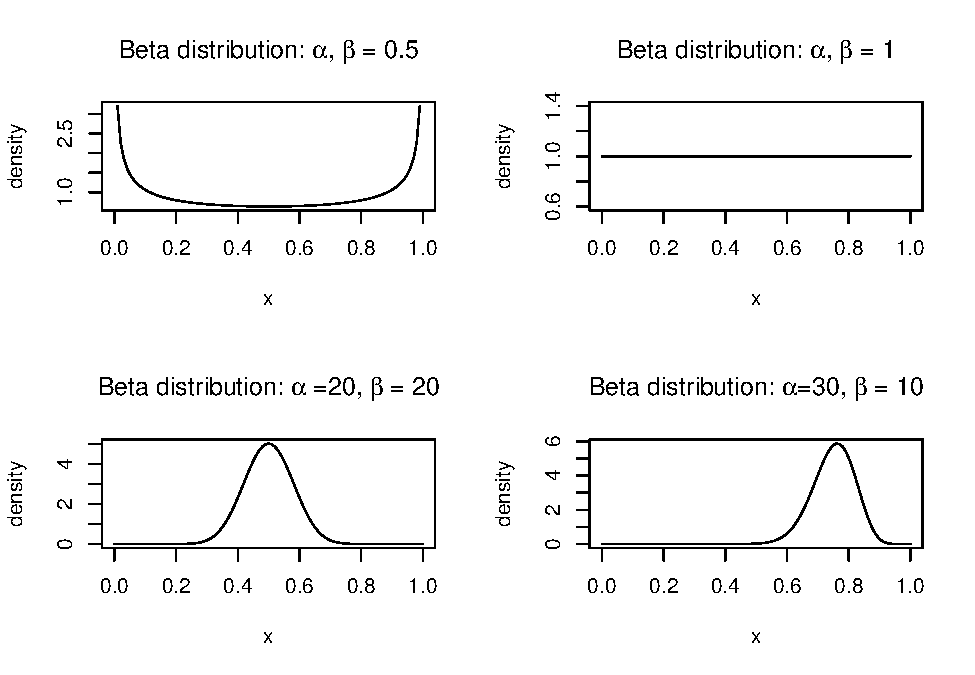
\includegraphics{ii_files/figure-latex/Betas-1} 

}

\caption{Beta distributions}\label{fig:Betas}
\end{figure}

Dirichlet distributions generalize the Beta to the situation in which there are beliefs not just over a proportion, or a probability, but over collections of probabilities. For example, if four outcomes are possible and each is likely to occur with probability \(\theta_k\), \(k=1,2,3,4\), then beliefs about these probabilities are distributions over a three-dimensional unit simplex---that is, all 4 element vectors of probabilities that add up to 1. The distribution has as many parameters as there are outcomes and these are traditionally recorded in a vector, \(\alpha\). Similar to the Beta distribution, an uninformative prior (Jeffrey's prior) has \(\alpha\) parameters of \((.5,.5,.5, \dots)\) and a uniform (``flat'') distribution has \(\alpha = (1,1,1,,\dots)\).

As with the Beta distribution, the Dirichlet updates in a simple way. If you have a Dirichlet prior with parameter \(\alpha = (\alpha_1, \alpha_2, \dots)\) and you observe outcome \(1\), for example, then then posterior distribution is also Dirichlet with parameter vector \(\alpha' = (\alpha_1+1, \alpha_2,\dots)\).

\hypertarget{moments}{%
\subsection{Moments}\label{moments}}

In what follows we often refer to the ``posterior mean'' or the ``posterior variance.'' These are simply summary statistics of the posterior distribution, or moments, and can be calculated easily once the posterior is known. For example the posterior mean of a parameter \(\theta_1\)---just one in a collection of parameters stored in \(\theta\)---is simply \(\overline{\theta}_1 | \mathcal{D} = \int \theta_1 p(\theta | \mathcal{D}) d\theta\). Note importantly that this is calculated using the posterior over the entire vector \(\theta\). Similarly the posterior variance is \(\int (\theta_1 - (\overline{\theta}_1 | \mathcal{D})^2 p(\theta | \mathcal{D})) d\theta\).

\hypertarget{bayes-estimation-in-practice}{%
\subsection{Bayes estimation in practice}\label{bayes-estimation-in-practice}}

Although the principle of Bayesian inference is quite simple, in practice calculating posteriors for continuous parameters is computationally complex.

In principle, with continuous parameters there is an infinity of possible parameter values. Analytic solutions are not, in general, easy to come by and so researchers use some form of sampling.

Imagine for instance you were interested in forming a posterior on the share of U.S. voters intending to vote Democrat, given polling data. (This is not truly continuous, but with large elections it might as well be.)

One approach is to coarsen the parameter space: we calculate the probability of observing the polling data given possible values \(\theta = 0, \theta = .1, \theta = .2, \dots, \theta = 1\), and, apply Bayes rule to form a posterior for each of these possibilities. The downside of the this approach is that, for a decent level of precision, it becomes computationally expensive with large parameter spaces, and parameter spaces get large quickly. For instance, if we are interested in vote shares, we might find .4, .5, and .6 too coarse and want posteriors for 0.51 or even 0.505; the latter would require calculations for 200 parameter values. If we had \emph{two} parameters that we wanted to slice up each into 200 possible values, we would then have 40,000 parameter pairs to worry about. What's more, \emph{most} of those calculations would not be very informative if the real uncertainty all lies in some small (though possibly unknown) range---such as between 40\% and 60\%.

An alternative approach is to use variants of Markov Chain Monte Carlo sampling. Under these approaches, parameter vectors are sampled and their likelihood is evaluated. If a sampled parameter vector is found to have high likelihood, then new parameter vectors near it are drawn with a high probability. Based on the likelihood associated with these new draws, additional draws are made. The result is a chain of draws that build up to approximate the posterior distribution. The output from these procedures is not a set of probabilities for each possible parameter vector but rather a set of draws of parameter vectors from the posterior distribution.

Many algorithms have been developed to achieve these tasks efficiently; in all of our applications we rely on the \texttt{stan} procedures which use MCMC methods, specifically the Hamiltonian Monte Carlo (HMC) algorithm and the no-U-turn sampler (NUTS). Details on these approaches are given in the \href{https://mc-stan.org/docs/2_18/reference-manual/hmc-chapter.html}{Stan Reference Manual} \citep{stan2020stan}.

\hypertarget{bayes-applied}{%
\section{Bayes applied}\label{bayes-applied}}

\hypertarget{simple-bayesian-process-tracing}{%
\subsection{Simple Bayesian Process Tracing}\label{simple-bayesian-process-tracing}}

Process tracing in its most basic form seeks to use within-case evidence to draw inferences about a case. For example, with a focus on whether \(X\) caused \(Y\), data on a within-case ``clue'', \(K\), is used to make inference about whether or not the outcome in that case was generated by the case's treatment status on \(X\). We refer to the within-case evidence gathered during process tracing as \emph{clues} in order to underline their probabilistic relationship to the causal relationship of interest. Readers familiar with the framework in \citet{collier2004sources} can usefully think of our ``clues'' as akin to causal process observations, although we highlight that there is no requirement that the clues be generated by the causal process.

To make inferences, the analyst looks for clues that will be observed with some probability if the case is of a given type and that will \emph{not} be observed with some probability if the case is \emph{not} of that type.

It is relatively straightforward to express the logic of process tracing in Bayesian terms, a step that will aid the integration of qualitative with quantitative causal inferences. As noted by others (e.g. \citet{BennettBayes}, \citet{beachpedersen2013process}, \citet{rohlfing2012case}), there is an evident connection between the use of evidence in process tracing and Bayesian inference. See \citet{fairfield2017explicit} for a detailed treatment of Bayesian approach in qualitative research.

To illustrate, suppose we are interested in regime collapse. We already have \(X,Y\) data on one authoritarian regime: we know that it suffered economic crisis (\(X=1\)) and collapsed (\(Y=1\)). We want to know what caused the collapse. To make progress we will try to draw inferences given a ``clue.'' Beliefs about the probabilities of observing clues for cases with different causal effects derive from theories of, or evidence about, the causal process connecting \(X\) and \(Y\). Suppose we theorize that the mechanism through which economic crisis generates collapse runs via diminished regime capacity to reward its supporters during an economic downturn. A possible clue to the operation of a causal effect, then, might be the observation of diminishing rents flowing to regime supporters shortly after the crisis. If we believe the theory, then this is a clue that we might believe to be highly probable for cases of type \(b\) that have experienced economic crisis (where the crisis in fact caused the collapse) but of low probability for cases of type \(d\) that have experienced crisis (where the collapse occurred for other reasons).

To make use of Bayes rule we need to:

\begin{enumerate}
\def\labelenumi{\arabic{enumi}.}
\tightlist
\item
  define our parameters, which are the key quantities of interest
\item
  provide prior beliefs about the parameters of interest
\item
  define a likelihood function
\item
  provide the probability of the data
\item
  plug these into Bayes' rule to calculate a posterior on the parameters of interest
\end{enumerate}

We discuss each of these in turn, using our \(a, b, c, d\) type notation for simplicity.

\textbf{Parameters.} The inferential challenge is to determine whether the regime collapsed \emph{because} of the crisis (it is \(b\) type) or whether it would have collapsed even without it (\(d\) type). We do so using further information from the case---one or more clues. We use the variable \(K\) to register the outcome of the search for a clue, with \(K\)=1 indicating that a specific clue is searched for and found, and \(K\)=0 indicating that the clue is searched for and not found.

Let \(j\in \{a,b,c,d\}\) refer to the type of an individual case. Our hypothesis, in this initial setup, consists simply of a belief about \(j\) for the case under examination: specifically whether the case is a \(b\) type (\(j=b)\). The parameter of interest is the causal type.

\textbf{Prior.} We then assign a prior degree of confidence to the hypothesis (\(p = Pr(H)\)). This is, here, our prior belief that an authoritarian regime that has experienced economic crisis is a \(b\).

\textbf{Likelihood.} The likelihood, \(\Pr(K=1|H)\) is the probability of observing the clue, when we look for it in our case, if the hypothesis is true---i.e., here, if the case is a \(b\) type. The key feature of a clue is that the probability of observing the clue is believed to depend on the case's causal type. In order to calculate the probability of the data we will in fact need two such probabilities: we let \(\phi_b\) denote the probability of observing the clue for a case of \(b\) type (\(\Pr(K=1|j=b)\)), and \(\phi_d\) the probability of observing the clue for a case of \(d\) type (\(\Pr(K=1|j=d)\)). The key idea in many accounts of process tracing is that the \emph{differences} between these probabilities provides clues with `'probative value,'' that is, the ability to generate learning about causal types. The likelihood, \(\Pr(K=1|H)\), is simply \(\phi_b\).

\textbf{Probability of the data.} This is the probability of observing the clue when we look for it in a case, \emph{regardless} of its type, \((\Pr(K=1))\). More specifically, it is the probability of the clue in a treated case with a positive outcome. As such a case can only be a \(b\) or a \(d\) type, this probability can be calculated simply from \(\phi_b\) and \(\phi_d\), together with our beliefs about how likely an \(X=1, Y=1\) case is to be a \(b\) or a \(d\) type.
This probability aligns (inversely) with Van Evera's concept of `'uniqueness.''

\textbf{Inference.} We can now apply Bayes' rule to describe the learning that results from process tracing. If we observe the clue when we look for it in the case, then our \emph{posterior} belief in the hypothesis that the case is of type \emph{b} is:

\[\Pr(j = b |K=1, X=Y=1)=  \frac{\phi_b p }{\phi_b p+\phi_d (1-p)}\]

In this exposition we did not make use of a causal model in a meaningful way---we simply need the priors and the clue probabilities.

In fact, however, these numbers can be derived from a causal model. To illustrate, imagine a simple causal model in which the \(X, Y\) relationship is completely mediated by \(K\). In particular, suppose, from background knowledge of the conditional distribution of outcomes given their causes, we have that:

\begin{itemize}
\tightlist
\item
  \(\Pr(K=1 | X=0) = 0\), \(\Pr(K=1 | X=1) = .5\)
\item
  \(\Pr(Y=1 | K=0) = .5\), \(\Pr(Y=1 | K=1) = 1\)
\end{itemize}

This data is consistent with a world in which half \(b\) and \(c\) types in the first step and half \(b\) and \(d\) types in the second step. Assume that the case at hand is sampled from this world.

Then we can calculate that the prior probability, \(p\), that \(X\) caused \(Y\) given \(X=Y=1\) is \(p = \frac13\).\footnote{Given \(X=1\), \(Y=1\) is consistent with \(b\) types at both stages, which arises with probability .25, or with a \(d\) type in the second stage, which arises with probability .5. The conditional probability is therefore \(.25/.75 = 1/3\).} We can also calculate the probability that \(K=1\) for a treated \(b\) and \(d\) case respectively as \(\phi_b=1\) and \(\phi_d=0.5\) (convince yourself of these numbers!). We then get:

\[\Pr(j = b |K=1, X=Y=1)=\frac{1\times \frac13}{1 \times \frac13 + 0.5 \times \frac23}=0.5\]

We thus shift our beliefs from a prior of \(\frac13\) to a posterior of \(\frac12\). In contrast had we \emph{not} observed the clue our posterior would have been 0.\footnote{We develop these ideas in more detail in Chapter \ref{justifying}.}

As should be clear from the above, the inferential leverage in process tracing comes from differences in the probability of observing \(K=1\) for different causal types. Thus, the logic described here generalizes Van Evera's familiar typology of tests by conceiving of the certainty and uniqueness of clues as lying along a continuum.

Van Evera's four tests (``smoking gun,'' ``hoop,'' ``straw in the wind,'' and ``doubly decisive'') represent, in this sense, special cases---particular regions that lie on the boundaries of a ``probative-value space.'' To illustrate the idea, we represent the range of combinations of possible probabilities for \(\phi_b\) and \(\phi_d\) as a square in Figure \ref{fig:CluesInferences1} and mark the spaces inhabited by Van Evera's tests. As can be seen, the type of test involved depends on both the relative \emph{and} absolute magnitudes of \(\phi_b\) and \(\phi_d\). The probative value of a test depends on the difference between them. Thus, a clue acts as a smoking gun for proposition ``\(b\)'' (the proposition that the case is a \(b\) type) if it is highly unlikely to be observed if proposition \(b\) is false, and more likely to be observed if the proposition is true (bottom left, above diagonal). A clue acts as a ``hoop'' test if it is highly likely to be found if \(b\) is true, even if it still quite likely to be found if it is false. Doubly decisive tests arise when a clue is very likely if \(b\) and very unlikely if not. It is, however, also easy to imagine clues with probative qualities lying in the large space amidst these extremes.\footnote{We thank Tasha Fairfield for discussions around this graph which differs from that in \citet{humphreys2015mixing} by placing tests more consistently on common rays originating from (0,0) and (1,1).}

\begin{figure}

{\centering 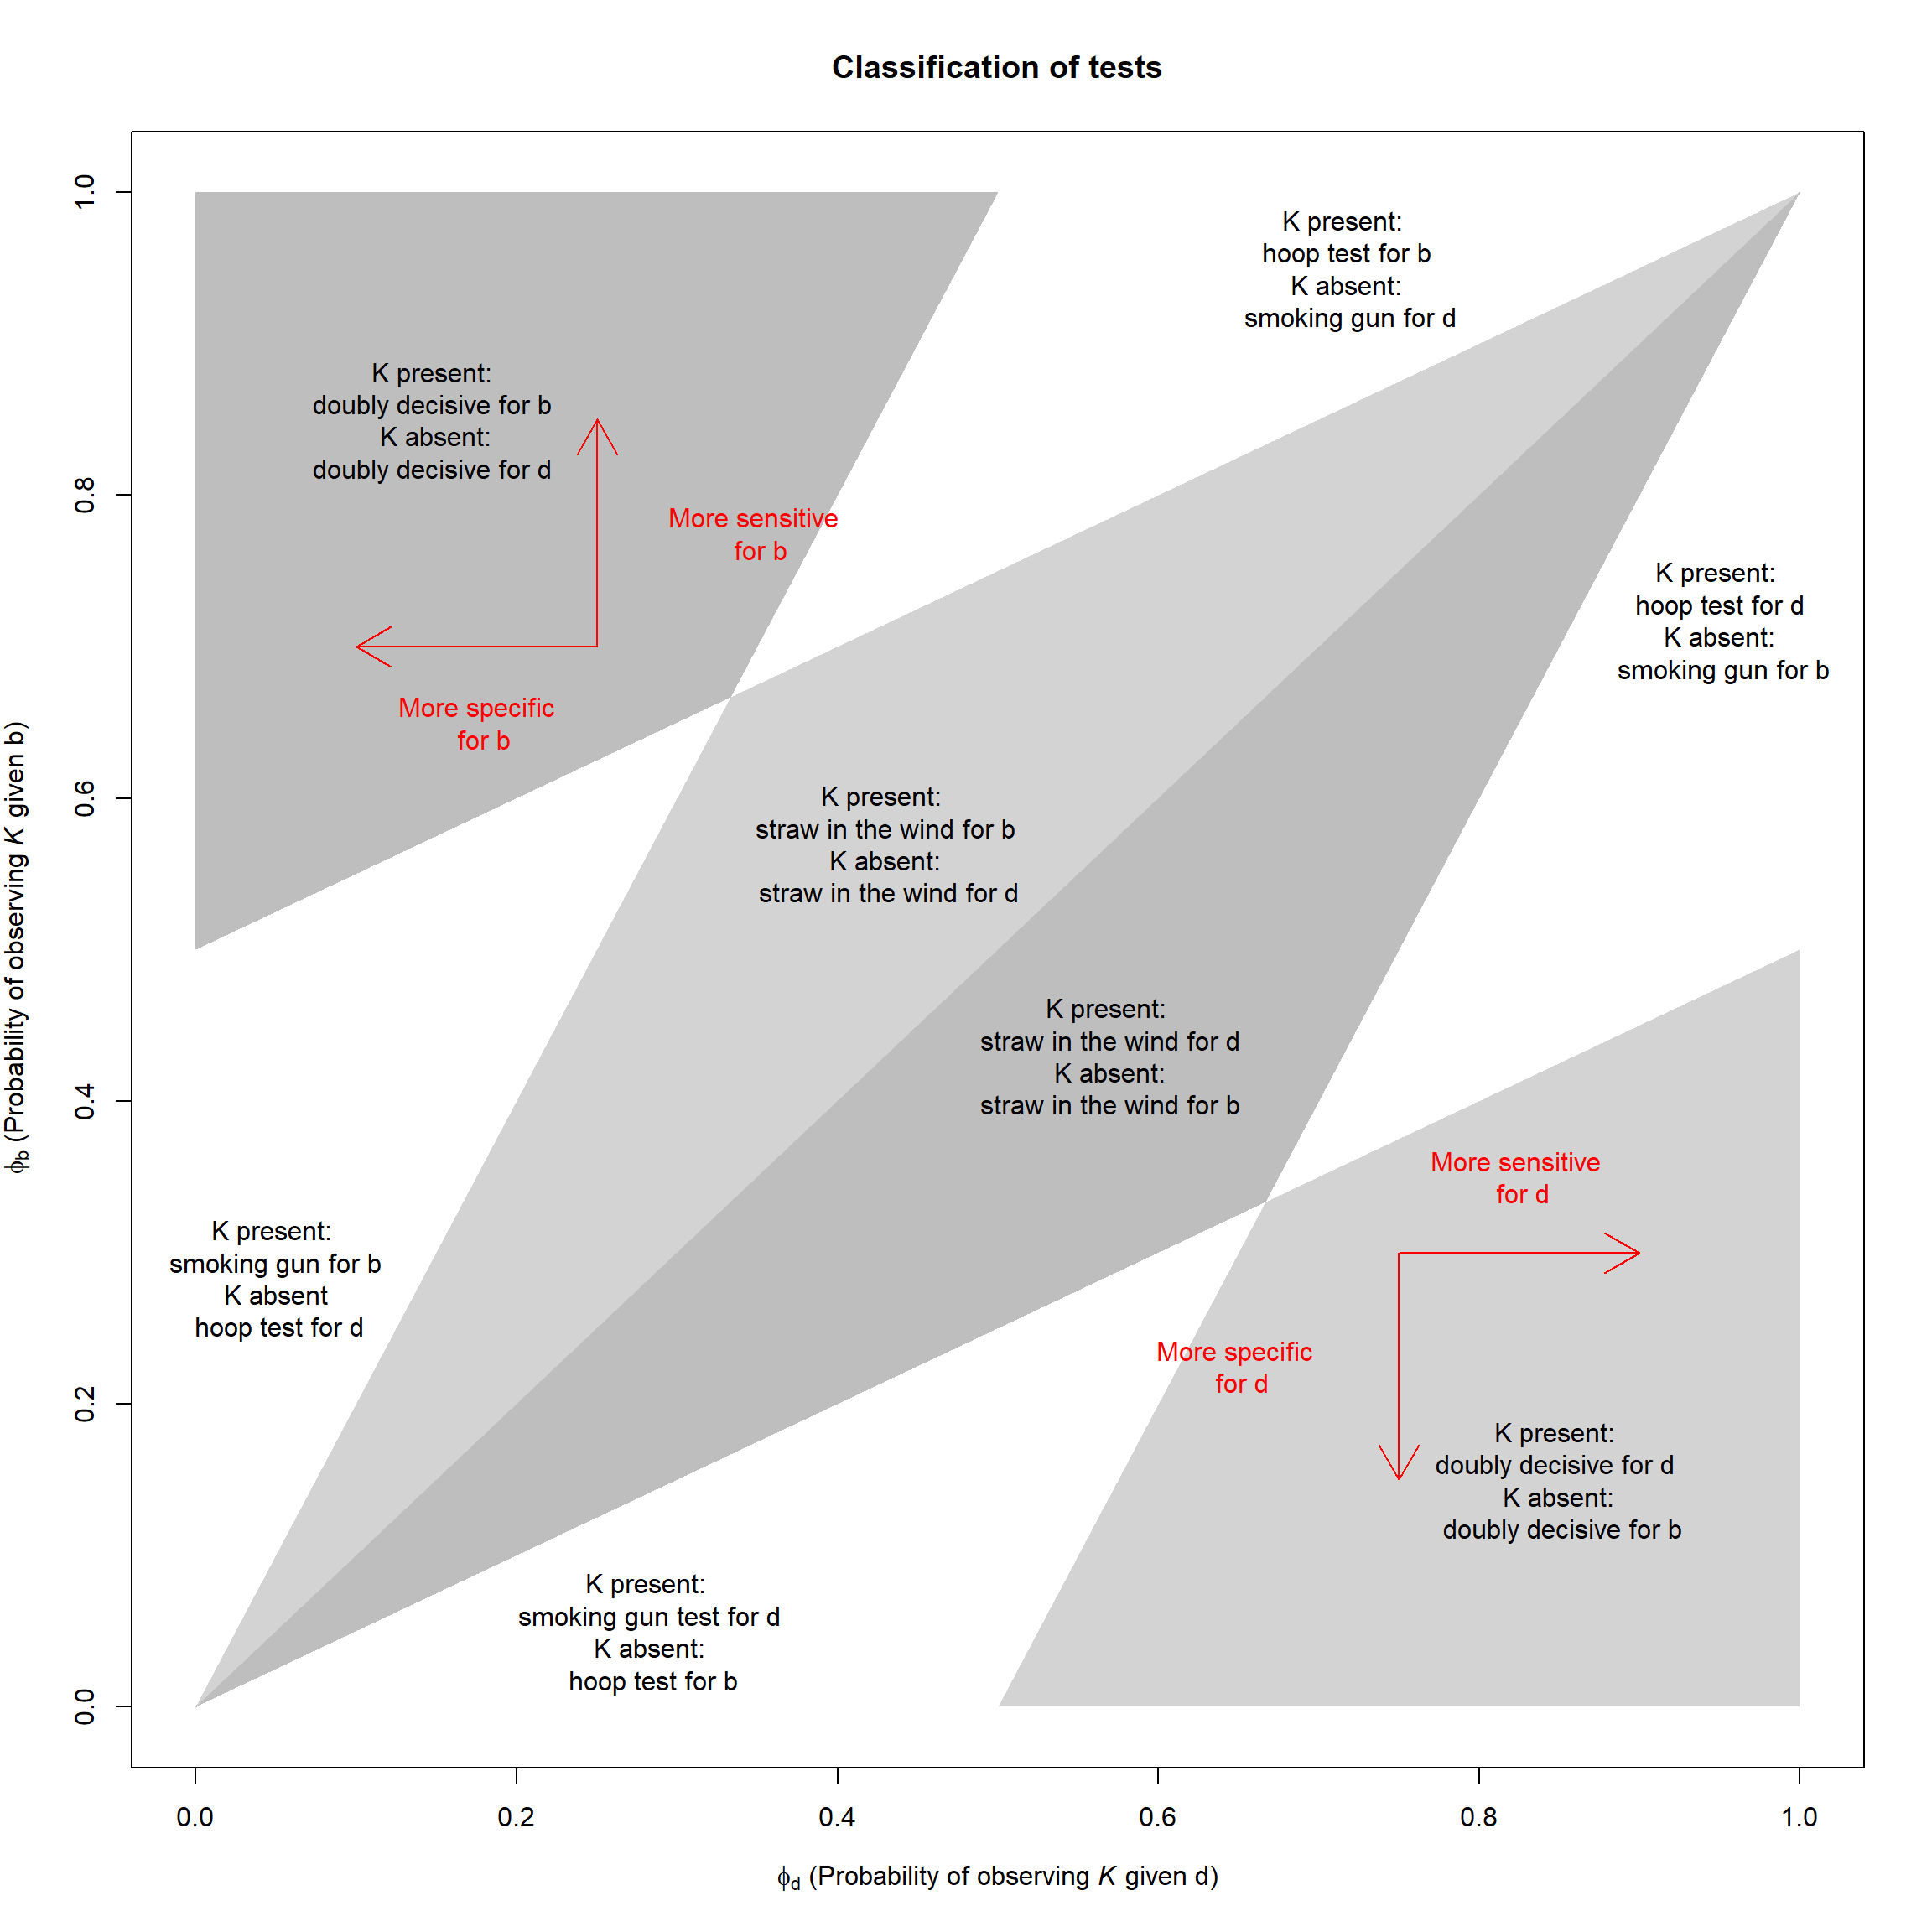
\includegraphics{ii_files/figure-latex/CluesInferences1-1} 

}

\caption{A mapping from the probability of observing a clue if the proposition that a case is a $b$ type is true ($\phi_b$) or false ($\phi_d$) to a generalization of the tests described in Van-Evera (1997).}\label{fig:CluesInferences1}
\end{figure}

In this illustration, we note that we draw both the priors and the probative value from a causal model. If we altered the model---for example, if we had a stronger first stage and so a larger value for \(\Pr(K=1|X=0)\)---this would alter both our prior, \(p\), and our calculations of \(\phi_d\). An implication of this is that, although one might be tempted to think of the priors and the probative values as independent quantities, and contemplate how inferences change as priors change (as we did for example in the treatment in \citet{humphreys2015mixing}), keeping probative value fixed, that kind of thought experiment may assume values that are not justified by an underlying model.

\hypertarget{a-generalization-bayesian-inference-on-queries}{%
\subsection{A Generalization: Bayesian Inference on Queries}\label{a-generalization-bayesian-inference-on-queries}}

In Chapter \ref{questions}, we described queries of interest as queries over nodal types in causal models.

Once queries are defined in terms of nodal types, the formation of beliefs, given data \(W\), about queries follows immediately from application of Bayes rule.

Let \(q(\theta)\) define the value of the query in context \(\theta\). The updated beliefs about the query are given by the distribution:

\[p(q' | W) = \int_{\theta:q(\theta) = q'} p(\theta|W)d\theta =  \int_{\theta:q(\theta) = q'} \frac{p(W|\theta)p(\theta)}{\int_{\theta'}p(W|\theta')p(\theta')d\theta'}d\theta\]

This expression gathers together all the causal types (combinations of nodal types) that satisfy a query and assesses how likely these are, collectively, given the data.\footnote{Learning about roots from observed data is sometimes termed \emph{abduction}; see \citet{pearl2009causality}, p 206.} For an abstract representation of the relations between assumptions, queries, data, and conclusions, see Figure 1 in \citet{pearl2012causal}.

Return now to Mr Smith's puzzle. We can think of the two ``nodal types'' here as the sexes of the two children, child \(A\) and child \(B\). The query here is \(q\): ``Are both boys?'' The statement ``\(q=1\)'' is equivalent to the statement, \(A\) is a boy \& \(B\) is a boy. Thus it takes the value \(q=1\) under just one causal type, when both nodes have been assigned to the value ``boy.'' Statement \(q=0\) is the statement (``\(A\) is a boy \& \(B\) is a girl'' or ``\(A\) is a girl \& \(B\) is a boy'' or ``\(A\) is a girl \& \(B\) is a girl''). Thus \(q=0\) in three contexts. If we assume that each of the two children is equally likely to be a boy or a girl with independent probabilities, then each of the four contexts is equally likely.
The result can then be figured out as \(p(q=1) = \frac{1\times \frac{1}{4}}{1\times \frac{1}{4} + 1\times \frac{1}{4}+1\times \frac{1}{4}+0\times \frac{1}{4}} = \frac{1}{3}\). This answer requires summing over only one causal type. \(p(q=0)\) is of course the complement of this, but using the Bayes formula one can see that it can be found by summing over the posterior probability of three causal types in which the statement \(q=0\) is true.

We will often want to think about our causal queries being collections of states of the world---i.e., of causal types. Returning to our discussion of queries in Chapter \ref{questions}, suppose we start with the model \(X \rightarrow M \rightarrow Y\), and our query is whether \(X\) has a positive effect on \(Y\). This is a query that is satisfied by four sets of causal types: those in which \(X\) has a positive effect on \(M\) and \(M\) has a positive effect on \(Y\), with \(X\) being either 0 or 1; and those in which \(X\) has a negative effect on \(M\) and \(M\) has a negative effect on \(Y\), with \(X\) being either 0 or 1. Our inferences on the query will thus involve gathering these different causal types, and their associated posterior probabilities, together.

One way to think intuitively about Bayesian updating is to say that we update more strongly in favor of the hypothesis for which the evidence is \emph{least} damaging to the \emph{most-likely ways} in which the hypothesis could be true. Suppose our prior belief was that it was much more unlikely that \(M\) had a negative effect on \(Y\), than that \(M\) had a positive effect on \(Y\). This makes one of the ways in which \(X\) could have a positive effect on \(Y\) (the chain of negative effects) much less likely than the other way in which \(X\) could have a positive effect on \(Y\) (the chain of positive effects). This means that evidence against a chain of negative effects and evidence against a chain of positive effects will not be equally consequential for our query: in particular, we will update more strongly against the query if we find evidence against a chain of positive effects than if we find evidence against a chain of negative effects. Evidence against a chain of positive effects speaks against the \emph{most} likely way in which the query could be true, whereas evidence against a chain of negative effects speaks against a way the query could be true that we did not think was very likely to begin with.

\hypertarget{features-of-bayesian-updating}{%
\section{Features of Bayesian updating}\label{features-of-bayesian-updating}}

Bayesian updating has implications that may not be obvious at first glance. These will matter for all forms of inference we examine in this book, but they can all be illustrated in simple settings.

\hypertarget{AppPriors}{%
\subsection{Priors matter}\label{AppPriors}}

The amount of learning that results from a given piece of new data depends strongly on prior beliefs. We have already seen this with the example of interpreting our test results above. Figure \ref{fig:CluesInferences2} illustrates the point for process tracing inferences.

In each subgraph of Figure \ref{fig:CluesInferences2} , we show how much learning occurs under different scenarios. The horizontal axis indicates the level of prior confidence in the hypothesis and the curve indicates the posterior belief that arises if we do (or do not) observe the clue. As can be seen, the amount of learning that occurs---the shift in beliefs from prior to posterior---depends a good deal on what prior we start out with. For a smoking gun test, the amount of learning is highest for values roughly in the 0.2 to 0.4 range---and then declines as we have more and more prior confidence in our hypothesis. For a hoop test, the amount of learning when the clue is \emph{not} observed is greatest for hypotheses in which we have middling-high confidence (around 0.6 to 0.8), and minimal for hypotheses in which we have a very high or a very low level of confidence.

\begin{figure}

{\centering 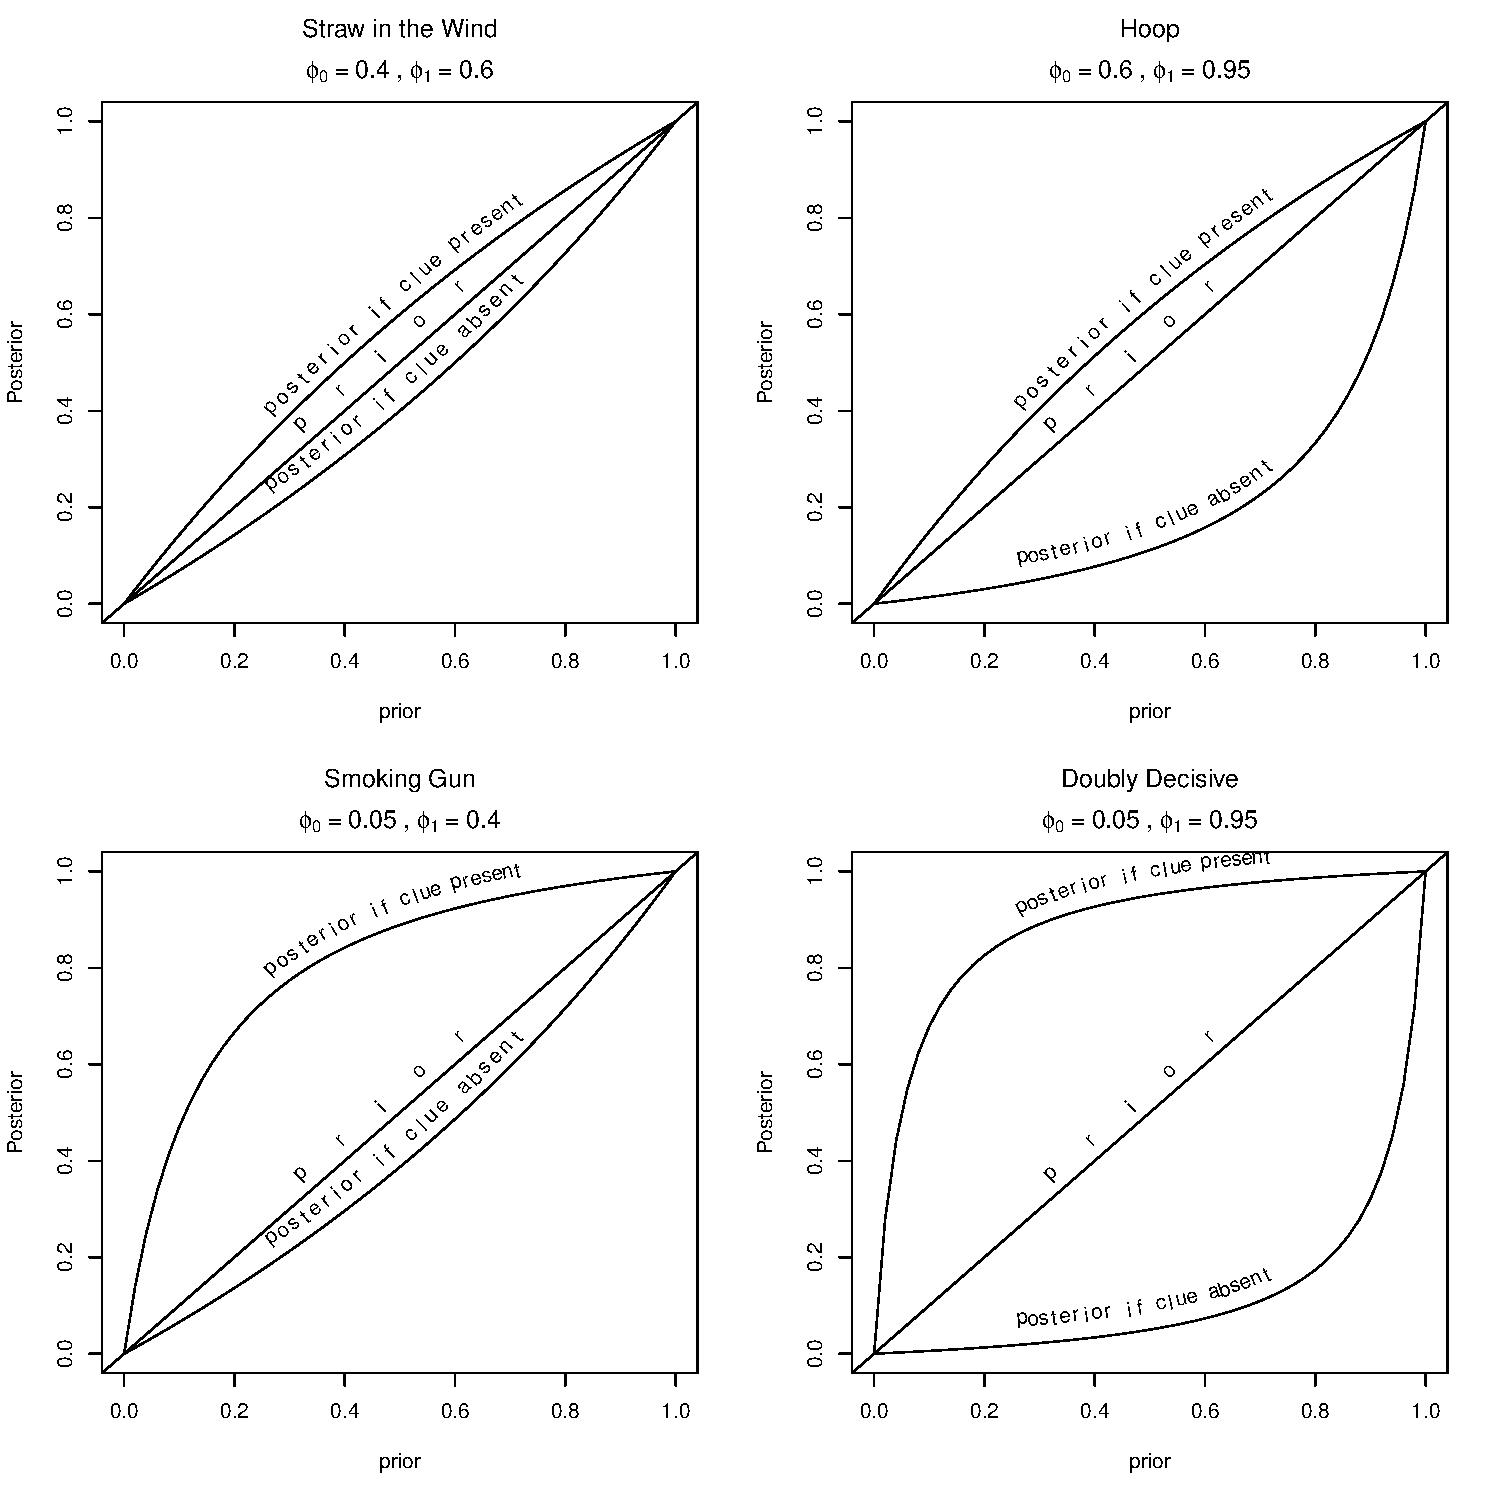
\includegraphics{ii_files/figure-latex/CluesInferences2-1} 

}

\caption{Figure shows how the learning from different types of tests depends on priors regarding the proposition. A smoking gun test has the greatest impact on beliefs when priors are middling low and the clue is observed; a ''hoop test'' has the greatest effect when priors are middling high and the clue is not observed.}\label{fig:CluesInferences2}
\end{figure}

The implication here is that our inferences with respect to a hypothesis must be based not just on the search for a clue predicted by the hypothesis but also on the \emph{plausibility} of the hypothesis, based on other things we know. Suppose, for instance, that we fail to observe evidence that we are 90 percent sure we \emph{should} observe if a hypothesized causal effect has occurred: a strong hoop test is failed. But suppose that the existing literature has given us a very high level of confidence that the hypothesis \emph{is} right. This high prior confidence, sometimes referred to as a ``base rate,'' is equivalent to believing that the causal effect exists in a very high proportion of cases. Thus, while any given case with a causal effect has only a 0.1 chance of not generating the clue, the high base rate means that the vast majority of cases that we observe without the clue will nonetheless be cases with causal effects. Thus, the failure of even a strong hoop test, involving a highly certain prediction, should only marginally reduce our confidence in a hypothesis that we strongly expect to be true.

A similar line of reasoning applies to smoking gun tests involving hypotheses that prior evidence suggests are very unlikely to be true. Innocent people may be very unlikely to be seen holding smoking guns after a murder. But if a very high proportion of people observed are known to be innocent, then a very high proportion of those holding smoking guns will in fact be innocent---and a smoking-gun clue will be far from decisive.

We emphasize two respects in which these implications depart from common intuitions. First, we cannot make \emph{general} statements about how decisive different categories of test, in Van Evera's framework, will be. It is commonly stated that hoop tests are devastating to a theory when they are failed, while smoking gun tests provide powerful evidence in favor of a hypothesis. But, in fact the amount learned depends not just on features of the clues but also on prior beliefs.

Second, although scholars frequently treat evidence that goes against the grain of the existing literature as especially enlightening, in the Bayesian framework the contribution of such evidence may sometimes be modest, precisely because received wisdom carries weight. Thus, although the discovery of \emph{disconfirming} evidence---an observation thought to be strongly inconsistent with the hypothesis---for a hypothesis commonly believed to be true is more informative (has a larger impact on beliefs) than \emph{confirming} evidence, this does not mean that we learn more than we would have if the prior were weaker. But it is not true as a general proposition that we learn more the bigger the ``surprise'' a piece of evidence is. The effect of disconfirming evidence on a hypothesis about which we are highly confident will be \emph{smaller} than it would be for a hypothesis about which we are only somewhat confident. When it comes to very strong hypotheses, the ``discovery'' of disconfirming evidence is very likely to be a false negative; likewise, the discovery of supporting evidence for a very implausible hypothesis is very likely to be a false positive. The Bayesian approach takes account of these features naturally.\footnote{We note, however, that one common intuition---that little is learned from disconfirming evidence on a low-plausibility hypothesis or from confirming evidence on a high-plausibility one---\emph{is} correct.}

\hypertarget{simultaneous-joint-updating}{%
\subsection{Simultaneous, joint updating}\label{simultaneous-joint-updating}}

When we update we often update over multiple quantities. When we see a smoking gun, for instance, we might update our beliefs that the butler did it, but we might also update our beliefs about how likely we are to see smoking guns---maybe they are not as rare as we thought!

Intuitively we might think of this updating as happening sequentially---first of all, we update over the general proposition, then we update over the particular claim. But in fact we update over both quantities at once.

Here we elaborate on the intuition using an example of Bayesian process tracing, in which updating occurs over both the nodal type (\(j\)) and beliefs about the probabilities with which clues are observed for each type (\(\phi\) values).

Suppose that we observe a case with values \(X=1, Y=1\). We begin by defining a prior probability distribution over each parameter. Suppose that we establish a prior categorical distribution reflecting uncertainty over whether the case is a \(b\) type (e.g., setting a probability of 0.5 that it is a \(b\) and 0.5 that is a \(d\) type). We also start with priors on \(\phi_b\) and \(\phi_d\). For concreteness, suppose that we are certain that the clue is unlikely for a \(d\) type (\(\phi_d=.1\)), but we are very uncertain about \(\phi_b\); in particular, we have a uniform prior distribution over \([0,1]\) for \(\phi_b\). Note that, even though we are very uncertain about \(\phi_b\), the clue still has probative value, arising from the fact that the expected value of \(\phi_b\) is higher than that of \(\phi_d\).

Suppose that we then look for the clue in the case and observe it. This observation shifts posterior weight away from a belief that the case is a \(d\). See Figure \ref{fig:correlation} for an illustration. Yet it \emph{simultaneously} shifts weight toward a higher value for \(\phi_b\) and a lower value for \(\phi_d\). The reason is that the observed clue has a relatively high likelihood \emph{both} for combinations of parameter values in which the case is a \(d\) and \(\phi_b\) is low \emph{and} for combinations in which the case is a \(b\) and \(\phi_b\) is \emph{high} (or, equivalently, in this example, where \(\phi_d\) is low). The marginal posterior distribution of \(\phi_b\) will thus be shifted upward relative to its prior marginal distribution. The joint posterior distribution will also reflect a dependency between the probability that the case is a \(b\) vs.~a \(d\), on the one hand, and \(\phi_b\) and \(\phi_d\) on the other.

\begin{figure}

{\centering 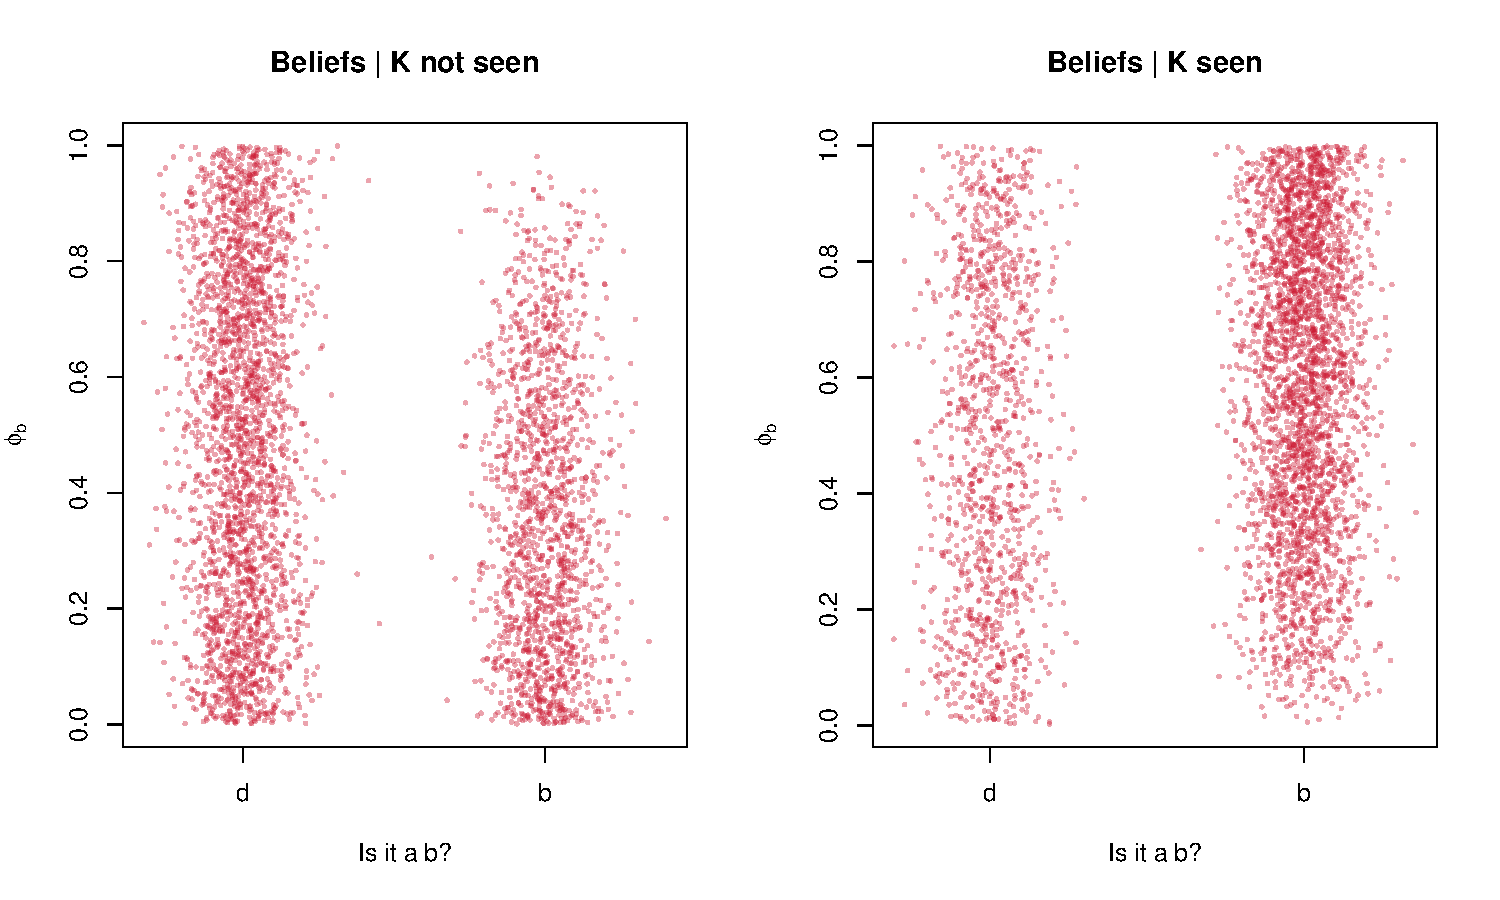
\includegraphics{ii_files/figure-latex/correlation-1} 

}

\caption{Joint posteriors distribution on whether a case is a $b$ or $d$ and on the probability of seeing a clue for a $b$ type ($\phi_b$).}\label{fig:correlation}
\end{figure}

Figure \ref{fig:ch5joint} provides a second example, this time showing the joint distribution for the belief that \(X\) causes \(Y\) in cases in which \(X=1, Y=1\) and the relative likelihood that \(K=1\) when \(X\) causes \(Y\) (and \(X=1, Y=1\)) relative to the likelihood that \(K=1\) when \(X\) does not cause \(Y\) (and \(X=1, Y=1\)). In this case the joint posterior is derived from a model in which probative value of \(K\) is inferred from data, rather than assumed by researchers. We develop more models of this form in later chapters but for now highlight only that in simple setups the distribution of beliefs over queries and over the informativeness of clues are likely not independent of each other.

\begin{figure}

{\centering 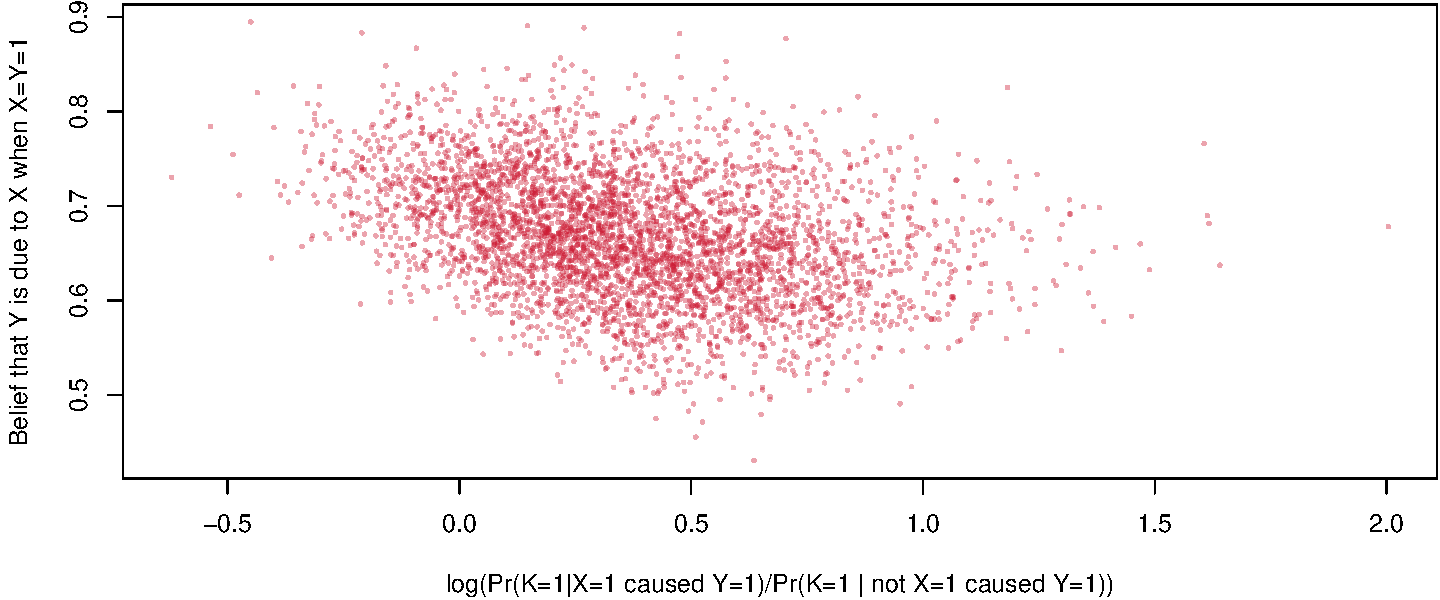
\includegraphics{ii_files/figure-latex/ch5joint-1} 

}

\caption{Correlated beliefs on queries and probative value}\label{fig:ch5joint}
\end{figure}

\hypertarget{posteriors-are-independent-of-the-ordering-of-data}{%
\subsection{Posteriors are independent of the ordering of data}\label{posteriors-are-independent-of-the-ordering-of-data}}

We often think of learning as a process in which we start off with some set of beliefs---our priors---we gather data, \(D_1\), and update our beliefs, forming a posterior; we then observe new data and we update again, forming a new posterior, having treated the previous posterior as a new prior. In such cases it might seem natural that it would matter which data we saw first and which later.

In fact, however, Bayesian updating is blind to ordering. If we learn first that a card is a face card and second that it is black, our posteriors that the card is a Jack of Spades go from 1 in 52 to 1 in 12 to 1 in 6. If we learn first that the card is black and second that it is a face card, our posteriors that it is a Jack of Spades go from 1 in 52 to 1 in 26 to 1 in 6. We end up in the same place in both cases. And we would have had the same conclusion if we learned in one go that the card is a black face card.

The math here is easy enough. Our posterior given two sets of data \(D_1, D_2\) can be written:

\[p(\theta | D_1, D_2) = \frac{p(\theta, D_1, D_2)}{p(D_1, D_2)} = \frac{p(\theta, D_1 | D_2)p(D_2)}{p(D_1 | D_2)p(D_2)}= \frac{p(\theta, D_1 | D_2)}{p(D_1 | D_2)}\]

or, equivalently:

\[p(\theta | D_1, D_2) = \frac{p(\theta, D_1, D_2)}{p(D_1, D_2)} = \frac{p(\theta, D_2 | D_1)p(D_1)}{p(D_2 | D_1)p(D_1)}= \frac{p(\theta, D_2 | D_1)}{p(D_2 | D_1)}\]

In other words our posteriors given both \(D_1\) and \(D_2\) can be thought of as the result of updating on \(D_2\) given we already know \(D_1\) or the result of updating on \(D_1\) given we already know \(D_2\).

This fact will be useful in applications. In practice we might assume that we have beliefs based on background data \(D_1\), for example regarding general relations between \(X\) and \(Y\) and a flat prior, and we then update again with new data on \(K\). Rather than updating twice, the fact that updating is invariant to order means that we can assume a flat prior and update once given data on \(X\), \(Y\), and \(K\).

\hypertarget{theory}{%
\chapter{Theories as causal models}\label{theory}}

\begin{headerbox}
We describe an approach in which theoretical claims are thought of as model justifications within a hierarchy of causal models. The approach has implications for consistency of inferences and for assessing when and how theory is useful.

\end{headerbox}

In Chapter \ref{illustratemodels}, we described a set of theories and represented them as causal models. But so far we haven't been very explicit in what we mean by a theory or how theory maps onto a causal-model framework.

In this book, we will think of theory as a type of \emph{explanation}: a theory provides an account of how or under what conditions a set of causal relationships operate. We generally express both a theory and the claims being theorized as causal models. The theory is then is a model that \emph{implies} another model---possibly with the help of some data.

To fix ideas: a simple claim might be that ``\emph{A} caused \emph{B} in case \(j\)''. This claim is itself a model, albeit a very simple one. The theory that supports this model might be of the form ``\emph{A} always causes \emph{B}'', ``\emph{A} always causes \emph{B} whenever \emph{C} (and \emph{C} holds in case \emph{j})'', or ``\emph{A} invariably causes \emph{B} and invariably \emph{B} causes \emph{C}''. These all have in common that they are arguments that could be provided to support the simple claim; in each case, if you believe the theory you believe the implication.

The rest of this short chapter builds out this idea and uses it to provide a way of characterizing when a theory is useful or not.
In the first section, we consider multiple senses in which one model might imply, and thus serve as a \emph{theory of}, another model. For one thing, we consider how one causal structure can imply (theorize) another causal structure, by including additional new nodes and nodal types that explain how or when causal effects in the original model will unfold. Next, we consider how the causal-type \emph{ranges} of models can relate to one another: one model can imply another model when the former's causal types constitute a subset of the latter's. In this situation, the theory represents a more specific, stronger claim about the kinds of causal effects that are operating. We then turn to logical relations between probabilistic models. We show how the distributions over nodal types in a simpler model structure can be underwritten by distributions over nodal types in a more detailed model structure. Here, a claim about the prevalence (or probability) of causal effects in a causal network is justified by claims about the prevalence or probability of causal effects in a more granular rendering of that network. Finally, we show how a probabilistic model plus \emph{data} can provide a theoretical underpinning for a new, stronger model.

Second, we consider how theories-as-models can be useful. In embedding theorization within the world of causal models, we ultimately have an empirical objective in mind. Theorizing a causal relationship of interest, in our framework, means elaborating our causal beliefs about the world in greater detail. As we show in later chapters, theorizing in the form of a causal model allows us to generate research designs: to identify sources of inferential leverage and to explicitly and systematically link observations of components of a causal system to the causal questions we seek to answer. In the second section of this chapter, however, we provide a high-level conceptualization of the empirical gains from theory.

In the chapter's third and final section, we show how our formalization of theory maps onto \emph{formal} theory as usually understood, showing how we can generate a causal model from a game-theoretic model.

\hypertarget{models-as-theories-of}{%
\section{\texorpdfstring{Models as \emph{theories of}}{Models as theories of}}\label{models-as-theories-of}}

Let us say that a causal model, \(M^\prime\), is a \emph{theory of} \(M\) if \(M\) is implied by \(M^\prime\). It is a theory \emph{because} it has implications. Otherwise it is a conclusion, an inference, or claim. A theory, \(M^\prime\), might itself sit atop---be supported by---another theory, \(M^{\prime\prime}\), that implies \(M^\prime\). To help fix the idea of theory as ``supporting'' or ``underlying'' the model(s) it theorizes, we refer to the theory, \(M^\prime\), as a \emph{lower}-level model relative to \(M\) and refer to \(M\) as a \emph{higher}-level model relative to its theorization, \(M^\prime\).\footnote{We note that our definition of theory differs somewhat from that given in \citet{pearl2009causality} (p207): there a theory is a (functional) causal model and a restriction over \(\times_j \mathcal{R}(U_j)\), that is, over the collection of contexts envisionable. Our definition also considers probabilistic models as theories, allowing statements such as ``the average effect of \(X\) on \(Y\) is 0.5.''}

Both structural models and probabilistic models---possibly in combination with data---imply other models. We discuss each in turn.

\hypertarget{implications-of-structural-causal-models}{%
\subsection{Implications of structural causal models}\label{implications-of-structural-causal-models}}

Structural models can imply multiple other simpler structural models. Similarly structural models can be implied by multiple more involved models.

We imagine two forms of lower level model, those that involve ``type splintering'' and those that involve ``type reduction.''

\textbf{Type splintering theorization.} Theorization often involves a refinement of causal types, implemented through the addition of nodes.
Take the very simple model, \(M\), represented in Figure \ref{fig:Highlow}(a). The model simply states that \(X\) has (or \emph{can} have) a causal effect on \(Y\).

What theories might justify \(M\)? This question can be rephrased as ``what models imply model \(M\)?'' The figure points to two possibilities. Both models \(M^\prime\) and \(M^{\prime\prime}\) imply model \(M\). They can be thought of as \emph{theories}, or lower-level model, of \(M\).

Model \(M^\prime\) differs by the addition of a node, \(K\), in the causal chain between \(X\) and \(Y\). We can say that \(M^\prime\) is a \emph{theory} of \(M\) for two reasons. First it provides a \emph{justification}---if you believe \(M^\prime\) you should believe \(M\): if \(X\) affects \(Y\) through \(K\), then \(X\) affects \(Y\). But as well as a justification it also provides an \emph{explanation} of \(M\). Suppose we already \emph{know} that \(X\) affects \(Y\) but want to know \emph{why}. If we ask, ``why does \(X\) affect \(Y\)?'', \(M^\prime\) provides an answer: \(X\) affects \(Y\) \emph{because} \(X\) affects \(K\), and \(K\) affects \(Y\).

Model \(M^{\prime\prime}\) differs by the addition of a node, \(C\), that moderates the effect of \(X\) on \(Y\). \(M^{\prime\prime}\) justifies \(M\) in the sense that if you believe \(M^{\prime\prime}\) you should believe \(M\). It provides an explanation of a kind also: if you believe model \(M^{\prime\prime}\) you likely believe that the relation between \(X\) and \(Y\) is what it is because of \(C\). Had \(C\) been different the causal relation between \(X\) and \(Y\) might have been also.

A key idea is that both \(M'\) and \(M''\) involve a redefinition of \(\theta^Y\). That is we see a change in the endogenous nodes but these in turn imply a change in the interpretation of the exogenous nodes pointing into existing endogenous nodes (such as \(Y\) in this example). We can think of part of \(\theta^Y\) being splintered off and captured by \(\theta^K\) or \(C\).

Return to models \(M\) and \(M'\) in Figure \ref{fig:Highlow}(a).
Importantly, in moving from the higher- to the lower-level model, we have effectively \emph{split} the nodal-type term \(\theta^Y\) into two parts: \(\theta^{Y_\text{lower}}\) and \(\theta^K\). Intuitively, in the higher-level model, (a), \(Y\) is a function of \(X\) and \(\theta^Y\), the latter representing all things other than \(X\) than can affect \(Y\). Or, in the language of our nodal-type setup, \(\theta^Y\) represents all of the (unspecified) sources of variation in \(X\)'s effect on \(Y\). When we insert \(K\) into the model, however, \(X\) now does not directly affect \(Y\) but only does so via \(K\). Further, we model \(X\) as acting on \(K\) in a manner conditioned by \(\theta^K\), which represents all of the (unspecified) factors determining \(X\)'s effect on \(K\). The key thing to notice here is that \(\theta^K\) now represents \emph{a portion of the variance that \(\theta^Y\) represented in the higher-level graph}: some of the variation in \(X\)'s effect on \(Y\) now arises from variation in \(X\)'s effect on \(K\), which is captured by \(\theta^K\). So, for instance, \(X\) might have no effect on \(Y\) because \(\theta^K\) takes on the value \(\theta^K_{00}\), so that \(X\) has no effect on \(K\). Put differently, any effect of \(X\) on \(Y\) must arise from an effect of \(X\) on \(K\); so \(\theta^K\)'s value must be either \(\theta^K_{01}\) or \(\theta^K_{10}\) for \(X\) to affect \(Y\). \footnote{As we emphasize further below, it is in fact only the random, unknown component of the \(X\rightarrow K\) link that makes the addition of \(K\) potentially informative as a matter of research design: if \(K\) were a deterministic function of \(X\) only, then knowledge of \(X\) would provide full knowledge of \(K\), and nothing could be learned from observing \(K\).} What \(\theta^K\) represents, then, is that part of the original \(\theta^Y\) that arose from some force other than \(X\) operating at the \emph{first} step of the causal chain from \(X\) to \(Y\).
So now, \(\theta^Y\) in the lower-level graph is not quite the same entity as it was in the higher-level graph. In the original graph, \(\theta^Y\) represented \emph{all} sources of variation in \(X\)'s effect on \(Y\). In the lower-level model, with \(K\) as mediator, \(\theta^Y\) represents only the variation in \(K\)'s effect on \(Y\). Put differently, \(\theta^Y\) has been expunged of any factors shaping the first stage of the causal process, which now reside in \(\theta^K\). We highlight this change in \(\theta^Y\)'s meaning by referring in the second model to \(\theta^{Y_\text{lower}}\).

Consider next model \(M^{\prime\prime}\) panel (c) in Figure \ref{fig:Highlow}, which also supports (implies) the higher-level model in panel \((a)\). The logical relationship between models \((a)\) and \((c)\), however, is somewhat different. Here the lower-level model \emph{specifies} one of the conditions that comprised \(\theta^Y\) in the higher-level model. In specifying a moderator, \(C\), we have extracted \(C\) from \(\theta^Y\), leaving \(\theta^{Y_\text{lower}}\) to represent all factors \emph{other than \(C\)} that condition \(Y\)'s response to its parents. More precisely, \(\theta^{Y_\text{lower}}\) now represents the set of nodal types defining how \(Y\) responds jointly to \(X\) and \(C\). Again, the relabeling as \(\theta^{Y_\text{lower}}\) reflects this change in the term's meaning. Whereas in Model \(M^{\prime}\) we have extracted \(\theta^K\) from \(\theta^Y\), in Model \(M^{\prime\prime}\), it is \(C\) itself that we have extracted from \(\theta^Y\), substantively specifying what had been just a random disturbance.

\begin{figure}

{\centering 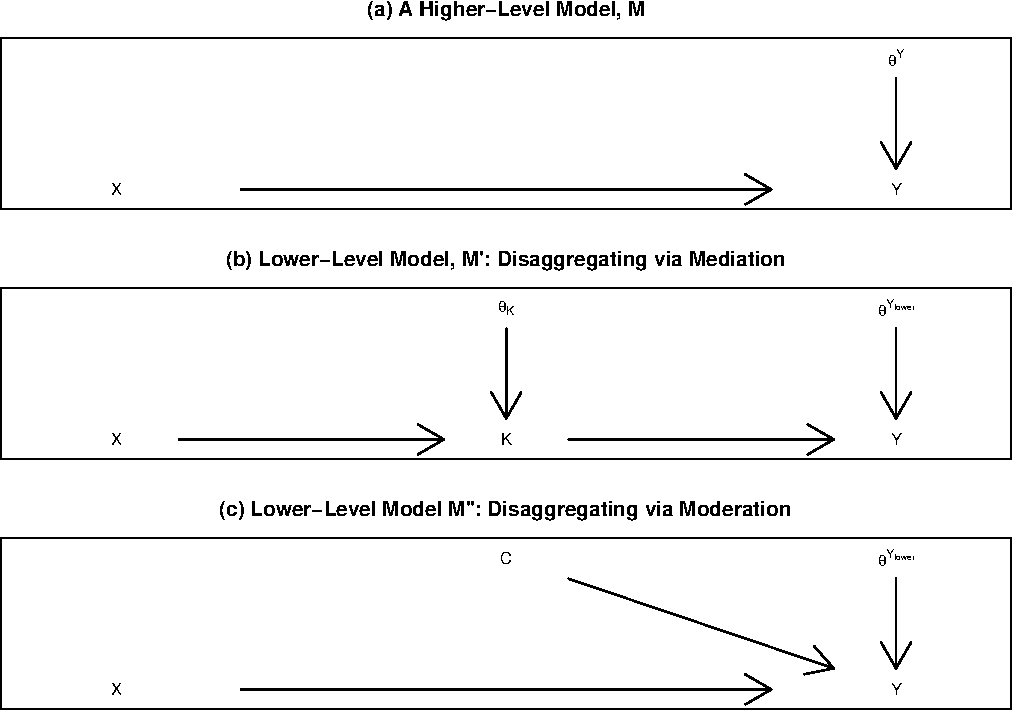
\includegraphics[width=0.8\linewidth]{ii_files/figure-latex/Highlow-1} 

}

\caption{Here we represent the simple claim that one variable causes another, and two theories --- lower-level models --- that could explain this claim. Both model (b) and model (c) involve theorization via disaggregation of nodes.}\label{fig:Highlow}
\end{figure}

\textbf{Type-reducing theorization.} There is a second way in which we might imagine a model being implied by another model that does not involve a change in nodes. Let \(\Theta(\mathcal M_1)\) denote the set of causal types in model \(\mathcal M_1\). Then we can say that \(\mathcal M_0\) implies \(\mathcal M_1\) if \(\Theta(\mathcal M_0)\subseteq \Theta(\mathcal M_1)\). Informally this means that any relation admitted by theory \(\mathcal M_0\) is representable in model \(\mathcal M_1\), though the converse may not be true. We can think of a theory of \(\mathcal M_1\) as a \emph{restriction} of ranges of \(\Theta(M_1)\).

We illustrate the idea in Figure \ref{fig:Highlowreduce}. In panel (a) of the figure, we have a model, \(\mathcal M_1\) in which \(Z\) can have both a direct and an indirect effect (via \(X\)) on \(Y\). Suppose that we believed that \(\mathcal M_1\) was technically true but overly permissive, in the sense that it allowed for causal relations that we do not in fact believe are operating. We might believe, for instance, that \(Z\) has no direct effect on \(Y\) and that \(Z\) has no negative effects on \(X\) --- the beliefs we would need to hold to treat \(Z\) as an instrument for \(X\). We could thus write down a lower-level model, \(\mathcal M_0\),in which we have \emph{reduced} the type space accordingly. Specifically, in \(\mathcal M_0\), we would restrict the nodal types at \(Y\) to only the \(\theta^Y_{0000}\), \(\theta^Y_{1100}\), \(\theta^Y_{0011}\), and \(\theta^Y_{1111}\); and we would reduce the nodal types at \(X\) to \(\theta^X_{00}\), \(\theta^X_{01}\), and \(\theta^X_{11}\). In panel (b), we (somewhat loosely) represent \(\mathcal M_0\). We have now eliminated the arrow from \(Z\) to \(Y\) to represent the dropping of all nodal types involving a direct effect of \(Z\) on \(Y\); not pictured is the montonicity assumption at \(X\). However, we have relabeled the nodal-type nodes for both \(X\) and \(Y\) to represent the fact that these are different objects from the nodal type nodes in the higher-level model.\footnote{We drop the arrow in Figure \ref{fig:Highlowreduce}, however, in order to help visually convey the difference between the two models. In fact, we would construct \(\mathcal M_0\) by placing restrictions at nodes in \(\mathcal M_1\), rather than by changing the model's structure, so that the allowed types in \(\mathcal M_0\) form a subset of those in \(\mathcal M_1\).}

Thus, while we can theorize by adding substantive nodes to a model and thus splitting types, we can also theorize by maintaining existing nodes but constraining relations among them. In both forms of theorization, we start with a model that allows for a broad, and possibly unknown, range of possibilities: for instance, a broad range of paths through which or conditions under which \(X\) might affect \(Y\) or a broad range of causal effects operating at each node. Theorization of both forms then involves making a \emph{stronger} claim: for instance, a claim about \emph{how} or \emph{when} \(X\) affects \(Y\) (via type-splintering) or a claim about the \emph{particular} causal effects operating at a given node (via type-reduction). In both forms of theory, believing the stronger claim in the lower-level model implies believing the weaker claim in the higher-level model. Further, both modes of theorization also map nicely onto common ways in which we think about theory-development in the social sciences: we theorize mechanisms, sources of heterogeneity, and directions of effects (starting with a belief that \(X\) affects \(Y\), for instance, and moving to a more constrained belief about whether that effect is positive or negative).

Finally, as we speak to below, theorization of both forms can generate gains for causal inference, by allowing us to use data in ways that we are unable to use it in the higher-level model.

\textbf{Preserving (conditional) independencies}

Not all potential mappings from higher- to lower-levels are permitted. In particular, when theorizing, we may \emph{add} but may not \emph{remove} independencies implied by the original model. If two variables are independent--- or conditionally independent given a third variable---in one model, then this same relation of independence (or conditional independence) must be captured in any theory of that model. For instance, if we start with a model of the form \(X \rightarrow Y \leftarrow W\), where \(W\) and \(X\) are independent, we could not theorize this model by adding an arrow from \(X\) to \(W\). A theory can have \emph{additional} conditional independencies not present in the higher-level model, as in the example in Figure \ref{fig:Highlowreduce}. But we may not theorize \emph{away} (conditional) independencies insisted on by our higher-level claim.

This is a key part of what it means for the lower-level model to \emph{justify} the higher-level model. A model makes claims about what is (conditionally) independent of what. The claims about conditional independence implied by the higher-level model must therefore be warranted by (conditional) independencies operating in the lower-level model. If we introduce new dependencies via theorization, then our higher-level model (which excludes these dependencies) would no longer be justified by the lower-level model.

\begin{figure}

{\centering 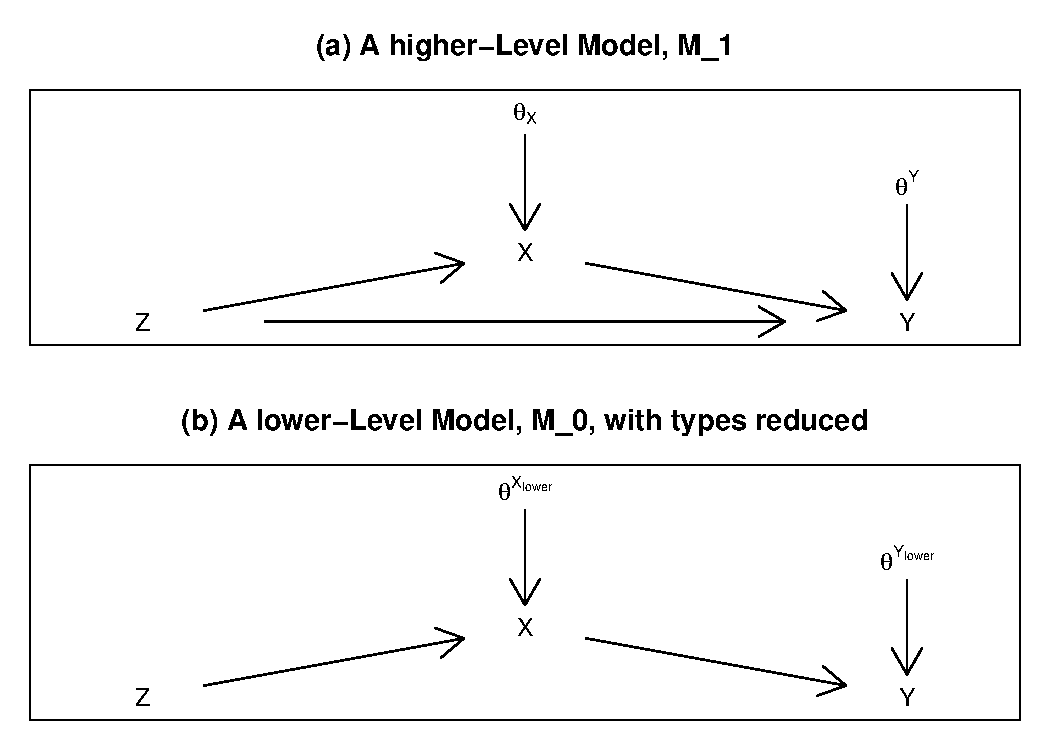
\includegraphics[width=0.8\linewidth]{ii_files/figure-latex/Highlowreduce-1} 

}

\caption{Here we represent theorization via type-reduction. Though we show the removal of an arrow to help convey the idea, we would in fact reduce types by imposing restrictions on the nodal types at Y within the same DAG.}\label{fig:Highlowreduce}
\end{figure}

\hypertarget{probabilistic-causal-models}{%
\subsection{Probabilistic causal models}\label{probabilistic-causal-models}}

At the structural level, then, there are two types of theory, or two types of relations between levels of model: those defined by type-splintering and those defined by type-reduction. In general, we will want to be working with probabilistic causal models --- i.e., those that include distributions over nodal types. We can describe straightforwardly how distributions in a higher-level model relate to --- and must change with --- distributions at the lower level. Indeed, it is these relations that unlock the opportunity for reaping empirical gains from theory.

\textbf{Theoretical implications of probabilistic models.} Suppose we start with the mediation model in panel (b) of Figure \ref{fig:Highlow}. Wen then add to it a distribution over \(\theta^K\) and \(\theta^Y_{lower}\), giving us a probabilistic causal model that we will denote \(\mathcal M^p_{lower}\). \(\mathcal M^p_{lower}\), in turn, implies a higher-level probabilistic model, \(\mathcal M^p_{higher}\), formed from the structure of Model (a) in Figure \ref{fig:Highlow}, and a \emph{particular} distribution over \(\theta^Y\): specifically, \(\theta^Y\) will have the distribution that preserves the causal relations implied by the beliefs in \(\mathcal M^p_{lower}\). Thus, for instance, the probability that \(X\) has a positive effect on \(Y\) in \(\mathcal M^p_{higher}\) is \(\theta^{Y}_{01}\); the probability that \(X\) has a positive effect on \(Y\) in \(\mathcal M^p_{lower}\) is \(\theta^{K_{lower}}_{01}\theta^{Y_{lower}}_{01} + \theta^{K_{lower}}_{10}\theta^{Y_{lower}}_{10}\). Consistency then requires that \(\theta^{M_{lower}}_{01}\theta^{Y_{lower}}_{01} + \theta^{K_{lower}}_{10}\theta^{Y_{lower}}_{10} = \theta^{Y_{higher}}_{01}\). So the value of \(\theta^{Y_{higher}}_{01}\) is \emph{implied} by \(\theta^{K_{lower}}_{01},\theta^{Y_{lower}}_{01}, \theta^{K_{lower}}_{10},\theta^{Y_{lower}}_{10}\), but not vice-versa.

\textbf{Deducing models from theory and data.} Now we can see what happens if we bring data to the lower-level model. A probabilistic causal model coupled with data implies another probabilistic causal model via Bayes rule. For this reason, we can fruitfully think of an initial model as being a \emph{theory of} an updated model, coupled with data. Thought of in this way we have clarity over what is meant when we turn to theory to support a claim, but also what is meant when we seek to justify a theory. We might imagine a scholar arguing: ``\(\mathcal M_1\): \(X\) caused \(Y\) in country \(j\).'' When pushed for a justification for the claim they provide the lower level model: ``\(\mathcal M_0:\) the average effect of \(X\) on \(Y\) in countries with feature \(C=1\) is 0.95, making it likely that \(X\) caused \(Y\) in this case.'' Here \(\mathcal M_1\) is implied by \(\mathcal M_0\) coupled with data \(C=1\). If pushed further as to why that theory is itself credible they might point to a lower level model consisting of structural model \(X\rightarrow Y \leftarrow C\) plus flat priors coupled with data on \(X,Y\) and \(C\). At each stage, as more justification is provided, the researcher formally provides lower-level models.

Moving up, as more data is provided, more ``specific'' higher level models emerge, justified by lower models plus data. These models are more specific in the sense that they are implied by the higher level models, plus data, but not vice versa. But they are also (generally) more specific in a second sense: that they make stronger statements about how causal processes operate.\footnote{This is not universally true, a point we return to below.} They place greater weight on a smaller set of causal claims.\footnote{In frequentist frameworks we often think of analysis as implementing up-or-down empirical tests against data to parse between theories that should be maintained and theories that should be rejected. In a Bayesian framework we think more continuously of shifting our beliefs across causal possibilities within a multi-dimensional theoretical space.}

As the simplest illustration, we might imagine beginning with an \(X\rightarrow Y\) model, \(\mathcal M_1\), in which, \(X\) and \(Y\) are binary, and we we believe that \(Y\) possibly responds to \(X\). If we have ``flat'' priors over causal types, in the sense described in Chapter \ref{bayeschapter}, then our prior uncertainty over the proposition that \(X\) causes \(Y\), under this model, is large; as is our uncertainty that \(Y=1\) is due to \(X=1\) in a given case. In other words, given our theory, we are uncertain about the proposition \(\mathcal M_3\): \(X\) caused \(Y\). However, if we then receive a lot of data, \(\mathcal D\), showing strong relations between \(X\) and \(Y\), then our updated model \(\mathcal M_2\), formed from combining \(\mathcal D\) and \(\mathcal M_1\) allows us to infer that \(X\) caused \(Y\) in this case with greater certainty.

Thus our new theory \(\mathcal M_2\) is (a) formally similar to \(\mathcal M_1\), (b) formed as a product of past theory plus evidence, here justified by \(\mathcal M_1\) given data \(\mathcal D\), and (c) capable of providing sharper implications than past theory.\footnote{As a general matter an updated theory may not provider sharper claims for all queries. That is, in practice, posterior variance over queries can increase with more data. As a simple illustration: say, we start out thinking that the probability that an outcome is due to conditions A, B, or C is .9, .05, and .05, respectively. If I find evidence that convinces me that A is not the cause, then I shift (a) to greater certainty about whether A was the cause but (b) greater uncertainty about whether B was the cause.}

In this way, Bayesian updating provides a simple and coherent way of thinking about the integration of theory and data.

\hypertarget{theorygains}{%
\section{Gains from theory}\label{theorygains}}

We now turn to consider how to think about whether a theory is \emph{useful}. We are comfortable with the idea that theories, or models more generally, are wrong. Models are not full and faithful reflections of reality; they are maps designed for a particular purpose. We make use of them because we think that they \emph{help} in some way.

But how do they actually help, and can we quantify the gains we get from using them?

We think we can. Using the notion of hierarchies of models, imagine we begin with model \(\mathcal M_1\), which together with data \(\mathcal D\), implies claim \(\mathcal M_2\). We then posit theory \(\mathcal M_0\) of \(\mathcal M_1\), so \(\mathcal M_0\) implies \(\mathcal M_1\). But when we bring \(\mathcal D\) to \(\mathcal M_0\) we get a new model, \(\mathcal M_2'\), that is different---and, hopefully, better---than \(\mathcal M_2\). Our gain from theory \(\mathcal M_0\) should be some summary of how much better \(\mathcal M_2'\) is than \(\mathcal M_2\).

Here is an illustration using a theory that allows use of the ``front-door criterion.''

Imagine that we have data on three variables, \(X\), \(Y\), and \(K\). We begin, however, with a model \(\mathcal M_1\) with confounding: \(C \rightarrow X \rightarrow Y \leftarrow C\). \(\mathcal M_1\) includes nodes for two of the three variables we have data on, \(X\) and \(Y\), but not \(K\). Assume, further, that we do not have data on node \(C\), the confound.

Suppose that we observe a strong correlation between \(X\) and \(Y\) and infer \(\mathcal M_2\): that \(X\) is a likely cause \(Y\). Our inference under \(\mathcal M_2\) is, however, quite uncertain because we are aware that the correlation may be due to the confound \(C\).

Suppose now that we posit the lower-level model \(\mathcal M_0\): \(C \rightarrow X \rightarrow K \rightarrow Y \leftarrow C\). \(\mathcal M_0\) now lets us make better use of data \(K\). If we observe, for instance, that \(X\) and \(K\) are uncorrelated, then we infer with confidence that in fact \(X\) did not cause \(Y\), despite the correlation.

Thus, in return for specifying a theory of \(\mathcal M_1\), we have been able to make better use of data and form a more confident conclusion. In this case, stating the theory, \(\mathcal M_0\), does not alter our \emph{priors} over our query. Our prior over the effect of \(X\) on \(Y\) may be identical under \(\mathcal M_1\) and \(\mathcal M_0\)---but our conclusions, given data, differ because the theory lets us make use of the data on \(K\), which we could not do under \(\mathcal M_1\) (which did not include \(K\)).

In other situations, we might imagine invoking a theory that does not necessarily involve new data but that allows us to make different, perhaps tighter inferences using the same data. An example might be the invocation of a type-reducing theory that involves a monotonicity restriction or exclusion restriction that allows for identification of a quantity that would not be identifiable without the theory.

Thus, one reason to theorize our models --- develop lower-level models that make stronger claims --- is to be able to reap greater inferential leverage from the more elaborate theory.

But are we, in fact, better off?

We might imagine answering the question in different ways: from an internal or external position, and from an \emph{ex ante} or \emph{ex post} perspective.

In all cases we ask how much better do we do as a result of making use of a theory.

If we are willing to posit an external ground truth, then we can define ``better'' in objective terms. An \emph{ex post}, objective way of operationalizing ``better'' is to assess the size of the error we make relative to the ground truth, from an inference that uses a theory, compared to an inference that does not make use of the theory. An objective \emph{ex ante} approach might be to ask what the expected error is from conclusions one draws given a theory. For instance: how wrong are we likely to be if we base our best guess on our posterior mean? ``How wrong'' might be operationalized in terms of mean squared error---the square of the distance between the truth and the posterior mean.\footnote{Other loss functions could be used, including functions that take account of the costs of collecting additional data or to the risks associated with false diagnoses. For instance, in \citet{heckerman1991toward}, an objective function is generated using expected utility gains from diagnoses generated based on new information over diagnoses based on what is believed already. In their treatment \citep[Equation 6]{heckerman1991toward}, the expected value of new information \(K\), given existing information \(W\) is: \(\sum{K}P(K|W)( EU(d(Q,W,K)|W, K) - EU(d(Q, W)|W, K))\) where \(EU\) is expected utility and \(d\) is the optimal inference (diagnosis) given available data. Note that the diagnosis can take account of \(K\) when it is observed, but the expected utility depends on \(K\) whether or not it is observed, as \(K\) carries information about the state of interest.}

A more subjective approach would be to ask about the reductions in posterior variance. \emph{Ex post} we can define ``better'' as the reduction in posterior variance from conclusions that make use of a theory compared to conclusions that do not. We might also think about the \emph{expected posterior variance}: how certain do you expect you will be after you make use of this new information?

More formally, imagine a situation in which there is an unknown parameter \(q\) and we have a data strategy that produces a distribution over data \(k\), given \(q\). Let \(p(q,k)\) denote the joint prior distribution over \(q\) and \(k\) with marginal distributions \(p(k)\) and \(p(q)\). For any \(k\) there is posterior estimate \(q_k\).

The squared error, given \(k\) is just \((q - q_k)^2\).

The \emph{expected} squared error is:

\[ESE := \int_q\int_k \left({q}_k-q\right)^2p(k, q)dkdq \]

This takes the error one might get with respect to any true value of the parameter (\(q\)), given the data one might see given \(q\) and the inferences one might draw.

For any \(k\) we might write the posterior variance as \(v_k\).

The \emph{expected} posterior variance can be written:

\[EV := \int_k v_k p(k)dk\]

This takes the posterior variance, given some data, over all the possible data one might see given marginal distribution \(p(k)\).

Interestingly, if we assess expectations using the same priors as you use for for forming posteriors the expected posterior variance and expected squared error are equivalent \citep{scharf1991statistical}.
To see this, we take advantage of the fact that \(p(q,k) = p(k)p(q|k) = p(q)p(k|q)\) and that \(p(q|k)\) gives the posterior distribution of \(q\) given \(k\). We then have:

\begin{align}
ESE &= \int_q\int_k \left({q}_k-q\right)^2p(q,k)dkdq \\
    &= \int_k\int_q \left({q}_k-q\right)^2p(k)p(q|k)dq dk \\
    &= \int_k\left[\int_q \left({q}_k-q\right)^2p(q|k)dq\right]p(k)dk \\
    &= \int_k v_k p(k)dk  = EV
\end{align}

Note that the key move is in recognizing that \(p(q |k)\) is in fact the posterior distribution on \(q\) given \(k\). In using this we assume that the same distribution is used for assessing error and for conducing analysis---that is we take the researcher's prior to be the relevant one for assessing error.

Moreover, it is easy to see that whenever inferences are sensitive to \(K\), the \emph{expected} variance of the posterior will be lower than the variance of the prior. This can be seen from the law of total variance, written here to highlight the gains from observation of \(K\), given what is already known from observation of \(W\).\footnote{See \citet{raiffa1961applied}. A similar expression can be given for the expected posterior variance from learning \(K\) in addition to \(W\) when \(W\) is not yet known. See, for example, Proposition 3 in \citet{geweke2014analysis}.}\\
\[Var(Q|W) = E_{K|W}(Var(Q|K,W)) +Var_{K|W}(E(Q|K,W))\]

However, although \emph{expected} posterior variance goes down, it is still always possible that posterior variance rises. The increase in uncertainty does not, however, mean you haven't been learning. Rather, you have learned that things aren't as simple as you thought.

One way to capture this idea that, although we are more uncertain, we think we are better off now than we were, is to ask: how much better are our guesses having observed \(K\) compared to what we would have guessed before, \emph{given} what we know having observed \(K\)? We will call this ``Wisdom'' to reflect the idea that it values appreciation of justifiable uncertainty:

\[Wisdom  = \int(q_0 - q)^2 - (q_k - q)^2 p(q | k)dq\]

This metric captures how much better off we are with the guess we have made given current data (\(q_k\)) compared to the guess we would have made if we had a theory that did not let us make use of it (\(q_0\)), knowing what we know having observe \(K\) (\(p(q|k)\).

An advantage of this conceptualization is that we can still record gains in learning even if the learning operates such that the posterior variance is larger than the prior variance. Even so, the implications for strategy are the same since wisdom is maximized by a strategy that reduces expected squared error.

Thus expected wisdom, is:

\begin{align}
\text{Expected Wisdom}  &= \int_q(q_0 - q)^2dq - \int_k\int_q(q_k - q)^2 p(q, k)dqdk \\
&= \text{Prior variance} - \text{Expected Posterior Variance}
\end{align}

We close with a reminder. Although expected reduction in variance and expected wisdom are both positive, both are are fundamentally subjective ideas, that presuppose the theory is correct. In contrast the expected error measure can be assessed under rival theoretical propositions and so allow for the real possibility that the gains of invoking a theory are negative.

\hypertarget{formal-theories-and-causal-models}{%
\section{Formal theories and causal models}\label{formal-theories-and-causal-models}}

It is relatively easy to see how the ideas above play out for what might be called empirical models. But in social sciences ``theory'' is a term sometimes reserved for what might be called analytic models. In this last section we work through how to use this framework when seeking to bring analytic models to data.

Let's start with analytic models. As an example we might consider the existence of ``Nash equilibria.'' Nash considered a class of settings (``normal form games'') in which each player \(i\) can choose an action \(\sigma_i\) from set \(\Sigma_i\) and receives a payoff \(u_i\) that depends on the actions of all players. A particular game, \(\Gamma\) is the collection of players, action sets, and payoffs.

Nash's theorem relates to the existence of a collection of strategies with the property that each strategy would produce the greatest utility for each player given the strategies of the other players. Such a collection of strategies is called a Nash equilibrium.

The claim that such a collection of strategies exists in these settings is an analytic claim. Unless there are errors in the derivation of the result, the claim is true in the sense that the conclusions follow from the assumptions. There is no evidence that we could go looking for in the world to assess the claim. The same can be said of the theoretical claims of many formal models in social sciences; they are theoretical conclusions of the if-then variety \citep{clarke2012model}.

We will refer to theories of this form as ``analytic theories.''

When researchers refer to a theory of populism or a theory of democratization however they generally do not have such pure theories in mind. Rather they have in mind what might be called ``applied theories'' (or perhaps more simply ``scientific theories'' or ``empirical theories''): general claims about the relations between objects in the world. The distinction here corresponds to the distinction in \citet{peressini1999applying} between ``pure mathematical theories'' and ``mathematized scientific theories.''\footnote{Or see the distinction, for instance in in Keynes, between pure theory and applied theory.}

Applied theory, in this sense, is a collection of claims with \emph{empirical} content: an applied theory refers to a set of propositions of causal relations in the world that might or might not hold, and is susceptible to assessment using data. These theories might look formally a lot \emph{like} analytic theories but it is better to think of them as translations at most. The relations between nodes of an applied theory are a matter of conjecture not a matter of necessity.\footnote{\citet{peressini1999applying} distinguishes between ``applied mathematical theories'' and ``mathematized scientific theories'' on the grounds that not all mathematized theories are an application of a pure theory.}

Though it is not standard practice, formal models produced by game theorists can often be translated and then represented using the notation of structural causal models in this way. Moreover, doing so may be fruitful. Using the approach described above we can then assess the utility of the applied theory, if not the pure theory itself.

For two players, for instance, we might imagine a representation of a game as shown in Figure \ref{fig:nfg}.

\begin{figure}

{\centering 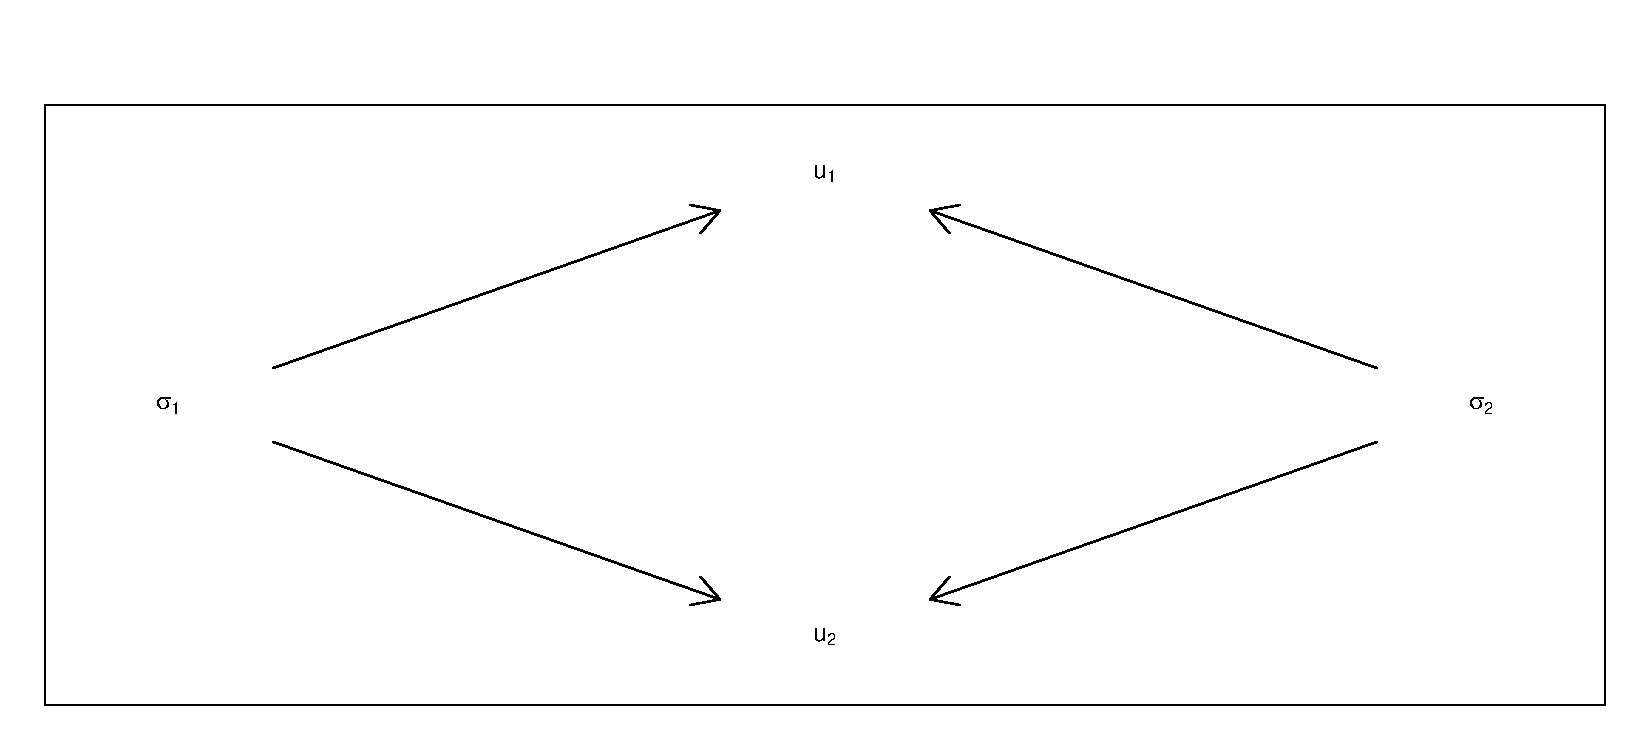
\includegraphics[width=0.8\linewidth]{ii_files/figure-latex/nfg-1} 

}

\caption{Formal structure of a normal form game.}\label{fig:nfg}
\end{figure}

Here the only functional equations are the utility functions. The utilities, given actions, are the implications of the theory, and so this is just a theory of how outcomes depend on social actions. It is not---yet---a behavioral theory.

In contrast to Nash's theorem regarding the existence of equilibria, a behavioral theory might claim that in problems that can be represented as normal form games, players indeed play Nash equilibrium. This is a theory about how people act in the world. We might call it Nash's theory.

How might this theory be represented as a causal model? Figure \ref{fig:nfg2} provides one representation.

\begin{figure}

{\centering 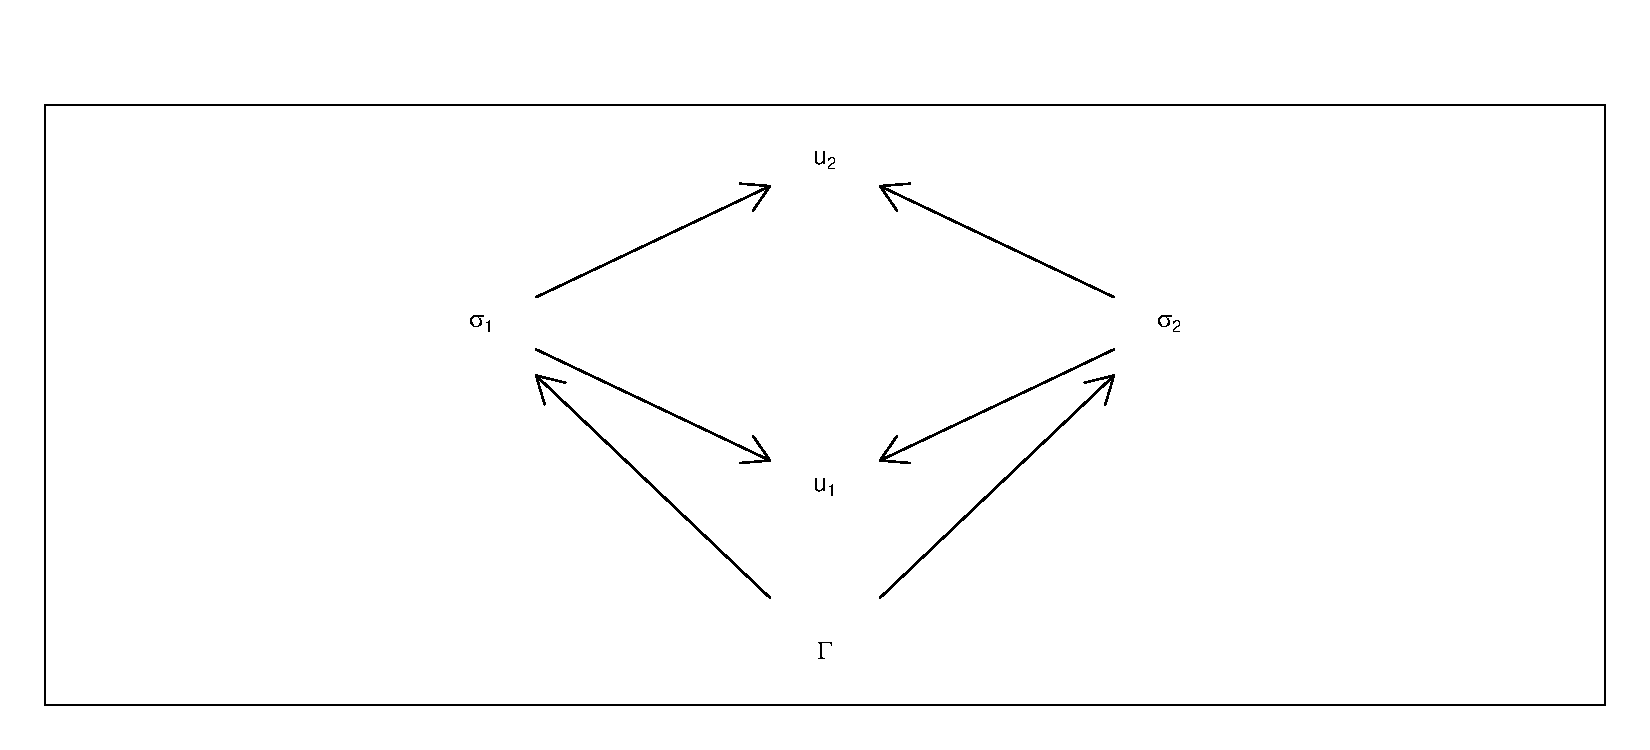
\includegraphics[width=0.8\linewidth]{ii_files/figure-latex/nfg2-1} 

}

\caption{Formal structure of a normal form game.}\label{fig:nfg2}
\end{figure}

Here beliefs about the game form (\(\Gamma\)) results in strategy choices by actors. If players play according to Nash's theory, \emph{the functional equations for the strategy choices are given by the Nash equilibrium solution itself}, with a refinement in case of multiplicity.

This model represents what we expect to happen in a game under Nash's theory and we can indeed see if the relations between nodes in the world look like what we expect under the theory. But it does not provide much of an \emph{explanation} for behavior.

A lower level causal model might help. In Figure \ref{fig:nfg3}
the game form \(\Gamma\) determines the beliefs about what actions the other player would make (thus \(\sigma_2^e\) is 1's belief about 2's actions). The functional equations for \(\sigma_2^e\) and \(\sigma_1^e\) might, for instance, be the Nash equilibrium solution itself: that is, players expect other players to play according to the Nash equilibrium (or in the case of multiple, a particular equilibrium selected using some refinement). The beliefs in turn, together with the game form (which contains \(u1, u_2\)), are what cause the players to select a particular action. The functional equation for \(\sigma_1\) might thus be \(\sigma_1 = \arg \max_\sigma u_1(\sigma, \sigma_2^e)\).

\begin{figure}

{\centering 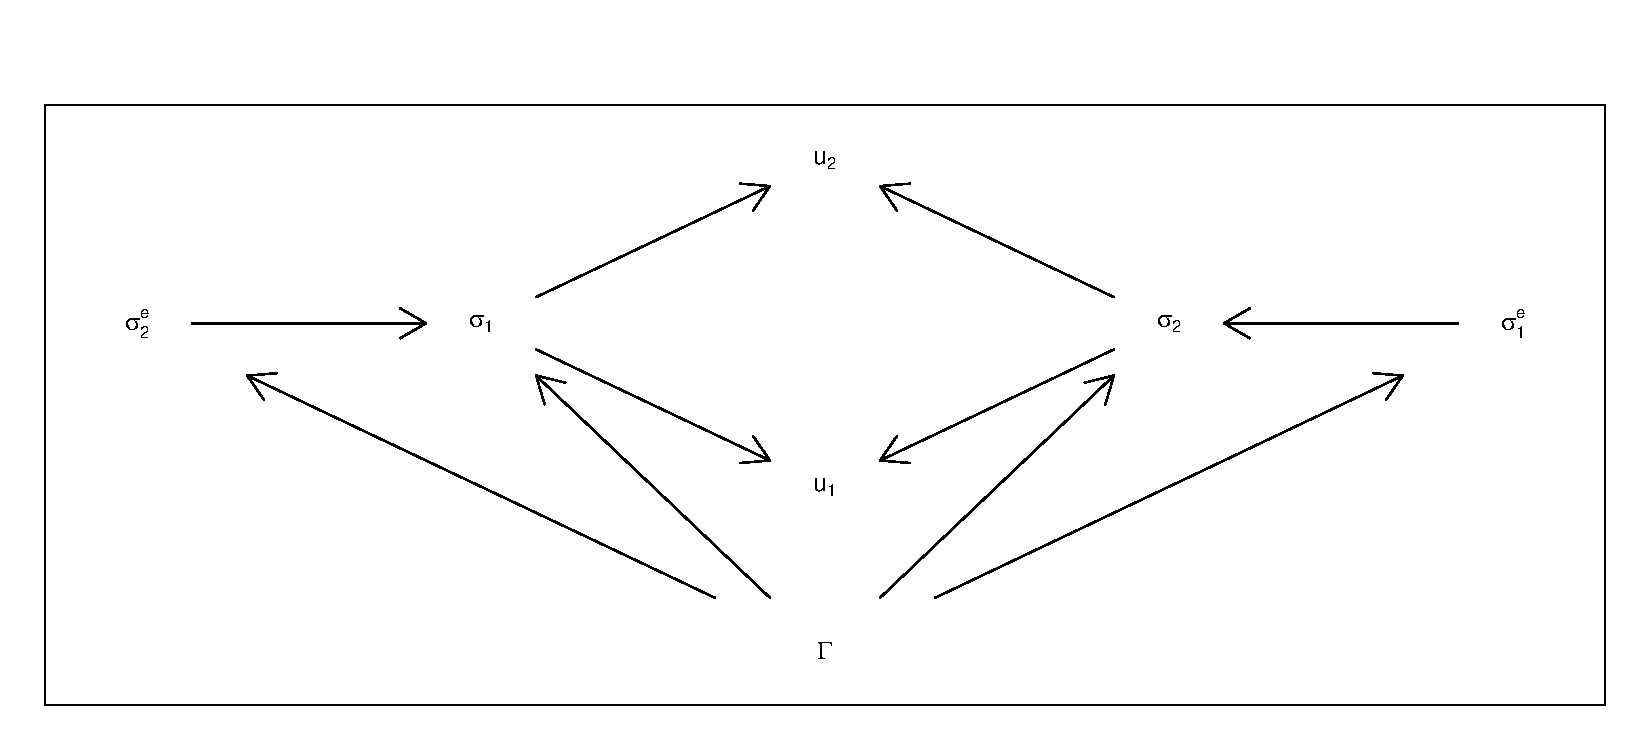
\includegraphics[width=0.8\linewidth]{ii_files/figure-latex/nfg3-1} 

}

\caption{Formal structure of a normal form game.}\label{fig:nfg3}
\end{figure}

This representation implies a set of relations that can be compared against empirical patterns. Do players indeed hold these beliefs when playing a given game? are actions indeed consistent with beliefs in ways specified by the theory. It provides a theory of beliefs and a theory of individual behavior as well as an explanation for social outcomes.

The model in Figure \ref{fig:nfg3} provides a foundation of sorts for Nash's theory. It suggests that players play Nash equilibria \emph{because} they expect others to and they are utility maximizers. But this is not the only explanation that can be provided; alternatively behavior might line up with the theory without passing through beliefs at all as suggested in some accounts from evolutionary game theory that show how processes might select for behavior that corresponds to Nash even if agents are unaware of the game they are playing.

One might step still further back and ask \emph{why} would actors form these beliefs, or take these actions, and answer in terms of assumptions about actor rationality. Figure \ref{fig:nfg4} for instance is a model in which actor rationality might vary and might influence beliefs about the actions of others as well as reactions to those beliefs. Fully specified functional equations might specify not only how actors act when rational but also how they react when they are not. In this sense the model in Figure \ref{fig:nfg4} both nests Nash's theory and provides an explanation for why actors conform to the predictions of the theory.

\begin{figure}

{\centering 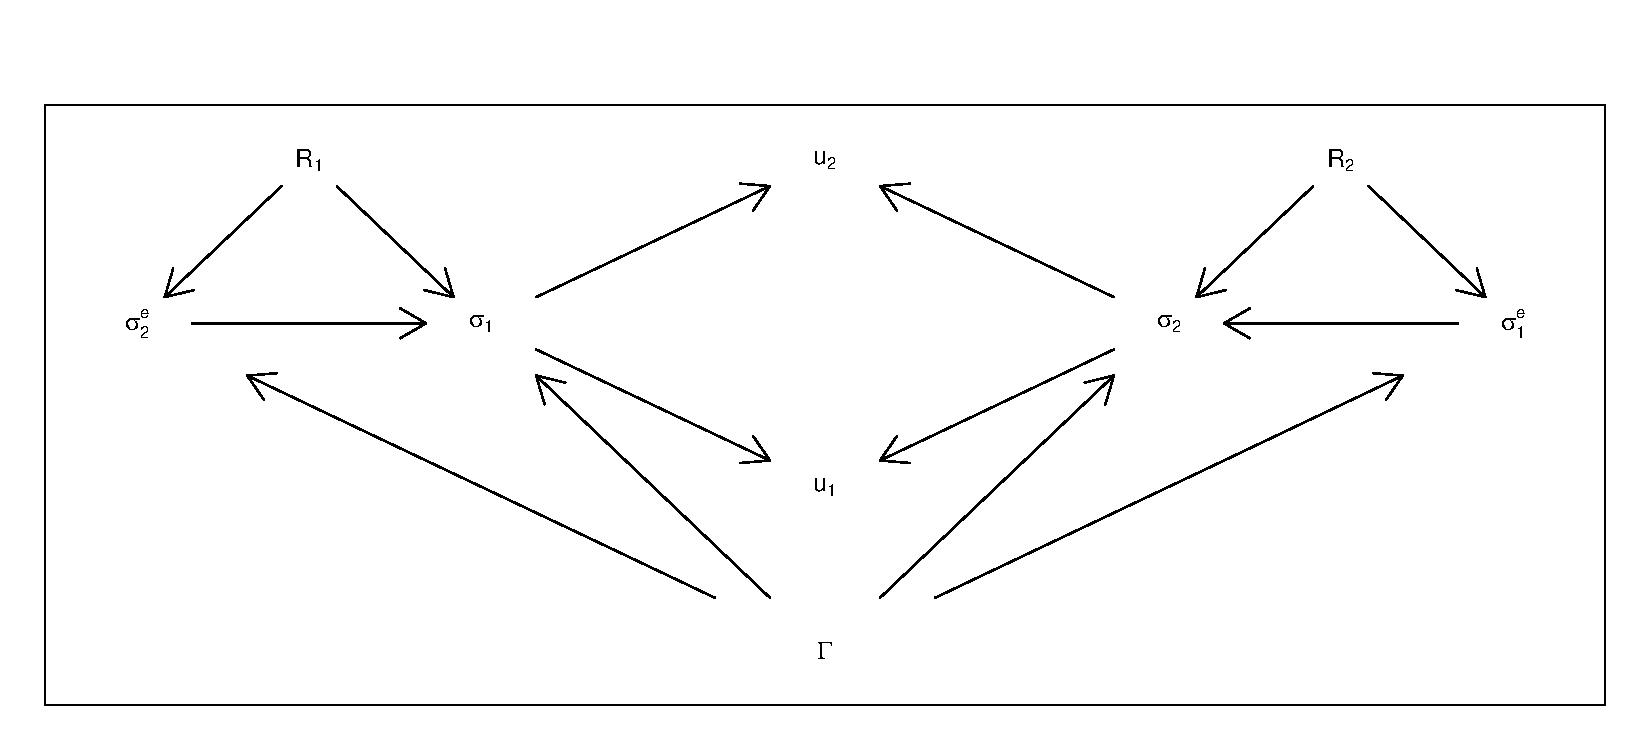
\includegraphics[width=0.8\linewidth]{ii_files/figure-latex/nfg4-1} 

}

\caption{Formal structure of a normal form game.}\label{fig:nfg4}
\end{figure}

In a final elaboration we can represent a kind of underspecification of Nash's theory that make it difficult to take the theory to data. In the above we assumed that players chose actions based on expectations that the other player would play the Nash equilibrium---or that the theory would specify which equilibrium in the case of multiplicity. But it is well known that Nash's theory often does not provide a unique solution. This indeterminacy can be captured in the Causal model as shown in Figure \ref{fig:nfg5} where a common shock---labelled \(\nu\), and interpreted as norms---interacts with the game form to determine the expectations of other players.

The functional equation for expectations can then allow for the possibility that (i) there is a unique equilibrium invariably chosen and played by both (ii) or a guarantee that players are playing one or other equilibrium together but uncertainty over which one is played, or (iii) the possibility that players are in fact out of sync, with each playing optimal strategies given beliefs but nevertheless not playing the same equilbria.

Nash's theory likely corresponds to position (ii). It can be captured by functional equations on beliefs given \(\nu\) but the theory does not specify \(\nu\), in the same way that it does not specify \(\Gamma\).

\begin{figure}

{\centering 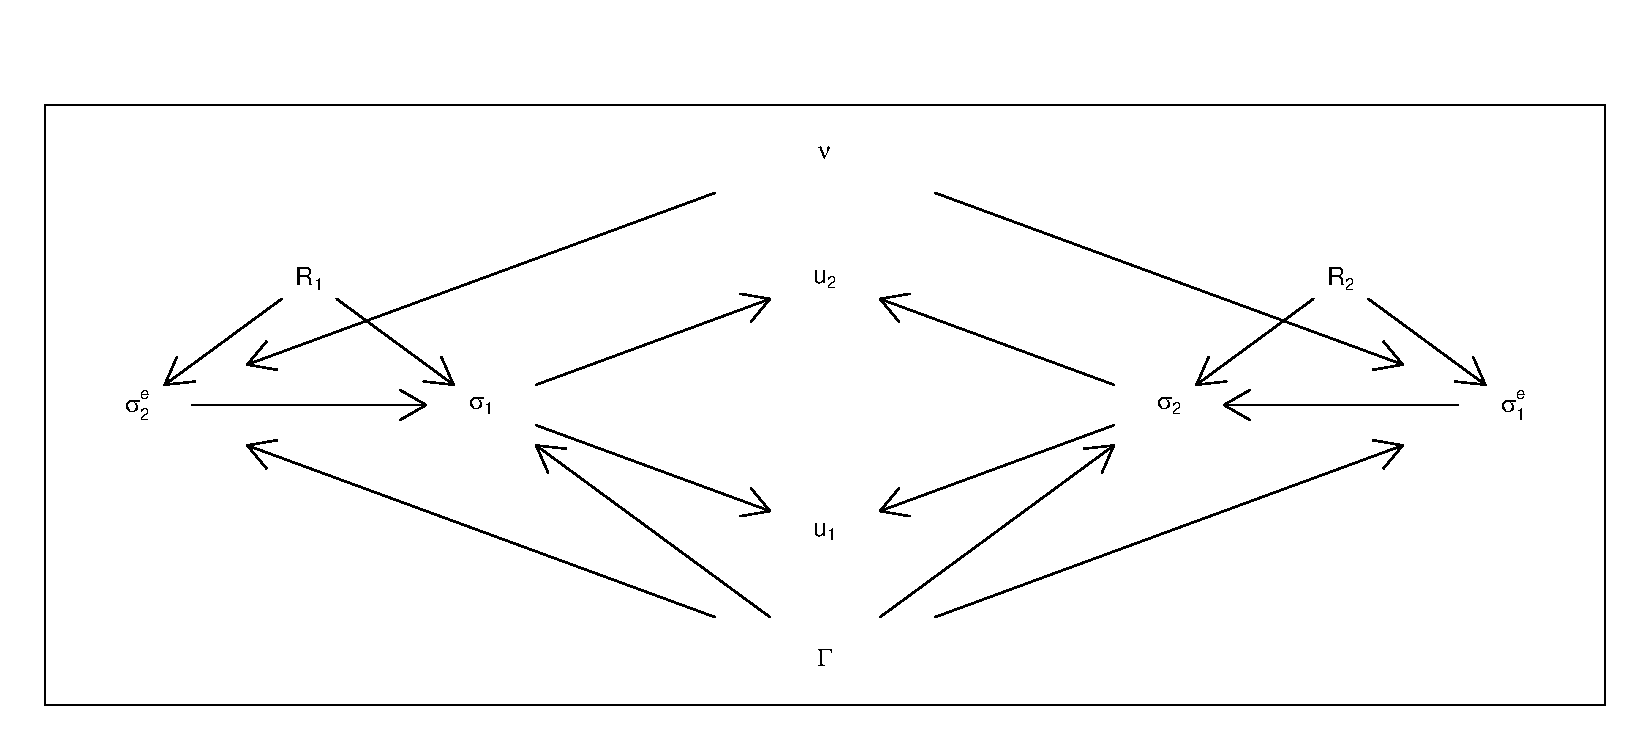
\includegraphics[width=0.8\linewidth]{ii_files/figure-latex/nfg5-1} 

}

\caption{A normal form game with a representation of equilibrium selection norms.}\label{fig:nfg5}
\end{figure}

We highlight three points from this discussion.

First the discussion highlights that thinking of theory as causal models does not force a sharp move away from abstract analytic theories; close analogues of these can often be incorporated in the same framework. This is true even for equilibrium analysis that seems to involve a kind of simultaneity on first blush.

Second, the discussion highlights how the causal modelling framework can make demands for specificity from formal theories. For instance specifying a functional relations from game form to actions requires a specification of a selection criterion in the event of multiple equilibria. Including agent rationality as a justification for the theory invites a specification for what would happen absent rationality.

Third the example shows a way of building a bridge from pure theory to empirical claims. One can think of Nash's theory as an entirely data free set of claims. When translated into an applied theory---a set of proposition about the ways actual players \emph{might} behave---and represented as a causal model, we are on a path to being able to use data to refine the theory. Thus we might begin with a formal specification like that in Figure \ref{fig:nfg5} but with initial uncertainty about player rationality, optimizing behavior, and equilibrium selection. This theory nests Nash but does not presume the theory to be a valid description of processes in the world. Combined with data, however, we shift to a more refined theory that selects Nash from the lower level model.

Finally, we can then apply the ideas of section \ref{theorygains} to applied formal theories and ask: is the theory useful? For instance, does data on player rationality help us better understand the relationship between game structure and welfare?

\hypertarget{pt}{%
\chapter{Process Tracing with Causal Models}\label{pt}}

\begin{headerbox}
We connect the literature on causal models to qualitative inference strategies used in process tracing and describe a procedure for inference on case level queries from causal models. We show how a key result from the causal models literature provides a condition for when clues may be (or certainly will not be) informative and extract a set of implications for process tracing.

\end{headerbox}

\hypertarget{process-tracing-and-causal-models}{%
\section{Process tracing and causal models}\label{process-tracing-and-causal-models}}

This chapter demonstrates how we can use causal models to conduct confirmatory process tracing: that is, to draw causal inferences about a single case from a causal model with data provided at the case-level.

\hypertarget{the-intuition}{%
\subsection{The intuition}\label{the-intuition}}

We first walk through the basic intuition and then provide a more formal account.

When we undertake process tracing, we seek to answer a causal question about a given case.
The key insight driving our approach is that the inference about a causal question for a case is a claim about \textbf{which causal types (collections of nodal types) are both likely ex ante (given prior knowledge) and consistent with the data}.\footnote{This differs from the task for mixed methods that we will address in Chapter \ref{mixing} as these concern claims about the distribution of causal types in populations.}

The question of interest can be about any number of case-level causal features, including questions about a case-level causal effect, the pathway through which an effect operates, an actual cause, or causal attribution. We use observations from the case itself to address this query. We do so via a procedure in which we first encode prior knowledge in the form of a causal model, then use data to learn about features of the model, and finally take what we have learned about the model and map it into our query.

Given a causal model, we form posteriors over queries as follows:

\begin{enumerate}
\def\labelenumi{\arabic{enumi}.}
\tightlist
\item
  \textbf{Specify all possible causal types for a model}. A causal type, recall, is a particular combination of nodal types for all nodes in a unit. That is, a single causal type specifies both a specific set of values of all exogenous variables in a model and the values that all endogenous variables \emph{would} potentially take on for all possible values of the exogenous variables. For a simple, binary \(X \rightarrow Y\) model, the number of possible causal types will be 2 (the number of possbile values \(X\), the exogenous node, can take on) times 4 (the number of possible nodal types for \(Y\), the endogenous node). Three of these causal types would be:
\end{enumerate}

\begin{itemize}
\tightlist
\item
  Type 1: (\(X=1\)) \emph{and} (\(Y=1\) if \(X=1\), \(Y=0\) if \(X=0\)).
\item
  Type 2: (\(X=0\)) \emph{and} (\(Y=1\) if \(X=1\), \(Y=0\) if \(X=0\)).
\item
  Type 3: (\(X=1\)) \emph{and} (\(Y=1\) if \(X=1\), \(Y=1\) if \(X=0\)).
\end{itemize}

Whatever the model, we generate a complete set of all possible causal types.

\begin{enumerate}
\def\labelenumi{\arabic{enumi}.}
\setcounter{enumi}{1}
\item
  \textbf{Specify priors over causal types.} We report how likely we think it is that a given unit is of a particular causal type. In the simplest situation, we might place 0 weight on some causal types (which might be ruled out by background theory, for example) and equal weight on the others.
\item
  \textbf{Specify the query in terms of causal types.} For instance, for the simple \(X \rightarrow Y\) model, the query ``\(Y\) responds positively to \(X\)'' can be thought of as a collection of causal types: Q=\{Type 1, Type 2\}.
\item
  \textbf{Once we observe the data, specify the set of causal types that are consistent with those data.} For instance, if we observe \(X=1, Y=1\) we might specify the data-consistent set as \{Type 1, Type 3\}, excluding Type 2 with which these data are inconsistent.
\item
  \textbf{Update.} Updating is then done by adding up the prior probabilities on all causal types that are consistent with both the data and the query, and dividing this sum by the sum of prior probabilities on all causal types that are consistent with the data (whether or not they are consistent with the query).
\end{enumerate}

\begin{figure}

{\centering 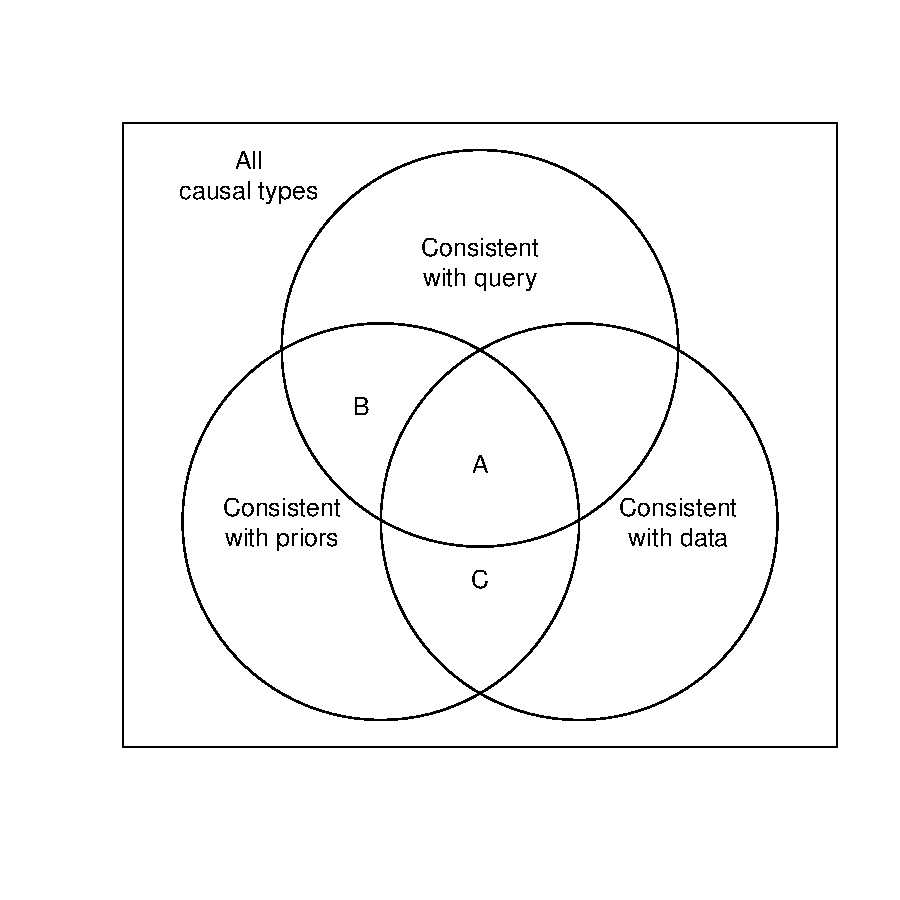
\includegraphics[width=0.5\linewidth]{ii_files/figure-latex/ptvenn-1} 

}

\caption{Logic of simple updating on arbitrary queries.}\label{fig:ptvenn}
\end{figure}

This process is represented graphically in Figure \ref{fig:ptvenn}, where we can think of probabilities as proportionate to areas. Our causal model defines the causal-type space. We then proceed by a process of elimination. Only some of the causal types in the model are consistent with prior knowledge. Only some are consistent with the data that we observe. Finally, any query itself maps onto a subset of the possible causal types. The causal types that remain in contention once we have observed the evidence are those at the intersection of consistency with priors and consistency with the data. \(A\) represents those types that are \emph{also} consistent with a given answer to the query (say, \(X\) has a positive effect on \(Y\)).

Thus, our belief about the query before we have seen the data is the probability of all causal types consistent with our priors and with the query (\(A + B\)) as a proportion of all types consistent with our priors. Once we have seen the data, we have reduced the permissible types to \(A + C\). Our posterior belief on the query is, then, the probabilities of those remaining types that are consistent with the query as a share of the probabilities of \emph{all} remaining types, or \(A/(A+C)\).

We now turn to a formalization of these ideas.

\hypertarget{a-formalization-of-the-general-approach}{%
\subsection{A formalization of the general approach}\label{a-formalization-of-the-general-approach}}

The general approach to inference draws on the components we outlined in chapters 2 to 4: graphical causal models (DAGs), queries, and priors. Coupled with data these elements provide grounds for causal inferences. We continue to focus on a situation with binary variables, though describe later how this can be extended. We walk through the procedure for simple models, though note that the approach outlined here can be applied to \emph{any} causal model with discrete variables and to any queries defined over the model.

The process tracing procedure operates as follows.

\hypertarget{the-model}{%
\subsubsection{The model}\label{the-model}}

First we need a model.

\textbf{A DAG}

We begin with a DAG, or graphical causal model. As discussed in Chapter \ref{models}, a DAG identifies a set of variables and describes the parent-child relations between them, indicating for each variable which other variables are its direct (possible) causes. These relationship, in turn, tell us which (non-descendant) variables a given variable is \emph{not} independent of given the other variables in the model.

\textbf{Nodal types}

Once we have specified a DAG, we can determine the full set of possible nodal types: the types defining the value that a variable will take on given the values of its parents, which we have denoted with \(\theta^j\) values for node \(j\), as in \(\theta^X_{0}\) or \(\theta^Y_{10}\). At each node, the range and number of possible nodal types is defined by the number of parents that that node has and the number of values the variables can take on. For instance, assuming all variables to be binary, if \(Y\) has parents \(X\) and \(W\), then there are \(2^{\left(2^2\right)}=16\) possible causal types for the \(Y\) node.

\textbf{Causal types}

From the set of all possible nodal types for a DAG, we get the set of all possible causal types by simply elaborating all possible permutations of nodal types.

\hypertarget{priors}{%
\subsection{Priors}\label{priors}}

Our background beliefs about a causal domain will usually consist of more than just beliefs about which variables have causal connections; they will also typically contain beliefs about what \emph{kinds} of effects operate between variables. That is, they will contain beliefs about which types are possible or, more generally, are more or less common in the world. We express these beliefs over causal effects as probability distributions over the nodal types. Beliefs about causal types are implied by beliefs about nodal types. In cases with unobserved confounding beliefs are defined over the joint distributions of nodal types.

For process tracing, our beliefs over nodal type \(\theta^j\), say, simply capture the subjective probability we have that the type takes on different values. We do not \emph{need} to defend this belief to use the machinery. We use \(\lambda^j_x\) to denote the probability that \(\theta^j = \theta^j_x\). Often however it helps with intuition to think of a given case of interest -- the one we are studying and seek to learn about -- as being drawn at random from a population and to think about our beliefs for the \emph{single} case as stemming from our beliefs about the population from which it is drawn. In that case \(\lambda^j_x\) can be thought of as a \emph{share}. So, for instance, our prior belief about the probability that inequality has a positive effect on democratization in Mexico in 1999 is our belief about how commonly inequality has a positive effect on democratization in the population of cases that are ``like'' Mexico in 1999.\footnote{The reference population for a case is defined based on whatever we already know about the case. Thus, for instance, if we already know that the case has \(Y=1\) before we begin process tracing, then the relevant population for the formation of prior beliefs is all cases in which \(Y=1\).}

A \(\lambda^j\) is simply a vector of numbers (or proportions), one for each possible nodal type, with all numbers non negative and summing to \(1\). So, for instance, \(\lambda^Y\) for our current example would be a vector with four values, each of which expresses a probability on one of the four nodal types at \(Y\). So we might have \(\lambda^Y_{01}=0.1\), \(\lambda^Y_{11}=0.05\), and so on -- with the \(\lambda^Y\) values summing to \(1\) because these values are defined over the full set of possible nodal types for \(Y\). For the purposes of this chapter we take \(\lambda\) as given---you start with beliefs; in later chapters however, when we move beyond single cases, \(\lambda\) becomes the quantity of interest.

Consider now beliefs over causal types. Let's start with with a situation in which we assume that the nodal types are independent of one another. We can think of this as a situation in which there is no confounding that is not captured in the graph -- no variable missing from the model that is a common ancestor of multiple nodes in the model. In this situation, our beliefs over causal types are simply the product of our beliefs over the component nodal types (since the joint probability of independent events is simply the product of their individual probabilities). For instance, one causal type might be ``a unit in which \(X=1\) and in which \(Y=1\) no matter what value \(X\) takes.'' In this case the probability that a case is of this causal type is \(\Pr(\theta^X = \theta^X_1)\Pr(\theta^Y = \theta^Y_{11}) = \lambda^X_1\lambda^Y_{11}\).

The simplest way in which we can express beliefs about the differential probabilities of different causal possibilities is by \emph{eliminating} nodal types that we do not believe to be possible---setting their parameter values to \(0\). Suppose, for instance, that we are examining the effect of ethnic diversity on civil war in a case. We might not know whether ethnic diversity causes civil war in this case, but we might have sufficient background knowledge to believe that ethnic diversity never has a \emph{negative} effect on civil war: it never prevents a civil war from happening that would have happened in the absence of ethnic diversity. We would thus want to set the parameter value for a negative causal effect to \(0\). If we then know nothing about the relative frequencies of the three remaining nodal types for \(Y\), we may (following the principle of indifference), frequency of positive effects, null effects with civil war destined to happen, and null effects with civil war never going to happen, assigning a weight of \(\frac{1}{3}\) to each of them.

In a situation of unobserved confounding, our beliefs over causal types are still well defined, though they are no longer the simple product of beliefs over nodal types. In this situation we need to describe a joint distribution over nodal types. In practice we can do this by specifying a probability for one nodal type and a conditional probability for another. Let us imagine for instance, in a simple \(X \rightarrow Y\) model, that we believe that some unobserved factor affects both the likelihood of \(X = 1\) and also \(X\)'s effect on \(Y\): maybe, for instance, \(X\) is more likely to be assigned to 1 where \(X\) has a positive effect. This is the same as saying that the probabilities of \(\theta^X\) and \(\theta^Y\) are correlated. Now, the probability of any combination of \(\theta^X\) and \(\theta^Y\) must be calculated using the joint probability formula, \(\Pr(A, B) = \Pr(A)\Pr(B|A)\).\footnote{In words, the probability of \(A\) and \(B\) occurring is equal to the probability of \(A\) occurring times the probability of \(B\) occurring \emph{given} that \(A\) occurs.} Thus, for instance, \(\Pr(\theta^Y = \theta^Y_{01}, \theta^X = \theta^X_1) = \Pr(\theta^Y = \theta^Y_{01})\Pr(\theta^X = \theta^X_1 | \theta^Y = \theta^Y_{01})\). To form priors over causal types in this situation, we need to posit beliefs about a set of more complex, conditional probabilities for \(X\)'s type. Specifically, we need to posit, \emph{for those cases} with a positive effect of \(X\) on \(Y\), what are the chances a case is ``assigned'' to \(X=1\); \emph{for those cases} with a negative effect, and similarly for other nodal types.

Thus for instance we represent \(\Pr(\theta^X_1, \theta^Y_{01}) = \Pr(\theta^X_1)\Pr(\theta^Y_{01}|\theta^X_1)\) which we write as \(\lambda^X_1, \lambda^{Y|\theta^X_1}_{01}\). The notation is awkward but the key thing is that we have a well defined set of beliefs that we need to take into account to assess the probability of different causal types.

In the \texttt{CausalQueries} package we represent the relationship parameters and causal types using a ``parameter matrix.'' This matrix has a row for each parameter, a column for each causal type, and cell entries that indicate whether the parameter forms part of the type probability. In models without confounding we have a parameter for each nodal type. In the \(X \rightarrow Y\) model, for instance, the causal causal type (\(\theta^X_1, \theta^Y_{10}\)), has a 1 in the \(\lambda^X_1\) row and a 1 in the \(\lambda^Y_{10}\) row only, indicating that the product of these probabilities gives the probability of the causal type. In models with confounding the logic is the same except that we have rows for as many conditional probabilities as we need to fully characterize joint distributions.

\hypertarget{possible-data-types.}{%
\subsubsection{Possible data types.}\label{possible-data-types.}}

A \emph{data type} is a particular pattern of data that we could potentially observe for a given case. More specifically, a data type is a set of values, one for each node in a model. For instance, in our \(X, W, Y\) setup, \(X=1, W=0, Y=0\) would be one data type.

Importantly, absent intervention, each possible causal type \emph{maps deterministically into a single data type.} One intuitive way to think about why this is the case is that a causal type tells us (a) the values to which all exogenous variables in a model are assigned and (b) how all endogenous variables respond to their parents. Given these two components, only one set of node values is possible. For example, causal type \(\theta = (\theta^X = \theta^X_1, \theta^W = \theta^W_0, \theta^Y = \theta^Y_{0100})\) imples data \(X=1, W=0, Y=1\). Absent intervention, there is no other set of data that can be generated by this causal type.

Equally importantly, however, \emph{the mapping from causal types to data types is not one-to-one.} More than one causal type can generate the same case-level data pattern. For instance, the causal type \(\theta = (\theta^X = \theta^X_1, \theta^W = \theta^W_0, \theta^Y = \theta^Y_{1101})\) will \emph{also} generate the data type, \(X=1, W=0, Y=1\). Thus, observing this data type leaves us with ambiguity about the causal type by which it was generated.

In the \texttt{CausalQueries} package we use an \emph{ambiguity matrix} to summarize the mapping between causal types and data types. There is a row for each causal type and a column for each data type and an entry of 1 indicates that the causal type generates the data type. Each row has a single 1 but each column can have many 1s---an indicator of the ambguity we have regarding causal types when we observe data types.

\begin{longtable}[]{@{}cccccc@{}}
\caption{\label{tab:ambigmatrix}. An ambiguity matrix, mapping from data types to causal types for a simple \(X \rightarrow Y\) model.}\tabularnewline
\toprule
\textbf{Data types} \(\rightarrow\) & X0Y0 & X1Y0 & X0Y1 & X1Y1 & Priors \\
\midrule
\endfirsthead
\toprule
\textbf{Data types} \(\rightarrow\) & X0Y0 & X1Y0 & X0Y1 & X1Y1 & Priors \\
\midrule
\endhead
\textbf{Causal types} \(\downarrow\) & & & & & \\
\(\theta^X_0,\theta^Y_{00}\) & 1 & 0 & 0 & 0 & 0.1 \\
\(\theta^X_1,\theta^Y_{00}\) & 0 & 1 & 0 & 0 & 0.1 \\
\(\theta^X_0,\theta^Y_{10}\) & 0 & 0 & 1 & 0 & 0.1 \\
\(\theta^X_1,\theta^Y_{10}\) & 0 & 1 & 0 & 0 & 0.1 \\
\(\theta^X_0,\theta^Y_{01}\) & 1 & 0 & 0 & 0 & 0.2 \\
\(\theta^X_1,\theta^Y_{01}\) & 0 & 0 & 0 & 1 & 0.2 \\
\(\theta^X_0,\theta^Y_{11}\) & 0 & 0 & 1 & 0 & 0.1 \\
\(\theta^X_1,\theta^Y_{11}\) & 0 & 0 & 0 & 1 & 0.1 \\
\bottomrule
\end{longtable}

As models get more complex, the numbers of causal and data types multiply, though generally the number of causal types increases faster than the number of data types. For a simple mediation model (\(X \rightarrow M \rightarrow Y\)) there are \(2^3 = 8\) data types---possible combinations of values for \(X,M,Y\) but \(2\times 4 \times 4\) causal types.

The ambiguities matrix tells us what types are data consistent and, in doing so, shapes our inferences.
Table \ref{tab:ambigmatrixmed} shows a portion of the ambiguities matrix for the \(X \rightarrow M \rightarrow Y\) model, with priors on causal types appended in the final column. In this model if we observe \(X=1, M=0, Y=0\) we have ambiguities over causal types. These data tell us that \(\theta^X = \theta^X_1\). But they do not tell us whether \(M\)'s type is such that \(X\) has a negative effect on \(M\) (\(\theta^M_{10}\)) or \(X\) has no effect with \(M\) fixed at \(0\) (\(\theta^M_{00}\)). Similarly, we do not know whether \(M\) has a positive effect on \(Y\) (\(\theta^Y_{01}\)) or no effect with \(Y\) fixed at \(0\) (\(\theta^Y_{00}\)). This leaves four combinations of nodal types---four causal types---that are consistent with the data. These types are picked out by the ambiguities matrix.

\begin{table}

\caption{\label{tab:ambigmatrixmed}Excerpt from the ambiguity matrix for a chain model. Rows are causal types, columns are data types. Last column shows possible priors over rows.}
\centering
\resizebox{\linewidth}{!}{
\begin{tabular}[t]{lrrrrrrr}
\toprule
  & X0M0Y0 & X1M0Y0 & X0M1Y0 & X1M1Y0 & X0M0Y1 & X1M0Y1 & prior\\
\midrule
\cellcolor{gray!6}{X0M00Y00} & \cellcolor{gray!6}{1} & \cellcolor{gray!6}{0} & \cellcolor{gray!6}{0} & \cellcolor{gray!6}{0} & \cellcolor{gray!6}{0} & \cellcolor{gray!6}{0} & \cellcolor{gray!6}{0.02}\\
X1M00Y00 & 0 & 1 & 0 & 0 & 0 & 0 & 0.02\\
\cellcolor{gray!6}{X0M10Y00} & \cellcolor{gray!6}{0} & \cellcolor{gray!6}{0} & \cellcolor{gray!6}{1} & \cellcolor{gray!6}{0} & \cellcolor{gray!6}{0} & \cellcolor{gray!6}{0} & \cellcolor{gray!6}{0.02}\\
X1M10Y00 & 0 & 1 & 0 & 0 & 0 & 0 & 0.02\\
\cellcolor{gray!6}{X0M01Y00} & \cellcolor{gray!6}{1} & \cellcolor{gray!6}{0} & \cellcolor{gray!6}{0} & \cellcolor{gray!6}{0} & \cellcolor{gray!6}{0} & \cellcolor{gray!6}{0} & \cellcolor{gray!6}{0.04}\\
\addlinespace
X1M01Y00 & 0 & 0 & 0 & 1 & 0 & 0 & 0.04\\
\cellcolor{gray!6}{X0M11Y00} & \cellcolor{gray!6}{0} & \cellcolor{gray!6}{0} & \cellcolor{gray!6}{1} & \cellcolor{gray!6}{0} & \cellcolor{gray!6}{0} & \cellcolor{gray!6}{0} & \cellcolor{gray!6}{0.02}\\
X1M11Y00 & 0 & 0 & 0 & 1 & 0 & 0 & 0.02\\
\cellcolor{gray!6}{X0M00Y10} & \cellcolor{gray!6}{0} & \cellcolor{gray!6}{0} & \cellcolor{gray!6}{0} & \cellcolor{gray!6}{0} & \cellcolor{gray!6}{1} & \cellcolor{gray!6}{0} & \cellcolor{gray!6}{0.02}\\
X1M00Y10 & 0 & 0 & 0 & 0 & 0 & 1 & 0.02\\
\addlinespace
\cellcolor{gray!6}{X0M10Y10} & \cellcolor{gray!6}{0} & \cellcolor{gray!6}{0} & \cellcolor{gray!6}{1} & \cellcolor{gray!6}{0} & \cellcolor{gray!6}{0} & \cellcolor{gray!6}{0} & \cellcolor{gray!6}{0.02}\\
X1M10Y10 & 0 & 0 & 0 & 0 & 0 & 1 & 0.02\\
\cellcolor{gray!6}{X0M01Y10} & \cellcolor{gray!6}{0} & \cellcolor{gray!6}{0} & \cellcolor{gray!6}{0} & \cellcolor{gray!6}{0} & \cellcolor{gray!6}{1} & \cellcolor{gray!6}{0} & \cellcolor{gray!6}{0.04}\\
X1M01Y10 & 0 & 0 & 0 & 1 & 0 & 0 & 0.04\\
\cellcolor{gray!6}{X0M11Y10} & \cellcolor{gray!6}{0} & \cellcolor{gray!6}{0} & \cellcolor{gray!6}{1} & \cellcolor{gray!6}{0} & \cellcolor{gray!6}{0} & \cellcolor{gray!6}{0} & \cellcolor{gray!6}{0.02}\\
\addlinespace
X1M11Y10 & 0 & 0 & 0 & 1 & 0 & 0 & 0.02\\
\bottomrule
\end{tabular}}
\end{table}

\hypertarget{updating-on-types-given-the-data.}{%
\subsection{Updating on types given the data.}\label{updating-on-types-given-the-data.}}

Once we observe actual data in a case, we can then update on the probabilities assigned to each causal type. The logic is simple. When we observe a set of data from a case, we place \(0\) probability on all causal types that could not have produced these data; we then scale up the probabilities on all causal types that could have.

As a simple example imagine we have an \(X\rightarrow Y\) model with equal prior weights (1/8) on each of the eight possible causal types. Now, suppose that we observe the data \(X=1, Y=1\), i.e., data type \(X1Y1\). This data is consistent with some causal types but not others. Only two causal types are consistent with the data: \(\theta^X_1, \theta^Y_{01}\) and \(\theta^X_1, \theta^Y_{11}\). We therefore put 0 weight on all other causal types and scale up the remaining probabilities so that they sum to 1 (preserving the ratio between them). The result gives \emph{posterior} probabilities on the causal types. We display an ``updated'' ambiguity matrix, with excluded data types and causal types removed, in Table \ref{tab:ambigupdate}.

Before we see any data on the case at hand, then, we believe (based on our beliefs about the population to which the case belongs) that there is a 1/8 probability that the case is one in which \(X\) is assigned to \(1\) and has a positive effect on \(Y\); and 1/8 probability that it's a case in which \(X\) gets assigned to \(1\) and has no effect on \(Y\) (and so \(Y\) is \(1\) regardless of \(X\)). Seeing the \(X=1, Y=1\) data, we now believe that there is a 1/2 probability that the case is of the former type, and a 1/2 probability that it is of the latter type. Had our prior beliefs on types been different from each other, the posterior beliefs would have scaled up accordingly.

\begin{longtable}[]{@{}cccc@{}}
\caption{\label{tab:ambigupdate}. Ambiguities in an \(X \rightarrow Y\) model after observing \(X=1, Y=1\) in a case.}\tabularnewline
\toprule
\textbf{Data types} \(\rightarrow\) & X1Y1 & Priors & Posteriors \\
\midrule
\endfirsthead
\toprule
\textbf{Data types} \(\rightarrow\) & X1Y1 & Priors & Posteriors \\
\midrule
\endhead
\textbf{Causal types} \(\downarrow\) & & & \\
\(\theta^X_1,\theta^Y_{01}\) & 1 & 1/8 & 1/2 \\
\(\theta^X_1,\theta^Y_{11}\) & 1 & 1/8 & 1/2 \\
\bottomrule
\end{longtable}

We now walk through how this work for the more complex \(X \rightarrow M \rightarrow Y\) model, and the ambiguity matrix in Table \ref{tab:ambigmatrixmed}. If we observe the data \(X=1, M=0, Y=0\), for instance, this exercise would yield the updated ambiguity matrix in Table \ref{tab:ambigmedupdate}. Here we have eliminated all rows (causal types) with a \(0\) in the relevant data-type column (\(X1M0Y0\)) and formed the posteriors by scaling up the priors in the retained rows.

\begin{longtable}[]{@{}cccc@{}}
\caption{\label{tab:ambigmedupdate}. An updated version of the ambiguity matrix in Table \ref{tab:ambigmatrixmed}, after observing \(X=1, M=0, Y=0\) in a case.}\tabularnewline
\toprule
\textbf{Data types} \(\rightarrow\) & X1M0Y0 & Priors & Posteriors \\
\midrule
\endfirsthead
\toprule
\textbf{Data types} \(\rightarrow\) & X1M0Y0 & Priors & Posteriors \\
\midrule
\endhead
\textbf{Causal types} \(\downarrow\) & & & \\
\(\theta^X_1,\theta^M_{00},\theta^Y_{00}\) & 1 & 0.02 & 0.1667 \\
\(\theta^X_1,\theta^M_{10},\theta^Y_{00}\) & 1 & 0.02 & 0.1667 \\
\(\theta^X_1,\theta^M_{00},\theta^Y_{01}\) & 1 & 0.04 & 0.3333 \\
\(\theta^X_1,\theta^M_{10},\theta^Y_{01}\) & 1 & 0.04 & 0.3333 \\
\bottomrule
\end{longtable}

A notable feature of the logic of single-case process tracing is that the relative probabilities on the retained causal types never change. If we start out believing that causal type \(A\) is twice as likely as causal type \(B\), and both \(A\) and \(B\) are retained once we see the data, then \(A\) will be twice as likely as \(B\) in our posteriors. All updating occurs by \emph{eliminating} causal types from consideration and zeroing in on those that remain.

\begin{table}
\centering
\begin{tabular}{llrrr}
\toprule
  & type & X1M0Y0 & prior & posterior\\
\midrule
\cellcolor{gray!6}{X1M00Y00} & \cellcolor{gray!6}{X1M00Y00} & \cellcolor{gray!6}{1} & \cellcolor{gray!6}{0.02} & \cellcolor{gray!6}{0.167}\\
X1M10Y00 & X1M10Y00 & 1 & 0.02 & 0.167\\
\cellcolor{gray!6}{X1M00Y01} & \cellcolor{gray!6}{X1M00Y01} & \cellcolor{gray!6}{1} & \cellcolor{gray!6}{0.04} & \cellcolor{gray!6}{0.333}\\
X1M10Y01 & X1M10Y01 & 1 & 0.04 & 0.333\\
\bottomrule
\end{tabular}
\end{table}

\hypertarget{partial-data}{%
\subsubsection{Partial data}\label{partial-data}}

A similar logic applies if partial data are observed: that is, if we do not collect data for all nodes in the model. The one difference is that, now, rather than reducing to one column we entertain the possibility of any data \emph{type} consistent with the \emph{observed data}. In general, more than one data type will be consistent with partial data. For instance, suppose that we observe \(X=1, Y=0\) but do not observe \(M\)'s value. These are data that are consistent with both the data type \(X1M0Y0\) and the data type \(X1M1Y0\) (since the unobserved \(M\) could be either \(0\) or \(1\)). We thus retain both of these data-type columns as well as all causal types consistent with \emph{either} of these data types. This gives the updated ambiguity matrix in Table \ref{tab:ambigmedupdatepartial}. We note that, with these partial data, we are not able to update as strongly. For instance, for the causal type \(\theta^X_1,\theta^M_{00},\theta^Y_{00}\), instead of updating to a posterior probability of 0.1667, we update to a posterior of only 0.0833 -- because there is a larger set of causal types with which these partial data are consistent.

\begin{longtable}[]{@{}ccccc@{}}
\caption{\label{tab:ambigmedupdatepartial}. An updated version of the ambiguity matrix in Table \ref{tab:ambigmatrixmed}, after observing partial data in case: \(X=1, Y=0\), with \(M\) unobserved.}\tabularnewline
\toprule
\textbf{Data types} \(\rightarrow\) & X1M0Y0 & X1M1Y0 & Priors & Posteriors \\
\midrule
\endfirsthead
\toprule
\textbf{Data types} \(\rightarrow\) & X1M0Y0 & X1M1Y0 & Priors & Posteriors \\
\midrule
\endhead
\textbf{Causal types} \(\downarrow\) & & & & \\
\(\theta^X_1,\theta^M_{00},\theta^Y_{00}\) & 1 & 0 & 0.02 & 0.0833 \\
\(\theta^X_1,\theta^M_{10},\theta^Y_{00}\) & 1 & 0 & 0.02 & 0.0833 \\
\(\theta^X_1,\theta^M_{01},\theta^Y_{00}\) & 0 & 1 & 0.04 & 0.1667 \\
\(\theta^X_1,\theta^M_{11},\theta^Y_{00}\) & 0 & 1 & 0.02 & 0.0833 \\
\(\theta^X_1,\theta^M_{01},\theta^Y_{10}\) & 0 & 1 & 0.04 & 0.1667 \\
\(\theta^X_1,\theta^M_{11},\theta^Y_{10}\) & 0 & 1 & 0.02 & 0.0833 \\
\(\theta^X_1,\theta^M_{00},\theta^Y_{01}\) & 1 & 0 & 0.04 & 0.1667 \\
\(\theta^X_1,\theta^M_{10},\theta^Y_{01}\) & 1 & 0 & 0.04 & 0.1667 \\
\bottomrule
\end{longtable}

\textbf{Updating on queries.} We now have a posterior probability for each causal type for the case at hand. The causal question we are interested in answering, our query, may not be about causal types \emph{per se.} It is about a query that can be expressed as a \emph{combination} of causal types, as described in Chapter \ref{questions}.

For instance, suppose we are working with the model \(X \rightarrow M \rightarrow Y\); and that our question is, ``Did \(X=1\) cause \(Y=1\)?''. This question is asking both:

\begin{enumerate}
\def\labelenumi{\arabic{enumi}.}
\item
  Does \(X=1\) in this case?
\item
  Does \(X\) have a positive effect on \(Y\) in this case?
\end{enumerate}

The causal types that qualify are those, and only those, in which the answer to both is ``yes.''

Meeting condition (1) requires that \(\theta^X=\theta^X_1\).

Meeting condition (2) requires that \(\theta^M\) and \(\theta^Y\) are such that \(X\) has an effect on \(M\) that yields a positive effect of \(X\) on \(Y\). This could occur via a positive \(X \rightarrow M\) effect linked to a positive \(M \rightarrow Y\) effect or via a negative \(X \rightarrow M\) effect linked to a negative \(M \rightarrow Y\) effect.

Thus, the qualifying causal types in this model are:

\begin{itemize}
\tightlist
\item
  \(\theta^X_1, \theta^M_{01}, \theta^Y_{01}\)
\item
  \(\theta^X_1, \theta^M_{10}, \theta^Y_{10}\)
\end{itemize}

Our \emph{prior} on the query---what we believe before we collect data on the case at hand---is given simply by summing up the prior probabilities on each of the causal types that correspond to the query. Note that we must calculate the prior from the full ambiguity matrix, before excluding types for inconsistency with the data. Returning to the full ambiguity matrix in Table \ref{tab:ambigmatrixmed}, we see that the priors on these two types (given the population parameters assumed there) are 0.08 and 0.02, respectively, giving a prior for the query of 0.1.

The posterior on any query is, likewise, given by summing up the posterior probabilities on each of the causal types that correspond to the query, drawing of course from the updated ambiguity matrix. For instance, if we observe the data \(X=1, M=1, Y=1\), we update to the ambiguity matrix in Table \ref{tab:ambigmedupdate2}. Our posterior on the query, ``Did \(X=1\) cause \(Y=1\)?'' is the sum of the posteriors on the above two causal types. Since \(\theta^X_1, \theta^M_{10}, \theta^Y_{10}\) is excluded by the data, this just leaves the posterior on \(\theta^X_1, \theta^M_{01}, \theta^Y_{01}\), 0.4444, which is the posterior belief on our query.

If we observe only the partial data, \(X=1, Y=1\), then we update to the ambiguity matrix in Table \ref{tab:ambigmedupdatepartial2}. Now both corresponding causal types are included, and we sum their posteriors to get the posterior on the query: \(0.08 + 0.31 = 0.39\).

\begin{longtable}[]{@{}cccc@{}}
\caption{\label{tab:ambigmedupdate2}. An updated version of the ambiguity matrix in Table \ref{tab:ambigmatrixmed}, after observing \(X=1, M=1, Y=1\) in a case.}\tabularnewline
\toprule
\textbf{Data types} \(\rightarrow\) & X1M1Y1 & Priors & Posteriors \\
\midrule
\endfirsthead
\toprule
\textbf{Data types} \(\rightarrow\) & X1M1Y1 & Priors & Posteriors \\
\midrule
\endhead
\textbf{Causal types} \(\downarrow\) & & & \\
\(\theta^X_1,\theta^M_{01},\theta^Y_{01}\) & 1 & 0.08 & 0.4444 \\
\(\theta^X_1,\theta^M_{11},\theta^Y_{01}\) & 1 & 0.04 & 0.2222 \\
\(\theta^X_1,\theta^M_{01},\theta^Y_{11}\) & 1 & 0.04 & 0.2222 \\
\(\theta^X_1,\theta^M_{11},\theta^Y_{11}\) & 1 & 0.02 & 0.1111 \\
\bottomrule
\end{longtable}

\begin{longtable}[]{@{}ccccc@{}}
\caption{\label{tab:ambigmedupdatepartial2}. An updated version of the ambiguity matrix in Table \ref{tab:ambigmatrixmed}, after observing partial data in case: \(X=1, Y=0\), with \(M\) unobserved.}\tabularnewline
\toprule
\textbf{Data types} \(\rightarrow\) & X1M0Y0 & X1M1Y0 & Priors & Posteriors \\
\midrule
\endfirsthead
\toprule
\textbf{Data types} \(\rightarrow\) & X1M0Y0 & X1M1Y0 & Priors & Posteriors \\
\midrule
\endhead
\textbf{Causal types} \(\downarrow\) & & & & \\
\(\theta^X_1,\theta^M_{00},\theta^Y_{10}\) & 1 & 0 & 0.02 & 0.0769 \\
\(\theta^X_1,\theta^M_{10},\theta^Y_{10}\) & 1 & 0 & 0.02 & 0.0769 \\
\(\theta^X_1,\theta^M_{01},\theta^Y_{01}\) & 0 & 1 & 0.08 & 0.3077 \\
\(\theta^X_1,\theta^M_{11},\theta^Y_{01}\) & 0 & 1 & 0.04 & 0.1538 \\
\(\theta^X_1,\theta^M_{00},\theta^Y_{11}\) & 0 & 1 & 0.02 & 0.0769 \\
\(\theta^X_1,\theta^M_{10},\theta^Y_{11}\) & 0 & 1 & 0.02 & 0.0769 \\
\(\theta^X_1,\theta^M_{01},\theta^Y_{11}\) & 1 & 0 & 0.04 & 0.1538 \\
\(\theta^X_1,\theta^M_{11},\theta^Y_{11}\) & 1 & 0 & 0.02 & 0.0769 \\
\bottomrule
\end{longtable}

For more complex models and queries, it can be more difficult to eyeball the corresponding causal types. In practice, therefore, we use the \texttt{get\_query\_types} function in the \texttt{CausalQueries} package to do this for us.

\hypertarget{mapping-from-models-to-classic-qualitative-tests}{%
\section{Mapping from models to classic qualitative tests}\label{mapping-from-models-to-classic-qualitative-tests}}

The approach we have elaborated here appears different from that described in the literature on process-tracing tests -- such as \citet{collier2011understanding}, \citet{BennettBayes}, or \citet{humphreys2015mixing} -- in which one seeks specific evidence that is directly informative about causal propositions: ``clues'' that are arise with different probabilities if one proposition or another is true. In fact, however, the approaches are deeply connected. Specifically, we can think of causal models as providing a \emph{justification} for the probative value that researchers assign to clues in the classic approach.

To see this, let's write down the probability of observing a given clue conditional on a unit's causal type using the \(\phi\) notation from \citet{humphreys2015mixing}. Here \(\phi_{jx}\) refers to the probability of observing a clue, \(K\), in a case of type \(j\) when \(X=x\). Assuming an \(X\rightarrow M \rightarrow Y\) model and a prior distribution over the lower-level causal types (the \(\lambda\)'s), we can derive, for an \(X=1\) case, the probability of seeing the clue if the case is of type \(b\) (positive effect) or of type \(d\) (no effect, and \(Y\) always \(1\)):

\begin{equation}
\begin{split}
\phi_{b1} & = \frac{\lambda_{01}^{K}\lambda_{01}^{Y}}{\lambda_{01}^{K}\lambda_{01}^{Y}+\lambda_{10}^{K}\lambda_{10}^{Y}}\\ 
\phi_{d1} & = \frac{\lambda_{11}^{Y}(\lambda_{01}^{K}+\lambda_{11}^{K})+\lambda_{11}^{K}\lambda_{01}^{Y}}{\lambda_{11}^{Y} + \lambda_{00}^{K}\lambda_{10}^{Y} + \lambda_{11}^{K}\lambda_{01}^{Y}}
\end{split}
\label{eqn:phisfromlambdas}
\end{equation}

These quantities allow for easy mapping between our prior beliefs about our causal query---as expressed in the lower-level model---and the classic process-tracing tests in \citet{Van-Evera:1997}. Figure \ref{fig:phis} illustrates. In each panel, we manipulate a prior for one or more of the lower-level causal effects, keeping all other priors flat, and we see how probative value changes. As the curves for \(\phi_b\) and \(\phi_d\) diverge, probative value is increasing since there is an increasing difference between the probability of seeing the clue if \(X\) has a positive effect on \(Y\) and the probability of seeing the clue if \(X\) has no effect.

In the left panel, we see that as we place a lower prior probability on \(K\)'s being negatively affected by \(X\),\footnote{For a given value of \(\lambda^K_{01}\), we hold the other \(\lambda^K\) values equal by assigning a value of \((1-\lambda^K_{01})/3\) to each.} seeking \(K=1\) increasingly takes on the quality of a hoop test for \(X\)'s having a positive effect on \(Y\). The clue, that is, increasingly becomes something we must see if \(X\) positively affects \(Y\), with the clue remaining moderately probable if there is no effect. Why? The less likely we believe it is that \(K=0\) was caused by \(X=1\), the less consistent the observation of \(K=0\) is with \(X\) having a positive causal effect on \(Y\) via \(K\) (since, to have such an effect, if \(X=1\) and \(K=0\), would precisely have to mean that \(X=1\) \emph{caused} \(K=0\)).

In the second graph, we simultaneously change the prior probabilities of zero effects at both stages in the sequence: of \(K\) and \(Y\) being \(1\) regardless of the values of \(X\) and \(K\), respectively.\footnote{For a given value of \(\lambda^K_{11}\), we hold the other \(\lambda^K\)'s equal by assigning a value of \((1-\lambda^K_{11})/3\) to each; likewise for \(\lambda^Y_{11}\) and the other \(\lambda^Y\) values.} We see here that, as the probabilities of zero effects jointly diminish, seeking \(K=1\) increasingly becomes a smoking-gun test for a positive effect of \(X\) on \(Y\): the probability of seeing the clue if the case is a \(d\) type diminishes. The reason is that, as zero effects at the lower level become less likely, it becomes increasingly unlikely that \(K=1\) could have occurred without a positive effect of \(X\) on \(K\), and that \(Y=1\) could have occurred (given that we have seen \(K=1\)) without a positive effect of \(K\) on \(Y\).

\begin{figure}

{\centering 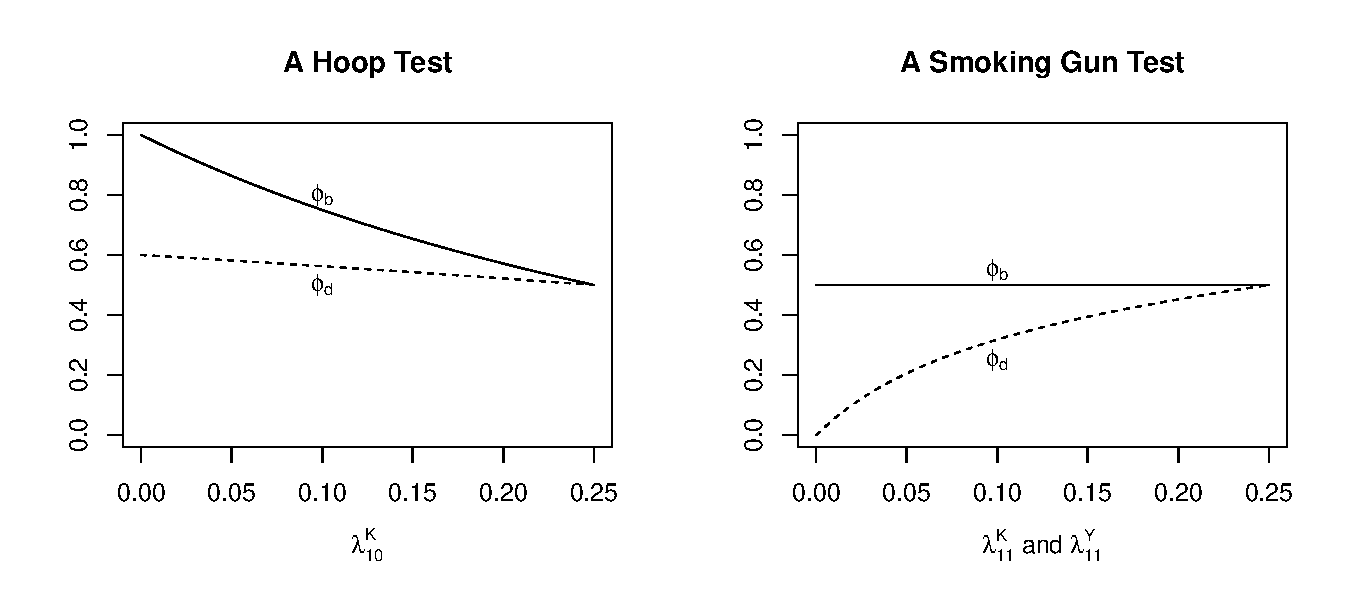
\includegraphics[width=.85\textwidth]{ii_files/figure-latex/phis-1} 

}

\caption{The probability of observing $K$ given causal type for different beliefs on lower-level causal effects. In the left figure, priors on all lower-level causal effects are flat except for the probability that $X$ has a negative effect on $K$. If we believe that it is unlikely that $X$ has a negative effect on $K$, $K$ becomes a `hoop' test for the proposition that a case is of type $b$. The righthand figure considers simultaneous changes in $\lambda_{11}^K$ and  $\lambda_{11}^Y$---the probabilities that $K=1$ regardless of $X$, and that $Y=1$  regardless of $K$, with flat distributions on all other lower-level effects. With $\lambda_{11}^K$, $\lambda_{11}^Y$ both close to 0, $K$ becomes a 'smoking gun' test for the proposition that $X$ has a positive effect on $Y$ ($b$ type).}\label{fig:phis}
\end{figure}

\hypertarget{assessing-probative-value-from-a-graph}{%
\section{Assessing probative value from a graph}\label{assessing-probative-value-from-a-graph}}

As we have argued, causal queries can be expressed as collections of combinations of nodal types (i.e., as collections of causal types) in a causal model. A nodal type is itself represented as an unobservable node in a model --- as a \(\theta^j\) pointing into node \(j\). Thus, causal inference in this framework is \emph{the use of observable nodes on a causal graph to assess the value of one or more unobserved nodes on a causal graph.} Placing our queries on the graph together with the observable nodes has the important advantage of allowing us to graphically identify the possibilities for learning about these queries: that is, to say which observable nodes are potentially informative about a given query.

To think through the logic of potential probative value, it is useful to distinguish among three different features of the world, as represented in our causal model: there are the things we want to learn about; the things we have already observed; and the things we could observe. As notation going forward, we let:

\begin{itemize}
\tightlist
\item
  \(\mathcal Q\) denote the collection of \(\theta^j\) nodes that define our \emph{query}; \(\mathcal Q\) cannot be directly observed so its values must be inferred;
\item
  \(\mathcal W\) denote a set of previously observed nodes in the causal model; and
\item
  \(\mathcal K\) denote a set of additional variables---clues---that we have not yet observed but could observe.
\end{itemize}

Now suppose that we seek to design a research project to investigate a causal question. How should the study be designed? Given that there are some features of the world that we have already observed, which additional clues should we seek to collect to shed new light on our question? In terms of the above notation, what we need to figure out is whether a given \(\mathcal K\) might be informative about---might provide additional leverage on---\(\mathcal Q\) given the prior observation of \(\mathcal W\).

To ask whether one variable (or set of variables) is informative about another is to ask whether the two (sets of) variables are, on average, \emph{correlated} with one another, given whatever we already know. Likewise, if two variables' distributions are fully \emph{independent} of one another (conditional on what else we have observed), then knowing the value of one variable can provide no new information about the value of the other.

Thus, asking whether a set of clues, \(\mathcal K\), is informative about \(\mathcal Q\) given the prior observation of \(\mathcal W\), is equivalent to asking whether \(\mathcal K\) and \(\mathcal Q\) are conditionally independent given \(\mathcal W\). That is, \(\mathcal K\) can be informative about \(\mathcal Q\) given \(\mathcal W\) only if \(\mathcal K\) and \(\mathcal Q\) are \emph{not} conditionally independent of one another given \(\mathcal W\).

As our discussion of conditional independence in Chapter \ref{models} implies, as long as we have built \(\mathcal Q\), \(\mathcal K\), and \(\mathcal W\) into our causal model of the phenomenon of interest, we can answer this kind of question by inspecting the structure of the model's DAG. In particular, what we need to go looking for are relationships of \emph{\(d\)-separation}. The following proposition, with only the names of the variable sets altered, is from \citet{pearl2009causality} (Proposition 1.2.4):

\textbf{Proposition 1:} If sets \(\mathcal Q\) and \(\mathcal K\) are \(d\)-separated by \(\mathcal W\) in a DAG, \(\mathcal G\), then \(\mathcal Q\) is independent of \(\mathcal K\) conditional on \(\mathcal W\) in every distribution compatible with \(\mathcal G\). Conversely, if \(\mathcal Q\) and \(\mathcal K\) are \emph{not} \(d\)-separated by \(\mathcal W\) in DAG \(\mathcal G\), then \(\mathcal Q\) and \(\mathcal K\) are dependent conditional on \(\mathcal W\) in at least one distribution compatible with DAG \(\mathcal G\).

We begin with a causal graph and a set of nodes on the graph (\(W\)) that we have already observed. Given what we have already observed, \emph{a collection of clue nodes, \(\mathcal K\), will be uninformative about the query nodes, \(\mathcal Q\), if \(\mathcal K\) is \(d\)-separated from \(\mathcal Q\) by \(\mathcal W\) on the graph.} (Equivalently, \(\mathcal K\), will be uninformative about \(\mathcal Q\), given that we have already observed \(\mathcal W\), if \(\mathcal K\) and \(\mathcal Q\) are conditionally independent given \(\mathcal W\).) When \(\mathcal W\) \(d\)-separates \(\mathcal K\) from \(\mathcal Q\), this means that what we have already observed already captures all information that the clues might yield about our query. On the other hand, if \(\mathcal K\) and \(\mathcal Q\) are \(d\)-connected (i.e., not \(d\)-separated) by \(W\), then \(K\) is \emph{possibly} informative about \(Q\). \(K\) is not \(d\)-separated from \(\mathcal Q\) by \(\mathcal W\).\footnote{This proposition is almost coextensive with the definition of a DAG. A DAG is a particular kind of dependency model (``graphoid'') that is a summary of a collection of ``independency statements'', \((I)\), over distinct subsets of \(\mathcal V\) (Pearl and Verma 1987), where \(I(\mathcal Q,\mathcal W,\mathcal K)\) means ``we learn nothing about \(\mathcal Q\) from \(\mathcal K\) if we already know \(\mathcal W\)''. More formally:
  \(I(\mathcal K, \mathcal W,\mathcal Q) \leftrightarrow P(\mathcal K,\mathcal Q|\mathcal W)=P(\mathcal K|\mathcal W)P(\mathcal Q|\mathcal W)\). A Directed Acyclic Graph Dependency model is one where the set of independencies corresponds exactly to the relations that satisfy \(d\)-separation (Pearl and Verma 1987, p376). Thus on DAG \(\mathcal G\), \(I(\mathcal K,\mathcal W,\mathcal Q)_{\mathcal G}\) implies that \(\mathcal K\) and \(\mathcal Q\) are \(d\)-separated by \(\mathcal W\).} Note, moreover, that under quite general conditions (referred to in the literature as the \emph{faithfulness} of a probability distribution) then there are at least \emph{some} values of \(\mathcal W\) for which \(\mathcal K\) \emph{will} be informative about \(\mathcal Q\).\footnote{Put differently, there will not be any conditional independencies that are \emph{not} captured in the DAG.}

Let us examine Proposition 1 in practice. We begin with the simplest case possible, and then move on to more complex models.

The very simplest probabilistic causal graph, shown in Figure \ref{fig:sepsimple}, has \(X\) influencing \(Y\), with \(X\) determined by a coin flip. If we want to know \(X\)'s effect on \(Y\), this query is defined solely in terms of \(Y\)'s nodal type, \(\theta^Y\). To help us conceptualize the more general point about informativeness for queries, we relabel \(\theta^Y\) as \(Q\) to emphasize the fact that this node represents our query.

\begin{figure}

{\centering 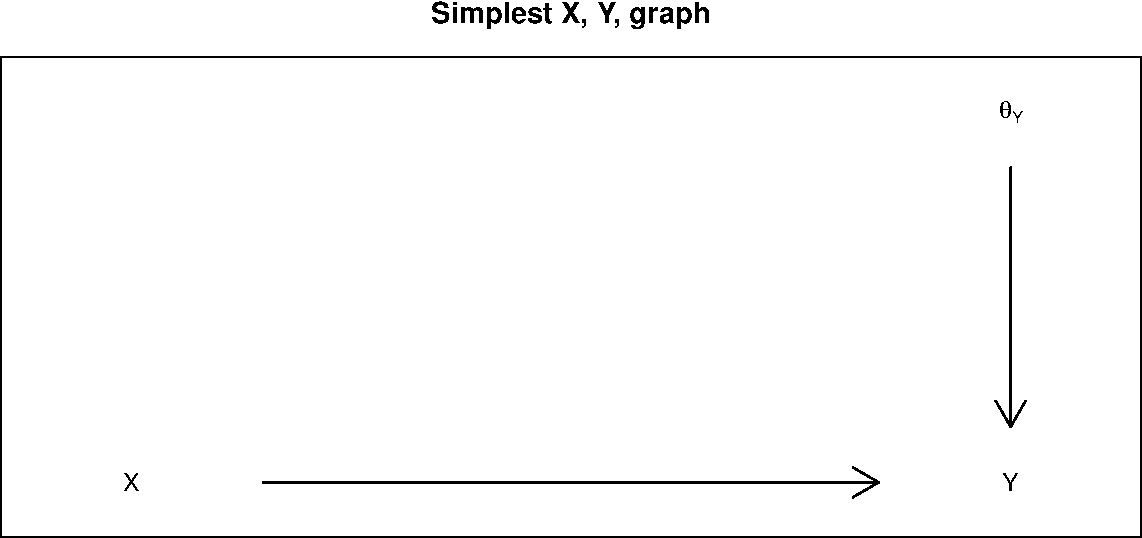
\includegraphics[width=.5\textwidth]{ii_files/figure-latex/sepsimple-1} 

}

\caption{A simple causal setup in which the effect of $X$ on $Y$ in a given case depends on the case's response type for $Y$.}\label{fig:sepsimple}
\end{figure}

Let us assume that we have observed nothing yet in this case and then ask what clue(s) might be informative about \(Q\), the node of interest. The other two nodes in the graph are \(X\) and \(Y\): these are thus the possible clues that we might go looking for in our effort to learn about \(Q\) (i.e., they are the possible members of \(\mathcal K\)).

First, can we learn about \(Q\) by observing \(X\)? We can answer this question by asking whether \(X\) is \(d\)-connected to \(Q\) on the graph given what we have already observed (which is nothing). We can see visually that there is no active path from \(X\) to \(Q\): the only path between \(X\) and \(Q\) is blocked by colliding arrow heads. Thus, \(X\) and \(Q\) are \(d\)-separated, meaning that \(X\) will not be informative about \(Q\): observing the value that a causal variable takes on in a case---having seen nothing else in the case---tells us nothing whatsoever about that variable's effect on the outcome. If we want to know whether a case is of a type in which the presence of natural resources would cause civil war, for instance, observing only that the case has natural resources does not help answer the question.

What, then, if we instead were to observe only \(Y\)? Is \(Y\) \(d\)-connected to \(Q\) given what we have already observed (which, again, is nothing)? It is: the arrow from \(Q\) to \(Y\) is an active path. Observing only the \emph{outcome} in a case does tell us something about causal effects. Returning to the natural resources and civil war example, observing only that a country has had a civil is informative about the case's causal type (the value of \(Q\)). In particular, it rules out the possibility that this is a case in which nothing could cause a civil war: that is, it excludes \(\theta^Y_{00}\) (i.e., \(c\)-type) as a possible value of \(Q\).

Suppose now, having observed \(Y\), that we were to consider also observing \(X\). Would we learn anything further about \(Q\) from doing so? We have already seen that observing \(X\) alone yields no information about \(Q\) because the two nodes are unconditionally \(d\)-separated, the path between them blocked by the colliding arrowheads at \(Y\). However, as we have seen, observing a collider variable (or one of its descendants) \emph{unblocks} the flow of information, generating relations of conditional dependence across the colliding arrowheads. Here, \(X\) and \(Q\) are \(d\)-connected by \(Y\): thus, if we have \emph{already} observed \(Y\), then observing \(X\) does confer additional information about \(Q\). Knowing only that a country has natural resources tells us nothing about those resources' effect on civil war in that country. But if we already know that the country has a civil war, then learning that the country has natural resources helps narrow down the case's possible response types. Having already used the observation of \(Y=1\) to rule out the possibility of \(\theta^Y_{00}\), observing \(X=1\) \emph{together with} \(Y=1\) allows us to additionally rule out the possibility that natural resources \emph{prevent} civil war, i.e., that \(Q=\theta^Y_{10}\).\footnote{That is, we can rule out that the case is an \(a\) type, or one with a negative causal effect.}

Finally, what if we observe \(X\) first and are considering whether to seek information about \(Y\)? Would doing so be informative? \(X\) does not \(d-\)separate \(Q\) from \(Y\); thus, observing \(Y\) will be informative about \(Q\). In fact, observing \(Y\) if we have already seen \(X\) is \emph{more} informative than observing \(Y\) alone. The reasoning follows the logic of collision discussed just above. If we observe \(Y\) having already seen \(X\), not only do we reap the information about \(Q\) provided by \(Y\)'s correlation with \(Q\); we simultaneously open up the path between \(X\) and \(Q\), learning additionally from the conditional dependence between \(X\) and \(Q\) given \(Y\).

We put Proposition 1 to work in a slightly more complex set of models in Figure \ref{fig:34graphs}. Here we investigate the informativeness of a clue that is neither \(X\) nor \(Y\). Each graph in Figure \ref{fig:34graphs} has four variables: \(X\); \(Y\); a possible clue, \(K\); and a node, \(Q\), representing the query (which we might also naturally think of as \(\theta^Y\)). We draw all 34 possible graphs with variables \(X\), \(Y\), \(K\), and \(Q\) for causal models in which (a) all variables are connected to at least one other variable, (b) \(X\) causes \(Y\) either directly or indirectly, and (c) \(Q\) is a direct cause of \(Y\) but is not caused by any other variable in the model and is thus exogenous. The title of each panel reports \(K\)'s conditional informativeness using principles of \(d\)-separation: it tells us when \(K\) is possibly informative about \(Q\) depending on whether \(X\), \(Y\), both or none are observed.\footnote{Note the ``possibly'' can be dropped under the assumption that the underlying probability model is ``stable'' \citep[section 2.9.1]{pearl2009causality} and with the interpretation that \(K\) is informative about \(Q\) for some, but not necessarily all, values of \(W\).}

\begin{figure}

{\centering 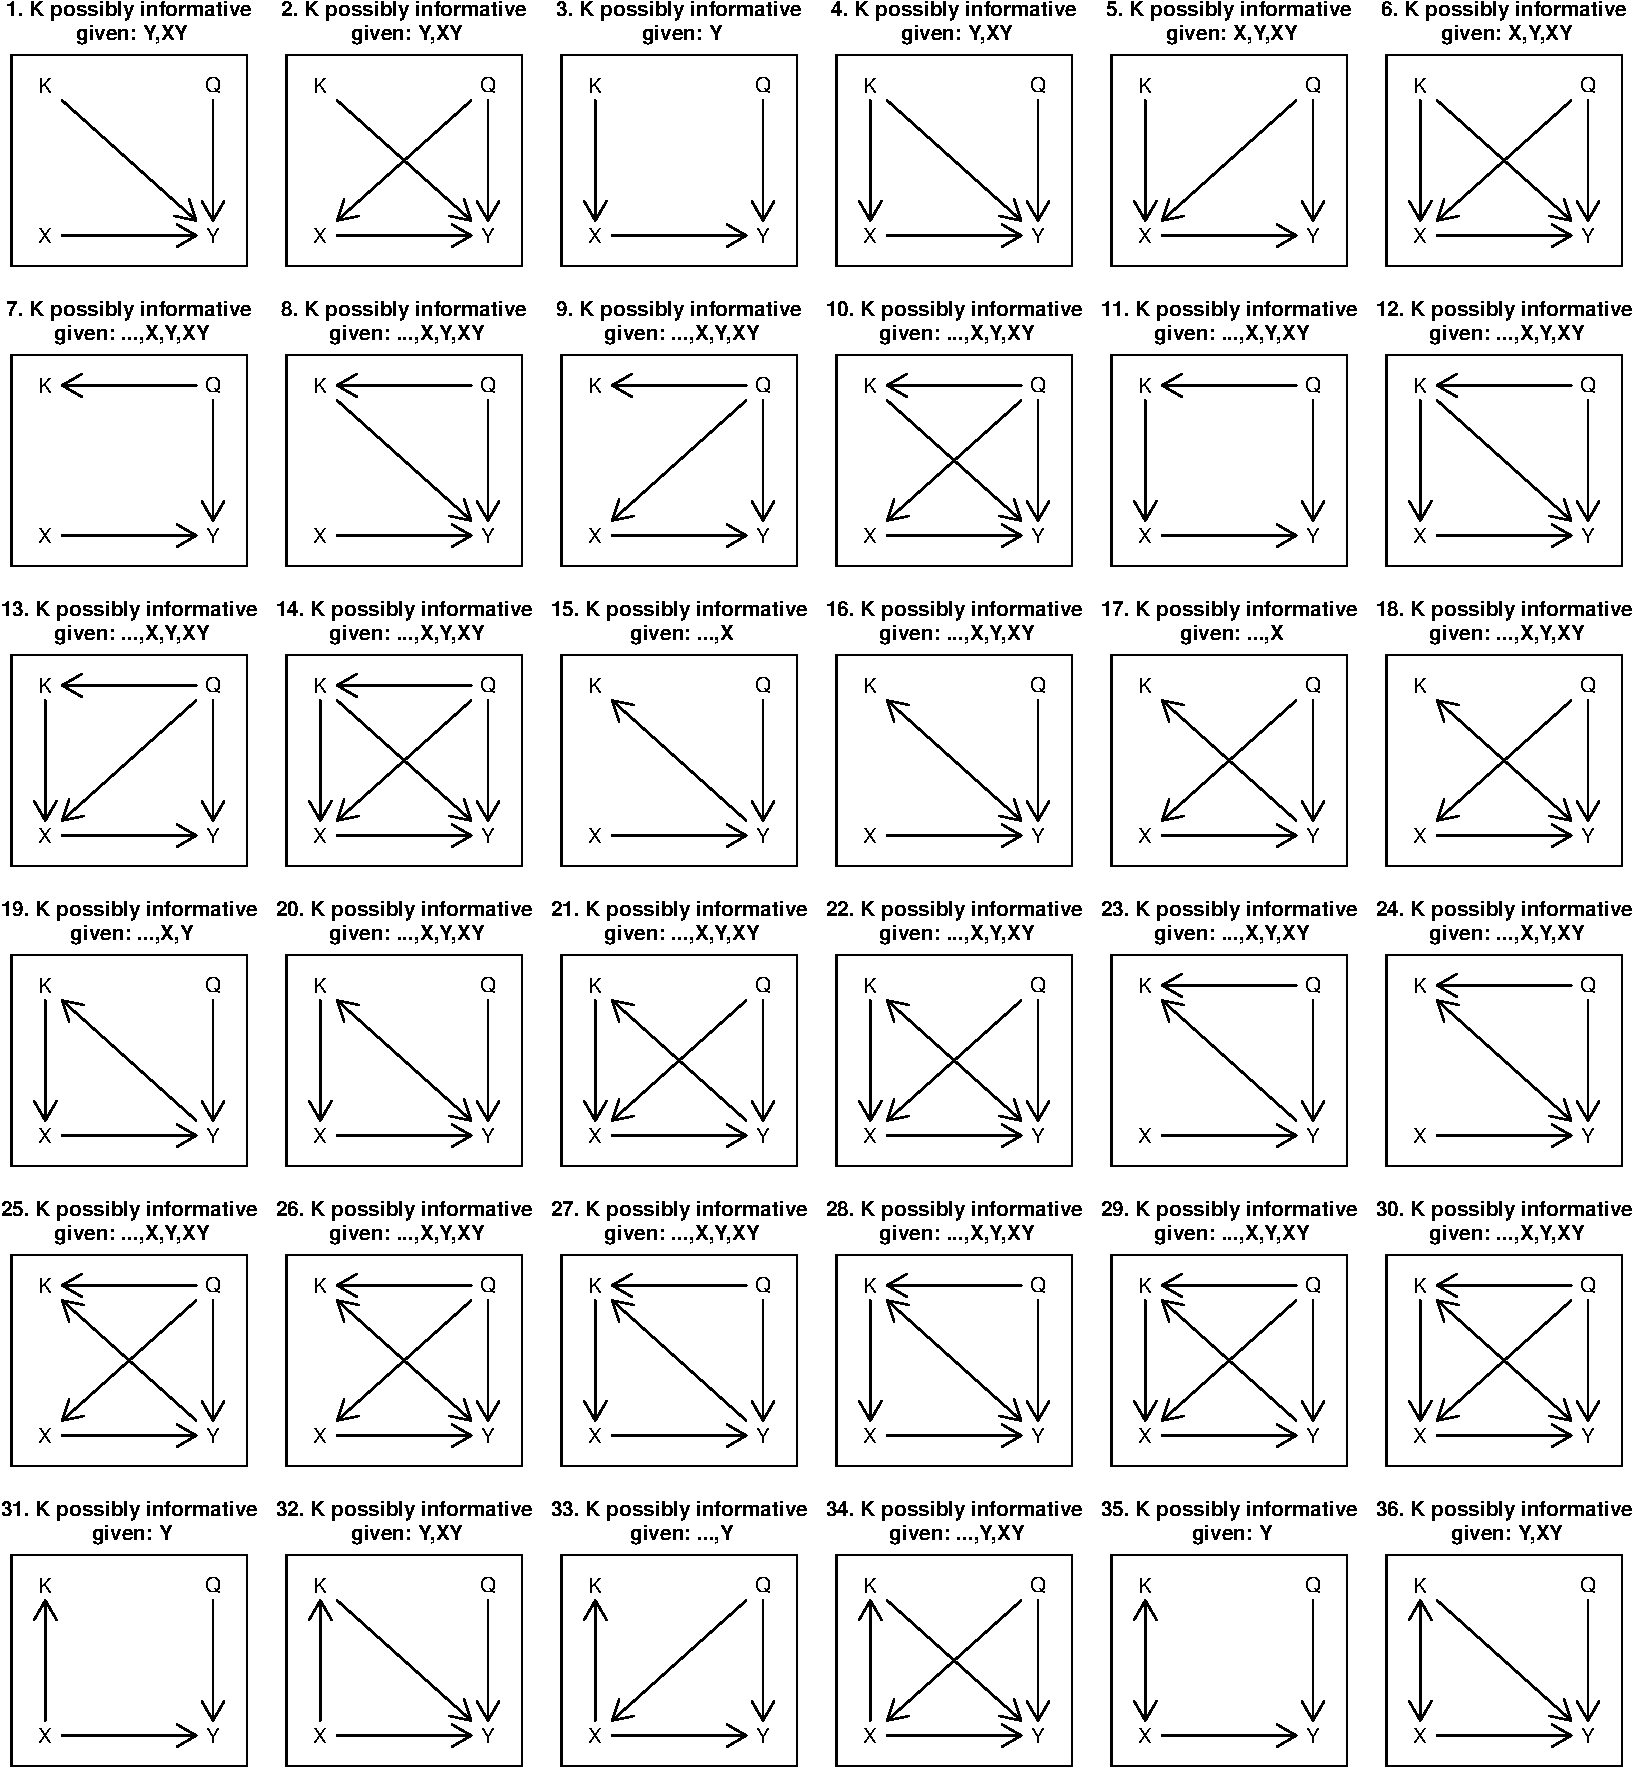
\includegraphics{ii_files/figure-latex/34graphs-1} 

}

\caption{All connected directed acyclic graphs over $X,Y,K,Q$, in which $Q$ is an exogenous variable that directly causes $Y$, and $X$ is a direct or indirect cause of $Y$. The title of each graph indicates the conditions under which $K$ can be informative about (i.e., is not $d$-separated from) $Q$, given the prior observation of $X$, $Y$, both, or neither (...).}\label{fig:34graphs}
\end{figure}

The results show us not just what kinds of variables can be informative about a case's response-type but also what combinations of observations yield leverage on case-level causal effects. A number of features of the graphs are worth highlighting:

\begin{itemize}
\item
  \textbf{Clues at many stages.} Process tracing has focused a great deal on observations that lie ``along the path'' between suspected causes and outcomes. What we see in Figure \ref{fig:34graphs}, however, is that observations at many different locations in a causal model can be informative about causal effects. We see here that \(K\) can be informative when it is pre-treatment (causally prior to \(X\)---e.g.~panel (3)), post-treatment but pre-outcome (that is, ``between'' \(X\) and \(Y\) as, e.g., in panel (20)), an auxiliary effect of \(X\) that itself has no effect on \(Y\) (e.g., in panel (19)), post-outcome (after \(Y\)---e.g., in panel (15)), or a joint effect of both the suspected cause and the outcome (e.g., panel (31)).
\item
  \textbf{Mediator Clues}. While clues that lie in between \(X\) and \(Y\) may be informative, they can only be informative under certain conditions. For instance, when a clue serves \emph{only} as a mediator in our model (i.e., its only linkages are being caused by \(X\) and being affected by \(Y\)) and \(Q\) only affects \(Y\), as in panels (20) and (21), the clue is only informative about \(Q\) if we have also observed the outcome, \(Y\). Of course, this condition may commonly be met---qualitative researchers usually engage in retrospective research and learn the outcome of the cases they are studying early on---but it is nonetheless worth noting why it matters: in this setup, \(K\) is unconditionally \(d\)-separated from \(Q\) by the collision at \(Y\); it is only by observing \(Y\) (the collider) that the path between \(K\) and \(Q\) becomes unblocked. (As we saw above, the very same is true for observing \(X\); it is only when we know \(Y\) that \(X\) is informative about \(Q\).)
\end{itemize}

In short, observations along causal paths are more helpful in identifying causal effects to the extent that we have measured the outcome. Importantly, this is not the same as saying that mediator clues are \emph{only} informative about causal effects where we have observed the outcome. Observing \(Y\) is necessary for the mediator to be informative about a \(Q\) term that is connected only to \(Y\). Observing a mediator without the outcome, however, could still be informative about the overall effect of \(X\) on \(Y\) by providing leverage on how the mediator responds to \(X\), which is itself informative about \(X\)'s effect on \(Y\) via the mediator.\footnote{In other words, the clue would then be providing leverage on a response-type variable pointing into the mediator itself.} Moreover, observing the mediator could be informative without the observation of \(Y\) if, for instance, \(Q\) also points into \(K\) itself or into a cause of \(K\). As we discuss below, the clue then is informative as a ``symptom'' of the case's response type, generating learning that does not hinge on observing the outcome.

\begin{itemize}
\tightlist
\item
  \textbf{Symptoms as clues.} Some clues may themselves be affected by \(Q\): that is to say, they may be symptoms of the same conditions that determine causal effects in a case. For instance, in our illustrative model involving government survival, government sensitivity functions as a response-type variable for the effect of a free press (\(X\)) on government removal (\(Y\)): a free press only generates government removal when the government is non-sensitive to public opinion. Sensitivity to public opinion thus represents our query variable, \(Q\), if we seek to learn whether a free press causes government removal in a case. While it may not be possible to observe or otherwise measure the government's sensitivity, there may be \emph{consequences} of government sensitivity that are observable: for instance, whether government officials regularly consult with civil-society actors on policy issues. While consultations would not be part of the causal chain generating the free press's effect, observing consultations (or the lack of them) would be informative about that effect because consultations are a symptom of the same conditions that enable the effect.
\end{itemize}

We see that \(K\) is a child or descendant of \(Q\) in several of the graphs in Figure \ref{fig:34graphs}: \(Q\) directly causes \(K\) in panels (7) through (14), (17), (18), (25)-(30), (33), and (34); \(Q\) causes (K) only indirectly through \(X\) in panels (22) through (24); \(Q\) causes (K) only indirectly through \(Y\) in panels (15), (16), and (31); and \(Q\) causes \(K\) only indirectly through \(X\) and through \(Y\) in panel (32). We can then use the principle of \(d\)-separation to figure out when the symptom clue is potentially informative, given what we have already observed. It is easy to see that \(K\) is potentially informative, no matter what we have already observed, if \(K\) is directly affected by \(Q\); there is nothing we could observe that would block the \(Q \rightarrow K\) path. Thus, \(Q\)'s ``symptom'' can, in this setup, contain information about type above and beyond that contained in the \(X\) and \(Y\) values. However, where \(Q\) affects \(K\) only through some other variable, observing that other variable renders \(K\) uninformative by blocking the \(Q\)-to-\(K\) path. For instance, where \(Q\) affects \(K\) indirectly through \(X\), once we observe \(X\), we already have all the information about \(Q\) that would be contained in \(K\).

\begin{itemize}
\tightlist
\item
  \textbf{Surrogates as clues.} Clues may be consequences of the outcome, as in graphs (15) and (16). If \(K\) is a consequence \emph{only} of \(Y\), then it will contain no new information about \(Q\) where \(Y\) is already known. However, in situations where the outcome has not been observed, \(K\) can act as a ``surrogate'' for the outcome and thus yield leverage on \(Q\) \citep{frangakis2002principal}. A researcher might, for instance, seek to understand causal effects on an outcome that is difficult to directly observe: consider, for instance, studies that seek to explain ideational change. Ideas themselves, the \(Y\) in such studies, are not directly observable. However, their consequences---such as statements by actors or policy decisions---will be observable and can thus serve as informative surrogates for the outcome of interest.
\end{itemize}

Clues may similarly serve as surrogates of a cause, as in graphs (19) and (22). Here \(X\) causes \(K\), but \(K\) plays no role in the causal process generating \(Y\). \(K\) is of no help if we can directly measure \(X\) since the latter \(d\)-separates \(K\) from \(Q\). But if an explanatory variable cannot be directly measured---consider, e.g., ideas or preferences as causes---then its consequences, including those that have no relationship to the outcome of interest, can provide leverage on the case-level causal effect.

Clues can also be a consequence of both our suspected cause and the outcome of interest, thus serving as what we might call ``double surrogates,'' as in panels (31) and (32). Here \(X\) is a direct cause of \(Y\), and \(K\) is a joint product of \(X\) and \(Y\). A double surrogate can be informative as long as we have not already observed both \(X\) and \(Y\). Where data on either \(X\) or \(Y\) are missing, there is an open path between \(K\) and \(Q\). If we have already observed both, however, then there is nothing left to be learned from \(K\).

\begin{itemize}
\tightlist
\item
  \textbf{Instruments as clues.} Clues that are causally prior to an explanatory variable, and have no other effect on the outcome, can sometimes be informative. Consider, for instance, graph (3). Here \(K\) is the only cause of \(X\). It can thus serve as a proxy. If we have seen \(X\), then \(X\) blocks the path between \(K\) and \(Q\), and so \(K\) is unhelpful. \(K\) can be informative, though, if we have \emph{not} observed \(X\). Note that informativeness here still requires that we observe \(Y\). Since \(Y\) is a collider for \(Q\) and the \(K \rightarrow X \rightarrow\) chain, we need to observe \(Y\) in order to \(d\)-connect \(K\) to \(Q\).
\end{itemize}

A rather different setup appears in graph (5), where both \(K\) and \(Q\) cause \(X\). Now the conditions for \(K\)'s informativeness are broader. Observing \(X\) still makes \(K\) uninformative as a proxy for \(X\) itself. However, because \(X\) is a collider for \(K\) and \(Q\), observing \(X\) \emph{opens up} a path from \(K\) to \(Q\), rendering a dependency between them. Still, we have to observe at least one of \(X\) or \(Y\) for the instrument to be informative here. This is because both of \(K\)'s paths to \(Q\) run through a collision that we need to unblock by observing the collider. For one path, the collider is \(X\); for the other path, the collider is \(Y\).\footnote{As a simple example one might imagine a system in which \(X = K\) if \(q \in {a,b}\) and \(X = 1-K\) if \(q \in {c,d}\). Then if we observe, say, \(X=Y=K=1\), we can infer that \(q = b\). Another way to think about what is happening in graph (5) is that \(K\) is providing information about the \emph{assignment process}. In this graph, the causal effect (\(Y\)'s potential outcomes, determined by \(Q\)) is also a partial determinant of the assignment of cases to values on \(X\). In terms of cross-case correlational inference, then, we would think of this as a situation of confounding. Observing another cause of \(X\), then, allows us to more fully characterize the process of assignment.}

Other patterns involving instrumentation are also imaginable, though not graphed here. For example, we might have a causal structure that combines instrumentation and surrogacy. Suppose that \(X\) is affected by \(Q\) and by an unobservable variable \(\theta_X\); and that \(\theta_X\) has an observable consequence, \(K\). Then \(K\), though not a cause of \(X\), is a ``surrogate instrument'' \citep{hernan2006instruments} as it is a descendant of an unobserved instrument, \(U\), and thus allows us to extract inferences similar to those that we could draw from a true instrument.

\begin{itemize}
\tightlist
\item
  \textbf{Confounders as clues.} In several of the graphs, \(K\) is a confounder in that it is a direct cause of both \(X\) and \(Y\) (panels (4), (6), (12), and (14)). Let us focus on graph (4), which isolates \(K\)'s role as a confounder. Here \(K\) can be informative via two possible paths. First, if \(X\) is not observed but \(Y\) is, then \(K\) is \(d\)-connected to \(Q\) along the path \(K \rightarrow X \rightarrow Y \leftarrow Q\). \(K\) is in this sense serving as a proxy for \(X\), with its path to \(Q\) opened up by the observation of the collider, \(Y\). Second, with \(Y\) observed, \(K\) can provide information on \(Q\) via the more direct collision, \(K \rightarrow Y \leftarrow Q\). If \(X\) \emph{is} observed, then the first path is blocked, but the second still remains active. As with any pre-outcome variable, for a confounder clue to provide purchase on \(Y\)'s response type, \(Y\) itself must be observed.
\end{itemize}

In a sense, then, the role of confounders as clues in case-level inference is the mirror image of the role of confounders as covariates in cross-case correlational inference. In a correlational inferential framework, controlling for a variable in \(K\)'s position in graph (5) renders the \(X, Y\) correlation (which we assume to be observed) informative about \(X\)'s average causal effect. When we use confounders as evidence in within-case inference, it is our observations of other variables that determine how informative the confounder \emph{itself} will be about \(X\)'s causal effect.

It is important to be precise about the kinds of claims that one can make from graphs like those in Figure \ref{fig:34graphs}. The graphs in this figure allow us to identify informativeness about an unobserved node \(Q\) that is a parent of \(Y\). This setup does not, however, capture all ways in which clues can be informative about the causal effect of \(X\) on \(Y\) or about other causal queries of interest. For instance, as noted above, even if a clue is uninformative about a \(Q\) node pointing into \(Y\), it may still help establish whether \(X\) causes \(Y\): the statement that \(X\) causes \(Y\) will for some graphs be a statement about a \emph{collection} of nodes that form the set of query variables \(\mathcal Q\). This is the case, for instance, in any graph of the form \(X \rightarrow M \rightarrow Y\), where we are interested not just in \(Y\)'s response to \(M\) (the mediator) but also in \(M\)'s response to \(X\). Of interest, thus, are not just a \(Q^Y\) response-type node pointing into \(Y\) but also a \(Q^M\) response-type node that is a parent of \(M\). Observations that provide leverage on either \(Q\) term will thus aid an inference about the overall causal effect. A clue \(K\) that is \(d-\)separated from \(Q^Y\) may nevertheless be informative about \(X\)'s effect on \(Y\) if it is not \(d-\)separated from \(Q^M\); this opens up a broader range of variables as informative clues.

Additionally, as our discussion in Chapter \ref{models} makes clear, queries other than the case-level causal effect---such as average causal effects, actual causes, and causal paths---involve particular features of context: particular sets of exogenous nodes as members of our query set, \(\mathcal Q\). Thus, even for the same causal model, informativeness will be defined differently for each causal question that we seek to address. The broader point is that we can identify what kinds of observations may address our query if we can place that query on a causal graph and then assess the graph for relationships of \(d\)-separation and -connection.

Further, we emphasize that a DAG can only tell us when a clue \emph{may} be informative (conditional some prior observation): \(d-\)connectedness is necessary but not sufficient for informativeness. This fact derives directly from the rules for drawing a causal graph: the absence of an arrow between two variables implies that they are \emph{not} directly causally related, while the presence of an arrow does not imply that they always are. As we saw in our analysis of the government-removal example in Chapter \ref{models}, whether variables connected to one another by arrows in the original DAG were in fact linked by a causal effect depended on the context. Likewise, whether a clue \(K\) is in fact informative may depend on particular values of \(\mathcal W\)---the variables that have already been observed. As a simple example, let \(q = k_1w + (1-w)k_2\), where \(W\) is a variable that we have already observed and \(K_1\) and \(K_2\) are clues that we might choose to observe next. Here, if \(w=1\) then learning \(K_1\) will be informative about \(Q\), and learning \(K_2\) will not; but if \(w=0\), then \(K_1\) will be uninformative (and \(K_2\) informative).

In general, then, graphical analysis alone can help us exclude unhelpful research designs, given our prior observations and a fairly minimal set of prior beliefs about causal linkages. This is no small feat. But identifying those empirical strategies that will yield the \emph{greatest} leverage requires engaging more deeply with our causal model, as we show in detail in our discussion of clue-selection in Chapter \ref{clue}.

\hypertarget{principles-of-learning}{%
\section{Principles of learning}\label{principles-of-learning}}

While \texttt{CausalQueries} can implement process-tracing inference for us, it is helpful for researchers to be able to reason their way through what is happening ``under the hood.'' We provide here some core principles and intuitions for thinking through the features of models and queries that influence whether and how much we can learn from within-case observations.

\hypertarget{a-dag-alone-does-not-guarantee-probative-value-for-a-single-case}{%
\subsection{A DAG alone does not guarantee probative value for a single case}\label{a-dag-alone-does-not-guarantee-probative-value-for-a-single-case}}

A DAG puts qualitative structure on causal relations but quantitative implications depend on the beliefs over causal types. In general, learning from new data requires that, conditional on known data, the probability of a new data pattern is different depending on whether or not the query is true. With flat priors this condition may not hold for many queries of interest.

To illustrate, suppose that we are interested in whether \(X\) caused \(Y\) and we posit a simple \(X \rightarrow M \rightarrow Y\) model with flat priors over \(\theta^M\) and \(\theta^Y\). Now we would like to conduct process tracing and observe \(M\) to tell us about the effect of \(X\) on \(Y\) in a case with \(X=Y=1\) case.

Does the observation of \(M\) provide leverage on whether \(X=1\) caused \(Y=1\)?

It does not. We can learn nothing about \(X\)'s effect on \(Y\) from observing \(M\).

To see why, consider that there are two causal types that will satisfy the query, \(X=1\) caused \(Y=1\). Those are the types \(\theta^X_1 \theta^M_{01} \theta^Y_{01}\) and \(\theta^X_1 \theta^M_{10} \theta^Y_{10}\): either linked positive effects or linked negative effects could generate an overall positive effect of \(X\) on \(Y\). Moreover, with flat priors over nodal types, these causal types are equally likely. Now, think about what we would conclude if we collected process data and observed \(M=1\) in the \(X=Y=1\) case. This observation would rule out various ways in which \(X\) did not cause \(Y\) but it also rules out one way in which the query could be satisfied: the causal type with linked negative effects. And what if we observed, instead, \(M=0\)? This would have similar implucations, this time ruling out the other way in which the query could be satisfied: linked positive effects. Intuitively we would update the same way no matter what we find, which means we must not be updating at all.

More formally, conditional on observing \(X=1, Y=1\) our prior that \(X\) caused \(Y\) is:

\[\frac{\lambda^M_{01}\lambda^Y_{01}+ \lambda^M_{10}\lambda^Y_{10}}{(\lambda^M_{01}+\lambda^M_{11})(\lambda^Y_{01}+ \lambda^Y_{11})+ (\lambda^M_{10}+\lambda^M_{00})(\lambda^Y_{10}+ \lambda^Y_{11}) }\]

Our posterior on observing \(M=1\) is:

\[\frac{\lambda^M_{01}\lambda^Y_{01}}{(\lambda^M_{01}+\lambda^M_{11})(\lambda^Y_{01} + \lambda^Y_{11})}\]
it is easy to see these are equal with flat priors (\(\lambda^j_{ab}=\lambda^{j*}\) for all \(a,b\)). What we can see from the comparison is that when we observe data we rule out half the types consistent with the data (denominator) but also rule out half the types consistent with the query \emph{and} data (numerator) .

It is worth noting however that informative priors on \emph{either} \(\theta^M\) or \(\theta^Y\), would help here.

More generally, what we need at the level of priors depends on the query. Suppose that we start with the model, \(X \rightarrow M \rightarrow Y\), and formulate the following query: does \(X\) have a positive effect on \(Y\) that runs through a chain of positive effects via \(M\)? We can learn about this query without any informative priors over nodal types because of the way in which the query itself restricts the type space. Since the query is not satisfied if negative mediating effects are operating, we will update to probability 0 on the query for any observation that violates \(X=M=Y\), and we will update upwards on the query for any observation of \(X=M=Y\).

\hypertarget{learning-requires-uncertainty}{%
\subsection{Learning requires uncertainty}\label{learning-requires-uncertainty}}

While case-level inference from within-case evidence requires informative priors about nodal types, there is also such a thing as \emph{too much} information -- or, put differently, as insufficient uncertainty about causal relations. Suppose, for instance, that our beliefs are such that \(X\) always has a positive effect on \(M\) in an \(X \rightarrow M \rightarrow Y\) model. Consider, further, that we already know that \(X=1\) in a case. In that situation, nothing can be learned by observing \(M\) since the prior observation of \(X\) already reveals \(M\)'s value given our prior beliefs.

To take a less extreme example, suppose that our priors put a \emph{very high probability} on \(X\)'s having a positive effect on \(M\) and that, again, we already know that \(X=1\) in a case. In that situation, we should \emph{expect} to learn very little from observing \(M\) since we believe that we are very likely to see \(M=1\), given that we already know \(X=1\). It is true that our beliefs will shift \emph{if} we look for \(M\) and find the unexpected value of \(M=0\). But because that data-realization is highly unlikely, we should expect the learning from observing \(M\) to be minimal.

We address the concept of expected learning more systematically in Chapters \ref{clue} and \ref{caseselection}, but our general point here is that, we will learn more from process-tracing evidence, to the extent that (a) we know enough about causal relations in a domain to know how to make causal sense of the evidence we find, but (b) we do not know so much that that evidence can be largely predicted from what we have already observed.

\hypertarget{the-more-specific-the-query-the-more-difficult-it-is-to-gain-leverage}{%
\subsection{The more specific the query the more difficult it is to gain leverage}\label{the-more-specific-the-query-the-more-difficult-it-is-to-gain-leverage}}

It is difficult to get empirical leverage on very highly queries.

To illustrate, suppose that we start with the two-path model, \(X \rightarrow M \rightarrow Y \leftarrow X\), and formulate the following query: does \(X\) have a positive effect on \(Y\) that runs through a chain of positive effects via \(M\)? Suppose that we begin with flat priors over all nodal types. Intuitively, this seems like exactly the kind of question for which an observation of \(M\) is the perfect empirical strategy. And that intuition is, in a sense, correct: we can indeed learn about the query by observing \(M\). Seeing \(M=1\) in an \(X=Y=1\) case, for instance, would be evidence consistent with the query while seeing \(M=0\) in that same case would be inconsistent with the query.

Yet, we will only learn very modestly about the query from this observation. The reason is that the query itself has a very low prior probability. It may, in fact, not be obvious at first glance just how unlikely our query is in our priors. At first glance, it looks as though all we are asking is whether there exist positive effects running through one of the two causal paths in the model. However, consider the joint nodal-type probabilities implied by the query. First, the query requires \(X\) to have a positive effect on \(M\), to which our priors give only a \(25\%\) chance In addition, the query puts a very narrow constraint on \(Y\)'s possible nodal types: to satisfy the query, \(Y\) must have a nodal type in which \(M\) has a positive effect on \(Y\) when \(X\) does not change, and in which \(X\) does not have a positive effect on \(Y\) unless \(M\) changes from \(0\) to \(1\). This pair of conditions is met by only 2 of \(Y\)'s 16 nodal types, implying a \(12.5\%\) chance. The prior on the query itself is, thus, \(0.25 \times 0.125 = 0.03125\). Thus, while observing \(M=0\) takes the probability of the query down to \(0 \%\), we started out very close to 0\%! Observing \(M=1\) results in only a small uptick, to about \(6\%\) because there remain many type combinations consistent with M=1 but that do not fit through the needle-eye of this query.

In sum, what seems intuitively like a simple question will sometimes be a very unlikely query. What makes this query so unlikely is the interplay between the query itself and the model. The model allows for a \emph{wide} range of causal combinations (e.g., \(Y\)'s 16 nodal types), spreading prior weight thinly across those many possibilities, while the query zeroes in on a couple of \emph{particular} combinations that, in our priors, each have very low probability.

\hypertarget{population-level-uncertainty-does-not-alter-case-level-causal-inference}{%
\subsection{Population-level uncertainty does not alter case-level causal inference}\label{population-level-uncertainty-does-not-alter-case-level-causal-inference}}

In the procedure described for process tracing in this chapter (and different to what we introduce in Chapter \ref{ptapp}) we assume that \(\lambda\) is known and we do not place uncertainty around it.

This might appear somewhat heroic, but in fact for single case inference it is without loss of generality. The expected inferences we would make for any query accounting for priors is the same as the inferences we if we use the expectation only.

To see this, let \(\pi_j\) denote the probability of observing causal type \(j\) and \(p(D)\) the probability of observing data realization \(D\). Say that \(j \in D\) if type \(j\) produces data type \(D\) and say \(j \in E\) if causal type \(j\) is an element of the query set of interest.
The posterior on a query \(E\) given data \(D\) given prior over \(\pi\), \(p(\pi)\) is:

\[\Pr(E | D) = \int_\pi  \frac{\sum_{j \in E \cap D}\pi_j}{\sum_{j \in D}\pi_j} f(\pi)d\pi\]

However, since for any \(\pi\), \(\sum_{j \in D}\pi_j = p(D)\) we have:

\[\Pr(E | D) = \int_\pi  \sum_{j \in E \cap D}\pi_j f(\pi)d\pi/p(D) = \sum_{j \in  E \cap D} \overline{\pi}_j/p(D)\]
For instance in an \(X \rightarrow Y\) model, if we observe \(X=Y=1\) then \(D\) consists of causal types \(D={(\theta^X_1, \theta^Y_{01}), (\theta^X_1, \theta^Y_{11})})\) and the query set for ``\(X\) has a positive effect on \(Y\)'' consists of \(E={(\theta^X_1, \theta^Y_{01}), (\theta^X_0, \theta^Y_{01})})\). Let \(\pi_1\), \(\pi_2\) denote the priors on the two elements of \(D\). We then have:

\[\Pr(E | D) =  \frac{\pi_1}{\pi_1 + \pi_2}\]

\hypertarget{ptapp}{%
\chapter{Process Tracing Application}\label{ptapp}}

\begin{headerbox}
We apply the causal-model-based approach to process tracing to a major substantive issue in comparative politics: the relationship between inequality and democratization. Drawing on case level data, we use qualitative restrictions on causal types together with flat priors to draw inferences about the probability with which inequality facilitated or hindered democratization.

\end{headerbox}

In this chapter, we demonstrate how causal-model-based process-tracing works using real data. We undertake this illustration on a substantive issue that has been of central interest to students of comparative politics for decades: the causes of democratization. As the literature and range of arguments about democratization are vast, we focus on just a piece of the debate---specifically on causal claims about the relationship between economic inequality and democratization, with particular attention to the work of \citet{boix2003democracy}, \citet{acemoglu2005economic}, and \citet{haggard2012inequality}. In this chapter, we demonstrate process tracing with causal models, while in a later chapter we demonstrate the integration of process-tracing with correlational analysis. Our focus in this chapter is on using process tracing to assess \emph{the case-level causal effect of inequality on democracy.}

\hypertarget{inequality-and-democratization-the-debate}{%
\section{Inequality and Democratization: The Debate}\label{inequality-and-democratization-the-debate}}

Sociologists, economists, and political scientists have long theorized and empirically examined the relationship between inequality and democracy (e.g., \citet{dahl1973polyarchy}, \citet{bollen1985political}, \citet{acemoglu2005economic}, \citet{boix2003democracy}, \citet{ansell2014inequality}). In recent years, the work of \citet{boix2003democracy}, \citet{acemoglu2005economic}, and \citet{ansell2014inequality} represent major theoretical advances in specifying when and how inequality might generate transitions to democracy (as well as its persistence, which we bracket here). The first and third of these books also provide large-n cross-national and historical tests of their theories' key correlational predictions. \citet{haggard2012inequality}, moreover, derive causal process observations from a large number of ``Third Wave'' cases of democratization in order to examine these theories' claims about the centrality of distributional issues to regime change. We provide a very condensed summary of the core logic of \citet{boix2003democracy} and \citet{acemoglu2005economic} before seeking to translate that logic into a causal model for the purposes of process tracing, using a transformed version of Haggard and Kaufman's causal-process data.

We briefly summarize the core logics of and differences among these three sets of arguments here, bracketing many of their moving parts to focus on the basic theorized relationship between inequality and democracy. Both Boix's and Acemoglu and Robinson's theories operate within a Meltzer-Richard \citep{meltzer1981rational} framework in which, in a democracy, the median voter sets the level of taxation-and-transfer and, since mean income is higher than median income, benefit from and vote for a positive tax rate, implying redistribution from rich to poor. The poorer the median voter, the more redistribution she will prefer. Democracy, with its poorer median voter, thus implies greater redistribution than (rightwing) authoritarianism---a better material position from the poor at the expense of the rich elite. Thus, in each of these approaches, struggles over political regimes are conflicts over the distribution of material resources.

In Boix's model, the poor generally prefer democracy for its material benefits. When they mobilize to demand regime change, the rich face a choice as to whether to repress or concede, and they are more likely to repress as inequality is higher since, all else equal, they have more to lose from democracy. Thus, with the poor always preferring democracy over rightwing authoritarianism, inequality reduces the prospects for democratization.

In Acemoglu and Robinson's model, inequality simultaneously affects the expected net gains to democracy for both rich and poor. At low levels of inequality, democracy is relatively unthreatening to the elite, as in Boix, but likewise of little benefit to the poor. Since regime change is costly, the poor do not mobilize for democracy when inequality is low, and democratization does not occur. At high levels of inequality, democracy is of great benefit to the poor but has high expected costs for the elite; thus, democratization does not occur because the elite repress popular demands for regime change. In Acemoglu and Robinson's model, democracy emerges only when inequality is at middling levels: high enough for the poor to demand it and low enough for the rich to be willing to concede it.

Ansell and Samuels, finally, extend the distributive politics of regime change in two key ways. First, they allow for a two-sector economy, with a governing elite comprising the landed aristocracy and an urban industrial elite excluded from political power under authoritarian institutions. Total inequality in the economy is a function of inequality in the landed sector, inequality in the industrial sector, and the relative size of each. Second, authoritarian (landed) elites can tax the industrial bourgeoisie, thus giving the industrial elite an incentive to seek constraints on autocratic rule. Third, in Ansell and Samuels' model, rising industrial inequality means a rising industrial elite, generating a larger gap between them and industrial workers, though the industrial masses are richer than the peasantry. A number of results follow, of which we highlight just a couple. Rising land inequality reduces the likelihood of bourgeois rebellion by giving the landed elite greater repressive capacities and increasing their expected losses under democracy. As industrial inequality rises, however, the industrial elite have more to lose to confiscatory taxation and thus greater incentive to push for partial democracy (in which they have the ability to constrain the government, though the poor remain politically excluded) as well as greater resources with which to mobilize and achieve it. Full democracy, brought on by joint mass and bourgeois rebellion, is most likely as the industrial sector grows in relative size, giving the urban masses more to lose to autocratic expropriation and more resources with which to mobilize and rebel.

These three theoretical frameworks thus posit rather differing relationships between inequality and democracy. Taking these theoretical logics as forms of background knowledge, we would consider it possible that inequality reduces the likelihood of democracy or that it increases the likelihood of democracy. Yet one feature that all three theories have in common is a claim that distributional grievances drive demands for regime change. Moreover, in both Boix and Acemoglu and Robinson, less economically advantaged groups are, all else equal, more likely to demand democracy the worse their relative economic position. Ansell and Samuels' model, on the other hand, suggests that relative deprivation may cut both ways: while poorer groups may have more to gain from redistribution under democracy, better-off groups have more to fear from confiscatory taxation under autocracy. In all three frameworks, \emph{mobilization} by groups with material grievances is critical to transitions to democracy: elites do not voluntarily cede power.

In their qualitative analysis of ``Third Wave'' democratizations, Haggard and Kaufman point to additional factors, aside from inequality, that may generate transitions. Drawing on previous work on 20th century democratic transitions (e.g., \citet{huntington1993third}, \citet{linz1996problems}), they pay particular attention to international pressures to democratize and to elite defections.

\hypertarget{a-structural-causal-model}{%
\section{A Structural Causal Model}\label{a-structural-causal-model}}

We now need to express this background knowledge in the form of a structural causal model. Suppose that we are interested in the case-level causal effect of inequality on democratization of a previously autocratic political system. Suppose further, to simplify the illustration, that we conceptualize both variables in binary terms: inequality is either high or low, and democratization either occurs or does not occur. This means that we want to know, for a given case of interest, whether high inequality (as opposed to low inequality) causes democracy to emerge, prevents democracy from emerging, or has no effect (i.e., with democratization either occurring or not occurring independent of inequality). We can represent this query in the simple, high-level causal model shown in Figure \ref{fig:dagdemochigh}. Here, the question, ``What is the causal effect of high inequality on democratization in this case?'' is equivalent to asking what the value of \(\theta^D\) is in the case, where the possible values are \(\theta_{00}^D, \theta_{01}^D, \theta_{10}^D\), and \(\theta_{11}^D\). We assume here that the case's nodal type, \(\theta^D\), is not itself observable, and thus we are in the position of having to make inferences about it.

Drawing on the grammar of causal graphs discussed in Chapter \ref{models}, we can already identify possibilities for learning about \(\theta^D\) from the other nodes represented in this high-level graph. Merely observing the level of inequality in a case will tell us nothing since \(I\) is not \(d-\)connected to \(\theta^D\) if we have observed nothing else. On the other hand, only observing the outcome---regime type---in a case \emph{can} give us information about \(\theta^D\) since \(D\) \emph{is} \(d-\)connected to \(\theta^D\). For instance, if we observe \(D=1\) (that a case democratized), then we can immediately rule out \(\theta_{00}^D\) as a value of \(\theta^D\) since this type does not permit democratization to occur. Further, conditional on observing \(D\), \(I\) is now \(d-\)connected to \(\theta^D\): in other words, having observed the outcome, we can additionally learn about the case's type from observing the status of the causal variable. For example, if \(D=1\), then observing \(I=1\) allows us additionally to rule out the value \(\theta_{10}^D\) (a negative causal effect).

Now, observing just \(I\) and \(D\) alone will always leave two nodal types in contention. For instance, seeing \(I=D=1\) (the case had high inequality and democratized) would leave us unsure whether high inequality caused the democratization in this case (\(\theta^D=\theta_{01}^D\)) or the democratization would have happened anyway (\(\theta^D=\theta_{11}^D\)). This is a limitation of \(X, Y\) data that we refer to in \citet{humphreys2015mixing} as the ``fundamental problem of type ambiguity.'' Note that this does not mean that we will be left indifferent between the two remaining types. Learning from \(X, Y\) data alone---narrowing the types down to two---can be quite significant, depending on our priors over the distribution of types. For example, if we previously believed that a \(\theta_{00}^D\) type (cases in which democracy will never occur, regardless of inequality) was much more likely than a \(\theta_{11}^D\) type (democracy will always occur, regardless of inequality) and that positive and negative effects of inequality were about equally likely, then ruling out the \(\theta_{00}^D\) and \(\theta_{10}^D\) values for a case will shift us toward the belief that inequality caused democratization in the case. This is because we are ruling out both a negative effect and the type of null effect that we had considered the most likely, leaving a null effect that we consider relatively unlikely.

\begin{figure}

{\centering 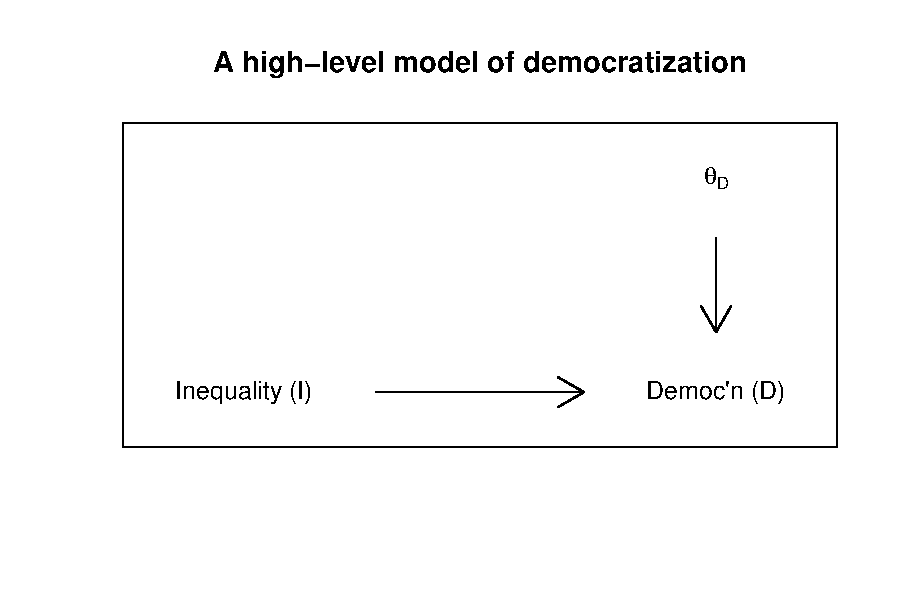
\includegraphics{ii_files/figure-latex/dagdemochigh-1} 

}

\caption{Simple democracy, inequality model}\label{fig:dagdemochigh}
\end{figure}

Nonetheless, we can increase the prospects for learning by \emph{theorizing} the relationship between inequality and democratization. Given causal logics and empirical findings in the existing literature, we can say more than is contained in Figure \ref{fig:dagdemochigh} about the possible structure of the causal linkages between inequality and democratization. And we can embed this prior knowledge of the possible causal relations in this domain in a lower-level model that is consistent with the high-level model that most simply represents our query.

If we were to seek to fully capture them, the models developed by Boix, Acemoglu and Robinson, and Ansell and Samuels would, each individually, suggest causal graphs with a large number of nodes and edges connecting them. Representing all variables and relationships jointly contained in these three models would take an extremely complex graph. Yet there is no need to go down to the lowest possible level---to generate the \emph{most} detailed graph---in order to increase our empirical leverage on the problem.

We represent in Figure \ref{fig:lowdem} one possible lower-level model consistent with our high-level model. Drawing on causal logics in the existing literature, we unpack the nodes in the high-level model in two ways:

\begin{enumerate}
\def\labelenumi{\arabic{enumi}.}
\item
  We interpose a mediator between inequality and democratization: mobilization (\(M\)) by economically disadvantaged groups expressing material grievances. \(M\) is a function of both \(I\) and of its own response-type variable, \(\theta^M\), which defines its response to \(I\). In inserting this mediator, we have extracted \(\theta^M\) from \(\theta^D\), pulling out that part of \(D\)'s response to \(I\) that depends on \(M\)'s response to \(I\).
\item
  We specify a second influence on democratization, international pressure (\(P\)). Like \(\theta^M\), \(P\) has also been extracted from \(\theta^D\); it represents that part of \(D\)'s response to \(I\) that is conditioned by international pressures.
\end{enumerate}

\begin{figure}

{\centering 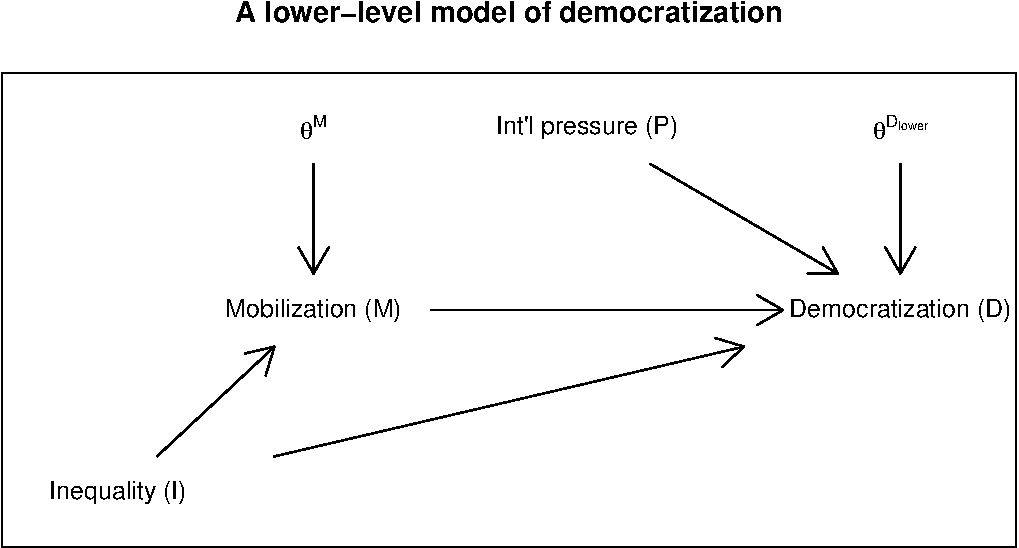
\includegraphics[width=.7\textwidth]{ii_files/figure-latex/lowdem-1} 

}

\caption{A lower-level model of democratization in which inequality may affect regime type both directly and through mobilization of the lower classes, and international pressure may also affect regime type.}\label{fig:lowdem}
\end{figure}

In representing the causal dependencies in this graph, we allow for inequality to have (in the language of mediation analysis) both an ``indirect'' effect on democratization via mobilization and a ``direct'' effect. The arrow running directly from \(I\) to \(D\) allows for effects of inequality on democratization beyond any effects running via mobilization of the poor, including effects that might run in the opposite direction. (For instance, it is possible that inequality has a positive effect on democratization via mobilization but a negative effect via any number of processes that are not explicitly specified in the model.) The graph also implies that there is no confounding: since there is no arrow running from another variable in the graph to \(I\), \(I\) is modeled as exogenous.

The lower-level graph thus has two exogenous, response-type nodes that will be relevant to assessing causal effects: \(\theta^M\) and \(\theta^{D_{lower}}\). \(\theta^M\), capturing \(I\)'s effect on \(M\), ranges across the usual four values for a single-cause, binary setup: \(\theta_{00}^M, \theta_{01}^M, \theta_{10}^M\), and \(\theta_{11}^M\).

\(\theta^{D_{lower}}\) is considerably more complicated, however, because this node represents \(D\)'s response to three causal variables: \(I\), \(M\), and \(P\). One way to put this is that the values of \(\theta^{D_{lower}}\) indicate how inequality's direct effect will depend on mobilization (and vice-versa), conditional on whether or not there is international pressure. We need more complex notation than that introduced in Chapter 5 in order to represent the possible response types here.

The result is \(2^8=256\) possible response types for \(D\). With 4 response types for \(M\), we thus have 1024 possible combinations of causal effects between named variables in the lower-level graph. How do these lower-level response types map onto the higher-level response types that are of interest? In other words, which combinations of lower-level types represent a positive, negative, or zero causal effect of inequality on democratization?

To define a causal effect of \(I\) in this setup, we need to define the ``joint effect'' of two variables as being the effect of changing both variables simultaneously (in the same direction, unless otherwise specified). Thus, the joint effect of \(I\) and \(M\) on \(D\) is positive if changing both \(I\) and \(M\) from \(0\) to \(1\) changes \(D\) from \(0\) to \(1\). We can likewise refer to the joint effect of an increase in one variable and a decrease in another. Given this definition, a positive causal effect of inequality on democratization emerges for any of the following three sets of lower-level response patterns:

\begin{enumerate}
\def\labelenumi{\arabic{enumi}.}
\item
  \textbf{Linked positive mediated effects.} \(I\) has a positive effect on \(M\); and \(I\) and \(M\) have a \emph{joint} positive effect on \(D\) when \(P\) takes on whatever value it takes on in the case.
\item
  \textbf{Linked negative mediated effects} \(I\) has a negative effect on \(M\); and \(I\) and \(M\) have a \emph{joint} negative effect on \(D\) when \(P\) takes on whatever value it takes on in the case.
\item
  \textbf{Positive direct effect} \(I\) has no effect on \(M\) and \(I\) has a positive effect on \(D\) at whatever value \(M\) is fixed at and whatever value \(P\) takes on in the case.
\end{enumerate}

If we start out with a case in which inequality is high and democratization has not occurred (or inequality is low and democratization \emph{has} occurred), we will be interested in the possibility of a negative causal effect. A negative causal effect of inequality on democratization emerges for any of the following three sets of lower-level response patterns:

\begin{enumerate}
\def\labelenumi{\arabic{enumi}.}
\setcounter{enumi}{3}
\item
  \textbf{Positive, then negative mediated effects} \(I\) has a positive effect on \(M\); and \(I\) and \(M\) have a \emph{joint} negative effect on \(D\) when \(P\) takes on whatever value it takes on in the case.
\item
  \textbf{Negative, then joint negative mediated effects} \(I\) has a negative effect on \(M\); and jointly increasing \(I\) while decreasing \(M\) generates a decrease in \(D\) when \(P\) takes on whatever value it takes on in the case.
\item
  \textbf{Negative direct effects} \(I\) has no effect on \(M\) and \(I\) has a negative effect on \(D\) at whatever value \(M\) is fixed at and whatever value \(P\) takes on in the case.
\end{enumerate}

Finally, all other response patterns yield \emph{no} effect of inequality on democratization.

Thus, for a case in which \(I=D=1\), our query amounts to assessing the probability that \(\theta^M\) and \(\theta^D_{lower}\) jointly take on values falling into conditions 1, 2, or 3. And for a case in which \(I \neq D\), where we entertain the possibility of a negative effect, our query is an assessment of the probability of conditions 4, 5, and 6.

\hypertarget{forming-priors}{%
\subsection{Forming Priors}\label{forming-priors}}

We now need to express prior beliefs about the probability distribution from which values of \(\theta^M\) and \(\theta^D_{lower}\) are drawn. We place structure on this problem by drawing a set of beliefs about the likelihood or monotonicity of effects and interactions among variables from the theories in Boix, Acemoglu and Robinson, and Ansell and Samuels. As a heuristic device, we weight more heavily those propositions that are more widely shared across the three works than those that are consistent with only one of the frameworks. We intend this part of the exercise to be merely illustrative of how one might go about forming priors from an existing base of knowledge; there are undoubtedly other ways in which one could do so from the inequality and democracy literature.

Specifically, the belief that we embed in our priors about \(\theta^M\) is:

\begin{itemize}
\tightlist
\item
  \textbf{Monotonicity of \(I\)'s effect on \(M\)}: In Acemoglu and Robinson, inequality should generally increase the chances of---and, in Boix, should never prevent---mobilization by the poor. Only in Ansell and Samuels' model does inequality have a partial downward effect on the poor's demand for democracy insofar as improved material welfare for the poor increases the chances of autocratic expropriation; and this effect is countervailed by the greater redistributive gains that the poor will enjoy under democracy as inequality rises.\footnote{In addition, as the industrial bourgeoisie become richer, which increases the Gini, this group faces a greater risk of autocratic expropriation. If we consider the rising bourgeosie's mobilization to be mobilization by a materially disadvantaged group, then this constitutes an additional positive effect of inequality on mobilization.} Consistent with the weight of prior theory on this effect, in our initial run of the analysis, we rule out negative effects of \(I\) on \(M\). We are indifferent in our priors between positive and null effects and between the two types of null effects (mobilization always occurring or never occurring, regardless of the level of inequality). We thus set our prior on \(\theta^M\) as: \(p(\theta^M=\theta^M_{10})=0.0\), \(p(\theta^M=\theta^M_{00})=0.25\), \(p(\theta^M=\theta^M_{11})=0.25\), and \(p(\theta^M=\theta^M_{01})=0.5\). We relax this monotonicity assumption, to account for the Ansell and Samuels logic, in a second run of the analysis.
\end{itemize}

For our prior on democracy's responses to inequality, mobilization, and international pressure (\(\theta^D_{lower}\)), we extract the following beliefs from the literature:

\begin{itemize}
\item
  \textbf{Monotonicity of direct \(I\) effect: no positive effect}: In none of the three theories does inequality promote democratization via a pathway \emph{other than} via the poor's rising demand for it. In all three theories, inequality has a distinct negative effect on democratization via an increase in the elite's expected losses under democracy and thus its willingness to repress. In Ansell and Samuels, the distribution of resources also affects the probability of success of rebellion; thus higher inequality also reduces the prospects for democratization by strengthening the elite's hold on power. We thus set a zero prior probability on all types in which \(I\)'s direct effect on \(D\) is positive for any value of \(P\).
\item
  \textbf{Monotonicity of \(M\)'s effect: no negative effect}: In none of the three theories does mobilization reduce the prospects of democratization. We thus set a zero probability on all types in which \(M\)'s effect on \(D\) is negative at any value of \(I\) or \(P\).
\item
  \textbf{Monotonicity of \(P\)'s effect: no negative effect}: While international pressures are only discussed in Haggard and Kaufman's study, none of the studies considers the possibility that international pressures to democratize might prevent democratization that would otherwise have occurred. We thus set a zero probability on all types in which \(P\)'s effect is negative at any value of \(I\) or \(M\).
\end{itemize}

In all, this reduces the number of nodal types for \(D\) from 256 to just 20.

For all remaining, allowable types, we set flat priors.

The remaining 20 allowable types can involve a rich range of interactions between international pressure, inequality, and mobilization, including::

\begin{enumerate}
\def\labelenumi{\arabic{enumi}.}
\item
  Types for which \(P\) has no moderating effect
\item
  Types for which \(P=1\) creates an ``opportunity'' for \(X\) to have an effect that it does not have at \(P=0\); at \(P=1\) and \(X=0\), \(D\) takes on the value it does when \(X=0\) and \(X\) has an effect, but does not take on this value when \(P=0\) and \(X=0\)
\item
  Types for which \(P=1\) is a causal ``complement'' to \(X\), allowing \(X\) to have an effect it did not have at \(P=0\); at \(P=1\) and \(X=1\), \(D\) takes on the value it does when \(X=1\) and \(X\) has an effect, but does not take on this value when \(P=0\) and \(X=1\)
\item
  Types for which \(P=1\) ``substitutes'' for \(X\), generating the outcome that \(X=1\) was necessary to generate at \(P=0\); at \(P=1\) and \(X=0\), \(D\) takes on the value it does when \(X=1\) and \(X\) has an effect, but does not take on this value when \(P=0\) and \(X=0\)
\item
  Types for which \(P\) ``eliminates'' \(X\)'s effect, preventing \(X=1\) from generating the outcome it generates when \(P=0\); at \(P=1\) and \(X=1\), \(D\) does not take on the value it does when \(X=1\) and \(X\) has an effect, but does take on this value when \(P=0\) and \(X=1\)
\end{enumerate}

Since \(P\) conditions the effect of \(I\), we must also establish a prior on the distribution of \(P\). In this analysis, we set the prior probability of \(P=1\) to 0.5, implying that before seeing the data we think that international pressures to democratize are present half the time.

\hypertarget{results}{%
\section{Results}\label{results}}

We can now choose nodes in addition to \(I\) and \(D\) to observe from the lower-level model. Recall that our query is about the joint values of \(\theta^M\) and \(\theta^{D_{lower}}\). By the logic \(d-\)separation, we can immediately see that both \(M\) and \(P\) may be informative about these nodes when \(D\) has already been observed. Conditional on \(D\), both \(M\) and \(P\) are \(d-\)connected to both \(\theta^M\) and \(\theta^{D_{lower}}\). Let us see what we learn, then, if we search for either mobilization of the lower classes or international pressure or both, and find either clue either present or absent.

We consider four distinct situations, corresponding to four possible combinations of inequality and democratization values that we might be starting with. In each situation, the nature of the query changes. Where we start with a case with low inequality and no democratization, asking if inequality caused the outcome is to ask if the lack of inequality caused the lack of democratization. Where we have high inequality and no democratization, we want to know if democratization was prevented by high inequality (as high inequality does in Boix's account). For cases in which democratization occurred, we want to know whether the lack or presence of inequality (whichever was the case) generated the democratization.

Inference is done by applying Bayes rule to the observed data given the priors. Different ``causal types'' are consistent or inconsistent with possible data observations. Conversely the observation of data lets us shift weight towards causal types that are consistent with the data and away from those that are not. As a simple illustration if we observe \(D=1\) then we would shift weight from types for which \(D\) is always 0, given the observed data, to types for which \(D\) can be 1 given the observed data.

\hypertarget{inferences-for-cases-with-observed-democratization}{%
\subsection{Inferences for cases with observed democratization}\label{inferences-for-cases-with-observed-democratization}}

We first turn to cases in which democratization has occurred---the category of cases that Haggard and Kaufman examine.

For these cases we use data from \citet{haggard2012inequality} to show the inferences we would draw using this procedure and the actual observations made for a set of 8 cases.

Haggard and Kaufman consider only cases that democratized, so all cases in this table have the value \(D=1\). We show here how confident we would be that the level inequality caused democratization if (a) we observed only the cause and effect (\(I\) and \(D\)); (b) we additionally observed either the level of mobilization by disadvantaged classes or the level of international pressure; and (c) if we observed both, in addition to \(I\) and \(D\). Note that countries labels are marked in the ``full data'' cells in the lower right quadrant, but their corresponding partial data cells can be read by moving to the left column or the top row (or to the top left cell for the case with no clue data).

In coding countries' level of inequality, we rely on Haggard and Kaufman's codings using the Gini coefficient from the Texas Inequality dataset. In selecting cases of democratization, we use the codings in \citet{cheibub2010democracy}, one of two measures used by Haggard and Kaufman. Our codings of the \(M\) and \(P\) clues come from close readings of the country-specific transition accounts in \citet{haggard2012distributive}, the publicly shared qualitative dataset associated with \citet{haggard2012inequality}. We code \(M\) as \(1\) where the transition account refers to anti-government or anti-regime political mobilization by economically disadvantaged groups, and as \(0\) otherwise. For \(P\), we code \(P=0\) if international pressures to democratize are not mentioned in the transition account. The main estimates refer to analyses with only qualitative, monotonicity restrictions on our priors. We also show in square brackets the estimates if we allow for a negative effect of inequality on mobilization but believe it to be relatively unlikely.

\hypertarget{i0-d1-low-inequality-democracies}{%
\subsubsection{\texorpdfstring{\(I=0, D=1\): Low inequality democracies}{I=0, D=1: Low inequality democracies}}\label{i0-d1-low-inequality-democracies}}

In a case that had low inequality and democratized, did low inequality cause democratization, as Boix's thesis would suggest? Looking at the first set of cases in Table \ref{tab:HK8cases1}, did Mexico, Albania, Taiwan, and Nicaragua democratize because they had relatively low inequality? Based only on observing the level of inequality and the outcome of democratization, we would place a 0 probability on inequality having been a cause. What can we learn, then, from our two clues?

We are looking here for a negative effect of \(I\) on \(D\), which in our model can only run via a direct effect, not through mobilization. Thus, the learning from \(M\) is limited for the same reason as in an \(I=1, D=0\) case. And \(M\) is modestly informative as a moderator for the same reasons and in the same direction, with observing mobilization generally reducing our confidence in inequality's negative effect relative to observing no mobilization. In our four cases, if we observe the level of mobilization, our confidence that inequality mattered goes up slightly (to 0) in Mexico and Taiwan, where mobilization did not occur, and goes down slightly in Albania and Nicaragua (to 0) where mobilization did occur.

\begin{table}

\caption{\label{tab:HK8cases1}Four cases with low inequality and  democratization. Question of interest: Was low inequality a cause of democracy? Table shows posterior beliefs for different data for four cases given information on $M$ or $P$. Data from Haggard and Kaufman (2012). Analyses here use priors assuming only monotonic effects.}
\centering
\resizebox{\linewidth}{!}{
\begin{tabular}[t]{lllllll}
\toprule
Case & M: Mobilization? & P: Pressure? & No clues & M only & P only & M and P\\
\midrule
\cellcolor{gray!6}{Mexico (2000)} & \cellcolor{gray!6}{0} & \cellcolor{gray!6}{0} & \cellcolor{gray!6}{0.438} & \cellcolor{gray!6}{0.475} & \cellcolor{gray!6}{0.615} & \cellcolor{gray!6}{0.667}\\
Taiwan (1996) & 0 & 1 & 0.438 & 0.475 & 0.34 & 0.393\\
\cellcolor{gray!6}{Albania (1991)} & \cellcolor{gray!6}{1} & \cellcolor{gray!6}{0} & \cellcolor{gray!6}{0.438} & \cellcolor{gray!6}{0.394} & \cellcolor{gray!6}{0.615} & \cellcolor{gray!6}{0.571}\\
Nicaragua (1984) & 1 & 1 & 0.438 & 0.394 & 0.34 & 0.263\\
\bottomrule
\end{tabular}}
\end{table}

Looking for the international pressure clue is, however, highly informative, though the effect runs in the opposite direction as in an \(I=1, D=0\) case. It is observing the absence of international pressure that makes us more confident in low inequality's effect. Since democratization \emph{did} occur, the presence of international pressure makes it less likely for low inequality to have generated the outcome since international pressure could have generated democratization by itself. Once we bring this second clue into the analysis, Mexico and Taiwan sharply part ways: seeing no international pressure in Mexico, we are now much more confident that inequality mattered for the Mexican transition (1); seeing international pressure in Taiwan, we are now substantially less confident that inequality mattered to the Taiwanese transition (0). Similarly, observing \(P\) sharply differentiates the Albanian and Nicaraguan cases: seeing no international pressure in the Albanian transition considerably boosts our confidence in inequality's causal role there (0), while observing international pressure in the Nicaraguan transition strongly undermines our belief in an inequality effect there (1).

\hypertarget{i1-d1-high-inequality-democracies}{%
\subsubsection{\texorpdfstring{\(I=1, D=1\): High inequality democracies}{I=1, D=1: High inequality democracies}}\label{i1-d1-high-inequality-democracies}}

Where we see both high inequality and democratization, the question is whether high inequality caused democratization via a positive effect. Considering the second set of cases in Table \ref{tab:HK8cases2}, did high inequality cause Mongolia, Sierra Leone, Paraguay, and Malawi to democratize?

Observing only the level of inequality and the democratization outcome, we would have fairly low confidence that inequality mattered, with a posterior on that effect of 1. Let us see what we can learn if we also observe the level of mobilization and international pressure.

As in an \(I=0, D=0\) case, \(M\) can now be highly informative since this positive effect has to run through mobilization. Here it is the observation of a lack of mobilization that is most telling: high inequality cannot have caused democratization, given our model, if inequality did not cause mobilization to occur. There is no point in looking for international pressure since doing so will have no effect on our beliefs. Thus, when we observe no mobilization by the lower classes in Mongolia and Paraguay, we can be certain (given our model) that high inequality did \emph{not} cause democratization in these cases. Moreover, this result does not change if we also go and look for international pressure: neither seeing pressure nor seeing its absence shifts our posterior away from 1.

\begin{table}

\caption{\label{tab:HK8cases2}Four cases with high inequality and  democratization. Question of interest: Was high inequality a cause of democratization? Table shows posterior beliefs for different data for 4 cases given information on $M$ or $P$. Data from Haggard and Kaufman (2012). Analyses here use priors assuming only monotonic effects.}
\centering
\resizebox{\linewidth}{!}{
\begin{tabular}[t]{lllllll}
\toprule
Case & M: Mobilization? & P: Pressure? & No clues & M only & P only & M and P\\
\midrule
\cellcolor{gray!6}{Mongolia (1990)} & \cellcolor{gray!6}{0} & \cellcolor{gray!6}{0} & \cellcolor{gray!6}{0.128} & \cellcolor{gray!6}{0} & \cellcolor{gray!6}{0.231} & \cellcolor{gray!6}{0}\\
Paraguay (1989) & 0 & 1 & 0.128 & 0 & 0.088 & 0\\
\cellcolor{gray!6}{Sierra Leone (1996)} & \cellcolor{gray!6}{1} & \cellcolor{gray!6}{0} & \cellcolor{gray!6}{0.128} & \cellcolor{gray!6}{0.15} & \cellcolor{gray!6}{0.231} & \cellcolor{gray!6}{0.25}\\
Malawi (1994) & 1 & 1 & 0.128 & 0.15 & 0.088 & 0.107\\
\bottomrule
\end{tabular}}
\end{table}

If we do see mobilization, on the other hand---as in Sierra Leone and Malawi---we are slightly more confident that high inequality was the cause of democratization (1). Moreover, if we first see \(M=1\), then observing international pressure can add much more information; and it substantially differentiates our conclusions about the causes of Sierra Leone's and Malawi's transitions. Just as in an \(I=0, D=1\) case, it is the absence of international pressure that leaves the most ``space'' for inequality to have generated the democratization outcome. When we see the absence of pressure in Sierra Leone, our confidence that high inequality was a cause of the transition increases to 0; seeing pressure present in Malawi reduces our confidence in inequality's effect to 1.

\hypertarget{cases-with-incomplete-data}{%
\subsection{Cases with incomplete data}\label{cases-with-incomplete-data}}

We next consider causal relations for cases that did not democratize. These cases are not included in \citet{haggard2012inequality} but our model nevertheless characterizes our beliefs for these cases also.

The results for cases that did not democratize (at the time in question) are presented in Table \ref{tab:Tapp1} and Table \ref{tab:Tapp2}. Each table shows, for one kind of case, our posterior beliefs on the causal responsibility of \(I\) for the outcome for different search strategies.

\hypertarget{i0-d0-non-democracy-with-low-inequality}{%
\subsubsection{\texorpdfstring{\(I=0, D=0\): Non democracy with low inequality}{I=0, D=0: Non democracy with low inequality}}\label{i0-d0-non-democracy-with-low-inequality}}

To begin with \(I=0, D=0\) cases, did the lack of inequality cause the lack of democratization (as, for instance, at the lefthand end of the Acemoglu and Robinson inverted \(U\)-curve)?

\begin{table}

\caption{\label{tab:Tapp1}No inequality and No democratization: Was no inequality a cause of no democratization? Analyses here use priors assuming only monotonic effects.}
\centering
\begin{tabular}[t]{lrrr}
\toprule
  & P & M & posterior\\
\midrule
\cellcolor{gray!6}{I0P0M0D0} & \cellcolor{gray!6}{0} & \cellcolor{gray!6}{0} & \cellcolor{gray!6}{0.107}\\
I0P1M0D0 & 1 & 0 & 0.250\\
\cellcolor{gray!6}{I0P0M1D0} & \cellcolor{gray!6}{0} & \cellcolor{gray!6}{1} & \cellcolor{gray!6}{0.000}\\
I0P1M1D0 & 1 & 1 & 0.000\\
\cellcolor{gray!6}{I0M0D0} & \cellcolor{gray!6}{} & \cellcolor{gray!6}{0} & \cellcolor{gray!6}{0.150}\\
\addlinespace
I0M1D0 &  & 1 & 0.000\\
\cellcolor{gray!6}{I0P0D0} & \cellcolor{gray!6}{0} & \cellcolor{gray!6}{} & \cellcolor{gray!6}{0.088}\\
I0P1D0 & 1 &  & 0.231\\
\cellcolor{gray!6}{I0D0} & \cellcolor{gray!6}{} & \cellcolor{gray!6}{} & \cellcolor{gray!6}{0.128}\\
\bottomrule
\end{tabular}
\end{table}

We start out, based on the \(I\) and \(D\) values and our model, believing that there is a 0.107 chance that low inequality prevented democratization. We then see that our beliefs shift most dramatically if we go looking for mobilization and find that it was present. The reason is that any positive effect of \(I\) on \(D\) has to run through the pathway mediated by \(M\) because we have excluded a positive direct effect of \(I\) on \(D\) in our priors. Moreover, since we do not allow \(I\) to have a negative effect on \(M\), observing \(M=1\) when \(I=0\) must mean that \(I\) has no effect on \(M\) on this case, and thus \(I\) cannot have a positive effect on \(D\) (regardless also of what we find if we look for \(P\)). If we do \emph{not} observe mobilization when we look for it, we now think it is somewhat more likely that \(I=0\) caused \(D=0\) since it is still possible that high inequality \emph{could} cause mobilization.

We also see that observing whether there is international pressure has a substantial effect on our beliefs. When we observe \(M=1\) (or don't look for \(M\) at all), the presence of international pressure increases the likelihood that low inequality prevented democratization. Intuitively, this is because international pressure, on average across types, has a positive effect on democratization; so pressure's presence creates a greater opportunity for low inequality to counteract international pressure's effect and prevent democratization from occurring that otherwise would have (if there had been high inequality and the resulting mobilization).

\hypertarget{i1-d0-non-democracy-with-high-inequality}{%
\subsubsection{\texorpdfstring{\(I=1, D=0\): Non democracy with high inequality}{I=1, D=0: Non democracy with high inequality}}\label{i1-d0-non-democracy-with-high-inequality}}

In cases with high inequality and no democratization, the question is whether high inequality prevented democratization via a negative effect, as theorized by Boix. That negative effect has to have operated via inequality's direct effect on democratization since our monotonicity restrictions allow only positive effects via mobilization. Here, the consequence of observing \(P\) is similar to what we see in the \(I=0, D=0\) case: seeing international pressure greatly increases our confidence that high inequality prevented democratization, while seeing no international pressure moderately reduces that confidence. There is, returning to the same intuition, more opportunity for high inequality to exert a negative effect on democratization when international pressures are present, pushing toward democratization.

\begin{table}

\caption{\label{tab:Tapp2}Inequality and No democratization: Was inequality a cause of no democratization? Analyses here use priors assuming only monotonic effects.}
\centering
\begin{tabular}[t]{lrrr}
\toprule
  & P & M & posterior\\
\midrule
\cellcolor{gray!6}{I1P0M0D0} & \cellcolor{gray!6}{0} & \cellcolor{gray!6}{0} & \cellcolor{gray!6}{0.263}\\
I1P1M0D0 & 1 & 0 & 0.571\\
\cellcolor{gray!6}{I1P0M1D0} & \cellcolor{gray!6}{0} & \cellcolor{gray!6}{1} & \cellcolor{gray!6}{0.393}\\
I1P1M1D0 & 1 & 1 & 0.667\\
\cellcolor{gray!6}{I1M0D0} & \cellcolor{gray!6}{} & \cellcolor{gray!6}{0} & \cellcolor{gray!6}{0.394}\\
\addlinespace
I1M1D0 &  & 1 & 0.475\\
\cellcolor{gray!6}{I1P0D0} & \cellcolor{gray!6}{0} & \cellcolor{gray!6}{} & \cellcolor{gray!6}{0.340}\\
I1P1D0 & 1 &  & 0.615\\
\cellcolor{gray!6}{I1D0} & \cellcolor{gray!6}{} & \cellcolor{gray!6}{} & \cellcolor{gray!6}{0.438}\\
\bottomrule
\end{tabular}
\end{table}

Here, however, looking for \(M\) has more modest effect than it does in an \(I=0, D=0\) case. This is because we learn less about the indirect pathway from \(I\) to \(D\) by observing \(M\): as we have said, we already know from seeing high inequality and no democratization (and under our monotonicity assumptions) that any effect could not have run through the presence or absence of mobilization.

However, \(M\) provides some information because it, like \(P\), acts as \emph{moderator} for \(I\)'s direct effect on \(D\) (since \(M\) is also pointing into \(D\)). As we know, learning about moderators tells us something about (a) the rules governing a case's response to its context (i.e., its response type) and (b) the context it is in. Thus, in the first instance, observing \(M\) together with \(I\) and \(D\) helps us eliminate types inconsistent with these three data points. For instance, if we see \(M=0\), then we eliminate any type in which \(D\) is 0, regardless of \(P\)'s value, when \(M=0\) and \(I=1\). Second, we learn from observing \(M\) about the value of \(M\) under which \(D\) will be responding to \(I\). Now, because \(M\) is itself potentially affected by \(I\), the learning here is somewhat complicated. What we learn most directly from observing \(M\) is \emph{the effect of \(I\) on \(M\)} in this case. If we observe \(M=1\), then we know that \(I\) has no effect on \(M\) in this case; whereas if we observe \(M=0\), \(I\) might or might not have a positive effect on \(M\). Learning about this \(I \rightarrow M\) effect then allows us to form a belief about how likely \(M\) would be to be 0 or 1 if \(I\) changed from \(0\) to \(1\); that is, it allows us to learn about the context under which \(D\) would be responding to this change in \(I\) (would mobilization be occurring or not)? This belief, in turn, allows us to form a belief about how \(D\) will respond to \(I\) given our posterior beliefs across the possible types that the case is.

The net effect, assuming that we have not observed \(P\), is a small upward effect in our confidence that inequality mattered if we see no mobilization, and a small downward effect if we see mobilization. Interestingly, if we \emph{do} observe \(P\), the effect of observing \(M\) reverses: observing mobilization increases our confidence in inequality's effect, while observing no mobilization reduces it.

\hypertarget{theory-dependence}{%
\section{Theory dependence}\label{theory-dependence}}

Haggard and Kaufman set out to use causal process observations to test inequality-based theories of democratization against the experiences of ``Third Wave'' democratizations. Their principal test is to examine whether they see evidence of distributive conflict in the process of democratization, defined largely as the presence or absence of mobilization prior to the transition. They secondarily look for other possible causes, specifically international pressure and splits in the elite.

In interpreting the evidence, Haggard and Kaufman generally treat the absence of mobilization as evidence against inequality-based theories of democratization as a whole (p.~7). They also see the \emph{presence} of distributive mobilization in cases with high inequality and democratization as evidence against the causal role of inequality (p.~7). These inferences, however, seem only loosely connected to the logic of the causal theories under examination. Haggard and Kaufman express concern that inequality-oriented arguments point to ``cross-cutting effects'' (p.~1) of inequality, but do not systematically work through the implications of these multiple pathways for empirical strategy. Our analysis suggests that a systematic engagement with the underlying models can shift that interpretation considerably. Under the model we have formulated, where inequality is \emph{high}, the absence of mobilization in a country that democratized is indeed damning to the notion that inequality mattered. However, where inequality is \emph{low}---precisely the situation in which Boix's theory predicts that we will see democratization---things are more complicated. If we assume that inequality cannot prevent mobilization, then observing no mobilization does not work against the claim that inequality mattered for the transition; indeed, it slightly supports it, at least given what we think is a plausible model-representation of arguments in the literature. Observing the absence of inequality in such a case, however, can undercut an inequality-based explanation if (and only if) we believe it is possible that inequality might prevent mobilization that would otherwise have occurred. Further, in cases with high inequality and democratization, it is the \emph{absence} of mobilization by the lower classes that would be least consistent with the claim that inequality mattered. Observing mobilization, in contrast, pushes in favor of an inequality-based explanation.

Moreover, it is striking that Haggard and Kaufman lean principally on a mediator clue, turning to evidence of international pressure and elite splits (moderators, or alternative causes) largely as secondary clues to identify ``ambiguous'' cases. As we have shown, under a plausible model given prior theory, it is the moderator clue that is likely to be much more informative.

Of course, the model that we have written down is only one possible interpretation of existing theoretical knowledge. It is very possible that Haggard and Kaufman and other scholars in this domain hold beliefs that diverge from those encoded in our working model. The larger point, however, is that our process tracing inferences will inevitably \emph{depend}---and could depend greatly---on our background knowledge of the domain under examination. Moreover, formalizing that knowledge as causal model can help ensure that we are taking that prior knowledge systematically into account---that the inferences we draw from new data are consistent with the knowledge that we bring to the table.

The analysis also has insights regarding case selection. Haggard and Kaufman justify their choice of only \(D=1\) cases as a strategy ``designed to test a particular theory and thus rests on identification of the causal mechanism leading to regime change'' (p.~4). Ultimately, however, the authors seem centrally concerned with assessing whether inequality, as opposed to something else, played a key causal role in generating the outcome. As the results above demonstrate, however, there is nothing special about the \(D=1\) cases in generating leverage on this question. The tables for \(D=0\) show that, given the model, the same clues can shift beliefs about as much for \(D=0\) as for \(D=1\) cases. We leave a more detailed discussion of this kind of issue in model-based case-selection for Chapter \ref{caseselection}.

Finally we emphasize that all of the inference in this chapter depends on a model that is constrained by theoretical insights but not one that is trained by data. Although we are able to make many inferences using this model, given the characteristics of a case of interest, we have no empirical grounds to justify these inferences. In Chapter \ref{mixingapp} we show how this model can be trained with broader data from multiple cases and in Chapter \ref{evaluation} we illustrate how the model itself can be put into question.

\hypertarget{mixing}{%
\chapter{Integrated inferences}\label{mixing}}

\begin{headerbox}
We extend the analysis of Chapter \ref{pt} to settings in which we can simultaneously learn from data on treatments and outcomes in many cases and causal process data for a subset of cases. In doing so we update our theory from cases and \emph{use} our updated theory to draw case-level inferences. While our process tracing was entirely theory-informed, mixed-data inference is also \emph{data}-informed.

\end{headerbox}

In this chapter we generalize the model developed in Chapter \ref{pt} to research situations in which we have data on multiple cases.

We start with a conceptual point: the structure introduced in Chapter 6 for single-case analysis can be used \emph{as is} for multi-case analysis. Thus, the conceptual work for mixed methods inference from models has been done already. Our goal for the rest of the chapter is thus more technical than conceptual---to show how to shift focus beyond sample level queries and to exploit assumptions regarding independence across cases to generate simpler models of causal processes that affect many units. As we do so, we provide microfoundations for the models in Chapter \ref{ptapp} (as with those in \citet{humphreys2015mixing}) with the probative value of clues derivable from a causal structure and data rather than provided directly by researchers.

\hypertarget{sample-inference}{%
\section{Sample inference}\label{sample-inference}}

Conceptualized correctly, there is no deep difference between the logic of inference used in single-case and in multi-case studies. This is not because any single ``case'' can be disaggregated into many ``cases,'' thereby allowing for large \(n\) analysis on small problems \citep{king1994designing}. Rather, the opposite: fundamentally, model-based inference always involves comparing \emph{a} pattern of data with the logic of the model. Studies with multiple cases can, in fact, be conceptualized as single-case studies: we always draw our inferences from a single \emph{collection} of clues, whether those clues have come from one or from many units.

In practice, when we move from a causal model with one observation to a causal model with multiple observations, we can use the structure we introduced in Chapter \ref{pt} but simply replace nodes that have a single value (i.e., scalars) with nodes containing multiple values (i.e., vectors) drawn from multiple cases. We then make inferences about causal relations between nodes from seeing the values of those nodes' (or other nodes') vectors.

To illustrate, consider the following situation. Suppose that our model includes a binary treatment \(X\) that is assigned to 1 with probability 0.5; an outcome, \(Y\); and a third ``clue'' variable, \(K\), all observable. We posit an unobserved variable \(\theta^Y\), representing \(Y\)'s nodal type, with \(\theta^Y\) taking on values in \(\{a,b,c,d\}\) with equal probability. (We interpret the types in \(\{a,b,c,d\}\) as defined in Section \ref{counterfactualmodel}.) In addition to pointing into \(Y\), moreover, \(\theta^Y\) affects \(K\). In particular, \(K=1\) whenever \(X\) has an effect on \(Y\), while \(K=1\) with a 50\% probability otherwise. In other words, our clue \(K\) is informative about \(\theta^Y\), a unit's nodal type for \(Y\). As familiar from Chapters \ref{pt} and \ref{ptapp}, when we observe \(K\) in a case we can update on causal effects within the case since that \(K\) value will have different likelihoods under different values of \(\theta^Y\).

So far, we have described the problem at the unit level. Let's now consider a two-case setup. We do this by exchanging scalar nodes for vectors:

\begin{itemize}
\tightlist
\item
  We have a treatment node, \(X\), that can take on one of four values, \((0,0), (0,1), (1,0), (1,1)\) with equal probability.
\item
  \(\theta^Y\) is now a vector with two elements that can take on one of 16 values \((a,a), (a,b),\dots (d,d)\) as determined by \(\lambda_\theta\). We might imagine a uniform distribution over these 16 elements.
\item
  \(Y\) is a vector that is generated by \(\theta^Y\) and \(X\) in the obvious way (e.g., \(X=(0,0), \theta^Y=(a,b)\) generates outcomes \(Y=(1,0)\))
\item
  The vector \(K\) has the same domain as \(X\) and \(Y\), and element \(K[j]=1\) if \(\theta^Y[j]=b\).
\end{itemize}

Now, consider a causal estimand. In a single-case setup, we might ask whether \(X\) has an effect on \(Y\) in the case. For a multi-case setup, we might ask what the Sample Average Treatment Effect, \(\tau\), is. Note a subtle difference in the nature of the answers we seek in these two situations. In the first (single-case) instance, our estimand is binary---of the form: ``is the case a \(b\) type?''---and our answer is a probability. In the multi-case estimation of the sample average treatment effect (``SATE''), our estimand is categorical and our answer is a probability distribution: we are asking ``what is the probability that \(\tau\) is 0?,'' ``what is the probability that \(\tau\) is .5?'', and so on.

While the estimand shifts, we can use the tools introduced for single-case process tracing in Chapters \ref{pt} and \ref{ptapp} to analyze this (superficially) multi-case study. To begin, our prior on the probability that \(\tau=1\) is the prior that \(X\) has a positive effect on \(Y\) in both cases, that is, that \(\theta^Y = (b,b)\): just 1 in 16.

Now, suppose that we observe that, for both units, \(X=1\) and \(Y=1\). This data pattern is consistent only with four possible \(\theta\) vectors: \((b,b), (d,d), (b, d), (d,b)\). Moreover each of these four is equally likely to produce the data pattern we see. So our belief that \(\tau=1\) now shifts from 1 in 16 to to 1 in 4. Next, suppose that we further observe the data pattern \(\mathbf K = (1,1)\). The probability of this pattern for \(\Theta\) vector \((b,b)\) (\(\tau = 1\)) is 1. And for the type vectors \((d,d), (b, d), (d,b)\), the probability of this \(\mathbf K\) pattern is \(.25, .5,\) and \(.5\), respectively. Applying Bayes' rule, our updated belief that \(\tau = 1\) is then \(1/(1 + .25 + .5 + .5) = 4/9\).

We can similarly figure out the posterior probability on any possible value of \(\tau\) and so build up a full posterior distribution. And we can do so given any \(\mathbf K\) pattern (i.e., \(\mathbf K\) realization) across the cases. Thus, if we observe the data pattern \(\mathbf K = (0,1)\), the probability of this pattern for type vector \((b,b)\) (\(\tau = 1\)) is 0. For the type vectors \((d,d), (b, d), (d,b)\) it is \(.25, 0, .5\), respectively. Table \ref{tab:ch9patterns} shows the posterior distribution over a set of discrete treatment effect values given different \(K\) patterns observed.

\begin{longtable}[]{@{}llllllll@{}}
\caption{\label{tab:ch9patterns}. Inferences of causal effects for a sample.}\tabularnewline
\toprule
\(X\) pattern & \(Y\) pattern & \(K\) pattern & \(\tau = -1\) & \(\tau = -.5\) & \(\tau = 0\) & \(\tau = .5\) & \(\tau = 1\) \\
\midrule
\endfirsthead
\toprule
\(X\) pattern & \(Y\) pattern & \(K\) pattern & \(\tau = -1\) & \(\tau = -.5\) & \(\tau = 0\) & \(\tau = .5\) & \(\tau = 1\) \\
\midrule
\endhead
(1,1) & (1,1) & (1,1) & 0 & 0 & 1/9 & 4/9 & 4/9 \\
(1,1) & (1,1) & (1,0) & 0 & 0 & 1/3 & 2/3 & 0 \\
(1,1) & (1,1) & (0,0) & 0 & 0 & 1 & 0 & 0 \\
\bottomrule
\end{longtable}

The conceptual point is that the general logic of inference with multiple units is the same as that with one unit. In both situations, we work out the likelihood of any given data \emph{pattern} for each possible set of values of model parameters and update our beliefs about those parameters. And, from our posterior distribution over model parameters (e.g., \(\Theta^Y\)), we then derive a posterior distribution over the possible answers to our query (e.g., values of \(\tau\)).\footnote{Representing node values in vector forms like this allows for vector-level mappings that imply more complex dependencies between units. For instance we might imagine instead that we observe \(K=1\) if and only if \(\theta^Y = (b,b)\), in which case observation of \(K\) lets us distinguish between \(\tau = 1\) and \(\tau = .5\) but not between \(\tau = .5\) and \(\tau = 0\).}

\hypertarget{general-queries}{%
\section{General queries}\label{general-queries}}

Although the core conceptual logic is the same for multi-case and single-case inference, going forward, we operationalize these problems somewhat differently.

For the remainder of this chapter, and for the rest of the book, when we focus on multi-case studies, we will set our sights primarily on models that describe general processes. Rather than seeking to understand the average effect in a set of cases, we seek to understand the causal relations that gave rise to the set of cases. From these we sometimes draw inferences to cases but in general our models will involve queries pitched in general terms.

There are two reasons for this. The first is that we are interested in learning across cases: To figure out how what we see in one case provides insight for what is happening in another. We do this by using data on some cases to update our beliefs about a general model that we think is of relevance for other cases. Thus we seek to learn about a general model. The second reason is more practical. If we can think of units as draws from a large population, and then invoke independence assumptions across types, then we can greatly reduce complexity by analyzing problems at the unit level rather than at the population level. In the 2-case example above, the vector \(\theta^Y\) could take on any of 16 values (\((a,a), (a,b),\dots (d,d)\)). At the case level, however, the node \(\theta^Y\) can take on only 4 values (\(\{a,b,c,d\}\)), yet we can learn about each case's \(\theta^Y\) value from data drawn from all the cases. Thinking about it this way simplifies the problem by greatly reducing the parameter space, but it is not free. It requires invoking the assumption that (potential) outcomes across units do not depend on each other. If we cannot stand by that assumption, then we will need to build independence failures into our models.

Taking this step, the procedure we now use in the mixed methods works as follows.

\hypertarget{set-up}{%
\subsection{Set up}\label{set-up}}

\begin{enumerate}
\def\labelenumi{\arabic{enumi}.}
\item
  \textbf{A DAG}. As for process tracing, we begin with a graphical causal model specifying possible causal linkages between nodes. Our ``chain'' model for instance has DAG: \(X \rightarrow M \rightarrow Y\).
\item
  \textbf{Nodal types}. Just as in process tracing, the DAG and variable ranges define the set of possible nodal types in the model---the possible ways in which each variable is assigned (if exogenous) or determined by its parents (if endogenous). For the \(X \rightarrow M \rightarrow Y\) model there are 2 types for \(\theta^X\), 4 for \(\theta^M\), and 4 for \(\theta^Y\).
\item
  \textbf{Causal types}. A full set of nodal types gives rise to a full set of causal types, encompassing all possible combinations of nodal types across all nodes in the model. We let \(\theta\) denote an arbitrary causal type. For a \(X \rightarrow M \rightarrow Y\) model, one possible causal type would be \(\theta = (\theta^X_1, \theta^M_{01}, \theta^M_{01})\).
\item
  \textbf{Parameters.} As before, we use \(\lambda^V\) to denote the probabilities of \(\theta^V\) for a given node, \(V\). Recall that in process tracing, we sought to learn about \(\theta\) and our priors were given by \(\lambda\). When we shift to multi-case inference, \(\lambda\) becomes the parameter that we want to learn about: we seek to learn about the probability of different types arising in a population (or the \emph{shares} of types in a large population).
\item
  \textbf{Priors}. In the process tracing setup, we treat \(\lambda\) as given: we do not seek to learn about \(\lambda\), and uncertainty over \(\lambda\) plays no role. When we get to observe data on multiple cases, however, we have the opportunity to learn \emph{both} about the cases at hand \emph{and} about the population. Moreover, our level of uncertainty about population-level parameters will shape our inferences. We thus want our parameters (the \(\lambda\)'s) to be drawn from a prior \emph{distribution} --- a distribution that expresses our uncertainty and over which we can update once we see the data. While different distributions may be appropriate to the task in general, uncertainty over proportions (of cases, events, etc.) falling into a set of discrete categories is usefully described by a Dirichlet distribution, as discussed in Chapter \ref{bayeschapter}. Recall that the parameters of a Dirichlet distribution (the \(\alpha\)'s) can be thought of as conveying both the relative expected proportions in each category and our degree of uncertainty.
\end{enumerate}

\begin{figure}

{\centering 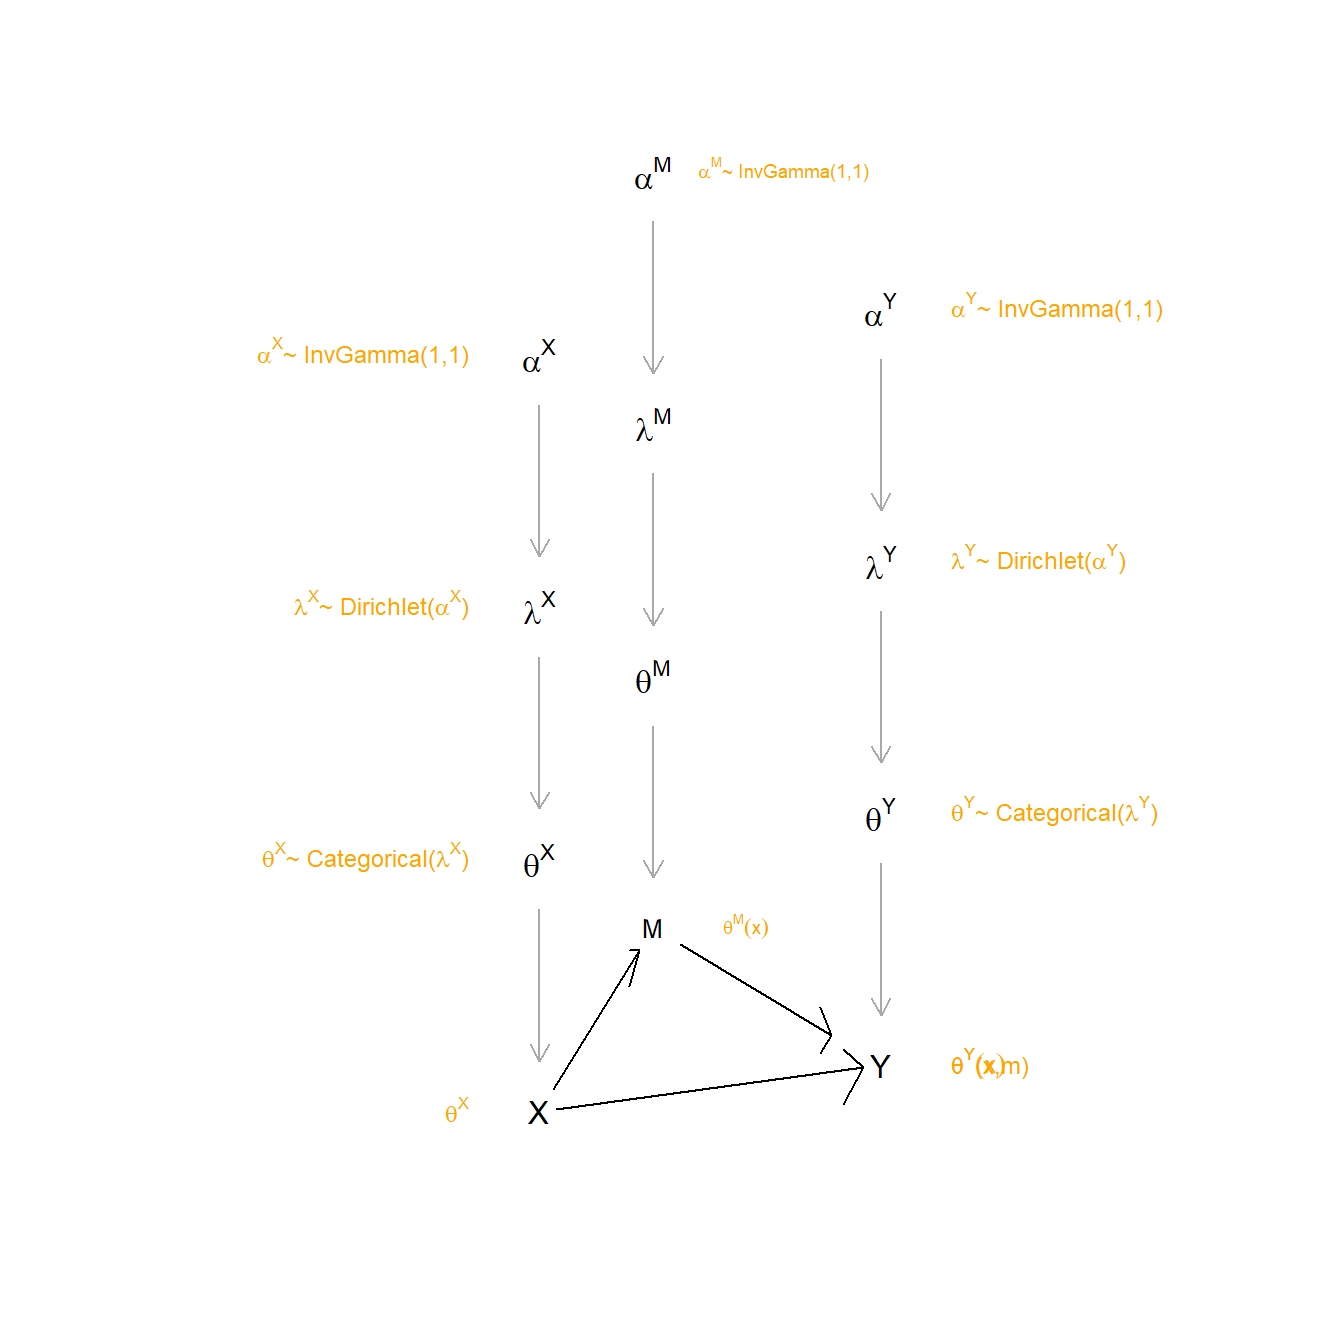
\includegraphics[width=1\linewidth]{ii_files/figure-latex/dag3d-1} 

}

\caption{Types, parameters, and priors}\label{fig:dag3d}
\end{figure}

\hypertarget{inference}{%
\subsection{Inference}\label{inference}}

Inference then works by figuring out the probability of the data given different possible parameter vectors, \(\lambda\)s, and then applying Bayes' rule. In practice we proceed as follows.

\textbf{Distributions over causal types.} We first need characterize our beliefs about causal types given any possible parameter vector \(\lambda\). Imagine a draw of one possible value of \(\lambda\) from the prior. This \(\lambda\) vector implies a set of nodal type shares for all nodes. That set of nodal type shares implies, in turn, a distribution over \emph{causal} types (\(\theta\)). For instance, the probability of causal type \(\theta = (\theta^X_1, \theta^Y_{01}, \theta^M_{01})\) is simply \(p(\theta|\lambda)=\lambda^X_1\lambda^M_{01}\lambda^Y_{01}\). More generally:

\[p(\theta|\lambda) = \prod_{k,v:\theta^v_k\in\theta}\lambda^v_k\]

\textbf{Event probabilities}. Each causal type in turn implies a single data realization, or data type. For instance \(\theta = (\theta^X_1, \theta^M_{01}, \theta^Y_{01})\) implies data \(X=1, M=1, Y=1\). Let \(D(\theta)\) denote the data type implied by causal type \(\theta\). A single data type, however, may be implied by multiple causal types. We use \(\Theta(d)\) to denote the set of causal types that imply a given data type:

\[\Theta(d) : \{\theta| D(\theta) = d \}\]

The probability of a given data type \(d\), is then:

\[w_d = \sum_{\theta \in \Theta(d)}p(\theta|\lambda)\]

And we use \(\mathbf w\) to denote the vector of event probabilities over all data types.

To illustrate, a data type \(d = (X=1, M =1, Y=1)\) is consistent with four different causal types in the \(X\rightarrow M\rightarrow Y\) model: \(\Theta(d) = \{(\theta^X_0, \theta^M_{01}, \theta^Y_{01}), (\theta^X_0, \theta^M_{11}, \theta^Y_{01}), (\theta^X_0, \theta^M_{01}, \theta^Y_{11}), (\theta^X_0, \theta^M_{11}, \theta^Y_{11})\}\). The probability of the data type is then calculated by summing up the probabilities of each causal type that implies the event: \(w_{111}:=\lambda^X_1(\lambda^M_{01} + \lambda^M_{11}))(\lambda^Y_{01} + \lambda^Y_{11})\).

In practice, calculating the full \(\mathbf w\) vector is made easier by the construction of a ``parameter matrix'' and an ``ambiguity matrix'', just as for process tracing, that tells us which causal types are consistent with a particular data type.

We use Tables \ref{tab:ambigmatrixmix} and \ref{tab:parammmatrixmix} to illustrate how to calculate the event probability for each data type for a given parameter vector \(\lambda\). Starting with data type \(X=0, Y=0\) (first column of the ambiguity matrix), we see that the consistent causal types are (\(\theta^X_0, \theta^Y_{00}\)) and (\(\theta^X_0, \theta^Y_{01}\)), in rows 1 and 4. We then turn to columns 1 and 4 of the parameter matrix to read off the probability of each of these causal types---in each case given by the probability of the nodal types that it is formed out of. This gives \(.4 \times .3\) and \(.4\times .2\) giving a total probability of \(0.2\) for the \(X=0, Y=0\) event. All four event probabilities, for the four data types, are then calculated in the same way.

In practice we do this all using matrix operations.

\begin{table}

\caption{\label{tab:ambigmatrixmix}An ambiguity matrix for a simple $X \rightarrow Y$ model (with no unobserved confounding). Rows are causal types, columns are data types.}
\centering
\begin{tabular}[t]{lrrrr}
\toprule
  & X0Y0 & X1Y0 & X0Y1 & X1Y1\\
\midrule
\cellcolor{gray!6}{X0Y00} & \cellcolor{gray!6}{1} & \cellcolor{gray!6}{0} & \cellcolor{gray!6}{0} & \cellcolor{gray!6}{0}\\
X1Y00 & 0 & 1 & 0 & 0\\
\cellcolor{gray!6}{X0Y10} & \cellcolor{gray!6}{0} & \cellcolor{gray!6}{0} & \cellcolor{gray!6}{1} & \cellcolor{gray!6}{0}\\
X1Y10 & 0 & 1 & 0 & 0\\
\cellcolor{gray!6}{X0Y01} & \cellcolor{gray!6}{1} & \cellcolor{gray!6}{0} & \cellcolor{gray!6}{0} & \cellcolor{gray!6}{0}\\
\addlinespace
X1Y01 & 0 & 0 & 0 & 1\\
\cellcolor{gray!6}{X0Y11} & \cellcolor{gray!6}{0} & \cellcolor{gray!6}{0} & \cellcolor{gray!6}{1} & \cellcolor{gray!6}{0}\\
X1Y11 & 0 & 0 & 0 & 1\\
\bottomrule
\end{tabular}
\end{table}

\begin{longtable}[]{@{}lrrrrrrrrr@{}}
\caption{\label{tab:parammmatrixmix}A parameter matrix for a simple \(X \rightarrow Y\) model (with no unobserved confounding), indicating a single draw of \(\lambda\) values from the prior distribution.}\tabularnewline
\toprule
& X0.Y00 & X1.Y00 & X0.Y10 & X1.Y10 & X0.Y01 & X1.Y01 & X0.Y11 & X1.Y11 & \(\lambda\) \\
\midrule
\endfirsthead
\toprule
& X0.Y00 & X1.Y00 & X0.Y10 & X1.Y10 & X0.Y01 & X1.Y01 & X0.Y11 & X1.Y11 & \(\lambda\) \\
\midrule
\endhead
X.0 & 1 & 0 & 1 & 0 & 1 & 0 & 1 & 0 & 0.4 \\
X.1 & 0 & 1 & 0 & 1 & 0 & 1 & 0 & 1 & 0.6 \\
Y.00 & 1 & 1 & 0 & 0 & 0 & 0 & 0 & 0 & 0.3 \\
Y.10 & 0 & 0 & 1 & 1 & 0 & 0 & 0 & 0 & 0.2 \\
Y.01 & 0 & 0 & 0 & 0 & 1 & 1 & 0 & 0 & 0.2 \\
Y.11 & 0 & 0 & 0 & 0 & 0 & 0 & 1 & 1 & 0.3 \\
\bottomrule
\end{longtable}

\textbf{Likelihood}. Now that we know the probability of observing each data pattern in a \emph{single} case given \(\lambda\), we can use these event probabilities to aggregate up to the likelihood of observing a data pattern across multiple cases (given \(\lambda\)). For this aggregation, we make use of an independence assumption: that each unit is independently drawn from a common distribution. Doing so lets us move from a categorical distribution that gives the probability that a single case has a particular data type to a \emph{multinomial} distribution that gives the probability of seeing an arbitrary data pattern across any number of cases.

Specifically, with discrete variables, we can think of a given multiple-case data pattern simply as a set of counts across categories. For, say, \(X, Y\) data, we will observe a certain number of \(X=0, Y=0\) cases (which we notate as \(n_{00}\)), a certain number of \(X=1, Y=0\) cases (\(n_{10}\)), a certain number of \(X=0, Y=1\) cases (\(n_{01}\)), and a certain number of \(X=1, Y=1\) cases (\(n_{11}\)). A data pattern, given a particular set of variables observed (a search strategy), thus has a multinomial distribution. The likelihood of a data pattern under a given search strategy, in turn, takes the form of a multinomial distribution conditional on the number of cases observed, \(n\), and the probability of each data type, given a \(\lambda\) draw. More formally, we write:

\[d \sim \text{Multinomial}(n, w(\lambda))\]

To illustrate, assume now that we have a 3-node model, with \(X, Y\), and \(M\) all binary. Let \(\mathbf n_{XYM}\) denote an 8-element vector recording the number of cases in a sample displaying each possible combination of \(X,Y,M\) data, thus: \(\mathbf D= \mathbf n_{XYM}:=(n_{000},n_{001},n_{100},\dots ,n_{111})\). The elements of \(\mathbf n_{XYM}\) sum to \(n\), the total number of cases studied. Likewise, let the event probabilities for data types given \(\lambda\) be registered in a vector, \(\mathbf w_{XYM}=(w_{000},w_{001},w_{100},\dots ,w_{111})\). The likelihood of a data pattern, \(\mathbf D\) is then:

\[
p(d|\lambda) = 
  \text{Multinom}\left(n_{XYM}|\sum n_{XYM}, w_{XYM}(\lambda)\right)  \\
\]
In other words, the likelihood of observing a particular data pattern given \(\lambda\) is given by the corresponding value of the multinomial distribution given the data probabilities.

\begin{enumerate}
\def\labelenumi{\arabic{enumi}.}
\setcounter{enumi}{3}
\tightlist
\item
  \textbf{Estimation}. We now have all the components for updating on \(\lambda\). Applying Bayes rule (see Chapter \ref{bayeschapter}), we have:
\end{enumerate}

\[p(\lambda | d) = \frac{p(d | \lambda)p(\lambda)}{\int_{\lambda'}{p(d | \lambda')p(\lambda')}}\]
In the \texttt{CausalQueries} package this updating is implemented in \texttt{stan}, and the result of the updating is a dataframe that contains a collection of draws from the posterior distribution for \(\lambda\). Table \ref{tab:posteriortable} illustrates what such a dataframe might look like for an \(X\rightarrow M \rightarrow Y\) model. Each row represents a single draw from \(p(\lambda|d)\). The 10 columns represent shares for each of the 10 nodal types in the model, under each \(\lambda\) draw.

\begin{table}

\caption{\label{tab:posteriortable}An illustration of a posterior distribution for a $X \rightarrow M \rightarrow Y$ model. Each row is a draw from $p(\lambda|d))$. Such a posterior would typically have thousands of rows and capture the full joint posterior distribution over all parameters.}
\centering
\begin{tabular}[t]{rrrrrrrrrr}
\toprule
X.0 & X.1 & M.00 & M.10 & M.01 & M.11 & Y.00 & Y.10 & Y.01 & Y.11\\
\midrule
\cellcolor{gray!6}{0.47} & \cellcolor{gray!6}{0.53} & \cellcolor{gray!6}{0.21} & \cellcolor{gray!6}{0.07} & \cellcolor{gray!6}{0.17} & \cellcolor{gray!6}{0.55} & \cellcolor{gray!6}{0.20} & \cellcolor{gray!6}{0.23} & \cellcolor{gray!6}{0.15} & \cellcolor{gray!6}{0.41}\\
0.68 & 0.32 & 0.02 & 0.41 & 0.38 & 0.19 & 0.12 & 0.20 & 0.07 & 0.61\\
\cellcolor{gray!6}{0.33} & \cellcolor{gray!6}{0.67} & \cellcolor{gray!6}{0.16} & \cellcolor{gray!6}{0.45} & \cellcolor{gray!6}{0.27} & \cellcolor{gray!6}{0.12} & \cellcolor{gray!6}{0.08} & \cellcolor{gray!6}{0.02} & \cellcolor{gray!6}{0.81} & \cellcolor{gray!6}{0.09}\\
0.68 & 0.32 & 0.15 & 0.10 & 0.70 & 0.05 & 0.03 & 0.07 & 0.00 & 0.90\\
\cellcolor{gray!6}{0.17} & \cellcolor{gray!6}{0.83} & \cellcolor{gray!6}{0.02} & \cellcolor{gray!6}{0.11} & \cellcolor{gray!6}{0.64} & \cellcolor{gray!6}{0.22} & \cellcolor{gray!6}{0.44} & \cellcolor{gray!6}{0.06} & \cellcolor{gray!6}{0.30} & \cellcolor{gray!6}{0.20}\\
\addlinespace
0.83 & 0.17 & 0.16 & 0.08 & 0.02 & 0.73 & 0.49 & 0.28 & 0.12 & 0.11\\
\bottomrule
\end{tabular}
\end{table}

\begin{enumerate}
\def\labelenumi{\arabic{enumi}.}
\setcounter{enumi}{4}
\tightlist
\item
  \textbf{Querying}.
\end{enumerate}

Once we have generated a posterior distribution for \(\lambda\), we can then query that distribution. The simplest queries relate to values of \(\lambda\). For instance, if we are interested in the probability that \(M\) has a positive effect on \(Y\), given an updated \(X \rightarrow M \rightarrow Y\) model, we want to know about the distribution of \(\lambda^M_{01}\). This distribution can be read directly from column 9 (\(Y01\)) of Table \ref{tab:posteriortable}. More complex queries can all be described as summaries of combinations of these columns. For instance, the query, ``What is the average effect of \(M\) on \(Y\)'' is a question about the distribution of \(\lambda^M_{01} - \lambda^M_{10}\), which is given by the difference between columns 9 and 8 of the table. Still more complex queries may require keeping some nodes constant while varying others, yet all of these can be calculated as summaries of the combinations of columns of the posterior distribution, following the rules described in Chapter \ref{questions}.

Table \ref{tab:chainillustration} shows examples of a full mapping from data to posteriors. We begin with a simple chain model of the form \(X\rightarrow M \rightarrow Y\) with flat priors over nodal types and report inferences on a set of queries (columns) for difference data types (rows).

\begin{longtable}[]{@{}lrrrrrrrr@{}}
\caption{\label{tab:chainillustration}Inferences on a chain model given different amounts of data (all on the diagonal, with X=0, Y=0 or X=1, Y=1). Columns 1-4 are shares of a, b, c, d causal types (as described in Chapter 2); columns 5 - 8 show \(\tau_{ij}\)---average effects of \(i\) on \(j\); the last column shows the probability of causation: the probability that \(X\) caused \(Y\) in a \(X=Y=1\) case.}\tabularnewline
\toprule
Data & a & b & c & d & \(\tau_{XM}\) & \(\tau_{MY}\) & \(\tau_{XY}\) & PC \\
\midrule
\endfirsthead
\toprule
Data & a & b & c & d & \(\tau_{XM}\) & \(\tau_{MY}\) & \(\tau_{XY}\) & PC \\
\midrule
\endhead
No data & 0.13 & 0.13 & 0.37 & 0.38 & 0.00 & -0.01 & 0.00 & 0.27 \\
2 cases X, Y data only & 0.12 & 0.14 & 0.37 & 0.37 & 0.00 & 0.00 & 0.02 & 0.29 \\
2 cases, X, M, Y data & 0.12 & 0.16 & 0.36 & 0.36 & 0.20 & 0.20 & 0.04 & 0.32 \\
10 cases: X, Y data only & 0.11 & 0.27 & 0.31 & 0.31 & 0.00 & 0.00 & 0.17 & 0.45 \\
10 cases: X, M, Y data & 0.09 & 0.44 & 0.23 & 0.23 & 0.59 & 0.59 & 0.35 & 0.66 \\
\bottomrule
\end{longtable}

\hypertarget{wrinkles}{%
\subsection{Wrinkles}\label{wrinkles}}

The procedure we described works in the same way for a very wide class of causal models. More attention is needed for special cases in which there is confounding, complex sampling, or sample estimands.

\hypertarget{unobserved-confounding.}{%
\subsubsection{Unobserved confounding.}\label{unobserved-confounding.}}

When there is unobserved confounding, we need parameter sets that allow for a joint distribution over nodal types. Unobserved confounding, put simply, means that there is confounding across nodes that is not captured by nodes and edges represented on the DAG. More formally, in the absence of unobserved confounding, we can treat the distribution of nodal types for a given node as independent of the distribution of nodal types for every other node. Unobserved confounding means that we believe that nodal types may be correlated across nodes. Thus, for instance, we might believe that those units assigned to \(M=1\) have different potential outcomes for \(Y\) than those assigned to \(M=0\) -- i.e., that the probability of \(M=1\) is correlated with whether or not \(M\) has an effect on \(Y\). To allow for such a correlation, we have to allow \(\theta^M\) and \(\theta^Y\) to have a joint distribution. There are different ways to do this in practice, but a simple approach is to split the parameter set corresponding to the \(Y\) node into two: we specify one distribution for \(\theta^Y\) when \(M=0\) and a separate distribution for \(\theta^Y\) when \(M=1\). For each of these parameter sets, we specify two \(\alpha\) parameters representing our priors. We can draw \(\lambda\) values for these conditional nodal types from the resulting Dirichlet distributions, as above, and can then calculate causal type probabilities in the usual way. Note that if we do this in an \(X \rightarrow M \rightarrow Y\) model, we have one 2-dimensional Dirichlet distribution corresponding to \(X\), one 4-dimensional Dirichlet distribution corresponding to \(M\), and two 4 dimensional distributions corresponding to \(Y\). In all, with 1+3+3+3 degrees of freedom: exactly the number needed to represent a joint distribution over all \(\theta^X, \theta^M, \theta^Y\) combinations.

In the figure below we represent this confounding by indicating parameters values \(\lambda_{MY}\) that determine the joint distribution over \(\theta_M\) and \(\theta_Y\).

\begin{figure}

{\centering 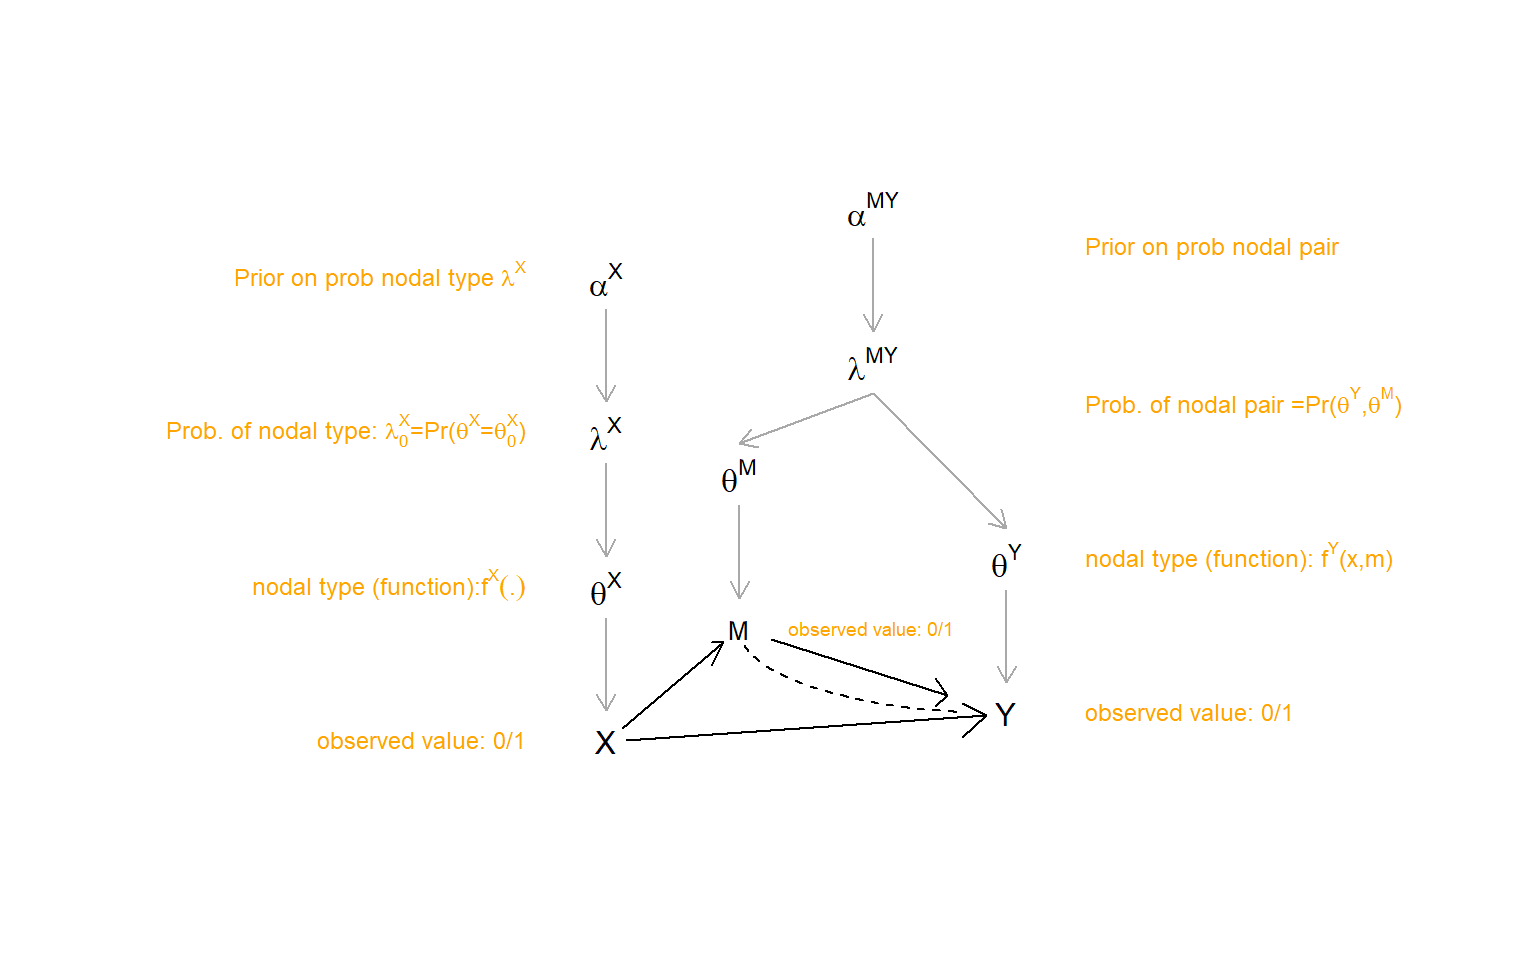
\includegraphics[width=0.95\linewidth]{ii_files/figure-latex/dag3d2-1} 

}

\caption{Types, parameters, and priors, with confounding}\label{fig:dag3d2}
\end{figure}

\hypertarget{sampling-and-the-likelihood-principle}{%
\subsubsection{Sampling and the likelihood principle}\label{sampling-and-the-likelihood-principle}}

In constructing a likelihood function, we sometimes need to take the sampling strategy into account. Sometimes however we can ignore the sampling procedure if we can invoke the ``likelihood principle''---the principle that the relevant information for inference is contained in the likelihood.

To see the likelihood principle in operation, consider the following \emph{conditional} data strategy: we collect data on \(X\) and \(Y\) in 2 cases, and we then measure \(M\) in any case in which we observe \(X=1, Y=1\).

We draw data and end up with one case with \(X=Y=0\) (\(M\) not observed) and one case with \(X=1, M=0, Y=1\) (\(M\) measured, following the strategy).

One way to think of the event probabilities is to think of a set of 5 possible events, as described in table below:

\begin{longtable}[]{@{}
  >{\raggedright\arraybackslash}p{(\columnwidth - 2\tabcolsep) * \real{0.26}}
  >{\raggedright\arraybackslash}p{(\columnwidth - 2\tabcolsep) * \real{0.74}}@{}}
\toprule
data type: & prob: \\
\midrule
\endhead
\(X1M0Y1\) & \(\lambda^X_1(\lambda^M_{00}+\lambda^M_{10})(\lambda^Y_{11}+\lambda^Y_{10})\) \\
\(X1M1Y1\) & \(\lambda^X_1(\lambda^M_{11}+\lambda^M_{01})(\lambda^Y_{11}+\lambda^Y_{01})\) \\
\(X0Y0\) & \(\lambda^X_0(\lambda^M_{00}+\lambda^M_{01})(\lambda^Y_{00}+\lambda^Y_{01}) + \lambda^X_0(\lambda^M_{10}+\lambda^M_{11})(\lambda^Y_{00}+\lambda^Y_{10})\) \\
\(X0Y1\) & \(\lambda^X_0(\lambda^M_{00}+\lambda^M_{01})(\lambda^Y_{10}+\lambda^Y_{11}) + \lambda^X_0(\lambda^M_{10}+\lambda^M_{11})(\lambda^Y_{01}+\lambda^Y_{11})\) \\
\(X1Y0\) & \(\lambda^X_1(\lambda^M_{00}+\lambda^M_{10})(\lambda^Y_{00}+\lambda^Y_{01}) + \lambda^X_1(\lambda^M_{01}+\lambda^M_{11})(\lambda^Y_{00}+\lambda^Y_{10})\) \\
\bottomrule
\end{longtable}

In this conditional strategy view (draw \(X\), \(Y\) first and then draw \(M\) based on what you find) we have

\begin{itemize}
\tightlist
\item
  \(2P(X=0, Y=0)P(X=1, Y=1)P(M=0 | X=1, Y=1)\)
\end{itemize}

The two observations could however also be thought of as coming from a simple multinomial draw from the five event types in the table above. Call this the single multinomial view.

In the single multinomial view we have the probability of seeing data with \(X=Y=0\) in one case and \(X=1, M=0, Y=1\) in another is:

\begin{itemize}
\tightlist
\item
  \(2P(X=0, Y=0)P(X=1, M=0, Y=1)\)
\end{itemize}

But since \(P(X=1, Y=1)P(M=0 | X=1, Y=1) = P(M=0 | X=1, Y=1)\) these two expressions are the same ``up to a constant'' and so the inferences we make will be the same under both views.

Consider now a third strategy in which rather than conditioning \(X=Y=1\) to examine \(M\), one of the two cases were chosen at random to observe \(M\) and it just so happened to be a case with \(X=Y=1\). Or another strategy in which for each data point researchers randomly determined whether to gather data on \(M\) or not. In all of these cases the probability of observing the data we do in fact observe has the same basic form, albeit with possibly different constants.

In other words, these details of sampling can be ignored.

Other sampling procedures do have to be taken into account however, in particular, sampling---or more generally missingness---that is related to potential outcomes. As the simplest illustration consider a model in which \(X \rightarrow Y\), but data is only recorded in cases in which \(Y=1\). Then a naive implementation of our procedure would infer that \(Y=1\) regardless of \(X\) and so \(X\) has no effect on \(Y\). The problem here is that the likelihood is not taking account of the process through which cases enter our data. In this case the correct likelihood would make use of event probabilities of the form:

\[x_d = \sum_{\theta \in \Theta(d)}p(\theta|\lambda)\]
Let \(D^*\) denote the set of data types involving \(Y=1\). Then:
\[w_d =  \left\{ \begin{array}{cc}
0 & \text{if } d\not\in D^* \\
\frac{x_d}{\sum_{d'\in D^*}x_{d'}} & \text{otherwise} \end{array} \right.\]

While this kind of sampling can be handled relatively easily (it is implemented also in the \texttt{CausalQueries} package) the general principle holds that sampling (missingness) that is related to potential outcomes is a part of the data generating process and needs to be taken into account in the likelihood. For strategies to address non random sampling by blocking, see \citet{bareinboim2016causal}.

\hypertarget{case-inference-following-population-updating}{%
\subsubsection{Case inference following population updating}\label{case-inference-following-population-updating}}

We are often in situations in which we observe patterns in \(n\) units and then seek to make an inference about one or more of the \(n\) cases conditional on \emph{both} the case level data and the broader patterns in the full data.

Divide cases into set \(S^0, S^1\) where \(S^0\) is the set for which we wish to make case level inferences and \(S^1\) is the collection of other cases for which we have data.

In such cases should one use the data from \(S^0\) when updating on population estimands or rather update using \(S^1\) only and use information on \(S^1\) for the case level inferences only?

The surprising answer is that it is possible to do both, though exactly how queries are calculated depends on the method used.

Let \(\Lambda\) denote a collection of possible population parameters with typical element \(\lambda^i\). Let \(p\) denote a distribution over \(\Lambda\) (after updating on data from set \(S^1\)), with typical element \(\lambda^i\). Let \(X\) denote possible data for cases in \(S^0\) with realization \(x\).

Let \(d^i\) denote the probability of observing data \(X = x\) for a case (or set of cases) given \(\lambda^i\).

Let \(\tau^{|x}\) denote a query of interest---where the query is conditional in the sense that it relates to cases with data \(x\). An example might be: what is the effect of \(X\) on \(Y\) in a case in which \(M=1\) and \(Y=1\). Let \(q^i_j\) denote the probability that \(\tau^{|x} = \tau_j^{|x}\) when \(\lambda = \lambda^i\) for a case with data \(X=x\). Note \(q^i_j\) can be written \(z^i/d^i\) where \(z^i_j = \Pr(\tau^{|x} = \tau^{|x}_j, X=x | \lambda^i)\).

To illustrate, say in an \(X\rightarrow Y\) model we were interested in the effect of \(X\) on \(Y\) in a case with \(X=1, Y=1\). Then \(d^i = (\lambda^i)^X_1((\lambda^i)^Y_{01} + (\lambda^i)^Y_{11})\) is the probability of observing (\((X=1, Y=1)\). Then for query \(\tau^{|x}_j = 1\) (did \(X\) cause \(Y\)) we have \(z^i_j = (\lambda^i)^X_1((\lambda^i)^Y_{01})\), and so the probability of this query for this case given \(\lambda^i\) is: \(q^i_j = \frac{(\lambda^i)^Y_{01}}{(\lambda^i)^Y_{01} + (\lambda^i)^Y_{11}}\)

The posterior on \(\tau^{S^0}\) for the cases in \(S^0\) that provide data \(x\), is then:

\[\Pr(\tau^{|x} = \tau_j^{|x}) = \frac{p^iz^i_j}{\sum_k p^kd^k}\]

This can be calculated from the prior \(p\) (that is the distribution on \(\Theta\) after updating on cases in \(S^1\) only).

Notice however that (a) the \emph{posterior} distribution on \(\lambda^i\) given observation of \(x\) in the \(S^0\) set is \(\frac{p^id^i}{\sum_k p^kd^k}\) and (b) \(p^iz^i_j = p^id^iq^i\). It follows that this quantity can also be interpreted as the posterior mean of \(q^i\), after observing both \(S^0\) and \(S^1\).

We therefore have two approaches to calculating these sample quantities: either take the posterior mean (posterior to \(S^0\) and \(S^1\)), over the distribution of \(\lambda\) of the conditional probability of the estimand given the case data in \(S^0\), or take the expected probability of \(\tau\) given the prior (after observing \(S^1\) only) and condition on the probability of the case level data in \(S^0\)).

\hypertarget{mixed-methods}{%
\section{Mixed methods}\label{mixed-methods}}

As can be seen already from our discussion of sampling, we do not need data on all nodes in order to implement the procedure. If we have data on only some of the nodes in a model, we follow the same basic logic as with partial process-tracing data. In calculating the probability of a pattern of partial data, we use all columns (data types) in the ambiguity matrix that are consistent with the partial data.

So, for instance, if we have an \(X \rightarrow Y\) model but observe only \(Y=1\), then we would retain both the \(X=0, Y=1\) column and the \(X=1, Y=1\) column. We then calculate the probability of this data type by summing causal-type probabilities for all causal types that can produce \emph{either} \(X=0, Y=1\) \emph{or} \(X=1, Y=1\).

What if our data have been collected via a mixture of search strategies? Suppose, for instance, that we have collected \(X,Y\) data for a set of cases, and have additionally collected data on \(M\) for a random subset of these. We can think of this mixed strategy as akin to conducting quantitative analysis on a large sample while conducting in-depth process tracing on part of the large-\(N\) sample. We can then summarize our data in two vectors, an 8-element \(n_{XYM}\) vector \((n_{000},n_{001},\dots n_{111})\) for the cases with process-tracing (\(M\)) observations, and a 4-element vector \(n_{XY*} = (n_{00*},n_{10*},n_{01*},n_{11*}\) for the partial data on those cases on which we did not conduct process tracing. Likewise, we now have two sets of data probabilities: an 8-element vector for the set of cases with complete data, \(w_{XYM}\), and a 4-element vector for those with partial data, \(w_{XY*}\).

Let \(n\) denote the total number of cases examined, and \(k\) the number for which we have data on \(M\). Assuming that each observed case represents an independent, random draw from the population, we can form the likelihood function as a \emph{product} of multinomial distributions, one representing the complete-data (process-traced) cases and one representing those with only \(X,Y\) data:

\[\Pr(\mathcal{D}|\theta) = 
  \text{Multinom}\left(n_{XY*}|n-k, w_{XY*}\right) \times \text{Multinom}\left(n_{XYM}|k, w_{XYM}\right)\]

The generalization is straightforward. Say that a strategy is a set of nodes on which data is gathered on \(n_s\) units. For example data may be gathered through three strategies: \(n_1\) units for which data is gathered on nodes \(V_1\) only, \(n_2\) units for which data is gathered on nodes \(V_2\) only, and \(n_3\) units for which data is gathered on nodes \(V_3\) only. The observed number of units for each data type under each data strategy is \(m_s\) and the event probabilities are \(w_s\). The likelihood is:

\[L = \prod_s \text{Multinom}(m_s|n_s, w_s)\]

\hypertarget{considerations}{%
\section{Considerations}\label{considerations}}

In this last section we consider six implications and extensions of this approach.

\hypertarget{probative-value-can-be-derived-from-a-causal-structure-plus-data}{%
\subsection{Probative value can be derived from a causal structure plus data}\label{probative-value-can-be-derived-from-a-causal-structure-plus-data}}

In Chapter \ref{pt}, we discussed the fact that a DAG by itself is insufficient to generate learning about causal effects from data on a single case; we also need informative prior beliefs about population-level shares of nodal types.

When working with multiple cases, however, we \emph{can} learn about causal relations when starting with nothing more than the DAG and data. In particular, we can simultaneously learn about case-level queries and justify our inferences from population-level data patterns.

For instance, in an \(X \rightarrow M \rightarrow Y\) model, even if we start with flat priors over \(M\)'s nodal types, observing a correlation (or no correlation) between \(X\) and \(M\) across multiple cases provides information about \(X\)'s effect on \(M\). Simply, a stronger, positive (negative) \(X, M\) correlation implies a stronger positive (negative) effect of \(X\) on \(M\). In turn, a stronger \(X,M\) correlation implies a stronger effect of \(X\) on \(Y\) since, under this model, that effect has to run through an effect of \(X\) on \(M\).

What's more, data from multiple cases can \emph{provide} probative value for within-case inference. Suppose, for the \(X \rightarrow M \rightarrow Y\) model, that we start with flat priors over all nodal types. As discussed in Chapter \ref{pt}, observing \(M\) in a single case cannot be informative about \(X\)'s effect on \(Y\) in that case. If we have no idea of the direction of the intermediate causal effects, then we have no idea which value of \(M\) is more consistent with an \(X \rightarrow M\) effect or with an \(M \rightarrow Y\) effect. But suppose that we first observe data on \(X\) and \(M\) for a group of cases and find a strong positive correlation between the two variables. We now update to a belief that any effect of \(X\) on \(M\) is more likely to be positive than negative. Now, let's say we look at one of our other cases in which \(X=1\) and \(Y=1\) and want to know if \(X=1\) caused \(Y=1\). Knowing now that any such effect would most likely have operated via a positive \(X \rightarrow M\) effect means that observing \(M\) will be informative: seeing \(M=1\) in this case will be more consistent with an \(X \rightarrow Y\) effect than will \(M=0\). The same logic, of course, also holds for observing cross-case correlations between \(M\) and \(Y\).

Our ability to draw probative value from cross-case data will depend on the causal model we start with. For instance, if our model allows \(X\) also to have a direct effect on \(Y\), our ability to learn from \(M\) will be more limited. We explore this issue in much greater detail in Chapter \ref{caseselection}.

\hypertarget{learning-without-identification}{%
\subsection{Learning without identification}\label{learning-without-identification}}

Some causal queries are \emph{identified} while others are not. When a query is identified, each true value for the query is associated with a unique data distribution given infinite data. Thus, as we gather more and more data, our posterior on the query should converge on the true value. When a query is not identified, multiple true values of the query will be associated with the same data distribution given infinite data. With a non-identified query, our posterior will never converge on a unique value regardless of how much data we collect since multiple answers will be equally consistent with the data. A key advantage of causal model framework, however, is that we can \emph{learn} about queries that are not identified.

We can illustrate the difference between identified and non-identified causal questions by comparing an \(ATE\) query to a probability of causation (\(PC\)) query for a simple \(X \rightarrow Y\) model. When asking about the \(ATE\), we are asking about the average effect of \(X\) on \(Y\), or the difference between \(\lambda^Y_{01}\) (the share of units with positive effects) and \(\lambda^Y_{10}\) (share with negative effects). When asking about the \(PC\), we are asking, for a case with given values of \(X\) and \(Y\), about the probability that \(X\) caused \(Y\) in that case. And a \(PC\) query is defined by a different set of parameters. For, say, an \(X=1, Y=1\) case and a \(X \rightarrow Y\) model, the probability of causation is given by just \(\lambda^Y_{01}\).

Let us assume a ``true'' set of parameters, unknown to the researcher, such that \(\lambda^Y_{01} = 0.6\), \(\lambda^Y_{10} = 0.1\) while we set \(\lambda^Y_{00} = 0.2\) and \(\lambda^Y_{11} = 0.1\). Thus, the true average causal effect is \(0.5\). We now use the parameters and the model to simulate a large amount of data (\(N=10,000\)). We then return to the model, set flat priors over nodal types, and update the model using the simulated data. We graph the posterior on our two queries, the \(ATE\) and the probability of positive causation in an \(X=1, Y=1\) case, in Figure \ref{fig:PChist}.

\begin{figure}

{\centering 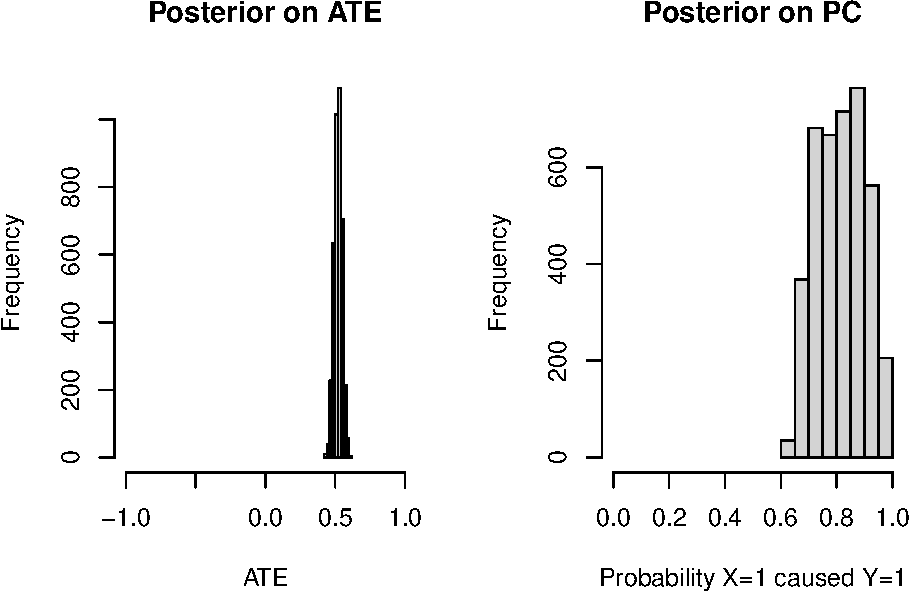
\includegraphics{ii_files/figure-latex/PChist-1} 

}

\caption{ATE is identified, PC is not identified but has informative bounds}\label{fig:PChist}
\end{figure}

The figure illustrates nicely the difference between an identified and non-identified query. While the \(ATE\) converges on the right answer, the probability of causation fails to converge even with a massive amount of data. We see instead a range of values for this query on which our updated model places roughly equal posterior probability.

Importantly, however, we see that we \emph{do} learn about the probability of causation. Despite the lack of convergence, our posterior rules out a wide range of values. While our prior on the query was 0.5, we have correctly updated toward a range of values that includes (and happens to be fairly well centered over) the true value (\(\approx 0.86\)).

A distinctive feature of updating a causal model is that it allows us to learn about non-identified quantities in this manner. We will end up with ``ridges'' in our posterior distributions: ranges or combinations of parameter values that are equally likely given the data. But our posterior weight can nonetheless shift toward the right answer.

At the same time, for non-identified queries, we have to be cautious about the impact of our priors. As \(N\) becomes large, the remaining curvature we see in our posteriors may simply be function of those priors. One way to inspect for this is to simulate a very large dataset and see whether variance shrinks. A second approach is to do sensitivity analyses by updating the model on the same data with different sets of priors to see how this affects the shape of the posterior.

\hypertarget{beyond-binary-data}{%
\subsection{Beyond binary data}\label{beyond-binary-data}}

While the setup used in this book involves only binary nodes, the approach readily generalizes to non-binary data. Moving beyond binary nodes allows for considerably greater flexibility in response functions. For instance, moving from binary to merely 3-level ordinal \(X\) and \(Y\) variables allows us to represent non-linear and even non-monotonic relationships. It also allows us pose more complex queries, such as, ``What is the probability that \(Y\) is linear in \(X\)?'', ``What is the probability that \(Y\) is concave in \(X\)?'', or ``What is the probability that \(Y\) is monotonic in \(X\)?''

To move to non-binary measurement, we need to be able to expand the nodal-type space to accommodate the richer range of possible relations between nodes that can take on more than two possible values. Suppose, for instance, that we want to operate with variables with 4 ordinal categories. In an \(X \rightarrow Y\) model, \(Y\)'s nodal types have to accommodate 4 possible values that \(X\) can take on, and 4 possible values that \(Y\) can take on for any value of \(X\). This yields \(4^4 = 256\) nodal types for \(Y\) and 1024 causal types (compared to just 8 in a binary setup).

The \texttt{CausalQueries} package, set up to work most naturally with binary nodes, can be used to represent non-binary data as well. The trick, as it were, is to express integers in base-2 and then represent the integer as a series of 0's and 1's on multiple nodes. In base-2 counting we would represent four integer values for \(X\) (say, 0, 1, 2, 3) using \(00, 01, 10, 11\). If we use one binary node, \(X_1\) to represent the first digit, and a second node \(X_2\) to represent the second, we have enough information to capture the four values of \(X\). The mapping then is: \(X_1 = 0, X_2 = 0\) represents \(X=0\); \(X_1 = 0, X_2 = 1\) represents \(X=1\); \(X_1 = 1, X_2 = 0\) represents \(X=2\); and \(X_1 = 1, X_2 = 1\) represents \(X=3\). We construct \(Y\) in the same way. We can then represent a simple \(X \rightarrow Y\) relation as a model with two \(X\) nodes each pointing into two \(Y\) nodes: \(Y_1 \leftarrow X_1 \rightarrow Y_2, Y_1 \leftarrow X_2 \rightarrow Y_2\). To allow for the full range of nodal types we need to allow a joint distribution over \(\theta^{X_1}\) and \(\theta^{X_2}\) and over \(\theta^{Y_1}\) and \(\theta^{Y_2}\), which results in 3 degrees of freedom for \(X\) and 255 for \(Y\), as required.

In the illustration below with two 4-level variables, we generate data (\(N=100\)) from a non-monotonic process with the following potential outcomes: \(Y(0)=0, Y(1)=1, Y(2)=3, Y(3) = 2\). We then update and report on posteriors on potential outcomes.

Data from this model looks like this:

\begin{table}[!h]

\caption{\label{tab:unnamed-chunk-13}Data from non binary model (selection of rows)}
\centering
\begin{tabular}[t]{rrrrrr}
\toprule
X1 & X2 & Y1 & Y2 & X & Y\\
\midrule
\cellcolor{gray!6}{0} & \cellcolor{gray!6}{0} & \cellcolor{gray!6}{0} & \cellcolor{gray!6}{0} & \cellcolor{gray!6}{0} & \cellcolor{gray!6}{0}\\
1 & 0 & 1 & 1 & 2 & \vphantom{1} 3\\
\cellcolor{gray!6}{1} & \cellcolor{gray!6}{0} & \cellcolor{gray!6}{1} & \cellcolor{gray!6}{1} & \cellcolor{gray!6}{2} & \cellcolor{gray!6}{3}\\
1 & 1 & 1 & 0 & 3 & 2\\
\bottomrule
\end{tabular}
\end{table}

Updating and querying is done in the usual way:

\begin{table}[H]

\caption{\label{tab:unnamed-chunk-15}Posteriors on potential outcomes for non binary model}
\centering
\begin{tabular}[t]{llrrr}
\toprule
Q & Using & True value & mean & sd\\
\midrule
\cellcolor{gray!6}{Y(0)} & \cellcolor{gray!6}{posteriors} & \cellcolor{gray!6}{0} & \cellcolor{gray!6}{0.37} & \cellcolor{gray!6}{0.08}\\
Y(1) & posteriors & 1 & 0.98 & 0.07\\
\cellcolor{gray!6}{Y(2)} & \cellcolor{gray!6}{posteriors} & \cellcolor{gray!6}{3} & \cellcolor{gray!6}{2.60} & \cellcolor{gray!6}{0.09}\\
Y(3) & posteriors & 2 & 2.02 & 0.07\\
\bottomrule
\end{tabular}
\end{table}

We see that the model performs well. As in the binary setup, the posterior reflects both the data and the priors. And, as usual, we have access to a full posterior distribution over all nodal types and can thus ask arbitrary queries of the updated model.

The greatest challenge posed by the move to non-binary data is computational. If \(Y\) takes on \(m\) possible values and has \(k\) parents, each taking on \(r\) possible values, we then have \(m^{r^k}\) nodal types for \(Y\). Thus, the cost of more granular measurement is complexity -- an explosion of the parameter space -- as the nodal type space expands rapidly with the granularity of measurement and the number of explanatory variables With three 3-level ordinal variables pointing into the same outcome, for instance, we have \(3^{27} = 7.6\) \emph{trillion} nodal types!

We expect that, as measurement becomes more granular, researchers will want to manage the complexity by placing structure onto the possible patterns of causal effects. Structure, imposed through model restrictions, can quite rapidly tame the complexity. For some substantive problems, one form of structure we might be willing to impose is monotonicity. In a \(X \rightarrow Y\) model with 3-level variables, excluding non-monotonic effects brings down the number of nodal types from 27 to 17. Alternatively, we may have a strong reason to rule out effects in one direction: disallowing negative effects, for instance, brings us down to 10 nodal types. If we are willing to assume linearity, the number of nodal types falls further to 5.

\hypertarget{measurement-error}{%
\subsection{Measurement error}\label{measurement-error}}

One potential application of the approach we have described in this chapter to integrating differing forms of data is to addressing the problem of measurement error. The conceptual move to address measurement error in a causal model setup is quite simple: we incorporate the error-generating process into our model.

Consider, for instance, a model in which we build in a process generating measurement error on the dependent variable.

\[X \rightarrow Y  \rightarrow Y_\text{measured} \leftarrow \text{source of measurement error}\]

Here \(X\) has an effect on the true value of our outcome of interest, \(Y\). The true value of \(Y\), in turn, has an effect on the value of \(Y\) that we measure, but so too does a potential problem with our coding process. Thus, the measured value of \(Y\) is a function of both the true value and error.

To motivate the setup, imagine that we are interested in the effect of a rule restricting long-term care staff to working at a single site (\(X\)) on outbreaks of the novel coronavirus in long-term care facilities (\(Y\)), defined as infections among two or more staff or residents. We do not directly observe infections, however; rather, we observe positive results of PCR tests. We also know that testing is neither comprehensive nor uniform. For some units, regular random testing is carried out on staff and residents while in others only symptomatic individuals are tested. It is the latter arrangement that potentially introduces measurement error.

If we approach the problem naively, ignoring measurement error and treating \(Y_\text{measured}\) as though it were identical to \(Y\), a differences in means approach might produce attenuation bias---insofar as we are averaging between the true relationship and 0.

We can do better with a causal model, however. Without any additional data, we can update on both \(\lambda_Y\) and \(\lambda^{Y_\text{measured}}\), and our posterior uncertainty would reflect uncertainty in measurement. We could go further if, for instance, we could reasonably exclude negative effects of \(Y\) on \(Y_\text{measured}\). Then, if we observe (say) a negative correlation between \(X\) and \(Y_\text{measured}\), we can update on the substantive effect of interest -- \(\lambda^Y\) -- in the direction of a larger share of negative effects: it is only \emph{via} negative effects of \(X\) on \(Y\) that a negative correlation between \(X\) and \(Y_\text{measured}\) could emerge. At the same time, we learn about the measure itself as we update on \(\lambda^{Y_\text{measured}}\): the negative observed correlation \(X\) and \(Y_\text{measured}\) is an indicator of the degree to which \(Y_\text{measured}\) is picking up true \(Y\).

We can do better still if we can collect more detailed information on at least some units. One data strategy would be to invest in observing \(Y\), the true outbreak status of each unit, for a subset of units for which we already have data on \(X\) and \(Y_\text{measured}\) --- perhaps by implementing a random-testing protocol at a subset of facilities. Getting better measures of \(Y\) for some cases will allow us to update more directly on \(\lambda^Y\), the true effect of \(X\) on \(Y\), for those cases. But just as importantly, observing true \(Y\) will allow us to update on measurement \emph{quality}, \(\lambda^{Y_\text{measured}}\), and thus help us make better use of the data we have for those cases where we only observe \(Y_\text{measured}\). This strategy, of course, parallels a commonly prescribed use of mixed methods, in which qualitative research takes place in a small set of units to generate more credible measures for large-\(n\) analysis (see, e.g., \citet{seawrightbook}).

In the illustration below, we posit a true average effect of \(X\) on \(Y\) of 0.6. We also posit an average ``effect'' of \(Y\) on measured \(Y\) of just 0.7, allowing for measurement error.

In this setup, with a large amount of data, we would arrive at a differences-in-means estimate of the effect of \(X\) on \emph{measured} \(Y\) of about 0.42. Importantly, this would be the effect of \(X\) on \(Y_{\text{measured}}\) --- not the effect of \(X\) on \(Y\) --- but if we were not thinking about the possibility of measurement error, we would likely conflate the two, arriving at an estimate far from the true value.

We can improve on this ``naive'' estimate in a number of ways using a causal model, as shown in Table \ref{tab:measurmenterror}. First, we can do much better simply by undertaking the estimation within a causal model framework, even if we simply make use of the exact same data. We write down the following simple model \(X \rightarrow Y \rightarrow Y_\text{measured}\), and we build in a monotonicity restriction that disallows negative effects of \(Y\) on \(Y_{\text{measured}}\). As we can see from the first row in Table \ref{tab:measurmenterror}, our mean estimate of the \(ATE\) moves much closer to the true value of 0.6.

Second, we can add data by gathering measures of ``true'' \(Y\) for 20\% of our sample. As we can see from the second row in the table, this investment in additional data does not change our posterior mean much but yields a dramatic increase in precision. In fact, as we can see by comparison to the third row, partial data on ``true'' \(Y\) yields an estimate that is almost the same and almost as precise as the one we would arrive it with data on ``true'' \(Y\) for \emph{all} cases.

\begin{table}

\caption{\label{tab:measurmenterror}Inferences on effects on true Y given measurement error (true ATE = .6)}
\centering
\begin{tabular}[t]{llrr}
\toprule
Data & Using & mean & sd\\
\midrule
\cellcolor{gray!6}{Data on Y measured only} & \cellcolor{gray!6}{posteriors} & \cellcolor{gray!6}{0.64} & \cellcolor{gray!6}{0.09}\\
Data on true Y for 20\% of units & posteriors & 0.63 & 0.03\\
\cellcolor{gray!6}{Data on true Y} & \cellcolor{gray!6}{posteriors} & \cellcolor{gray!6}{0.61} & \cellcolor{gray!6}{0.02}\\
\bottomrule
\end{tabular}
\end{table}

An alternative strategy might involve gathering multiple measures of \(Y\), each with their own independent source of error. Consider the model, \(X \rightarrow Y \rightarrow Y_\text{measured[1]}; Y \rightarrow Y_\text{measured[2]}\). Assume again a true \(ATE\) of \(X\) on \(Y\) of 0.6, that \(Y\) has an average effect of 0.7 on both \(Y_\text{measured[1]}\) and \(Y_\text{measured[2]}\), and no negative effects of true \(Y\) on the measures.\footnote{Importantly, this model assumes nodal types for \(Y_\text{measured[1]}\) and \(Y_\text{measured[2]}\) are independent of one another (no unobserved confounding), implying independent sources of measurement error in this setup.} In this setup, updating on the true \(Y\) can be thought of as a Bayesian version of ``triangulation'', or factor analysis. The results in Table \ref{tab:measurementerror2} are based the same data as in the previous example but now augmented with the second noisy measure for \(Y\).

\begin{table}

\caption{\label{tab:measurementerror2}Inferences on effects on true Y given two noisy measures  (true ATE = .6)}
\centering
\begin{tabular}[t]{llrr}
\toprule
Data & Using & mean & sd\\
\midrule
\cellcolor{gray!6}{Two noisy measures} & \cellcolor{gray!6}{posteriors} & \cellcolor{gray!6}{0.61} & \cellcolor{gray!6}{0.02}\\
\bottomrule
\end{tabular}
\end{table}

As we can see, two noisy measures perform about as well as access to full data on the true \(Y\) (as in Table \ref{tab:measurmenterror}).

The main point here is that measurement error matters for inference and can be taken directly into account within a causal model framework. Confusing measured variables for variables of interest will obviously lead to false conclusions. But if measurement concerns loom large, we can respond by making them part of our model and learning about them. We have illustrated this point for simple setups, but more complex structures could be just as well envisioned, such as those where error is related to \(X\) or, more perniciously, to the effects of \(X\) on \(Y\).

\hypertarget{spillovers}{%
\subsection{Spillovers}\label{spillovers}}

A common threat to causal inference is the possibility of spillovers: a given unit's outcome being affected by the treatment status of another (e.g., possibly neighboring) unit. We can readily set up a causal model to allow for estimation of various quantities related to spillovers.

Consider, for instance, the causal model represented in Figure \ref{fig:spillover}. We consider here groupings of pairs of unit across which spillovers might occur. We might imagine, for instance, a geographically proximate villages separated from other groups such that spillovers might occur between neighboring villages, but can be ruled out across more distal villages. Here \(X_i\) and \(Y_i\) represent village \(i\)'s treatment status and outcome, respectively. The pattern of directed edges indicates that each village's outcome might be affected both by its own and by its neighbors' treatment status.

We now simulate data that allow for spillovers. Specifically, while independently assigning \(X_1\) and \(X_2\) to treatment \(50 \%\) of the time, we (a) set \(Y_1\) equal to \(X_1\), meaning that Unit 1 is affected only by its own treatment status and (b) set \(Y_2\) equal to \(X_1 \times X_2\), meaning that Unit 2 is equally affected by its own treatment status and that of its neighbor, such that \(Y_2 = 1\) only if both Unit 2 and its neighbor are assigned to treatment.

We simulate 100 observations from this data-generating process and then update a model (with flat priors over all nodal types).

\begin{figure}

{\centering 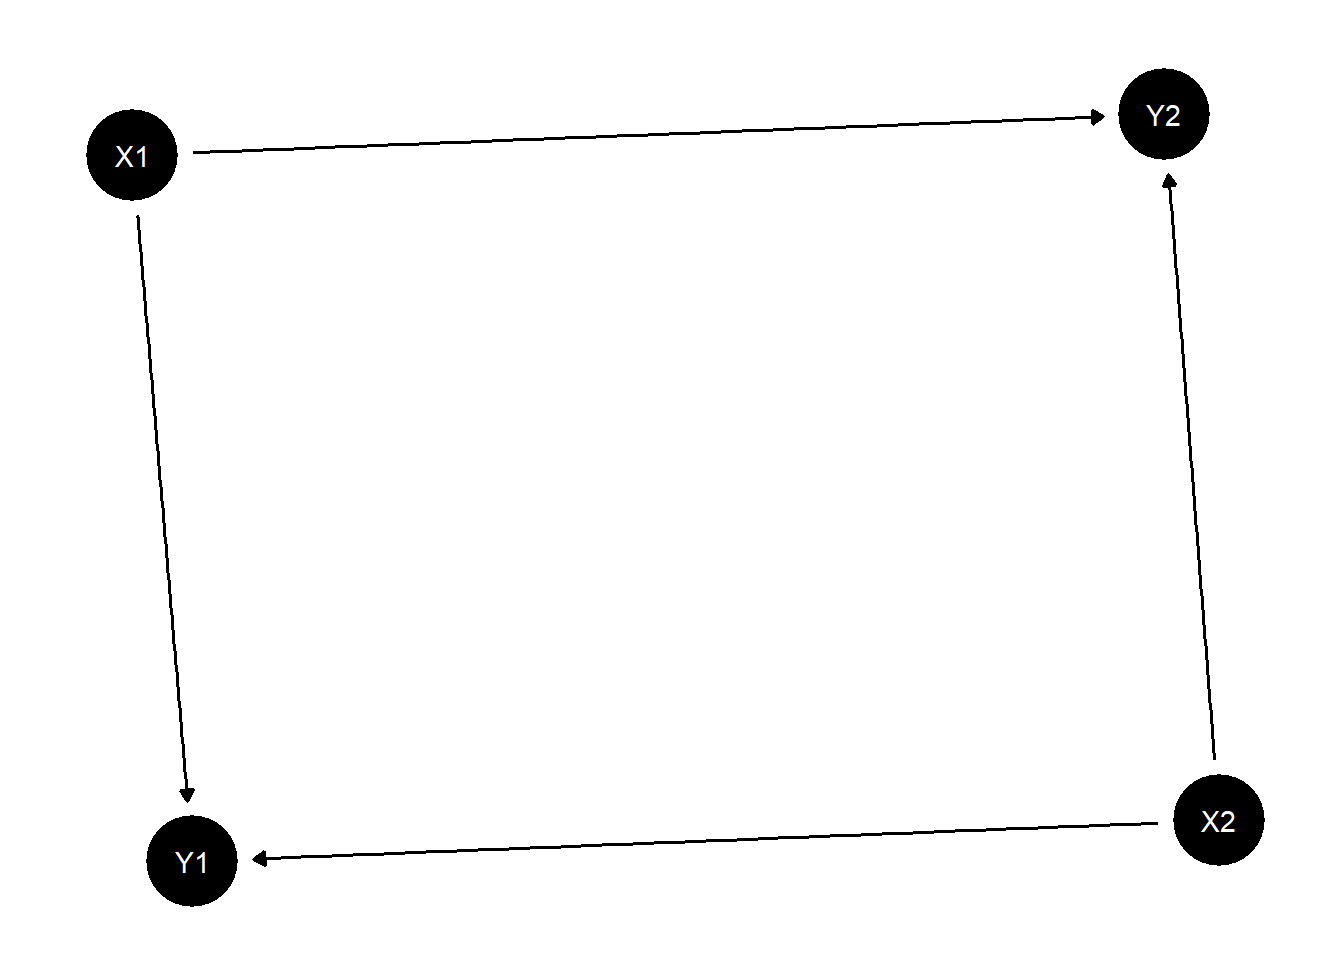
\includegraphics[width=0.5\linewidth]{ii_files/figure-latex/spillover-1} 

}

\caption{Model with spillovers: the treatment status of two units each affect the outcomes for both.}\label{fig:spillover}
\end{figure}

Now we can extract a number of spillover-relevant causal quantities from the updated model. First we ask: what is the average effect of exposing a unit \emph{directly} to treatment (``only\_self\_treated'') when the neighboring unit is untreated? Under the data-generating process that we have posited, we know that this effect will be \(1\) for Unit 1 (which always has a positive treatment effect) and \(0\) for Unit 2 (which sees a positive effect of \(X_2\) only when \(X_1 = 1\)), yielding an average across the two units of \(0.5\). We see that we update, given our 100 observations, from a prior of 0 to a posterior mean of 0.371, approaching the right answer.

A second question we can ask is about the spillover by itself: what is the average treatment effect for a unit of its neighbor being assigned to treatment when the unit itself is not assigned to treatment (``only\_other\_treated'')? We know that the correct answer is \(0\) since Unit 1 responds only to its own treatment status, and Unit 2 requires that both units be assigned to treatment to see an effect. Our posterior estimate of this effect is right on target, at 0.

We can then ask about the average effect of \emph{any} one unit being treated, as compared to no units being treated (``one\_treated''). This is a more complex quantity. To estimate it, we have to consider what happens to the outcome in Unit 1 when only \(X_1\) shifts from control to treatment, with \(X_2\) at control (true effect is \(1\)); what happens to Unit 1 when only \(X_2\) shifts from control to treatment, with \(X_1\) at control (true effect is \(0\)); and the same two effects for Unit 2 (both true effects are \(0\)). We then average across both the treatment conditions and units. We arrive at a posterior mean of \(0.186\), not far from the true value of \(0.25\).

Finally, we can ask about the average effect of both treatments going from control to treatment (``both\_treated''). The true value of this effect is \(1\) for both units, and the posterior has shifted quite far in the direction of this value.

Obviously, more complex setups are possible. We can also model the process in a way that allows for more learning (pooling) across units. In the present model, learning about effects for Unit 1 in a pair tells us nothing about effects for Unit 2 in a pair because they are set up to have completely independent nodal types. We could instead treat all units as drawn from the same population. We could represent this, for instance, in a graph with just one \(Y\) and two treatment nodes pointing into it, one for the unit's own treatment status and one for its neighbor's treatment status.

\begin{table}

\caption{\label{tab:unnamed-chunk-19}Spillover queries}
\centering
\begin{tabular}[t]{llrr}
\toprule
Query & Using & mean & sd\\
\midrule
\cellcolor{gray!6}{only\_self\_treated} & \cellcolor{gray!6}{posteriors} & \cellcolor{gray!6}{0.37} & \cellcolor{gray!6}{0.05}\\
only\_other\_treated & posteriors & 0.00 & 0.04\\
\cellcolor{gray!6}{one\_treated} & \cellcolor{gray!6}{posteriors} & \cellcolor{gray!6}{0.19} & \cellcolor{gray!6}{0.04}\\
both\_treated & posteriors & 0.75 & 0.05\\
\bottomrule
\end{tabular}
\end{table}

\hypertarget{clustering}{%
\subsection{Clustering}\label{clustering}}

We can also represent some forms of clustering, understood as the presence of an exogenous but unobserved factor that influences outcomes for some subgroup of units.

Let us imagine we are looking at the effects of an anti corruption campaign. In some settings we expect this campaign to be effective; in other settings the campaign backfires and has adverse effects. Units vary in whether there are positive or negative effects, but units within the same \emph{cluster} respond similarly. For instance, units in the same village or region. We can represent this situation via the following structural model:

\begin{center}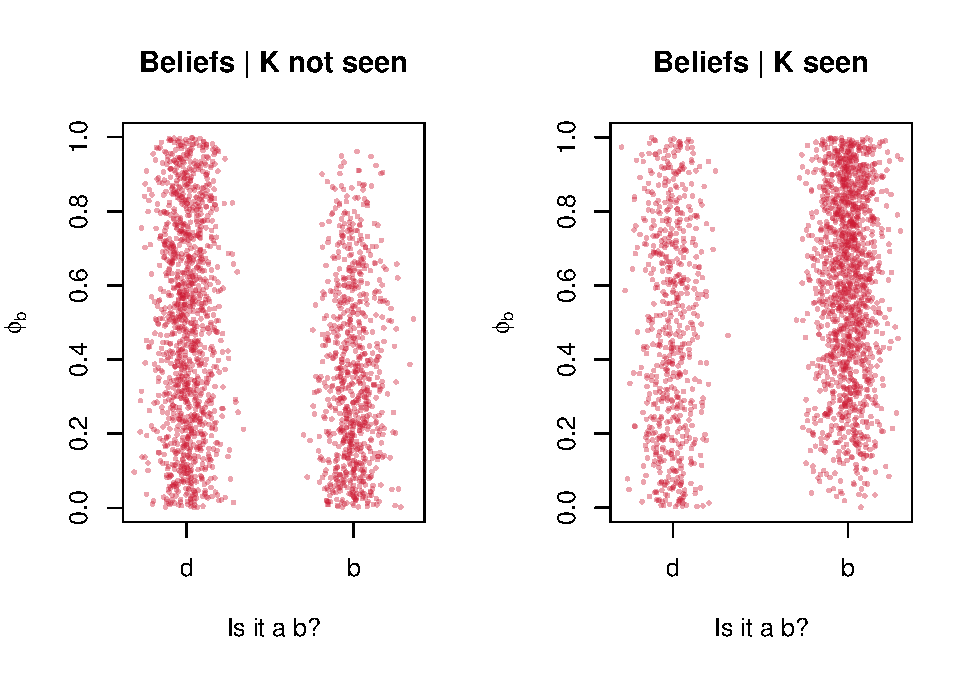
\includegraphics{ii_files/figure-latex/unnamed-chunk-20-1} \end{center}

The graph represents the treatment conditions and the behavior of two officials, both of whom are affected by the same cluster level variable (\(W\)) but who might be exposed to different treatments. By representing this cluster-level factor, \(W\), on the graph, we allow for \emph{learning} across types of units: seeing effects (or non-effects) for one kind of unit allows us to update on \(W\)'s value, which in turn provides information about effects for the other type of unit.

One question we can ask with this setup is: would we learn more from concentrating our observations within a smaller number of clusters or spreading them out across clusters?

In Table \ref{tab:cluster}, we show results from updating on data on four units, with one unit in each of the four \(X/Y\) cells. The difference however is that in one case we imagine the four cases come from four different clusters, and so we learn about the distribution of \(W\) from four clusters. In the other case we imagine the data is drawn from just two clusters (one cluster has the two on diagonal cases, the other has the two off diagonal cases). In this case we learn about \(W\) from only two clusters. The result is greater confidence in the distribution of \(W\), and so greater confidence in our beliefs about causal effects, in the case in which we have data from four clusters.

\begin{table}

\caption{\label{tab:cluster}Data from many pairs is more informative than the same data from fewer pairs.}
\centering
\begin{tabular}[t]{lrr}
\toprule
Data & mean & sd\\
\midrule
\cellcolor{gray!6}{2 obs from each of 2 clusters} & \cellcolor{gray!6}{0} & \cellcolor{gray!6}{0.455}\\
1 obs from each of 4 clusters & 0 & 0.370\\
\bottomrule
\end{tabular}
\end{table}

\hypertarget{mixingapp}{%
\chapter{Integrated Inferences Application}\label{mixingapp}}

\begin{headerbox}
We extend the analysis of Chapter \ref{ptapp} using a model that lets us update about causal processes from data on inequality and democratization from many cases and data on causal processes---mobilization and pressures---from a subset of cases. We then use the updated model to draw both population-level and case-level inferences.

\end{headerbox}

\hypertarget{a-trained-model}{%
\section{A trained model}\label{a-trained-model}}

In Chapter \ref{ptapp} we took the model as given and sought to draw inferences individual cases given data on those cases. In this chapter the model becomes an object that we both learn from and learn about. In essence, we use the data on many cases to update our beliefs about the general model and then use this ``trained'' model to make inferences about cases.

Instead of positing a belief over the nodal types for a given case, \(\theta\), we now need to posit a belief over the \emph{distribution} of nodal types---that is, over \(\lambda\). Whereas in the simple process-tracing model we \emph{specified} the shares of nodal types for \(M\) (for instance), we now specify a prior \emph{distribution} over the nodal type shares. , We do the same, of course, for all nodes. Because we set a prior distribution over nodal types (rather than fixed proportions), we can now update on these population-level distributions as the model confronts data.

The same applies to beliefs about confounding. Recall that we allow for unobserved confounding by allowing \(\lambda\) to include beliefs about the \emph{joint} distributions of nodal types, and we set priors on these joint distributions as well. In the application below, we focus on potential confounding in the relationship between inequality and mobilization: the possibility that inequality may be more or less likely in places where inequality would induce mobilization. Here we do not express informed prior beliefs about the direction or magnitude of such confounding; we set up the parameter matrix to allow for the possibility of confounding and set a flat prior over its direction and magnitude. We can, in turn, learn about confounding from the data.

We begin with the same basic model as we used in Chapter \ref{ptapp}, with inequality (\(I\)) potentially affecting democratization (\(D\)) both through a direct pathway and through an indirect pathway mediated by mobilization (\(M\)). International pressure (\(P\)) is also a ``parent'' of democratization.

Further, we impose the same set of qualitative restrictions, ruling out a negative effect of inequality on mobilization, a direct positive effect of inequality on democratization, a negative effect of mobilization on democracy, and a negative effect of pressure on democratization. Note that this setup allows for inequality to have a positive (through mobilization) effect on democratization, a negative (direct) effect on democratization, or no effect at all.

Finally, we allow for confounding. The theoretical intuition we want to instantiate in the model is that the level of inequality could be endogenous to inequality's effect on mobilization. In particular, in places where mobilization would pose a mobilizational threat, governments may work harder to reduce inequality. To allow for this possibility, we need to create distinct elements of \(\lambda\) representing the conditional distribution of \(I\)'s nodal types given \(M\)'s: one parameter for \(\theta^I\)'s distribution when \(M\)'s nodal type is \(\theta^M_{01}\), and another parameter for \(\theta^I\)'s distribution when \(M\)'s nodal type is something else.

This model, with confounding, is represented graphically as in Figure \ref{fig:pimdgraph}. The possibility of confounding is represented with the bidirected edge, connecting \(I\) and \(M\).

\begin{figure}

{\centering 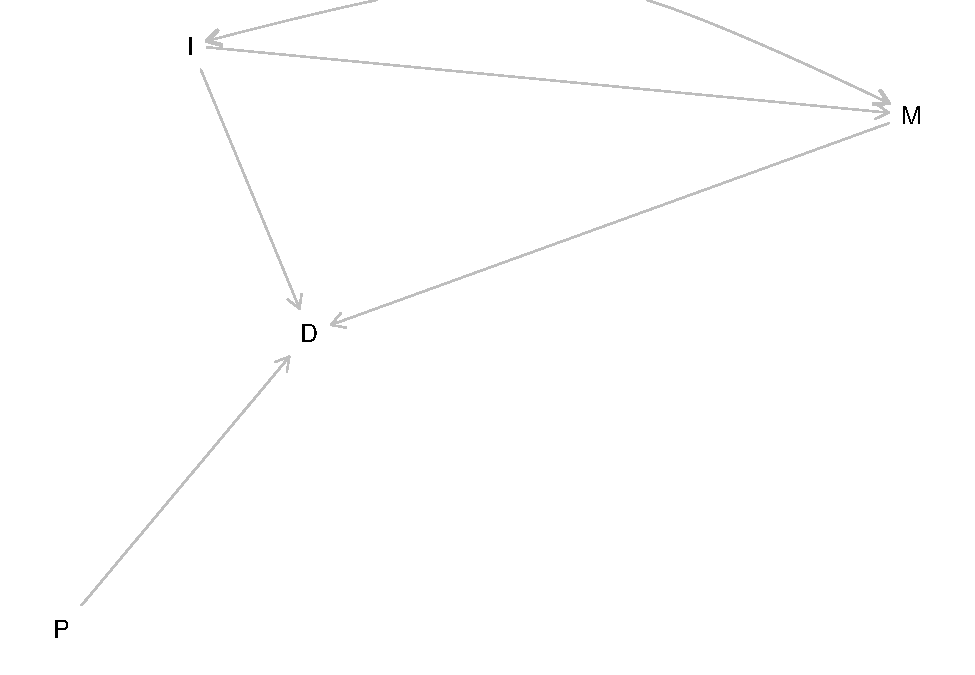
\includegraphics{ii_files/figure-latex/pimdgraph-1} 

}

\caption{Democracy and Inequality Model}\label{fig:pimdgraph}
\end{figure}

\hypertarget{data}{%
\section{Data}\label{data}}

As in Chapter \ref{ptapp}, we will confront the model with data drawn from our coding of the case narratives in the Supplementary Material for \citet{haggard2012inequality}. However, rather than implementing the analysis case-by-case, we now derive leverage from the joint distribution of the data available across all cases.

Table \ref{tab:data82} gives a snapshot of the data.

\begin{table}

\caption{\label{tab:data82}Data (snapshot) derived from Haggard and Kaufman (2012)}
\centering
\begin{tabular}[t]{lrrrr}
\toprule
Case & P & I & M & D\\
\midrule
\cellcolor{gray!6}{Afghanistan} & \cellcolor{gray!6}{} & \cellcolor{gray!6}{1} & \cellcolor{gray!6}{} & \cellcolor{gray!6}{0}\\
Albania & 0 & 0 & 1 & 1\\
\cellcolor{gray!6}{Algeria} & \cellcolor{gray!6}{} & \cellcolor{gray!6}{0} & \cellcolor{gray!6}{} & \cellcolor{gray!6}{0}\\
Angola &  & 1 &  & 0\\
\cellcolor{gray!6}{Argentina} & \cellcolor{gray!6}{0} & \cellcolor{gray!6}{0} & \cellcolor{gray!6}{1} & \cellcolor{gray!6}{1}\\
\addlinespace
Bangladesh & 0 & 0 & 0 & 1\\
\bottomrule
\end{tabular}
\end{table}

Note that this is not a rectangular dataset in that Haggard and Kaufman's collection of clues was conditional on the outcome, \(D=1\): they gathered qualitative data on the presence of international pressure and the presence of mass-mobilization \emph{only} for those cases that democratized. This is not an uncommon case-selection principle. The analyst often reasons that more can be learned about how an outcome arises by focusing in on cases where the outcome of interest has in fact occurred. (We assess this case-selection intuition, in the context of model-based inferences, in Chapter \ref{caseselection}.)

The raw correlations between variables is shown in Table \ref{tab:pimdcorr}. Some correlations are missing because, as mentioned, data on some variables were only gathered conditional on the values of others. For those quantities where we do see correlations, they are not especially strong. There is, in particular, a weak overall relationship between inequality and democratization --- though, of course, this is consistent with inequality having heterogeneous effects across the sample. The strongest correlation in the data is between \(P\) and \(M\), which are assumed to be uncorrelated in the model, though this correlation is also quite weak.

\begin{table}

\caption{\label{tab:pimdcorr}Pairwise correlated in the democracy-inequality (PIMD) data. P = Pressure, I = Inequality, M = Mobilization, D = Democratization}
\centering
\begin{tabular}[t]{lrrrr}
\toprule
  & P & I & M & D\\
\midrule
\cellcolor{gray!6}{P} & \cellcolor{gray!6}{1.000} & \cellcolor{gray!6}{0.157} & \cellcolor{gray!6}{-0.177} & \cellcolor{gray!6}{}\\
I & 0.157 & 1.000 & 0.114 & -0.154\\
\cellcolor{gray!6}{M} & \cellcolor{gray!6}{-0.177} & \cellcolor{gray!6}{0.114} & \cellcolor{gray!6}{1.000} & \cellcolor{gray!6}{}\\
D &  & -0.154 &  & 1.000\\
\bottomrule
\end{tabular}
\end{table}

\hypertarget{inference-1}{%
\section{Inference}\label{inference-1}}

With data and model in hand, we can now update our model to get posteriors on the distribution \(\lambda\) from which we can generate beliefs over all causal relations.

What do we find?

\hypertarget{did-inequality-cause-democratization}{%
\subsection{\texorpdfstring{Did inequality \emph{cause} democratization?}{Did inequality cause democratization?}}\label{did-inequality-cause-democratization}}

We have used the data to update on \(\lambda\): our beliefs about the distributions of nodal types, including about their joint distributions (i.e., confounding). We first use this to make claims about types, similar to what we did in Chapter 8 but now with a model that has been trained on data.

In Table \ref{tab:HK10cases1} we first ask what we would now infer about cases given democratization and low inequality and different observations on mobilization and international pressure. This table is the analogue of Table \ref{tab:HK8cases1} in Chapter \ref{ptapp}.

\begin{table}

\caption{\label{tab:HK10cases1}Four cases with low inequality and  democratization. Question of interest: Was low inequality a cause of democracy? Table shows posterior beliefs for different data for four cases given information on $M$ or $P$. Data from Haggard and Kaufman (2012). Analyses here use a model with assumptions on monotonic effects but magnitudes of effects updated from data.}
\centering
\resizebox{\linewidth}{!}{
\begin{tabular}[t]{lllllll}
\toprule
Case & M: Mobilization? & P: Pressure? & No clues & M only & P only & M and P\\
\midrule
\cellcolor{gray!6}{Mexico (2000)} & \cellcolor{gray!6}{0} & \cellcolor{gray!6}{0} & \cellcolor{gray!6}{0.404} & \cellcolor{gray!6}{0.412} & \cellcolor{gray!6}{0.476} & \cellcolor{gray!6}{0.476}\\
Taiwan (1996) & 0 & 1 & 0.404 & 0.412 & 0.273 & 0.321\\
\cellcolor{gray!6}{Albania (1991)} & \cellcolor{gray!6}{1} & \cellcolor{gray!6}{0} & \cellcolor{gray!6}{0.404} & \cellcolor{gray!6}{0.397} & \cellcolor{gray!6}{0.476} & \cellcolor{gray!6}{0.476}\\
Nicaragua (1984) & 1 & 1 & 0.404 & 0.397 & 0.273 & 0.215\\
\bottomrule
\end{tabular}}
\end{table}

In Table \ref{tab:HK10cases1} we ask what we would now infer about cases given democratization and \emph{high} inequality and different observations on mobilization and international pressure. This table is the analogue of Table \ref{tab:HK8cases2} in Chapter \ref{ptapp}.

\begin{table}

\caption{\label{tab:HK10cases2}Four cases with high inequality and  democratization. Question of interest: Was high inequality a cause of democratization? Table shows posterior beliefs for different data for 4 cases given information on $M$ or $P$. Data from Haggard and Kaufman (2012).  Analyses here use a model with assumptions on monotonic effects but magnitudes of effects updated from data.r}
\centering
\resizebox{\linewidth}{!}{
\begin{tabular}[t]{lllllll}
\toprule
Case & M: Mobilization? & P: Pressure? & No clues & M only & P only & M and P\\
\midrule
\cellcolor{gray!6}{Mongolia (1990)} & \cellcolor{gray!6}{0} & \cellcolor{gray!6}{0} & \cellcolor{gray!6}{0.118} & \cellcolor{gray!6}{0} & \cellcolor{gray!6}{0.157} & \cellcolor{gray!6}{0}\\
Paraguay (1989) & 0 & 1 & 0.118 & 0 & 0.064 & 0\\
\cellcolor{gray!6}{Sierra Leone (1996)} & \cellcolor{gray!6}{1} & \cellcolor{gray!6}{0} & \cellcolor{gray!6}{0.118} & \cellcolor{gray!6}{0.161} & \cellcolor{gray!6}{0.157} & \cellcolor{gray!6}{0.205}\\
Malawi (1994) & 1 & 1 & 0.118 & 0.161 & 0.064 & 0.093\\
\bottomrule
\end{tabular}}
\end{table}

\hypertarget{did-inequality-prevent-democracy}{%
\subsection{\texorpdfstring{Did inequality \emph{prevent} democracy?}{Did inequality prevent democracy?}}\label{did-inequality-prevent-democracy}}

As before we can also ask questions about causes that have not democratized -- even though we have no additional data about these cases in particular.

We see answers in Tables \ref{tab:Tapp101} and \ref{tab:Tapp102}. Among cases with low inequality, we infer that low inequality was a cause of non democratization especially if we \emph{do} see external pressure but we do \emph{not} see mobilization. If we do see mobilization we do not attribute the failure to democratize to the low inequality---greater inequality would not have made a difference via mobilization since populations were mobilized already. Among cases with high inequality and no democratization we think that the inequality was preventing the democratization especially in cases where we see mobilization and pressure---factors that would otherwise have favored democratization.

Overall the patterns are very similar here to what we saw in Chapter \ref{ptapp}, though slightly stronger in the case of low inequality and slightly weaker in the case of higher inequality.

\begin{table}

\caption{\label{tab:Tapp101}No inequality and No democratization: Was no inequality a cause of no democratization? Analyses here use priors assuming only monotonic effects.}
\centering
\begin{tabular}[t]{lrrr}
\toprule
  & P & M & posterior\\
\midrule
\cellcolor{gray!6}{I0P0M0D0} & \cellcolor{gray!6}{0} & \cellcolor{gray!6}{0} & \cellcolor{gray!6}{0.127}\\
I0P1M0D0 & 1 & 0 & 0.269\\
\cellcolor{gray!6}{I0P0M1D0} & \cellcolor{gray!6}{0} & \cellcolor{gray!6}{1} & \cellcolor{gray!6}{0.000}\\
I0P1M1D0 & 1 & 1 & 0.000\\
\cellcolor{gray!6}{I0M0D0} & \cellcolor{gray!6}{} & \cellcolor{gray!6}{0} & \cellcolor{gray!6}{0.145}\\
\addlinespace
I0M1D0 &  & 1 & 0.000\\
\cellcolor{gray!6}{I0P0D0} & \cellcolor{gray!6}{0} & \cellcolor{gray!6}{} & \cellcolor{gray!6}{0.101}\\
I0P1D0 & 1 &  & 0.244\\
\cellcolor{gray!6}{I0D0} & \cellcolor{gray!6}{} & \cellcolor{gray!6}{} & \cellcolor{gray!6}{0.117}\\
\bottomrule
\end{tabular}
\end{table}

\begin{table}

\caption{\label{tab:Tapp102}Inequality and No democratization: Was inequality a cause of no democratization? Analyses here use priors assuming only monotonic effects.}
\centering
\begin{tabular}[t]{lrrr}
\toprule
  & P & M & posterior\\
\midrule
\cellcolor{gray!6}{I1P0M0D0} & \cellcolor{gray!6}{0} & \cellcolor{gray!6}{0} & \cellcolor{gray!6}{0.246}\\
I1P1M0D0 & 1 & 0 & 0.565\\
\cellcolor{gray!6}{I1P0M1D0} & \cellcolor{gray!6}{0} & \cellcolor{gray!6}{1} & \cellcolor{gray!6}{0.392}\\
I1P1M1D0 & 1 & 1 & 0.659\\
\cellcolor{gray!6}{I1M0D0} & \cellcolor{gray!6}{} & \cellcolor{gray!6}{0} & \cellcolor{gray!6}{0.308}\\
\addlinespace
I1M1D0 &  & 1 & 0.424\\
\cellcolor{gray!6}{I1P0D0} & \cellcolor{gray!6}{0} & \cellcolor{gray!6}{} & \cellcolor{gray!6}{0.311}\\
I1P1D0 & 1 &  & 0.595\\
\cellcolor{gray!6}{I1D0} & \cellcolor{gray!6}{} & \cellcolor{gray!6}{} & \cellcolor{gray!6}{0.357}\\
\bottomrule
\end{tabular}
\end{table}

\hypertarget{from-cases-to-population}{%
\section{From cases to population}\label{from-cases-to-population}}

One set of questions we can ask of the updated model is about the probability that high inequality causes democratization. We can pose this question at different levels of conditioning. For instance, we can ask:

\begin{enumerate}
\def\labelenumi{\arabic{enumi}.}
\item
  \textbf{For all cases}. For what proportion of cases in the population does inequality have a positive effect on democratization?
\item
  \textbf{For all cases displaying a given causal state and outcome}. Looking specifically at those cases that in fact had high inequality and democratized, for what proportion was the high inequality a cause of democratization?
\item
  \textbf{For cases displaying a given causal state and outcome, and with additional clues present or absent.} What if we have also collected clues on mediating or moderating nodes? For instance, for what proportion of high-inequality, democratizing cases \emph{with} mobilization did inequality cause the outcome? For what proportion \emph{without} mobilization? Likewise for the presence or absence of international pressure? Importantly, comparing a given estimate with and without a given clue amounts to an assessment of the clue's probative value.
\end{enumerate}

We ask \texttt{CausalQueries} now to query \(\lambda\)'s posterior distribution to generate posterior distributions for each of these quantities. We can define our queries quite simply in terms of the causal types that correspond to the effect of interest and then take the conditional probability of these. We present the code and results of these operations below and in Figure \ref{fig:mixedhist}.

\begin{table}

\caption{\label{tab:unnamed-chunk-22}Probability that inequality increases chances of democratization given:}
\centering
\begin{tabular}[t]{lr}
\toprule
Given & mean\\
\midrule
\cellcolor{gray!6}{-} & \cellcolor{gray!6}{0.04}\\
D==1 \& I==1 & 0.12\\
\cellcolor{gray!6}{D==1 \& I==1 \& M==1} & \cellcolor{gray!6}{0.16}\\
D==1 \& I==1 \& M==0 & 0.00\\
\cellcolor{gray!6}{D==1 \& I==1 \& M==1 \& P==1} & \cellcolor{gray!6}{0.09}\\
\addlinespace
D==1 \& I==1 \& M==1 \& P==0 & 0.21\\
\bottomrule
\end{tabular}
\end{table}

In figure \ref{fig:mixedhist}, we graph the priors for each of these queries next to the posteriors.

\begin{figure}

{\centering 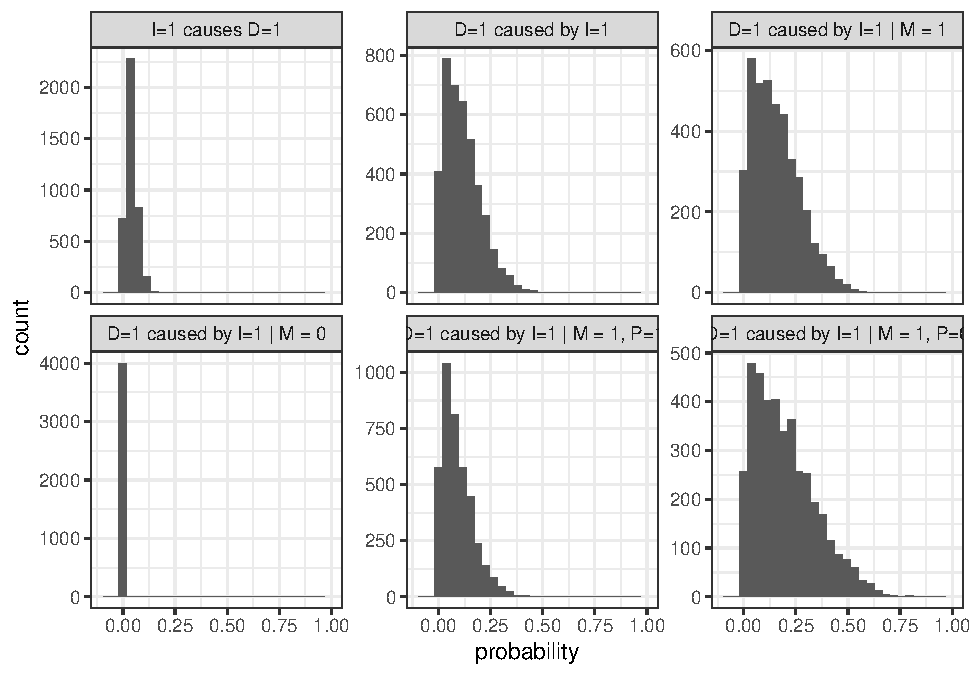
\includegraphics{ii_files/figure-latex/mixedhist-1} 

}

\caption{Posteriors on Causes of Democratization}\label{fig:mixedhist}
\end{figure}

We can see that the share of cases overall in which inequality causes democratization is estimated to be very low, with a good deal of confidence. The proportion is considerably higher for those cases that in fact experienced high inequality and democratization. The proportion of positive causal effects is believed to be even higher for those in which mobilization occurred. Moreover, the proportion of \(I=1, D=1\) cases with a positive effect of inequality on democratization is even higher when an alternative cause---international pressure---is absent, though our uncertainty about this share is also very high.

We also see that the absence of mobilization tells us for certain that democratization was not caused by inequality. Interestingly, however, this result derives purely from the model restrictions, rather than from the data: under the restrictions we imposed, a positive effect of inequality can operate \emph{only} through mobilization.

Turning now to the cases in which democratization did not occur, Figure \ref{fig:mixedhist2} asks for what proportion of cases overall inequality has a negative effect on democratization; for what proportion of \(I=1, D=0\) cases inequality prevented democratization; and this latter query conditional on different clue realizations.

\begin{figure}

{\centering 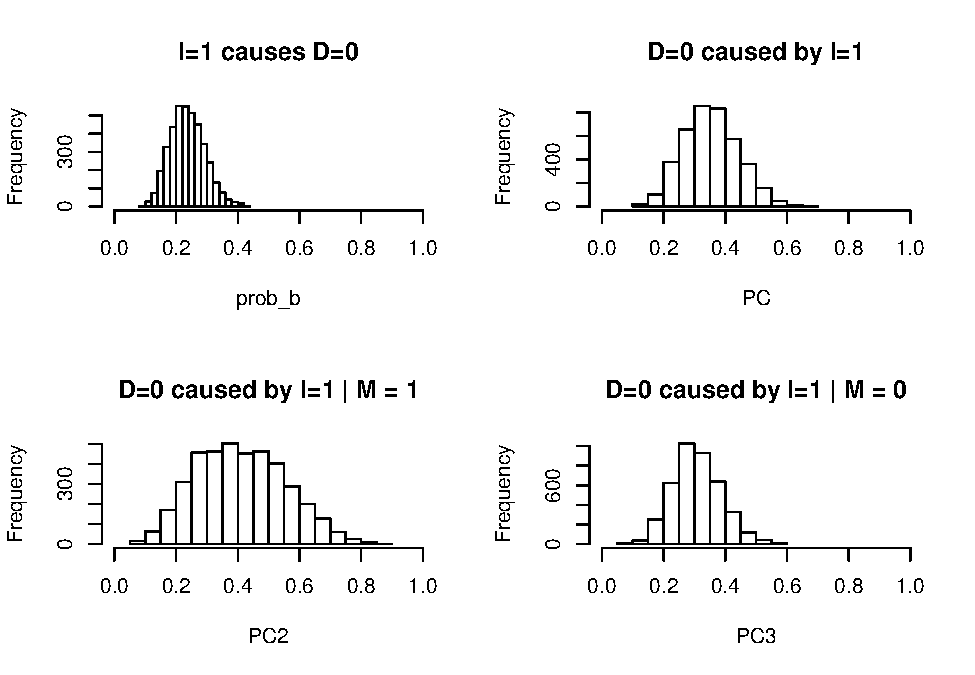
\includegraphics{ii_files/figure-latex/mixedhist2-1} 

}

\caption{Posteriors on Causes of Democratization}\label{fig:mixedhist2}
\end{figure}

We see that inequality appears, overall, more commonly to prevent democratization than to cause it. We are, moreover, most confident that inequality played a preventive role in those cases in which there was mobilization and international pressure---both of which \emph{could} have generated democratization---but still no democratization occurred.

\hypertarget{contribution-to-case-level-inference}{%
\subsection{Contribution to case-level inference}\label{contribution-to-case-level-inference}}

There are two ways of thinking about the learning we derive from the above estimates. On the one hand, we can think of our estimands in population-level terms. The results in Figures \ref{fig:mixedhist} and \ref{fig:mixedhist2} can be understood as our estimates of the \emph{share} of cases in the population, with a given set of characteristics, for which a particular causal effect holds.

Yet these distributions, by the very same token, represent our beliefs about the probability that \(I\) had a positive or negative (depending on the query we are talking about) causal effect in an individual case for which we have seen a given data pattern. Thus, for instance, from Figure \ref{fig:mixedhist} we can see our posterior belief about the proportion of \(I=D=M=1\) cases in the population for which \(I=1\) caused \(D=1\). But this also tells us, for an individual case randomly selected from the population of \(I=D=M=1\) cases, the probability that high inequality caused democratization in the case. To put the point differently, suppose we want to know whether \(I=1\) was a cause of \(D=1\) in a randomly selected case, so we do process tracing and observe \(M=1\): this same estimate answers the case-level query, telling us the probability that \(I=1\) caused \(D=1\) in the case at hand.

The key difference between case-level inference from mixed data and the pure process-tracing setup from Chapter \ref{ptapp} is that now our case-level inferences are informed by \emph{data} from the population, rather than merely by a set of prior beliefs about the population. Consider, for instance, the difference in posteriors on the probability of a negative effect for the query for \(I=1, D=0\) given \(M=0\) (mean of about 0.31) as compared to the query for \(I=1, D=0\) given \(M=1\) (about 0.42). That difference in what we believe depending on \(M\)'s value represents the probative value of the \(M\) clue given the model as \emph{updated} from the data. Of course, we have also made assumptions in building the model, including motonicity restrictions, and we speak to their role below. But the general point is that, in mixed-data inference, we can learn empirically about the probative value of any given node, rather than drawing probative value purely from theory.

\hypertarget{how-much-do-we-get-from-the-model-vs.-the-data}{%
\subsection{How much do we get from the model vs.~the data?}\label{how-much-do-we-get-from-the-model-vs.-the-data}}

We might wonder, at the same time, how much we are in fact learning from the data, as compared to what we built into the model at the outset, including through the monotonicity restrictions that we imposed. To examine this, in Figures \ref{fig:dcaused} and \ref{fig:dprevented}, we plot the mean (and one-standard-deviation error bars) of our prior and our posterior on the same set of queries. We see that there is almost no shift in beliefs for the positive-effect queries, with a somewhat greater shift in means for the negative-effect queries. However, our uncertainty about negative effects shrinks some, though remains quite high.

By comparing the prior and posterior estimates given \(M=1\) and given \(M=0\), we can also assess whether we have learned about \(M\)'s informativeness. We see that, in this example, we do not happen to learn anything from the data about \(M\)'s probative value: the difference in beliefs between each estimate given \(M=1\) and that estimate given \(M=0\) remains about the same in our posteriors as it was in our priors.

\begin{figure}

{\centering 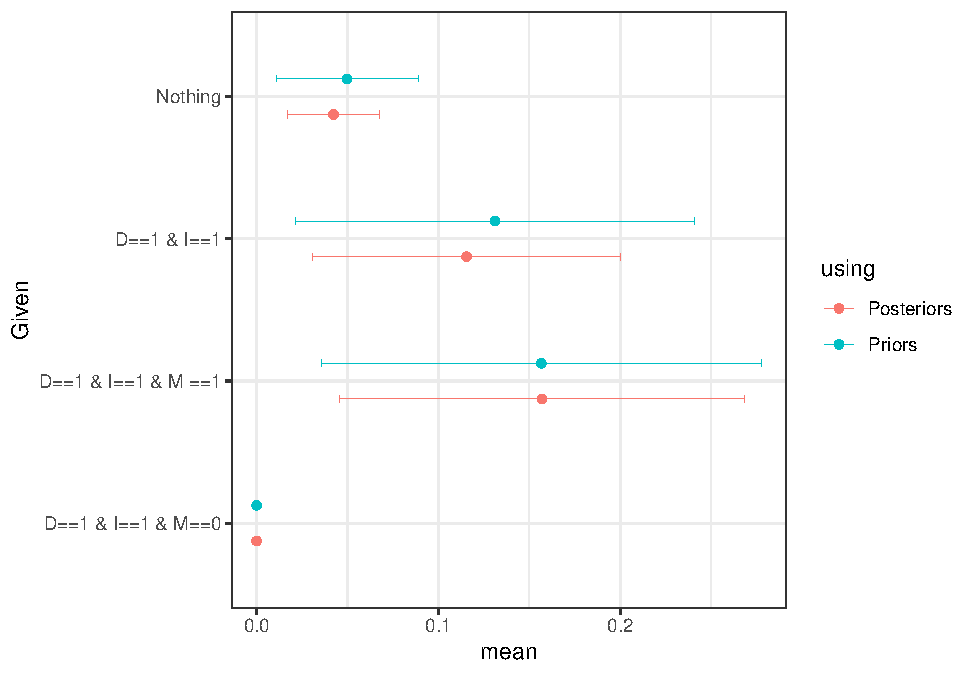
\includegraphics{ii_files/figure-latex/dcaused-1} 

}

\caption{Priors and posteriors on the probability that inequality caused democratization (probability that I has a positive effect on D) given different kinds of observed case-level data. The error bars show plus or minus one standard deviation of the posterior variance. }\label{fig:dcaused}
\end{figure}

\begin{figure}

{\centering 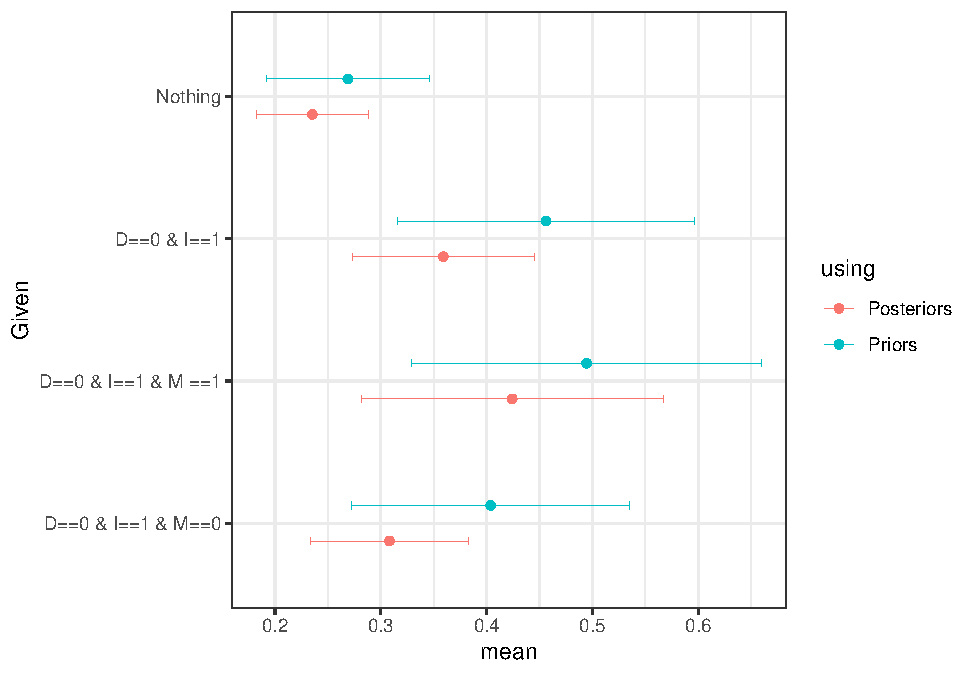
\includegraphics{ii_files/figure-latex/dprevented-1} 

}

\caption{Priors and posteriors on the probability that inequality prevented democratization (probability that I has a negative effect on D) given different kinds of observed case-level data. The error bars show plus or minus one standard deviation of the respective distribution's variance.}\label{fig:dprevented}
\end{figure}

\hypertarget{mm}{%
\chapter{Mixing models}\label{mm}}

\begin{headerbox}
We provide four examples of situations in which, by combining models, researchers learn more than they could from any single model.

\end{headerbox}

In the previous two chapters, we described one form of integration that structural causal models can enable: the systematic combination of (what we typically think of as) qualitative and quantitative evidence for the purposes of drawing population- and case-level causal inferences. One feature of the analyses we have been considering so far is that the integration is essentially ``nested.'' We are, for instance, integrating quantitative evidence for a large set of cases with qualitative evidence for a \emph{subset} of those cases. We are, moreover, drawing inferences from the set of cases we observe to a population \emph{within which} that sample of cases is situated.

In this chapter, we examine how we can use structural causal models to integrate across studies or settings that are, in a sense, more disjointed from one another: across studies that examine different causal relationships altogether; study designs that require different assumptions about exogeneity; and contexts across which the causal quantities of interest may vary.

\begin{enumerate}
\def\labelenumi{\arabic{enumi}.}
\item
  \textbf{Integrating across a model} Often, individual studies in a substantive domain examine distinct segments of a broader web of causal relationships. For instance, while one study might examine the effect of \(X\) on \(Y\), another might examine the effect of \(Z\) on \(Y\), and yet another might examine the effect of \(Z\) on \(K\). We show in this chapter how we can integrate across such studies in ways that yield learning that we could not achieve by taking each study on its own terms.
\item
  \textbf{Integrating between experimental and observational studies} One form of multi-method research that has become increasingly common is the use of both observational and experimental methods to study the same basic causal relationships. While an experiment can offer causal identification in a usually local or highly controlled setting, an observational analysis can often shed light on how the same relationships operate ``in the wild,'' if with greater risk of confounding. Usually, observational and experimental results are presented in parallel, as separate sources of support for a causal claim. We show how, in a causal model setup, we can use experimental and observational data \emph{jointly} to address questions that cannot be answered when the designs are considered separately.
\item
  \textbf{Transporting knowledge across contexts} Researchers are sometimes in a situation in which they can identify causal quantities in a particular setting --- say, from a randomized controlled trial implemented in a specific local context --- but want to know how those inferences travel to other settings. Would the intervention work differently in other countries or regions? As we will explain, with an appropriately specified causal model and the right data from the original context, we can draw inferences about causal relationships in other contexts.
\item
  \textbf{Models in hierarchies.} Sometimes researchers learn about the same types of processes in different settings. By thinking of the processes in each setting as deriving from a family of processes, researchers can learn from observations in one setting about causal processes in another and also learn about the nature of heterogeneity between settings.
\end{enumerate}

Before delving into the details of these strategies, we make one key qualification explicit: each of these approaches requires us to believe that setting-, or study-, specific causal model can be nested within a lower level, ``encompassing,'' model that operates across the multiple settings that we are learning from and want to draw inferences about. Encompassing models, of course, can specifically take heterogeneity across settings into account, for instance by including in the model moderators that condition the effects of interest. But we have to believe that we have indeed captured in the model any ways in which relationships vary across the set of contexts across which we are integrating evidence or transporting inferences.

Put differently, and perhaps more positively, we see social scientists commonly seeking to transport knowledge or combine information informally across studies and settings. Often such efforts are motivated, sometimes implicitly, by an interest in or reliance on general theoretical propositions. The approaches that we describe below force the researcher to be \emph{explicit} about the underlying causal beliefs that warrant that integration while also ensuring that the integration proceeds in a way that is logically consistent with stated beliefs.

\hypertarget{a-jigsaw-puzzle-integrating-across-a-model}{%
\section{A jigsaw puzzle: Integrating across a model}\label{a-jigsaw-puzzle-integrating-across-a-model}}

Generating knowledge about a causal domain often involves cumulating learning across studies that each focus in on some specific part of the domain. For instance, scholars interested in the political economy and democratization might undertake studies focused on the relationship between inequality and mass protests; studies on the role of mass mobilization in generating regime change; pathways other than mass mobilization through which inequality might affect democratization; studies of the role of international sanctions on the likelihood that autocracies will democratize; and studies of the effects of democratization on other things, such as growth or the distribution of resources.

We can think of these studies as each analyzing data on a particular part of a broader, more encompassing causal model. In an informal way, \emph{if} findings ``hold together'' in a reasonably intuitive way, we might be able to piece together an impression of the overall relations among variables in this domain. Yet an informal approach becomes more difficult for complex models or data patterns and, more importantly, will leave opportunities for learning unexaploited.

Consider this simple DAG, in which both \(X\) and \(Z\) are causes of \(Y\), and \(Z\) also causes \(K\). Now imagine three studies, all conducted in contexts in which we believe this model to hold:

\begin{center}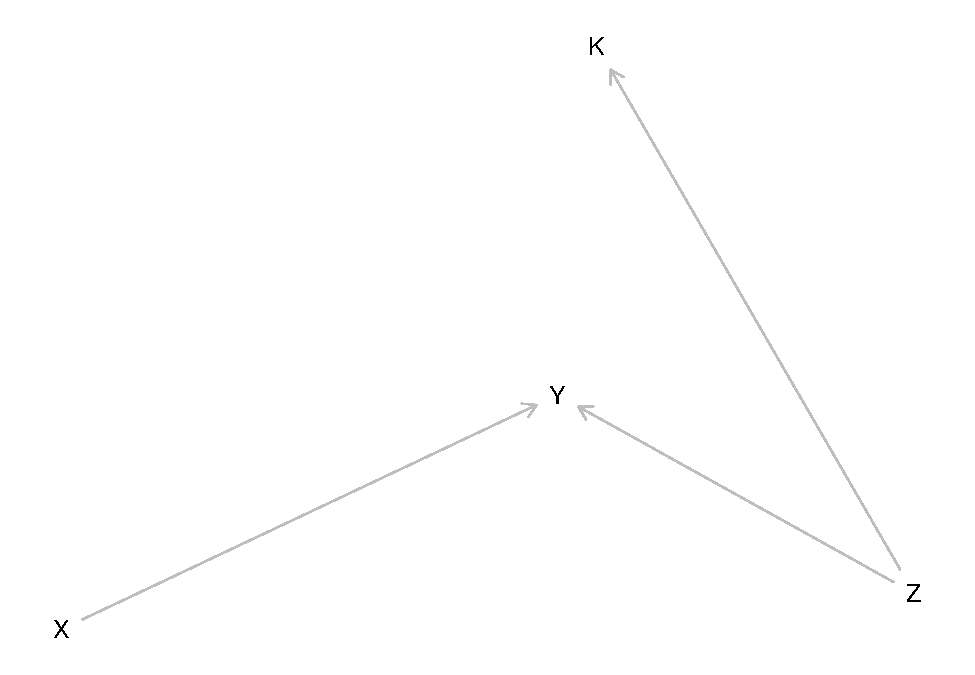
\includegraphics{ii_files/figure-latex/jigsaw-1} \end{center}

\begin{enumerate}
\def\labelenumi{\arabic{enumi}.}
\tightlist
\item
  Study 1 is an RCT in which \(X\) is randomized, with data collected on both \(Y\) and \(K\). \(K\) is collected. \(Z\) is not observed.
\item
  Study 2 is a factorial experiment, in which \(X\) and \(Z\) are independently randomized, allowing an examination of the joint effects of \(X\) and \(Z\) on \(Y\). \(K\) is not observed.
\item
  Study 3 is an experiment randomizing \(Z\), with only \(K\) observed as an outcome. \(X\) and \(Y\) are not observed.
\end{enumerate}

Now, let's say that our primary interest is in the relationship between \(X\) and \(Y\). Obviously, Study 1 will, with a sufficiently large sample, perform just fine in estimaing the average treatment effect of \(X\) on \(Y\). However, what if we are interested in a case-oriented query, such as the probability of causation: the probability, say, \(X=1\) caused \(Y=1\) in a given \(X=1, Y=1\) case?

We know that within-case, process-tracing clues can sometimes provide probative value on case-level estimands like the probability of causation, and we have observed \(K\) in the Study 3 cases. So what if we combine the \(X\), \(Y\), and \(K\) data?

A simple analysis of the graph tells us that \(K\) cannot help us learn about \(Y\)'s potential outcomes since \(K\) and \(Y\) are \(d\)-separated by \(Z\), and we have not observed \(Z\) in Study 3. We see this confirmed in Table \ref{tab:frank1}.

In the first pair of rows, we show the results of analyses in which we have simulated data from the whole model, then updated using the Study 1 observations. We give here the posterior mean on the probability of causation for an \(X=Y=1\) case, conditional on each possible value that \(K\) might take on. As we can see, our beliefs about the estimand remain unaffected by \(K\)'s value, meaning that it contains no information about \(X\)'s effect in the case.

We see that the same thing is true for each of the other studies. In study 2, we have not used \(K\) to update the model, and so have not learned anything form the data about \(K\)'s relationship to the other variables. Thus, we have no foundation on which to ground probative value fo \(K\). In study 3, we understand the \(Z,K\) relationship well, but know nothing quantitatively about how \(Z\) and \(X\) relate to \(Y\). Thus, we have learned nothing from Study 3 about what observing \(K\) might tell us about the effect of \(X\) on \(Y\).

\begin{table}

\caption{\label{tab:frank1}The clue $K$ uninformative in all three studies}
\centering
\begin{tabular}[t]{rlrr}
\toprule
Study & Given & mean & sd\\
\midrule
\cellcolor{gray!6}{1} & \cellcolor{gray!6}{X == 1 \& Y == 1 \& K == 1} & \cellcolor{gray!6}{0.592} & \cellcolor{gray!6}{0.126}\\
 & X == 1 \& Y == 1 \& K == 0 & 0.508 & 0.119\\
\cellcolor{gray!6}{2} & \cellcolor{gray!6}{X == 1 \& Y == 1 \& K == 1} & \cellcolor{gray!6}{0.650} & \cellcolor{gray!6}{0.122}\\
 & X == 1 \& Y == 1 \& K == 0 & 0.651 & 0.124\\
\cellcolor{gray!6}{3} & \cellcolor{gray!6}{X == 1 \& Y == 1 \& K == 1} & \cellcolor{gray!6}{0.500} & \cellcolor{gray!6}{0.158}\\
\addlinespace
 & X == 1 \& Y == 1 \& K == 0 & 0.500 & 0.134\\
\bottomrule
\end{tabular}
\end{table}

We can do much better, however, if we combine the data and update \emph{jointly} across all model paramaters. The results are shown in Table \ref{tab:frank4}. Updating simultaneously across the studies allows us, in a sense, to bridge across inferences. In particular, inferences from Study 2 make \(Z\) informative about \(Y\)'s potential outcomes under different values of \(X\). Meanwhile, inferences from the data in Study 3 allow us to use information on \(K\) to update on values for \(Z\). As we now see in rows 1 and 2, having updated the model in an integrated fashion, \(K\) now \emph{is} informative about the probability of causation, with our posterior mean on this query changing substantially depending on the value of \(K\) that we observe in a case.

Rows 3-4 highlight that the updating works through inferences on \(Z\): we see that if \(Z\) is already known (we show this for \(Z=1\), but it holds for \(Z=0\) as well), then there are no additional gains from knowledge of \(K\).

\begin{table}

\caption{\label{tab:frank4}Clue is informative after combining studies linking $K$ to $Z$ and $Z$ to $Y$}
\centering
\begin{tabular}[t]{lrr}
\toprule
Given & mean & sd\\
\midrule
\cellcolor{gray!6}{X == 1 \& Y == 1 \& K == 1} & \cellcolor{gray!6}{0.80} & \cellcolor{gray!6}{0.09}\\
X == 1 \& Y == 1 \& K == 0 & 0.55 & 0.14\\
\cellcolor{gray!6}{X == 1 \& Y == 1 \& K == 1 \& Z == 1} & \cellcolor{gray!6}{0.82} & \cellcolor{gray!6}{0.09}\\
X == 1 \& Y == 1 \& K == 0 \& Z == 1 & 0.82 & 0.09\\
\bottomrule
\end{tabular}
\end{table}

We devote Chapter \ref{justifying} to a discussion of how we justify a model. However, we note already that in this example we have an instance in which a researcher (examining a case in study 3) might wish to draw inferences using \(K\), but she does not have anything in study 1 that justifies using \(K\) for inference. However with access to studies 2 and 3, and conditional on the overall model, she has a justification for process tracing strategy. The general principle is that weaker commitments to lower level theories ---here the causal structure---can justify more fully inferences from more fully specified higher-level theories.

\hypertarget{combining-observational-and-experimental-data}{%
\section{Combining observational and experimental data}\label{combining-observational-and-experimental-data}}

Experimental studies are often understood as the ``gold standard'' for causal inference. This is, in particular, because of the ability of a randomized trial (given certain assumptions, such as ``no spillovers'') to eliminate sources of confounding. By design, an experiment removes from the situation processes that, in nature, would generate a correlation between selection into treatment and potential outcomes. An experiment thereby allows for an unbiased estimate of the average causal effect of the treatment on the outcome.

At the same time, an interesting weakness of experimental studies is that, by dealing so effectively with selection into treatment, they limit our ability to learn about selection and its implications in the real world. Often, however, we want to know what causal effects would be specifically for units that \emph{would} in fact take up a treatment in a real-world, non-experimental settings. This kind of problem is studied for example by \citet{knox2019design}.

Consider, for instance, a policy that would make schooling subsidies available to parents, with the aim of improving educational outcomes for children. How would we know if the policy was effective? A source of confounding in an observational setting might be that those parents who apply for and take up the subsidy might also be those who are investing more in their children's education in other ways as compared to those parents who do not apply for the subsidy. To eliminate this problem, we might design an experiment in which parents are randomly assigned to receive (or not receive) the subsidy and compare outcomes between children in the treatment and control groups. With a no-spillovers assumption, we can extract the \(ATE\) of the receipt of subsidies.

What this experiment cannot tell us, however, is how much the policy will boost educational outcomes outside the experiment. That is because the causal quantity of interest, for answering that question, is \emph{not} the \(ATE\): it is the average treatment effect for the \emph{treated} (\(ATT\)), given real-world selection effects. That is, the policymaker wants to know what the effect of the subsidy will be for the children of parents who \emph{select into} treatment. One could imagine the real-world \(ATT\) being higher than the \(ATE\) if, for instance, those parents who are informed and interested enough to take up the subsidy also put the subsidy to more effective use. One could also imagine the \(ATT\) being lower than the \(ATE\) is, for instance, there are diminishing marginal returns to educational investments and the self-selecting parents are already investing quite a lot.

Even outside a policy context, we may be interested in the effect of a causal condition \emph{where} that causal condition emerges. To return to our inequality and democracy example, we may want to know what would have happened to autocracies with low inequality \emph{if} they had had high inequality -- the standard average-treatment effect question. But we might also be interested in knowing how much of a difference high inequality makes \emph{in the kinds of cases} where high inequality tends to be occur -- where the effect could be very different.

With such questions, we are in a sort of bind. The experiment cannot tell us \emph{who} would naturally select into treatment and what the effects would be for them. Yet an observational study faces the challenge of ruling out confounding. Ideally, we would like to be able to combine the best features of both: use an experiment to deal with confounding and use observational data to learn about those whom nature assigns to treatment.

We can achieve this form of integration with a causal model. We do so by creating a model in which random assignment is nested within a broader set of assignment processes. We plot the model in Figure \ref{fig:appcombexpob}

At the substantive core of this model is the \(X \rightarrow Y\) relationship. However, we give \(X\) a parent that is fully exogenous, \(Z\), to capture a random-assignment process. We give \(X\) a second parent, \(O\), that is confounded with \(Y\): \(O\) here represents the observational scenario. Finally, we include a ``switch'' variable, \(R\), that determines whether \(X\) is randomly assigned or not. So when \(R=1\), \(X\) is determined solely by \(Z\), with \(X=Z\). When \(R=0\), we are in an observational setting, and \(X\) is determined solely by the confounded \(O\), with \(X=O\).

A few notes on the parameter space. Parameters allow for complete confounding between \(O\) and \(Y\), but \(Z\) and \(Y\) are unconfounded. \(X\) has only one causal type since its job is to operate as a conveyor belt, simply inheriting the value of \(Z\) or \(O\), depending on \(R\).

Note also that this model assumes the exclusion restriction that entering the experimental sample (\(R\)) is not related to \(Y\) other than through assignment of \(X\).

\begin{figure}

{\centering 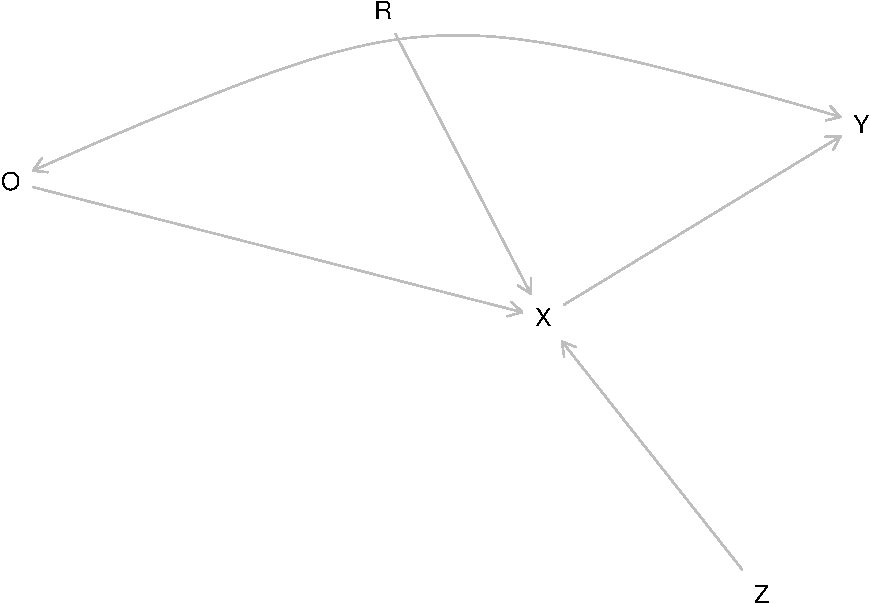
\includegraphics{ii_files/figure-latex/appcombexpob-1} 

}

\caption{A model that nests an observational and an experimental study. The treatment $X$ either takes on the observational value $O$, or the assigned values $Z$, depending on whether or not the case has been randomized, $R$.}\label{fig:appcombexpob}
\end{figure}

Now, let us imagine true parameter values such that \(X\) has a \(0.2\) average effect on \(Y\). However, the effect is different for those who are selected into treatment in an observational setting: it is positive (\(0.6\)) for cases in which \(X=1\) under observational assignment, but negative (\(-0.2\)) for cases in which \(X=0\) under observational assignment. (See appendix for complete specification.)

When we use the model to analyze the data, we will start with flat priors on the causal types.

The implied true values for the estimands of interest, and our priors on those estimands, are displayed in Table \ref{tab:fusionestimands}.

\begin{table}

\caption{\label{tab:fusionestimands}Estimands in different sites}
\centering
\begin{tabular}[t]{lllrr}
\toprule
Query & Given & Using & mean & sd\\
\midrule
\cellcolor{gray!6}{ATE} & \cellcolor{gray!6}{-} & \cellcolor{gray!6}{parameters} & \cellcolor{gray!6}{0.20} & \cellcolor{gray!6}{}\\
ATE & - & priors & -0.01 & 0.26\\
\cellcolor{gray!6}{ATE} & \cellcolor{gray!6}{R==0} & \cellcolor{gray!6}{parameters} & \cellcolor{gray!6}{0.20} & \cellcolor{gray!6}{}\\
ATE & R==0 & priors & -0.01 & 0.26\\
\cellcolor{gray!6}{ATE} & \cellcolor{gray!6}{R==1} & \cellcolor{gray!6}{parameters} & \cellcolor{gray!6}{0.20} & \cellcolor{gray!6}{}\\
\addlinespace
ATE & R==1 & priors & -0.01 & 0.26\\
\bottomrule
\end{tabular}
\end{table}

Now, we generate data from the model, using the posited ``true'' parameter values, and then update the model using these data.

We begin by analyzing just the observational data (cases where \(R=0\)) and display the results in Table \ref{tab:fusiondim}. Recall that the true average effect of \(X\) on \(Y\) is \(0.2\). Naive analysis of the observational data, taking a simple difference in means between the \(X=0\) and \(X=1\) cases, yields a strongly upwardly biased estimate of that effect, of 0.0806.

\begin{table}

\caption{\label{tab:fusiondim}Inferences on the ATE from differences in means}
\centering
\begin{tabular}[t]{lrrrrrrr}
\toprule
  & Estimate & Std. Error & t value & Pr(>|t|) & CI Lower & CI Upper & DF\\
\midrule
\cellcolor{gray!6}{X} & \cellcolor{gray!6}{0.831} & \cellcolor{gray!6}{0.027} & \cellcolor{gray!6}{30.37} & \cellcolor{gray!6}{0} & \cellcolor{gray!6}{0.777} & \cellcolor{gray!6}{0.885} & \cellcolor{gray!6}{188}\\
\bottomrule
\end{tabular}
\end{table}

In contrast, when we use \texttt{CausalQueries} to update on the full causal model and use both the experimental and observational data, we get the much more accurate results shown in Table \ref{tab:fusionCQ}. Moving down the rows, we show here the estimate of the unconditional \(ATE\), the estimate for the observational context (\(R=0\)), and the estimate for the experimental context (\(R=1\)). Unsurprisingly, the estimates are identical across all three settings since, in the model, \(R\) is \(d\)-separated from \(Y\) by \(X\), which is observed. And, as we see, the posterior means are very close to the right answer of \(0.2\).

\begin{table}

\caption{\label{tab:fusionCQ}Estimates on the ATE for observational ($R=0$) and experimental ($R=1$) set.}
\centering
\begin{tabular}[t]{lllrr}
\toprule
Query & Given & Using & mean & sd\\
\midrule
\cellcolor{gray!6}{ATE} & \cellcolor{gray!6}{-} & \cellcolor{gray!6}{posteriors} & \cellcolor{gray!6}{0.22} & \cellcolor{gray!6}{0.029}\\
ATE & R==0 & posteriors & 0.22 & 0.029\\
\cellcolor{gray!6}{ATE} & \cellcolor{gray!6}{R==1} & \cellcolor{gray!6}{posteriors} & \cellcolor{gray!6}{0.22} & \cellcolor{gray!6}{0.029}\\
\bottomrule
\end{tabular}
\end{table}

Since the model used both the experimental and the observational data, we might wonder from where the leverage derived: did the observational data improve our estimates of the average treatment effect, or do our inferences emerge strictly from the experimental data? In the appendix, we show results when we updating using experimental data only.
Comparing the two sets of results, we find there that we do indeed get a tightening of posterior variance and a more accurate result when we use both the observational and experimental data, but the experimental data alone are quite powerful, as we should expect for an estimate of the \(ATE\). The observational data do not add a great deal to an \(ATE\) estimate, and the gains from observational data would be smaller still (and the experimental results even more accurate) if the experimental sample were larger.

However, what we can learn about uniquely from this model and the combined observational and experimental data is \emph{heterogeneity} in effects between those that are in treatment and those that are in control \emph{in the observational} setting. In Table \ref{tab:combexpobsattatc}, we display the results of \(ATT\) and \(ATC\) queries of the updated model. In the first two rows, we see that, in the experimental setting, the average effect of \(X\) on \(Y\) is the same on both the treated and control groups, exactly as we would expect under random assignment. In the third row, we see the estimate of \(X\)'s average effect for those assigned ``by nature'' to the control group in the observational setting, extracting a result close to the ``true'' value of \(-0.2\). The final row shows our estimate of the treatment effect for those who are selected into treatment in the observational setting, again getting close to the answer implied by the underlying data-generating process (\(0.6\)).

\begin{table}

\caption{\label{tab:combexpobsattatc}Effects of $X$ conditional on $X$ for units that were randomly assigned or not.  Effects of $X$ do not depend on $X$ in the experimental group, but they do in the observational group becuase of seld selection. }
\centering
\begin{tabular}[t]{lllrr}
\toprule
Query & Given & Using & mean & sd\\
\midrule
\cellcolor{gray!6}{ATE} & \cellcolor{gray!6}{R==1 \& X==0} & \cellcolor{gray!6}{posteriors} & \cellcolor{gray!6}{0.220} & \cellcolor{gray!6}{0.029}\\
ATE & R==1 \& X==1 & posteriors & 0.220 & 0.029\\
\cellcolor{gray!6}{ATE} & \cellcolor{gray!6}{R==0 \& X==0} & \cellcolor{gray!6}{posteriors} & \cellcolor{gray!6}{-0.159} & \cellcolor{gray!6}{0.025}\\
ATE & R==0 \& X==1 & posteriors & 0.627 & 0.044\\
\bottomrule
\end{tabular}
\end{table}

We can learn nothing about the observational \(ATT\) or \(ATC\) from the experimental data alone, where there \(ATT\) and \(ATC\) are the same quantity. And in the observational data alone, we are hobbled by confounding of unknown direction and size. What the mixed model and data, in effect, are able to do is (a) learn about the \(ATE\) experimental data, (b) use inferences on the \(ATE\) to separate true effects from confounding in the observational data and thus learn about the direction and size of the confounding in those data, and (c) estimate the treatment effect for the \(X=0\) group and for the \(X=1\) group, respectively, in the observational data \emph{using} knowledge about confounding in these data. By mixing the experimental and observational data, we can learn about how the treatment has affected those units that, in the ``real'' world of the observational setting, selected into treatment \emph{and} about how the treatment \emph{would} affect those that selected into control.

The numbers in our toy example, while purely notional, can help us see why the observational \(ATT\) and \(ATC\) might be of great interest to decision makers where strong causal heterogeneity is a possibility. Based on the experimental data alone, we might conclude that the policy that makes \(X=1\) available is a good bet, given its positive \(ATE\) (assuming, of course, that \(Y=1\) is a valued outcome). And, of course, the observational data alone would not allow us to confidently conclude otherwise. What the integrated analysis reveals, however, is that \(X\) in fact has a \emph{negative} mean effect on those who would be most likely to take up the treatment. The strong positive effect for the control strongly shapes the experimental results but will go unrealized in the real world.
In a similar vein, these estimates can aid causal explanation. Seeing the positive \(ATE\) might lead us to infer that most of the \(X=1, Y=1\) cases we observe in the world are ones in which \(X=1\) caused \(Y=1\). The observational \(ATT\) estimates point in a very different direction, however, indicating that these are cases in which \(X\) is least likely to have a positive effect and, thus, where \(Y=1\) was most likely generated by some other cause.

We note that the results here relate to the LATE theorem \citep{angrist1995identification}. Imagine using data only on (a) the experimental group in control and (b) the observational group, some of whom are in treatment. We can conceptualize our design as one in which the observational group are ``encouraged'' to take up treatment, allowing us to estimate the effect for the ``compliers'' in the observational setting: those that self-select into treatment. Conversely, we could use data only on (a) the experimental group in treatment and (b) the observational group, some of whom are in control. This is a design in which the observational group are ``encouraged'' to take the control condition, allowing us to estimate the effect for the ``compliers'' in this group (those that self select into control).

\hypertarget{transportation-of-findings-across-contexts}{%
\section{Transportation of findings across contexts}\label{transportation-of-findings-across-contexts}}

In some circumstances, we study the effect of \(X\) on \(Y\) in one context (a country, region, or time period, for instance) and then want to make inferences about these effects in another context (say, another country, region, or time period). We may face the challenge that effects are heterogeneous, and that conditions that vary across contexts may be related to treatment assignment, to outcomes, and to selection into the sample. For example, we might study the relationship between inequality and democratization in low-income countries and then want to know how those effects travel to middle-income settings. However, the level of income may have implications jointly for the level of inequality and for how likely inequality is to generate regime change, meaning that causal effects uncovered in the first context cannot be assumed to operate in the second context.

This is the problem studied by \citet{pearl2014external}. In particular, \citet{pearl2014external} show for which nodes data are needed in order to ``licence'' external claims, given a model.

We illustrate with a simple model in which an observable confounder has a different distribution across contexts. In the model drawn in Figure \ref{fig:extval}, \(Context\) determines the distribution of the confounder, \(W\). We set a restriction such that the value of \(W\) in Context 1 is never less than the value of \(W\) in Context 0; our priors are otherwise flat over the remaining nodal types in the model.

\begin{figure}

{\centering 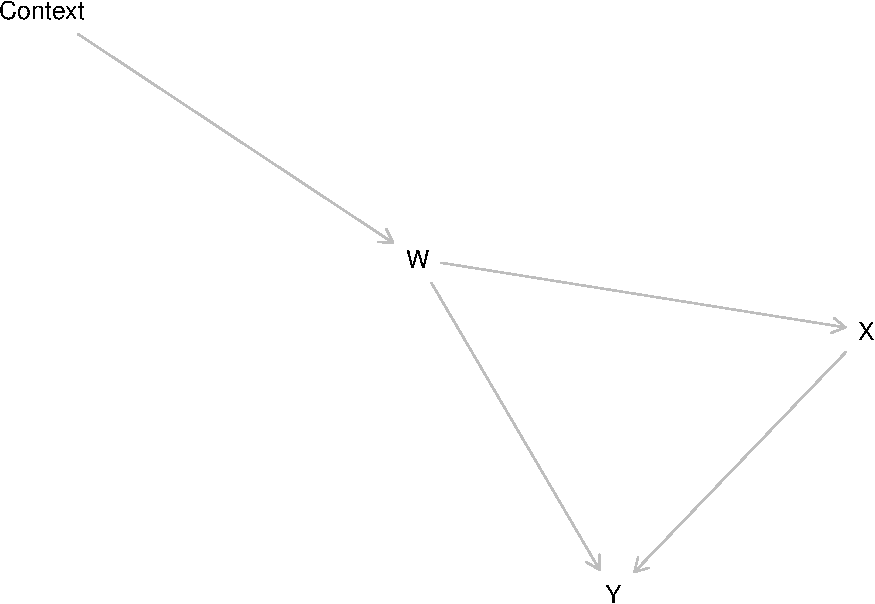
\includegraphics{ii_files/figure-latex/extval-1} 

}

\caption{Extrapolation when confounders have different distributions across cases.}\label{fig:extval}
\end{figure}

\begin{table}

\caption{\label{tab:appev2}Priors and true values (parameters) for three estimands: the frequency of $W$, the effect of $X$ on $Y$, and the effect conditional on $W=1$}
\centering
\begin{tabular}[t]{lllrr}
\toprule
Query & Given & Using & mean & sd\\
\midrule
\cellcolor{gray!6}{Incidence} & \cellcolor{gray!6}{Context==0} & \cellcolor{gray!6}{priors} & \cellcolor{gray!6}{0.332} & \cellcolor{gray!6}{0.231}\\
Incidence & Context==0 & parameters & 0.333 & \\
\cellcolor{gray!6}{Incidence} & \cellcolor{gray!6}{Context==1} & \cellcolor{gray!6}{priors} & \cellcolor{gray!6}{0.666} & \cellcolor{gray!6}{0.234}\\
Incidence & Context==1 & parameters & 0.667 & \\
\cellcolor{gray!6}{ATE} & \cellcolor{gray!6}{Context==0} & \cellcolor{gray!6}{priors} & \cellcolor{gray!6}{0.001} & \cellcolor{gray!6}{0.138}\\
\addlinespace
ATE & Context==0 & parameters & 0.333 & \\
\cellcolor{gray!6}{ATE} & \cellcolor{gray!6}{Context==1} & \cellcolor{gray!6}{priors} & \cellcolor{gray!6}{0.000} & \cellcolor{gray!6}{0.140}\\
ATE & Context==1 & parameters & 0.573 & \\
\cellcolor{gray!6}{CATE} & \cellcolor{gray!6}{Context==0} & \cellcolor{gray!6}{priors} & \cellcolor{gray!6}{0.001} & \cellcolor{gray!6}{0.169}\\
CATE & Context==0 & parameters & 0.812 & \\
\addlinespace
\cellcolor{gray!6}{CATE} & \cellcolor{gray!6}{Context==1} & \cellcolor{gray!6}{priors} & \cellcolor{gray!6}{0.001} & \cellcolor{gray!6}{0.169}\\
CATE & Context==1 & parameters & 0.812 & \\
\bottomrule
\end{tabular}
\end{table}

We show priors and true values for the estimands (drawn from the parameters) in Table \ref{tab:appev2}. We see that the incidence of \(W=1\) is higher in Context 1 than in Context 0, both in our priors and in the ``truth'' posited by the assigned parameter values. The ``true'' \(ATE\) of \(X\) on \(Y\) is also higher in Context 1, though this is not reflected in our priors. The average treatment effect conditional on \(W\) is the same in both contexts, whether we work from priors or assigned parameter values, as it must be given the model. That is, in this model the \(ATE\) varies conditional on \(W\) --- and it varies conditional \emph{only} on \(W\).

We now update the model using data from one context and then see if we can transport those findings to the other context. Specifically, we update using data on \(X, Y,\) and \(W\) from Context 0. We then use the updated beliefs to draw inferences about Context 1, using data \emph{only} on \(W\) from Context 1. In Table \ref{tab:appev3}, we show our posteriors on the queries of interest as compared to the truth, given the parameter values.

\begin{table}

\caption{\label{tab:appev3}Extrapolation when two sites differ on $W$ and $W$ is observable in both contexts}
\centering
\begin{tabular}[t]{lllrr}
\toprule
Query & Given & Using & mean & sd\\
\midrule
\cellcolor{gray!6}{Incidence} & \cellcolor{gray!6}{Context==0} & \cellcolor{gray!6}{posteriors} & \cellcolor{gray!6}{0.324} & \cellcolor{gray!6}{0.007}\\
Incidence & Context==0 & parameters & 0.333 & \\
\cellcolor{gray!6}{Incidence} & \cellcolor{gray!6}{Context==1} & \cellcolor{gray!6}{posteriors} & \cellcolor{gray!6}{0.676} & \cellcolor{gray!6}{0.007}\\
Incidence & Context==1 & parameters & 0.667 & \\
\cellcolor{gray!6}{ATE} & \cellcolor{gray!6}{Context==0} & \cellcolor{gray!6}{posteriors} & \cellcolor{gray!6}{0.330} & \cellcolor{gray!6}{0.011}\\
\addlinespace
ATE & Context==0 & parameters & 0.333 & \\
\cellcolor{gray!6}{ATE} & \cellcolor{gray!6}{Context==1} & \cellcolor{gray!6}{posteriors} & \cellcolor{gray!6}{0.578} & \cellcolor{gray!6}{0.009}\\
ATE & Context==1 & parameters & 0.573 & \\
\cellcolor{gray!6}{CATE} & \cellcolor{gray!6}{Context==0} & \cellcolor{gray!6}{posteriors} & \cellcolor{gray!6}{0.807} & \cellcolor{gray!6}{0.009}\\
CATE & Context==0 & parameters & 0.812 & \\
\addlinespace
\cellcolor{gray!6}{CATE} & \cellcolor{gray!6}{Context==1} & \cellcolor{gray!6}{posteriors} & \cellcolor{gray!6}{0.807} & \cellcolor{gray!6}{0.009}\\
CATE & Context==1 & parameters & 0.812 & \\
\bottomrule
\end{tabular}
\end{table}

By comparing the \(ATE\) estimates using our posteriors and the estimates using the assigned parameter values, we see that we have done well in recovering the effects, \emph{both} for the context we studied (i.e., in which we observed \(X\) and \(Y\)) and for the context we did not study. We can think of the learning here as akin to post-stratification. We have learned from observing \(X, Y\), and \(W\) in Context 0 how \(X\)'s effect depends on \(W\). Then we use those updated beliefs when confronted with a new value of \(W\) in Context 1 to form a belief about \(X\)'s effect in this second context. Of course, getting the right answer from this procedure depends, as always, on starting with the correct model.

We can also see, in Table \ref{tab:appev4}, what would have happened if we had attempted to make the extrapolation to Context 1 without data on \(W\) in that context. We would get the wrong answer for Context 1, though we would also report greater posterior variance. The higher posterior variance here captures the fact that we know things could be different in Context 1, but we don't know in what way they are different.

\begin{table}

\caption{\label{tab:appev4}Extrapolation when two contexts differ on $W$ and $W$ is not observable in target context}
\centering
\begin{tabular}[t]{lllrr}
\toprule
Query & Given & Using & mean & sd\\
\midrule
\cellcolor{gray!6}{Incidence} & \cellcolor{gray!6}{Context==0} & \cellcolor{gray!6}{posteriors} & \cellcolor{gray!6}{0.329} & \cellcolor{gray!6}{0.007}\\
Incidence & Context==0 & parameters & 0.333 & \\
\cellcolor{gray!6}{Incidence} & \cellcolor{gray!6}{Context==1} & \cellcolor{gray!6}{posteriors} & \cellcolor{gray!6}{0.667} & \cellcolor{gray!6}{0.007}\\
Incidence & Context==1 & parameters & 0.667 & \\
\cellcolor{gray!6}{ATE} & \cellcolor{gray!6}{Context==0} & \cellcolor{gray!6}{posteriors} & \cellcolor{gray!6}{0.314} & \cellcolor{gray!6}{0.012}\\
\addlinespace
ATE & Context==0 & parameters & 0.333 & \\
\cellcolor{gray!6}{ATE} & \cellcolor{gray!6}{Context==1} & \cellcolor{gray!6}{posteriors} & \cellcolor{gray!6}{0.560} & \cellcolor{gray!6}{0.009}\\
ATE & Context==1 & parameters & 0.573 & \\
\cellcolor{gray!6}{CATE} & \cellcolor{gray!6}{Context==0} & \cellcolor{gray!6}{posteriors} & \cellcolor{gray!6}{0.801} & \cellcolor{gray!6}{0.009}\\
CATE & Context==0 & parameters & 0.812 & \\
\addlinespace
\cellcolor{gray!6}{CATE} & \cellcolor{gray!6}{Context==1} & \cellcolor{gray!6}{posteriors} & \cellcolor{gray!6}{0.801} & \cellcolor{gray!6}{0.009}\\
CATE & Context==1 & parameters & 0.812 & \\
\bottomrule
\end{tabular}
\end{table}

\hypertarget{multilevel-models-meta-analysis}{%
\section{Multilevel models, meta-analysis}\label{multilevel-models-meta-analysis}}

A key idea in Bayesian meta-analysis is that when you analyze multiple studies together you learn not only about common processes that give rise to the different results seen in different sites, but you also learn more about each study from seeing the other studies.

A classic setup is provided in \citet{gelman2013bayesian}, in which we have access to estimates of effects and uncertainty in eight sites (schools), \((b_j, se_j)_{j \in \{1,2,\dots,8\}}\). To integrate learning across these studies we employ a ``hierarchical model''
that treats each \(b_j\) as a draw from distribution \(N(\beta_j, se_j)\) (and, in turn treats each \(\beta_j\) is a draw from distribution \(N(\beta, \sigma)\)). In that setup we want to learn about the superpopulation parameters \(\beta, \sigma\), but we also get to learn more about the study level effects \((\beta_j)_{j \in \{1,2,\dots,8\}}\) by studying them jointly.

A hierarchical model like this allows us to think about the populations in our study sites as themselves drawn from a larger population (``superpopulation'') of settings. And, crucially, it allows us in turn to use data in the study sites to learn about that broader superpopulation of settings.

Although often used in the context of linear models with parameters for average causal effects, this logic works just as well with the kinds of causal models we have been using in this book.

Let's review how our analytic setup has worked so far. At each node in a causal model, we conceptualize a given case as having a particular nodal type. The case's nodal type is drawn from a distribution of nodal types in the population of cases from which this case has been drawn. When we do process tracing, we consider that population-level distribution to be a set of fixed shares of nodal types in the population: say, for node \(Y\), we might believe that half the cases in the population are \(\lambda^Y_{01}\), a quarter are \(\lambda^Y_{00}\), and a quarter are \(\lambda^Y_{11}\). We then use data from the case to update on the case's nodal types (or on the combination of nodal types that correspond to some case-level query), given the population-level shares.

When we engage in population-level inference, we begin with \emph{uncertainty} about the population-level shares of types, and we express our prior beliefs about those shares as a Dirichlet \emph{distribution}. So, for instance, our beliefs might be centered around a \(\lambda^Y_{01}=0.5, \lambda^Y_{00}=0.25, \lambda^Y_{11}=0.25\) breakdown of shares in the population; and we also express some degree of uncertainty about what the breakdown is. Now, when we analyze data on some number of cases, we can update both on those cases' types and on our beliefs about the distribution of types in the population -- perhaps shifting toward a higher share of \(\lambda^Y_{01}\)'s (and with a change in the distribution's variance).

We can also, as in the last section, build a model in which there are multiple settings, possibly differing on some population-level characteristic. Fundamentally, however, the setup in the last section still involved population-level inference in that we were assuming that the \emph{type shares} (\(\lambda\) values) are the same across settings. The settings might differ in the value of a moderating variable, but they do not differ in the shares of cases that \emph{would} respond in any given way to the moderator (and other causal conditions). The data allow us to update on what those common, cross-setting type proportions are.

When we build a hierarchical model, each case is still understood as being embedded within a population: our cases might be citizens, say, each embedded within a country. The key difference from population-level inference is that we now conceive of there being \emph{multiple} populations -- say, multiple countries -- each drawn from a population of populations, or superpopulation. Now, we think of each population (country) as having its own set of type shares for each node. And we think of each country's type shares as being drawn from a Dirichlet distribution of type shares (for each node) that lives at the superpopulation level. Moreover, we are \emph{uncertain} about what that distribution at the superpopulation level \emph{is}. We uncertain around what type proportions the superpopulation-level distribution is centered, and we are uncertain about how dispersed this distribution is. While the distribution's central tendency will be related to the mean type shares for countries, its variance will determine the degree of \emph{heterogeneity} across countries in their type shares.

To summarize, in population-level inference, we express uncertainty about the population's type shares with a Dirichlet prior, at the population level, on which we update. In the hierarchical setting, we are uncertain both about the population-level type shares and the superpopulation Dirichlet from which each node's type shares are drawn. We express our uncertainty about each superpopulation Dirichlet by positing a prior distribution over the Dirichlet's alpha parameters.

Now, when we observe data on citizens within countries, we can update our beliefs about types fora the particular citizens we observe, about type shares in the population of citizens within each country that we study, \emph{and} on the parameters of the Dirichlet distribution from which population shares have been drawn. In updating on the last of these, we are learning not just about the countries we observe but also about those we do not directly observe.

We illustrate with a simulation using a simple \(X,Y\) model. We imagine that we are studying the \(X \rightarrow Y\) relationship in \texttt{n} countries. Each country has a parameter distribution drawn from common Dirichelets. We start off with flat priors over the alpha arguments of the superpopulation Dirichlets.

We assign a particular true set of superpopulation parameter values that, for the analytic exercise, is treated as unknown and that we would like to recover. In this true world, the probability of assignment to \(X=1\) is .4, and the average treatment effect is .1. Using these true parameter values, we simulate \(X, Y\) data for \(n=8\) countries.

\begin{figure}

{\centering 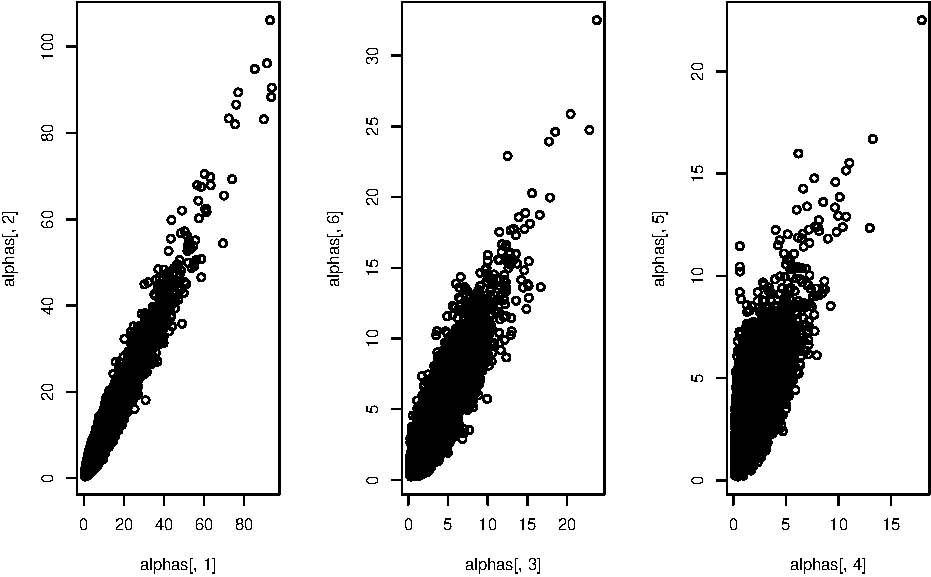
\includegraphics{ii_files/figure-latex/plotalphas-1} 

}

\caption{Joint distributions over alpha parameters.}\label{fig:plotalphas}
\end{figure}

In Figure \ref{fig:plotalphas}, we graph our posterior beliefs about the superpopulation parameters. We do this by plotting two alpha parameters against each other at a time. In the first panel, we plot the alphas for \(X=0\) and \(X=1\). In the next panel, we plot the alpha's corresponding to \(c\) types against those corresponding to \(d\) types. And in the third panel we plot the alpha's corresponding to \(a\) types against those corresponding to \(b\) types.

As we can see, each distribution falls roughly along a diagonal. Probability mass located further up the diagonal represents worlds in which the superpopulation Dirichlet distribution of type shares is relatively low in variance. Thus, the more that our posterior beliefs are concentrated toward a graph's northeast corner, the lower the heterogeneity we have inferred there to be in the relevant type shares across countries. Meanwhile, the dispersion of probability mass \emph{away} from the diagonal represents greater posterior \emph{uncertainty} about the heterogeneity across countries, arising from greater variance about the posterior distribution of the alphas.

We can think of a concentration parameter here that is operationalized as the sum of the \(\alpha^j\) terms for a node, \(j\), with a higher value representing lower overall heterogeneity.

\begin{figure}

{\centering 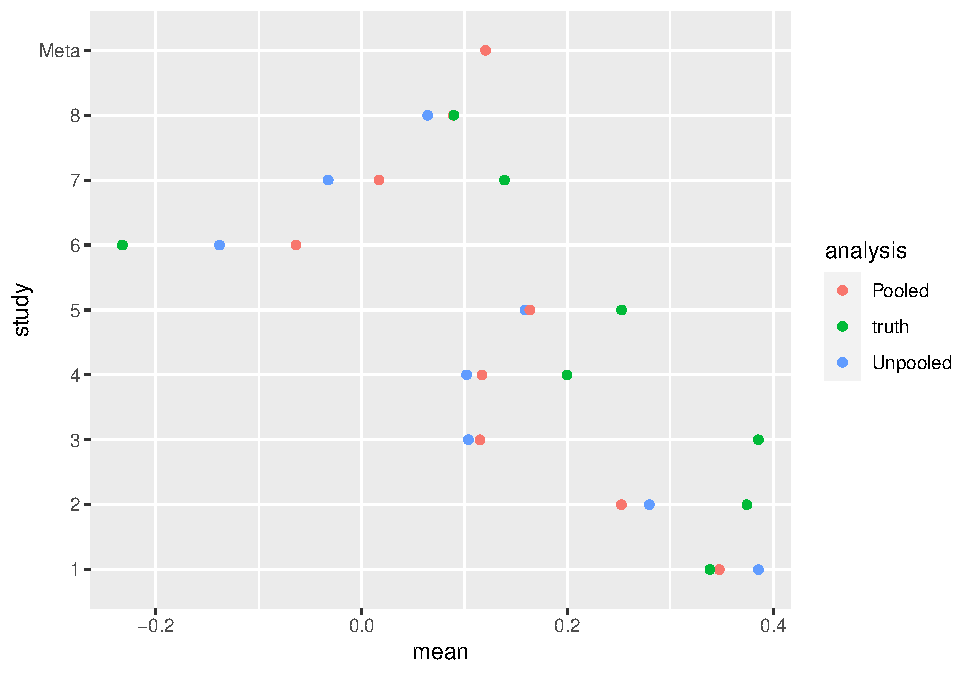
\includegraphics{ii_files/figure-latex/metaplot-1} 

}

\caption{Updating on study level parameters from integrated analyses. }\label{fig:metaplot}
\end{figure}

In Figure \ref{fig:metaplot} we turn to the causal query of interest and show a comparison of three \(ATE\) estimates for each country: in blue, we show the unpooled estimate, or the estimate we get for each country using only data from that country; in red, we see the pooled estimates, or the estimate we get for each country using data from \emph{all} countries to inform that country's parameter estimates; and in black, we plot the truth as posited for this simulation. As we can see, the pooled estimates are all closer to the center than the unpooled estimates: this is because we are effectively using data from all countries to discount extreme features of the data observed in a given country. Put differently, the pooled data serve the function of a prior when it comes to drawing inferences about a single country: our inference is a compromise between the data from that country and the beliefs we have formed from the pooled data. We can also see that, for most countries, the pooling helps: the regularization provided by the pooling gives us an estimate closer to the truth for most of the settings.

\hypertarget{clue}{%
\chapter{Clue Selection as a Decision Problem}\label{clue}}

\begin{headerbox}
We draw out the implications of the causal model approach for clue-selection strategies. We demonstrate procedures for assessing which clues minimize expected variance and how to construct an optimal decision tree for determining a clue gathering strategy.

\end{headerbox}

We now mobilize the causal models framework for the purposes of making research-design choices. We start with the problem of clue-selection: determining which qualitative data to gather on a case. Evidently it makes sense to gather clues that have large probative value, but whether or not a given clue will have probative value depends on the model we are working with and the question we are asking. As we will also see, a clue's informativeness can depend on what other clues have already been collected. Finding out that the butler had no motive may be informative for the claim that he is innocent, but it may not be useful if we already know that he had no opportunity.

We have already provided some insight into the problem in Chapter \ref{pt}, where we showed how relations of \(d-\)connection can tell us when a clue is \emph{possibly} informative about a query. In this chapter, we go further to show how we can use our causal model to figure out which clues and clue-selection strategies are likely to be \emph{most} informative about the query we seek to address.

\hypertarget{a-model-informed-approach-to-clue-selection}{%
\section{A model-informed approach to clue-selection}\label{a-model-informed-approach-to-clue-selection}}

The representation of inference problems as one of querying a Bayesian model points to a relatively simple method for selecting the most informative clues for collection. Consider, first, a situation in which one can invest in collecting various forms of evidence on a case and wants to know the expected probative value of all possible collections of evidence that one could gather.

We can assess alternative strategies through the following procedure:

\begin{enumerate}
\def\labelenumi{\arabic{enumi}.}
\tightlist
\item
  Define the model.
\item
  Define a query on the model.
\item
  Define a data strategy: a set of clues for which one might search (e.g., observe the value of \(Y\)).
\item
  Given prior data, figure out the probability of different realizations of the new data.
\item
  For each possible realization, calculate the posterior variance.
\item
  Calculate the \emph{expected} posterior variance for the data strategy by taking a weighted average of the variances arising from the different data realizations, with weights given by the probability of observing the data-realization in question.
\item
  Repeat steps 3-4 for different data strategies that we wish to compare.
\end{enumerate}

This procedure then allows us to choose the clue strategy with the lowest expected posterior variance.

A still more sophisticated strategy would, for multiple clues, take sequence into account: it would tell us which clues to search for later in the process given the realization of clues sought earlier. The path-dependence of clue selection arises from the possibility that the informativeness of a clue may depend on the value of other nodes in the model. A given clue \(K_2\), for instance, may be informative if another clue \(K_1\) has the value of 1 but not if it has the value 0.

We provide tools for both of these approaches and illustrate them below for both the running example and the democracy application.

\hypertarget{clue-selection-with-a-simple-example}{%
\subsection{Clue selection with a simple example}\label{clue-selection-with-a-simple-example}}

We first spell out how this works using a hypothetical example and then explore further using our democratization model.

Consider a model of government survival in office in which retaining office depends on not being perceived as corrupt by the public, graphed in Figure \ref{fig:running}. We take two conditions as being exogenous in this model. First, a country may or may not have a free press (\(X\)). Second, the country's government may or may not be sensitive to public opinion (\(S\)).\footnote{Government sensitivity here can be thought of as government sophistication (does it take the actions of others into account when making decisions?) or as a matter of preferences (does it have a dominant strategy to engage in corruption?).} In terms of causal relations, we then allow that the government's decision about whether to engage in corruption (\(C=1\)) may depend on whether the government is sensitive to public opinion and whether there is a free press (that might reveal that corruption). Moreover, we allow that whether the press will report on the corruption (\(R=1\)) may depend on whether there is government corruption and whether the press is free. Finally, whether the government will be removed from office (\(Y=1\)) may depend on whether it has acted corruptly and whether this gets reported in the press.

\begin{figure}

{\centering 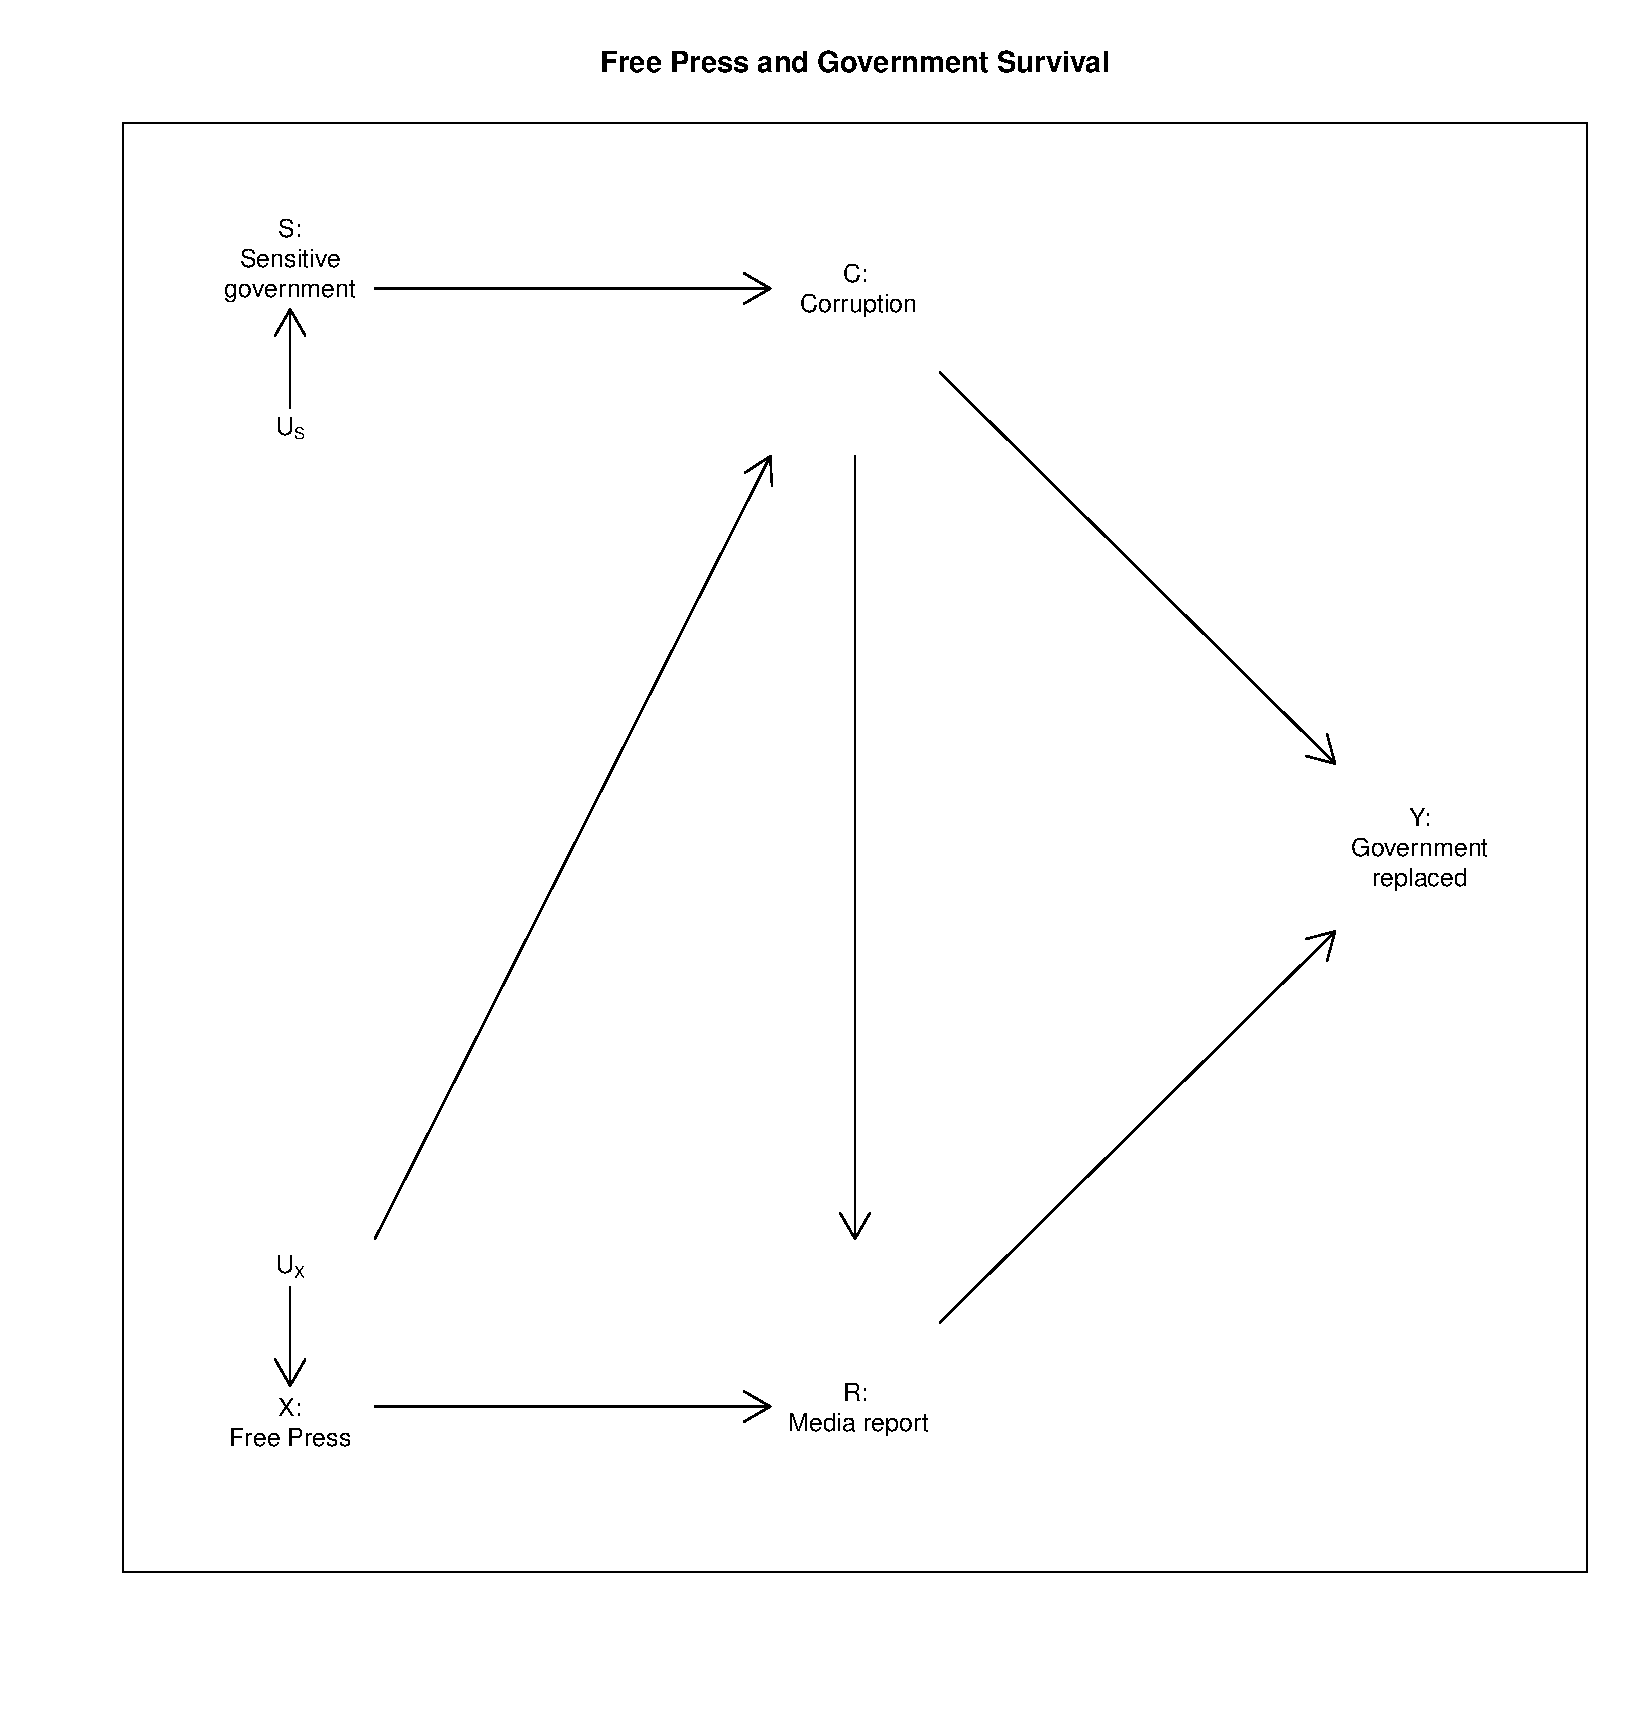
\includegraphics[width=0.7\linewidth]{ii_files/figure-latex/running-1} 

}

\caption{The figure shows a simple causal model. $S$ and $X$ are stochastic, $C$ and $R$ have only two possible nodal types each, $Y=1$ if and only if $C$ and $R$ are both 1.}\label{fig:running}
\end{figure}

To simplify the illustration we work with a highly restricted version of this model. At node \(C\), we allow only two types: either corruption is always present (\(\theta^C_{1111}\)) or corruption is always present except when there is both a free press (\(X=1\)) and sensitivity to public opinion (\(S=1\)) (\(\theta^C_{1110}\)). At \(R\), we allow only for \(\theta^R_{0001}\) and \(\theta^R_{0000}\): the possibility that there is reporting on corruption if and only if there is corruption and a free press, and the possibility that there is never reporting on corruption. Finally, at \(Y\), we restrict to just one nodal type, \(\theta^Y_{0001}\): the government will remain in office unless there is both corruption (\(C=1\)) and reporting on corruption (\(R=1\)).

To summarize the intuition, then, governments will fall only if there is both corruption and reporting on corruption. We are uncertain whether or not corruption is always present; but if corruption is ever absent, it can only be because there exists both a free press and a government that cares about public opinion. We are also uncertain whether or not media reporting on corruption is always absent; but if it is ever present, it can only be because there is both corruption and a free press. One implication is that governments that are sensitive to public opinion will never fall because they will always eschew corruption when a free press---the only mechanism that can generate reporting on corruption---is present. In turn, the presence of a free press can only matter for government survival if governments are \emph{not} sensitive and thus do not strategically adjust their behavior in response to the risk of reporting.

Suppose now that our query is whether \(X\) has a positive effect on \(Y\). Using this model we can ask how likely different data realizations are and what we would infer about our query from each possible data realization, given existing data. We illustrate for a situation in which we already know that \(Y=0\).

Application of the function \texttt{conditional\_inferences} produces a matrix with the results. We reproduce these as Table \ref{tab:showstrats5xx}. The first five columns of Table \ref{tab:showstrats5xx} define the data realizations. The matrix includes all combinations of possible realized values for all available clue strategies given that we have already observed \(Y=0\). Note that since we can already infer that \(R=0\) we omit strategies that seek data on \(R\). A ``0'' or ``1'' represents the observed value for a node that we have chosen to observe while ``?'' indicates that a node is not observed under the given strategy. Thus, for instance, in the first 5 rows we are collecting data on all nodes. In the next three rows, we have sought data on all nodes except \(S\).

We also indicate the probability of each realization given the srtategy, the inference we would make from each data-realization---that is, the posterior probability that \(X\) has a positive effect on \(Y\), given that \(Y=0\)---and the posterior variance.

The figures show all combinations of possible realized values for all available clue strategies given that we have already observed \(Y=0\). A ``0'' or ``1'' represents the observed value for a node that we have chosen to observe while \(?\) under a node indicates that that node is not observed under the given strategy.

\begin{table}

\caption{\label{tab:showstrats5xx}Inferences given different data patterns, with observations on some or all nodes.}
\centering
\begin{tabular}[t]{lllllrrrr}
\toprule
strategy & S & X & C & R & Y & prob & posterior & variance\\
\midrule
\cellcolor{gray!6}{SXC} & \cellcolor{gray!6}{1} & \cellcolor{gray!6}{1} & \cellcolor{gray!6}{0} & \cellcolor{gray!6}{0} & \cellcolor{gray!6}{0} & \cellcolor{gray!6}{0.154} & \cellcolor{gray!6}{0.000} & \cellcolor{gray!6}{0.000}\\
SXC & 0 & 0 & 1 & 0 & 0 & 0.308 & 0.500 & 0.250\\
\cellcolor{gray!6}{SXC} & \cellcolor{gray!6}{1} & \cellcolor{gray!6}{0} & \cellcolor{gray!6}{1} & \cellcolor{gray!6}{0} & \cellcolor{gray!6}{0} & \cellcolor{gray!6}{0.308} & \cellcolor{gray!6}{0.250} & \cellcolor{gray!6}{0.188}\\
SXC & 0 & 1 & 1 & 0 & 0 & 0.154 & 0.000 & 0.000\\
\cellcolor{gray!6}{SXC} & \cellcolor{gray!6}{1} & \cellcolor{gray!6}{1} & \cellcolor{gray!6}{1} & \cellcolor{gray!6}{0} & \cellcolor{gray!6}{0} & \cellcolor{gray!6}{0.077} & \cellcolor{gray!6}{0.000} & \cellcolor{gray!6}{0.000}\\
\addlinespace
XC & ? & 1 & 0 & 0 & 0 & 0.154 & 0.000 & 0.000\\
\cellcolor{gray!6}{XC} & \cellcolor{gray!6}{?} & \cellcolor{gray!6}{0} & \cellcolor{gray!6}{1} & \cellcolor{gray!6}{0} & \cellcolor{gray!6}{0} & \cellcolor{gray!6}{0.615} & \cellcolor{gray!6}{0.375} & \cellcolor{gray!6}{0.234}\\
XC & ? & 1 & 1 & 0 & 0 & 0.231 & 0.000 & 0.000\\
\cellcolor{gray!6}{SC} & \cellcolor{gray!6}{1} & \cellcolor{gray!6}{?} & \cellcolor{gray!6}{0} & \cellcolor{gray!6}{0} & \cellcolor{gray!6}{0} & \cellcolor{gray!6}{0.154} & \cellcolor{gray!6}{0.000} & \cellcolor{gray!6}{0.000}\\
SC & 0 & ? & 1 & 0 & 0 & 0.462 & 0.333 & 0.222\\
\addlinespace
\cellcolor{gray!6}{SC} & \cellcolor{gray!6}{1} & \cellcolor{gray!6}{?} & \cellcolor{gray!6}{1} & \cellcolor{gray!6}{0} & \cellcolor{gray!6}{0} & \cellcolor{gray!6}{0.385} & \cellcolor{gray!6}{0.200} & \cellcolor{gray!6}{0.160}\\
SX & 0 & 0 & ? & 0 & 0 & 0.308 & 0.500 & 0.250\\
\cellcolor{gray!6}{SX} & \cellcolor{gray!6}{1} & \cellcolor{gray!6}{0} & \cellcolor{gray!6}{?} & \cellcolor{gray!6}{0} & \cellcolor{gray!6}{0} & \cellcolor{gray!6}{0.308} & \cellcolor{gray!6}{0.250} & \cellcolor{gray!6}{0.188}\\
SX & 0 & 1 & ? & 0 & 0 & 0.154 & 0.000 & 0.000\\
\cellcolor{gray!6}{SX} & \cellcolor{gray!6}{1} & \cellcolor{gray!6}{1} & \cellcolor{gray!6}{?} & \cellcolor{gray!6}{0} & \cellcolor{gray!6}{0} & \cellcolor{gray!6}{0.231} & \cellcolor{gray!6}{0.000} & \cellcolor{gray!6}{0.000}\\
\addlinespace
C & ? & ? & 0 & 0 & 0 & 0.154 & 0.000 & 0.000\\
\cellcolor{gray!6}{C} & \cellcolor{gray!6}{?} & \cellcolor{gray!6}{?} & \cellcolor{gray!6}{1} & \cellcolor{gray!6}{0} & \cellcolor{gray!6}{0} & \cellcolor{gray!6}{0.846} & \cellcolor{gray!6}{0.273} & \cellcolor{gray!6}{0.198}\\
X & ? & 0 & ? & 0 & 0 & 0.615 & 0.375 & 0.234\\
\cellcolor{gray!6}{X} & \cellcolor{gray!6}{?} & \cellcolor{gray!6}{1} & \cellcolor{gray!6}{?} & \cellcolor{gray!6}{0} & \cellcolor{gray!6}{0} & \cellcolor{gray!6}{0.385} & \cellcolor{gray!6}{0.000} & \cellcolor{gray!6}{0.000}\\
S & 0 & ? & ? & 0 & 0 & 0.462 & 0.333 & 0.222\\
\addlinespace
\cellcolor{gray!6}{S} & \cellcolor{gray!6}{1} & \cellcolor{gray!6}{?} & \cellcolor{gray!6}{?} & \cellcolor{gray!6}{0} & \cellcolor{gray!6}{0} & \cellcolor{gray!6}{0.538} & \cellcolor{gray!6}{0.143} & \cellcolor{gray!6}{0.122}\\
Prior & ? & ? & ? & 0 & 0 & 1.000 & 0.231 & 0.178\\
\bottomrule
\end{tabular}
\end{table}

Figures \ref{fig:showstrats5xxa} and \ref{fig:showstrats5xxb} show the same information in graphs.

\begin{figure}

{\centering \includegraphics{ii_files/figure-latex/showstrats5xxa-1} 

}

\caption{The probability of different data patterns under different data strategies and posterior beliefs in each case.}\label{fig:showstrats5xxa}
\end{figure}

\begin{figure}

{\centering \includegraphics{ii_files/figure-latex/showstrats5xxb-1} 

}

\caption{The probability of different data patterns under different data strategies and posterior variance in each case.}\label{fig:showstrats5xxb}
\end{figure}

Each inference, under each data-realization, also has an associated posterior variance, or level of uncertainty. Thus, given the probability of each data-realization conditional on a given clue strategy, it is easy to assess the \emph{expected} posterior variance from a given clue strategy. We present these expected posterior variances for all possible clue strategies, given the prior observation of \(Y\), in Table \ref{tab:scxrylearning}.

\begin{table}

\caption{\label{tab:scxrylearning}Expected learning from different clue selection strategies. Each strategy is a group of nodes on which within case data is gathered.}
\centering
\resizebox{\linewidth}{!}{
\begin{tabular}[t]{llrrr}
\toprule
Strategy & Given & Prior belief & Prior Uncertainty & Expected Posterior Uncertainty\\
\midrule
\cellcolor{gray!6}{X} & \cellcolor{gray!6}{Y==0} & \cellcolor{gray!6}{0.231} & \cellcolor{gray!6}{0.178} & \cellcolor{gray!6}{0.144}\\
S & Y==0 & 0.231 & 0.178 & 0.168\\
\cellcolor{gray!6}{C} & \cellcolor{gray!6}{Y==0} & \cellcolor{gray!6}{0.231} & \cellcolor{gray!6}{0.178} & \cellcolor{gray!6}{0.168}\\
R & Y==0 & 0.231 & 0.178 & 0.178\\
\cellcolor{gray!6}{X, S} & \cellcolor{gray!6}{Y==0} & \cellcolor{gray!6}{0.231} & \cellcolor{gray!6}{0.178} & \cellcolor{gray!6}{0.135}\\
\addlinespace
X, C & Y==0 & 0.231 & 0.178 & 0.144\\
\cellcolor{gray!6}{C, S} & \cellcolor{gray!6}{Y==0} & \cellcolor{gray!6}{0.231} & \cellcolor{gray!6}{0.178} & \cellcolor{gray!6}{0.164}\\
X, C, S & Y==0 & 0.231 & 0.178 & 0.135\\
\bottomrule
\end{tabular}}
\end{table}

We operationalize higher levels of expected learning from a strategy as a greater expected reduction in variance upon observing the data. We can see a couple of patterns here.

\begin{itemize}
\item
  By far the biggest gains in learning come from observing \(X\). We can see this most readily by comparing the 1-clue strategies to one another. But in general, any strategy that includes observing \(X\) always does substantially better than the comparable strategy that excludes \(X\). The intuition here is fairly straightforward: if we want to know whether \(Y=0\) was caused by \(X=0\), and start out very uncertain about \(X\)'s value, we should expect to learn a good deal from figuring out whether \(X\) is in fact equal to \(0\).
\item
  There are also considerable gains from observing \(S\) or \(C\) by themselves. Consider, first, why observing \(S\) is informative. \(S\) is potentially informative because it tells us something about whether \(X\) can affect \(Y\) by affecting \(R\). Remember that a government is removed only if there is both corruption (\(C=1\)) and reporting on corruption (\(R=1\)). Moreover, there is only reporting on corruption (if ever) if \(C=1\). Thus, for both of these reasons, \(X\) can only have a positive effect on government removal (by causing reporting on corruption) if \(C=1\): i.e., if there is corruption. And \(S\) tells us something about what \(C\)'s value is likely to be if \(X\) were set to 1.
\end{itemize}

Specifically, if we observe \(S=0\), then we know for sure that \(C=1\), regardless of \(X\), since \(C\) is always 1 when \(S=0\) under both permitted nodal types for \(C\). If \(S=1\), on the other hand, there's a lower chance that \(C\) would be equal to 1 if \(X\) were set to 1: in one of \(C\)'s permitted nodal types, there is always corruption; but in the other type, sensitive governments avoid corruption when there is a free press, so \(X\) moving to 1 would give us \(C=0\). We have put equal prior probabilities on these two nodal types. Thus, if we observe \(S=1\), we conclude that there is a lower probability that \(C\) will take on the value necessary for \(X\) to exert a positive effect on \(Y\) than if we observe \(S=0\).

Why, then, is \(C\) informative? If we observe \(C=0\), then we know that \(X\) must be equal to 1 since, under permitted nodal types for \(C\), there is an absence of corruption \emph{only} in the presence of a free press and sensitive governments. And if \(X=1\) with \(Y=0\), a positive effect is ruled out with certainty. If we observe \(C=1\), then there remains some possibility that \(X=0\) as well as some possibility \(C\) would remain at 1 if \(X\) were set to 1 (depending on \(C\)'s unknown nodal type), allowing \(X\) to yield a positive effect on \(Y\) through \(R\).

\begin{itemize}
\item
  There are no gains from observing \(R\) if \(Y=0\). We can see why by looking at our table of data possibilities consistent with \(Y=0\) (Table \ref{tab:showstrats5xx}). As we can see, there is no possibility of observing anything other than \(R=0\) if we have already seen \(Y=0\). We can see why by thinking, jointly, about how \(Y\) is determined and how \(R\) is determined. \(Y\) can be 0 either because \(C=0\) or \(R=0\). So if \(R\) were equal to \(1\), this must mean that \(C\) was \(0\). However, a necessary condition for \(R\) to be 1, under \(R\)'s permitted nodal types, is \(C=1\) and \(X=1\). In other words, the condition under which \(R\) could be 1 is a condition under which \(Y\) would not be 0. Thus, if we already know \(Y=0\), we know \(R=0\), and there is no gain from actually looking for \(R\).
\item
  Once we decide to observe \(X\), then the next-most informative clue to add to our research design is \(S\): \(X, S\) has the lowest expected posterior variance of any of the 2-clue strategies. And, in fact, there are no gains to adding \(C\) to \(X\), relative to observing \(X\) by itself.
\end{itemize}

Let us develop the intuition underlying this result.

Imagine that we have already observed \(X\)'s value. If \(X=1\), then (given \(Y=0\)), a positive effect is immediately ruled out with certainty, rendering any further observations of no value. If we observe \(X=0\), however, then (under this causal model) we know for certain that \(C=1\), simply because \(C=1\) for both of \(C\)'s permitted nodal types when \(X=0\) (there is always corruption when there is no free press). Thus, there is nothing to be gained by observing \(C\). (We have already seen why there is nothing to be gained from observing \(R\).)

Why, we might still ask, are there possible gains to observing \(S\) even if we're going to observe \(X\)? \(S\) is informative because it tells us something about whether \(X\) can affect \(Y\) by affecting \(R\). The potential gains from observing \(S\) with \(X\) arise from the possibility that we may see \(X=0\) (since \(X=1\) woudl decide the matter by itself). If \(X=0\), then we still need to know whether \(Y\) \emph{would} be 1 if we changed \(X\) to 1. As discussed above, \emph{that} depends on whether \(C\) would be \(1\) if \(X\) were set to 1, and (as, again, explained above) \(S\) is informative on that matter.

\begin{itemize}
\item
  We see, further, in the table---and it follows from the above logic---that we cannot improve on an \(X, S\) strategy by gathering more data. Thus, if the search for information is costly, looking only for \(X\) and \(S\) dominates all 3- and 4-clue strategies.
\item
  Clues can be more informative jointly than separately, and the expected gains to observing one clue can depend on which other clues we plan to observe. To see this, notice that among the 1-clue strategies, observing \(C\) by itself is slightly \emph{more} informative than observing \(S\) by itself. However, if we are planning to observe \(X\), then the gains flip, and it is only \(S\) that offers additional useful information. As we have discussed, observing \(X\) makes observing \(C\) uninformative while \(S\) remains informative as a moderator of \(X\)'s effect.
\end{itemize}

We would add that the pattern here forms part of a broader point that we wish to emphasize in this chapter: while process tracing often focuses on examining steps along causal pathways, it will often be the case that we learn more from \emph{moderators}, like \(S\) in this model, than from mediators, like \(C\) and \(R\). We return to this point below.

\hypertarget{dependence-on-prior-beliefs}{%
\subsection{Dependence on prior beliefs}\label{dependence-on-prior-beliefs}}

As the foregoing discussion already suggests, optimal clue strategies can depend on our prior beliefs about causal relationships among the variables in the model. We illustrate this point here, examining how evaluation of clue strategies shift as we relax restrictions on nodal types and set informative priors over nodal types.

\textbf{Relaxing restrictions.} In the analysis above, we allowed for just two (of 16 possible) nodal types at both \(C\) and \(R\), effectively expressing strong beliefs about how \(C\)'s and \(R\)'s values are determined. But what if we are less certain than this?

Suppose that we are not sure that corruption can be prevented only through a combination of a free press and government sensitivity. We think it possible that government sensitivity itself might be sufficient: that \(S\) might have a negative effect on \(C\) regardless of \(X\)'s value. (Perhaps, for instance, there are means other than via a free press through which the public might learn of government corruption.) We allow for this causal possibility by expanding the set of kept nodal types for \(C\) to include \(\theta^C_{1010}\) in defining the model.

\begin{table}

\caption{\label{tab:scxrylearning2}Expected posterior variance from different clue selection strategies (less restricted model).}
\centering
\resizebox{\linewidth}{!}{
\begin{tabular}[t]{llrrr}
\toprule
Strategy & Given & Prior belief & Prior Uncertainty & Expected Posterior Uncertainty\\
\midrule
\cellcolor{gray!6}{X} & \cellcolor{gray!6}{Y==0} & \cellcolor{gray!6}{0.2} & \cellcolor{gray!6}{0.16} & \cellcolor{gray!6}{0.133}\\
S & Y==0 & 0.2 & 0.16 & 0.145\\
\cellcolor{gray!6}{C} & \cellcolor{gray!6}{Y==0} & \cellcolor{gray!6}{0.2} & \cellcolor{gray!6}{0.16} & \cellcolor{gray!6}{0.143}\\
R & Y==0 & 0.2 & 0.16 & 0.160\\
\cellcolor{gray!6}{X, S} & \cellcolor{gray!6}{Y==0} & \cellcolor{gray!6}{0.2} & \cellcolor{gray!6}{0.16} & \cellcolor{gray!6}{0.117}\\
\addlinespace
X, C & Y==0 & 0.2 & 0.16 & 0.120\\
\cellcolor{gray!6}{C, S} & \cellcolor{gray!6}{Y==0} & \cellcolor{gray!6}{0.2} & \cellcolor{gray!6}{0.16} & \cellcolor{gray!6}{0.140}\\
X, C, S & Y==0 & 0.2 & 0.16 & 0.113\\
\bottomrule
\end{tabular}}
\end{table}

The diagnosis of strategies under this adjusted set of beliefs, for the same query (whether \(X\) has a positive effect on \(Y\)) and prior data (\(Y=0\)) as before, are displayed in Table \ref{tab:scxrylearning2}.

We see that, among 1-clue strategies, observing \(X\) is still the best choice. The best 2-clue strategy is also still \(X, S\). Where things change most significantly, however, is among 3-clue strategies: now, we can do even better by additionally observing \(C\). The reason is that, with greater uncertainty about its nodal types, \(C\)'s value is no longer known when \(X=0\): it is now possible that \(C=0\) when \(X=0\) since we think it possible that \(C\)'s nodal type is \(\theta^C_{1010}\). Since \(C\)'s value bears on whether \(X\) can have an effect via \(R\), we can thus in this situation potentially learn something by observing \(C\).

We can also see \(C\)'s enhanced informational value throughout the table. Among 1-clue strategies, observing \(C\) alone generates greater learning here than it does under the original setup. More strikingly, among 2-clue strategies we see that observing \(C\) can now generate learning even if we have \emph{already} observed \(X\) (whereas there was no gain from strategy \(X, C\) relative to \(X\) under the original model). While \(X, S\) is still a better strategy than \(X, C\), the change in diagnosis could matter if, for instance, we cannot observe \(S\) for some reason or if observing \(S\) is much more costly than observing \(C\).

Moreover, the expected variance reduction from observing \(S\) is also greater under the new model, for 1- and 2-clue strategies. To see the informal intuition here, note that \(S\) is potentially informative about \(C\)'s value as a parent of \(C\). And we now believe (with the added nodal type for \(C\)) that there may be an additional way in which \(S\) could matter for \(C\), and thus provide information about its value. Moreover, since the added nodal type has \(S\) exerting a negative effect on \(C\) regardless of \(X\)'s value, \(S\) can now be informative even if we have already observed \(X=0\).

Finally, we can see that nothing has changed in regard to \(R\), about whose nodal types we have retained the same beliefs. It is still uniformly unprofitable to observe \(R\) because we still know \(R\)'s value whenever \(X=0\).

This exercise also suggests a further interesting principle of clue-selection: that potential informativeness rests on uncertainty about what we will find.

\textbf{Changing priors.} We can also see what happens when, rather than permitting new nodal types, we have informative beliefs about the prevalence of permitted types. We can provide a simple demonstration by expressing stronger prior beliefs about \(S\)'s nodal type. Suppose we believe most governments to be sensitive to public opinion. This would imply that we should put greater prior weight on \(\theta^S_1\) than on \(\theta^S_0\).

These priors put a 90\% probability on \(S=1\).

\begin{table}

\caption{\label{tab:scxrylearning3}Expected posterior variance from different clue selection strategies. (Stonger priors on S=1)}
\centering
\resizebox{\linewidth}{!}{
\begin{tabular}[t]{llrrr}
\toprule
Strategy & Given & Prior belief & Prior Uncertainty & Expected Posterior Uncertainty\\
\midrule
\cellcolor{gray!6}{X} & \cellcolor{gray!6}{Y==0} & \cellcolor{gray!6}{0.111} & \cellcolor{gray!6}{0.099} & \cellcolor{gray!6}{0.089}\\
S & Y==0 & 0.111 & 0.099 & 0.094\\
\cellcolor{gray!6}{C} & \cellcolor{gray!6}{Y==0} & \cellcolor{gray!6}{0.111} & \cellcolor{gray!6}{0.099} & \cellcolor{gray!6}{0.086}\\
R & Y==0 & 0.111 & 0.099 & 0.099\\
\cellcolor{gray!6}{X, S} & \cellcolor{gray!6}{Y==0} & \cellcolor{gray!6}{0.111} & \cellcolor{gray!6}{0.099} & \cellcolor{gray!6}{0.083}\\
\addlinespace
X, C & Y==0 & 0.111 & 0.099 & 0.079\\
\cellcolor{gray!6}{C, S} & \cellcolor{gray!6}{Y==0} & \cellcolor{gray!6}{0.111} & \cellcolor{gray!6}{0.099} & \cellcolor{gray!6}{0.085}\\
X, C, S & Y==0 & 0.111 & 0.099 & 0.076\\
\bottomrule
\end{tabular}}
\end{table}

We see the results of this new set of diagnoses, with informative priors on \(S\)'s nodal types, in Table \ref{tab:scxrylearning3}. Comparing with Table \ref{tab:scxrylearning}, a number of features stand out. First is the much lower \emph{prior} variance under the new model: having a strong prior belief about \(S\)'s value gives us stronger prior beliefs about whether \(X\) could have caused \(Y\) since such an effect \emph{depends} on \(S\)'s value. A second striking difference is that searching for \(S\) is expected to be much less informative in this model. The reason is simple: we now have a strong prior belief about what we are likely to find when we search for \(S\). We \emph{could} be surprised, but we should not \emph{expect} to be. In the original model, in contrast, we were maximally uncertain about \(S\)'s value---believing it had a 0.5 chance of being 1---and so there was much more to be gained by looking.

While not shown here, we get essentially the same result if we flip our priors and put much greater weight on \(S=0\), rather than on \(S=1\).

\hypertarget{clue-selection-for-the-democratization-model}{%
\subsection{Clue selection for the democratization model}\label{clue-selection-for-the-democratization-model}}

We now apply this approach to the model of democratization that we worked with in Chapters \ref{ptapp} and \ref{mixingapp}.

We start by specifying the democratization model, with negative effects ruled out for \(I \rightarrow M\), \(M \rightarrow D\), and \(P \rightarrow D\) and a positive direct effect ruled out for \(I \rightarrow D\).

Now, let us assume that we have already observed high inequality and the outcome of democratization in a case, and we want to know whether high inequality caused democratization. The decision we confront is what combination of the other variables---mobilization or international pressure---we should collect data on: we could observe nothing further; observe \(P\) only; observe \(M\) only; or observe both \(P\) and \(M\). In Table \ref{tab:possibleoutcomespimdi1}, we show all possible data realizations from all possible clue-selection strategies, the inferences we would draw from each realization, and the probability of that realization (not conditioning on \(I=D=1\).)

\begin{table}

\caption{\label{tab:possibleoutcomespimdi1}Table shows possible data patterns for P and M given I = 1 and D = 1 together with the probability of observing each data realization given data is sought on a variable and the posterior on the query (does $I$ have a positive effect on $D$) given that data realization.}
\centering
\begin{tabular}[t]{rrrrrr}
\toprule
I & P & M & D & posterior & prob\\
\midrule
\cellcolor{gray!6}{1} & \cellcolor{gray!6}{0} & \cellcolor{gray!6}{0} & \cellcolor{gray!6}{1} & \cellcolor{gray!6}{0.000} & \cellcolor{gray!6}{0.004}\\
1 & 1 & 0 & 1 & 0.000 & 0.025\\
\cellcolor{gray!6}{1} & \cellcolor{gray!6}{0} & \cellcolor{gray!6}{1} & \cellcolor{gray!6}{1} & \cellcolor{gray!6}{0.250} & \cellcolor{gray!6}{0.050}\\
1 & 1 & 1 & 1 & 0.107 & 0.117\\
\cellcolor{gray!6}{1} & \cellcolor{gray!6}{} & \cellcolor{gray!6}{0} & \cellcolor{gray!6}{1} & \cellcolor{gray!6}{0.000} & \cellcolor{gray!6}{0.029}\\
\addlinespace
1 &  & 1 & 1 & 0.150 & 0.167\\
\cellcolor{gray!6}{1} & \cellcolor{gray!6}{0} & \cellcolor{gray!6}{} & \cellcolor{gray!6}{1} & \cellcolor{gray!6}{0.231} & \cellcolor{gray!6}{0.054}\\
1 & 1 &  & 1 & 0.088 & 0.142\\
\cellcolor{gray!6}{1} & \cellcolor{gray!6}{} & \cellcolor{gray!6}{} & \cellcolor{gray!6}{1} & \cellcolor{gray!6}{0.128} & \cellcolor{gray!6}{0.196}\\
\bottomrule
\end{tabular}
\end{table}

We show in Table \ref{tab:pimdlearni1d1} how we expect uncertainty to be reduced by different research designs. In this table, we show these reductions for the two kinds of cases in which democratization does occur. The first row displays the variance on our posterior belief about the effect of \(I\) on \(D\) before we observe anything at all. The next three rows show our expectations for looking for \(P\) only; looking for \(M\) only; and looking for both. The clearest message here is that, if we had to choose between clues, we should observe \(P\): given our model (including our priors on the types), we reduce our uncertainty more by learning about an alternative cause than by learning about a mediator.

We also see that the mediator is much more informative when the causal effect we are looking for is one that \emph{could} have operated via the mediator, as compared to when the mediator is informative only as a moderator of the cause's direct effects.

\begin{table}

\caption{\label{tab:pimdlearni1d1} Prior estimand, prior variances and expected posterior variances for the query (does $I$ have a positive effect on $D$?) given different clue seeking  stratgies for cases in which we have observed high inequality and democratization.}
\centering
\begin{tabular}[t]{llrrr}
\toprule
strategy & given & prior\_estimand & prior\_var & E\_post\_var\\
\midrule
\cellcolor{gray!6}{None} & \cellcolor{gray!6}{I==1 \& D==1} & \cellcolor{gray!6}{0.128} & \cellcolor{gray!6}{0.111} & \cellcolor{gray!6}{0.111}\\
P & I==1 \& D==1 & 0.128 & 0.111 & 0.107\\
\cellcolor{gray!6}{M} & \cellcolor{gray!6}{I==1 \& D==1} & \cellcolor{gray!6}{0.128} & \cellcolor{gray!6}{0.111} & \cellcolor{gray!6}{0.109}\\
P and M & I==1 \& D==1 & 0.128 & 0.111 & 0.105\\
\bottomrule
\end{tabular}
\end{table}

We turn next to considering those cases with low inequality that democratized, asking whether democratization occurred because of a \emph{negative} effect of inequality. The possible data realizations, resulting inferences, and data probabilities are shown in Table \ref{tab:possibleoutcomespimdi0}, while the expected learning estimates for each clue strategy are given in Table \ref{tab:pimdlearni0d1}. The pattern here is similar, though somewhat starker: substantially greater gains to observing the moderator, \(P\), than the mediator \(M\). The gains to observing \(M\) here are very small indeed. We can already see from comparing the relevant rows in the data-possibilities table how little our posterior beliefs shift depending on \(M\)'s realized value. \(M\) is far less informative for assessing \(I\)'s causal effect for an \(I=0, D=1\) case than for a \(I=1, D=1\) case. The reason is that, in the former situation, we are looking for a positive effect while in the latter situation, we are looking for a negative effects; but only positive effects can operate through the mobilization pathway under the model restrictions. Thus, \(M\) is uninformative as a mediator of \(I\)'s effect in an \(I=0, D=1\) (though it is informative as a moderator for such a case, but less so).

\begin{table}

\caption{\label{tab:possibleoutcomespimdi0}Table shows possible data patterns for P and M given I = 0 and D = 1 together with the probability of observing each data realization given data is sought on a variable and the posterior on the query (does $I$ have a negative effect on $D$) given that data realization.}
\centering
\begin{tabular}[t]{rrrrrr}
\toprule
I & P & M & D & posterior & prob\\
\midrule
\cellcolor{gray!6}{0} & \cellcolor{gray!6}{0} & \cellcolor{gray!6}{0} & \cellcolor{gray!6}{1} & \cellcolor{gray!6}{0.667} & \cellcolor{gray!6}{0.050}\\
0 & 1 & 0 & 1 & 0.393 & 0.117\\
\cellcolor{gray!6}{0} & \cellcolor{gray!6}{0} & \cellcolor{gray!6}{1} & \cellcolor{gray!6}{1} & \cellcolor{gray!6}{0.571} & \cellcolor{gray!6}{0.058}\\
0 & 1 & 1 & 1 & 0.263 & 0.079\\
\cellcolor{gray!6}{0} & \cellcolor{gray!6}{} & \cellcolor{gray!6}{0} & \cellcolor{gray!6}{1} & \cellcolor{gray!6}{0.475} & \cellcolor{gray!6}{0.167}\\
\addlinespace
0 &  & 1 & 1 & 0.394 & 0.138\\
\cellcolor{gray!6}{0} & \cellcolor{gray!6}{0} & \cellcolor{gray!6}{} & \cellcolor{gray!6}{1} & \cellcolor{gray!6}{0.615} & \cellcolor{gray!6}{0.108}\\
0 & 1 &  & 1 & 0.340 & 0.196\\
\cellcolor{gray!6}{0} & \cellcolor{gray!6}{} & \cellcolor{gray!6}{} & \cellcolor{gray!6}{1} & \cellcolor{gray!6}{0.438} & \cellcolor{gray!6}{0.304}\\
\bottomrule
\end{tabular}
\end{table}

\begin{table}

\caption{\label{tab:pimdlearni0d1}Prior estimand, prior variances and expected posterior variances for the query (does $I$ have a negative effect on $D$?) given different  clue seeking  stratgies for cases in which we have observed low inequality and democratization.}
\centering
\begin{tabular}[t]{llrrr}
\toprule
strategy & given & prior\_estimand & prior\_var & E\_post\_var\\
\midrule
\cellcolor{gray!6}{None} & \cellcolor{gray!6}{I==0 \& D==1} & \cellcolor{gray!6}{0.438} & \cellcolor{gray!6}{0.246} & \cellcolor{gray!6}{0.246}\\
P & I==0 \& D==1 & 0.438 & 0.246 & 0.229\\
\cellcolor{gray!6}{M} & \cellcolor{gray!6}{I==0 \& D==1} & \cellcolor{gray!6}{0.438} & \cellcolor{gray!6}{0.246} & \cellcolor{gray!6}{0.245}\\
P and M & I==0 \& D==1 & 0.438 & 0.246 & 0.225\\
\bottomrule
\end{tabular}
\end{table}

Now, let us see what happens as we revise the model, making it less restrictive. We do this, first, by allowing for confounding between two nodes in the model, international pressure and democratization. In particular, we allow for the possibility that, in order to generate a perception of foreign-policy influence and success, other states may target democratization pressure on autocratic regimes that are likely to democratize in the presence of pressure. This includes regimes that will democratize \emph{only} if pressured as well as those that will democratize in the presence of pressure but where pressure itself was not a cause. We use the \texttt{set\_confound} function to define distinct parameters for \(P\)'s nodal type when this is the case. The confound condition here is extremely easy to define: it is simply all unit types in which \(D=1\) when \(P=1\) ((D{[}P=1{]} == 1)). This includes all unit types (combinations of nodal types) that generate democratization in the presence of international pressure.

Having set the confound condition, we can then express beliefs (parameter values) that \(P=1\) is more common relative to \(P=0\) when the condition is met than otherwise.\footnote{It will be recalled that, in single-case inference we must express beliefs about population-level shares of nodal types. This includes expressing beliefs about the parameters defining the confounding.} We keep all other parameter values flat across the nodal types that are not excluded.

\begin{table}

\caption{\label{tab:possibleoutcomespimdconf}Table shows possible data patterns for P and M given I = 1 and D = 1 together with the probability of observing each data realization given data is sought on a variable and the posterior on the query (does $I$ have a positive effect on $D$) given that data realization, with confounding involving $P$.}
\centering
\begin{tabular}[t]{rrrrrr}
\toprule
I & P & M & D & posterior & prob\\
\midrule
\cellcolor{gray!6}{1} & \cellcolor{gray!6}{0} & \cellcolor{gray!6}{0} & \cellcolor{gray!6}{1} & \cellcolor{gray!6}{0.0000} & \cellcolor{gray!6}{0.0083}\\
1 & 1 & 0 & 1 & 0.0000 & 0.0500\\
\cellcolor{gray!6}{1} & \cellcolor{gray!6}{0} & \cellcolor{gray!6}{1} & \cellcolor{gray!6}{1} & \cellcolor{gray!6}{0.2500} & \cellcolor{gray!6}{0.1000}\\
1 & 1 & 1 & 1 & 0.1071 & 0.2333\\
\cellcolor{gray!6}{1} & \cellcolor{gray!6}{} & \cellcolor{gray!6}{0} & \cellcolor{gray!6}{1} & \cellcolor{gray!6}{0.0000} & \cellcolor{gray!6}{0.0583}\\
\addlinespace
1 &  & 1 & 1 & 0.1500 & 0.3333\\
\cellcolor{gray!6}{1} & \cellcolor{gray!6}{0} & \cellcolor{gray!6}{} & \cellcolor{gray!6}{1} & \cellcolor{gray!6}{0.2308} & \cellcolor{gray!6}{0.1083}\\
1 & 1 &  & 1 & 0.0882 & 0.2833\\
\cellcolor{gray!6}{1} & \cellcolor{gray!6}{} & \cellcolor{gray!6}{} & \cellcolor{gray!6}{1} & \cellcolor{gray!6}{0.1277} & \cellcolor{gray!6}{0.3917}\\
\bottomrule
\end{tabular}
\end{table}

\begin{table}

\caption{\label{tab:pimdlearni1d1con}Prior estimand, prior variances and expected posterior variances for the query (does $I$ have a positive effect on $D$?) given different  clue seeking  stratgies for cases in which we have observed high inequality and democratization, with confounding.}
\centering
\begin{tabular}[t]{llrrr}
\toprule
strategy & given & prior\_estimand & prior\_var & E\_post\_var\\
\midrule
\cellcolor{gray!6}{None} & \cellcolor{gray!6}{I==1 \& D==1} & \cellcolor{gray!6}{0.1277} & \cellcolor{gray!6}{0.1114} & \cellcolor{gray!6}{0.1114}\\
P & I==1 \& D==1 & 0.1277 & 0.1114 & 0.1073\\
\cellcolor{gray!6}{M} & \cellcolor{gray!6}{I==1 \& D==1} & \cellcolor{gray!6}{0.1277} & \cellcolor{gray!6}{0.1114} & \cellcolor{gray!6}{0.1085}\\
P and M & I==1 \& D==1 & 0.1277 & 0.1114 & 0.1049\\
\bottomrule
\end{tabular}
\end{table}

We display the inferences we \emph{would} draw from different clue strategies and data realizations in Table \ref{tab:possibleoutcomespimdconf}; and we show the resulting diagnoses of clue strategies, for the situation in which we have already observed \(I=1\) and \(D=1\), in Table \ref{tab:pimdlearni1d1con}. As we can see from the latter table, the presence of a confound involving \(P\) reduces this clue's relative expected contribution to learning, making it now \emph{less} informative in expectation than \(M\).

Working backwards, we can readily identify the reason for this in Table \ref{tab:possibleoutcomespimdconf}. We see here that observing \(P=1\) moves our beliefs very little off of our prior of \(0.091\) because, given the confounding, we already strongly expect to see \(P=1\) in a case that democratized; actually observing \(P=1\) contains only a small amount of new information. Our beliefs over the query change a great deal if we observe \(P=0\), since the absence of pressure makes it much more likely that democratization occurred because of high inequality. In fact, \(P\)'s value is far more consequential than \(M\)'s. However, we can also see from the last column of the table that the most impactful realization of \(P\)'s value is also extremely unlikely under the model (given \(I=D=1\)). Thus, \(P\) \emph{can} be highly informative under this model, but it is very unlikely to be.

We turn next to examining clue strategies for a different kind of query. So far we have concerned ourselves with queries about causal effects, but we now examine a query in which we care about the \emph{pathway} through which an effect occurs. We need to adjust the model to allow for multiple pathways since, under the restrictions we have been using so far, positive effects of inequality can run only indirectly and negative effects can only run directly. We now remove the restriction that excluded a negative effect of \(I\) on \(M\) and instead specify a prior belief that such a negative effect is less likely than \(M\)'s other nodal types.

To isolate how the query matters from how the restrictions matter, we first diagnose clue strategies for a causal-effect query under this new model: given \(I=0, D=1\), did \(I\) have a negative effect on \(D\)? Inferences conditional on data-realizations and clue strategies are displayed in Table \ref{tab:pimdposs} and expected posterior variances in Table \ref{tab:pimdlearnpriorseffect}.

Starting with Table \ref{tab:pimdposs}, a comparison with the parallel results for the model that excludes negative \(I \rightarrow M\) effects -- Table \ref{tab:possibleoutcomespimdi0} -- is informative. Similar to what we saw in Chapter \ref{ptapp}, the inferences we draw from observing \(M\)'s values \emph{flip} in direction when we allow for negative effects of \(I\) on \(M\). When such effects were excluded, \(M\) was informative only as a moderator of \(I\)'s direct negative effect on \(D\). An observation of \(M=1\) counted as evidence against \(I=0\) being the cause of \(D=1\) since \(M=1\) could be the cause (given that \(M\) could have a positive effect on \(D\)); \(M=0\) counted, by a similar logic, as evidence in favor of \(I\)'s negative effect. Once we relax the restriction and allow negative effects of \(I\) on \(M\), \(M\) is additionally informative as a \emph{mediator} along a second pathway through which \(I\) can have a negative effect on \(M\). Now, observing \(M=0\) cuts in two directions: on the one hand, it rules out a negative effect of \(I\) running through \(M\) (informativeness as mediator); on the other hand, it makes it more likely that \(I=0\) caused \(D=1\) indirectly (informativeness as moderator). We can see that, in this situation, the information we get from \(M\) as a mediator overwhelms that which we get from \(M\) as a moderator since our posterior on \(I\)'s causal effect now moves \emph{downwards} if we observe \(M=0\). \(M=1\), of course, cuts both ways as well by a parallel logic, but with the net effect being an upward shift in our posterior on the causal effect.

So how informative overall is \(M\) as compared to \(P\)? In the model allowing negative \(I \rightarrow M\) effects, we are now learning in two ways from \(M\) rather than one; so our intuition might be that \(M\) has become more informative than it was in our original model. In Table \ref{tab:pimdlearnpriorseffect}, we see that this is not at all the case! Much as in Table \ref{tab:pimdlearni0d1}, for the same query and given data but under our original model, we still see very little---indeed, slightly less---reduction in expected posterior variance from the search for \(M\). \(M\) may be informative as both moderator and mediator in the new model, but what we learn from the mediation in effect \emph{undoes} some of the learning from the moderation by pushing our inferences in the opposing direction.

\begin{table}

\caption{\label{tab:pimdposs}Table shows possible data patterns for P and M given I = 0 and D = 1 together with the probability of observing each data realization given data is sought on a variable and the posterior given that data realization for the query: does I have a negative effect on D?}
\centering
\begin{tabular}[t]{rrrrrr}
\toprule
I & P & M & D & posterior & prob\\
\midrule
\cellcolor{gray!6}{0} & \cellcolor{gray!6}{0} & \cellcolor{gray!6}{0} & \cellcolor{gray!6}{1} & \cellcolor{gray!6}{0.667} & \cellcolor{gray!6}{0.044}\\
0 & 1 & 0 & 1 & 0.393 & 0.102\\
\cellcolor{gray!6}{0} & \cellcolor{gray!6}{0} & \cellcolor{gray!6}{1} & \cellcolor{gray!6}{1} & \cellcolor{gray!6}{0.679} & \cellcolor{gray!6}{0.073}\\
0 & 1 & 1 & 1 & 0.389 & 0.099\\
\cellcolor{gray!6}{0} & \cellcolor{gray!6}{} & \cellcolor{gray!6}{0} & \cellcolor{gray!6}{1} & \cellcolor{gray!6}{0.475} & \cellcolor{gray!6}{0.146}\\
\addlinespace
0 &  & 1 & 1 & 0.512 & 0.172\\
\cellcolor{gray!6}{0} & \cellcolor{gray!6}{0} & \cellcolor{gray!6}{} & \cellcolor{gray!6}{1} & \cellcolor{gray!6}{0.674} & \cellcolor{gray!6}{0.117}\\
0 & 1 &  & 1 & 0.391 & 0.201\\
\cellcolor{gray!6}{0} & \cellcolor{gray!6}{} & \cellcolor{gray!6}{} & \cellcolor{gray!6}{1} & \cellcolor{gray!6}{0.495} & \cellcolor{gray!6}{0.318}\\
\bottomrule
\end{tabular}
\end{table}

\begin{table}

\caption{\label{tab:pimdlearnpriorseffect}Prior estimand, prior variances and expected posterior variances for the query (does I have a negative effect on D that is mediated by M?) given different  clue-seeking  stratgies for cases in which we have observed low inequality and democratization.}
\centering
\begin{tabular}[t]{llrrr}
\toprule
strategy & given & prior\_estimand & prior\_var & E\_post\_var\\
\midrule
\cellcolor{gray!6}{None} & \cellcolor{gray!6}{I==0 \& D==1} & \cellcolor{gray!6}{0.4951} & \cellcolor{gray!6}{0.25} & \cellcolor{gray!6}{0.2500}\\
P & I==0 \& D==1 & 0.4951 & 0.25 & 0.2314\\
\cellcolor{gray!6}{M} & \cellcolor{gray!6}{I==0 \& D==1} & \cellcolor{gray!6}{0.4951} & \cellcolor{gray!6}{0.25} & \cellcolor{gray!6}{0.2496}\\
P and M & I==0 \& D==1 & 0.4951 & 0.25 & 0.2314\\
\bottomrule
\end{tabular}
\end{table}

Now, let's see how things look when we are interested not in \(I\)'s causal effect on \(D\), but in whether it had an effect via particular pathway. Specifically, given \(I=0\) and \(D=1\), did \(I\) have a negative effect on \(D\) that was mediated by \(M\)? Following our discussion of mediation in Chapter \ref{questions}, we define the query as asking whether the following are true:

\begin{enumerate}
\def\labelenumi{\arabic{enumi}.}
\tightlist
\item
  Does \(I\) have a negative effect on \(M\)? (in code, \(M[I=1] < M[I=0]\))
\item
  Does the change in \(M\) resulting from a change from \(I=1\) to \(I=0\) cause a change in \(D\) from \(0\) to \(1\)? (\((D[M=M[I=0]] > D[M=M[I=1]])\))
\item
  Does \(I\)'s effect on \(D\) \emph{depend} on \(I\)'s effect on \(M\)? In other words, would we still get the \(I \rightarrow D\) effect if \(M\) were fixed at the value that it takes on when \(I=1\)? (\((D[I=1, M=M[I=1]] == D[I=0, M=M[I=1]])\))
\end{enumerate}

Inferences conditional on data strategies and realizations are displayed in Table \ref{tab:pimdout}. We saw in Table \ref{tab:pimdposs} that seeing \(M=0\) slightly reduces our confidence that there was a negative effect of \(I\) on \(D\). However, we see now that observing \(M=0\) entirely \emph{eliminates} the possibility that this effect was mediated by \(M\). We also see that the data realization under which we update most strongly in favor of a negative causal effect--\(P=0, M=1\)--is also the realization most supportive of a belief in a mediated negative effect.

Turning to expected learning from alternative strategies, shown in Table \ref{tab:pimdlearnpath}, we can see clearly -- by comparison to Table \ref{tab:pimdlearnpriorseffect} -- how optimal clue strategies depend on the query of interest. Whereas \(M\) is only slight informative about \(I\)'s causal effect--with \(P\) the more informative clue--we expect to learn much more from \(M\) about the pathway-specific query, and \(M\) is far more informative than \(P\) for this query.

\begin{table}

\caption{\label{tab:pimdout}Table shows possible data patterns for P and M given I = 0 and D = 1 together with the probability of observing each data realization given data is sought on a variable and the posterior given that data realization for the pathway query: does I have a negative effect on D that is mediated by M?}
\centering
\begin{tabular}[t]{rrrrrr}
\toprule
I & P & M & D & posterior & prob\\
\midrule
\cellcolor{gray!6}{0} & \cellcolor{gray!6}{0} & \cellcolor{gray!6}{0} & \cellcolor{gray!6}{1} & \cellcolor{gray!6}{0.000} & \cellcolor{gray!6}{0.044}\\
0 & 1 & 0 & 1 & 0.000 & 0.102\\
\cellcolor{gray!6}{0} & \cellcolor{gray!6}{0} & \cellcolor{gray!6}{1} & \cellcolor{gray!6}{1} & \cellcolor{gray!6}{0.171} & \cellcolor{gray!6}{0.073}\\
0 & 1 & 1 & 1 & 0.079 & 0.099\\
\cellcolor{gray!6}{0} & \cellcolor{gray!6}{} & \cellcolor{gray!6}{0} & \cellcolor{gray!6}{1} & \cellcolor{gray!6}{0.000} & \cellcolor{gray!6}{0.146}\\
\addlinespace
0 &  & 1 & 1 & 0.118 & 0.172\\
\cellcolor{gray!6}{0} & \cellcolor{gray!6}{0} & \cellcolor{gray!6}{} & \cellcolor{gray!6}{1} & \cellcolor{gray!6}{0.107} & \cellcolor{gray!6}{0.117}\\
0 & 1 &  & 1 & 0.039 & 0.201\\
\cellcolor{gray!6}{0} & \cellcolor{gray!6}{} & \cellcolor{gray!6}{} & \cellcolor{gray!6}{1} & \cellcolor{gray!6}{0.064} & \cellcolor{gray!6}{0.318}\\
\bottomrule
\end{tabular}
\end{table}

\begin{table}

\caption{\label{tab:pimdlearnpath}Prior estimand, prior variances and expected posterior variances for the query (does I have a negative effect on D that is mediated by M?) given different  clue-seeking  stratgies for cases in which we have observed low inequality and democratization.}
\centering
\begin{tabular}[t]{llrrr}
\toprule
strategy & given & prior\_estimand & prior\_var & E\_post\_var\\
\midrule
\cellcolor{gray!6}{None} & \cellcolor{gray!6}{I==0 \& D==1} & \cellcolor{gray!6}{0.0639} & \cellcolor{gray!6}{0.0598} & \cellcolor{gray!6}{0.0598}\\
P & I==0 \& D==1 & 0.0639 & 0.0598 & 0.0588\\
\cellcolor{gray!6}{M} & \cellcolor{gray!6}{I==0 \& D==1} & \cellcolor{gray!6}{0.0639} & \cellcolor{gray!6}{0.0598} & \cellcolor{gray!6}{0.0564}\\
P and M & I==0 \& D==1 & 0.0639 & 0.0598 & 0.0552\\
\bottomrule
\end{tabular}
\end{table}

\hypertarget{dynamic-strategies}{%
\section{Dynamic Strategies}\label{dynamic-strategies}}

The clue-collection strategies described above assume that researchers select the full set of clues to be gathered in advance and do not alter their strategies as they go along. However, the expected informativeness of a given clue may depend on the values of \emph{other} clues that we could observe first. Thus, if we have the flexibility to adjust clue-selection as we observe data, then we select an optimal strategy in a dynamic sense, taking into account earlier observations in selecting later ones.

Given \(n\) nodes, a dynamic data collection strategy will be of the form:
\[\sigma = \{K_1, (K_2|K_1 = 1), (K_2|K_1 = 0), (K_3|K_1=1, K_2 =0)\dots\}\]

where each \(K_j\) is en element of the nodes on the graph, or is the empty set. Thus, we start with observing \(K_1\); then, whether we choose to observe \(K_2\) depends on the value of \(K_1\); whether we choose to observe \(K_3\) depends on the value of \(K_1\) and (if we observed it) \(K_2\); and so on. A strategy \emph{vector} specifies a series of conditional clue-search actions: it identifies the first clue sought and then which clues are sought conditional on the realization of all prior clues sought.

Each possible strategy has an associated expected reduction in variance. We can also build in an expected cost associated with each clue, allowing us to treat clue-selection as a problem of optimizing over informativeness and cost.

Let's illustrate with the corruption example, using the more restricted version of the model (in which we allow for only two nodal types at \(C\) and at \(R\) and only one nodal type at \(Y\)). Imagine a situation in which we know that \(Y=0\) and are interested in whether \(Y=0\) because of \(S\) (the value of which we have not observed). We consider strategies in which we first seek information on one node and then, conditional on what we find, look or do not look for data on one other node. With five nodes, one already known, there are \(4 \times 4^2\) strategies of this form.

To consider the simplest subset of these, consider the strategies that involve looking first at \(S\). If we learn here that the government was not sophisticated, then this answers the query in the negative: the government could not have remained in power because it was sophisticated. If we learn that the government \emph{was} sophisticated, then it might have been the cause, but we do not yet know. Our next move might be to examine whether there was a free press: learning that there was or was not a free press will settle the matter since sophistication will have caused the government's survival if and only if there is a free press.

\begin{center}\includegraphics{ii_files/figure-latex/runexam-1} \end{center}

We represent each of these 3 2-step strategies (3 of many possible ones) in the Table above, along with the expected variance reduction associated with each. In addition, we indicate each strategy's expected cost. Here we assume, for simplicity, that each clue has a cost of 1. We can see that we expect to learn the same amount from strategies 2 and 3, but strategy 3 comes at a lower expected cost because we have a 50\% chance of only having to collect 1 observation, depending on what we observe.

\begin{longtable}[]{@{}llllll@{}}
\caption{Illustration of three (of many) possible two step strategies.}\tabularnewline
\toprule
Strategy & Step 1 & Step 2 if 0 & Step 2 if 1 & Expected variance & Expected Cost \\
\midrule
\endfirsthead
\toprule
Strategy & Step 1 & Step 2 if 0 & Step 2 if 1 & Expected variance & Expected Cost \\
\midrule
\endhead
1 & S & None & None & 0.167 & 1 \\
2 & S & X & X & 0 & 2 \\
3 & S & None & X & 0 & 1.5 \\
& & & & & \\
\bottomrule
\end{longtable}

We can, of course, also calculate the expected costs of different strategies while allowing different clues to come at different costs. Figure \ref{fig:strategies} plots all 2-clue strategies, assuming \(Y=0\) has already been observed, based on two criteria: expected variance-reduction for the query, ``Did \emph{S} cause \emph{Y}?'' and expected cost. For this exercise, we set differential clue prices such that \emph{X} is the most costly clue to collect, followed by \emph{C}, then \emph{S}, then \emph{Y}, then \emph{R}. We have labeled the strategies that lie along the frontier of optimal strategies, with our choice dependent on how we want to trade off cost against learning. Among the notable points along this frontier, we see that the cheapest strategy among those that minimize variance involves gathering S and then gathering \emph{C} if and only if we observe \emph{S=1}. We can also see that the lowest-variance strategy that minimizes costs involves gathering \emph{S} only and then stopping.

Here we implement the same exercise for the basic democracy model. We illustrate for a situation in which we know there is high inequality and democratization has occurred, and we want to know if high inequality caused the democratization. We will assume here that mobilization is easy to observe (low-cost) but pressure is difficult (high-cost).

\begin{figure}

{\centering \includegraphics{ii_files/figure-latex/strategies-1} 

}

\caption{All two clue strategies}\label{fig:strategies}
\end{figure}

We can see here that four strategies are non-dominated by any alternative. These are, in order of increasing cost:

\begin{enumerate}
\def\labelenumi{\arabic{enumi}.}
\tightlist
\item
  Observe \(M\) first, then stop. This strategy has relatively high expected uncertainty but minimizes costs relative to any other strategy: we observe just one clue, and it's the cheaper one.
\item
  Observe \(P\) first, then stop. We'll learn more from this strategy than from Strategy 1, though at higher cost. Still there is no other strategy that allows us to reduce costs without increasing variance.
\item
  Observe \(P\) first; if \(P=0\), observe \(M\), otherwise stop. We, again, get uncertainty reduction here, relative to Strategy 2, but again at higher cost.
\item
  Observe \(M\) first; if \(M=0\), stop; if \(M=1\), observe \(P\). This strategy gets us the lowest expected posterior variance of any strategy. Moreover, it is not the highest-cost strategy, which would be to observe both clues no matter what. Once we've observed \(M=0\), we get nothing from the additional investment in \(P\) since \(M=0\) already tells us that \(I\) could not have had a positive effect on \(D\).
\end{enumerate}

Note also that both Strategy 3 and Strategy 4 are \emph{conditional} two-clue strategies: they involve first seeking one clue and seeking a second clue only under one of the possible realizations of the first clue. But they have different outcomes. Perhaps most interestingly, we don't expect to learn the most by starting with the most probative clue. If we start with the more informative clue, \(P\), observing \(M\) only if \(P=0\), we expect to end up with \emph{more} uncertainty than if we start with the less informative clue, \(M\), and observe \(P\) only if \(M=1\).

\hypertarget{conclusion}{%
\section{Conclusion}\label{conclusion}}

Explicit statement of a causal model---including prior beliefs over roots---allows one to assess what will be inferred from all possible observations. This opens the way for simple strategies for assessing what data is most valuable, and in what order it should be gathered.

We are conscious that here we are pushing the basic logic to the limits. In practice, researchers will often find it difficult to describe a model in advance and to place beliefs on nodes. Moreover, the collection of new data could easily give rise to possibilities and logics that were not previously contemplated. Nothing here seeks to deny these facts. The claim here is a simpler one: insofar as one can specify a model before engaging in data gathering, the model provides a powerful tool to assess what data it will be most useful to gather.

\hypertarget{caseselection}{%
\chapter{Case selection}\label{caseselection}}

\begin{headerbox}
With a causal model in hand we can assess in advance what conclusions we will draw from different observations. We apply the logic the problem of case-selection: given a set of cases on which we already have \(X,Y\) data, which cases will it be most advantageous to choose for more in-depth investigation? We show the optimal case-selection strategy depends jointly on the model we start with and the causal question we seek to answer.

\end{headerbox}

A critical decision for scholars employing mixed methods is to determine when and where to look deep and when to look wide. We address this question if two steps, first addressing the problem of case selection and second the question of qualitative/quantitative mixing.

\hypertarget{case-selection-strategies}{%
\section{Case selection strategies}\label{case-selection-strategies}}

A host of different strategies have been proposed for selecting cases for in-depth study based on the observed values of \(X\), \(Y\) data. Perhaps the most common strategy is to select cases in which \(X=1\) and \(Y=1\) and look to see whether in fact \(X\) caused \(Y\) in the case in question (using some more or less formal strategy for inferring causality from within-case evidence). But many other strategies have been proposed, including strategies to select cases ``on the regression line'' or, for some purposes, cases ``off the regression line'' (e.g., \citet{Lieberman2005nested}). Some scholars suggest ensuring variation in \(X\) (most prominently, \citet{king1994designing}), while others have proposed various kinds of matching strategies. Some have pointed to the advantages of random sampling of cases, either stratified or unstratified by values on \(X\) or \(Y\) (\citet{FL2008}, \citet{HerronQuinn}).

Which cases we should choose will likely depend on the purposes to which we want to put them.

A matching strategy for instance---selecting cases that are comparable on many features but that differ on \(X\)---replicates at a small scale the kind of inference done by matching estimators with large-\(n\) data. The strategy draws leverage from \(X,Y\) variation rather than from within-case information beyond what is available in the measurement of \(X\) and \(Y\).

Other treatments seek to use qualitative information to check assumptions made in \(X, Y\) analysis: for example, is the measurement of \(X\) and \(Y\) reliable in critical cases?
For such questions with limited resources, it might make sense to focus on cases for which validation plausibly makes a difference to the \(X,Y\) inferences: for example influential cases that have unusually extreme values on \(X\) and \(Y\).\footnote{Note: We can say more about why these would be good choices from a Bayesian perspective, based on the idea that measurement is more likely to be wrong in such cases and shifting them to more typical values would make a big difference.} Similar arguments are made for checking assumptions on selection processes, though we consider this a more complex desideratum since this requires making case level causal inferences and not simply measurement claims.

A third purpose is to use a case to generate alternative or richer theories of causal processes, as in Lieberman's ``model-building'' mode of ``nested analysis'' (\citet{Lieberman2005nested}). Here it may be cases off the regression line that are of interest.

\citet{weller2014finding} focus on (a) X/Y relations and (b) whether the cases are useful for hypothesis generation.

In what follows, we focus on a simpler goal: given existing \(X, Y\) data for a set of cases and a given clue (or set of clues) that we can go looking for in the intensive analysis of some subset of these cases, for which cases would process tracing yield the greatest learning about the population-level causal effect of \(X\) on \(Y\)?

The basic insight of this chapter is simple enough: \emph{the optimal strategy for case selection for a model-based analysis are a function of the model we start with and the query we seek to address}, just as we saw for the optimal clue-selection strategy in Chapter \ref{clue}. Using this strategy yields guidance that is consistent with some common advice but at odds with other advice. The main principles that emerge from the analysis can be summarized as:

\begin{itemize}
\tightlist
\item
  go where the probative value is, and
\item
  sample from \(X\) and \(Y\) values in proportion to their occurrence in the population,
\item
  invest in collections of cases that provide complementary learning.
\end{itemize}

Beyond these general principles, other patterns are more complex and thus more difficult to neatly summarize. The most general message of this chapter is about the general approach: that is, that we can use a causal model to tell us what kinds of cases are likely to yield the greatest learning, given the model and a strategy of inference. We provide a tool for researchers to undertake this analysis, at least for simple problems with \(X, Y, K\) data.

Most closely related to our analysis in this chapter is the contribution of \citet{HerronQuinn}, who build on \citet{SeawrightGerring2008}. While Seawright and Gerring provide a taxonomy of approaches to case selection, they do not provide a strategy for assessing the relative merits of these different approaches. As we do, \citet{HerronQuinn} focus on a situation with binary \(X,Y\) data and assess the gains from learning about causal type in a set of cases (interestingly in their treatment causal type, \(Z_i\) is called a confounder rather than being an estimand of direct interest; in our setup, confounding as normally understood arises because of different probabilities of different causal types of being assigned to ``treatment'', or an \(X=1\) value). \citet{HerronQuinn} assume that in any given case selected for analysis a qualitative researcher is able to infer the causal type perfectly.

Our setup differs from that in \citet{HerronQuinn} in a few ways. \citet{HerronQuinn} paramaterize differently, though this difference is not important.\footnote{\citet{HerronQuinn} have a parameter \(\theta\) that governs the distribution of data over \(X\) and \(Y\) and then, conditional on \(X,Y\) values, a set of parameters \(\psi_{xy}\) that describe the probability of a case's being of a given causal type. We take both \(\theta\) and \(\psi_{xy}\) to derive from the fundamental distribution of causal types and assignment probabilities. Thus, for example, \(\psi_{00}\) from \citet{HerronQuinn} corresponds to \(\frac{(1-\pi_b)\lambda_b}{(1-\pi_b)\lambda_b + (1-\pi_c)\lambda_c}\) in our notation. The difference in paramaterization does have implications for interpretations of the priors. For example flat priors over \(\theta\) and \(\psi\) implies a tighter distribution that a uniform prior over the causal types. In fact \citet{HerronQuinn} use priors with greater variance than uniform in any event.} Perhaps the most important difference between our analysis and that in \citet{HerronQuinn} is that we connect the inference strategy to process-tracing approaches. Whereas \citet{HerronQuinn} assume that causal types can be read directly, we assume that these are inferred \emph{imperfectly} from evidence and we endogenize the informativeness of the evidence to features of the inquiries. Moreover, not only can we have uncertainty about the probative value of clues, but researchers can learn about the probative value of clues by examining cases.

Here we assume that the case selection decision is made after observing the \(XY\) distribution and we explore a range of different possible contingency tables. In \citet{HerronQuinn} the distribution from which the contingency tables are drawn is fixed, though set to exhibit an expected observed difference in means (though not necessarily a true treatment effect) of 0.2. They assume large \(XY\) data sets (with 10,000) units and case selection strategies ranging from 1 to 20 cases.

Another important difference, is that in many of their analyses, \citet{HerronQuinn} take the perspective of an outside analyst who knows the true treatment effect; they then assess the expected bias generated by a research strategy over the possible data realizations. We, instead, take the perspective of a researcher who has \emph{beliefs} about the true treatment effect that correspond to their priors, and for whom there is therefore no \emph{expected} bias. This has consequences also for the assessment of expected posterior variance, as in our analyses the expectation of the variance is taken with respect to the researcher's beliefs about the world, rather than being made conditional on some specific world (ATE). We think that this setup is addressed to the question that a researcher must answer when deciding on a strategy: given what they know now, what will produce the greatest reduction in uncertainty (the lowest expected posterior variance)?

Finally, we proceed somewhat differently in our identification of strategies from Herron and Quinn: rather than pre-specifying particular sets of strategies (operationalizations of those identified by \citet{SeawrightGerring2008}) and evaluating them, we define a strategy as the particular distribution over \(XY\) cells to be examined and proceed to examine \emph{every possible strategy} given a choice of a certain number of cases in which to conduct process tracing. We thus let the clusters of strategies---those strategies that perform similarly---emerge from the analysis rather than being privileged by past conceptualizations of case-selection strategies.

Despite these various differences, our results will agree in key ways with those in \citet{HerronQuinn}.

\hypertarget{no-general-rules}{%
\section{No general rules}\label{no-general-rules}}

Case selection is about choosing in which cases to make observations. We obviously want to look for evidence in cases where that evidence is likely to be most informative. And the informativeness of a case depends, in turn, on our model and our query.

Although it might be tempting to seek general case-selection rules of the form ``examine cases in which \(X=1\) and \(Y=1\)'' or ``ignore cases in which \(X=0\) and \(Y=1\),'' it is easily demonstrated that which cases will be (in expectation) more informative depends on models and queries.

Suppose we have observed \(X\) and \(Y\) values for a set of random draw of cases from a population. Suppose further that we know, for this population, that:

\begin{itemize}
\tightlist
\item
  \(X \rightarrow Y \leftarrow K\)
\item
  \(\Pr(Y=1|X=0, K = 0) = 1\)
\item
  \(\Pr(Y=1|X=1, K = 0) = .5\)
\item
  \(\Pr(Y=1|X=0, K = 1) = 0\)
\item
  \(\Pr(Y=1|X=1, K = 1) = .9\)
\end{itemize}

One way to read this set of statements is that \(X\)'s causal effect on \(Y\) varies with \(K\). We do not know, however how common \(K\) is. Thus we do not know either the average effect of \(X\) or the probability that \(X\) caused \(Y\) in a case with particular \(X, Y\) values.

What do the above statements tell us about \(K\)'s \emph{informativeness}? The beliefs above imply that if, \(X=Y=1\), then \(K\) is a ``doubly decisive'' clue for assessing whether, in a given case, \(X\) causes \(Y\). In particular, we see that for an \(X=Y=1\) case, observing \(K=1\) implies that \(X\) caused \(Y\): this is because, otherwise, \(Y\) would have been 0. We also see that \(K=0\), in an \(X=1, Y=1\) case implies that \(X\) did not cause \(Y\) since \(Y\) would have still been 1 even if \(X\) were 0. So an \(X=Y=1\) case would be a highly informative place to go looking for \(K\).

However, if we had a case in which \(X=Y=0\), then learning \(K\) would be entirely uninformative for the case. In particular, we already \emph{know} that \(K=1\) in this case as the statements above exclude the possibility of a case in which \(X=Y=0\) and \(K=0\). So there would be nothing gained by ``looking'' to see what \(K\)'s value is in the case. Moreover, this knowledge is not enough to tell us whether \(X=0\) caused \(Y=0\).

For the same reason, we can learn nothing from \(K\) in an \(X=0, Y=1\) case since we know that \(K=0\) in such a case. On the other hand, if we chose an \(X=1, Y=0\), then \(K\) would again be doubly decisive, with \(K=0\) implying that \(X=1\) caused \(Y=0\), and \(K=1\) implying that \(X=1\) did not cause \(Y=0\).

We have chosen extreme values for this illustration --- our beliefs could, of course, allow for gradations of informativeness, rather than all-or-nothing identification --- but the larger point is that beliefs about the way the world works can have a powerful effect on the kind of case in which learning is possible. And note that in this example, there is nothing special about where a case lies relative to a (notional) regression line: informativeness in this setup happens to depend on \(X\)'s value entirely. But, again, this is a particular feature of this particular set of beliefs about the world.

Suppose, now, that we were interested in a population query: the average effect of \(X\) on \(Y\). We can see that this is equal to \(\Pr(K=1)\times.9 + (1-\Pr(K=0))\times(-.5)) = 1.4\times \Pr(K=1)-.5\). For this query, we need only determine the prevalence of \(K=1\) in the population. It might seem that this means that it is irrelevant what type of case we choose: why not use pure random sampling to determine \(K\)'s prevalence. As noted above, however, we have more information about the likely value of \(K\) in some kinds of cases than in others. Thus, for this population-level estimand as well, selecting an \(X=1\) case will be informative while selecting an \(X=0\) case will not be informative.

At the same time, not all \(X=1\) cases are equally informative. Should we choose an \(X=1\) case in which \(Y=1\) or one in which \(Y=0\)? In both types of case, \(K\) is doubly decisive for the probability of causation in the case. However, the two kinds of cases are differentially informative about \(K\)'s prevalence in the population. For an \(X=1, Y=1\) case, we think it moderately likely that \(K=1\) (specifically, assuming a prior of \(\Pr(K=1)=.5\) we think \(\Pr(K=1 | X=1, Y=1) = \frac{.9 \times .25}{.9 \times .25+.5 \times.25}=.64\)). For an \(X=1, Y=0\) case, we think \(K=1\) is quite unlikely (\(\Pr(K=1 | X=1, Y=0) = \frac{.1}{.5+.1}=.17\)). In other words, we are much more uncertain about the value of \(K\) in the \(X=Y=1\) case than in the \(X=1, Y=0\) case. In this setup, we would thus expect to learn more about the average treatment effect by choosing to observe \(K\) in an on-the-diagonal case than in an off-the-diagonal case.

Specifically, let \(\kappa\) denote \(\Pr(K=1)\). Suppose that we begin thinking it equally likely that \(\kappa=\kappa^H = .5\) and \(\kappa=\kappa^L=0\). Suppose, further, that the distribution of \(X\) is such that, for any randomly drawn case, \(\Pr(X=1) = .5\). We then observe one case with \(X=1, Y=1\) and another with \(X=1, Y=0\). From that information alone, we can update over \(\kappa\). Specifically, conditioning on \(X=1\), when we observe the data pattern, \(D\), in which \(Y=0\) in one case and \(Y=1\) in the other, the posterior on \(\kappa\) is:

\begin{eqnarray*}
p(\kappa = \kappa^L|D) &=&  \frac{p(D|\kappa^H)}{p(D|\kappa^H)+p(D|\kappa^L)}\\
&=&\frac{.5}{.5 + .25\times(2\times.5\times.5 + 2\times.9\times.1 + 2\times(.9\times.5 +.1\times.5))}
\end{eqnarray*}

In summary, under the stipulated beliefs about the world, we can learn most about the population \(ATE\) by selecting an \(X=Y=1\) for study. We can also learn about the case-level effect in such a case as well as in an \(X=1, Y=0\) case. If we are interested in the case level estimand for any \(X=0\) case, then there are no gains from any case-selection strategy since we know \(K\)'s value based on \(X\) and \(Y\)'s value.

There is nothing preferable in general about an \(X=1\) case. Under a different set of beliefs about the world, we would expect to learn more in an \(X=Y=0\) than in an \(X=Y=1\) case. Suppose, for instance, that we have a model in which:

\begin{itemize}
\tightlist
\item
  \(X \rightarrow Y \leftarrow K\)
\item
  \(\Pr(Y=1|X=0, K = 0) = .5\)
\item
  \(\Pr(Y=1|X=1, K = 0) = 0\)
\item
  \(\Pr(Y=1|X=0, K = 1) = .5\)
\item
  \(\Pr(Y=1|X=1, K = 1) = 1\)
\end{itemize}

In this world, we learn nothing from observing a case in which \(X=Y=1\)---since we already know that \(K=1\). In contrast, if \(X=Y=0\), then if we learn that \(K=1\), we know that, were \(X=1\), \(Y\) would have been 1; and if instead we observe \(K=0\), we know that \(Y\) would have (still) been 0 if \(X\) were 1. Now, \(K\) is doubly decisive for an \(X=Y=0\) case but unhelpful for an \(X=Y=1\) case.

The two off-diagonal cases may also be different in the opportunities for learning that they present. Suppose that you knew that:

\begin{itemize}
\tightlist
\item
  \(X \rightarrow Y \leftarrow K\)
\item
  \(\Pr(Y=1|X=0, K = 0) = 0\)
\item
  \(\Pr(Y=1|X=1, K = 0) = .5\)
\item
  \(\Pr(Y=1|X=0, K = 1) = 1\)
\item
  \(\Pr(Y=1|X=1, K = 1) = .5\)
\end{itemize}

For an \(X=1, Y=0\) case, if you observe \(K=1\) you know that if \(X\) were 0, \(Y\) would have been 1; but if \(K=0\), you know that if \(X\) were 0, \(Y\) would still have been 0. In that case \(K\), would be doubly decisive for \(X=1\) causing \(Y=0\). But in an \(X=0, Y=1\), we already know \(K=0\) before we go looking.

In summary: beware simple rules for case selection. Depending on the model, the query, and priors, any type of case may be optimal.

\hypertarget{specific-case-walk-through}{%
\section{Specific case walk through}\label{specific-case-walk-through}}

We introduce a flexible model-based approach to comparing the prospective learning from alternative case-selection strategies. To help explore the intuition behind this strategy, we start by walking through a simplified setup.

Consider a situation in which our model is \(X \rightarrow M \rightarrow Y\). Suppose, further, that we restrict the nodal types such that \(X\) cannot have a negative effect on \(M\), and \(M\) cannot have a negative effect on \(Y\), with flat priors over all remaining nodal types. Imagine then that we begin by collecting only \(X,Y\) data on six cases and obtain the following data pattern:

\begin{table}

\caption{\label{tab:observed}Observed data}
\centering
\begin{tabular}[t]{lr}
\toprule
event & count\\
\midrule
\cellcolor{gray!6}{X0Y0} & \cellcolor{gray!6}{2}\\
X1Y0 & 1\\
\cellcolor{gray!6}{X0Y1} & \cellcolor{gray!6}{1}\\
X1Y1 & 2\\
\bottomrule
\end{tabular}
\end{table}

These \(X,Y\) data already give us some information about the causal effect of \(X\) on \(Y\). Yet, we want to learn more by examining some subset of these cases more deeply -- and, specifically, by collcting data on \(M\) for two of these cases. Which cases should we select? We consider three strategies, each conditional on \(X\) and \(Y\) values:

\begin{itemize}
\tightlist
\item
  Strategy \(A\) chooses two cases on the regression line, one randomly drawn from the \(X=Y=0\) cell and one randomly drawn from the \(X=Y=1\) cell
\item
  Strategy \(B\) chooses off the regression line, one randomly drawn from the \(X=1, Y=0\) cell and one randomly drawn from the \(X=0, Y=1\) cell
\item
  Strategy \(C\) chooses two cases both from the \(X=1, Y=1\)
\end{itemize}

How can we evaluate these strategies prospectively?

We start by recognizing that different strategies yield different \emph{possible} data patterns. For instance, Strategy \(A\) (on the line) could possibly give us a data pattern that includes the observation \(X=0, M=0, Y=0\). Yet Strategy \(A\) cannot possibly yield a data pattern that includes the observation \(X=1, M=0, Y=0\) --- because it does not involve the inspection of \(M\) in an \(X=1, Y=0\) case --- whereas Strategy \(B\) (off the line) \emph{can} yield a pattern that includes this observation. And neither strategy can possibly yield a pattern that includes both \(X=1, M=0, Y=0\) and \(X=0, M=1, Y=0\).

In Table \ref{tab:chselillustration}, we represent the full set of possible data patterns that can arise from each strategy, with the possible data patterns for Strategy \(A\) or \(B\) labeled \(A1, A2\), etc. or \(B1, B2\), etc., respectively. As we can see, there are four possible data patterns from strategies \(A\) and \(B\), representing the 4 different combinations of \(M\) values we might find across the two cases selected for deeper investigation. There are threee possible outcomes from strategy \(C\). In the comparison presented here, none of the possible data patterns overlap across strategies.

The next step is to grapple with the fact that not all of the possible data realizations for a given strategy are equally \emph{likely} to emerge. We represent the data probabilities near the bottom of the table.\footnote{These are calculated using the \texttt{CQtools} package.} How likely a data pattern is to emerge will depend on the model, any restrictions or priors we have built into the model, and any updating of beliefs that arises from the pure \(X,Y\) data. Note, for instance, that data pattern \(A3\) is much more likely to emerge than the other data patterns possible under Strategy \(A\). This is for two reasons. One is that \(A3\) involves \(M\) covarying with \(X\) and \(Y\), a pattern consistent with \(X\) having an effect on \(Y\) -- since, in this model, \(X\) can only affect \(Y\) if it affects \(M\) and if \(M\) effects \(Y\). Data patterns \(A1\) and \(A4\) have \(M\) constant between the two cases, even as \(X\) and \(Y\) vary; this is a pattern inconsistent with \(X\) having an effect on \(Y\). \(A3\), then, is more likely than \(A1\) or \(A4\) because the restrictions on the model plus the evidence from the \(X,Y\) data make us believe that \(X\) \emph{does} have an average effect on \(Y\). Second, we believe \(A3\) is more probable than \(A2\) because of the model's restrictions: the model allows positive effects of \(X\) on \(M\) and of \(M\) on \(Y\) (a way of generating \(A3\)), but rules out negative intermediate effects (a way of generating \(A2\)).

Finally, each possible data realization will (if realized) generate (possible) updating of our beliefs about the query of interest. In the second-to-last row of the Table \ref{tab:chselillustration}, we can see the mean of the posterior distribution (for the \(ATE\) of \(X\) on \(Y\)) under each data pattern. What is of particular interest in assessing case-selection strategies is the \emph{variance} of the posterior distribution, which represents our \emph{uncertainty}. This posterior variance on the \(ATE\), for each data pattern, is represented in the table's final row. We can see that our level of posterior uncertainty varies across possible data realizations. We operationalize the expected learning under each case-selection strategy as the \emph{expected} reduction in posterior variance.

\begin{table}

\caption{\label{tab:chselillustration}Each column shows a possible distribution of data that can be generated from a given strategy. We calculate the probability of each data possibility, given the data seen so far, and the posterior variance associated with each one.}
\centering
\resizebox{\linewidth}{!}{
\begin{tabular}[t]{llllllllllll}
\toprule
event & A1 & A2 & A3 & A4 & B1 & B2 & B3 & B4 & C1 & C2 & C3\\
\midrule
\cellcolor{gray!6}{X0M0Y0} & \cellcolor{gray!6}{1} & \cellcolor{gray!6}{0} & \cellcolor{gray!6}{1} & \cellcolor{gray!6}{0} & \cellcolor{gray!6}{0} & \cellcolor{gray!6}{0} & \cellcolor{gray!6}{0} & \cellcolor{gray!6}{0} & \cellcolor{gray!6}{0} & \cellcolor{gray!6}{0} & \cellcolor{gray!6}{0}\\
X0M0Y1 & 0 & 0 & 0 & 0 & 1 & 0 & 1 & 0 & 0 & 0 & 0\\
\cellcolor{gray!6}{X0M1Y0} & \cellcolor{gray!6}{0} & \cellcolor{gray!6}{1} & \cellcolor{gray!6}{0} & \cellcolor{gray!6}{1} & \cellcolor{gray!6}{0} & \cellcolor{gray!6}{0} & \cellcolor{gray!6}{0} & \cellcolor{gray!6}{0} & \cellcolor{gray!6}{0} & \cellcolor{gray!6}{0} & \cellcolor{gray!6}{0}\\
X0M1Y1 & 0 & 0 & 0 & 0 & 0 & 1 & 0 & 1 & 0 & 0 & 0\\
\cellcolor{gray!6}{X0Y0} & \cellcolor{gray!6}{1} & \cellcolor{gray!6}{1} & \cellcolor{gray!6}{1} & \cellcolor{gray!6}{1} & \cellcolor{gray!6}{2} & \cellcolor{gray!6}{2} & \cellcolor{gray!6}{2} & \cellcolor{gray!6}{2} & \cellcolor{gray!6}{2} & \cellcolor{gray!6}{2} & \cellcolor{gray!6}{2}\\
\addlinespace
X0Y1 & 1 & 1 & 1 & 1 & 0 & 0 & 0 & 0 & 1 & 1 & 1\\
\cellcolor{gray!6}{X1M0Y0} & \cellcolor{gray!6}{0} & \cellcolor{gray!6}{0} & \cellcolor{gray!6}{0} & \cellcolor{gray!6}{0} & \cellcolor{gray!6}{1} & \cellcolor{gray!6}{1} & \cellcolor{gray!6}{0} & \cellcolor{gray!6}{0} & \cellcolor{gray!6}{0} & \cellcolor{gray!6}{0} & \cellcolor{gray!6}{0}\\
X1M0Y1 & 1 & 1 & 0 & 0 & 0 & 0 & 0 & 0 & 2 & 1 & 0\\
\cellcolor{gray!6}{X1M1Y0} & \cellcolor{gray!6}{0} & \cellcolor{gray!6}{0} & \cellcolor{gray!6}{0} & \cellcolor{gray!6}{0} & \cellcolor{gray!6}{0} & \cellcolor{gray!6}{0} & \cellcolor{gray!6}{1} & \cellcolor{gray!6}{1} & \cellcolor{gray!6}{0} & \cellcolor{gray!6}{0} & \cellcolor{gray!6}{0}\\
X1M1Y1 & 0 & 0 & 1 & 1 & 0 & 0 & 0 & 0 & 0 & 1 & 2\\
\addlinespace
\cellcolor{gray!6}{X1Y0} & \cellcolor{gray!6}{1} & \cellcolor{gray!6}{1} & \cellcolor{gray!6}{1} & \cellcolor{gray!6}{1} & \cellcolor{gray!6}{0} & \cellcolor{gray!6}{0} & \cellcolor{gray!6}{0} & \cellcolor{gray!6}{0} & \cellcolor{gray!6}{1} & \cellcolor{gray!6}{1} & \cellcolor{gray!6}{1}\\
X1Y1 & 1 & 1 & 1 & 1 & 2 & 2 & 2 & 2 & 0 & 0 & 0\\
\cellcolor{gray!6}{Probability} & \cellcolor{gray!6}{0.165} & \cellcolor{gray!6}{0.029} & \cellcolor{gray!6}{0.632} & \cellcolor{gray!6}{0.174} & \cellcolor{gray!6}{0.262} & \cellcolor{gray!6}{0.234} & \cellcolor{gray!6}{0.234} & \cellcolor{gray!6}{0.271} & \cellcolor{gray!6}{0.076} & \cellcolor{gray!6}{0.235} & \cellcolor{gray!6}{0.688}\\
Posterior mean & 0.078 & 0.041 & 0.171 & 0.079 & 0.129 & 0.142 & 0.142 & 0.129 & 0.047 & 0.09 & 0.163\\
\cellcolor{gray!6}{Posterior variance} & \cellcolor{gray!6}{0.008} & \cellcolor{gray!6}{0.003} & \cellcolor{gray!6}{0.02} & \cellcolor{gray!6}{0.007} & \cellcolor{gray!6}{0.017} & \cellcolor{gray!6}{0.018} & \cellcolor{gray!6}{0.018} & \cellcolor{gray!6}{0.016} & \cellcolor{gray!6}{0.003} & \cellcolor{gray!6}{0.009} & \cellcolor{gray!6}{0.02}\\
\bottomrule
\end{tabular}}
\end{table}

From the probability of each data type (given the model and the \(X,Y\) data seen so far) and the posterior variance given each data realization, the implied \emph{expected} variance is easily calculated as a weighted average. The expected posterior variances for our three strategies are summarized in Table \ref{tab:exppostvar}:

\begin{table}

\caption{\label{tab:exppostvar}Expected posterior variances}
\centering
\begin{tabular}[t]{lr}
\toprule
Strategy & Variance\\
\midrule
\cellcolor{gray!6}{Offline} & \cellcolor{gray!6}{0.0172}\\
Online & 0.0154\\
\cellcolor{gray!6}{Two X=1, Y=1 cases} & \cellcolor{gray!6}{0.0160}\\
\bottomrule
\end{tabular}
\end{table}

In this example, we see that we would expect to be better off---in the sense of having less posterior uncertainty---by focusing our process-tracing efforts on the regression line than off the regression line. We only do marginally better be spreading on the line than by concentrating on positive cases. We save an account of the intuition underlying this result for the discussion of our more extensive set of simulations below.

The key takeaway here are the core elements of our model-based approach to assessing case-selection strategies:

\begin{enumerate}
\def\labelenumi{\arabic{enumi}.}
\tightlist
\item
  Derive from the model the full set of possible data patterns under each case-selection strategy being assessed
\item
  Calculate the probability of each data pattern given the model (with any priors or restrictions), the prior \(X,Y\) data, and the strategy
\item
  Generate a posterior distribution on the query of interest for each data pattern
\item
  Use the probability of and posterior variance under each data pattern toalculate the expected posterior distribution on the query of interest for each strategy
\end{enumerate}

\hypertarget{simulation-results}{%
\section{Simulation results}\label{simulation-results}}

In this section, we generalize and more extensively illustrate the model-based approach by applying it to a wide range of models, queries, and case-selection strategies.\footnote{We generate the results displayed here using \texttt{CausalQueries} together with \texttt{CQTools}.}

In all scenarios examined here, we imagine a situation in which we have already observed some data (the values of some nodes from the causal model in some set of cases) and must now decide in which cases we should gather additional data. To simplify the setup, we will be assuming throughout that we are considering gathering additional observations in cases for which we already have \emph{some} data. In other words, we are deciding which subset of the cases --- among those we have already gathered some data on --- we should investigate more \emph{deeply}. (This is distinct from the question of ``wide vs.~deep'', where we might decide to observe cases we have not yet seen at all.)

The general intuition of the case-selection approach that we develop here is that we can use our causal model and any previously observed data to estimate what observations we are more or less likely to make under a given case-selection strategy, and then figure out how far off from the (under the model) true estimand we can expect to be under the strategy, given whatever causal question we seek to answer.

We proceed as follows:

\textbf{DAG}. We start, as always, with a DAG representing our beliefs about which variables we believe to be direct causes of other variables. For the current illustrations, we consider two different DAGS: a simple mediation (or ``chain'') model, \(X \rightarrow M \rightarrow Y\), and a two-path model, \(X \rightarrow M \rightarrow Y \leftarrow X\).

\textbf{Restrictions or priors}. As when conducting mixed-method inference, we can set qualitative restrictions and/or differential quantitative weights on the (possibly conditional) nodal types in the model. We can also indicate our uncertainty over the latter, by setting the \(\alpha\) parameters of the relevant Dirichlet distributions. For the current example, we start by setting flat priors over all nodal types and assume no unobserved confounding.

\textbf{Given data.} If we have already made observations of any of the model's nodes in some set of cases, we can use this information to condition our strategy for searching for further information. For instance, if we have observed \(X\)'s and \(Y\)'s value in a set of cases, we might select cases for process tracing based on their values of \(X\) and/or \(Y\). And, importantly, what we have already observed in the cases will affect the inferences we will draw when we observe additional data, including how \emph{informative} a particular new observation is likely to be. For the present examples, we assume that we have already observed \(X\) and \(Y\) in a set of cases and found a positive correlation.

\textbf{Query}. We define our query. This could, for instance, be \(X\)'s average effect on \(Y\) or it might be the probability that \(X\) has a negative effect on \(Y\) in an \(X=1, Y=0\) case. We can use the general procedure to identify case-selection strategies for any causal query that can be defined on a DAG. And, importantly, the optimal case-selection strategy may depend on the query. The best case-selection strategy for answering one query may not be the best case-selection strategy for another query.

\textbf{Define one or more strategies}. A strategy is defined, generically, as the search for data on a given set of \emph{nodes}, in a given \emph{number} of cases that are randomly selected \emph{conditional} on some information we already have about potential cases. In the simulations below, our strategy will always involve uncovering \(M\)'s value in 1 or 2 cases. What we are wondering is how to choose these one or two cases for deeper analysis.

\textbf{Possible data}. For each strategy, there are multiple possible sets of data that we could end up observing. In particular, the data we could end up with will be the \(X,Y\) patterns we have already observed plus some pattern of \(M\) observations.

\textbf{Probability of the data}. We then calculate a probability of each possible data realization, given the model (with any restrictions or priors) and any data that we have already observed.\footnote{In practice we do this using the \texttt{CQtools} package via simulation.} Starting with the model together with our priors, we update our beliefs about \(\lambda\) based on the previously observed data. This posterior now represents our \emph{prior} for the purposes of the process tracing. In the analyses below, we use the already-observed \(X,Y\) correlation to update our beliefs about causal-type share allocations in the population. We then use this posterior to draw a series of \(\lambda\) values.

Given that the ambiguity matrix gives us the mapping from causal types to data realizations, we can calculate for each \(lambda\) draw the probability of each data possibility given that particular \(\lambda\) and the strategy. We then average across repeated \(\lambda\) draws.

\textbf{Posterior on estimate given the data}. For each data possibility, we can then use \texttt{CQtools} to ask what inference we would get from each data possibility, given whatever query we seek to answer, as well as the variance of that posterior. Examining the inferences from possible data-realizations, as we do below, can help us understand how the learning unfolds for different strategies.

\textbf{Expected posterior variance under each strategy}. The quantity of ultimate interest is the posterior variance that we expect to end up with under each strategy. The expected posterior variance is simply an average of the posterior variances under each data possibility, weighted by the probability of each data possibility. We operationalize the expected learning under a strategy as the expected \emph{reduction} in posterior variance arising from that strategy.

\hypertarget{models-queries-and-strategies}{%
\subsection{Models, queries, and strategies}\label{models-queries-and-strategies}}

Here we describe the dimensions along which we vary the features of the simulations.

\emph{Models}

We illustrate the approach using a set of relatively simply models with core structural features that we believe will be fairly common in applied settings. The four structures that we examine are:

\begin{itemize}
\tightlist
\item
  Chain model: an \(X \rightarrow M \rightarrow Y\) model, where \(M\) is a mediator
\item
  Confounded model: a model with \(X \rightarrow Y\) and with \(M\) as a confounder, pointing into both \(X\) and \(Y\)
\item
  Moderator model: an \(X \rightarrow Y \leftarrow M\), where \(M\) is a moderator
\item
  Two-path model: a model in which \(X \rightarrow M \rightarrow Y \leftarrow X\), meaning that \(X\) can affect \(Y\) both through a direct path and indirectly via \(M\)
\end{itemize}

For each of these causal structures, we consider both an unconstrained version (all nodal types permitted) and a monotonic version in which we use restrictions to exclude negative effects throughout the model.

\emph{Queries}

We also examine a range of queries under each model:

\begin{itemize}
\tightlist
\item
  \(ATE\): what is the average effect of \(X\) on \(Y\) for the population?
\item
  Probability of positive causation: what is the probability that \(Y=1\) because \(X=1\) for a case randomly drawn from the population of \(X=1, Y=1\) cases
\item
  Probability of negative causation: what is the probability that \(Y=1\) is due to \(X=0\) for a case randomly drawn from the population of \(X=0, Y=1\) cases
\item
  Probability of an indirect effect: defined only for the two-path models, we estimate the probability that the effect of \(X\) on \(Y\) operates through the indirect path. More precisely, we ask, for an \(X=1, Y=1\) case in which \(X=1\) caused \(Y=1\), what the probability is that that effect would have occurred if \(M\) were held fixed at the value it takes on when \(X=1\).\footnote{In code, this somewhat complicated query is expressed as \texttt{"Y{[}X=0,\ M=M{[}X=1{]}{]}==Y{[}X=1,\ M=M{[}X=1{]}{]}"}, \texttt{given\ "(X\ ==\ 1\ \&\ Y\ ==\ 1)\ \&\ (Y{[}X=1{]}\textgreater{}Y{[}X=0{]})"}.}
\end{itemize}

\emph{Strategies}

Finally, for each model-query combination, we assess the contributions of 7 strategies for selecting cases for process tracing, with inferences from the \(X,Y\) data alone serving as our baseline. In the figures below, the strategies run along the \(X-\)axis of each graph and can be interpreted as follows:

\begin{itemize}
\tightlist
\item
  \textbf{Prior}: beliefs are based on \(X,Y\) data only.
\item
  \textbf{1 off}: data on \(M\) is sought in one case in the \(X=1, Y=0\) cell
\item
  \textbf{1 on}: data on \(M\) is sought in one case in the \(X=1, Y=1\) cell
\item
  \textbf{2 off}: data on \(M\) is sought in one \(X=0, Y=1\) case and one \(X=1, Y=0\) case
\item
  \textbf{2 pos}: data on \(M\) is sought for two cases in the \(X=1, Y=1\) cell
\item
  \textbf{2 on}: data on \(M\) is sought in one \(X=1, Y=1\) case and one \(X=0, Y=0\) case
\item
  \textbf{fix \(X\)}: a strategy in which we seek \(M\) in two cases in which a causal condition was present, with \(X\) fixed at 1, one with \(Y=0\) and one with \(Y=1\)
\item
  \textbf{fix \(Y\)}: a strategy in which we seek \(M\) in two cases in which a positive outcome was observed, with \(Y\) fixed at 1, one with \(X=0\) and one with \(X=1\)
\end{itemize}

These are all ``pure'' strategies in the sense that the number of units for which data on \(M\) is sought in each cell is fixed. One could also imagine random strategies in which a researcher chooses at random in which cells to look. For example, if we choose one point at random, we are randomly choosing between a case on the regression line and a case off the line. The performance of a random strategy will be a weighted average of the pure strategies over which the random strategy is randomizing.

For all simulations, we assume prior \(X,Y\) data of \(N=6\), with a weak positive relationship (2 \(X=1, Y=1\) cases, 2 \(X=0, Y=0\) cases, and 1 case in each off-diagonal cell). And it is \emph{from} these original 6 cases that we are selecting our cases for process tracing. In the experiments below, we do not examine how the prior data itself might affect the choice of case-selection strategies (as we do, for instance, with clue-selection in Chapter \ref{clue}), but we invite the reader to explore these relationships by adjusting the code we provide.

\hypertarget{results-1}{%
\subsection{Results}\label{results-1}}

The main results are shown in Figure \ref{fig:caseselectionest} and Figure \ref{fig:caseselectionvar}. For each model-strategy-query combination, we figure out (a) all of the possible data realizations, (b) what inferences would be made on the query from each data realization, (c) how likely each data-realization is to arise given the strategy, the model, and the prior data, and (d) the resulting expected reduction in variance from each strategy. Result (d) is our measure of expected learning.

The two figures take two different approaches to representing the value of alternative strategies. In Figure \ref{fig:caseselectionest}, we examine the informativeness of strategies by showing how much our inferences depend on what we observe within the cases. Generally, a larger spread across points (for a given model-query-strategy combination) represents a greater opportunity for learning from the data. However, as expected learning is also a function of how likely each data realization is, we represent the probability of each potential inference via shading of the points. In Figure \ref{fig:caseselectionvar} we directly plot expected learning, operationalized as the expected reduction in posterior variance.

In the remainder of this section, we walk through the results and suggest, often tentatively, interpretations of some of the more striking patterns. We caution that reasoning one's way through expected learning for different model-query-strategy combinations, given a particular pattern in the prior data, can be tricky --- hence, our recommendation that researchers simulate their way to research-design guidance, rather than relying on intuition.

\begin{figure}

{\centering \includegraphics{ii_files/figure-latex/caseselectionest-1} 

}

\caption{Inferences given observations}\label{fig:caseselectionest}
\end{figure}

\begin{figure}

{\centering \includegraphics{ii_files/figure-latex/caseselectionvar-1} 

}

\caption{Reduction in variance on ATE and PC given strategies}\label{fig:caseselectionvar}
\end{figure}

\hypertarget{n1-strategies-unconstrained-models}{%
\subsubsection{\texorpdfstring{\(N=1\) strategies, unconstrained models}{N=1 strategies, unconstrained models}}\label{n1-strategies-unconstrained-models}}

Suppose that we can only conduct process tracing (observe \(M\)) for a single case drawn from our sample of 6 \(X,Y\) cases. Should we choose a case from on or off the regression line implied by the \(X,Y\) pattern? In Figure \ref{fig:caseselectionest}, we can see that for all unconstrained models, our inferences are completely unaffected by the observation of \(M\) in a single case, regardless of which case-selection strategy we choose and regardless of the query of interest. We see only 1 point plotted for the two \(N=1\) strategies for all unconstrained models and all queries because the inference is the same regardless of the realized value of \(M\). In Figure \ref{fig:caseselectionvar}, we see, in the same vein, that we expect 0 reduction in expected posterior variance from these \(N=1\) strategies: they cannot make us any less uncertain about our estimates because the observations we glean cannot affect our beliefs.

To see why, let's first consider the on-the-line strategy. Not having observed \(M\) previously, we still have flat priors over the nodal types governing \(X\)'s effect on \(M\) and \(M\)'s effect on \(Y\). That is to say, we still have no idea whether \(X\)'s positive effect on \(Y\) (where present) more commonly operates through a chain of positive effects or a chain of negative effects. Thus, the observation of, say, \(M=1\) in an \(X=1, Y=1\) case is equally consistent with a positive \(X \rightarrow Y\) (to the extent that effect operates via linked positive effects) and with no \(X \rightarrow Y\) effect (to the extent positive effects operate through linked negative effects). Observing \(M=1\) in an \(X=1, Y=1\) case therefore tells us nothing about the causal effect in that case and, thus, nothing about the average effect either.

Similarly, we have no idea whether \(X\)'s negative effect on \(Y\) (where present) operates through a positive-negative chain or a negative-positive chain, making \(M=1\) or \(M=0\) in an \(X=1, Y=0\) case both equally consistent with a negative or null \(X \rightarrow Y\) effect, yielding no information about causation in the case. By a similar logic, observing \(M=1\) in the \(X=1, Y=1\) case is uninformative about negative effects in an \(X=0, Y=1\) case, and observing \(M=1\) in an \(X=1, Y=0\) case tells us nothing about positive effects in an \(X=1, Y=1\) case.

The same logic applies to drawing inferences from \(M\) as a moderator or to learning from \(M\) about indirect effects. In the absence of prior information about effects, one case is not enough.

\hypertarget{n1-strategies-monotonic-models}{%
\subsubsection{\texorpdfstring{\(N=1\) strategies, monotonic models}{N=1 strategies, monotonic models}}\label{n1-strategies-monotonic-models}}

The situations changes, however, when we operate with models with montonicity restrictions. Now we can see that our inferences on the queries do generally depend on \(M\)'s realization in a single case and that we expect learning. For many model-query combinations, the two \(N=1\) strategies perform comparably, but there are situations in which we see substantial differences.

Most notably, in a chain model with negative effects ruled out by assumption, we learn almost nothing from choosing an off-the-line case: this is because we already know from the model itself that there can be no \(X \rightarrow Y\) effect in such a case since such an effect would require a negative effect at one stage. The only learning that can occur in such a case is about the prevalence of positive effects (relative to null effects) at individual stages (\(X \rightarrow M\) and \(M \rightarrow Y\)), which in turn has implications for the prevalance of positive effects (relative to null effects) of \(X\) on \(Y\). Likely for similar reasons, in the monotonic two-path model, an on-the-line case is much more informative than an off-the-line case about the \(ATE\) and about the probability that the effect runs via the indirect path.

Interestingly, however, the on-the-line strategy is not uniformly superior for an \(N=1\) process-tracing design. We appear to learn significantly more from an off-the-line case than an on-the-line case when estimating the share of positive effects in the population of \(X=1, Y=1\) cases and operating with a monotonic confounded or two-path model. At first, these results seem surprising: why would we not want to choose an \(X=1, Y=1\) case for learning about the population of \(X=1, Y=1\) cases? One possible reason is that, in the on-the-line case, one data realization is much more likely then the other, while we are more uncertain about what we will find in the off-the-line case. For instance, in the confounding model with montonicity, in an \(X=1, Y=1\) case we would learn about the prevalence of confounding from seeing \(M=0\) (where confounding cannot be operating since negative effects are excluded) as opposed to \(M=1\); but we do not expect to see \(M=0\) when both of its children (\(X\) and \(Y\)) take a value of 1 while negative effects are excluded. In an \(X=1, Y=0\) case, however, \(M=0\) and \(M=1\) are about equally likely to be observed, and we can learn about confounding from each realization. We can see these differences in relative data probabilities from the shadings in the graphs, where we have more even shading for the possible inferences from the one-off strategy than for the one-one strategy.

The general point here is that we expect to learn more from seeking a clue the more uncertain we are about what we will find, and some case-selection strategies will give us better opportunities to resolve uncertainty than do others.

\hypertarget{n2-strategies-unconstrained-models}{%
\subsubsection{\texorpdfstring{\(N=2\) strategies, unconstrained models}{N=2 strategies, unconstrained models}}\label{n2-strategies-unconstrained-models}}

Next, we consider the process tracing of \emph{two} of our cases 6 cases. Now, because we are observing \(M\) in two cases, we can learn from the variation in \(M\) across these cases---or, more specifically, from its covariation with \(X\) and with \(Y\). This should matter especially for unconstrained models, where we start out with no information about intermediate causal effects (e.g., whether they are more often positive or more often negative). Thus, when we only process trace one case, we cannot learn about causal effects in the cases we process-trace since we don't know how to interpret the clue. In contrast, if we observe \(M\) in two or more cases, we \emph{do} learn about causal effects for those cases because of the leverage provided by observing covariation between the process-tracing clue and other variables.

We assess the expected gains from 5 \(N=2\) stragies: examine two off-the line cases, one \(X=1, Y=0\) case and one \(X=0, Y=1\) case; examine two on-the-line cases, an \(X=Y=0\) case and an \(X=Y=1\) case; examine two treated, positive outcome (\(X=Y=1\)) cases; select on \(X\) by examining two \(X=1\) cases with different \(Y\) values; and select on \(Y\) by examining two \(Y=1\) cases with different \(X\) values.

A key message of these results is that, with 2 cases, the performance of each strategy depends quite heavily on the model we start with and what we want to learn. For instance, when estimating the \(ATE\), the on-the-line strategy in which we disperse the cases across cells (two-on) clearly outperforms both the dispersed off-the-line strategy (two-off) and an on-the-line strategy in which we concentrate on one cell (two-pos) \emph{if} we are working with an unconstrained chain model, and the off-the-line strategy is clearly the worst-performing of the three. The differences in learning about the \(ATE\) are more muted, however, for an unconstrained confounded model, and the two-pos strategy does \emph{better} than the other two for a two-path model.

If we seek to learn about the probability of positive causation in an \(X=1, Y=1\) case, then there is little difference between two-off and two-pos, with two-on performing best. We also see that two-pos has lost its edge in an unconstrained two-path model, with no strategy offering leverage. When estimating the probability of a \emph{negative} effect for an \(X=0, Y=1\) case, we see that the two-off strategy performs best for the chain model, \emph{but} that the two-pos strategies offers the greatest leverage in a two-path model. Finally, when estimating the probability of an indirect positive effect in an unconstrained two-path model, we get the most from a two-on strategy, though the two-off strategy does moderately well.

In general, selecting conditional on a fixed value of \(X\) or \(Y\) (while dispersing on the other variable) does not do particularly well in unconstrained models, and it does not usually matter much which variable we fix on. There are exceptions, however. Perhaps most strikingly, in a two-path unconstrained model, we do relatively well in estimating the probability of an indirect positive effect when we fix \(Y\) but stand to learn nothing if we fix \(X\). Interestingly, fixing \(Y\) fairly well dominates fixing \(X\) across all model-query combinations shown, given the prior data pattern we are working with.

This pattern is particularly interesting in light of canonical advice in the qualitative methods literature. King, Keohane, and Verba \citeyearpar{king1994designing} advise selecting for variation on the explanatory variable and, as a second-best approach, on the dependent variable. And they warn sternly against selection for variation on both at the same time. But note what happens if we follow their advice. Suppose we start with an unconstrained chain model, with to learn about the \(ATE\) or probability of positive causation, and decide to select for variation on \(X\), ignoring \(Y\). We might get lucky and end up with a pair of highly informative on-the-line cases. But, depending on the joint \(X,Y\) distributon in the population, we might just as easily end up with a fairly uninformative off-the-line case or \(X=0, Y=1\), \(X=1, Y=1\) pair. We do better if we intentionally select on \emph{both} \(X\) and \(Y\) in this setup. This is equally true if we want to learn about the probability of negative effects in this model, in which case we want to choose an off-the-line case, or if we want to learn about positive indirect effects in a two-path model, where we want both \(X\) and \(Y\) to be 1. King, Keohane, and Verba's advice makes sense if all we are interested in is examining covariation between \(X\) and the \(Y\): then we can learn from forcing \(X\) to vary and letting \(Y\)'s values fall where they may. However, seeking leverage from observation of a third variable is a different affair. As our simulations indicate, the strategy from which we stand to learn the most will depend on how we think the world works and what we want to learn.

\hypertarget{n2-strategies-monotonic-models}{%
\subsubsection{\texorpdfstring{\(N=2\) strategies, monotonic models}{N=2 strategies, monotonic models}}\label{n2-strategies-monotonic-models}}

Generally speaking, we get more leverage across strategies, models, and queries if we are willing to rule out negative effects by assumption. The most dramatic illustration of this is in a comparison of the unconstrained to monotonic moderator and two-path models, where we face bleak prospects of learning about the \(ATE\) and probability of positive effects in an unconstrained model, regardless of strategy. Imposing monotonicity assumptions on these two models makes for relatively similar \(ATE-\)learning opportunities across \(N=2\) strategies while boosting the relative performance of two-on (best) and two-off (second-best) strategies for learning about the probability of positive causation.

Relative performance also flips in some places. For instance, whereas two-pos gives us the most leverage for estimating the \(ATE\) in an unconstrained two-path model, the two-on strategy is optimal once we impose monotonicity. And two-pos leapfrogs two-off for estimating positive indirect effects when we go from an unconstrained to a monotonic two-path model. The opposite seems to be true for estimating the \(ATE\) or the probability of positive causation in a confounded model, where two-off does relatively better when we introduce montonicity restrictions.

\hypertarget{wideordeep}{%
\chapter{Going wide, going deep}\label{wideordeep}}

\begin{headerbox}
We turn to the problem of choosing between going ``wide'' and going ``deep.'' We illustrate gains from going deep for problems with large \(N\) but self selection into treatment. Simulations suggest that going deep is especially valuable for observational research, situations with homogeneous treatment effects, and, of course, when clues have strong probative value.

\end{headerbox}

We continue exploring how we can leverage causal models in making research-design choices by thinking about the tradeoff between intensive (deep) and extensive (wide) analysis. Suppose that we have identified those clues that will be most informative and those cases in which it would be most valuable to conduct process tracing, given our beliefs about the world. A further question that we face is the quintessential dilemma of \emph{mixing} methods: what mixture of quantitative and qualitative evidence is optimal? We argued in Chapter \ref{mixing} that the distinction between quantitative and qualitative inference is, in a causal-model framework, without much of a difference. But here we frame a more precise question: given finite resources, how should we trade off between studying a larger number of cases at a given level of intensiveness, on the one hand, and drilling down to learn more intensively about some subset of the cases in our sample? How should we decide between going ``wide'' and going ``deep''?

Just as with the selection of clues and cases, examined Chapters \ref{clue} and \ref{caseselection}, how much we should expect to learn from going wide versus going deep will depend on how we think the world works, as expressed in the causal model with which we start and as shaped by the data that we have seen at the point of making the wide-versus-deep decision.

We examine here queries commonly associated with large-\(N\), quantitative strategies of analysis (such as average treatment effects) as well as queries commonly associated with more case-oriented, qualitative approaches (queries about causal pathways and about causal effects at the case level). The analysis in this chapter makes clear the opportunities for integration across these lines of inquiry. We show that investing in-depth process tracing will sometimes make sense even when one aims to learn about average effects in a population. Likewise, collecting \(X, Y\) data can sometimes help us draw inferences that will aid in case-level explanation. Particular kinds of case-level information can teach us about populations, and understanding population-level patterns can help us get individual cases right.

\hypertarget{walk-through-of-a-simple-comparison}{%
\section{Walk-through of a simple comparison}\label{walk-through-of-a-simple-comparison}}

To build up our intuitions about how the optimal mix of strategies might depend on how the world works, let us explore a simple comparison of wide and deep strategies. We focus here on the question of how much we can learn from drilling deeper, given an initial set of \(X,Y\) data and beliefs about the world.

Imagine a world in which we have a large amount of data on \(X\) and \(Y\) (2000 observations), and we see that \(X\) and \(Y\) are perfectly correlated. We might be tempted to infer that \(X\) causes \(Y\). And, if \(X\) were randomly assigned, then we might be able to justify that inference. Suppose, however, that our data is observational and, in particular, we were aware of an observed confound, \(M\), that might determine both \(X\) and \(Y\). In that situation, the effect of \(X\) on \(Y\) is not identified. As shown by \citet{manski1995identification}, different priors could support beliefs about that effect lying anywhere between 0 and 1. From \citet{pearl2009causality}'s backdoor criterion, we also know that if the right causal model is \(X \rightarrow Y \leftarrow M \rightarrow X\), then data on \(M\) would allow the effect of \(X\) on \(Y\) to be identified. We could estimate the effect of \(X\) on \(Y\) for \(M=0\) and for \(M=1\) and take the average.

Suppose now that we aim to collect additional data, but that data on \(M\) for a single unit is far more costly than data on \(X\) and \(Y\) for a single unit. We thus face a choice between gathering \emph{a lot} more data on \(X\) and \(Y\) (say, for 2000 more cases) or gathering a \emph{little} data on \(M\) for a subset of cases---just 20 in this illustration. Which should we do? Is 20 cases enough to probe the causal model to see whether the correlation between \(X\) and \(Y\) is spurious or not?

We get an intuition for the answer by imagining the inferences we might draw in 3 extreme cases and compare these to the base case. Figure \ref{fig:widedeepXYMX} illustrates. The figures are generated by forming a model with \(X\rightarrow Y \leftarrow M \rightarrow X\), strong priors that \(\Pr(M=1)=0.5\), and flat priors on all other nodal types. In other words, in our priors we think that \(M\) is equally likely to be a 0 or 1 but do not make assumptions about how it is related to \(X\) and \(Y\). We first update the model with the \(X,Y\) data --- and then choose between going wider and going deeper.

\begin{figure}

{\centering \includegraphics{ii_files/figure-latex/widedeepXYMX-1} 

}

\caption{Posteriors on the ATE given different wide or deep data patterns.}\label{fig:widedeepXYMX}
\end{figure}

Panel 1 in Figure \ref{fig:widedeepXYMX} shows our posterior distribution over the average causal effect from observation of the base data: 2000 cases with \(X\) and \(Y\) perfectly correlated. The distribution is quite wide, despite the strong correlation, because the posterior includes our uncertainty over the nature of confounding. Our estimate for the \(ATE\) is 0.86 but with a posterior standard deviation of 0.1519. There is positive weight on all positive value of the \(ATE\).

How can we improve on this estimate?

One possibility would be to go wide and collect \(X,Y\) data on an additional 2000 cases. Panel 2 displays our posterior on the average causal effect with the addition of these 2000 cases. We assume that the new data also display a perfect \(X,Y\) correlation, like the first set of data. Again, we could not imagine data that more strongly confirms a positive relation, and now we have twice as much of it. What we see, however, is that investing in gathering data on 2000 additional cases does not help us very much. The mean of our posterior on the \(ATE\) is now 0.88, with a standard deviation of 0.1497. So the updating is very slight.

Suppose that, for the cost of gathering \(X,Y\) data on an additional 2000 cases, we could drill down on a random subset of 20 of the original 2000 cases and observe \(M\) in those cases. What might we learn?

Because we start out with a flat prior on how \(M\) will relate to \(X\) and \(Y\), we display inferences for two possible realizations of that pattern. In Panel 3, we show the updating if \(M\) turns out to be uncorrelated with both \(X\) and \(Y\). The mean of our posterior on the \(ATE\) now rises to 0.98, and the posterior standard deviation shrinks dramatically, to 0.004. Greater depth in a relatively small number of cases is enough to convince us that the \(X,Y\) relationship is not spurious.

Panel 4 shows inferences from the same ``going deep'' strategy but where \(M\) turns out to be perfectly correlated with \(X\) and \(Y\). Now our estimate for the \(ATE\) shifts downward to 0.79, with a posterior standard deviation of 0.1632.

In other words, in this setup, what we observe from our ``going deep'' strategy can have a big impact on our inferences. One reason we stand to learn so much from process-tracing so few cases is that the process-tracing speaks to relationships about which we start out knowing so little: \(M\)'s effect on \(X\) and \(M\)'s effect on \(Y\), effects on which the \(X,Y\) data themselves shed no light.

It is also interesting to note that we cannot learn as much by updating \emph{only} using information from the 20 cases for which we have full \(X\), \(M\), \(Y\) data. Were we to use only the subset with this complete data --- ignoring the other 1880 cases --- and observe \(M\) to be uncorrelated with \(X\) and \(Y\), the mean of our posterior on the \(ATE\) would be 0.26 with a posterior standard deviation of 0.1218 (not graphed). The breadth provided by those 1880 \(X,Y\)-only cases thus adds a great deal. While observing an uncorrelated \(M\) in 20 cases allows us to largely rule out \(M\) as a cause of any \(X,Y\) correlation, observing a strong \(X,Y\) correlation over a large number of cases provides evidence that \(X\) in fact affects \(Y\).

We use this example to illustrate a simple but stark point: there will be situations in which the expected gains from collecting more data on the same cases and from collecting the same data on more cases will be different, sometimes very different. The model and the prior data shape the tradeoff. In this particular setup, it is the confounding together with the large number of prior \(X,Y\) observations that makes depth the better strategy. Once we have learned from 2000 \(X,Y\) observations, data of the same form from more cases will not change beliefs. Yet going deep---even if only in a few cases---provides information on parameters we know nothing about, helping us interpret the \(X,Y\) correlation in causal terms.

\hypertarget{simulation-results-1}{%
\section{Simulation results}\label{simulation-results-1}}

While the results in the last section are striking, they depend upon particular realizations of the data under each strategy. When selecting strategies we, of course, do not know how the data will turn out. Our problem becomes, as in the case-selection analyses, one of figuring out the \emph{expected posterior variance} from different strategies.

\hypertarget{approach}{%
\subsection{Approach}\label{approach}}

The more general, simulation-based approach that we introduce here is parallel to the approach for case-selection. The steps of this procedure are:

\begin{enumerate}
\def\labelenumi{\arabic{enumi}.}
\tightlist
\item
  \textbf{Model}. We posit a causal model, with any priors or restrictions.
\item
  \textbf{Prior data}. We specify the data that we already have in hand. For the simulations below, we assume no prior data.
\item
  \textbf{Strategies}. We then specify a set of mixing strategies to assess. A strategy, in this context, is defined as any combination of collecting data on the same nodes for a given number of additional cases (randomly drawn from the population) and collecting data on new nodes for a random sample of the original set of cases.
\item
  \textbf{Data possibilities.} For each strategy, we define the set of possible data-realizations. Whereas for case-selection the structure of the possible data-realizations will be the same for all strategies of a given \(N\), possible data patterns in wide-versus-deep analyses involve much greater complexity and will vary in structure across strategies. This is because the number of cases itself varies across strategies. Also, whereas we fix the \(X,Y\) pattern for the purposes of case-selection, here we allow the \(X,Y\) patterns we discover to vary across each simulation draw.
\item
  \textbf{Data probabilities}. As for case-selection, we use the model and prior data to calculate the probability of each data possibility under each strategy.
\item
  \textbf{Inference.} Again, as for case-selection, we update the model using each possible data pattern to derive a posterior distribution.
\item
  \textbf{Expected posterior variance.} We then average the posterior distributions across the possible data patterns under a given strategy, weighted by the probability of each data pattern.
\end{enumerate}

\hypertarget{simulation-results-2}{%
\subsection{Simulation results}\label{simulation-results-2}}

We now explore alternative mixes of going wide and going deep for a range of models and queries, the same set that we examined for case-selection in Chapter \ref{caseselection}. We present the results in compact form in Figure \ref{fig:morn3}. The structure of the panels is the same as those in the figure in Chapter \ref{caseselection}, with models being crossed with queries. Within each panel, each line represents going wide to a differing degree: collecting \(X,Y\) data for \(N=100\), for \(N=400\), and for \(N=1600\). As we move rightward along each line, we are adding depth: we show results for a strategy with no process-tracing, for process tracing 50 of the \(X,Y\) cases, and for process-tracing 100 of the \(X,Y\) cases. On the \(y-\)axis of each graph, we plot the expected posterior variance from each wide-deep combination.\footnote{Note that the expected posterior variance is always \(0\) for queries that are already answered with certainty by the model itself, such as the probability of a negative effect in a model with negative effects excluded.}

Looking at the figure as a whole, one pattern that leaps out is that there are, for almost all model-query combinations, gains from going wider. We can also see, unsurprisingly, that the marginal gains to going wide are diminishing. It is also interesting to note where going wider appears to add little or nothing: when we want to estimate the probability that a positive effect runs through the indirect path, we learn nothing from observing \(X\) and \(Y\) for a larger set of cases.

Focusing just on the gains to depth, we see that these are much more concentrated in specific model-query combinations. Going deep to learn about the \(ATE\) or the probability of positive or negative causation appears at best marginally advantageous --- at least up to \(N=100\) --- for the unconstrained confounded and moderator models and for both unconstrained and monotonic two-path models. Notably, we \emph{do} learn from going deep in both the unconstrained and monotonic chain models. As for going wide, the marginal gains from going deep are also diminishing, with the biggest gains arising from the first 50 cases in which we observe \(M\).

Part of what is likely going on here is that unconstrained models are ones in which we start out with no information about \(M\)'s probative value. We can \emph{learn} about \(M\)'s effects from observing \(M\) (as discussed in Chapters \ref{mixing} and \ref{mixingapp}); this is why we can learn from process tracing in even the unconstrained version of the chain model. However, that learning gets much harder in unconstrained models with confounding or in models with two paths. In a confounded model, for instance, suppose we see \(M\) positively correlated with \(X\) and negatively correlated with \(Y\), with \(X\) and \(Y\) themselves negatively correlated. This pattern is consistent with \(M\) having a positive effect on \(X\) and a negative effect on \(Y\), and thus a high degree of confounding. But it is equally consistent with \(M\) having only a positive effect on \(X\) and \(X\) having a negative effect on \(Y\), with no \(M \rightarrow Y\) effect and thus no confounding. A monotonicity assumption makes \(M\) \emph{a priori} informative: for instance, when we see \(X=1, Y=1\), confounding is only a possibility if we also see \(M=1\); confounding is ruled out if we observe \(M=0\).

In a two-path model, observing \(M\) correlated with \(X\) and with \(Y\) across a set of cases should allow us to learn about \(M\)'s informativeness about the operation of an \emph{indirect} effect, just as we can learn about \(M\)'s probative value in a chain model. The problem is that knowing about the indirect effect in a two-path model contributes only marginally to the first three queries in the figure since these are about total effects. Thus, even adding monotonicity restrictions, which makes \(M\) \emph{a priori} informative, does not significantly improve learning from \(M\) about total effects.

The important exception, when it comes to learning about the two-path model, is when it is the \emph{pathway itself} that we seek to learn about. As we can see in the figure, we can learn a great deal about whether effects operate via \(M\) by observing \(M\), even in an unconstrained two-path model. Interestingly, the gains from depth for causal-effect queries in an unconstrained chain model closely resemble the gains from depth for the indirect-effect query in the unconstrained two-path model. This similarity suggests that both kinds of model-query combinations allow for learning \emph{about} \(M\) that, in turn, permits learning \emph{from} \(M\).

We also see that the context in which depth delivers the steepest gains of all is when we seek to learn about the probability of an indirect-effect in a monotonic two-path model. Part of the reason is likely that \(M\) is \emph{a priori} informative about the operation of the mediated pathway (as it is about the operation of effects in the monotonic chain model). Additionally, however, it appears that we start out with relatively high uncertainty about the pathway query because the model itself is quite uninformative about it. Thus, for instance, we learn much more from depth here than we do for a total effect query in a monotonic chain model: the monotonicity assumptions themselves already tell us a great deal about total effects, whereas they imply nothing about the path through which effects unfold. There is simply more to be learned from \(M\) about pathways than about total effects.

Most interesting perhaps is using the graphs to examine different wide versus deep tradeoffs we might face. Suppose, for instance, that we wish to learn about the probability of negative causation in an unconstrained chain model for \(X=0, Y=1\) cases. We start out with \(X,Y\) data for 100 cases and have additional resources with which to collect more data. Let us further assume that the cost of collecting \(X,Y\) data for an additional 300 cases is equal to the cost of collecting \(M\) on 50 of the original 100 cases. Where whould we invest?

We can read a fairly clear answer off of the graph. As we can see in the relevant graph, we can expect to do better from adding depth than by adding breadth. In fact, even expanding our \(X,Y\) sample to 1600 cases only gets us about as much leverage as get from process-tracing 50 cases.

We can also see how the optimal choice depends on what data-collection we have already committed to. Consider the probability of positive causation query for a monotonic confounded model. If we start with \(X,Y\) data for 100 cases, we expect to gain more from going deep in 50 of these cases than from going wide to an additional 300. However, once we have decided to process-trace 50 cases, if we have additional resources, we then expect do be much better by investing in an expansion to 300 \(X,Y\) cases than by process-tracing the other 50 \$X,Y cases.

A further question we can ask is: where is mixing methods advantageous? And where are maximally wide or maximally deep strategies best? We can examine this question by comparing a strategy with maximal breadth and no process tracing; a strategy with maximal process-tracing and minimal breadth; and a strategy in which we invest in a mixture of new data, by examining \(X,Y\) in 400 cases while process-tracing 50 cases.

We see some places where we are best off going as wide as possible, at least for the ranges we explore in these simulations. For instance, if we wish to estimate the \(ATE\) in a chain model (unconstrained or monotonic), a pure ``going wide'' strategy is optimal. At the other extreme, when we seek to learn about the probability of an indirect effect from an unconstrained two-path model, we are best off process-tracing our original 100 cases and gain nothing by expanding our sample.

In many contexts, however, it is the mixed strategy that performs best. The advantage of mixing appears starkest for the confounded monotonic model: examining \(X\) and \(Y\) for 400 cases and process-tracing 50 of these delivers much greater gains, for estimation of the \(ATE\) and probability of positive causation, than either expanding the sample to 1600 \(X,Y\) cases or than going deeper into the original 100 cases.

\begin{figure}

{\centering \includegraphics{ii_files/figure-latex/morn3-1} 

}

\caption{Expected posterior variance over multiple models with multiple data strategies.}\label{fig:morn3}
\end{figure}

\hypertarget{factoring-in-the-cost-of-data}{%
\section{Factoring in the cost of data}\label{factoring-in-the-cost-of-data}}

We can also use these results to think through optimal allocations of resources with varying prices of breadth and depth. To illustrate, consider the unconstrained chain model, where we see similar expected posterior variance for the probability of positive causation query from the following three combinations of wide and deep (first column, third row in Figure \ref{fig:morn3}):

\begin{enumerate}
\def\labelenumi{\arabic{enumi}.}
\tightlist
\item
  Maximally wide: 1600 wide + 0 deep
\item
  Maximally deep: 100 wide + 100 deep
\item
  Mixed: 400 wide + 50 deep
\end{enumerate}

However, which strategy is optimal will depend on the relative cost of collecting \(X,Y\) data for a new case (which we normalize to a cost of 1) and collecting \(M\) for an existing case (at cost \(d\) per observation).

Then, for this model-query combination, the widest strategy is better than the deepest strategy if and only if \(1600 < 100 + 100d\), that is, when \(d > 15\). The mixed strategy is better than the maximally deep strategy if and only if \(400 + 50d < 100 + 100d\), that is when \(d > 6\). And the maximally wide strategy is better than the mixed strategy if and only if \(1600 < 400 + 50d\), or \(d > 24\). Thus, roughly speaking, if \(d < 6\), then our ordering is deepest \textgreater{} mixed \textgreater{} widest, if \(6 < d < 15\), our ordering is mixed \textgreater{} deepest \textgreater{} widest, if \(15 < d < 24\), our ordering is mixed \textgreater{} widest \textgreater{} deepest, and if \(d > 24\), our preference-ordering is widest \textgreater{} mixed \textgreater{} deepest. We can, thus, see that the mixed strategy is optimal across a broad range of \(d\), though for sufficiently cheap or expensive within case data gathering it may be optimal to go purely wide or purely deep.

\hypertarget{justifying}{%
\chapter{Justifying models}\label{justifying}}

\begin{headerbox}
We outline strategies for justifying models on the basis of prior data and so empirically grounding beliefs about the probative value of clues.

\end{headerbox}

The approaches to inference that we have described always involve updating beliefs given data and a model. So to get going you need to start with a model of some form.

We see two broad responses to this problem.

One is to simply emphasize the model-contingent nature of claims. Some causal models might reasonably reflect actual beliefs about the world---for example, one might be convinced that a treatment was randomly assigned, that there is no interference, and that units are independently sampled. All of these beliefs may be unwise, of course. But if held, then simple models such as that represented by an \(X \rightarrow Y\) DAG is a representation of coarse beliefs about the world and less of a model of the world, in the sense of a simplified representation.\footnote{Even in this simple case there are ways in which the representation is a model, not least the coding of events as a variable involves a form of modeling.} Recognizing that we are generally dealing with models that are not true, results in a reposing of the question: the question becomes not whether the assumptions are correct but whether the model is useful for some purpose \citep{clarke2012model}.

A second approach is to seek justify a model empirically. In this chapter, we explore some of the constraints on and possibilities for empirical model-justification. We take up the problem in two steps. First, we focus on process tracing and ask whether and when, given a causal structure, can we empirically derive the probative value of clues. Second, we briefly summarize an approach to discovering causal structures, which are of course a critical input into both process tracing and mixed-method inference.

\hypertarget{justifying-probative-value}{%
\section{Justifying probative value}\label{justifying-probative-value}}

The problem of justifying assumptions is most acute for case-level process-tracing inferences, for two reasons. First, the beliefs that come into play in generating probative value for our clues are beliefs over the distribution of \emph{individual-level} effects, not just beliefs over average effects. We need beliefs, for instance, about the probability of seeing some clue, \(K\), in a given case if \(X=1\) causes \(Y=1\) in the cases. This puts us up against the fundamental problem of causal inference \citep{holland1986statistics}. Second, in single-case inference, we do not have opportunities to learn about our model from the case at hand; so the beliefs we go in with are critical. Indeed for case-level queries, inferences might be little more than conditional applications of a model.

The question we pursue in this chapter is whether and under what conditions we can empirically justify those beliefs that yield probative value for our clues.

\hypertarget{nothing-from-nothing}{%
\subsection{Nothing from nothing}\label{nothing-from-nothing}}

We start with a fairly discouraging result. Many of the models we have looked at---especially for process tracing---include a good deal of structure, viz:

\begin{itemize}
\tightlist
\item
  conditional-independence assumptions
\item
  assumptions of no confounding
\item
  monotonicity assumptions or other restrictions
\end{itemize}

What happens if we make none of these assumptions? One way to think about this question is: can we start with a DAG that makes none of these assumptions and then use observational data---i.e., learn from those data---to render clues informative about causal effects?

Suppose that we would like to be able to learn from a mediator node. We work through this problem under favorable conditions: a world in which in fact (though unknown \emph{ex ante} to the researcher):

\begin{itemize}
\tightlist
\item
  \(X\) causes \(Y\) through \(M\)
\item
  \(X\) is a necessary condition for \(M\), and \(M\) is a sufficient condition for \(Y\) -- and so \(Y\) is monotonic in \(X\) and
\item
  There is no confounding
\end{itemize}

We also assume that we have access to large amounts of observational data on \(X\), \(M\), and \(Y\).

We work through inferences for two types of model in which \(X\) can have both indirect and direct effects on \(Y\). We impose no restrictions on nodal types in either model. Even though there are only three nodes, this model has 128 causal types (\(2\times 4 \times 16\)). In addition:

\begin{itemize}
\item
  In \texttt{model\_1} we allow confounding between all pairs of nodes. This results in 127 free parameters.
\item
  In \texttt{model\_2} we assume that \(X\) is known to be randomized but allow for confounding between \(M\) and \(Y\). There are now only 64 free parameters.
\end{itemize}

\begin{figure}

{\centering \includegraphics{ii_files/figure-latex/unnamed-chunk-38-1} 

}

\caption{Two models. The model on the right might be justified if $X$ is known to be randomized.}\label{fig:unnamed-chunk-38}
\end{figure}

After updating we query the models to see how inferences depend on \(M\). The results are shown in Figure \ref{fig:ch15nino}.

\begin{figure}

{\centering \includegraphics{ii_files/figure-latex/ch15nino-1} 

}

\caption{Can observation of large N data render mediator $M$ informative for case level inference? Model 1: No knowledge of structure; Model 2: $X$ known to be randomized. Error bars show two posterior standard deviations.}\label{fig:ch15nino}
\end{figure}

We find that even with an auspicious monotonic data-generating process in which \(M\) is a total mediator, \(M\) gives no traction on causal inference under Model 1 --- our beliefs have wide variance and are essentially unresponsive to \(M\). In contrast, when \(X\) is known to be randomized, as in Model 2, we have tight posteriors and \(M\) gives considerable leverage. In this case \(M\) would be informative in the unlikely event that \(M=0\) (in which case we would downgrade confidence that \(X\) caused \(Y\)).

This example nicely illustrates the \citet{cartwright1994nature}'s idea of ``no causes in, no causes out.'' It also poses, we think, a challenge to any process-tracing exercise that aspires to model-independence: observational data alone is not sufficient to generate a justification for process-tracing inferences for 3-node problems \emph{even when in reality} causal structures are simple.

\hypertarget{justifying-the-classic-process-tracing-tests}{%
\subsection{Justifying the classic process-tracing tests}\label{justifying-the-classic-process-tracing-tests}}

Now, on a more encouraging note, we show the possibility of justification of each of the four classical ``qualitative tests'' described by \citet{collier2011understanding} and drawing on \citet{Van-Evera:1997}, at least when treatment assignment is randomized.

Recall that the four tests are ``smoking gun'' tests, ``hoop'' tests, ``doubly-decisive'' tests, and ``straw-in-the-wind'' tests. A hoop test is one which, if failed, bodes especially badly for a claim; a smoking gun test is one that bodes especially well for a hypothesis if passed; a doubly decisive test is strongly conclusive no matter what is found; and a straw-in-the-wind test is suggestive, though not conclusive, either way. Of course, Bayesian inference involves continuous probabilities, not discrete test categories, but we speak to these categories for heuristic purposes. The more general point is that probative value can be derived from data in which randomization of a causal variable can be assumed.

In some treatments of Bayesian process tracing (such as our own work in \citet{humphreys2015mixing}), formalization involves specifying (a) a prior that a hypothesis is true and, \emph{independently} of that (b) a set of beliefs about the probability of seeing a given data pattern if the hypothesis is true and if it is false. Updating then proceeds using Bayes' rule.

This simple approach suffers from two related weaknesses however. First, there is no good reason to expect these probabilities to be independent. Our prior beliefs about the hypotheses constitute beliefs about \emph{how the world works}, and beliefs about how the world works should have implications for the conditions under which clues are likely to be observed. Second, there is nothing in the setup to indicate how beliefs about the probative value of clues should be established or justified.

Both of these problems are resolvable in the context of inference from fully specified causal models. We illustrate first by using an idealized example to show that a case-level ``doubly decisive'' test can be justified by population-level data from factorial designs (see also our discussion in Chapter \ref{bayeschapter}), we then generalize to all four tests.

Suppose that we have observed just \(X\) and \(Y\) across a large set of cases, allowing us to infer that \(\Pr(Y=1|X=1) = \Pr(Y=1|X=0) = .5\). Here we have an average treatment effect of 0. But suppose, further, that our query is whether \(X=1\) caused \(Y=1\) in a particular case with \(X=1, Y=1\). The marginal distributions we have observed so far are consistent with a world in which \(X\) never affects \(Y\); one in which \(X\) always affects \(Y\) (sometimes negatively, sometimes positively); and with many possibilities in between.

Now, let's say that we have data on a third variable, \(K\), and find (a) that \(K=1\) arises with 50\% probability and (b) that the marginal distributions of \(Y\) given \(X\) and \(K\) are as follows:

\begin{itemize}
\tightlist
\item
  \(\Pr(Y=1|X=0, K = 0) = 1\)
\item
  \(\Pr(Y=1|X=1, K = 0) = .5\)
\item
  \(\Pr(Y=1|X=0, K = 1) = 0\)
\item
  \(\Pr(Y=1|X=1, K = 1) = .5\)
\end{itemize}

We thus see that, in cases in which \(K=1\), \(X=0\) is a necessary condition for \(Y=1\). So if \(K=1\), then \(X=1\) certainly caused \(Y=1\) (since, in that case, were \(X\) zero then \(Y\) would certainly be 0.) On the other hand, were \(K=0\), then \(X=0\) would be a sufficient condition for \(Y=1\), which means that in this case \(X=1\) most certainly did \emph{not} cause \(Y=1\). We have then that, if \(K=1\), then certainly \(X=1\) caused \(Y=1\) whereas if \(K=0\), then certainly \(X=1\) did not cause \(Y=1\)

This example demonstrates that, with infinite data, it is in principle possible to justify a doubly decisive test on the basis of experimental data---provided that the case about which we seek to make inferences can be considered exchangeable with the cases in the experimental data.

Table \ref{tab:tests15} shows how this logic generalizes to different types of tests. For each test we first show the data available to us (first 5 rows); we then show the inferences on whether \(X=1\) causes \(Y=1\) in cases where \(X=1\) and \(Y=1\) as a function of \(K\).

\begin{longtable}[]{@{}lcccc@{}}
\caption{\label{tab:tests15}Known probabilities from a model with \(X \rightarrow Y \leftarrow K\) justifying classic test types for clue \(K\) given \(X=Y=1\).}\tabularnewline
\toprule
& Doubly decisive & Hoop & Smoking gun & Straw in the wind \\
\midrule
\endfirsthead
\toprule
& Doubly decisive & Hoop & Smoking gun & Straw in the wind \\
\midrule
\endhead
\(\Pr(K = 1)\) & 0.5 & 0.9 & 0.1 & 0.5 \\
\(\Pr(Y=1 \vert X=0, K = 0)\) & 1 & 1 & 1/3 & 1/2 \\
\(\Pr(Y=1 \vert X=1, K = 0)\) & 1/2 & 1/2 & 2/3 & 3/4 \\
\(\Pr(Y=1 \vert X=0, K = 1)\) & 0 & 1/3 & 0 & 1/4 \\
\(\Pr(Y=1 \vert X=1, K = 1)\) & 1/2 & 2/3 & 1/2 & 3/4 \\
\(\Pr(X \text{  causes }Y \vert K=1)\) & 1 & {[}1/2, 1{]} & 1 & {[}1/3,2/3{]} \\
\(\Pr(X \text{  causes }Y \vert K=0)\) & 0 & 0 & {[}1/2, 1{]} & {[}2/3,1{]} \\
\bottomrule
\end{longtable}

Note that some entries in Table \ref{tab:tests15} appear as ranges. This reflects that fact that, unless we are at edge cases, the estimand here is not identified even with infinite experimental data. In practice, we expect never to be at these edges. However, despite not being identified, bounds can be placed on causal quantities. For instance, for the hoop test, when \(K=1\) the bounds are \([.5,1]\). The reason that the probability of causation here can not be \emph{less} than 0.5, is that we can see from the data when \(X=1, X=0\) that \emph{at most} one third of cases can by cases for which \(Y=1\) regardless of \(X\) (\(\theta^Y_{11}\)) meaning that at \emph{least} half of cases that produce \(Y=1\) when \(X=1\) and \(K=1\) are cases for which \(Y=1\) \emph{because} \(X=1\). In these examples the fact that queries are not point identified with infinite data does not detract from the fact that \(K\) is informative in the ways associated with the different types of tests.

So much for infinite data. Is it possible to justify classic tests with inferences on finite data starting with flat priors? Using the procedures given in Chapter \ref{mixing} the results in Table \ref{tab:testsfinite} show that it is. For these results we imagine four different data generating \(X \rightarrow Y \leftarrow K\) models. The models vary in the amount of weight they accord to three different nodal types for \(Y\)---as well as in \(\lambda^K\). We then simulate 1000 observations from each model and next update an agnostic \(X \rightarrow Y \leftarrow K\) model.

In particular, for the doubly decisive test we imagine a world in which all units have nodal type \(\theta^Y = \theta^Y_{0001}\), and so the presence of \(K\) is necessary and sufficient to render \(X\) causal for \(Y\). For hoop tests we imagine there are also \(\theta^Y_{0101}\) nodal types. That is, cases in which \(K\) matters but \(Y\) does not. Given these cases, observation of \(K=0\) guarantees that \(X\) does not matter, but observation of \(K=1\) does not guarantee that \(X\) does matter. To generate smoking gun tests we imagine a distribution over \(\theta^Y_{0001}\) and \(\theta^Y_{0011}\) types---in which \(X\) always matters when \(K=1\) but \emph{might} not matter when \(X=0\). For straw in the wind tests we imagine a distribution over all three types.

In Table \ref{tab:testsfinite}, we show the inferences we would now draw from observing \(K=1\) versus \(K=0\) in a single case, based on updating a model that has no restrictions and flat priors over all nodal types. Each column---which we have labelled with the classic test names---represents our beliefs about \(K\)'s probative value as derived from data generated by the four models we described above. These indeed conform to expectations. In the ``hoop test'' column, we see that (having updated based on data from one of the four data-generating models) we have formed beliefs such that observing \(K=1\) in a case slightly boosts our confidence that \(X\) has a positive effect on \(Y\), while observing \(K=0\) dramatically undermines our confidence in such an effect. In the smoking gun column, we see that (having updated based on data from another one of the four data-generating models) we have formed beliefs such that observing \(K=1\) in a case greatly boosts our confidence that \(X\) has a positive effect on \(Y\), while observing \(K=0\) slightly undermines our confidence in such an effect.

We underline that we have here \emph{derived} the probative value of the clue from observed data and a model that was entirely agnostic about the clue's probative value (but which did assume \emph{some} priors on causal types). In particular, the model that we start with has no restrictions on \(Y\)'s nodal types, has flat beliefs over the distribution of \(K\), and imposes no assumption that \(K\) is informative for how \(Y\) responds to \(X\). It does, however, assume that \(X\) and \(K\) are exogenous, as might be the case if these were experimentally manipulated.

\begin{table}

\caption{\label{tab:testsfinite}Classic tests with probative value inferred from (simulated) data, for query, Does $X$ have a positive effect on $Y$ in this case?}
\centering
\resizebox{\linewidth}{!}{
\begin{tabular}[t]{lllllll}
\toprule
Query & Given & Using & Doubly decisive & Hoop & Smoking gun & Straw in the Wind\\
\midrule
\cellcolor{gray!6}{Q 1} & \cellcolor{gray!6}{-} & \cellcolor{gray!6}{posteriors} & \cellcolor{gray!6}{0.476} & \cellcolor{gray!6}{0.462} & \cellcolor{gray!6}{0.539} & \cellcolor{gray!6}{0.52}\\
 &  &  & (0.016) & (0.023) & (0.022) & (0.022)\\
\cellcolor{gray!6}{Q 1} & \cellcolor{gray!6}{K==0} & \cellcolor{gray!6}{posteriors} & \cellcolor{gray!6}{0.009} & \cellcolor{gray!6}{0.041} & \cellcolor{gray!6}{0.501} & \cellcolor{gray!6}{0.375}\\
 &  &  & (0.005) & (0.026) & (0.024) & (0.031)\\
\cellcolor{gray!6}{Q 1} & \cellcolor{gray!6}{K==1} & \cellcolor{gray!6}{posteriors} & \cellcolor{gray!6}{0.976} & \cellcolor{gray!6}{0.508} & \cellcolor{gray!6}{0.889} & \cellcolor{gray!6}{0.656}\\
\addlinespace
 &  &  & (0.008) & (0.025) & (0.043) & (0.03)\\
\bottomrule
\end{tabular}}
\end{table}

For both of these examples we have focused on moderators as clues. For results on mediators as clues see \citet{dawid2019bounding} which establishes that mediators in chain models can produce hoop tests but are generally unable to generate smoking gun tests.

This approach to thinking about process tracing tests is quite different to that described in existing (including Bayesian) treatments such as \citet{collier2011understanding}, \citet{BennettAppendix}, \citet{fairfield2017explicit}, or \citet{humphreys2015mixing}. Rather than having a belief about the probative value of a clue, and a prior over a hypothesis, inferences are drawn directly from a causal model that embeds a clue in a network of possible causal effects. Critically, with this approach, the inferences made from observing clues can be justified by reference to a more fundamental, relatively agnostic model, that has been updated in light of data. The updated model yields a prior over the proposition, beliefs about probative values, and guidance for what conclusions to draw given knowledge of \(K\).

\hypertarget{empirical-discovery-of-causal-structure}{%
\section{Empirical discovery of causal structure}\label{empirical-discovery-of-causal-structure}}

In the preceding discussion of learning about probative value for process tracing, we have taken causal structure---the DAG itself---as given. Moreover, even when we are engaged in mixed-data inference on multiple cases---where we can start with \emph{only} the DAG---we need to start with some causal structure. Where does knowledge of causal structure come from?

The empirical discovery of causal structure is itself a very large field of inquiry and we cannot do it justice here. For a review see, for instance, \citet{glymour2019review}.

Here we seek simply to illustrate the possibility of casual discovery. We demonstrate with three situations in which there is a true---but unknown model---relating \(X,M,\) and \(Y\) to each other. Critically, we assume that there are no unobserved confounding relations (this is a requirement for the ``PC'' algorithm but not for the ``Fast Causal Inference'' algorithm). In each situation, we show the true relationship and the ``skeleton'' of the model as discovered by a prominent technique that uses a ``constraint-based algorithm''---examining whether observed data correlations are consistent with one or another set of conditional-independence relations.

In Figure \ref{fig:disoveryplotsab}, we represent the true models from which simulated data are generated. The objective is then to see how much of this true causal structure the discovery algorithm can recover from the data. In the first true model, \(X\) affects \(Y\) directly and indirectly through \(M\). In the second model, \(Y\) has two causes that do not influence each other. Finally, in the third model, \(X\) causes \(Y\) through \(M\) but not directly. When we simulate data from these models, we assume monotonicity but otherwise a flat distribution over nodal types. We also assume no confounding: there is nothing not represented on the graph that affects more than one node on the graph.

\begin{figure}

{\centering \includegraphics[width=0.8\linewidth]{ii_files/figure-latex/disoveryplotsa-1} 

}

\caption{DAGs from three structural causal models.}\label{fig:disoveryplotsa}
\end{figure}

\begin{figure}

{\centering \includegraphics[width=0.8\linewidth]{ii_files/figure-latex/disoveryplotsab-1} 

}

\caption{(Partially) Recovered DAGs from Data: Circles indicate uncertainty whether an arrow starts or ends at a given point.}\label{fig:disoveryplotsab}
\end{figure}

In Figure \ref{fig:disoveryplotsab}, we show the structures that we recover. In all situations, we correctly recover the skeleton: which nodes are connected to which nodes. Note that, for any link where we have an ``o'' on both ends of the link, we do not know in which direction causal effects flow.

In the first situation, the skeleton is unrestricted: we have correctly \emph{not} excluded links between any two nodes, but we have not learned about the directions of effects. In the second situation, however, we have fully recovered the causal structure. Thus, the algorithm has figured out that \(X_1\) and \(X_2\) are not children of \(Y\). The algorithm sees, in essence, data patterns that are distinctively associated with colliders: \(X_1\), \(X_2\) correlated conditional on \(Y\) but not otherwise. In the last setup, we have not figured out the direction of the causal arrows, but the inference is still rather impressive. Although \(X\), \(M\) and \(Y\) are all correlated with each other, the algorithm has figured out that there should be no direct link between \(X\) and \(Y\)---by observing that \(X\) and \(M\) are not correlated with each other \emph{conditional} on \(M\).

Note also that, in all three situations, if we have access to all relevant variables, the true graph can be recovered with additional knowledge of the temporal ordering of the variables.

The assumption that we have captured all nodes that might generate confounding is critical to these results. Yet these examples provide grounds for hope that causal models can be discovered and not simply assumed. If all relevant nodes are known and measured---a tall order for sure---causal structures can be identified from data.

\hypertarget{evaluation}{%
\chapter{Evaluating models}\label{evaluation}}

\begin{headerbox}
We describe strategies for figuring out whether a model is likely doing more harm than good.

\end{headerbox}

Throughout this book we have maintained the conceit that you believe your model. But it is also obvious that even the most non-parametric-seeming models depend on substantive assumptions and that these are almost certainly wrong. The question then is not how much you believe your model (or whether you really believe what you say you believe) but whether your model is useful is some sense. How can we evaluate the usefulness of our models?

\hypertarget{four-strategies}{%
\section{Four Strategies}\label{four-strategies}}

Sometimes a model is just a poor representation of underlying causal processes. Fortunately it can sometimes be possible to figure out your model is sending you in the wrong direction. We describe five strategies.

Imagine a situation in which researchers believe that the effect of \(X\) on \(Y\) runs entirely through \(M\), positing a model of the form \(X \rightarrow M \rightarrow Y\). Imagine, however, that the true causal process is one in which \(X\) affects \(Y\) \emph{directly}; \(X\) has no effect on \(M\), so that there is no indirect effect of \(X\) on \(Y\); and \(M\) never has a negative effect on \(Y\).

The problem with the posited model, then, is that it represents overly strong beliefs about independence relations: it does not allow for a direct effect that is in fact operating.

We are perfectly able to update using this too-strong \(X \rightarrow M \rightarrow Y\) model and the data --- but the updated model can produce wildly inaccurate causal inferences. We show this using set of 200 observations simulated from a ``true'' model with direct effects only and an average effect of \(X\) on \(Y\) of \(1/3\).\footnote{Specifically, the data-generating model is \(X \rightarrow M \rightarrow Y \leftarrow X\), with no effect of \(X\) on \(M\) and thus no indirect effect, and no negative effect of \(X\) on \(Y\), and an otherwise flat parameter space.} In the left panel of Figure \ref{fig:badmodels15}, we show the estimated average treatment effect of \(X\) on \(Y\) when using these data to update the \(X \rightarrow M \rightarrow Y\) model.

In the righthand panel of the figure, we show the inferences using the same data but a model that makes weaker assumptions by allowing for direct effects: a \(X \rightarrow M \rightarrow Y \leftarrow X\) model. With both models, we start with flat priors over nodal types.\footnote{Note that the ``true'' model here involves restrictions on nodal types (no \(X \rightarrow M\) effects and no negative \(X \rightarrow Y\) effects) while the analysis models are both unrestricted.}

We represent the true average effect with the vertical line in each graph.

As we can see, the weaker (i.e., more permissive) model performs OK: the true effect falls well within the posterior predictive distribution on the ATE. However, the stronger model, which excludes direct effects, generates a posterior predictive distribution that essentially excludes the right answer. So, if we go into the analysis with the stronger model, we have a problem.

But will we notice?

In the remainder of this section, we explore a range of diagnostics that researchers can undertake to evaluate the usefulness of their models or to compare models with one another: checking assumptions of conditional independence built into a model; checking the model's fit; using ``leave-one-out'' cross-validation; and assessing model sensitivity.

\begin{figure}

{\centering \includegraphics{ii_files/figure-latex/badmodels15-1} 

}

\caption{A restricted model yields a credibility interval that does not contain the actual average effect.}\label{fig:badmodels15}
\end{figure}

\hypertarget{check-conditional-independence}{%
\subsection{Check conditional independence}\label{check-conditional-independence}}

First, even before engaging in updating, we can look to see whether the data pattern is consistent with our causal model. In particular, we can check whether there are inconsistencies with the Markov condition that we introduced in Chapter \ref{models}: that every node is \emph{conditionally independent} of its non-descendants, given its parents. In this case, if the stronger model is right, then given \(M\), \(Y\) should be independent of \(X\).

Is it?

One way to check is to assess the covariance of \(X\) and \(Y\) given \(M\) in the data. Specifically, we regress \(Y\) on \(X\) for each value of \(M\), once for \(M=1\) and again for \(M=0\); a correlation between \(X\) and \(Y\) at either value of \(M\) would be problematic for the conditional independence assumption embedded in the stronger model.

Note that this form of diagnostic test is a classical one in the frequentist sense: we start by hypothesizing that our model is correct and then ask whether the data were unlikely given the model.

\begin{table}

\caption{\label{tab:unnamed-chunk-40}Regression coefficient on $X$ given $M=0$ and $M=1$}
\centering
\begin{tabular}[t]{rrrr}
\toprule
M & estimate & std.error & p.value\\
\midrule
\cellcolor{gray!6}{0} & \cellcolor{gray!6}{0.262} & \cellcolor{gray!6}{0.097} & \cellcolor{gray!6}{0.008}\\
1 & 0.280 & 0.095 & 0.004\\
\bottomrule
\end{tabular}
\end{table}

We report the regression coefficients on \(X\) in the table below. It is immediately apparent that we have a problem. At both values of \(M\), there is a strong correlation between \(X\) and \(Y\), evidence of a violation of the Markov condition implied by the stronger model.\footnote{In applying the Markov condition, we also need to take into account any unobserved confounding. For instance, suppose that there was an unobserved confounder of the relationship between \(M\) and \(Y\) in the \(X \rightarrow M \rightarrow Y\) model. Then we would \emph{not} expect \(Y\) to be independent of \(X\) conditional on \(M\). Intuitively, the data pattern we described could be consistent with such a model in which on average \(X\) does not cause \(M\) but still \emph{in those cases in which \(X=M\)} we have \(Y=X\). Another way to think about this is that \(M\) now acts as a collider between \(X\) and another unobserved cause of \(Y\); so conditioning on \(M\) introduces a correlation between \(X\) and this unobserved cause, and thus between \(X\) and \(Y\).}

Identifying the full set of conditional independence assumptions in a causal model can be difficult. There are however well developed algorithms for identifying what sets, if any, you need to conditional on to ensure conditional Independence between two nodes given a DAG. \texttt{R} users can quickly access such results using the \texttt{impliedConditionalIndependencies} function in dagitty package.

\hypertarget{bayesian-p-value-are-the-data-unexpected-given-your-model}{%
\subsection{\texorpdfstring{Bayesian \(p-\)value: Are the data unexpected given your model?}{Bayesian p-value: Are the data unexpected given your model?}}\label{bayesian-p-value-are-the-data-unexpected-given-your-model}}

A third approach asks whether features of the data you observe are in some sense unusual given your model, or more unusual given your model than another model. For instance, if one model assumed no adverse effects of \(X\) on \(Y\) and no confounding, then a strong negative correlation between \(X\) and \(Y\) would be unusual, even for the model updated with this data; and this negative correlation would \emph{more} unusual for this model than for a model that allowed for adverse effects.

In fact, this approach is quite classical: we are looking to see whether we should ``reject'' our model in light of inconistent data.

An approach for doing this using simulated data from the posterior predictive distribution is described in \citet{gabry2019visualization}.\footnote{Tools in the \texttt{bayesplot} package can be used to show how typical the data we observe is for different models}

We consider two test statistics, comparing our stronger to our weaker model. First, we look just at the distribution of the outcome \(Y\) to see how the actual distribution in the data compares to the predicteddistribution from the updated model. Second, we look at the actual correlation between \(X\) and \(Y\) and see how this compares to the predicted distribution. In both cases we calculate a two sided \(p\)-value by assessing and doubling the share of the mass of the predictive posterior distribution that lies on the more extreme side of the observed data. If the observed data were at the mean of the predicive distribution, then we would have a \(p\)-value of 1. If it were at the 95th percentile we would have a \(p\)-value of 0.10. (We note that in this straightforward calculation we assess the probability of the data given the same model that generated the data; approaches could also be used that seek out-of-sample estimates of the probability of observing the observed data.)

For the first test, we see that the predicted distribution of the outcome \(Y\) is similar for both updated models; and the actual mean outcome is within the distribution of predicted mean outcomes. The \(p\)-values for the stronger (0.11) and weaker models (0.14) suggest that the observed mean \(Y\) values are about equally likely for both models.

When it comes to the correlation between \(X\) and \(Y\), however, the two models perform very differently. The posterior predictive distribution from the stronger model is centered around a \(0\) correlation and does not even extend out as far as the observed correlation. The resulting \(p\)-value is 0, meaning that from the perspective of the stronger model the \(X,Y\) correlation in the data is entirely unexpected. A frequentist looking at the observed correlation between \(X\) and \(Y\) should feel comfortable rejecting the stronger model. The updated weaker model, in contrast, predicts a strong correlation, and the observed correlation is comfortably within the posterior predictive distribution, with a \(p\)-value of 0.08.

At first blush, the abysmal performance of the stronger model may seem paradoxical. Even after this model has \emph{seen} the \(X,Y\) correlations in the data, the model still finds those correlations highly surprising. What keeps the \(X \rightarrow M \rightarrow Y\) model from learning, however, is the strength of the assumptions it contains. The problem is that \(M\) is uncorrelated with \(X\) in the true data-generating process, so the stronger model learns that there is no indirect effect. But, at the same time, this model does not \emph{allow} for a direct effect. Despite what would seem to be overwhelming evidence of a systematic \(X,Y\) correlation, a causal relationship connecting \(X\) to \(Y\) remains extremely unlikely given the \(X,M\) data pattern and the impossibility of direct effects. The stronger model just can't handle the truth. The weaker model, on the other hand, readily learns about the direct \(X \rightarrow Y\) effect.

\begin{center}\includegraphics{ii_files/figure-latex/ch15simulations-1} \end{center}

\hypertarget{leave-one-out-loo-cross-validation}{%
\subsection{Leave-one-out (LOO) cross-validation}\label{leave-one-out-loo-cross-validation}}

A further class of model-validation methods involves cross-validation. Rather than asking how well the updated model predicts the data used to update it, cross-validation uses the data at hand to estimate how well the model is likely to predict new data that have not yet been seen. One way to do this is to split the available data, using one subsample to update and then assessing predictions using the other subsample. We focus here, however, on approaches that use \emph{all} of the available data to estimate out-of-sample predictive performance.

One such approach is the ``leave-one-out'' (LOO) algorithm. In a LOO approach, we update the model using all data points except for one and then ask how well the model performs in predicting the left-out observation. We repeat this for every data point in the dataset to assess how well we can predict the entire dataset.

Often, the LOO approach is used to predict a particular outcome variable. In a \texttt{CausalQueries} framework, however, we are interested in predictions over the joint realization of all nodes, not just a single ``outcome.'' Thus, we calculate the posterior probability of each data point, using the model updated with all of the other observations.

\begin{figure}

{\centering \includegraphics{ii_files/figure-latex/loolik1-1} 

}

\caption{LOO likelihoods for different models}\label{fig:loolik1}
\end{figure}

\begin{figure}

{\centering \includegraphics{ii_files/figure-latex/loolik2-1} 

}

\caption{LOO likelihoods and data counts}\label{fig:loolik2}
\end{figure}

The LOO estimate of out-of-sample predictive fit, for a dataset with \(n\) observations, is then:

\[\prod_1^np(y_i|y_{-i}, \text{model})\]
where \(y_{-i}\) is the data pattern with observation \(y_i\) left out, and \(y_i\) represents the values of all nodes of interest for observation \(i\).

We implement LOO cross-validation of the stronger and weaker models using 200 observations generated from the same data-generating model employed above. We find that the LOO likelihood of the data under the stronger model is 1.64e-182 while
the likelihood is 4.33e-175 under the weaker model. Thus, the weaker model represents an estimated improvement in out-of-sample prediction on the order of 2.64e+07.

We can visualize the pattern in Figure \ref{fig:loolik1}, where we plot the likelihood of each possible data type under the stronger model against the likelihood of that data type under the weaker model. Looking at the scales of the two axes---which is much more compressed on the horizontal than on the vertical---one can see that the stronger model is not able to differentiate as much across the data types as the weaker.

Notably, the stronger model is not able to ``learn'' from the data about the (\emph{in fact}, operative) relationship between \(X\) and \(Y\). We can see that, for any given \(X, M\) combination, the two possible values of \(Y\) are predicted with essentially the same likelihood. The stronger model also seems to have ``learned'' from chance correlations in the data that different values \(X,M\) combinations are differentially likely---even though they are uncorrelated under the true model. The weaker model, on the other hand, basically divides the data types into two groups: those with a positive \(X,Y\) correlation and those with a negative \(X,Y\) correlation and has correctly (given the true model) learned that the former is more likely than the latter.

In Figure \ref{fig:loolik2}, we then see how the likelihoods of each data type line up with the actual count of each data type. As we can see, the weaker model updates to likelihoods that fit the actual data pattern well while the stronger model does not, in particular the stronger model under predicts cases that are on the diagnonal and over predicts cases that are off it.

We can also turn the tables and imagine that the \emph{stronger} model represents the true data-generating process. We implement LOO cross-validation of the two models using 200 data points generated from the stronger model. In Figure \ref{fig:loostronger}, we see a comparison of the likelihoods of the data types under the two updated models and note that they are extremely similar. This represents an important asymmetry: the model that makes weaker assumptions performs far better in handling data generated by a ``stronger'' true model than does the stronger model in learning about a process that violates one of its assumptions. Since the weaker model allows for both direct and indirect effects, the weaker \emph{can} learn about the parameters of the true process in the first situation; but the strong model cannot do so in the second situation because it has by assumption ruled out a key feature of that process (the direct effect).

\begin{figure}

{\centering \includegraphics{ii_files/figure-latex/loostronger-1} 

}

\caption{Data prediction of a restricted and unrestricted model when in fact the data is generated by the unrestricted (stronger) model}\label{fig:loostronger}
\end{figure}

While it is difficult to see this in Figure \ref{fig:loostronger}, the stronger model still performs better here than the weaker model. The likelihood of the data under the stronger model is now 3.57e-119, compared to
the likelihood of 1.04e-124 under the weaker model. Thus, the weaker model represents an estimated loss to out-of-sample prediction on the order of 2.91e-06. This is not surprising insofar as the stronger model \emph{precisely} models the data-generating process while the extra parameters in the weaker model allow for ``learning'' from chance features of the data.

These examples display features of estimation of out-of-sample prediction accuracy familiar from a regression context. In a regression framework, adding parameters to a model may improve fit to sample---generating gains to out-of-sample prediction accuracy when the new parameters pick up systematic features of the data-generating process---but run a risk of over-fitting to chance pattenrs in the data. Similarly, in a structural-causal-model framework, for a model with weaker assumptions and more parameters. We saw that the weaker model performed much better when the true process involved direct effects since the extra parameters, allowing for direct effects, captured something ``real'' going on. But the same model performed slightly worse than the stronger model when there were no direct effects to pick up, such that the extra parameter could only model noise.

\hypertarget{sensitivity}{%
\subsection{Sensitivity}\label{sensitivity}}

The last approach we consider brackets the question of which model is better and asks, instead: how much do your conclusions depend on the model? You can worry less about your assumptions if the conclusions are not strongly dependent on them.

To illustrate using a process tracing example, consider a situation in which we are unsure about posited parameter values: that is, about the probability of particular effects at particular nodes. It is likely to be the case in many research situations that we are considerably uncertain about how to quantify intuitive or theoretically informed beliefs about the relative likelihood of different effects.

Suppose, for instance, that we begin with an \(X \rightarrow M \rightarrow Y\) model. And suppose, further, that we believe that it is unlikely that \(M\) has an adverse effect on \(Y\). But we are not sure \emph{how} unlikely that adverse effect is. (We assume all other modal types are equally likely.) Finally, say that we want to use the observation of \(M\) to draw an inference about whether \(X=1\) caused \(Y=1\) in an \(X=Y=1\) case.

How much does our inference on \(X\)'s effect on \(Y\)---when we see \(M=0\) or \(M=1\)---depend on this second stage assumption about the probability of a negative \(M \rightarrow Y\) effect?

We answer the question by looking at posterior beliefs for a range of possible values for the relevant parameter, \(\lambda^Y_{10}\). In Table \ref{tab:ch15ranges}, we examine a range of values for \(\lambda^Y_{10}\), from 0 to 0.25 (full parity with other types). For each parameter value, we first show the resulting prior belief about the probability that \(X=1\) caused \(Y=1\). We can see that, before we observe \(M\), we think that a positive \(X \rightarrow Y\) effect is more likely as a negative \(M \rightarrow Y\) effect is more likely. This stands to reason since a negative second-stage effect is one possible process in which a positive \(X \rightarrow Y\) effect might occur. And higher values for \(\lambda^Y_{10}\) come disproportionately at the expense of types under which \(X\) cannot affect \(Y\).\footnote{Increasing weight on \(\lambda^Y_{10}\) is drawn equally from \(\lambda^Y_{00}\), \(\lambda^Y_{11}\), and \(\lambda^Y_{10}\), with the first two of these three representing null effects.}

In the next two columns, we show the posterior belief we arrive at when we observe \(M=0\) and then \(M=1\), for each \(\lambda^Y_{10}\) assumption. Looking at the last column first, we see that our inference from \(M=1\) does \emph{not} depend at all on our beliefs about adverse \(M \rightarrow Y\) effects. The reason is that, if we see \(M=1\), we already know that \(M\) did not have a negative effect on \(Y\), given that we also know \(Y=1\). Our beliefs are purely a function of the probability that there are positive effects at both stages as compared to the probability of other causal types that could yield \(X=M=Y=1\), a comparison unaffected by the probability of a negative \(M \rightarrow Y\) effect.

Our inferences when \(M=0\), on the other hand, do depend on \(\lambda^Y_{10}\): when we see \(M=0\), our belief about a positive \(X \rightarrow Y\) effect depends on the likelihood of \emph{negative} effects at both stages. We see, then, that the likelier we think negative effects are at the second stage, the higher our posterior confidence in a positive \(X \rightarrow Y\) effect when we see \(M=0\).

\begin{longtable}[]{@{}rrrr@{}}
\caption{\label{tab:ch15ranges}Inferences on the probability that \(X\) caused \(Y\) upon seeing \(M=0\) or \(M=1\) for a range of possible values of \(\lambda^Y_{10}\)}\tabularnewline
\toprule
\(\lambda^Y_{10}\) & Prior & \(M=0\) & \(M=1\) \\
\midrule
\endfirsthead
\toprule
\(\lambda^Y_{10}\) & Prior & \(M=0\) & \(M=1\) \\
\midrule
\endhead
0.00 & 0.167 & 0.000 & 0.25 \\
0.05 & 0.183 & 0.068 & 0.25 \\
0.10 & 0.200 & 0.125 & 0.25 \\
0.15 & 0.217 & 0.173 & 0.25 \\
0.20 & 0.233 & 0.214 & 0.25 \\
0.25 & 0.250 & 0.250 & 0.25 \\
\bottomrule
\end{longtable}

Even though our inferences given \(M=1\) do not depend on \(\lambda^Y_{10}\), the amount that we \emph{update} if we see \(M=1\) \emph{does} depend on \(\lambda^Y_{10}\). This is because \(\lambda^Y_{10}\) affects our belief, prior to seeing \(M\), that \(X=1\) caused \(Y=1\). Working with a low \(\lambda^Y_{10}\) value, we start out less confident that \(X=1\) caused \(Y=1\), and thus our beliefs make a bigger jump if we do see \(M=1\) than if we had worked with a \(\lambda^Y_{10}\) higher value.

However, to the extent that we want to know how our assumptions affect our \emph{conclusions}, the interesting feature of this illustration is that sensitivity depends on what we find. The answer to our query is sensitive to the \(\lambda^Y_{10}\) assumption if we find \(M=0\), but not if we find \(M=1\). It is also worth noting that, even if we observe \(M=0\), the sensitivity is limited across the range of parameter values tested. In particular, for all \(\lambda^Y_{10}\) values below parity (0.25), seeing \(M=0\) moves our beliefs \emph{in the same direction.}

We can use the same basic approach to examine how our conclusions change if we relax assumptions about nodal-type restrictions, about confounds, or about causal structure.

We also note that in cases in which you cannot quantify uncertainty about parameters you might still be able to engage in a form of ``qualitative inference.'' There is a literature on probabilistic causal models that assesses the scope for inferences when researchers provide ranges of plausible values for parameters (perhaps intervals, perhaps only signs, positive negative, zero), rather than specifying a probability distribution. For a comprehensive treatment of qualitative algebras, see \citet{parsons2001qualitative}. Under this kind of approach, a researcher might willing to say that they think some probability \(p\) is not plausibly greater than .5, but unwilling to make a statement about their beliefs about where in the \(0\) to \(0.5\) range it lies. Such incomplete statements can be enough to rule our classes of conclusion.

\hypertarget{evaluating-the-democracy-inequality-model}{%
\section{Evaluating the Democracy-Inequality model}\label{evaluating-the-democracy-inequality-model}}

\hypertarget{check-assumptions-of-conditional-independence}{%
\subsection{Check assumptions of conditional independence}\label{check-assumptions-of-conditional-independence}}

Our model presupposes that \(P\) and \(I\) are independent and that \(P\) and \(M\) are independent. Note that the model is consistent with the possibility that, conditional on \(D\), there is a correlation betwen \(M\) and \(P\) or between \(I\) and \(P\), as \(D\) acts as a collider for these pairs of nodes.

To test these assumptions, we in fact need to depart from the dataset drawn from \citet{haggard2012distributive} because these authors only examined cases in which \(D=1\), those that democratized. Thus, we cannot use these data to assess the relationships not conditional on \(D\) or conditional on \(D=0\). We generate observations on all four nodes for a broader set of cases by pulling together measures from the following sources, with the aim of modeling democratization that occurred between 1990 and 2000\footnote{The data that we use to measure mobilization, from \citet{clark2016mobilization}, covers only the 1990s.}:

\begin{itemize}
\item
  \textbf{Inequality}: We measure inequality, \(I\), using the Gini estimates from the University of Texas Inequality Project (\citet{galbraith2019inequality}). As we want to measure inequality at the beginning of the period, we take the Gini measure for each country that is closest in time to the year 1989. We then dichotomize the variable using the median value for the period as a cutoff.
\item
  \textbf{Mobilization}: We measure \(M\) using the Mass Mobilization Protest Data from \citet{clark2016mobilization}. To capture the kinds of mobilization on which redistributive theories of democratization focus, we restrict our focus to protests in the demand categories ``land farm issue,'' ``labor wage dispute,'' ``price increases, tax policy,'' and ``political behavior, process.'' We also include only those gatherings with a size of at least 1000 protesters. We code a country case as \(M=1\) if and only if, during the 1990s, it experienced at least one protest that meets both the demand-type and size criteria.
\item
  \textbf{Pressure}: We draw on the GIGA Sanctions Dataset to measure international pressure, \(P\). Specifically, we code a country case as \(P=1\) if and only if the country was the target of democratization-focused sanctions during the 1990-2000 period.
\item
  \textbf{Democratization}: We use dichotomous democracy measures from \citet{cheibub2010democracy}, in two ways. First, we filter countries such that our sample includes only those that were not democracies in 1990 (\(N=77\)). We then use the democracy measure for the year 2000 to determine which countries democratized, coding as \(D=1\) those and only those cases that Cheibub and Vreeland code as democracies in that year.
\end{itemize}

We check the model's assumptions in relation to conditional independencies through a set of simple regression models, displayed in Table \ref{tab:ch15cipimd}. In the first two rows, we examine the simple correlation between \(P\) and \(I\) and between \(P\) and \(M\), respectively. We can see from the estimates in the first row that the data pattern is consistent with our assumption of unconditional independence of \(I\) and \(P\). However, we also see that there \emph{is} an unconditional correlation between \(I\) and \(M\), something that is excluded by our model.

\begin{table}

\caption{\label{tab:ch15cipimd}Regression coefficients to assess conditional independence}
\centering
\begin{tabular}[t]{llrrr}
\toprule
Correlation & Given & estimate & std.error & p.value\\
\midrule
\cellcolor{gray!6}{P,I} & \cellcolor{gray!6}{-} & \cellcolor{gray!6}{0.000} & \cellcolor{gray!6}{0.114} & \cellcolor{gray!6}{1.000}\\
P,M & - & 0.291 & 0.131 & 0.029\\
\cellcolor{gray!6}{P,I} & \cellcolor{gray!6}{M = 0} & \cellcolor{gray!6}{-0.220} & \cellcolor{gray!6}{0.111} & \cellcolor{gray!6}{0.053}\\
P,I & M = 1 & 0.467 & 0.260 & 0.098\\
\bottomrule
\end{tabular}
\end{table}

We can dig a little deeper, however. The model \emph{also} implies that \(P\) should be independent of \(I\) given \(M\) --- since \(D\) blocks all paths between \(P\) and either \(I\) or \(M\). We test these assumptions in rows 3 and 4 of the table, wgere we examine the conditional independence of \(P\) and \(I\) given \(M=0\) and given \(M=1\). Here the evidence is also troubling for our model, as we see a relatively strong negative correlation between \(P\) and \(I\) when \(M=0\), and positive correlation when \(M=1\).

While we cannot identify the correct model from this data pattern, one possible explanation could be that pressure has a direct effect on mobilization, making mobilization the product of inequality and pressure jointly.\footnote{There is, in fact, also a strong positive interaction between \(I\) and \(P\) in a linear model of \(M\).} A model with an arrow running from \(P\) to \(M\) would make the model consistent with the unconditional correlation between these two variables, the conditional correlation between \(P\) and \(I\) given \(M\) (since \(M\) would now be a collider for \(I\) and \(P\)), as well as the unconditional independence of \(I\) and \(P\). A possible way forward --- which we do not pursue here --- would be to now amend the model and evaluate the revised model against an independent set of data.

\hypertarget{bayesian-p-value}{%
\subsection{\texorpdfstring{Bayesian \(p\)-value}{Bayesian p-value}}\label{bayesian-p-value}}

We turn next to evaluating the democratization model using the Bayesian \(p-\)value approach, and for this purpose can return to the data that we coded from \citet{haggard2012distributive}'s qualitative vignettes. In the two panels of Figure @ref(fig:ch15pvalue\_pimd), we plot the posterior predictive distributions from our updated model for two quantities of interest: the outcome \(D\) and the correlation between \(I\) and \(M\). In each graph, we indicate with a vertical line the mean value for these quantities for the data at hand and report the \(p-\)value: the probability of the observed data conditional on our model.

As we can see both visually and from the \(p-\)values, the model performs well here as the data that we observe are not at all unexpected under the model.

\hypertarget{loo-validation}{%
\subsection{LOO validation}\label{loo-validation}}

Turning to ``leave one out'' model assessment, we now consider comparing our base model to models that make weaker assumptions. In one alternative model, we drop the assumption of monotonicity of \(M\) in \(I\). We also test a maximally flexible model (given the DAG) in which we make no montonocity assumptions for any of the causal effects.

\begin{figure}

{\centering \includegraphics{ii_files/figure-latex/loopimdplots1-1} 

}

\caption{Leave one out likelihoods for restricted and unrestricted democracy and inequality models}\label{fig:loopimdplots1}
\end{figure}

\begin{figure}

{\centering \includegraphics{ii_files/figure-latex/pimdloocomp-1} 

}

\caption{LOO data predictions for three PIMD models}\label{fig:pimdloocomp}
\end{figure}

Figures \ref{fig:loopimdplots1} shows that in fact the likelihoods of the most restricted and least restricted model are not very different from each other. Both models are able to re-create the data structure reasonably well. Figure \ref{fig:pimdloocomp}, confirms this, showing the relationship, for each model, of the likelihood of each data type against the number of cases of that data type in the data. A data type is here defined as a possible combination of realized values on all nodes (\(I, P, M\) and \(D\)). In each plot, the diagonal line represents equality between the proportion of expected cases under the model and the proportion of actual cases. Just eyeballing the relationships, it appears as though the two stronger models might be performing better than the fully unrestricted model.

More formally, we calculate the LOO likelihood for each model as 1.02e-73 for the model with monotonicity assumptions throughout, 1.98e-74 for the model that relaxes the monotonicity assumption for \(I \rightarrow M\), and 7.06e-74 for the model with no monotonicity assumptions at all. In other words, we see that the most restricted model (with all montonicity assumptions) performs best, by about an order of magnitude, followed by the completely unrestricted model (no restrictions and flat priors), and then the moderately restricted one (removing the monotonicity restriction just for \(I \rightarrow M\)).

\hypertarget{sensitivity-to-priors}{%
\subsection{Sensitivity to priors}\label{sensitivity-to-priors}}

In our base model we assume a set of monotonicity relations among nodes. How much do conclusions depend on these restrictions? We answer the question by comparing our conclusion with these restrictions to what we would conclude without this assumption. As above, we compare the fully restricted model (\(M1\)) to a model that is unrestricted at \(M\) (\(M2\)) and a model that is fully unrestricted (\(M3\)).

We first show results for population inference from a mixed methods analysis. As seen in Figure \ref{fig:ch16pimdgraphs}, our inferences regarding the overall effect of \(I\) on \(D\) are not very sensitive to the monotonicity assumption at \(M\). However, they are extremely sensitive to the other monotonicity assumptions made in the model: as we can see, the effect goes from around \(-0.25\) to \(0\) when we remove all restrictions. Our conditional inferences about the probability of negative causation are not sensitive to these assumptions, however. In particular, in cases with \(I=0, D=1\) we are about equally likely to think that democratization was due to low inequality given any of the models. When we see that in fact there was no mobilization, our attribution increases in the restricted model but decreases in the unrestricted model. In the fully unrestricted model our inferences are not affected at all by observation of \(M=0\).

In the non-monotonic model we entertain the possibility that low inequality mattered not just directly but also, perhaps, by inducing protests. However, when you observe no protests, you rule out this possible pathway. In the monotonic model you do not think that democratization could have been produced by low inequality via demonstrations---but nevertheless entertain the possibility of mobilization that is \emph{not} due to inequality, which could nevertheless be the cause of democratization. In this case, observing no mobilization removes a rival, cause of democratization, not a second channel.

In all, we judge the conditional inferences as very sensitive to the monotonicity assumptions we put in place.

\begin{figure}

{\centering \includegraphics{ii_files/figure-latex/ch16pimdgraphs-1} 

}

\caption{ATE of I on D.}\label{fig:ch16pimdgraphs}
\end{figure}

We now consider case-level analysis. For this setup, we compare our restricted model to one in which we allow for negative effects of \(I\) on \(M\), but consider them to be \emph{unlikely} rather than impossible (with null and positive effects somewhat likely). We refer to these priors as ``quantitative priors'' in the sense that they place a numerical value on beliefs rather than a logical restriction. Specifically, we set prior probabilities on the elements of \(\theta^M\) as: \(p(\theta^M=\theta^M_{10})=0.1\), \(p(\theta^M=\theta^M_{00})=0.3\), \(p(\theta^M=\theta^M_{11})=0.3\), and \(p(\theta^M=\theta^M_{01})=0.3\). This is in comparison to the 0, 1/3,1/3,1/3 distribution implied by the restricted model.

In Tables \ref{tab:HK8cases1quant} and \ref{tab:HK8cases2quant}, we simply call these our restricted and unrestricted models and compare findings for a set of cases with different data realizations.

\begin{table}

\caption{\label{tab:HK8cases1quant}Four cases with low inequality and  democratization. Question of interest: Was low inequality a cause of democracy? Table shows posterior beliefs for different data for 4 cases given information on $M$ or $P$. Data from Haggard and Kaufman (2012).}
\centering
\resizebox{\linewidth}{!}{
\begin{tabular}[t]{lrrl}
\toprule
Given & Restricted & Unrestricted & Example\\
\midrule
\cellcolor{gray!6}{I == 0  \& D ==  1} & \cellcolor{gray!6}{0.438} & \cellcolor{gray!6}{0.484} & \cellcolor{gray!6}{}\\
I == 0  \& D ==  1 \& M == 0 \& P == 0 & 0.667 & 0.667 & Mexico (2000)\\
\cellcolor{gray!6}{I == 0  \& D ==  1 \& M == 0 \& P == 1} & \cellcolor{gray!6}{0.393} & \cellcolor{gray!6}{0.393} & \cellcolor{gray!6}{Taiwan (1996)}\\
I == 0  \& D ==  1 \& M == 1 \& P == 0 & 0.571 & 0.661 & Albania (1991)\\
\cellcolor{gray!6}{I == 0  \& D ==  1 \& M == 1 \& P == 1} & \cellcolor{gray!6}{0.263} & \cellcolor{gray!6}{0.368} & \cellcolor{gray!6}{Nicaragua (1984)}\\
\bottomrule
\end{tabular}}
\end{table}

\begin{table}

\caption{\label{tab:HK8cases2quant}Four cases with high inequality and  democratization. Question of interest: Was high inequality a cause of democratization? Table shows posterior beliefs for different data for 4 cases given information on $M$ or $P$. Data from Haggard and Kaufman (2012).}
\centering
\resizebox{\linewidth}{!}{
\begin{tabular}[t]{lrrl}
\toprule
Given & Restricted & Unrestricted & Example\\
\midrule
\cellcolor{gray!6}{I == 1  \& D ==  1} & \cellcolor{gray!6}{0.128} & \cellcolor{gray!6}{0.122} & \cellcolor{gray!6}{}\\
I == 1  \& D ==  1 \& M == 0 \& P == 0 & 0.000 & 0.000 & Mongolia (1990)\\
\cellcolor{gray!6}{I == 1  \& D ==  1 \& M == 0 \& P == 1} & \cellcolor{gray!6}{0.000} & \cellcolor{gray!6}{0.000} & \cellcolor{gray!6}{Paraguay (1989)}\\
I == 1  \& D ==  1 \& M == 1 \& P == 0 & 0.250 & 0.250 & Sierra Leone (1996)\\
\cellcolor{gray!6}{I == 1  \& D ==  1 \& M == 1 \& P == 1} & \cellcolor{gray!6}{0.107} & \cellcolor{gray!6}{0.107} & \cellcolor{gray!6}{Malawi (1994)}\\
\bottomrule
\end{tabular}}
\end{table}

The results differ in various modest ways. In Table \ref{tab:HK8cases1quant}, we examine \(I=0, D=1\) cases and ask whether the low inequality caused democratization. There are significant differences when we are looking for negative effects of inequality, though the ordering of inferences does not change. The differences appear in the cases of Albania and Nicaragua, where \(M=1\). Under priors fully constrained to monotonic causal effects, we see that observing \(M=1\) makes us think low inequality was less likely to have caused democracy because \(M=1\) represents an alternative cause and because low inequality cannot cause democratization via \(M\) if \(I \rightarrow M\) effects cannot be negative. However, if we allow for a negative effect of \(I\) on \(M\), even while believing it to be unlikely, we know believe a negative effect of inequality on democratization, conditional on mobilization, to be more likely since now that effect \emph{can} run from \(I=0\) to \(M=1\) to \(D=1\). Thus, our estimate for Albania and Nicaragua goes up relative to the restricted model. We see, likewise, that \(M\) becomes less \emph{informative} about the effect, as the estimates for Albania (\(M=1, P=0\)) converge on those for Mexico (\(M=0, P=0\)), and those for Nicaragua (\(M=1, P=1\)) on those for Taiwan (\(M=0, P=1\)).

Turning to Table \ref{tab:HK8cases2quant} and cases with high inequality and democratization, inferences about the probability of positive causation are unaffected by the assumption about the effect of \(I\) on \(M\). The reason is that, since we still maintain a monotonicity assumption for the direct effect of \(I\) on \(D\) (no positive effects), the only question is whether there was an indirect effect. Since we maintain the assumption of a monotonic effect of \(M\) on \(D\), it remains the case in both models that observing \(M=0\) rules out a positive indirect effect. If however \(M=1\), then \(I\) did not have a negative effect on \(M\) and the only question is whether \(M=1\) because of \(I\) or independent of it --- which depends only on the relative sizes of \(\theta^M_{11}\) and \(\theta^M_{01}\), which remain the same (and equal to one another) in both models.

Overall the evaluation of the democracy and inequality model paints a mixed picture. Although the model is able to recreate data patterns consistent with observations, the inferences from within case observations discussed in Chapter \ref{ptapp} depended on assumptions about processes that, while theoretically compelling, can\emph{not} be justified from observation of broader data patterns even under relatively heroic assumptions on causal identification.

\hypertarget{conclusionchapter}{%
\chapter{Final Words}\label{conclusionchapter}}

This book builds off the simple idea that we can usefully learn about the world by combining new evidence with prior causal models to produce updated models of how the world works. We can update a given model with different types of data about different parts of a causal process, with, possibly, different types of data from different cases. When asking specific questions---such as whether this caused that or whether one or other channel is important---we look up answers in our updated model of causal processes rather than seeking to answer the question directly from data.

This way of thinking about learning is very different to many standard approaches in the social sciences. It promises benefits, but it also comes with risks. We try to describe both in this closing chapter.

The approach stands in particularly stark contrast to the design based approach to causal inference, which has gained prominence in recent years. Advances in design based inferences show that it is possible to greatly diminish the role of background assumptions for some research questions and contexts. This is a remarkable achievement that has put the testing of some hypotheses and the estimation of some causal quantities on firm footing. It allows researchers to maintain agnostic positions and base their inferences more solidly on what they know to be true---such as how units were sampled and how treatments were assigned---and less on speculations about background data generating processes. Nothing here argues against these strengths.

At the same time, there are limits to model-free social science that affect the kinds of questions we can ask and the conditions that need to be in place to able to generate an answer. Most simply, we often don't understand the ``design'' very well: we cannot control the processes we want to study, or the quantities we care about cannot be identified with design based inferential tools.\\

Drawing on pioneering work by scholars in computer science, statistics, and philosophy, we have outlined a principled approach to mobilizing prior knowledge to learn from new data in situations where randomization is unavailable and to answer questions for which randomization is unhelpful. In this approach, causal models are \emph{guides} to research design, \emph{machines} for inference, and \emph{objects} of inquiry. As guides, the models yield expectations about the learning that can be derived from a given case or set of cases and from a given type of evidence, conditional on the question being asked. As inferential machines, models allow updating on that query once the data are in hand. Finally, when we confront a model with data, we learn about the parameters of the model itself, which can be used to answer a range of other causal questions and allowing cumulation of knowledge across studies. To complement the conceptual infrastructure, we have provided software tools that let researchers build, update, and query binary causal models.

\hypertarget{the-benefits}{%
\section{The benefits}\label{the-benefits}}

Strategies centered on building, updating, and querying causal models come with a set of striking advantages.

\textbf{Many questions.} When we update a causal model, we do not estimate a single causal quantity of interest: we learn about \emph{the model}. Most concretely, when we encounter new data, we update our beliefs about \emph{all} parameters in the model at the same time. We can then use the updated parameters to answer very broad classes of causal questions, well beyond the population-level average effect. These include case-level questions (\emph{Does \(X\) explain \(Y\) in this case?}), process questions (\emph{Through which channel does \(X\) affect \(Y\)?}), and transportability questions (\emph{What are the implications of results derived in one context for processes and effects in other contexts?}).

\textbf{Common answer strategy.} Strikingly, these diverse types of questions are all asked and answered in this approach using the same procedure: forming, updating, and querying a causal model. Likewise, once we update a model given a set of data, we can then pose the full range of causal queries to the updated model. In this respect, the causal models approach differs markedly from common statistical frameworks in which distinct estimators are constructed to estimate particular estimands.

\textbf{Answers without identification.} The approach can be used to generate answers even when queries are not \emph{identified.} The ability to ``identify'' causal effects has been a central pursuit of much social science research in recent years. But identification is in some ways a curious goal. A causal quantity is identified, if, with infinite data, the correct value can be ascertained with certainty---informally, the distribution that will emerge is consistent with only one parameter value. Oddly, however knowing that a model, or quantity, is identified in this way does not tell you that estimation with finite data is any good \citep{maclaren2019can}. Nor is estimation of a non-identified model with finite data necessarily bad. While there is a tendency to discount models for which quantities of interest are not identified, in fact it is relatively easy to see that considerable learning is possible even without identification, using the same procedure of updating and querying models. Updating non-identified models can lead to a tightening of posteriors, even if some quantities can never be distinguished from each other.

\textbf{Integration} Embedding inference within an explicit causal model brings about an integration across forms of data and beliefs that may otherwise develop in isolation from one another. For one thing, the approach allows us to combine arbitrary mixes of forms of evidence, including data on causes and outcomes and evidence on causal processes (whether from the same or different sets of cases). Further, the causal-model approach ensures that our findings about \emph{cases} (given evidence about those cases) are informed by what we know about the \emph{population} to which those cases belong, and vice versa. And, as we discuss further below, approach generates integration between inputs and outputs into the inferential process: it ensures that the way in which we update from the data is logically consistent with our prior beliefs about the world.

\textbf{A framework for knowledge cumulation.} Closely related to integration is cumulation: a causal-model framework provides a ready-made apparatus for combining information across studies. Thinking in meta-analytic terms, the framework provides a mechanism for combining the evidence from multiple, independent studies. Thinking sequentially, the model updated from one set of data can become the starting point for the next study of the same causal domain.

Yet organizing inquiry around a causal model allows for cumulation in a deeper sense as well. Compared with most prevailing approaches to observational inference---where the background model is typically left implicit or conveyed informally or incompletely---the approach ensures \emph{transparency} about the beliefs on which inferences rest. Explicitness about starting assumptions allows us to assess the degree of sensitivity of conclusions to our prior beliefs. Sensitivity analyses cannot, of course, tell us which beliefs are right. But they can tell us which assumptions are most in need of defending, pinpointing \emph{where more learning would be of greatest value.} Those features of our model about which we are most uncertain and that matter most to our conclusions --- be it the absence of an arrow, a restriction, a prior over nodal types, the absence of confounding --- represent the questions most in need of answers down the road.

\textbf{A framework for learning about strategies.} As we showed in Chapters \ref{clue} and \ref{caseselection}, access to a model provides an explicit formulation of how and what inferences will be drawn from future data patterns provides a formal framework for justifying design decisions. Of course this feature is not unique to model based inference---one can certainly have a model that describes expectations over future data patterns and imagine what inferences you will make using design based inference or any other procedure.

\textbf{Conceptual clarifications.} Finally, we have found, this framework has been useful for providing conceptual clarification for how to think about qualitative, quantitative, and mixed-method inference. Consider two.

The first is with respect to the difference between ``within-case'' and ``between-case'' inference. In \citet{humphreys2015mixing}, for instance, we drew on a common operationalization of ``quantitative'' and ``qualitative'' data as akin to ``dataset'' and ``causal process'' observations, respectively, as defined by \citet{collier2010sources} ( see also \citet{mahoney2000strategies}). In a typical mixed-method setup, we might think of combining a ``quantitative'' dataset as containing \(X\) and \(Y\) (and covariate) observations for many cases with ``qualitative'' observations on causal processes, such as a mediator \(M\), for a subset of these cases. But this apparent distinction has no meaning in the formal setup and analysis of models. There is no need to think of \(X\) and \(Y\) observations as being tied to a large-\(N\) analysis or to observations of mediating or other processes as being tied to small-\(N\) analysis. One could, for instance, have data on \(M\) for a large set of cases but data on \(Y\) or \(X\) for only a small number. Updating the model to learn about the causal query of interest will proceed in the same basic manner. The cross-case/within-case dichotomy plays no role in the way inferences are drawn: given any pattern of data we observe in the cases at hand, we are always assessing the likelihood of that data pattern under different values of the model's parameters. In this framework, what we have conventionally thought of as qualitative and quantitative inference strategies are not just integrated; the distinction between them breaks down completely.

A second is with regards to the relationship between beliefs about queries and beliefs about the informativeness of evidence. In many accounts of process tracing, researchers posit a set of prior beliefs about the values of estimands and other---independent---beliefs about the informativeness of within-case information (see also \citet{FairfieldBayes2015}, \citet{BennettAppendix}). Viewed through a causal models lens however \emph{both} sets of beliefs --- about the hypothesis being examined and about the probative value of the data --- represent substantive probabilistic claims about the world, and in particular about \emph{causal relationships} in the domain under investigation. They, thus, cannot not be treated as generally independent of one another: our beliefs about causal relations \emph{imply} our beliefs about the probative value of the evidence. These implications flow naturally in a causal-model framework. When both sets of beliefs are themselves derived from an underlying model representing prior knowledge about the domain of interest, then the same conjectures that inform our beliefs about the hypotheses also inform our beliefs about the informativeness of additional data. Seen in this way the researcher is under pressure to provide reasons to support beliefs about probative value, but more constructively, they have available to them a strategy to do so.

\hypertarget{the-worries}{%
\section{The worries}\label{the-worries}}

While we have found the syntax of Directed Acyclic Graphs to provide a flexible framework for setting up causal models, we have also become more keenly aware of some of the limitations of DAGs in representing causal processes. We discuss a few of these here.

\textbf{Well-defined nodes?} A DAG presupposes a set of well-defined nodes that come with location and time stamps. Income in time \(t\) affects democracy in time \(t+1\) which affects income in time \(t\). Yet it is not always easy to figure out how to partition the world into such near event bundles. Income in 1985 is not an ``event'' exactly but a state, and the temporal ordering with respect to ``Democracy 1985'' is none too clear. Moreover, even if events are coded into well ordered nodes values on these nodes may poorly capture actual processes, even in simple systems. Consider the simplest set up with a line of dominos. You are interested in whether the fall of the first domino cases the fall of the last one. But the observations of the states of the dominos do not fully capture the causal process even in this simplest of systems. The data might report that (a) domino 1 fell and (b) domino 2 fell. But the observer will notice that domino 2 fell \emph{just as} domino 1 hit it.

\textbf{Acyclic, really?} DAGs are by definition acyclic. And it is not hard to argue that, since cause precedes effect, causal relations \emph{should} be acyclic for any well-defined nodes. In practice, however, our variables often come with coarse periodizations: there was or was not mobilization in the 1990s; there was or was not democratization in the 1990s. We cannot extract the direction of arrows from the definition of nodes this coarse.

\textbf{Coherent underlying causal accounts.} The approach we describe is one in which researchers are asked to provide a coherent model---albeit with uncertainty---regarding the ways in which nodes are causally related to each other. For instance, a researcher interested in using information on \(K\) to ascertain whether \(X\) caused \(Y\) is expected to have a theory of whether \(K\) acts as a moderator or a mediator for \(X\), and whether it is realized before or after \(Y\). Yet it is possible that a researcher has well formed beliefs about the informativeness of \(K\) \emph{without} an underlying model of how \(K\) is causally related to \(X\) or \(Y\). Granted, one might wonder where these beliefs come from or how they can be defended. We nonetheless note that one limitation of the approach we have described is that one cannot make use of an observation without a coherent account of that observation's causal position relative to other variables and relationships of interest.

\textbf{Complexity.} To maintain simplicity, we have largely focused in this book on models with binary nodes. At first blush, this class of causal models indeed appears very simple. Yet even with binary nodes, complexity rises rapidly as the number of nodes and connections among them increases. As a node goes from having 1 parent to 2 parents to 3 parents to 4 parents, for instance, the number of nodal types --- at that node alone --- goes from 4 to 16 to 256 to 65,536, with knock-on effects for the number of possible causal types (combinations of nodal types across the model). A move in the direction of continuous variables --- say, from binary nodes to nodes with 3 ordinal values --- would also involve a dramatic increase in the complexity to the type-space.\footnote{If, for instance, we moved to nodes with 3 ordered categories, then each of \(Y\)'s nodal types in an \(X \rightarrow Y\) model would have to register 3 potential outcomes, corresponding to the 3 values that \(X\) takes on. And \(Y\) would have \(3 \times 3 \times 3 = 27\) nodal types (as \(Y\) can take on 3 possible values for each possible value of \(X\)).} There are practical and substantive implications of this. A practical implications is that one can hit computational constraints very quickly for even moderately sized models. Substantively, models can quickly involve more complexity than humans can comfortably understand.

One solution is to move away from a fully non-parametric setting and impose structure on permissible function forms---for example by imposing montonicity or no high level interactions.

A second approach might be to give up on the commitment to a complete specification of causal relations and seek lower dimensional representations of models that are sufficient for questions we care about. For instance, we could imagine representing an \(X \rightarrow Y\) model with just two parameters rather than for (for \(Y\)): define \(\tau := \lambda^Y_{01}-\lambda^Y_{10}\) and \(\rho := \lambda^Y_{11}-\lambda^Y_{00}\), both of which are identified with experimental data. These give us enough to learn about how common different types of outcomes are as well as average effects, though not enough to infer the probability that \(X\) caused \(Y\) in a \(X=Y=1\) case.

\textbf{Unintended structure.} The complexity of causal models means that it is easy to generate a fully specified causal model with features that you do not fully understand. In the same way it is possible to make choices between models unaware of differences in assumptions that they have built in.

Consider three examples:

\begin{itemize}
\tightlist
\item
  We specify a model \(X \rightarrow Y\) and assume flat priors over nodal types. The implied prior that \(X\) has a positive effect on \(Y\) is then 0.25. We then add detail by specifying \(X \rightarrow M \rightarrow Y\) but continue to hold flat priors. In our more detailed model, however, the probability of a positive effect of \(X\) on \(Y\) is now just 0.125. Adding the detail requires either moving from flat priors on nodal types or? changing priors on aggregate causal relations.
\end{itemize}

\begin{itemize}
\tightlist
\item
  We specify a model \(X \rightarrow Y \leftarrow W\) and build in that \(W\) is a smoking gun for the effect of \(X\) on \(Y\). You add detail by specifying \(X \rightarrow M \rightarrow Y \leftarrow W\). This means however that \(W\) cannot be a smoking gun for \(Y\) unless the \(X \rightarrow M\) relation is certain. Why? To be a smoking gun it must be the case that, if \(W=1\), we are sure that \(X\) causes \(M\) and that \(M\) causes \(Y\) which requires an arrow from \(W\) to \(M\) and not just from \(W\) to \(X\).
\end{itemize}

\textbf{Model-dependence of conclusions} One striking finding of some of the analyses presented here is see how sensitive conclusions can be to what would seem to be quite modest changes to models. We see two ways of thinking about the implications of this fact for a causal-models framework.

One lesson to draw would be that there are tight limits to building inference upon causal models. If results in this approach depend heavily on prior beliefs, which could be wrong, then we might doubt the utility of the framework. Perhaps all that we have done in this book is to make the case for pure design-based inference.

An alternative lesson also offers itself, however. To the extent that our inferences depend on our background causal beliefs, a transparent and systematic engagement with models becomes all the more important. If inferences are not built explicitly on models, we have no way of knowing how fragile they are, how they would change under an alternative set of premises, or what kind of learning we need to undertake if we want to generate more secure conclusions.

We do not see causal models as the only way forward or as a panacea, and we are conscious of the limitations and complexities of the approach we have outlined, as well as the need for extension and elaboration along numerous fronts. Yet we think there is value in further development of forms of empirical social science that can operate with analytic transparency outside the safe inferential confines of random assignment.

\hypertarget{the-future}{%
\section{The future}\label{the-future}}

The future are we see it lies in improvements in model grounding, coordination, and cumulation.

\textbf{Cumulation} The cumulation of knowledge requires integration. As we acquire new evidence -- perhaps from observation of additional cases or new events -- we want to be able to update our general beliefs about how the world works by integrating new information with the existing store of knowledge. At the same time, we want our inferences about individual cases to be informed by our beliefs about how the world works in general.
Causal models provide a natural framework for cumulating knowledge on these terms. We have spelled out in this book how the individual researcher can use models to join up new data with prior beliefs and ground case-level inferences in beliefs about population-level parameters. In a scientific discipline, however, cumulation must operate \emph{across} researchers. For a field to make progress, I need to update \emph{my} beliefs in light of \emph{your} new evidence and vice versa. Our hope is that if researchers can agree on the underlying causal structure then new data will lead not just to individual updating but also to convergence in beliefs---a feature that should hold for identified causal queries, but not universally.

The challenge however, is one of fragmentation. Not only do I need access to your evidence, but we have to be operating to some degree with a common causal model of the domain of interest; otherwise, the data that you generate might fail to map onto my model. Moreover, if we are all updating our own separate models, the prospects are dim for agreement about what has been learned. There is also little reason to be optimistic that individual researchers will naturally tend to generate models that align with one another. Not only might our substantive causal beliefs diverge, but we are likely to make differing choices about matters of model-construction --- from which nodes to include and the appropriate level of detail to the manner of operationalizing variables.

\textbf{Coordination.} Turning causal models into vehicles for knowledge cumulation in a field will thus require coordination around models. We are under no illusion that such coordination would be easy. But productive coordination would not require prior agreement about how the world works. It is unlikely that experts in any social scientific domain would converge on a single model representing shared beliefs. Rather, the most likely way forward would involve coordination around a \emph{set} of models.

One possibility would be to fix (provisionally, at least) the set of nodes relevant in a given domain --- including outcomes of interest, potential causes, and mediators and moderators implicated in prevailing theories --- and how those nodes are defined. Individual researchers would then be free to develop their own models by draw arrows and setting priors and restrictions in line with their beliefs. Coordination around model nodes would then guide data-collection, as teams running new studies would seek to collect data on at least some subset of the common nodes --- allowing, in turn, for all models to be updated as the new data come in.

Another possibility would be to allow for modularity, with different researchers or projects modeling different \emph{parts} of a causal system. For instance, in the field of democratization, one set of researchers might model and collect data on links between inequality on democratization; others might focus on the role of external pressures; while still others might focus on inter-elite bargaining. Coordination would operate at the level of inter-operability. Modules would have to have at least some overlapping nodes for updating from new data to operate across them. Ideally, each module would also take into account any confounding among its nodes that is implied by other modules.

A further, more minimalist mode of coordination would be for researchers to develop models that agree only on the inclusion of one or more outcome nodes. As new data comes in, models would then be set in competition over predictive performance.

Coordination would also require agreement on some minimal set of qualities that included models must have. For instance we would surely want all models to be well defined, following the basic rules of DAG-construction and with clear rules for operationalizing all nodes.

\textbf{Grounding.} Most of our models are on stilts. We want them grounded. One kind of grounding is theoretical. As we show in Chapter \ref{theory}, for instance, game-theoretic models can be readily translated into causal models. Clear informal theoretical logics could underwrite causal models also. A second approach would be subjective-Bayesian: models could be founded in aggregated expert beliefs. For instance, it would not be hard to imagine researchers gathering and aggregating prior causal beliefs from a set of experts within a field of inquiry. A third---our preferred---form of grounding is empirical. As we discuss in Chapter \ref{justifying}, experimental data can be used to anchor model assumptions, which can in turn provide grounds for drawing case-level inferences. Ultimately, we hope, the benefits from mixing methods will flow in both directions.

\hypertarget{part-appendices}{%
\part{Appendices}\label{part-appendices}}

\hypertarget{examplesappendix}{%
\chapter{\texorpdfstring{\texttt{CausalQueries}}{CausalQueries}}\label{examplesappendix}}

Examples of canonical models, together with a guide to the \texttt{CausalQueries} package is provided at:

\url{https://macartan.github.io/causalmodels/}

  \bibliography{bib.bib,packages.bib}

\end{document}
